%%%% DOCUMENT CLASS ************************************************************
\documentclass[print,thumbmain]{thesis}  % uncomment for writing
%\documentclass[final,thumbmain]{thesis}   % uncomment for rendering/final version
%%%% ENABLES *******************************************************************
\def\printFigures{1}
\def\printBib{1}
\def\printContent{1}
\def\printNomenclature{1}
\def\printParts{1}
\def\printAbstract{1}
\def\printIntroduction{1}
%\def\printChapterOne{1}
%\def\printChapterTwo{1}
% \def\printChapter3
% \def\printChapter4
%\def\themeOrange{1}
\def\themePurple{1}
%\def\themeBlueAlt{1}
%%%% PREAMBLE ******************************************************************
%!TEX root = ../thesis.tex
%\usepackage{amsmath}
\usepackage{adjustbox}
\usepackage[fleqn]{amsmath}
\usepackage{amsfonts}
\usepackage{amssymb}
\usepackage{accents}
\usepackage{amsthm}
\usepackage{appendix}
\usepackage{afterpage}
\usepackage{array}
\usepackage[dutch,english]{babel}
\usepackage{booktabs}
\usepackage[autostyle]{csquotes}
\usepackage{enumitem}
\usepackage{epsfig}
\usepackage{epstopdf}
\usepackage{fancyhdr}
\usepackage{float}
\usepackage{graphicx}
\usepackage{lipsum}
\usepackage{longtable}
\usepackage{lmodern}
\usepackage{multicol}
\usepackage{multirow}
\usepackage[numbers,sort&compress]{natbib}
%\usepackage[sort&compress]{natbib}
\usepackage[final]{pdfpages}
\usepackage{lscape}
\usepackage{relsize}
\usepackage{rotating}
\usepackage{subfig}

\usepackage{siunitx}
\usepackage[usestackEOL]{stackengine}

\usepackage{tcolorbox}
\usepackage{thmtools}
\usepackage{todonotes}
\usepackage{url}
\usepackage{textcomp}
\usepackage{tabularx,colortbl}
\usepackage{tabularray}

\usepackage[bookmarks=true,bookmarksopen=false,colorlinks=true,pdfpagelayout=TwoColumnRight]{hyperref}
\usepackage{bookmark}

%\setlength{\mathindent}{1.75cm}
\setlength{\mathindent}{1.25cm}
\renewcommand{\baselinestretch}{1.075}

%!TEX root = ../thesis.tex
\usepackage{xcolor}

%% DEEP PURPLE
%\definecolor{thumbcolor}{RGB}{200,200,200}
\definecolor{thumbcolor}{RGB}{185,175,230}
\definecolor{deepcolor}{RGB}{70,25,200}
\definecolor{titlecolor}{RGB}{120,80,235}

%% MATLAB BLUE
% \definecolor{thumbcolor}{RGB}{200,200,200}
% \definecolor{deepcolor}{RGB}{0,0,0}
% \definecolor{titlecolor}{RGB}{0,114,159}

%% PRUSA ORANGE
%\definecolor{thumbcolor}{RGB}{250,180,140}
%\definecolor{deepcolor}{RGB}{0,0,0}
%\definecolor{titlecolor}{RGB}{238,112,35}

%% SOFT ORANGE
% \definecolor{thumbcolor}{RGB}{250,180,140}
% \definecolor{deepcolor}{RGB}{0,0,0}
% \definecolor{titlecolor}{RGB}{250,180,140}

\definecolor{Matlab1}{RGB}{0,88,168}
\definecolor{Matlab2}{RGB}{202,30,4}
\definecolor{Matlab3}{RGB}{52,167,63}
\definecolor{Matlab4}{RGB}{238,112,35}

% \definecolor{Matlab1}{RGB}{0,114,189}
% \definecolor{Matlab2}{RGB}{217,83,25}
% \definecolor{Matlab3}{RGB}{237,177,32}
% \definecolor{Matlab4}{RGB}{126,47,142}
% \definecolor{Matlab5}{RGB}{119,172,48}
% \definecolor{Matlab6}{RGB}{77,190,238}
% \definecolor{Matlab7}{RGB}{162,20,47}

% \definecolor{C2}{RGB}{202,30,4}
% \definecolor{C3}{RGB}{52,167,63}
% \definecolor{C4}{RGB}{238,112,35}

\definecolor{magenta}{RGB}{255,20,120}
\definecolor{lightgreen}{RGB}{120,194,22}
\definecolor{lightgrey}{RGB}{180,180,180}

%!TEX root = ../thesis.tex
%% PURPLE
\ifx\themePurple\undefined
\else
\colorlet{highlightcolor}{PurpleLightest}
\colorlet{thumbcolor}{PurpleLighter}
\colorlet{deepcolor}{Purple}
\colorlet{titlecolor}{PurpleLight}
\colorlet{refcolor}{PurpleLight}
\fi

%% ORANGE
\ifx\themeOrange\undefined
\else
\colorlet{highlightcolor}{OrangeLightest}
\colorlet{thumbcolor}{Orange}
\colorlet{deepcolor}{black}
\colorlet{titlecolor}{OrangeLight}
\colorlet{refcolor}{black}
\fi

%% BLUE ALT
\ifx\themeBlueAlt\undefined
\else
\colorlet{highlightcolor}{BlueAltLightest}
\colorlet{thumbcolor}{BlueAltDark}
\colorlet{deepcolor}{BlueAltDark}
\colorlet{titlecolor}{BlueAltDark}
\fi

%% HYPERREFS
\hypersetup{
    colorlinks,%
    citecolor=refcolor,%
    colorlinks=true,%
    filecolor=black,%
    linkcolor=black,%
    urlcolor=refcolor,
}
\renewcommand{\emph}[1]{'\textit{#1}'}

% Equations/math
\newcommand{\be}{\begin{equation}}
\newcommand{\ee}{\end{equation}}
\newcommand{\benn}{\begin{equation*}}
\newcommand{\eenn}{\end{equation*}}
\newcommand{\bea}{\begin{eqnarray}}
\newcommand{\eea}{\end{eqnarray}}
\newcommand{\beann}{\begin{eqnarray*}}
\newcommand{\eeann}{\end{eqnarray*}}
\newcommand{\ba}{\begin{align}}
\newcommand{\ea}{\end{align}}
\newcommand{\bpm}{\begin{pmatrix}}
\newcommand{\epm}{\end{pmatrix}}
\newcommand{\bbm}{\begin{bmatrix}}
\newcommand{\ebm}{\end{bmatrix}}
\newcommand{\bc}{\begin{center}}
\newcommand{\ec}{\end{center}}

% Symbols and annotations
\newcommand{\fB}{\boldsymbol{f}}
\newcommand{\maT}{\text{ma}}
\newcommand{\qR}{\mathrm{q}}
\newcommand{\RBB}{\mathbb{R}}
\newcommand{\rmsT}{\text{rms}}
\newcommand{\uB}{\boldsymbol{u}}
\newcommand{\xBF}{\mathbf{x}}
\newcommand{\interior}{\operatorname{int}}
% Theorems, remarks, propositions, etc.
\declaretheorem[name={Remark},style=plain,qed=$\triangle$,numberwithin=chapter]{rmk}
\declaretheorem[name={Definition},style=plain,qed=$\blacksquare$,numberwithin=chapter]{dfn}
\declaretheorem[name={Theorem},qed=$\blacktriangle$,style=plain,numberwithin=chapter]{thm}
\declaretheorem[name={Lemma},qed=$\blacktriangle$,style=plain,numberwithin=chapter]{lem}
\declaretheorem[name={Assumption},style=plain,qed=$\blacksquare$,numberwithin=chapter]{asm}
\declaretheorem[name={Proposition},qed=$\blacktriangle$,style=plain,numberwithin=chapter]{prop}
\declaretheorem[name={Example},qed=$\triangle$,style=plain,numberwithin=chapter]{example}
\declaretheorem[name={Corollary},qed=$\blacktriangle$,style=plain,numberwithin=chapter]{cor}
\declaretheorem[name={Intermezzo},qed=$\blacktriangle$,style=plain,numberwithin=chapter]{intermez}



% Tikz figures
\newcommand{\SF}{1}                 % Scaling factor
\newcommand{\TS}{\normalsize}       % Text size
\newcommand{\lw}{0.7pt}             % Line width
\newcommand{\TSTick}{\small}        % Text size axis labels
\newcommand{\axislabels}[2]{\foreach \x/\y/\s in {#1} {\node[#2,inner sep=1mm] at (\x,\y) {\TSTick $\s$};}}
\newcommand{\wheel}[3]{ \draw[line width=\lw] (#1,#2) circle (#3);
                        \fill[bottom color=MRblue!60!black!80,top color=MRblue!10] (#1,#2) circle (#3-0.5*\lw);
                        \fill[color=MRblue!30] (#1,#2) circle (#3-\lw);
                        \fill[top color=MRblue!60!black!80,bottom color=MRblue!10] (#1,#2) circle (0.7*#3);
                        \fill[color=MRblue!30] (#1,#2) circle (0.7*#3-\lw);
                        \fill[color=black] (#1,#2) circle (0.1*#3);}
\newcommand{\CoM}[3]{\filldraw[inner color=white,outer color=black!7!white,draw=black,line width=\lw] (#1,#2) circle (#3+0.5*\lw);
                     \begin{scope}[xshift=#1,yshift=#2]
                        \clip(-#3,0) -- (0,0) -- (0,#3) -- (#3,#3) -- (#3,0) -- (0,0) -- (0,-#3) -- (-#3,-#3) -- cycle;
                        \fill[inner color=black!50!white,outer color=black] (0,0) circle (#3);
                     \end{scope}}
\definecolor{MRdarkblue}{RGB}{16,9,88}      % Define a set of colors to be used throughout thesis
\definecolor{MRred}{RGB}{152,0,0}
\definecolor{MRgreen}{RGB}{0,146,69}
\definecolor{MRblue}{RGB}{53,153,204}
\definecolor{MRorange}{RGB}{220,85,30}
\definecolor{MRlightgreen}{RGB}{217,224,33}
\definecolor{MRyellow}{RGB}{255,214,0}
\definecolor{MRgrey}{gray}{0.95}
\usetikzlibrary{arrows}
\usetikzlibrary{patterns}
\usetikzlibrary{decorations.markings}
\usetikzlibrary{shadings}
\usetikzlibrary{shapes}

% Counters
\newcounter{ContNum}        % Counter for the contributions
\renewcommand{\theContNum}{\Roman{ContNum}}

% Other
\newcommand\blankfootnote[1]{%
  \let\thefootnote\relax\footnotetext{#1}%
  \let\thefootnote\svthefootnote%
}
\newcounter{numfootnote}
\newcommand\numfootnote[1]{%
    \stepcounter{numfootnote}%
    \newcommand{\thefootnote}{\thenumfootnote}%
    \footnote{#1}
}

\newcommand{\disclaimer}{\\[\baselineskip]  A detailed list of the differences between this chapter and the article on which it is based is provided in the %\hyperref[chap: Modifications]{\emph{Modifications}}
\emph{Modifications} chapter of this thesis.}
\newcommand{\itemheader}[1]{~\\ \noindent\textbf{#1.}\ \ }
\newcommand{\itemheaderNewpage}[1]{\newpage \noindent\textbf{#1.}\ \ }
\newcommand{\contribution}[2]{\refstepcounter{ContNum}#2 \vspace*{2.1mm}\begin{tcolorbox}[colback=black!2!white,colframe=black!20!white] \textbf{Contribution \Roman{ContNum}.} {\em #1} \end{tcolorbox}\vspace*{2.1mm}}
\newcommand{\objective}[1]{\begin{tcolorbox}[colback=black!2!white,colframe=black!20!white] {\em #1} \end{tcolorbox}}
\newcommand{\terminology}[2]{\begin{tcolorbox}[colback=black!2!white,colframe=black!20!white] {\textbf{Terminology: } \textbf{#1} \em #2} \end{tcolorbox}}
\newcommand{\cover}[1]{\ifprint{}\else\includepdf[pages=-]{#1}\cleardoublepage\fi}

%!TEX root = ../thesis.tex
%%%% ***************************************************************************
%%%% NOMENCLATURE **************************************************************
\usepackage{mathtools}

%%%%%%% ENTITIES %%%%%%%
\renewcommand{\vec}[1]{\boldsymbol{#1}}
\newcommand{\mat}[1]{\boldsymbol{#1}}
\newcommand{\ten}[1]{\boldsymbol{\mathcal{#1}}}

\newcommand{\nn}{{n\times n}}

\newcommand{\ie}{\textit{i.e.}}
\newcommand{\eg}{\textit{e.g.}}
\newcommand{\blank}{\,\cdot\,}
% sets
\newcommand{\R}{\mathbb{R}}
\newcommand{\E}{\mathbb{E}}
\newcommand{\N}{\mathbb{N}}
\newcommand{\Z}{\mathbb{Z}}
\newcommand{\Se}[1]{{\text{se}(#1)}}
\newcommand{\coSe}[1]{{\text{se}^*(#1)}}
\newcommand{\So}[1]{{\text{so}(#1)}}
\newcommand{\coSo}[1]{{\text{so}^*(#1)}}
\newcommand{\SO}[1]{{\text{SO}(#1)}}
\newcommand{\SE}[1]{{\text{SE}(#1)}}
\newcommand{\Id}{\text{id}}

% compact sets
\newcommand{\Rp}{\mathbb{R}_{\ge0}}
\newcommand{\Rn}{\mathbb{R}_{\le0}}
\newcommand{\Rsp}{\mathbb{R}_{>0}}
\newcommand{\Rsn}{\mathbb{R}_{<0}}
% domains
\newcommand{\Ts}{\mathbb{T}}
\newcommand{\Xs}{\mathbb{X}}
\newcommand{\Bs}{\mathbb{B}}
\newcommand{\Vs}{\mathbb{V}}
\newcommand{\Ss}{\mathbb{S}}
% functional
\newcommand{\Hm}{\mathcal{H}}
\newcommand{\La}{\mathcal{L}}
% tensors
\newcommand{\Mt}{\mathcal{M}}
\newcommand{\Ct}{\mathcal{C}}
\newcommand{\Ft}{\mathcal{F}}
\newcommand{\Uf}{\mathcal{U}}
\newcommand{\Wf}{\mathcal{W}}
\newcommand{\g}{\mathfrak{g}}
\newcommand{\Vf}{\mathcal{V}}
\newcommand{\Tf}{\mathcal{T}}

\newcommand{\p}{\partial}

\renewcommand{\d}{^{\raisebox{.2ex}{$\scriptscriptstyle d$}}}
\newcommand{\T}{^{\raisebox{.2ex}{$\scriptscriptstyle\top$}}}
\newcommand{\inv}{^{\raisebox{.2ex}{$\scriptscriptstyle-1$}}}
\newcommand{\pinv}{^{\raisebox{.2ex}{$\scriptscriptstyle\dagger$}}}
\newcommand{\ginv}{^{\raisebox{.2ex}{$\scriptscriptstyle+$}}}
\newcommand{\pinvt}{^{\raisebox{.2ex}{$\scriptscriptstyle+\top$}}}

\DeclarePairedDelimiter\ceil{\lceil}{\rceil}
\DeclarePairedDelimiter\floor{\lfloor}{\rfloor}

\renewcommand{\dim}{\text{dim}}
\newcommand{\trace}{\text{trace}}

\newcommand{\Q}{\mathcal{Q}}
\newcommand{\Qnc}{\boldsymbol{Q}^{\text{nc}}}
\newcommand{\q}{{\boldsymbol{q}}}
\newcommand{\dq}{{\dot{\boldsymbol{q}}}}
\newcommand{\ddq}{{\ddot{\boldsymbol{q}}}}
\newcommand{\pB}{{\boldsymbol{\gamma}}}
\newcommand{\dpB}{{\dot{\boldsymbol{\gamma}}}}
\newcommand{\ddpB}{{\ddot{\boldsymbol{\gamma}}}}
\newcommand{\PhiB}{{\boldsymbol{\Phi}}}
\newcommand{\ThetaB}{{\boldsymbol{\theta}}}
\newcommand{\MB}{\boldsymbol{M}}
\newcommand{\CB}{\boldsymbol{C}}
\newcommand{\NB}{\boldsymbol{N}}
\newcommand{\GB}{\boldsymbol{G}}

\newcommand{\ad}{\text{ad}}
\newcommand{\Ad}{\text{Ad}}
\newcommand{\rank}{\textnormal{rank}}
\newcommand{\col}{\textnormal{col}}
\newcommand{\row}{\textnormal{row}}
\newcommand{\nc}{\textnormal{nc}}

%!TEX root = ../thesis.tex
%%%% ***************************************************************************
%%%% VECTOR NOTATIONS **************************************************************
% base notation
\renewcommand{\vec}[1]{\boldsymbol{#1}}
\newcommand{\mat}[1]{\boldsymbol{#1}}
\newcommand{\ten}[1]{\boldsymbol{\mathcal{#1}}}

% special vectors
\newcommand{\bvec}[1]{\bar{\boldsymbol{#1}}}
\newcommand{\tvec}[1]{\widetilde{\!\boldsymbol{#1}}}
\newcommand{\tmat}[1]{\widetilde{\boldsymbol{#1}}}
\newcommand{\dmat}[1]{\dot{\!\boldsymbol{#1}}}
\newcommand{\dvec}[1]{\dot{\boldsymbol{#1}}}

% ROMAN alphabet
\newcommand{\aB}{{\vec{a}}}
\newcommand{\bB}{{\vec{b}}}
\newcommand{\cB}{{\vec{c}}}
\newcommand{\dB}{{\vec{d}}}
\newcommand{\eB}{{\vec{e}}}
\newcommand{\fB}{{\vec{f}}}
\newcommand{\gB}{{\vec{g}}}
\newcommand{\hB}{{\vec{h}}}
\newcommand{\iB}{{\vec{i}}}
\newcommand{\jB}{{\vec{j}}}
\newcommand{\kB}{{\vec{k}}}
\newcommand{\lB}{{\vec{l}}}
\newcommand{\mB}{{\vec{m}}}
\newcommand{\nB}{{\vec{n}}}
\newcommand{\pB}{{\vec{p}}}
\newcommand{\oB}{{\vec{o}}}
\newcommand{\qB}{{\vec{q}}}
\newcommand{\rB}{{\vec{r}}}
\newcommand{\sB}{{\vec{s}}}
\newcommand{\tB}{{\vec{t}}}
\newcommand{\uB}{{\vec{u}}}
\newcommand{\wB}{{\vec{w}}}
\newcommand{\vB}{{\vec{v}}}
\newcommand{\xB}{{\vec{x}}}
\newcommand{\yB}{{\vec{y}}}
\newcommand{\zB}{{\vec{z}}}

% CAPITAL ROMAN alphabet
\newcommand{\AB}{{\vec{A}}}
\newcommand{\BB}{{\vec{B}}}
\newcommand{\CB}{{\vec{C}}}
\newcommand{\DB}{{\vec{D}}}
\newcommand{\EB}{{\vec{E}}}
\newcommand{\FB}{{\vec{F}}}
\newcommand{\GB}{{\vec{G}}}
\newcommand{\HB}{{\vec{H}}}
\newcommand{\IB}{{\vec{I}}}
\newcommand{\JB}{{\vec{J}}}
\newcommand{\KB}{{\vec{K}}}
\newcommand{\LB}{{\vec{L}}}
\newcommand{\MB}{{\vec{M}}}
\newcommand{\NB}{{\vec{N}}}
\newcommand{\PB}{{\vec{P}}}
\newcommand{\OB}{{\vec{O}}}
\newcommand{\QB}{{\vec{Q}}}
\newcommand{\RB}{{\vec{R}}}
\newcommand{\SB}{{\vec{S}}}
\newcommand{\TB}{{\vec{T}}}
\newcommand{\UB}{{\vec{U}}}
\newcommand{\WB}{{\vec{W}}}
\newcommand{\VB}{{\vec{V}}}
\newcommand{\XB}{{\vec{X}}}
\newcommand{\YB}{{\vec{Y}}}
\newcommand{\ZB}{{\vec{Z}}}

\newcommand{\alphaB}{{\vec{\alpha}}}
\newcommand{\betaB}{{\vec{\beta}}}
\newcommand{\gammaB}{{\vec{\gamma}}}
\newcommand{\GammaB}{{\vec{\Gamma}}}
\newcommand{\deltaB}{{\vec{\deltaB}}}
\newcommand{\DeltaB}{{\vec{\DeltaB}}}
\newcommand{\epsilonB}{{\vec{\epsilonB}}}
\newcommand{\varepsilonB}{{\vec{\varepsilonB}}}
\newcommand{\xiB}{{\vec{\xi}}}
\newcommand{\PhiB}{{\vec{\Phi}}}
\newcommand{\phiB}{{\vec{\phi}}}
\newcommand{\psiB}{{\vec{\psi}}}
\newcommand{\PsiB}{{\vec{\Psi}}}
\newcommand{\PiB}{\boldsymbol{\Pi}}
\newcommand{\piB}{\boldsymbol{\pi}}
\newcommand{\thetaB}{{\vec{\theta}}}
\newcommand{\ThetaB}{{\vec{\Theta}}}
\newcommand{\etaB}{{\vec{\eta}}}
\newcommand{\tauB}{\boldsymbol{\tau}}
\newcommand{\lambdaB}{\vec{\lambda}}
\newcommand{\LambdaB}{\mat{\Lambda}}

%!TEX root = ../thesis.tex
% Theorems, remarks, propositions, etc.
\declaretheorem[name={Remark},style=plain,numberwithin=chapter]{rmk}
\declaretheorem[name={Definition},style=definition,numberwithin=chapter]{dfn}
\declaretheorem[name={Theorem},qed=$\blacktriangle$,style=plain,numberwithin=chapter]{thm}
\declaretheorem[name={Lemma},qed=$\blacktriangle$,style=plain,numberwithin=chapter]{lem}
\declaretheorem[name={Assumption},style=definition,numberwithin=chapter]{asm}
\declaretheorem[name={Property},style=plain,numberwithin=chapter]{prop}
\declaretheorem[name={Example},style=definition,numberwithin=chapter]{example}
\declaretheorem[name={Corollary},qed=$\blacktriangle$,style=plain,numberwithin=chapter]{cor}
\declaretheorem[name={Intermezzo},style=definition,numberwithin=chapter]{intermez}

%!TEX root = ../thesis.tex
\newif\ifistoreview
\istoreviewtrue

\newcommand{\setreviewson}{\istoreviewtrue}
\newcommand{\setreviewsoff}{\istoreviewfalse}

\RequirePackage{soul}
\RequirePackage{xcolor}
\RequirePackage{todonotes}

\definecolor{aoenglish}{rgb}{0.95,0.9,1}

\newcommand{\alertColor}{\textcolor{red}}
\newcommand{\removeColor}{\textcolor{red}}
\newcommand{\addColor}{\textcolor{titlecolor}}
\newcommand{\writeColor}{\textcolor{aoenglish}}

\newcommand{\alert}[1]{\ifistoreview\alertColor{#1}\else #1\fi}
\newcommand{\rewritten}[1]{\ifistoreview\writeColor{#1}\else #1\fi}
\newcommand{\remove}[1]{\ifistoreview\alertColor{\st{#1}}\else #1\fi}
\newcommand{\add}[1]{\ifistoreview\addColor{#1}\else #1\fi}
\newcommand{\substitute}[2]{\ifistoreview\remove{#1}~\add{#2} \else #1\fi}
\newcommand{\replace}[2]{\ifistoreview\remove{#1}~\add{#2}\else #1\fi}
\newcommand{\highlight}[1]{\hl{#1}}

\newcommand{\commentary}[2]{\highlight{#1}\todo[inline]{#2}}
\sethlcolor{aoenglish}

%!TEX root = ../thesis.tex
\usepackage{tikz}
\usepackage{pgfplots}
% and optionally (as of Pgfplots 1.3):
\pgfplotsset{compat=newest}
\pgfplotsset{plot coordinates/math parser=false}
\newlength\figureheight
\newlength\figurewidth

%\usepackage{tikz}
\usepackage[utf8]{inputenc}
%\usepackage{pgfplots}
\usepackage{pgfgantt}
\usepackage{pdflscape}
\pgfplotsset{compat=newest}
\pgfplotsset{plot coordinates/math parser=false}
%\setlength\fwidth{0.5\textwidth}
% \usepackage[outline]{contour} % glow around text
% \usepackage{pgfplots}
% \usepackage{grffile}
% \usepackage{amsmath}
% \usepackage[utf8]{inputenc}
% \usepackage{pgfgantt}
% \usepackage{pdflscape}
%
% \usetikzlibrary{calc}
% \usetikzlibrary{intersections}
% \usetikzlibrary{decorations.markings}
% \usetikzlibrary{fadings}
% \usetikzlibrary{angles,quotes} % for pic (angle labels)
% \usetikzlibrary{decorations.pathreplacing} % for curly braces
% \tikzset{>=latex} % for LaTeX arrow head
% \contourlength{1.7pt}
% \pgfplotsset{compat=newest}
% %\pgfplotsset{compat = 1.3}
% %% the following commands are needed for some matlab2tikz features
\usetikzlibrary{plotmarks}
\usetikzlibrary{arrows.meta}
\usepgfplotslibrary{patchplots}

% \colorlet{myblue}{blue!80!black}
% \colorlet{myred}{black!50!red}
% \colorlet{watercol}{blue!70!cyan!50}
% \tikzstyle{myarr}=[-{Latex[length=3,width=2]}]
% \tikzstyle{water}=[ball color=watercol]
%
% \tikzset{
%   beam/.style={very thick,line cap=round,line join=round},
% }

\input{src/specialsymbols}
\graphicspath{{img/}{3_chapters/0_introduction/img/}{3_chapters/2_chapter/img/}{../../img/}{../../../img/}}

%\usepackage{showframe}
\setreviewsoff

%%%% DOCUMENT DETAILS **********************************************************
\author{Brandon Jonathan Caasenbrood}
\newcommand{\placeofbirth}{Roermond}
\renewcommand{\year}{2022}
\newcommand{\defensedate}{maandag 30 december 2022}
\newcommand{\defensetime}{16:00}
\newcommand{\maintitle}{Design, Modeling, and Control \\[0.35em] Strategies for Soft Robots}
\newcommand{\subtitle}{}
\newcommand{\isbn}{123-45-678-9012-3}     % 123boldmath-45-678-9012-3
\newcommand{\printer}{Name of printer || www.printerswebsite.nl}
\newcommand{\rector}{prof.dr.ir. F.P.T. Baaijens}
% other relevant meta data about the thesis can be found in preface.tex
\makeatletter % generates all the \author stuff
%%%% MAIN DOCUMENT *************************************************************
\begin{document} %%%%%%%%%%%%%%%%%%%%%%%%%%%%%%%%%%%%%%%%%%%%%%%%%%%%%%%%%%%%%%%
%%%% ***************************************************************************
\pagenumbering{roman}
%\thispagestyle{empty}
%%%% FRONT MATTERS *************************************************************
%\cover{thesis_front.pdf}    % Adds your thesis' front cover if the option 'print' is NOT used. Printing companies require the thesis cover to be supplied separately and in a different format. Definition of \cover{} is given in commands.tex.

% Front matter
% First page
\thispagestyle{empty}
\vspace*{30mm}\noindent
\begin{center}
{\LARGE\sf\maintitle}\\[4.5cm] %\\[7mm]
{\Large\sf \@author}
\end{center}

\newpage
\thispagestyle{empty}

% Page with c logo etc.
\vspace*{\fill}

\hspace*{-7mm}\includegraphics[width=6cm]{TUeLOG_new.eps}\\
{\small The work described in this thesis was carried out at the Eindhoven University of
Technology.}\\[8mm]

\hspace*{-4mm}\includegraphics[width=2.5cm]{disc_logo_kleur.png}\\[2mm]
\noindent\bgroup\small
The research reported in this thesis is part of the research program of the Dutch Institute of Systems and Control (DISC). The author has successfully completed the educational program of the Graduate School DISC.
\\[8mm]

\noindent\bgroup\small
A catalogue record is available from the Eindhoven University of Technology Library.\\
ISBN: \isbn\\[4mm]
Typeset by the author using the pdf \LaTeX \ documentation system.\\
Cover design: Name of cover designer \\
Reproduction: \printer\\[8mm]
\copyright\year by \@author. All rights reserved.}
\egroup

\newpage
\thispagestyle{empty}


% Title page

\vspace*{30mm}
\begin{center}
{\LARGE\sf\maintitle}\\[30mm] %\\[7mm]
{\large\textsc{Proefschrift}}\\[8mm]
ter verkrijging van de graad van doctor aan de\\
Technische Universiteit Eindhoven, op gezag van de\\
rector magnificus \rector, voor een\\
commissie aangewezen door het College voor\\
Promoties, in het openbaar te verdedigen\\
op \defensedate\ om \defensetime\ uur\\[8mm]
door\\[8mm]
\@author\\[8mm]
geboren te \placeofbirth
\end{center}
\vfill

\newpage
\thispagestyle{empty}

\noindent
Dit proefschrift is goedgekeurd door de promotoren en de samenstelling van de promotiecommissie is als volgt:\\[7mm]

\noindent
\begin{tabular}{@{}l p{9.8cm}}
voorzitter:                 &   Name of Chairman                \\
promotor:                   &   Name of Promotor                \\
co-promotor:                &   Name of co-Promotor             \\
leden:                      &   Name of committee member 1 (Affiliation if not TU/e)   \\
                            &   Name of committee member 2 (Affiliation if not TU/e)   \\
                            &   Name of committee member 3 (Affiliation if not TU/e)   \\
                            &   Name of committee member 4 (Affiliation if not TU/e)   \\
\end{tabular}

\vfill
\noindent
Het onderzoek dat in dit proefschrift wordt beschreven is uitgevoerd in overeenstemming met de TU/e Gedragscode Wetenschapsbeoefening.

\ifx\printAbstract\undefined
\else
%!TEX root = ../thesis.tex
%%%% ABSTRACT ******************************************************************
\chapter*{\vspace{-50mm}\\ \huge{Abstract}} % Try to keep within approx 350 words / one page
\addcontentsline{toc}{chapter}{Abstract}
\markboth{Abstract}{Abstract}
\vspace{-10mm}
\begin{center}
%\rule{\textwidth}{.75pt} \vspace*{1mm}
\textbf{{\large \maintitle} \\[0.05em]
%\textnormal{\small{B.J. Caasenbrood (Brandon)}}
%\blankfootnote{}
}
\rule{\textwidth}{.75pt}
\end{center} 

\vspace{-2mm}
In the past two decades, the field of soft robotics has sparked significant interest among many scientific disciplines. Contrary to rigid robots, soft robots explore soft materials that significantly enhance the robot's dexterity, enable a rich family of motion primitives, and enhance environmental robustness regarding contact and impact. Since its inception, soft robotics has exemplified its potential in diverse areas such as safe manipulation, adaptive grasping, exploration under environmental uncertainty, rehabilitation, and the bio-mimicry of many animals. By exploring the uncharted versatile nature of soft materials, soft robotics places the first steppingstones towards achieving biological performance in modern-day's robotics. This thesis aims to further the advances in soft robotics by addressing some of the open multi-disciplinary challenges within this young field of research. 
%This thesis aims to further advances in soft robotics by addressing the open multi-disciplinary challenges within this young field of research.

Although soft materials harbor many advantages akin to biology, which are difficult to achieve for rigid robotics, it also roots many fundamental problems. First is the issue of soft robotic design. Traditional robotic design emphasizes high structural rigidity and weight minimization -- a well-established practice in engineering. On the other hand, soft robotic design relishes minimal structural rigidity for motion, leading to complex, highly nonlinear relations between the input and output. Besides, distributed soft actuation, imparted by gravitational and inertial forces acting on the continuum elastic body, introduce joint mobilities that are in many cases uncontrollable nor aligned with the control objective, \eg, precise grasping and manipulation. Since describing the underlying continuum mechanics and applying such mathematical theory to systematic design is challenging, a large number of soft robotic systems are still developed \textit{ad hoc}. 

Second, a direct duality of the previous challenge is dealing with the innate infinite-dimensionality from a control perspective -- particularly with model-based feedback in mind. The transition from rigid to flexible has introduced a new control paradigm: the trade-off between precision and speed in a numerical setting. Not only is control theory for soft robotics in stages of inception, but deriving accurate and numerically efficient model-based controllers is challenging due to large nonlinear deformations of the soft robotic continuum.

In light of these challenges, this thesis proposes a set of systematic tools with theoretical and experimental applications for $(i)$ 
the structural design and fabrication of continuum-deformable soft actuators optimized for user-defined joint motion, $(ii)$ the development of efficient dynamic models of soft continuum manipulators, and $(iii)$ applying such mathematical models to model-based controllers for a subclass of (pneumatic) soft continuum manipulators and soft grippers.
%the transfer of control theory standard in rigid robotics to soft robotics.

The first part of the thesis addresses the design problem by proposing novel computer-automated design algorithms for developing efficient soft actuators. These algorithms account for the underlying continuum mechanics described by a set of partial differential equations, which respect the aforementioned nonlinearities between the input and output motion. Tailoring a user-defined objective to a desired motion and control reachability, an implicit representation of the optimal soft material distribution can be found within a fixed design space. Several generative designs for a diverse subset of soft actuation morphologies are produced including, but not limited to, soft rotational actuators, soft artificial muscles, and soft grippers. In what follows, an optimal design for a soft robotic manipulator with an adaptive gripper is synthesized; and through Additive Manufacturing (AM) of printable flexible material, the sim-to-real boundary is passed. The proposed approach does not only accelerate design convergence but also builds upon the vast library of soft robot morphologies currently unexplored in literature.

The second part of the thesis addresses the question of modeling for control applicable to a class of soft robotic systems -- most notably soft continuum manipulators. The thesis proposes a reduced-order modeling strategy for soft robotics, whose dynamics are derived through the differential geometric theory on spatial beams. Besides discussing earlier modeling strategies, the thesis also proposes a new strain-based parametrization approach that ensures the structural information and the underlying continuum mechanics are preserved when synthesizing the reduced-order beam models -- a possible solution to the aforementioned control paradigm of precision vs. speed. To enhance numerical performance further, spatio-temporal integration schemes are also proposed that exploit the geometric structure of such soft beam models, resulting in real-time simulation with sufficient numerical precision purposefully tailored for control.

The third part of the thesis treats the development of model-based controllers that can be employed in various control scenarios akin to control for traditional rigid robotics, \eg, inverse kinematics and motion planning, set-point stabilization, trajectory tracking, and multi-point grasping of objects. The stabilizing controller is rooted in an energy-based formulism, providing robustness even when faced with material uncertainties. The controller's effectiveness is demonstrated both in simulation and experiments for various soft robotic systems that share a resemblance to biology, \eg, the elephant's trunk or the tentacle of an octopus.

The main contribution of the thesis is a collection of multi-disciplinary tools compressed into one general framework for the design, modeling, and control of a class of soft robots, ranging from the theoretical to the experimental domain.

\vspace*{5pt}\noindent
\textbf{Keywords:} \ \ Soft Robots, Hyper-redundant Robots, Design Optimization, Continuum Mechanics, Reduced-order Modeling, Model-based Control, Additive Manufacturing.
%}
 
\fi

%%*********************************************************************************%
\chapter*{Samenvatting}
\addcontentsline{toc}{chapter}{Samenvatting}
\markboth{Samenvatting}{Samenvatting}

IN DUTCH:
\lipsum[1-4]


\vspace*{11pt}\noindent
\textbf{Trefwoorden:} \ \ Trefwoord 1, Trefwoord 2, Trefwoord 3, ...


%%*********************************************************************************%
\chapter*{Societal summary}
\addcontentsline{toc}{chapter}{Societal summary}
\markboth{Societal summary}{Societal summary}

%*********************************************************************************%
% FROM "Information for Doctoral candidates"
%*********************************************************************************%

%Writing a public summary is part of the completion of PhD-projects at TU/e since 2017. It serves to open up the results of PhD-research to larger audiences, among which journalists and the general audience.

%The doctoral candidate writes the public summary of
%maximum 600 words
%before submitting form 2. Guidelines, examples and a template for writing a public summary can be found at www.tue.nl/promoties. The candidate sends the summary to the science information officers of CEC, via the upload form on the Promotions website. They will contact the doctoral candidate in order to jointly do editing, if necessary, and make sure the text is comprehensible and accessible.

%The final version of the summary will be published on the TU/e website, in the overview of PhD defenses. CEC draws the attention of journalists to this overview, and targets journalists directly with summaries. The summary will also be available online via the library.

%It is helpful if the candidate also supplies a picture, via the upload form. This may be a picture of the candidate, or a crucial part or result of the research. The picture will be included in the online overview of PhD’s, in landscape orientation and in quite small size. Therefore the content of the picture should be recognizable even in small size.
%Writing a public summary is not a prerequisite for graduation, but the university appreciates it very much if you do write one. In the department of Mechanical Engineering however the public summary (a.k.a. societal summary) is obligatory.

%*********************************************************************************%

IN ENGLISH:
\lipsum[5-9]

%%%% NOMENCLATURE **************************************************************
\ifx\printContent\undefined
\else
\cleardoublepage
\ifx\printNomenclature\undefined
\else
\pdfbookmark{\contentsname}{Contents}
%!TEX root = ../thesis.tex
%%%% ***************************************************************************
%%%% ***************************************************************************
%%%% NOMENCLATURE **************************************************************
\chapter*{Nomenclature}
\addcontentsline{toc}{chapter}{Nomenclature}
\markboth{Nomenclature}{Nomenclature}
%\vspace{-10mm}

%%%% GREEK *********************************************************************
\section*{Vector and matrix notations}
\begin{Nomen}
\AddSymbol{$x$}{Scalar notation}
\AddSymbol{$\vec{x}$}{Vector notation}
\AddSymbol{$\mat{X}$}{Matrix notation}
\AddSymbol{$\ten{X}$}{Tensor notation}
\AddSymbol{$\mathcal{Q}$}{Manifold}
\AddSymbol{$T_{\mathcal{Q}}$}{Tangent space of $\mathcal{Q}$}
\end{Nomen}

%%%% ROMAN *********************************************************************
% \section*{Roman symbols}
% \begin{Nomen}
% \AddSymbol{$a$}{Description of $a$}
% \AddSymbol{$b$}{Description of $b$}
% \AddSymbol{$C$}{Description of $C$}
% \AddSymbol{$D_a$}{Description of $D_a$}
% \end{Nomen}

%%%% SPACES *******************************************************************
\section*{Set notations}
\begin{Nomen}
\AddSymbol{$\emptyset$}{Empty set}
\AddSymbol{$\R$}{Set of real numbers}
\AddSymbol{$\R^n$}{$n$-dimensional Euclidean space}
\AddSymbol{$\Rsp$}{Strictly positive reals}
\AddSymbol{$\Rp$}{Positive reals}
\AddSymbol{$\N$}{Set of natural numbers}
\AddSymbol{$\Ts$}{Compact time domain}
\AddSymbol{$\Xs$}{Compact set in $\R$ (\ie, line segment)}
\AddSymbol{$\Vs$}{Compact set in $\R^2$ or $\R^3$ (\ie, volume)}
\end{Nomen}

\section*{Groups}
\begin{Nomen}
\AddSymbol{$\Id$}{Identity group}
\AddSymbol{$\SO{3}$}{Lie group of rotations on $\R^3$  (\ie, special orthonormal matrices)}
\AddSymbol{$\SE{3}$}{Lie group of homogeneous transformations on $\R^3$}
\AddSymbol{$\seg{3}$}{Lie algebra of $\SO{3}$}
\AddSymbol{$\sog{3}$}{Lie algebra of $\SE{3}$}
\end{Nomen}

%%%% SUB-SUPERSCRIPT ***********************************************************
\section*{Vector- and matrix operations}
\begin{Nomen}
\AddSymbol{$(\blank)\T$}{Transpose}
\AddSymbol{$\dot{(\blank)}$}{First time derivative}
\AddSymbol{$\ddot{(\blank)}$}{Second time derivative}
\AddSymbol{$\hat{(\blank)},(\blank)^{\wedge}$}{Isomorphism from $\R^{6} \to \seg{3}$}
\AddSymbol{$\check{(\blank)},(\blank)^{\vee}$}{Isomorphism from $\seg{3} \to \R^{6}$}
\AddSymbol{$\config{(\blank)}$}{Reference or rest configuration}
\AddSymbol{$(\blank)^\star$}{Optimal solution}
\AddSymbol{$(\blank)\inv$}{Square matrix inverse}
\AddSymbol{$(\blank)\pinv$}{Moore-Penrose pseudo inverse}
\AddSymbol{$(\blank)\ginv$}{Generalized matrix inverse}
\AddSymbol{$(\blank)^\perp$}{Annihilator}
\end{Nomen}

\section*{Operators and letter-like symbols}
\begin{Nomen}
\AddSymbol{$\delta$}{Variation of a field}
\AddSymbol{$\p$}{Boundary of a set}
\AddSymbol{$\interior$}{Interior of a set}
\AddSymbol{$\sup_t$}{Supremum over continuous time $t$}
\AddSymbol{$\dim$}{Dimension of vector}
\AddSymbol{$\trace$}{Trace of matrix}
\AddSymbol{$\textrm{diag}$}{Diagonal of matrix}
\AddSymbol{$\textrm{blkdiag}$}{Block diagonal of matrices}
\AddSymbol{$\textrm{Ad}_{(\cdot)}$}{Adjoint action on Lie group}
\AddSymbol{$\textrm{ad}_{(\cdot)}$}{Adjoint action on Lie algebra}
\AddSymbol{$\textrm{exp}_{G}$}{Exponential map on the Lie group $G$}
\AddSymbol{$\textrm{log}_{G}$}{Logarithmic map on the Lie group $G$}
\AddSymbol{$\textrm{T}_{G}$}{Tangent map on the Lie group $G$}
\AddSymbol{$\|\cdot\|$}{Euclidean norm}
\AddSymbol{$\|\cdot\|_X$}{Matrix norm}
\AddSymbol{$\|\cdot\|_\rmsT$}{Root-mean-square norm}
\AddSymbol{$\lfloor \,\cdot\, \rfloor_i$}{Floor operator upto $i$}
\AddSymbol{$\lceil \,\cdot\, \rceil_i$}{Ceiling operator from $i$}
\end{Nomen}
\vfill

%%%% ACRONYMS ******************************************************************
\section*{Acronyms}
\begin{Nomen}
\AddSymbol{CoM}{Center of mass}
\AddSymbol{DoF}{Degree of freedom}
\AddSymbol{FEM}{Finite element method (or model)}
\AddSymbol{MDE}{Matrix differential equation}
\AddSymbol{ODE}{Ordinary differential equation}
\AddSymbol{PDE}{Partial differential equation}
\AddSymbol{PMDE}{Partial matrix differential equation}
\AddSymbol{PneuNet}{Pneumatic network (actuator)}
\AddSymbol{SRM}{Soft robotic manipulator}
\AddSymbol{Sorotoki}{Soft robotics toolkit}
\AddSymbol{TopoOpt}{Topology Optimization}
\end{Nomen}

%\thispagestyle{empty}

\fi
\tableofcontents
\newpage
\fi

%%%% MAIN MATTERS *************************************************************
% This state variable is used for creating the thumb index by indicating that
% the following chapter is numbered (i.e. not \chapter*{})
\ifx\printParts\undefined
\else
\isstarredchapterfalse
\cleardoublepage
\thispagestyle{empty}
\label{chap: intro}
\setcounter{page}{1}
\pagenumbering{arabic}
\fi

% *************************************************************
%%%% Introduction
\ifx\printParts\undefined
\else
\part{Opening}\label{part: intro}
%!TEX root = ../../thesis.tex
%%%% CHAPTER 0 *****************************************************************
\chapter[Soft Robots -- a new perspective on biomimicry]{Soft Robotics: \\ a new perspective}
\label{chap: chapter 1}
\vspace*{-5mm}

%%%% MAIN **********************************************************************
\section{History of soft robotics: from rigid to soft} \label{sec: chap1 0_history}
%!TEX root = ../../thesis.tex
\section{History of soft robotics: what are they?} 
\label{sec:intro:history}
% https://cyberneticzoo.com/bionics/1957-artificial-muscle-joseph-laws-mckibben-american/
The term \emph{soft robotics} is the abbreviated form of \emph{soft material robotics}. Although the words \emph{soft} and \emph{robotics} have a clear definitions independently, the collocation of the two has sparked vivid discussions and new idealogies within the robotics community for the past decades. %resulting in a dig touching the territories of the philosophical. 
Consequently, the exponentially increasing scientific interest in soft robotics that boomed in the early 2010s, which may be seen as a historical cornerstone that has revolutionized our perspective on the branching field of robotics as a whole. %and rekindled its original ambition even before the term \emph{robot} was introduced. 
Although the debate on its exact terminology is still ongoing, and perhaps may never be closed; we will discuss its rich history and propose a terminologies for \emph{soft robotics} and related topics in the field based an ensemble of prior literature. Naturally, the terms used in this thesis might deviate from literature, but are perhaps necessary to avoid disambiguity with this multidisciplinary topic. Let us introduce the following:
%
\terminology{\textbf{Soft robotics} is a robotics subclass with purposefully designed compliant elements embedded into their mechanical structure whose goal is to endow the robot with natural (or biological) motion or compliance.}{}
%
The definition above is adopted from the work of Della Santina et al. \cite{}, yet modified to highlight the importance of soft materials to mimic biological motion -- also referred to as \emph{bio-mimicry}. The ambition of closely mimicking biological creatures is perhaps not commonly associated with the field of robotics, given its importance in automation industry, yet the inception of robotics can originally be found in bio-mimicry when regarding its rich history. We would like to invite the reader to embark with us a brief section into a short history of (soft) robotics. Hereby showing that the current trends of bio-mimicry and soft robotics find roots in a periods way before its academic boom in the early 2010's.
\vspace{0.085em}
%
\afterpage{
\begin{figure}
\hspace{-7mm}
\includegraphics[width=1.11\textwidth]{./3_chapters/0_introduction/img/timeline_printer.pdf}
\caption{A brief timeline of the state-of-the-art of bio-inspired robotics throughout human history. {(420 BC)} One of the earliest examples of bio-mimicry -- the flying mechanical bird. {(1495)} The Mechanical Knight by Leonardo Da Vinci. {(1954)} Unimate, the first industrial robot. {(1957)} McKibben actuator, an early soft actuator inspired by the human muscle used for rehabilitation purposes. {(1965)} Orm, the first soft robotic system designed by V. Scheinman and L. Leifer. {(1981)} Canadarm-1, early flexibile robotics employed on the International Space Station (ISS). {(1989)} The soft robotic gripper developed by Suzumori et al. (1989, \cite{Suzumori1991}), seen as one of the earliest \textit{academic} soft robot, developed before the word \emph{soft robot} existed. {(2010)} Festo's Bionic arm inspired by the elephant's trunk. (2012) Multi-gait soft robot capable of terrestial locomotion \cite{Choi2011}. (2016) Octo-bot, the first full autonomous 3D-printed soft robot that explores a stabilizing oscillator chemical network that produces preprogrammed repetitive motion \cite{Wehner2016}
}
\end{figure}
\clearpage
}

\textbf{(Biomimicry in early automata)} One of the earliest examples of bio-mimicry is a mechanical wooden dove developed by mathematician Archytas of Tarentum in 350 BC. According to historians, the system was driven by compressed air or an internal steam-driven engine to achieve forward propulsion. It was believed to achieve traveling distances of ~200 \si{\meter} (see note\footnote{It was unclear if the devices was attached to a rope, or autonomous flight was achieved.}). Although might argue its lacks to sophistication to be considered a \emph{robot}, Archytas's invention could be considered as one of the earliest robotic aviation, as its mechanical principles of achieving motion are undoubtedly similar to nowadays \emph{drone} technology. A millennium later, in the period of the High Renaissance, Leonardo da Vinci designed and constructed a mechanical knight around the 1490's -- and is thought to be the earliest robotic system. The mechanical constructions are perhaps closer to classical robots given our current perspective, and it was capable of various complex motions using preprogrammed sequences. It is well-known that his work was built upon extensive anatomical research, which may have facilitated a deep understanding of the human body into the mechanical knight's robotic design. Given the work of Archytas and Da Vinci, biomimicry played a paramount role in the development of robot technologies before the term \emph{robot} was even introduced.

%\par In the 1920's, shortly after the second industrial revolution (1870 - 1914) and the first world war (1914), the first usage of the work \emph{robot} appeared -- originally meaning 'forced labor by serfs' (\ie, peasants) derived from the Czech word \emph{robota}. An common misconception is that robot implies slave, nonetheless, its origin is somewhat related. The word was popularized by Karel \v{C}apek in his play R.U.R. (Rossum’s Universal Robots) that involves an inventor named Rossum who discovers the secret of creating human-like machines. In his play, Rossom's robots assisted or fully alleviated mankind from any labor. Through human's ambition to assimilate man and machine, the robots ultimately gained the capacity for emotions. Shortly after, the robots, who were created to serve humans, have come to dominate mankind completely. The word \emph{robotics} was later solidified by Isaac Asimov, adapting the term from \v{C}apek. These works of science fiction are perhaps the fundamental groundwork of modern robotics which have led to the base practices of robotics and its corresponding academic field.

Three decades later, in 1954, George Devol filed a patent describing an autonomous robotic machine that could be preprogrammed to execute step-by-step motions \cite{Mickle2008}. The machine was designed to reduce the workload on the manufacturing work floor, with a major focus on mimicking repetive human tasks. A robot was prototyped in 1958 under the name \emph{Unimate}. By 1961, the Unimate series became the first mass produced robotic arm for factory automation. The Unimate was used for manipulating metal die-casts and welding these to welding these to the main body of automobiles. In doing so revolutionizing the car industry shortly after. After its production, Devol and his partner Joseph Engelberger started a company called \emph{Unimation} in 1962. 
%Although revolutionary for its time, and shaped the perspective on benefits of robotics, the word \emph{robot} was already introduced 30 years earlier by Karel \v{C}apek, before the word \emph{robotics} was coined by Isaac Asimov in his book \textit{I, Robot} (1951). 
Interestingly, the Unimate explored both electric as hydraulic-mechanical actuation, a practice we see in nowadays very similar Atlas robot humanoid (2013) from company Boston Dynamics. Note that the robot were still controlled remotely, and rudimentary low-level controllers were applied then. Much later (1969), Victor Scheinman (student at the time) created the Stanford Arm, recognized as the first electronic computer-controlled robotic arm because the Unimate's instructions were stored on a magnetic drum. He ultimately developed the PUMA robot in 1972 -- the successor of the Unimate -- during his employment at Unimation. Please keep Scheinman in mind. \vspace{0.085em}

(\textbf{Early robotics with flexibility}) The early 1950's also brought forth the McKibben actuators developed by Joseph Laws McKibben (1957) -- a well-known work in the field of soft robotics. Surisingly, these actuators were developed three years after the release of the Unimate series. The McKibben actuator consisted of an inflatable inner bladder enveloped with a double-helical weave. When pressurized, the fluidic actuator converted radial expansion into uni-axial contraction since weave inhibited extensive \emph{ballooning} -- a term for undesired rapidly-accelerated volumetric expansion. A schematic representation of the McKibben actuator and the effect of ballooning are shown in Figure \ref{fig:C0:mckibben}. In modern soft robotics, ballooning is an (often undesired)nonlinear effect where the hyper-elastic pressure vessel exhibits strain-softening after a critical point is reached. As a result, further increase of the pressure leads to an exponential growth in volume, which ultimately leads to actuator tearing. At the stage of ballooning, mechanical performance significantly drops and even produces adverse effects, like actuator reversal. McKibben solve this problem using a combination of soft and inextensible materials.

The McKibben actuators are perhaps one of the first fundamental technologies that enabled soft robotics and to this day it remains a framework for many soft artificial muscle. Nevertheless, besides fluidics, there exist many other technologies employed in soft robotic motion that predate the invention of the McKibben actuator: such as thermal or chemical expansion/contraction, crystal re-alignment, di-electric elastomers, magnetism, and naturally electro-mechanical actuation. An early example of popular actuation techniques in soft robotics is the Dielectric Elastomer Actuators (DEA) developed by Wilhelm R\"{o}ntgen in 1880. Although such system are not categorized as soft robots, they are; however, categorized as soft actuators. We like to emphasize here the difference between soft actuators and soft robots in view of a terminology relevant to the thesis:

\terminology{\textbf{Soft actuators} are controllable flexible actuation units of the constitutive soft robotic system that through external stimuli allow for motion, or change in compliance and/or texture.}{}
%
%
\noindent The terminology above attempts to address a common ambiguity in soft robotics, that being interchangeably use of the word soft actuator and soft robot. Let us also introduce the dual of soft actuators -- namely the \emph{soft sensor} that relate measurements to the motion of soft actuators:
%
\begin{figure}[!t]
  %\hspace*{-1mm}
  \ifx\printFigures\undefined
  \else
  \centering
  % This file was created by matlab2tikz.
%
%The latest updates can be retrieved from
%  http://www.mathworks.com/matlabcentral/fileexchange/22022-matlab2tikz-matlab2tikz
%where you can also make suggestions and rate matlab2tikz.
%
\definecolor{mycolor1}{rgb}{0.06275,0.35686,0.84706}%
\definecolor{mycolor2}{rgb}{0.86667,0.21176,0.10980}%
%
\begin{tikzpicture}

\begin{axis}[%
width=0.602\textwidth,
height=0.161\textwidth,
at={(0\textwidth,0.015\textwidth)},
scale only axis,
axis on top,
xmin=0.5,
xmax=2426.5,
tick align=outside,
y dir=reverse,
ymin=0.5,
ymax=650.5,
axis line style={draw=none},
ticks=none
]
\addplot [forget plot] graphics [xmin=0.5, xmax=2426.5, ymin=0.5, ymax=650.5] {fig_1_1-1.png};
\end{axis}

\begin{axis}[%
width=0.302\textwidth,
height=0.191\textwidth,
at={(0.648\textwidth,0\textwidth)},
scale only axis,
xmin=0,
xmax=1.5,
xlabel style={font=\color{white!15!black}},
xlabel={pressure (kPa)},
ymin=0,
ymax=35,
axis background/.style={fill=white},
xmajorgrids,
ymajorgrids,
legend style={at={(0.03,0.97)}, anchor=north west, legend columns=2, legend cell align=left, align=left, draw=white!15!black}
]
\addplot [color=mycolor1, line width=1.5pt]
  table[row sep=crcr]{%
0	0\\
0.00600149999999999	3.0568983103671\\
0.012003	5.35826739157104\\
0.024006	7.86017230302163\\
0.036009	9.05072762147565\\
0.0480119999999999	9.795136933107\\
0.0600149999999999	10.3164705929212\\
0.0720179999999999	10.711316657325\\
0.0840209999999999	11.0279129564825\\
0.0960239999999999	11.2925201532359\\
0.108027	11.5206742947192\\
0.1260315	11.8150953044601\\
0.144036	12.0694590939099\\
0.1620405	12.2959065095095\\
0.1860465	12.5672572998435\\
0.2100525	12.8138561366798\\
0.24006	13.0980192458931\\
0.276069	13.4149916949781\\
0.3180795	13.7633415653589\\
0.372093	14.1910487738014\\
0.456113999999999	14.8357726162343\\
0.588146999999999	15.8481229823956\\
0.660164999999999	16.4166289214781\\
0.726181499999999	16.9548047718235\\
0.786196499999999	17.4617841353458\\
0.840209999999999	17.9350495132933\\
0.894223499999999	18.4266813211065\\
0.948236999999999	18.9389704257632\\
0.996248999999999	19.413653689242\\
1.044261	19.9084481551956\\
1.092273	20.4253835409611\\
1.140285	20.9666992209241\\
1.1822955	21.4623032550621\\
1.224306	21.9803397018051\\
1.2663165	22.5228818415618\\
1.308327	23.0922527983715\\
1.3503375	23.6910711317645\\
1.392348	24.322306181775\\
1.43435850000001	24.9893459441392\\
1.47036750000001	25.5925254860443\\
1.4999985	26.11365092975\\
};
\addlegendentry{$\delta V$}

\addplot [color=mycolor2, line width=1.5pt]
  table[row sep=crcr]{%
0	0\\
0.00600149999999999	0.57694322540025\\
0.012003	1.8809393408942\\
0.0180045	2.95152432065056\\
0.024006	4.45583458122557\\
0.036009	6.19378149929854\\
0.0480119999999999	7.48539157943733\\
0.0600149999999999	8.4688855095399\\
0.0720179999999999	9.23690647886306\\
0.0840209999999999	9.85153659933535\\
0.0960239999999999	10.3531922792834\\
0.108027	10.7691384956111\\
0.12003	11.1184532554937\\
0.132033	11.4148904215117\\
0.144036	11.6686090629544\\
0.156039	11.8872685256996\\
0.168042	12.0767485361297\\
0.180045	12.2416363770546\\
0.192048	12.3855638977444\\
0.204051	12.511445089458\\
0.216054	12.6216464418373\\
0.228057	12.7181110468447\\
0.24006	12.8024503578201\\
0.252063	12.8760129819895\\
0.264066	12.9399369280069\\
0.276069	12.9951897701871\\
0.288072	13.0425998730449\\
0.300075	13.0828809209488\\
0.312078	13.1166513764424\\
0.324081	13.1444500557612\\
0.336084	13.1667487016037\\
0.348087	13.1839622118741\\
0.36009	13.1964570224759\\
0.372093	13.2045580243864\\
0.384096	13.2085543078992\\
0.3900975	13.2090949291082\\
};
\addlegendentry{$\delta\text{ \!\!L}$}

\addplot [color=mycolor2, dashed, line width=1.5pt, forget plot]
  table[row sep=crcr]{%
0.3900975	13.2090949291082\\
0.4021005	13.2074094834352\\
0.4141035	13.2022150575773\\
0.426106499999999	13.1937085356179\\
0.438109499999999	13.1820674082842\\
0.450112499999999	13.167452053111\\
0.462115499999999	13.1500076917316\\
0.480119999999999	13.1188216524309\\
0.498124499999999	13.0819593181423\\
0.516128999999999	13.0397643773147\\
0.534133499999999	12.9925364907466\\
0.552137999999999	12.940537547495\\
0.576143999999999	12.8641761270216\\
0.600149999999999	12.7802040746341\\
0.624155999999999	12.6890133020198\\
0.654163499999999	12.5653689878037\\
0.684170999999999	12.4314807991557\\
0.714178499999999	12.2877652488207\\
0.744185999999999	12.134547035545\\
0.780194999999999	11.9384837181762\\
0.816203999999999	11.7293863338915\\
0.852212999999999	11.5074325334682\\
0.888221999999999	11.2726938851784\\
0.924230999999999	11.0251466514001\\
0.960240000000001	10.7646794022534\\
1.0022505	10.4442081230322\\
1.044261	10.1054386868975\\
1.0862715	9.74777996411718\\
1.128282	9.3704926101939\\
1.1702925	8.97268281045118\\
1.212303	8.55329199813728\\
1.2543135	8.11108229372756\\
1.296324	7.64461717852633\\
1.3383345	7.15223665142942\\
1.380345	6.63202579865352\\
1.4223555	6.08177530074445\\
1.4583645	5.58429802632113\\
1.4943735	5.06103909220648\\
1.4999985	4.97621111560656\\
};
\end{axis}
\end{tikzpicture}%
  %% This file was created by matlab2tikz.
%
%The latest updates can be retrieved from
%  http://www.mathworks.com/matlabcentral/fileexchange/22022-matlab2tikz-matlab2tikz
%where you can also make suggestions and rate matlab2tikz.
%
\definecolor{mycolor1}{rgb}{0.00000,0.34510,0.65882}%
\definecolor{mycolor2}{rgb}{0.79216,0.11765,0.17255}%
\definecolor{mycolor3}{rgb}{0.80392,0.80392,0.80392}%
%
\begin{tikzpicture}

\begin{axis}[%
width=0.598\textwidth,
height=0.198\textwidth,
at={(0\textwidth,0\textwidth)},
scale only axis,
axis on top,
xmin=0.5,
xmax=1968.5,
tick align=outside,
y dir=reverse,
ymin=0.5,
ymax=650.5,
axis line style={draw=none},
ticks=none
]
\addplot [forget plot] graphics [xmin=0.5, xmax=1968.5, ymin=0.5, ymax=650.5] {fig_bellow-1.png};
\end{axis}

\begin{axis}[%
width=0.297\textwidth,
height=0.192\textwidth,
at={(0.647\textwidth,0.003\textwidth)},
scale only axis,
xmin=0,
xmax=1.5,
xlabel style={font=\color{white!15!black}},
xlabel={pressure (kPa)},
ymin=-10,
ymax=48,
axis background/.style={fill=white},
xmajorgrids,
ymajorgrids,
legend style={at={(0.03,0.97)}, anchor=north west, legend columns=2, legend cell align=left, align=left, draw=white!15!black}
]
\addplot [color=mycolor1, line width=1.5pt]
  table[row sep=crcr]{%
0	0.65625\\
0.020003	0.607624587537979\\
0.0500075000000004	0.52090890773257\\
0.080012	0.424462799914457\\
0.1100165	0.319525122884924\\
0.1500225	0.16696555164601\\
0.1900285	0.000453843840724666\\
0.2300345	-0.179454447130303\\
0.2700405	-0.372153366810661\\
0.320048	-0.630001243232804\\
0.370055499999999	-0.905382412366595\\
0.420063	-1.19674388884769\\
0.480072	-1.56508083669635\\
0.5500825	-2.0165425356607\\
0.6300945	-2.55434051746948\\
0.7501125	-3.38535698180596\\
0.8901335	-4.35081772356119\\
0.960144	-4.81451037470239\\
1.020153	-5.19385040983376\\
1.0701605	-5.4932991768767\\
1.120168	-5.77439258543766\\
1.160174	-5.98401481409548\\
1.20018	-6.1783911802236\\
1.240186	-6.35596306714165\\
1.2701905	-6.47717906047022\\
1.300195	-6.58741633640641\\
1.3301995	-6.68602721835403\\
1.360204	-6.77236958167331\\
1.380207	-6.82280123133512\\
1.40021	-6.86731129683065\\
1.420213	-6.90571514194689\\
1.440216	-6.93782999961751\\
1.460219	-6.96347512113601\\
1.480222	-6.9824719229832\\
1.4999985	-6.99455975856444\\
};
\addlegendentry{volume}

\addplot [color=mycolor2, line width=1.5pt]
  table[row sep=crcr]{%
0	0\\
0.0100015000000013	0.00245869043011382\\
0.0200029999999991	0.0107835674422319\\
0.0300045000000004	0.0255780632427971\\
0.0400060000000018	0.0469985154368366\\
0.0500074999999995	0.0750519434101307\\
0.0600090000000009	0.109696367581613\\
0.0700104999999986	0.150875949865192\\
0.0900135000000013	0.252608954794749\\
0.1100165	0.37979748383194\\
0.1300195	0.531998503555851\\
0.150022499999999	0.708765607964072\\
0.170025500000001	0.909640085412999\\
0.1900285	1.13414697588932\\
0.220033000000001	1.51413512036515\\
0.250037500000001	1.94444209105579\\
0.280041999999998	2.42323219508909\\
0.310046499999999	2.94857465191582\\
0.340050999999999	3.51844359501607\\
0.380057000000001	4.34385328503755\\
0.420062999999999	5.23935282068943\\
0.460069000000001	6.19936000334119\\
0.5100765	7.4811093003182\\
0.560084	8.84236253474872\\
0.620093000000001	10.5627945055091\\
0.690103499999999	12.6602720193967\\
0.80012	16.061668942648\\
0.920137999999998	19.7501049078935\\
0.9901485	21.8053501323974\\
1.040156	23.1979116199186\\
1.0901635	24.5083250390544\\
1.1301695	25.486002185696\\
1.1701755	26.3913519495194\\
1.20018	27.0176133965181\\
1.2301845	27.5945524051951\\
1.260189	28.1184893518037\\
1.2901935	28.5857667374872\\
1.320198	28.9927551662133\\
1.340201	29.228809857066\\
1.360204	29.435415023046\\
1.380207	29.6115236392803\\
1.40021	29.7560980871467\\
1.420213	29.8681109002657\\
1.4302145	29.9115885676228\\
1.440216	29.9465454992476\\
1.4502175	29.9728564423065\\
1.460219	29.9903969139453\\
1.4702205	29.9990432230891\\
1.4902235	30\\
1.4999985	30\\
};
\addlegendentry{$\delta\text{ \!\!L}$}

\end{axis}

\begin{axis}[%
width=1.061\textwidth,
height=0.239\textwidth,
at={(-0.005\textwidth,-0.021\textwidth)},
scale only axis,
xmin=0,
xmax=1,
ymin=0,
ymax=1,
axis line style={draw=none},
ticks=none,
axis x line*=bottom,
axis y line*=left
]
\draw[-{Stealth}, color=mycolor3, line width=1.0pt] (axis cs:0.06,0.03) -- (axis cs:0.55,0.03);
\node[below right, align=left, font=\color{mycolor3}]
at (rel axis cs:0,0.11) {\scriptsize time};
\end{axis}
\end{tikzpicture}%
  \fi
  \vspace{-3mm}
  \caption{Working principle of the pneumatic McKibben actuator with the internal volume \data{Matlab1} in \si{\milli \liter}, and the end-effector displacement \data{Matlab2} in \si{\milli \meter} and \dashdata{Matlab2} is the point at which ballooning occurs.
  %\dotdata{Matlab2}
  \label{fig:C0:mckibben}}
\end{figure}
%
\terminology{\textbf{(Proprioceptive) soft sensors} are (highly)-flexible measurements units embedded into soft robotic system that through external stimuli measure the (local) changes of the system. Softness here implies that the sensor minimally alters the mechanical behavior of the full system. }{}

Nearly a decade after the invention of the McKibben actuator, Victor Scheinman and Larry Leifer proposed an {novel} pneumatic robotic arm named the \emph{Orm} -- Norwegian for snake. To the author's knowledge, this robot was the first soft robot, and surprisingly the system predates any rigid redundant snake-like robots, like the Scripps tensor arm by Anderson (1968). Similar to the anatomy of the snakes, the system featured 28 rubber pneumatic artificial muscle (\ie, bellows) distributed along the backbone (\ie, skeletal support) of the robot. The network of artificial muscles were sandwiched between steel plates to prevent misalignment. Note that this technology is analogous the pneumatic muscles of McKibben, where a fiber weave was used to prevent ballooning. Yet, contrary to a single McKibben actuator, the soft robotic system could undergo three-dimensional movement by inflation or deflation of embedded pneumatic network. This led to a rich set of movements unseen in earlier rigid robotics. As an illustrative example, we provided the mechanics of the Orm soft robot in Figure \ref{fig:C0:ormrobot}. The soft robot could achieve bending in any preferred direction by differential pressurization of each channel, and elongation through synchronized actuation. Most notably, comparing the volume vs. strain response of the Orm w.r.t the McKibben actuator, \ie. Figure \ref{fig:C0:mckibben} against \ref{fig:C0:ormrobot}, the actuation response is noticeably more linear in nature. Although not documented at the time, the comparison highlight the importance of structural geometry of the pneumatic network.


Nevertheless, according to \cite{}, the positional accuracy of the system was poor, yet the concept of pneumatically-driven soft arms has continued. Three years later, in 1968, an improved hyper-redundant robot manipulator was proposed and patented by Anderson. Instead of pneumatics, which was deemed slow and had limited positional accuracy, Anderson proposed an array of tendons that were connected to rigid discs distributed along the flexible backbone of the robot. 

\afterpage{
\begin{figure}[!t]
  %\hspace*{-1mm}
  \ifx\printFigures\undefined
  \else
  \centering
  % This file was created by matlab2tikz.
%
%The latest updates can be retrieved from
%  http://www.mathworks.com/matlabcentral/fileexchange/22022-matlab2tikz-matlab2tikz
%where you can also make suggestions and rate matlab2tikz.
%
\definecolor{mycolor1}{rgb}{0.06275,0.35686,0.84706}%
\definecolor{mycolor2}{rgb}{0.86667,0.21176,0.10980}%
%
\begin{tikzpicture}

\begin{axis}[%
width=0.583\textwidth,
height=0.214\textwidth,
at={(0\textwidth,0\textwidth)},
scale only axis,
axis on top,
xmin=0.5,
xmax=1768.5,
tick align=outside,
y dir=reverse,
ymin=0.5,
ymax=650.5,
axis line style={draw=none},
ticks=none
]
\addplot [forget plot] graphics [xmin=0.5, xmax=1768.5, ymin=0.5, ymax=650.5] {./fig/fig_orm_elong-1.png};
\end{axis}

\begin{axis}[%
width=0.308\textwidth,
height=0.195\textwidth,
at={(0.642\textwidth,0.01\textwidth)},
scale only axis,
xmin=0,
xmax=15,
ymin=0,
ymax=110,
axis background/.style={fill=white},
xmajorgrids,
ymajorgrids,
legend style={at={(0.03,0.97)}, anchor=north west, legend columns=2, legend cell align=left, align=left, draw=white!15!black}
]
\addplot [color=mycolor1, line width=1.5pt]
  table[row sep=crcr]{%
0	0\\
1.20005999999999	8.62875869322605\\
2.40012	17.0685830193392\\
3.60017999999999	25.3075020924564\\
4.80024	33.3362750448029\\
6.0003	41.1480614223673\\
7.20036	48.7381311097239\\
8.40042	56.1036109498542\\
9.60048	63.2432605846741\\
10.80054	70.1572704477627\\
11.700585	75.1955238137271\\
12.60063	80.1081200969719\\
13.500675	84.8973166125783\\
14.40072	89.5642639584667\\
15.00075	92.6047602820568\\
};
\addlegendentry{$\delta V$}

\addplot [color=mycolor2, line width=1.5pt]
  table[row sep=crcr]{%
0	0\\
1.500075	9.4713120804718\\
3.00015	18.7367798341987\\
4.20021	25.9889383302985\\
5.40027000000001	33.0912743243296\\
6.60033	40.0387557751286\\
7.80039000000001	46.8277828635893\\
9.00045	53.4559850403998\\
10.20051	59.922055247927\\
11.40057	66.2256106025044\\
12.60063	72.3665219327312\\
13.80069	78.346840194486\\
15.00075	84.1642843326511\\
};
\addlegendentry{$\delta L$}

\end{axis}

\begin{axis}[%
width=1.08\textwidth,
height=0.244\textwidth,
at={(-0.022\textwidth,-0.015\textwidth)},
scale only axis,
xmin=0,
xmax=1,
ymin=0,
ymax=1,
axis line style={draw=none},
ticks=none,
axis x line*=bottom,
axis y line*=left
]
\end{axis}
\end{tikzpicture}%
  % This file was created by matlab2tikz.
%
%The latest updates can be retrieved from
%  http://www.mathworks.com/matlabcentral/fileexchange/22022-matlab2tikz-matlab2tikz
%where you can also make suggestions and rate matlab2tikz.
%
\definecolor{mycolor1}{rgb}{0.06275,0.35686,0.84706}%
\definecolor{mycolor2}{rgb}{1.0000,0.6157,0.1176}%
%
\begin{tikzpicture}

\begin{axis}[%
width=0.583\textwidth,
height=0.186\textwidth,
at={(0\textwidth,0.005\textwidth)},
scale only axis,
axis on top,
xmin=0.5,
xmax=2037.5,
tick align=outside,
y dir=reverse,
ymin=0.5,
ymax=650.5,
axis line style={draw=none},
ticks=none
]
\addplot [forget plot] graphics [xmin=0.5, xmax=2037.5, ymin=0.5, ymax=650.5] {fig_orm_bend-1.png};
\end{axis}

\begin{axis}[%
width=0.308\textwidth,
height=0.195\textwidth,
at={(0.642\textwidth,0\textwidth)},
scale only axis,
xmin=0,
xmax=30,
xlabel style={font=\color{white!15!black}},
xlabel={pressure (kPa)},
ymin=0,
ymax=110,
axis background/.style={fill=white},
xmajorgrids,
ymajorgrids,
legend style={at={(0.03,0.97)}, anchor=north west, legend columns=2, legend cell align=left, align=left, draw=white!15!black}
]
\addplot [color=mycolor1, line width=1.5pt]
  table[row sep=crcr]{%
0	0\\
1.60008	2.43048322137711\\
4.0002	6.19782561266756\\
4.80024	7.46829805994749\\
5.60028	8.34214292028537\\
17.60088	25.9279210387424\\
18.40092	27.0804871808147\\
19.20096	27.8807159907824\\
20.001	29.291815814346\\
20.80104	30.1255987953186\\
21.60108	31.5485305130109\\
22.40112	32.3659198775631\\
24.0012	34.5026095847334\\
28.80144	41.0337024135815\\
30.40152	43.1793137664006\\
};
\addlegendentry{$\delta V$}

\addplot [color=mycolor2, line width=1.5pt]
  table[row sep=crcr]{%
0	0\\
3.20016	8.88556718870406\\
6.40032000000001	17.5260854409956\\
8.80043999999999	23.7584681055126\\
11.20056	29.7734109354827\\
13.60068	35.566935673684\\
16.0008	41.1374336291155\\
17.60088	44.7277626743178\\
20.001	50.0250200383298\\
20.80104	51.6388516477443\\
21.60108	53.3837573512613\\
22.40112	54.9453731417261\\
23.20116	56.644891426995\\
24.80124	59.8364150546849\\
26.40132	62.9180842306127\\
28.0014	65.909936141282\\
29.60148	68.8150689926074\\
30.40152	70.2358435840924\\
};
\addlegendentry{$\theta$}

\end{axis}

\begin{axis}[%
width=1.08\textwidth,
height=0.244\textwidth,
at={(-0.022\textwidth,-0.024\textwidth)},
scale only axis,
xmin=0,
xmax=1,
ymin=0,
ymax=1,
axis line style={draw=none},
ticks=none,
axis x line*=bottom,
axis y line*=left
]
\end{axis}
\end{tikzpicture}%
  %% This file was created by matlab2tikz.
%
%The latest updates can be retrieved from
%  http://www.mathworks.com/matlabcentral/fileexchange/22022-matlab2tikz-matlab2tikz
%where you can also make suggestions and rate matlab2tikz.
%
\definecolor{mycolor1}{rgb}{0.00000,0.34510,0.65882}%
\definecolor{mycolor2}{rgb}{0.79216,0.11765,0.17255}%
\definecolor{mycolor3}{rgb}{0.80392,0.80392,0.80392}%
%
\begin{tikzpicture}

\begin{axis}[%
width=0.598\textwidth,
height=0.198\textwidth,
at={(0\textwidth,0\textwidth)},
scale only axis,
axis on top,
xmin=0.5,
xmax=1968.5,
tick align=outside,
y dir=reverse,
ymin=0.5,
ymax=650.5,
axis line style={draw=none},
ticks=none
]
\addplot [forget plot] graphics [xmin=0.5, xmax=1968.5, ymin=0.5, ymax=650.5] {fig_bellow-1.png};
\end{axis}

\begin{axis}[%
width=0.297\textwidth,
height=0.192\textwidth,
at={(0.647\textwidth,0.003\textwidth)},
scale only axis,
xmin=0,
xmax=1.5,
xlabel style={font=\color{white!15!black}},
xlabel={pressure (kPa)},
ymin=-10,
ymax=48,
axis background/.style={fill=white},
xmajorgrids,
ymajorgrids,
legend style={at={(0.03,0.97)}, anchor=north west, legend columns=2, legend cell align=left, align=left, draw=white!15!black}
]
\addplot [color=mycolor1, line width=1.5pt]
  table[row sep=crcr]{%
0	0.65625\\
0.020003	0.607624587537979\\
0.0500075000000004	0.52090890773257\\
0.080012	0.424462799914457\\
0.1100165	0.319525122884924\\
0.1500225	0.16696555164601\\
0.1900285	0.000453843840724666\\
0.2300345	-0.179454447130303\\
0.2700405	-0.372153366810661\\
0.320048	-0.630001243232804\\
0.370055499999999	-0.905382412366595\\
0.420063	-1.19674388884769\\
0.480072	-1.56508083669635\\
0.5500825	-2.0165425356607\\
0.6300945	-2.55434051746948\\
0.7501125	-3.38535698180596\\
0.8901335	-4.35081772356119\\
0.960144	-4.81451037470239\\
1.020153	-5.19385040983376\\
1.0701605	-5.4932991768767\\
1.120168	-5.77439258543766\\
1.160174	-5.98401481409548\\
1.20018	-6.1783911802236\\
1.240186	-6.35596306714165\\
1.2701905	-6.47717906047022\\
1.300195	-6.58741633640641\\
1.3301995	-6.68602721835403\\
1.360204	-6.77236958167331\\
1.380207	-6.82280123133512\\
1.40021	-6.86731129683065\\
1.420213	-6.90571514194689\\
1.440216	-6.93782999961751\\
1.460219	-6.96347512113601\\
1.480222	-6.9824719229832\\
1.4999985	-6.99455975856444\\
};
\addlegendentry{volume}

\addplot [color=mycolor2, line width=1.5pt]
  table[row sep=crcr]{%
0	0\\
0.0100015000000013	0.00245869043011382\\
0.0200029999999991	0.0107835674422319\\
0.0300045000000004	0.0255780632427971\\
0.0400060000000018	0.0469985154368366\\
0.0500074999999995	0.0750519434101307\\
0.0600090000000009	0.109696367581613\\
0.0700104999999986	0.150875949865192\\
0.0900135000000013	0.252608954794749\\
0.1100165	0.37979748383194\\
0.1300195	0.531998503555851\\
0.150022499999999	0.708765607964072\\
0.170025500000001	0.909640085412999\\
0.1900285	1.13414697588932\\
0.220033000000001	1.51413512036515\\
0.250037500000001	1.94444209105579\\
0.280041999999998	2.42323219508909\\
0.310046499999999	2.94857465191582\\
0.340050999999999	3.51844359501607\\
0.380057000000001	4.34385328503755\\
0.420062999999999	5.23935282068943\\
0.460069000000001	6.19936000334119\\
0.5100765	7.4811093003182\\
0.560084	8.84236253474872\\
0.620093000000001	10.5627945055091\\
0.690103499999999	12.6602720193967\\
0.80012	16.061668942648\\
0.920137999999998	19.7501049078935\\
0.9901485	21.8053501323974\\
1.040156	23.1979116199186\\
1.0901635	24.5083250390544\\
1.1301695	25.486002185696\\
1.1701755	26.3913519495194\\
1.20018	27.0176133965181\\
1.2301845	27.5945524051951\\
1.260189	28.1184893518037\\
1.2901935	28.5857667374872\\
1.320198	28.9927551662133\\
1.340201	29.228809857066\\
1.360204	29.435415023046\\
1.380207	29.6115236392803\\
1.40021	29.7560980871467\\
1.420213	29.8681109002657\\
1.4302145	29.9115885676228\\
1.440216	29.9465454992476\\
1.4502175	29.9728564423065\\
1.460219	29.9903969139453\\
1.4702205	29.9990432230891\\
1.4902235	30\\
1.4999985	30\\
};
\addlegendentry{$\delta\text{ \!\!L}$}

\end{axis}

\begin{axis}[%
width=1.061\textwidth,
height=0.239\textwidth,
at={(-0.005\textwidth,-0.021\textwidth)},
scale only axis,
xmin=0,
xmax=1,
ymin=0,
ymax=1,
axis line style={draw=none},
ticks=none,
axis x line*=bottom,
axis y line*=left
]
\draw[-{Stealth}, color=mycolor3, line width=1.0pt] (axis cs:0.06,0.03) -- (axis cs:0.55,0.03);
\node[below right, align=left, font=\color{mycolor3}]
at (rel axis cs:0,0.11) {\scriptsize time};
\end{axis}
\end{tikzpicture}%
  \fi
  \vspace{-6mm}
  \caption{Working principle of the Orm robotic manipulator with the internal volume \data{Matlab1} in \si{\milli \liter}, and the end-effector displacement \data{Matlab2} and bending-angle \data{Matlab4} in \si{\milli \meter} and \si{\degree}, respectively. Observe that the response is significantly more linear than McKibben actuators in Figure \ref{fig:C0:mckibben}, emphasizing the importance of geometry.
  %\dotdata{Matlab2}
  \label{fig:C0:ormrobot}}
\end{figure}
%
\begin{figure}[!t]
  %\hspace*{-1mm}
  \ifx\printFigures\undefined
  \else
  \centering
  % This file was created by matlab2tikz.
%
%The latest updates can be retrieved from
%  http://www.mathworks.com/matlabcentral/fileexchange/22022-matlab2tikz-matlab2tikz
%where you can also make suggestions and rate matlab2tikz.
%
\definecolor{mycolor1}{rgb}{0.06275,0.35686,0.84706}%
\definecolor{mycolor2}{rgb}{0.86667,0.21176,0.10980}%
\definecolor{mycolor3}{rgb}{1.00000,0.61569,0.11765}%
\definecolor{mycolor4}{rgb}{0.68235,0.69020,0.70980}%
%
\begin{tikzpicture}

\begin{axis}[%
width=0.85\textwidth,
height=0.307\textwidth,
at={(0\textwidth,0\textwidth)},
scale only axis,
xmin=0,
xmax=1,
xlabel style={font=\color{white!15!black}},
xlabel={volume ratio $\delta V/\delta V_{max}$},
ymin=-0.1,
ymax=1.4,
ylabel style={font=\color{white!15!black}},
ylabel={actuation ratio $\delta U/\delta U_{max}$},
axis background/.style={fill=white},
xmajorgrids,
ymajorgrids,
legend style={at={(0.03,0.97)}, anchor=north west, legend cell align=left, align=left, draw=white!15!black}
]
\addplot [color=mycolor1, line width=1.5pt]
  table[row sep=crcr]{%
0	6.64468480238156e-13\\
0.0201005025125628	8.75243204948584e-05\\
0.0402010050251256	0.00332512405897667\\
0.0653266331658292	0.0117331904478247\\
0.0904522613065327	0.0249046492743175\\
0.115577889447236	0.0427513892029003\\
0.14070351758794	0.0651852988980188\\
0.170854271356784	0.0980369938635274\\
0.201005025125628	0.137215076581811\\
0.226130653266332	0.175068238130177\\
0.246231155778895	0.210907579628632\\
0.266331658291457	0.253741729445041\\
0.301507537688442	0.340391220232792\\
0.326633165829146	0.408312170236871\\
0.35678391959799	0.505004911261358\\
0.386934673366834	0.613214975063938\\
0.452261306532663	0.854807008382492\\
0.472361809045226	0.912631277406958\\
0.487437185929648	0.94626403813337\\
0.50251256281407	0.971128058957608\\
0.517587939698492	0.987706878146325\\
0.532663316582915	0.996954723086223\\
0.547738693467337	0.99999221332643\\
};
\addlegendentry{McKibben}

\addplot [color=mycolor1, dashed, line width=1.5pt, forget plot]
  table[row sep=crcr]{%
0.547738693467337	0.999992213326431\\
0.562814070351759	0.997904288874742\\
0.577889447236181	0.99164328364501\\
0.597989949748744	0.978152194257708\\
0.623115577889447	0.955019458927197\\
0.653266331658292	0.920692312660485\\
0.688442211055276	0.874489150713142\\
0.738693467336683	0.801248259588044\\
0.809045226130653	0.690772107576309\\
0.92964824120603	0.492665242848079\\
1	0.375832322559426\\
};
\addplot [color=mycolor2, line width=1.5pt]
  table[row sep=crcr]{%
0	0\\
0.210526315789474	0.248560359457172\\
0.315789473684211	0.364483047571436\\
0.421052631578947	0.474225435476816\\
0.526315789473684	0.580610711535574\\
0.631578947368421	0.687207531094921\\
0.736842105263158	0.781882023858429\\
0.842105263157895	0.871079842203232\\
1	1\\
};
\addlegendentry{Orm bending}

\addplot [color=mycolor3, line width=1.5pt]
  table[row sep=crcr]{%
0	0\\
0.315789473684211	0.307874524709858\\
0.578947368421053	0.569396702028871\\
0.842105263157895	0.836523467033735\\
1	1\\
};
\addlegendentry{Orm elongation}

\addplot [color=mycolor4, dashed, line width=1.5pt]
  table[row sep=crcr]{%
0	0\\
1	1\\
};
\addlegendentry{linearity}

\end{axis}
\end{tikzpicture}%
  %% This file was created by matlab2tikz.
%
%The latest updates can be retrieved from
%  http://www.mathworks.com/matlabcentral/fileexchange/22022-matlab2tikz-matlab2tikz
%where you can also make suggestions and rate matlab2tikz.
%
\definecolor{mycolor1}{rgb}{0.00000,0.34510,0.65882}%
\definecolor{mycolor2}{rgb}{0.79216,0.11765,0.17255}%
\definecolor{mycolor3}{rgb}{0.80392,0.80392,0.80392}%
%
\begin{tikzpicture}

\begin{axis}[%
width=0.598\textwidth,
height=0.198\textwidth,
at={(0\textwidth,0\textwidth)},
scale only axis,
axis on top,
xmin=0.5,
xmax=1968.5,
tick align=outside,
y dir=reverse,
ymin=0.5,
ymax=650.5,
axis line style={draw=none},
ticks=none
]
\addplot [forget plot] graphics [xmin=0.5, xmax=1968.5, ymin=0.5, ymax=650.5] {fig_bellow-1.png};
\end{axis}

\begin{axis}[%
width=0.297\textwidth,
height=0.192\textwidth,
at={(0.647\textwidth,0.003\textwidth)},
scale only axis,
xmin=0,
xmax=1.5,
xlabel style={font=\color{white!15!black}},
xlabel={pressure (kPa)},
ymin=-10,
ymax=48,
axis background/.style={fill=white},
xmajorgrids,
ymajorgrids,
legend style={at={(0.03,0.97)}, anchor=north west, legend columns=2, legend cell align=left, align=left, draw=white!15!black}
]
\addplot [color=mycolor1, line width=1.5pt]
  table[row sep=crcr]{%
0	0.65625\\
0.020003	0.607624587537979\\
0.0500075000000004	0.52090890773257\\
0.080012	0.424462799914457\\
0.1100165	0.319525122884924\\
0.1500225	0.16696555164601\\
0.1900285	0.000453843840724666\\
0.2300345	-0.179454447130303\\
0.2700405	-0.372153366810661\\
0.320048	-0.630001243232804\\
0.370055499999999	-0.905382412366595\\
0.420063	-1.19674388884769\\
0.480072	-1.56508083669635\\
0.5500825	-2.0165425356607\\
0.6300945	-2.55434051746948\\
0.7501125	-3.38535698180596\\
0.8901335	-4.35081772356119\\
0.960144	-4.81451037470239\\
1.020153	-5.19385040983376\\
1.0701605	-5.4932991768767\\
1.120168	-5.77439258543766\\
1.160174	-5.98401481409548\\
1.20018	-6.1783911802236\\
1.240186	-6.35596306714165\\
1.2701905	-6.47717906047022\\
1.300195	-6.58741633640641\\
1.3301995	-6.68602721835403\\
1.360204	-6.77236958167331\\
1.380207	-6.82280123133512\\
1.40021	-6.86731129683065\\
1.420213	-6.90571514194689\\
1.440216	-6.93782999961751\\
1.460219	-6.96347512113601\\
1.480222	-6.9824719229832\\
1.4999985	-6.99455975856444\\
};
\addlegendentry{volume}

\addplot [color=mycolor2, line width=1.5pt]
  table[row sep=crcr]{%
0	0\\
0.0100015000000013	0.00245869043011382\\
0.0200029999999991	0.0107835674422319\\
0.0300045000000004	0.0255780632427971\\
0.0400060000000018	0.0469985154368366\\
0.0500074999999995	0.0750519434101307\\
0.0600090000000009	0.109696367581613\\
0.0700104999999986	0.150875949865192\\
0.0900135000000013	0.252608954794749\\
0.1100165	0.37979748383194\\
0.1300195	0.531998503555851\\
0.150022499999999	0.708765607964072\\
0.170025500000001	0.909640085412999\\
0.1900285	1.13414697588932\\
0.220033000000001	1.51413512036515\\
0.250037500000001	1.94444209105579\\
0.280041999999998	2.42323219508909\\
0.310046499999999	2.94857465191582\\
0.340050999999999	3.51844359501607\\
0.380057000000001	4.34385328503755\\
0.420062999999999	5.23935282068943\\
0.460069000000001	6.19936000334119\\
0.5100765	7.4811093003182\\
0.560084	8.84236253474872\\
0.620093000000001	10.5627945055091\\
0.690103499999999	12.6602720193967\\
0.80012	16.061668942648\\
0.920137999999998	19.7501049078935\\
0.9901485	21.8053501323974\\
1.040156	23.1979116199186\\
1.0901635	24.5083250390544\\
1.1301695	25.486002185696\\
1.1701755	26.3913519495194\\
1.20018	27.0176133965181\\
1.2301845	27.5945524051951\\
1.260189	28.1184893518037\\
1.2901935	28.5857667374872\\
1.320198	28.9927551662133\\
1.340201	29.228809857066\\
1.360204	29.435415023046\\
1.380207	29.6115236392803\\
1.40021	29.7560980871467\\
1.420213	29.8681109002657\\
1.4302145	29.9115885676228\\
1.440216	29.9465454992476\\
1.4502175	29.9728564423065\\
1.460219	29.9903969139453\\
1.4702205	29.9990432230891\\
1.4902235	30\\
1.4999985	30\\
};
\addlegendentry{$\delta\text{ \!\!L}$}

\end{axis}

\begin{axis}[%
width=1.061\textwidth,
height=0.239\textwidth,
at={(-0.005\textwidth,-0.021\textwidth)},
scale only axis,
xmin=0,
xmax=1,
ymin=0,
ymax=1,
axis line style={draw=none},
ticks=none,
axis x line*=bottom,
axis y line*=left
]
\draw[-{Stealth}, color=mycolor3, line width=1.0pt] (axis cs:0.06,0.03) -- (axis cs:0.55,0.03);
\node[below right, align=left, font=\color{mycolor3}]
at (rel axis cs:0,0.11) {\scriptsize time};
\end{axis}
\end{tikzpicture}%
  \fi
  %\vspace{-6mm}
  \caption{}
\end{figure}
%
\clearpage
}

\newpage
% \begin{figure}[t]
% \centering
% \includegraphics[width=0.98\textwidth]{./3_chapters/0_introduction/img/modern_softrobots.png}
% \caption{\textit{a)} Elepant-inspired trunk [14]. \textit{b)}, Fish-inspired aquatic robot [19]. \textit{c)}, Soft-infalatable human robot arm [13]. \textit{d)}, Concentric-tube hard continuum robot[21]. \textit{e)}, Soft quadruped robot [20]. \textit{f)}. Explosion- driven semi-soft 3D printed robot [22]. }
% \end{figure}

% Perhaps a subtle point in the terminology above, is its mention to biology.
% Although the area of soft robotics has grown exponentially since the early 2010's, the field of soft robotics dates back to the early 60's.

% \begin{figure}
% \centering
% \setlength\figurewidth{0.53\textwidth}
% \setlength\figureheight{0.25\textwidth}
% \input{./3_chapters/0_introduction/img/myfigure.tikz}
% \end{figure}

%\subsection{REF}

The first robotic manipulator arm used in the orbital environment was the Space Shuttle remote manipulator system. It was successfully demonstrated in the STS-2 mission in 1981 and is still operational today.

First soft robot: Victor Scheinman and Larry Leifer developed an air-powered robot arm called Orm, which is the Norwegian word for snake.

% \begin{itemize}
%   \item . F. Shulte, "The Characteristics of the Mckibben Artificial Muscle", The Application of External Power in Prosthetics and Orthetics, pp. 94-115, 1960.
%   \item A. Chen, R. Yin, L. Cao, C. Yuan, H. K. Ding and W. J. Zhang, "Soft robotics: Definition and research issues," 2017 24th International Conference on Mechatronics and Machine Vision in Practice (M2VIP), 2017, pp. 366-370, doi: 10.1109/M2VIP.2017.8267170.
%   \item  W. C. R\"{o}ntgen, “Ueber die durch Electricität bewirkten Form—und Volumenänderungen von dielectrischen Körpern,” Ann Phys Chem, no. 11, pp. 771-786, 1880.
% \end{itemize}


(\textbf{Soft robotics in academia})


\section{State-of-the-art in soft robotic technology} \label{sec: chap1 0_SOT}

\section{Prospective: academic divergence?} \label{sec: chap1 0_SOT}

\section{Open challenges}

\section{Research challenges}

\section{Contribution(s)}
% \noindent \textbf{Design (Optimization)}.
% \contribution{blaa}
%
% \contribution{Validation of the proposed computational design algorithms Additive Manufacturing (AM) technologies.}
%
% \noindent \textbf{Hyper-redundant Modeling}.
% \contribution{blaa}
%
% \noindent \textbf{Control and state estimation}.
% \contribution{Development of energy-based control strategies applicable to continuum soft robotic manipulators as to allow for set-point stabilization, tracking, and grasping tasks.}
%
% \noindent \textbf{Experimental applicability}.
% \contribution{blaa}

\section{Outline of the thesis}

%%%%%%%%%%%%%%%%%%%%%%%%%%%%%%%%%%%%%%%%%%%%%%%%%%%%%%%%%%%%%%%%%%%%%%%%%%%%%%%%

\fi
% *************************************************************
%%%% Design
\ifx\printParts\undefined
\else
\cleardoublepage
\part{Design of Soft Robots}\label{part: design}
%!TEX root = ../../thesis.tex
%%%% CHAPTER 1 *****************************************************************
\chapter[Design Optimization]{Optimal Design of Soft Robots -- a Gradient-based Approach}
\label{chap: chapter 2}

\blankfootnote{This chapter is based on:\\ .\disclaimer}

%%%% ABSTRACT ******************************************************************
%!TEX root = ../../thesis.tex
\chapterabstract{The motion complexity and use of exotic materials in soft robotics call for accurate and computationally efficient models intended for control. To reduce the gap between material and control-oriented research, we build upon the existing Piecewise-Constant Curvature framework by incorporating hyper-elastic and visco-elastic material behavior. In this work, the continuum dynamics of the soft robot are derived through the differential geometry of spatial curves, which are then related to Finite-Element data to capture the intrinsic geometric and material nonlinearities. To enable fast simulations, a reduced-order integration scheme is introduced to compute the dynamic Lagrangian matrices efficiently, which in turn allows for real-time (multi-link) models with sufficient numerical precision. By exploring the passivity and using the parametrization of the hyper-elastic model, we propose a passivity-based adaptive controller that enhances robustness towards material uncertainty and unmodeled dynamics -- slowly improving their estimates online. As a study case, a fully 3D-printed soft robot manipulator is developed, which shows good correspondence with the dynamic model under various conditions, e.g., natural oscillations, forced inputs, and under tip-loads. The solidity of the approach is demonstrated through extensive simulations, numerical benchmarks, and experimental validations.}


%%%% MAIN **********************************************************************
\section{Introduction} \label{sec: chap1 1_introduction}
%!TEX root = ../../thesis.tex
The field of soft robotics is slowly growing as a prominent successor to conventional rigid robotics. Contrary to rigid robots, soft robots explore `\textit{soft materials}' that significantly enhance the robot's dexterity, inherent safety, enable a rich family of motion primitives, and provide environmental robustness. By fully exploiting soft materials, soft robotics places the first steps towards achieving performance similar to biology \cite{Choi2011,Falkenhahn2015,Marchese2014}. In this work, we primarily focus on a subclass of soft robots called '\textit{soft manipulators}'.

Although significant steps have been taken towards bridging biology and soft robotics, its innate infinite-dimensionality poses substantial challenges on modeling and control. To be more specific, soft robots theoretical allow for infinitely many degrees-of-freedom along their continuously deformable body. This renders them particularly suited for PDE models \cite{Duriez2013,Largilliere2015,Wu2021} rather than the conventional ODE for traditional robotics \cite{Spong2006,Murray1994}. Additionally, their actuation often employs distributed loads (\eg, pneumatics \cite{Falkenhahn2015,Marchese2014} and tendons \cite{Till2019,Wu2021}). Consequently, classical descriptions of rigid links and joints paired with local actuation are no longer viable nor physically representative. This paradigm shift calls for novel control-oriented modeling approaches tailored for hyper-flexible and under-actuated robots.

In the last decade, the field of modeling for soft robotic systems has matured sufficiently and currently their applicability in model-based control is slowly feasible \cite{DellaSantina2021}. To highlight a few: reduced-order finite element models \cite{Duriez2013,Zhang2017,Wu2021}, constant and non-constant curvature approaches \cite{Katzschmann2019,DellaSantina2020}, Cosserat-beam models \cite{Renda2020,Boyer2021}, and learning-based approaches \cite{Bruder2019}. The Piece-wise Constant Curvature (PCC) model -- a popular method of state reduction that assumes piecewise constant strains along the soft robot's body -- has proven to be viable for modeling solution applicable to feedforward controllers \cite{Falkenhahn2015}, and more recently model-based feedback controllers \cite{DellaSantina2020,Katzschmann2019}. Nevertheless, the PCC approach has (severe) limitations. They do not originate from continuum mechanics and thus are only applicable in restrictive settings. Although computationally performance might surpass continuous models, due to intrinsic kinematic restrictions, they are unable to capture important continuum phenomena, like buckling, environmental interaction, or wave propagation.

On the contrary, Cosserat beam-models have shown to capture a wide range of continuum deformations. Cosserat models originate from continuum mechanical PDE description and thus allow a more accurate description of the hyper-flexible nature under large deformations. The computational dynamics of Cosserat beams have been extensively developed by \cite{Simo1986} through Geometrically-Exact finite elements on the Lie group $\SE{3}$; and recently, these models are slowly gaining popularity in the soft robotics community \cite{Renda2018,Renda2020,Boyer2021,Till2019}. Ultimately, the strong nonlinearities paired with the diligence to achieve biological performance encourages Cosserat models for control. Yet, compared to the abundance of PCC soft robotic models, literature on model-based control is scarce.

In this chapter, we aim to highlight the capabilities of Cosserat models for model-based control, in particular energy-based strategies. To this end, a finite-dimensional modeling approach is proposed such that the continuous dynamics can be cast into a port-Hamiltonian (pH) structure. The Lagrangian modeling framework is adopted from \cite{Boyer2021} and \cite{Renda2020}, but modified to suit a pH-structure. The main advantage of pH systems is the common formalism with energy-based control. Through the pH structure, we propose an energy-shaping control law that ensures stabilization of the end-effector of the soft robot. Similar energy-based control strategies can be found in \cite{Franco2020,Schaft2004,Ortega2002,Ortega1998} for rigid-body systems. As a study case, we consider a soft robot manipulator inspired by an octopus tentacle (see Figure 1). With the ability to deform continuously and its distributed muscular system, it is ideal for illustrating the complex morphological motions present in soft robotics. Again, all code is made publicly available under the \sorotoki toolkit on \cite{SorotokiCode}, which builds upon previous work Caasenbrood et al. (2021, \cite{Caasenbrood2021}).

The chapter is organized as follows. Section \ref{sec:chap3_model} will detail a modeling approach for a general class of soft robot manipulators, starting with the Cosserat-beam theory. In Section \ref{sec:chap3_control}, we propose an energy-shaping control strategy. Lastly, we show the effectiveness of energy-based controller through numerical simulation in Section  \ref{sec:chap3_result}, followed by a brief conclusion in Section  \ref{sec:chap3_conclusion}.


%\section{Nonlinear Finite Elements} \label{sec: chap1 1_introduction}
%% \subsection{Strain theory in continuum mechanics}
% Here, we state the variational principle of continuum mechanics in a nonlinear geometrical setting. First, we introduce a description of the undeformed material domain described by $\mathcal{B}_0 \subset \R^3$. As external forces induce motion in $\mathcal{B}_0$, a representation of the deformed domain can be described by $\mathcal{B} \subset \R^3$. Suppose there exists an arbitrary material point inside the undeformed configuration represented by a position vector $\boldsymbol{X} \in \mathcal{B}_0$. Due to the motion of $\mathcal{B}_0$, a continuous path can be drawn between the position vectors $\boldsymbol{X}$ and $\boldsymbol{X}'$, that is, a particular material point in undeformed and deformed configuration, respectively. Therefore, let the deformation mapping for every material point in $\mathcal{B}_0$ be described by $\boldsymbol{\varphi}:\; \mathcal{B}_0 \to \mathcal{B}$ such that $\boldsymbol{X} \mapsto \boldsymbol{\varphi}(\boldsymbol{X}) = \boldsymbol{X}'$.
% Alternatively, we can write $\boldsymbol{X}' = \boldsymbol{\varphi}(\boldsymbol{X}) = \boldsymbol{X} + \boldsymbol{x}(\boldsymbol{X})$, where $\boldsymbol{x} \in \R^3$ is the displacement vector the material point Since the mapping $\boldsymbol{\varphi}$ is assumed to be sufficiently smooth, the second-order deformation gradient tensor is defined by
% \begin{equation}
% \boldsymbol{F} := \frac{\p \boldsymbol{\varphi} }{\p \boldsymbol{X}} \label{eq:F} = \boldsymbol{I} + \frac{\p \boldsymbol{x} }{\p \boldsymbol{X}}.
% \end{equation}
% The second-order deformation gradient tensor holds useful information about the deformation locally, i.e., it describes the deformation of an infinitesimal sub-volume of the material domain $\mathcal{B}_0$ around $\boldsymbol{X}$. From the deformation gradient, the Green-Lagrange strain tensor can be derived by $\boldsymbol{E} = \frac{1}{2}(\boldsymbol{C} - \boldsymbol{I})$, where $\boldsymbol{C} = \boldsymbol{F}^\tr \boldsymbol{F}$ is the right Cauchy-Green strain tensor. Expressed in terms of displacement gradient, the general expression for the second-order Green-Lagrange strain tensor becomes
% \begin{equation}
% \boldsymbol{E} = \frac{1}{2}\left( \frac{\p \boldsymbol{x}}{\p \boldsymbol{X}} + \frac{\p\boldsymbol{x}^\tr}{\p \boldsymbol{X}} + \frac{\p\boldsymbol{x}^\tr}{\p \boldsymbol{X}}\frac{\p\boldsymbol{x}}{\p \boldsymbol{X}} \right). \label{eq:E_tens}
% \end{equation}
% Since the numerical implementation generally involves matrix-vector notation instead of tensor notation; we briefly introduce the following notation. A Cartesian tensor can be formally represented by an component array in terms of a basis $\boldsymbol{e}_i$. For example, a second-order tensor can be denoted by $\boldsymbol{T} = \sum_{ij}\boldsymbol{T}_{ij}\, \boldsymbol{e}_i \kron \boldsymbol{e}_j$ with $\kron$ the dyadic product and bases $\boldsymbol{e}_1,\boldsymbol{e}_2,\boldsymbol{e}_3 \in \R^3$. As such, the column vector representation of a second-order tensor $\boldsymbol{T}$ can be denoted by $\{ \boldsymbol{T}\} := \text{vec}(\boldsymbol{T}_{ij})$. Hence, the variational form of Lagrangian strain can be written in vector notation as
% \begin{equation}
% \{d \boldsymbol{E} \}= \boldsymbol{B}(\boldsymbol{x}) \, \{d \boldsymbol{x}\},
% \end{equation}
% where $\boldsymbol{B}(\boldsymbol{x})$ is a nonlinear strain-displacement matrix that relates displacements to Lagrangian strain \cite{Kim2018}. In this work, we primarily focus on two-dimensional mechanical problems. We would like to stress that the variational principle for three-dimensional continuum solids discussed earlier are similar to those in two-dimensional situations \cite{Kim2018,Gain2013}.
%
% \subsection{Isotropic hyperelasticity}
% In soft robotics, the use of elastomer materials is widespread due to their relatively low Young's moduli, large reversible strains, and mechanical robustness. These elastic materials are distinguished in material mechanics as hyperelastic materials. The presence of large deformations and rubber-like materials inherently leads to a state-dependent mechanical compliance. In contrast to Hookean materials, whose elasticity is linear, the constitutive behavior of hyperelastic materials is described by a (nonlinear) strain energy function ${\Psi}: \R^{3\times3} \mapsto \Rp$, i.e., a mapping from the Lagrangian strain tensor to potential energy. Popular constitutive models for hyperelastic behavior include Neo-Hookean, Mooney, Ogden, or Yeoh. In contrast to linear elasticity strain energy, the strain energy for hyperelastic constitutive models are commonly expressed in terms of the strain invariants (${J}_1$, ${J}_2$, ${J}_3$).
%
% In this work, the Yeoh constitutive model for hyperelasticity is used to describe the mechanics of soft materials. The Yeoh model is a popular constitutive model due to its unique dependency on the first invariant $J_1 = \text{tr}(\boldsymbol{C})$. The strain energy function of the Yeoh model \cite{Kim2018} is given by
% \begin{equation}
% {\Psi} = \sum_{i = 1}^{3} c_i (J_1 - 3)^i,
% \end{equation}
% where $c_1 > 0$ and $c_2$, $c_3$ are material constants (J/m$^3$). The second Piola-Kirchoff stress of a constitutive material can be calculated by differentiating the strain energy function with respect to the Lagrangian strain tensor \cite{Renaud2011,Kim2018}
% \begin{equation}
% \boldsymbol{S} = \frac{\p {\Psi}}{\p \boldsymbol{E}} = 2\frac{\p {\Psi}}{\p \boldsymbol{C}},
% \label{eq:piola}
% \end{equation}
% which is a symmetric second-order tensor that is the energy conjugate to the Lagrangian strain. Suppose that the external forces acting on the boundary of the material domain $\mathcal{B}_0$ can be represented by the vector $\boldsymbol{f}$. Then, in case of a (quasi)-static equilibrium, the residual between the internal force of the continuum solids and the external forces can be written as
% \begin{equation}
% \boldsymbol{R(\boldsymbol{x})} = \int_{\mathcal{B}_0} \boldsymbol{B}(\boldsymbol{x})^\tr \{\boldsymbol{S}\}  \; dV -\boldsymbol{f} = 0, \label{eq:residual}
% \end{equation}
% where the first right-hand term represents a volume integral over the undeformed domain $\mathcal{B}_0$. Given the context of finite elements, this represents a set of nonlinear equalities with unknown nodal displacements $\boldsymbol{x}$. The solutions to these (highly) nonlinear equations can be found through numerical methods, like the Newton-Raphson method.


\fi
% *************************************************************
%\cleardoublepage
\ifx\printParts\undefined
\else
\part{Modeling of Soft Robots}\label{part: model}
% PCC-modeling frame
%!TEX root = ../../thesis.tex
%%%% CHAPTER 1 *****************************************************************
\chapter[Dynamic modeling of Soft Robots -- PCC case]{Dynamic modeling -- The  Constant Strain Approach}
\label{chap: chapter 1}

\blankfootnote{This chapter is based on: {B.J. Caasenbrood, A.Y. Pogromsky, and H. Nijmijer. \textit{Control-oriented Models for Hyper-elastic Soft Robots through Differential Geometry of Curves.} Soft Robotics, 2022}. \disclaimer}

%%%% ABSTRACT ******************************************************************
%!TEX root = ../../thesis.tex
\graphicspath{{3_chapters/2_chapter/img/}}

\chapterabstract{In this chapter, \editl we derive continuum dynamic models for pneumatic soft robot manipulators through the differential geometry of spatial curves. These models\editr are then related to Finite Element (FE) model to capture the intrinsic geometric and material nonlinearities. To accelerate numerical simulation, a reduced-order integration scheme is introduced to compute the dynamic Lagrangian matrices efficiently. This, in turn, allows for \editl high-speed and (multi-link) dynamic models for soft manipulators with a minimal sacrifice in numerical precision\editr. By exploring passivity \editl ideas\editr \,and \editl a linear parametrization of hyper-elastic material coefficients\editr, we propose a passivity-based adaptive controller that enhances robustness towards material uncertainty and unmodelled dynamics -- slowly improving their estimates online. As a study case, a fully 3D-printed soft robot manipulator is developed, which shows good correspondence with the dynamic model under various conditions, \eg, natural oscillations, forced inputs, and subjected to external disturbances like tip-loads. The solidity of the approach is demonstrated through extensive simulations, numerical benchmarks, and experimental validations.}


%%%% MAIN **********************************************************************
\section{Introduction}
\label{sec: chap1 1_introduction}
%!TEX root = ../../thesis.tex
Traditional robots are made from rigid and dense materials that ensure accurate and repeatable motions. While rigid robotics excel at fast and precise motion, their structural rigidity lacks the compliance and mechanical robustness needed for safe and passive interaction in an unknown environment. Soft robotics is a field of robotics that aims to improve the motion complexity and environmental robustness that is generally lacking its rigid counterpart. To further promote these topics in robotics, researchers aim to mimic living creatures by developing bio-inspired robots with similar morphologies and mechanical properties \cite{Falkenhahn2015,Suzumori1991,Godage2015,Godage2016,Marchese2014,Kriegman2019}.
In soft robotics, the hyper-flexible and continuum-bodied structure provide them with a rich family of motion primitives. Besides bio-mimicry, soft robotics has proven to be a prominent alternative for rigid robotics with a variety of applications, e.g., manipulation and adaptive grasping \cite{Galloway2016}, untethered locomotion and exploration through uncertain environments \cite{Marchese2014,Choi2011,Pilz2020}, rehabilitation \cite{Polygerinos2015}, and even minimal-invasive surgery \cite{Li2017a,Cianchetti2014}. Although popularity of the field has increased exponentially in recent years, one of the first soft robots date back already to the early 1990's, e.g., the work of Suzumori et al. \cite{Suzumori1991}. Yet, despite years of soft robotics research, their intrinsic hyper-flexible nature still possesses numerous challenges on modeling and control.

One major challenge in modeling is that the soft robot's elastic body undergoes large, continuous deformation. Since its inception, numerous works have addressed the kinematics for soft continuum robots\cite{Jones2006,Mochiyama2003}; yet, its original framework stems from to hyper-redundant robotics nearly a decade earlier\cite{Chirikjian1992,Chirikjian1994}. Similar to soft robots, hyper-redundant robots exploit their high joint redundancy to achieve a wider ranges of tasks (e.g., shape control and collision avoidance) besides end-effector manipulation. To some extent, soft robots can be seen as the successor to hyper-redundant robots in which rigid mechanical joints or links are substituted with hyper-flexible soft elements. As a result, their dynamics involve a continuously deformable inertial body rather than the classical notion of rigid bodies. As such, conventional modeling approaches cannot be applied directly to these continuously deformable robots, stressing the importance of novel modeling strategies. In this respect, the dynamics of a continuously deformable soft robot are in theory of an infinite-dimensional nature. This paradigm shift has further emphasized the challenges in control-oriented modeling of soft robots; as their physical description are often more suited for a Partial Differential Equations (PDEs) rather than Ordinary Differential Equations (ODEs).

Recently, some significant steps have been made towards formulating reduced-order ODE models for elastic continuum soft robots, paving a path towards model-based controllers. Perhaps one of the most popular techniques of spatial reduction is the so-called Piece-wise Constant Curvature (PCC) model. The PCC model assumes that the continuum shape can be described using a number of spatially-constant curves which are parametrized using a set of generalized coordinates. Although PCC models can be seen as a significant oversimplification of true continuum mechanics at hand, these models have proven to be remarkably viable for various control applications. Besides its use in inverse kinematic control \cite{Marchese2014,Marchese2016,Jones2006}, PCC models have also shown to be suitable for feedforward controllers as demonstrated by Falkenhahn et al. \cite{Falkenhahn2015}; and more recently, closed-loop feedback controllers by Della Santina et al. \cite{Santina2020,Katzschmann2019}. Although the aforementioned works utilize the lumped-mass description, others have employed PCC models with uniform mass distribution \cite{Renda2018,Godage2015,Godage2016,Tatlicioglu2007} and current models even extend beyond the constant curvature \cite{Mochiyama2003,Chirikjian1994,Santina2020b}. However, in the face of significant external loading or (distributed) contact with the environment, the PCC assumption is relatively conservative and leads to undesired kinematic constraints on the continuum deformation. Besides, these models often need additional identification to model the compliance as they do not originate from continuum mechanical framework.

On the other hand, Finite-Element Method (FEM) models do originate from continuum mechanics and due to their PDE description provide a more accurate representation of deformations; and are particularly suited to deal with geometric and material nonlinearities. Duriez et al.\cite{Duriez2013} and related works\cite{Coevoet2017,Largilliere2015} showed that reduced-order FEM models can play an important role in closed-loop control -- allowing accurate volumetric deformation and hyper-elastic behavior. Although such real-time simulations for FEM-based models are possible, a significant state-reduction is required to ensure sufficient computational speed. In the process, FEM-based models often loose desirable control properties, e.g., passivity preservation, which might play an important role in control. An alternative modeling strategy is the recently emerging geometrically-exact Cosserat-beam model. Similar to the PCC models, the Cosserat models have the merit benefit that they can be structured into a standard Lagrangian form -- the basis for robotics control theory. Rooted in a geometric method for describing the continuum mechanics using Lie theory\cite{Simo1986}, Boyer et al. \cite{Boyer2010, Boyer2021} proposed a geometrically-exact modeling framework for Cosserat beams using nonlinear parametrization of the strain field. Other examples include the work of Renda et al.\cite{Renda2018,Renda2020} providing various options for Piecewise-Constant Strain (PCS) and Variable Strain modeling approaches. Although recent variants of the Cosserat models offer good computational performance \cite{Till2019,Grazioso2019}, its use in model-based control is slowly upcoming.

In this respect, the topic of reduced-order modeling of soft robots is an active area of research. Yet, a challenge that is frequently overlooked in control-orientated research is the anisotropic material behavior, mechanical saturation, and more importantly, the nonlinear and possibly time-varying nature of the highly hyper-elastic soft materials \cite{Falkenhahn2015, Mochiyama2003, Till2019, Tatlicioglu2007}. This is further amplified by the fact that soft robots are known for their diversity in elastic materials and corresponding morphologies. Mustaza et al.\cite{Mustaza2019} proposed modified nonlinear Kelvin–Voigt material model to embody the complex material behavior of silicone-composite manipulators (so-called STIFF-FLOP actuators). A similar silicone composite actuator was experimentally validated by Sadati et. al \cite{Sadati2021} who proposed a novel modeling approach with an appendage-dependent Hookean model and viscous power-law to describe nonlinear and time-dependent material effects, respectively. Both nonlinear material models show good correspondence with physical soft robots under various dynamic conditions, yet they lack general transferability to the soft robots with different geometries -- intrinsically captured by FEM-driven models. As of today, there are little control-oriented models that both offers geometry and material versatilely similar to FEM-models and the control convenience similar to spatial curve models.

Ultimately, the strong nonlinearities paired with its continuous nature encourage the use of model-based controllers. Nevertheless, regarding the aforementioned model-based control approaches \cite{Santina2020,Katzschmann2019,Falkenhahn2015}, the stability and performance of the closed-loop system could be undermined by uncertainties in physical parameters or unmodelled dynamics. Particularly for state-feedback linearization (e.g., inverse dynamic), as the inversion of inaccurately estimated systems could lead to poor performance and even instability. Adaptive control \cite{Slotine1988,Morgan1977} or energy-based controllers \cite{Ortega1998} might offer the needed robustness towards material uncertainties and unmodelled dynamics. Unfortunately, up till now, the  applicability of adaptive and energy-based control techniques on soft robotics is scarcely explored. Franco et al. \cite{Franco2020} used an adaptive energy-based controller that compensate for external disturbances on the end-effector, yet these controller can be extended to include various slowly-varying material uncertainties, e.g., hyper-elasticity and viscosity.

The contributions of the work are two-fold. First, to derive a finite-dimensional dynamic model of a continuum soft robot, where we briefly recapitulate on existing modeling technique for soft robot manipulators. To address the issue of infinite-dimensionality, we explore the PCC condition that allows for a low-dimensional description of the continuum dynamics. Although such modeling approaches have been thoroughly developed, we will address two issues that will aid the development of model-based controllers. We aim to bridge the gap between the PCC model and the underlying continuum mechanics by matching the quasi-static behavior to a Finite-Element-driven model (FEM); and we propose a reduced-order integration scheme using Matrix-Differential Equations (MDEs) to compute the spatio-temporal dynamics in real-time. Preliminary results of this work were shown in Caasenbrood et al.\cite{Caasenbrood2020}.
%

Second, in regards to the FEM-based hyper-elastic modeling and the possible presence of unmodelled dynamics (e.g., material uncertainties or external loads on the end-effector), a passivity-based adaptive controller is proposed that enhances robustness towards material uncertainties and unmodelled dynamics in closed-loop, slowly improving their estimates online. All source code is made publicly available at Caasenbrood et al.\cite{Caasenbrood2021} \highlight{(see the open software repository)}

% To summarize, the contributions of this work include:
%
% \begin{itemize}
% \item An extension to PCC dynamic models for continuum soft robots such that hyper- and visco-elasticity can be incorporated through FEM-driven data.
% %
% \item An efficient numerical solver for the continuum dynamics using a mix of Matrix-Differential Equations (MDE) and implicit time-integration -- allowing for real-time simulations of multi-link soft manipulators.
% %
% \item Experimental validation of the proposed hyper-elastic soft robot model under various dynamic conditions: unforced, forced, and external tip-loads.
% %
% \item A passivity-based adaptive controller to improve robustness towards uncertain material parameters and unmodelled residual dynamics.
% %
% \item An open-source modeling software\cite{Caasenbrood2021} written in MATLAB to perform real-time simulations of soft robots, and allow for model-based controller design.
% \end{itemize}
% %
% This work is organized as follows. We first briefly detail our physical soft robotic system, followed by a modeling framework to assess the continuum dynamics of hyper-elastic soft robot. Next, we describe the material identification through FEM-driven data. Then, we discuss the passivity-based controller design and its adaptive law to estimate the hyper-elastic parameters online. Conclusively, the numerical simulations and experimental validation results will be presented, followed by a brief conclusion.

\section{Design and fabrication}
By using additive manufacturing, we developed a soft and flexible robot manipulator that is suitable for pick-and-place application. The 3-DOF soft robot can be seen in Figure \ref{fig:soft_robot}. The soft robot manipulator in this work is loosely inspired by the elephant whose trunk-appendage consist mainly of parallel muscles without skeletal support. The anatomy of elephant's trunk provides an excellent study case, as they naturally exhibit continuum-body bending and moderate elongation\cite{Falkenhahn2015,Jones2006,Tatlicioglu2007}.
%
Similar to the earlier soft robotic designs \cite{Suzumori1991,Falkenhahn2015}, the developed soft robot can undergo three-dimensional movement by inflation or deflation of embedded pneumatic bellow network. The soft robot can achieve bending in any preferred direction by differential pressurization of each channel ($<$0.1 MPa). Whereas, simultaneous pressurization accomplishes moderate elongation.

The soft robot is exclusively composed of a printable, flexible thermoplastic elastomer (Young's modulus $\le$ 80 MPa), which intrinsically promotes softness and dexterity. The elastomer material is developed explicitly for Selective Laser Sintering (SLS), a 3-Dimensional (3D) printing method that uses a laser to solidify powdered material. The main advantage of SLS printing over other techniques is that the printed parts are fully self-supported, which allows for complex and highly detailed structures. It should be mentioned that the layer-by-layer material deposition will introduce undesired anisotropic mechanical effects. To mitigate anisotropy, the bellows are printed orthogonal to the printing plane, thereby ensuring mechanical symmetry. For the majority of this work, the 3D-printed soft robot in Figure \ref{fig:soft_robot} will form the basis of the dynamical model. The 3D-model is made available at the open repository \cite{Caasenbrood2020}.


\cleardoublepage
\section{Generalized models for soft manipulators}
\label{sec: chap2 section header}
%!TEX root = ../../thesis.tex
As mentioned previously, soft robots are composed of soft bodies that may be regarded as a continuum body with (theoretically) infinitely many degrees of freedom (DOF). In this section, we aim to derive a compact and computationally efficient model that envelops the continuous dynamics of a soft robot through a small set of generalized coordinates $\q\in\Q$ and their respective generalized velocities $\dq\in T_{\q}\Q$ with $n$ the number of active joint variables. We base the modeling framework on the work of Mochiyama et al. (2003, \cite{Mochiyama2003}), who outlined a theoretical foundation for continuum manipulators. Their work is extended upon by including extensibility, serial-chaining of multiple soft links, pneumatic actuation, and the introduction of nonlinear and time-dependent material behavior. Earlier modeling strategies addressing similar issues can be found in from Godage et al. (2016, \cite{Godage2015,Godage2016}), Della Santina et al. (2020, \cite{DellaSantina2020,DellaSantina2020a,DellaSantina2021}), Renda et al.
(2018, \cite{Renda2018}), and Boyer et al. (2021, \cite{Boyer2021}). Leveraging from the aforementioned works, the continuous dynamics of a soft robot manipulator can be written in the familiar Lagrangian form:
%
\begin{align}
\MB(\q) \ddq + \vec{h}(\q,\dq) & = \vec{J}^\top\!(\q) \vec{\lambda} + \vec{\tau}(\q,\vec{u}), \label{eq:C2:model0}\\
\vec{\tau} & = \vec{G}^\top\!(\q) \vec{u}.
\label{eq:C2:input_model0}
\end{align}
%
where $\MB(\q) \in \R^\nn$ denotes the generalized inertia matrix, $\vec{h}(\q,\dq) \in \R^n$ a vector of nonlinear state-dependent force contributions. The nonlinear state-dependent contributions possess a structures as follows: $\vec{h}(\q,\dq) = \vec{C}(\q,\dq)\dq + \vec{f}(\q,\dq)$ of Coriolis forces and visco-elastic terms, respectively.

\begin{asm}[Finiteness generalized inertia]
The inertia matrix is a positive definite symmetric matrix that is bounded from both sides $\lambda^{-} \preceq \mat{M}(\q) \preceq \lambda^{+}$ for all configurations $\q$.
\end{asm}

\begin{asm}[Passivity]
For any velocity $\dot{\q}$, it holds that $\dot{\q}^\top\left(\dot{\mat{M}} - 2\mat{C}  \right)\dot{\q} = 0$ -- the so-called passivity condition for Lagrangian systems. If the condition holds, it can easily be shown that map $\uB \mapsto \dot{\q}$ is passive, which implies that there exist a constant $\beta \ge 0$, such that the energy produced by the system $E^{\textrm{u}}$ bounded from below \cite{Ortega1998}:
%
\begin{equation}
E^{\textrm{u}} := \int_0^T \dq^\top(\tau) \uB(\tau) \;d\tau > -\beta \quad \forall\,T > 0.
\label{as:C2:passivity}
\end{equation}
%
\end{asm}

\begin{asm}[Under-actuation]
In many cases, a soft robot that falls under the category hyper-redundant is also intrinsically under-actuated. Mathematically, under-actuation is defined as follows \cite{Russ2022}. A second-order system $\ddot{\q} = \fB(\q,\dq,\uB,t)$ is fully-actuated if, for any time $t$ and state $(\q,\dq)$, the flow map $\fB$ is surjective. In laymen's terms, for any acceleration $\ddot{\q}$ there is exists a unique input $\vec{u}$ that produces such response. Otherwise, the system is under-actuated. Given the control affine structure in \eqref{eq:C2:input_model0}, the system is under-actuated if exist configurations $\q \in \Q$
such that $\rank \left( \vec{G}(\q) \right) < \dim(\q)$.
Let it be clear that fully-actuated systems are dramatically easier to control than underactuated systems. However, for the sake of simplicity at this stage, we assume the actuation matrix to be full rank and time-invariant, \ie, $\vec{G}(\q) \equiv \vec{G}$. Under-actuation will be treated further in Chapter 4 and will not be considered in Chapter 3.
\end{asm}

In this chapter, a similar modeling framework is adopted to \cite{Mochiyama2003}; however, we propose an extension to incorporate FEM-driven data to more accurately reflect the underlying continuum mechanics -- in particular, hyper-elasticity and visco-elastic creep. We also propose a numerical scheme that significantly accelerates the computation of the continuous dynamics.

\subsection{Piecewise curve kinematics}
\noindent To represent the hyper-flexible configuration of the soft robot, let us consider a smooth spatial curve that passes through the geometric center of the continuously deformable body, as shown in Figure \ref{fig:C2:configuration}. {In literature, this curve is called} the '\textit{backbone curve}' as it simplifies the three-dimensional deformation imposed by distributed forces acting on the elastic body. The arc-length of the backbone corresponds to the extensible length of the soft robot denoted by the variable $l(t)$ which we assume bounded ${l}_{-}\le l \le {l}_{+}$, and let $L$ be a constant denoting the {total unstressed} length of the soft robot. Next, let us introduce a spatial variable $\sigma \in \Xs$ that belongs to the one-dimensional material domain of the backbone curve, i.e., $\Xs = [0,\, L]$. Let it be clear that the spatial variable $\sigma$ represents the arc-length of a material coordinate along with the undeformed material domain of the soft robot manipulator.

Given each material coordinate, we wish to find a suitable low-dimensional joint representation $\q(t)$ such that the position vector $^0\gammaB$ anywhere on the continuous backbone can be written as a mapping from generalized coordinates and space into Euclidean space $\R^3$:
%
\begin{equation}
^0\gammaB: \Xs \times \Q(\Ts) \to \R^3;
\end{equation}
%
and similarly the rotation matrix $^0\mat{\Phi}(\sigma,\vec{q})$ by a mapping from the generalized coordinates and space into $\SO{3}$:
%
\begin{equation}
^0\PhiB: \Xs \times \Q(\Ts) \to \SO{3}, \label{eq:phi_map}
\end{equation}
%
where {$\SO{3}$ denotes the special orthogonal group for rotations about the origin of $\R^3$}, $n = \dim(\vec{q})$ the state dimension, and the manifold $\Q$ is an embedding of temporal coordinates $t \in [0,T]$. We provided a more detail description on the rotation group $\SO{3}$ in Appendix \ref{app:C2:adjoint}. For sake of brevity, we drop the superscript that indicates the frame of reference, \ie, $^0\PhiB = \PhiB$ and $^0\gammaB = \gammaB$. Under this notion, the position vectors $^0\gammaB(0,\q)$ and
$^0\gammaB(L,\q)$ relate to the base and the end-effector of the soft robot, respectively. {Please note that left-sided superscript are used to indicate the frame of reference.} The set of all points on the backbone
$\vec{\mathcal{C}} = \left\{\gammaB \in \R^3\, |\, \sigma \in \Xs \right\}$ draws a possible {spatial} configuration of the soft robot given {a time instance $t \in \mathbb{T}$ on a finite horizon $\mathbb{T} = [0,T]$}.
%
\begin{figure}[!t]
  \vspace{-0.6mm}
  \centering
  \ifx\printFigures\undefined
  \else
  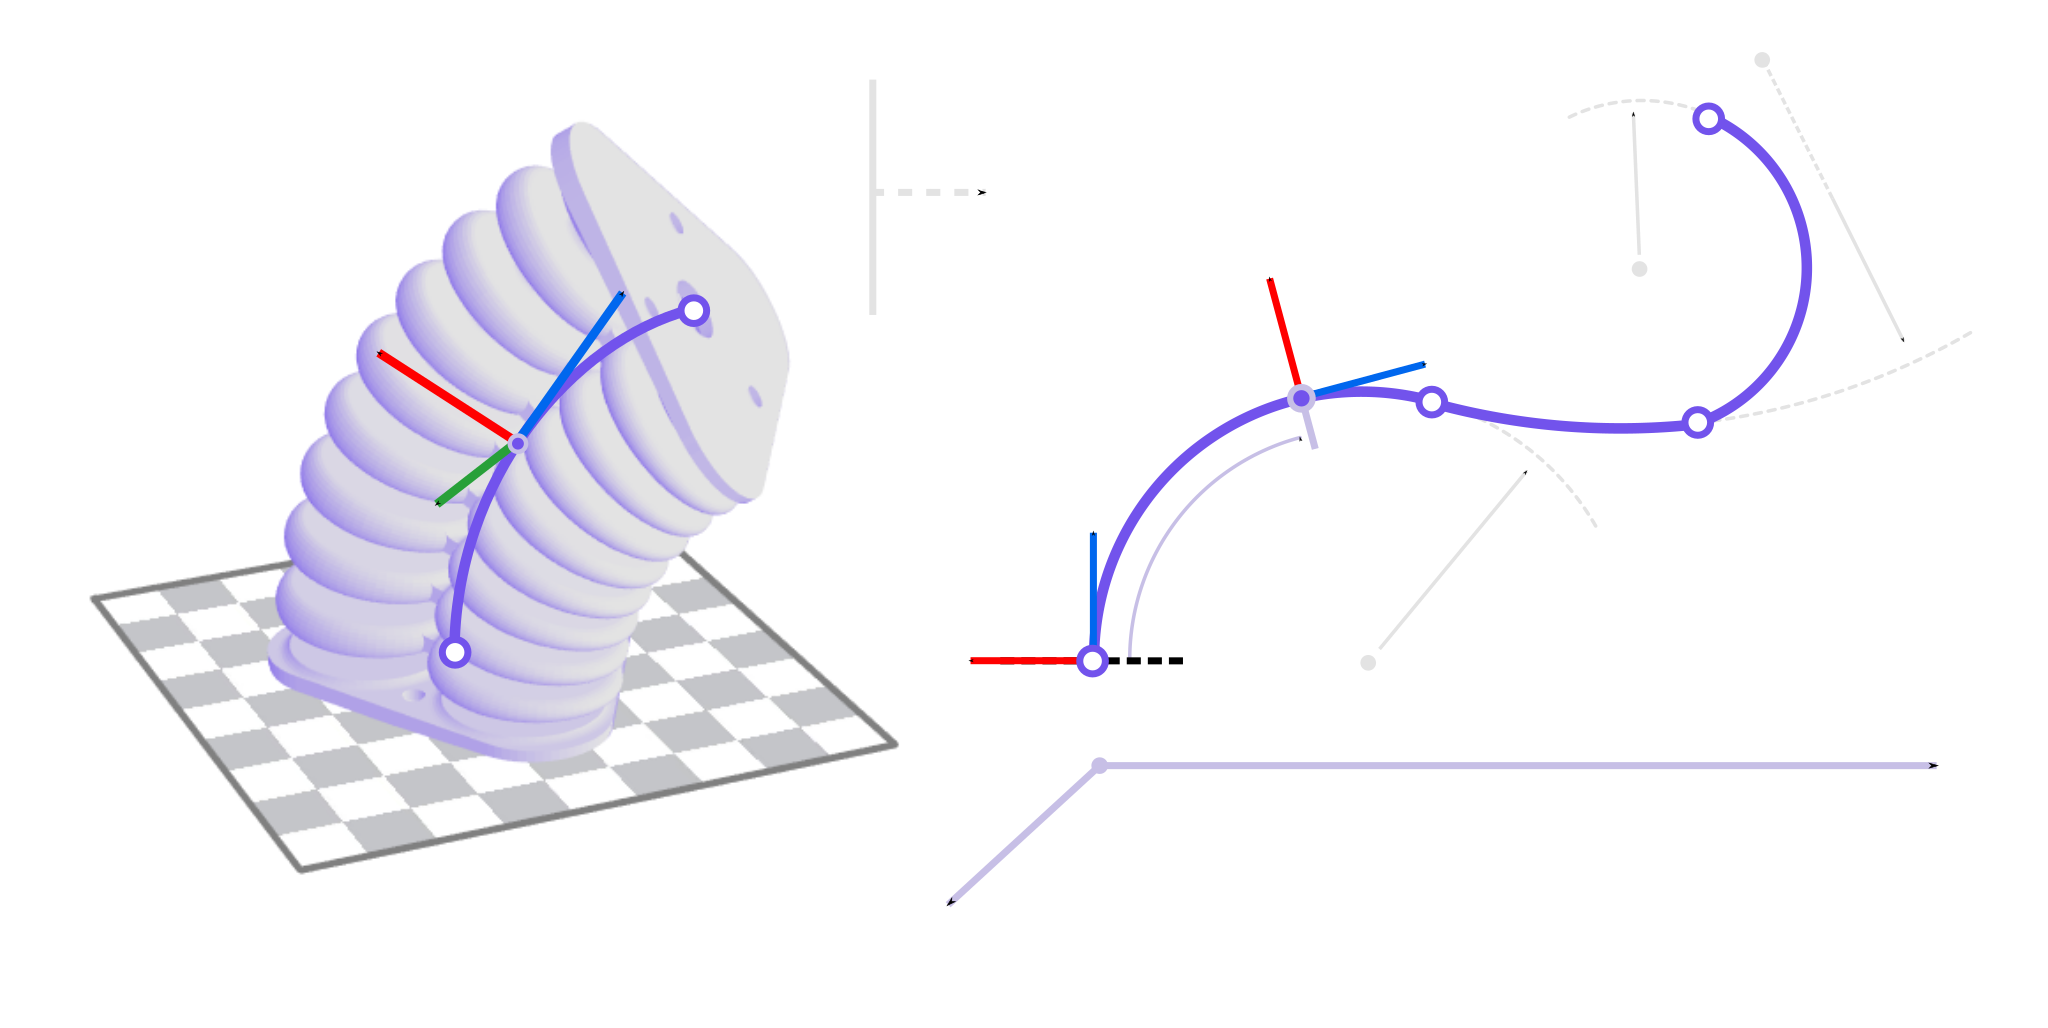
\includegraphics[width = 0.99\textwidth]{fig_C2_schematic.pdf}
  \fi
  \caption{Schematic representation of the Piece-wise Constant Curvature model (PCC) for general soft robotic system, given by a parameterized curve $^0 \gammaB: \Xs \times \Ts \to \R^3$ and orientation matrix $^0 \PhiB: \Xs \times \Ts \to \SO{3}$. The frame $\{\sigma\}$ is rigidly attached to $^0 \gammaB$ such that variation of $\sigma$ give insight into the differential geometry of the curve.}
  \label{fig:C2:configuration}
\end{figure}
%
\begin{dfn}[Piece-wise Constant Curvature]
Despite the inherent flexibility in soft robotics, it is sometimes sufficient to express the kinematics according to the \emph{Piecewise Constant Curvature} (PCC) condition. Mathematically, it implies that the curvature of the continuous body satisfies $\kappa(\sigma_1,\q) = \kappa(\sigma_2,\q)$ for a neighboring region of points $\sigma_1,\sigma_2 \subseteq \Xs$. As a result, this condition allows us to describe the full forward kinematics with a significantly reduced set of generalized coordinates, mitigating kinematic complexity in the model. Numerous works employ PCC models \cite{Falkenhahn2015,Katzschmann2019,Tatlicioglu2007,Marchese2016,Godage2016,DellaSantina2020a}, and depending on the elasticity, the PCC condition has been proven to be consistent for various soft robotic systems.
\end{dfn}
%
{Following this Constant Curvature (CC) description, let us assign a coordinate frame that twists minimally along the backbone -- formally called the \emph{Bishop frame} (see, \cite{Bishop1975}) -- parametrized by the following generalized coordinate vector:}
%
\begin{equation}
\vec{q} := \begin{pmatrix}
\,\varepsilon & \kappa_x & \kappa_y\,
\end{pmatrix}^\top \in \mathcal{Q},
\label{eq:C2:coordinate}
\end{equation}
%
\noindent where $\varepsilon_{-} \le \varepsilon \le \varepsilon_{+}$ is the elongation strain, and $\kappa_x,\,\kappa_y\in\mathbb{R}$ are the curvatures or angular strains in $x$-$z$ and $y$-$z$ plane, respectively; and
$\mathcal{Q} \subset \R^3$ is an admissible space on which $\q$ evolves. Also, we denote the total curvature by $\kappa = \inner{\kappa_x}{\kappa_y}$ together with the curvature angle $\phi = \atantwo(\kappa_y,\kappa_x)$. It is worth mentioning that the joint description above is somewhat related to Renda. et al. (2018, \cite{Renda2018}) who proposed a \emph{Piece-wise Constant Strain} (PCS) parametrization with the exception of including the twist along the tangent.

By exploring the differential geometry of the smooth backbone curve similar to Mochiyama et al. (2003, \cite{Mochiyama2003}), we can write the position vector $\gammaB(\sigma,\q)$ and the orientation matrix $\PhiB(\sigma,\q)$ for each material point $\sigma$ along the smooth backbone as a differential equality of the form:
%
\begin{align}
\renewcommand*{\arraystretch}{2}{}
\frac{\partial \,\!\mat{\Phi}}{\partial \sigma}(\sigma,\q) & = \, \mat{\Phi}(\sigma,\vec{q}) \,\mat{\Gamma}^{\times} (\sigma,\q) \label{eq:C2:change_phi} \\[0.45em]
%
\frac{\partial \, \gammaB}{\partial \sigma}(\sigma,\q) & = \, \mat{\Phi}(\sigma,\vec{q}) \, \vec{U}(\sigma,\q), \label{eq:C2:change_p}
\end{align}
%
where $\vec{\Gamma}^\times \in \SO{3}$ is a skew-symmetric matrix composed of the entries of the vector $\vec{\Gamma} \in \R^3$, and $\vec{U}\in \R^3$ a vector representing the tangent along the extensible backbone. For readers familiar with Lie Groups, the operator $(\,\cdot\,)^\times$ denotes the isomorphism between the Lie algebra $\sog{3}$ and $\R^3$. The vectors $\vec{\Gamma}$ and $\vec{U}$ are vectors that define the differential geometry of the backbone
\cite{Mochiyama2003} which are unique entries that live in the tangent space of the rigid-body transformation group, \ie, $T_{\SE{3}}$. Given the Bishop parametrization as described by \eqref{eq:C2:coordinate} and assuming the Constant-Strain (CC) condition, these geometric entities yield
%
\begin{align}
\vec{\Gamma}(\sigma,t) & \cong \vec{\Gamma}(\sigma,\q(t)) \quad \xRightarrow[]{\textrm{CC condition}}\quad \vec{\Gamma}(\q) = \begin{pmatrix} \;-\kappa_y\;\; \\ \;\kappa_x\;\; \\ \;0\;\;  \end{pmatrix}, \\[0.35em]
%
\vec{U}(\sigma,t) & \cong \vec{U}(\sigma,\q(t)) \!\quad \xRightarrow[]{\textrm{CC condition}} \quad \vec{U}(\q) =  \begin{pmatrix} \;0\;\;  \\  \;0\;\; \\ \varepsilon + 1\ \end{pmatrix},
\end{align}
%
%with $\vec{U}^\circ$ the unit-tangent pointing, and $\vec{\Gamma}^\circ$ the intrinsic curvature/torsion of the curve. For simplicity, lets assume $\vec{U}^\circ = (0,0,1)^\top$ and $\vec{\Gamma}^\circ = \vec{0}_3$.
Now, given an initial configuration of backbone's base, \ie,$\mat{\Phi}(0,\vec{q}) = \vec{\Phi}_0$ and $ \gammaB(0,\q) = \vec{0}_3$, we can now solve for the position and orientation for each material coordinate $\sigma$ along the backbone:
%
\begin{align}
\mat{\Phi}(\sigma,\vec{q}) & = \vec{\Phi}_0\exp_{\SO{3}}(\sigma \vec{\Gamma}^\times(\vec{q})), \label{eq:C2:phi_exact} \\[0.35em]
\gammaB(\sigma,\vec{q}) & = \int_0^\sigma\,^0\mat{\Phi}(\eta,\vec{q})\, \vec{U}(\vec{q}) \; d\eta,
\label{eq:C2:pos_exact}
\end{align}
%
where $\exp_{\SO{3}}: \sog{3} \to \SO{3}$ is the exponential map. Luckily, there exist a compact expression for the exponential mapping related to the orthogonal group of rotation matrices $\SO{3}$ called the \emph{Rodriguez formulas}. Given the rotation angle $\theta(\sigma,\q) := \int_0^\sigma \kappa(s,\q) \; ds = \kappa(\q) \sigma$, we can compactly rewrite the rotation matrix \eqref{eq:C2:phi_exact} in terms of $\cos(\theta)$ and $\sin(\theta)$ using these formulas as follows \cite{Lynch2017}:
%
\begin{equation}
\PhiB(\theta) = \PhiB_0 \left( \mat{I}_3 + \left[ \frac{\sin(\theta)}{\theta} \right]  \GammaB^{\times} + \left[ \frac{1-\cos(\theta)}{\theta^2} \right]  \GammaB^{\times} \GammaB^{\times} \right).
\label{eq:C2:phi_rodr}
\end{equation}
%
We wish to inform the reader that the closed-form solutions \eqref{eq:C2:phi_exact} and \eqref{eq:C2:pos_exact} represent the forward configuration kinematics of the backbone curve. To express the forward velocity kinematic, let
$\etaB(\sigma,\q,\dq) = \left( \vec{\omega}^\top, \vec{v}^\top \right)^\top \in \R^6 \cong \seg{3}$
 be the aggregate of the angular velocity and linear velocity components relative to an inertial frame at $\sigma$, where the space $\seg{3}$ denotes the Lie algebra of $\SE{3}$. The velocity twist is computed by the following integration procedure:
%
\begin{align}
 \etaB(\sigma,\q,\dq) = \Ad_{\mat{g}(\sigma,\cdot)}\inv \int_0^\sigma \Ad_{\mat{g}(s,\cdot)}\, \JB^\star\! \dq\;ds
 \,=:\, \JB(\q,\sigma) \dq, \label{eq:C2:vel_cont}
\end{align}
%
where $\Ad_g: \SE{3} \to \mathbb{R}^{6\times 6}$ denotes the adjoint transformation matrix regarding the rigid body transformation $\gB \in \SE{3}$ that maps local velocities (i.e., twist) to a frame located at $\sigma$, and $\JB^\star:\Q \to T_{\q}\Q$ the joint-axis matrix that relates the DOFs to the geometric deformations. Let it be clear that the joint-axis matrix is naturally constant for a soft segment modeled with the Constant-Strain (CS) assumption. We will later relax this assumption in Chapter 4. Nevertheless here, the joint-axis matrix for an extensible and bendable CS segment parametrized by the Bishop parameters is given by
%
\begin{align}
\renewcommand*{\arraystretch}{1}{}
\JB^\star := \begin{pmatrix}\dfrac{\p \GammaB}{\p \q}^\top & \dfrac{\p \UB}{\p \q}^\top \end{pmatrix}^\top  = \begin{pmatrix}
\,0 & 0 & 0 & 0 & 0 & 1 \, \\
\,0 & 1 & 0 & 0 & 0 & 0 \,  \\
\,-1 & 0 & 0 & 0 & 0 & 0 \,  \\
\end{pmatrix}^\top. \label{eq:C2:joint-axis-matrix}
\end{align}
%
Although we based the forward kinematics on the work of Mochiyama et al.\cite{Mochiyama2003}, the derived expression for the velocity twist in \eqref{eq:C2:vel_cont} is analogous to the work of Renda et al. (2018, 2020; \cite{Renda2018,Renda2020}), and Boyer et al. (2010, 2021; \cite{Boyer2010,Boyer2021}). Please also note that
\eqref{eq:C2:vel_cont} gives rise to the geometric manipulator Jacobian $\JB(\sigma,\q)$ that defines the mapping from joint velocities to the velocity twist for a point $\sigma$ on the elastic body.

In continuation, let us also introduce the acceleration twist \cite{Boyer2021,Mochiyama2003,Renda2018} -- obtained through time differentiation of \eqref{eq:C2:vel_cont}:
%
\begin{align}
\dot{\etaB}(\sigma,\q,\dq,\ddq) & = \JB \ddot{\q} + \Ad_{\gB(\cdot,\sigma)} \inv \int_0^\sigma \Ad_{\gB(s,\cdot)}
\ad_{\etaB(s,\cdot,\cdot)} \, \JB^\star\! \dq \;ds \notag \\
& :=  \JB(\sigma,\q)\ddot{\q} + \dmat{J}(\sigma,\q,\dot{\q}) \dot{\q},
\label{eq:C2:acceleration}
\end{align}
%
where $\ad_{\etaB}: \R^{6} \to \R^{6\times 6}$ denotes the adjoint transformation regarding the velocity twist $\vec{\etaB}^\wedge \in \seg{3}$. The reader is referred to Appendix \ref{app:C2:adjoint} for more detailed expressions on the adjoint transformations.
%
\begin{rmk}[Numerical instability near zero-curvature] In many of the PCC modeling literate there are mentions of a singularity point when the soft robot $\kappa \to 0$, stating that the linear velocities $\vec{v} := \floor{\etaB}_3$ are not well-defined and thus may be unbounded. However, this is perhaps a common misconception in literate is mainly caused by numerical instability. To illustrate, consider the inextensible planar case: $\varepsilon = \kappa_y = 0$ and $\kappa = \kappa_x$. Hence, by solving the forward kinematics for the position vector $\gammaB(\sigma,\kappa)$, and taking the approaching zero from the positive domain $\kappa^{+} \to 0$, we see that
%
\begin{align}
\lim_{\kappa \to \,0^{+}}\gammaB(\sigma,\kappa) & = \begin{pmatrix} \dfrac{1-\cos(\sigma \kappa)}{\kappa}\,, & 0\,, & \dfrac{\sin(\sigma \kappa)}{\kappa} \end{pmatrix}^\top = \begin{pmatrix} 0 & 0 & \sigma \end{pmatrix}^\top,
\end{align}
%
which is clearly well-defined. Since the position vector $\gammaB$ is continuously differentiable when approaching the origin from both sides $\kappa \to 0^+$ and $\kappa \to 0^{-}$, it follows that $\dot{\gammaB}$ must be bounded for all $\kappa \in \Q$. We can simply check this by investigating the behavior of the linear-velocity portion of the geometric Jacobian near zero-curvature, which yields
%
\begin{align}
\lim_{\kappa \to \,0^+} \floor{\JB}_3(\sigma,\kappa) & = \begin{pmatrix} \tfrac{\sigma \kappa \sin(\sigma \kappa) + 1 - \cos(\sigma \kappa)}{\kappa^2}\,, & 0\,, & \tfrac{\sigma \kappa \cos(\sigma \kappa) - \sin(\sigma \kappa) }{\kappa^2} \end{pmatrix}^\top \notag \\[0.35em] & = \begin{pmatrix} \sigma^2 & 0 & 0 \end{pmatrix}^\top.
\end{align}
%
Again, the expression is well-defined. Consequently, the magnitude of the linear velocity of the end-effector reads simply $\lVert \dot{\gammaB}(L,\dot{\kappa}) \rVert = L^2\dot{\kappa} = L \omega_1$ with $\omega_1$ the angular velocity at the tip. This naturally poses an ambiguity on the origin of this kinematic singularity. The problem is, however, of numerical origin when considering the zero-division. To make matters worse, deriving analytical expressions for accelerations will contain similar expressions that are hard to stabilize numerically. To resolve this issue, we opt for a numerical approximation of the forward kinematics -- namely, we employ an explicit forward integration scheme (\ie, trapezoidal integration) to solve \eqref{eq:C2:change_phi} and \eqref{eq:C2:change_p}.
\end{rmk}

\newpage
\begin{example}[Kinematic behavior of PCC segment]
As an illustrative example, we provide simulation of the forward kinematics for a single PCC segment given predefined trajectory on the geometric join variables $\q(t) \equiv \q_d(t)$, $\dot{\q}(t) \equiv \dot{\q}_d(t)$ and $\ddot{\q}(t) \equiv \ddot{\q}_r(t)$. Let us consider the following reference trajectory for the 3-DOF soft manipulator:
%
\begin{align*}
\q_d(t) &  =  \erf(t) \cdot \begin{pmatrix} \varepsilon_0 \sin(\omega t) & \kappa_0 \cos(\omega t) & \kappa_0 \sin(\tfrac{3}{2}\omega t - \tfrac{\pi}{4}) \end{pmatrix}^\top,
\end{align*}
%
where $\textrm{erf}(t) := \frac{2}{\pi}\int_0^\tau \exp(-\tau^2) \; d\tau$ is referred to as the error function. Note that these are smooth functions such that reference velocity $\dq_d$ and reference acceleration $\ddq_d$ exist and are bounded. The reference signals for the geometric strain of the soft robot are shown in Figure \ref{fig:C2:EX1:strain_ref}. Let it be clear that the reference $\q_d$ has been carefully selected to ensure it passes the line $\kappa_x = \kappa_y = 0$ on the configuration space
$\mathcal{Q}$, \ie, the numerical instability point for near-zero curvature..

Then, by inject the reference into the kinematic relations described by the expressions \eqref{eq:C2:change_phi}, \eqref{eq:C2:change_p}, \eqref{eq:C2:vel_cont}, and \eqref{eq:C2:acceleration}, we obtain a (close) approximation of forward kinematics as shown in Figure
\ref{fig:C2:EX1:strain_ref_FK}. Furthermore, we provided a 3D-rendering of the soft robot subjected to the reference $\q_d$ in Figure \ref{fig:C2:EX1:strain_ref_3D}. Now, two key observations can be made. First, although a simple harmonic trajectory is used, the resulting trajectory of the end-effector as shown in Figure \ref{fig:C2:EX1:strain_ref_FK} is rather complex. This perhaps stresses the importance of inverse kinematic solver that can be used for task-space control. Second, although we pass the point of numerical instability for
$\kappa \to 0$, we see that the velocity solutions are smooth and bounded at these instances. This result shows our approach does not suffer from the near-zero curvature instabilities that are notoriously mentioned in \cite{Falkenhahn2015,DellaSantina2020}, yet at the cost of providing an analytical expression.

\begin{figure}[!b]
  %\vspace{-0mm}
  %\centering
  \ifx\printFigures1\undefined
  \else
  % This file was created by matlab2tikz.
%
\definecolor{mycolor1}{rgb}{0.00000,0.34510,0.65882}%
\definecolor{mycolor2}{rgb}{0.79216,0.11765,0.17255}%
\definecolor{mycolor3}{rgb}{0.20392,0.65490,0.24706}%
%
\begin{tikzpicture}

\begin{axis}[%
width=0.248\textwidth,
height=0.19\textwidth,
at={(0\textwidth,0\textwidth)},
scale only axis,
xmin=0,
xmax=5,
xlabel style={font=\color{white!15!black}},
xlabel={time (s)},
ymin=-2,
ymax=2,
ylabel style={font=\color{white!15!black}},
ylabel={$q_d$},
axis background/.style={fill=white},
xmajorgrids,
ymajorgrids,
ylabel style={yshift=-7.5pt}
]
\addplot [color=mycolor1, line width=1.5pt, forget plot]
  table[row sep=crcr]{%
0	0\\
0.035035035035035	0.00434065382436177\\
0.075075075075075	0.0197581919620422\\
0.115115115115115	0.0457558239801097\\
0.16016016016016	0.0864034559537759\\
0.215215215215215	0.149650792611576\\
0.29029029029029	0.251909193908196\\
0.435435435435435	0.452501851145034\\
0.49049049049049	0.511874966215594\\
0.535535535535535	0.547735702552471\\
0.575575575575575	0.567954316778994\\
0.61061061061061	0.575566933229249\\
0.645645645645645	0.573088771427073\\
0.68068068068068	0.560095653946306\\
0.715715715715715	0.536392535810649\\
0.755755755755755	0.496246230155413\\
0.795795795795796	0.442585433729294\\
0.840840840840841	0.367062318903137\\
0.895895895895896	0.255345156916537\\
0.960960960960961	0.101033017828754\\
1.05605605605606	-0.15149073785141\\
1.20620620620621	-0.550319348528045\\
1.27627627627628	-0.708764889034357\\
1.33133133133133	-0.811325353645943\\
1.37637637637638	-0.877772299605288\\
1.41641641641642	-0.922105295564261\\
1.45145145145145	-0.948751619733451\\
1.48648648648649	-0.963596043213059\\
1.51651651651652	-0.966718567647844\\
1.54654654654655	-0.960902245684151\\
1.57657657657658	-0.946171019746461\\
1.61161161161161	-0.91787491799227\\
1.65165165165165	-0.871308378489516\\
1.6966966966967	-0.801691383211872\\
1.74674674674675	-0.704652917692613\\
1.8018018018018	-0.576880303587744\\
1.87187187187187	-0.388564855615353\\
1.96696696696697	-0.103030019623617\\
2.15715715715716	0.472826180715402\\
2.22722722722723	0.653682856913231\\
2.28728728728729	0.783947303234589\\
2.33733733733734	0.871419229432251\\
2.38238238238238	0.931802645757189\\
2.42242242242242	0.969852863853533\\
2.45745745745746	0.990576346388929\\
2.48748748748749	0.99879275130267\\
2.51751751751752	0.998116211770342\\
2.54754754754755	0.988552949224476\\
2.58258258258258	0.966282396359661\\
2.61761761761762	0.932306066362887\\
2.65765765765766	0.87967759968175\\
2.7027027027027	0.803890788095862\\
2.75275275275275	0.700895927035849\\
2.81281281281281	0.554714287228555\\
2.88788788788789	0.344958268771602\\
3.003003003003	-0.00943386773232557\\
3.14314314314314	-0.43468926190012\\
3.21821821821822	-0.633097599682777\\
3.27827827827828	-0.767051472600784\\
3.32832832832833	-0.858054673447568\\
3.37337337337337	-0.921910196927753\\
3.41341341341341	-0.963228857786627\\
3.44844844844845	-0.986913031185399\\
3.48348348348348	-0.998653274574725\\
3.51351351351351	-0.999098293329462\\
3.54354354354354	-0.990657463060607\\
3.57857857857858	-0.96968362697153\\
3.61361361361361	-0.936974398085302\\
3.65365365365365	-0.885736697748763\\
3.6986986986987	-0.811413049476992\\
3.74874874874875	-0.709880810775015\\
3.80880880880881	-0.565174526154613\\
3.88388388388388	-0.356752674288018\\
3.99399399399399	-0.0188673044788441\\
4.14414414414414	0.437523008440333\\
4.21921921921922	0.635532084307429\\
4.27927927927928	0.769068005472834\\
4.32932932932933	0.859667579389312\\
4.37437437437437	0.923125598625732\\
4.41441441441441	0.964070346402118\\
4.44944944944945	0.987416293148271\\
4.48448448448448	0.998812274000765\\
4.51451451451451	0.998960559587034\\
4.54454454454454	0.990224253362287\\
4.57957957957958	0.968910783145196\\
4.61461461461461	0.935871305490616\\
4.65465465465465	0.884272782967919\\
4.6996996996997	0.809571163316425\\
4.74974974974975	0.707662478873392\\
4.80980980980981	0.562577458212637\\
4.88488488488488	0.353813119124604\\
5	8.88178419700125e-16\\
};
\addplot [color=mycolor2, line width=1.5pt, forget plot]
  table[row sep=crcr]{%
0	0\\
0.105105105105105	0.111779765028618\\
0.16016016016016	0.156980153648786\\
0.205205205205205	0.182511422079791\\
0.245245245245245	0.194668024428809\\
0.28028028028028	0.196227360736436\\
0.315315315315315	0.188769317384463\\
0.35035035035035	0.172022106528288\\
0.39039039039039	0.141487076700804\\
0.43043043043043	0.0991512285511922\\
0.475475475475475	0.0383838014112809\\
0.53053053053053	-0.0523767761630261\\
0.6006006006006	-0.18783198174113\\
0.840840840840841	-0.67188191620076\\
0.895895895895896	-0.752708585608064\\
0.940940940940941	-0.802692146771466\\
0.980980980980981	-0.833165316743078\\
1.01601601601602	-0.848168474733675\\
1.04604604604605	-0.851956160757179\\
1.07607607607608	-0.847156376186706\\
1.10610610610611	-0.833681829324347\\
1.14114114114114	-0.807033343602345\\
1.17617617617618	-0.768832354621136\\
1.21621621621622	-0.711564770634355\\
1.26126126126126	-0.63088812208567\\
1.31631631631632	-0.511373504538406\\
1.38138138138138	-0.345607907267669\\
1.46646646646647	-0.101148746562225\\
1.68668668668669	0.544000207265759\\
1.75175175175175	0.701576721741857\\
1.80680680680681	0.812683401978535\\
1.85685685685686	0.892797948975148\\
1.8968968968969	0.941073870130205\\
1.93193193193193	0.971074104183863\\
1.96696696696697	0.989241847338064\\
1.996996996997	0.995215537037103\\
2.02702702702703	0.992264006504053\\
2.05705705705706	0.980411255152744\\
2.09209209209209	0.95547795269928\\
2.12712712712713	0.918880529317171\\
2.16716716716717	0.863353759912902\\
2.21221221221221	0.7844957377737\\
2.26726726726727	0.666829747058395\\
2.33233233233233	0.502232140204002\\
2.41241241241241	0.271529840930044\\
2.7027027027027	-0.594554525970798\\
2.76776776776777	-0.745387426665372\\
2.82282282282282	-0.848990849411984\\
2.86786786786787	-0.915028120952007\\
2.90790790790791	-0.958401759441889\\
2.94294294294294	-0.983946634072939\\
2.97797797797798	-0.997582418387913\\
3.00800800800801	-0.999662561645784\\
3.03803803803804	-0.992851132434541\\
3.06806806806807	-0.977208771789291\\
3.1031031031031	-0.947988039568602\\
3.14314314314314	-0.900570748735437\\
3.18818818818819	-0.830261109785634\\
3.23823823823824	-0.732742817227718\\
3.29329329329329	-0.604697368948116\\
3.36336336336336	-0.41619419138787\\
3.45845845845846	-0.1301363223696\\
3.65365365365365	0.464187490802019\\
3.72372372372372	0.646393867785127\\
3.78378378378378	0.778035686293484\\
3.83383383383383	0.866810466126059\\
3.87887887887888	0.928474109611159\\
3.91891891891892	0.967732918025878\\
3.95395395395395	0.989555253702245\\
3.98398398398398	0.998734409694203\\
4.01401401401401	0.999030984234652\\
4.04404404404404	0.990442339782819\\
4.07907907907908	0.969298597922351\\
4.11411411411411	0.9364241544223\\
4.15415415415415	0.88500593597636\\
4.1991991991992	0.810493174479892\\
4.24924924924925	0.708772560434584\\
4.30930930930931	0.563876708920316\\
4.38438438438438	0.35528334276137\\
4.49449449449449	0.0172951932970005\\
4.63963963963964	-0.424754659261413\\
4.71471471471471	-0.624542944420901\\
4.77477477477477	-0.759946247977657\\
4.82482482482482	-0.852352489109542\\
4.86986986986987	-0.917592188634139\\
4.90990990990991	-0.96021468537402\\
4.94494494494494	-0.985079574464464\\
4.97997997997998	-0.99802277725853\\
5	-0.999999999998463\\
};
\addplot [color=mycolor3, line width=1.5pt, forget plot]
  table[row sep=crcr]{%
0	-0\\
0.04004004004004	-0.0253745100040801\\
0.07007007007007	-0.0347038050172159\\
0.1001001001001	-0.0347370008429007\\
0.13013013013013	-0.0250154145793022\\
0.16016016016016	-0.0054932552761473\\
0.195195195195195	0.0291506297466535\\
0.235235235235235	0.0827538361897568\\
0.285285285285285	0.16619460726963\\
0.46046046046046	0.476679866800188\\
0.5005005005005	0.520938149913881\\
0.53053053053053	0.541265433708041\\
0.555555555555555	0.548589477479468\\
0.58058058058058	0.546477201874926\\
0.605605605605605	0.534475742154076\\
0.63063063063063	0.512334606754345\\
0.66066066066066	0.472339342305941\\
0.695695695695695	0.407638563999009\\
0.735735735735735	0.311549516304309\\
0.785785785785786	0.162988678062016\\
0.850850850850851	-0.0635843329845418\\
1.001001001001	-0.598978538317431\\
1.05105105105105	-0.737906954073797\\
1.09109109109109	-0.822134211231833\\
1.12112112112112	-0.866793223366643\\
1.14614614614615	-0.890778796998402\\
1.17117117117117	-0.902132835176695\\
1.19119119119119	-0.901877449005232\\
1.21121121121121	-0.893224311557399\\
1.23623623623624	-0.870611388147704\\
1.26126126126126	-0.835084370833918\\
1.29129129129129	-0.775989311963286\\
1.32632632632633	-0.685754032567514\\
1.37137137137137	-0.539824281580024\\
1.42642642642643	-0.324964646431106\\
1.51151151151151	0.0524552962322513\\
1.61661661661662	0.51068147425186\\
1.67167167167167	0.710508039285358\\
1.71671671671672	0.839809432175977\\
1.75175175175175	0.914737029146651\\
1.78178178178178	0.959240382698092\\
1.80680680680681	0.981667705873682\\
1.82682682682683	0.989754892345688\\
1.84684684684685	0.988985560607153\\
1.86686686686687	0.979356598439477\\
1.89189189189189	0.954987957816951\\
1.91691691691692	0.917231880765766\\
1.94694694694695	0.854996252662267\\
1.98198198198198	0.760654843428203\\
2.02702702702703	0.609027332372115\\
2.08208208208208	0.386868838337833\\
2.16716716716717	-0.00235341420373558\\
2.27227227227227	-0.476740013733818\\
2.32732732732733	-0.686128439736638\\
2.37237237237237	-0.823872463922093\\
2.40740740740741	-0.905707232186816\\
2.43743743743744	-0.956312435519591\\
2.46246246246246	-0.983906356917698\\
2.48748748748749	-0.997827816311879\\
2.50750750750751	-0.99898359601381\\
2.52752752752753	-0.991250100548469\\
2.55255255255255	-0.969194596213682\\
2.57757757757758	-0.933668618821868\\
2.60760760760761	-0.873964134919092\\
2.64264264264264	-0.782315745941585\\
2.68768768768769	-0.633618002235095\\
2.74274274274274	-0.414005821608413\\
2.82282282282282	-0.0495061227704499\\
2.94294294294294	0.493844251052776\\
2.997997997998	0.700388748460756\\
3.04304304304304	0.835041499681637\\
3.07807807807808	0.914107856575382\\
3.10810810810811	0.962155969131873\\
3.13313313313313	0.98753105117545\\
3.15815815815816	0.99918833543435\\
3.17817817817818	0.998522048373447\\
3.1981981981982	0.988974942633285\\
3.22322322322322	0.964689233243766\\
3.24824824824825	0.927003009137534\\
3.27827827827828	0.864840650298925\\
3.31331331331331	0.770571225684974\\
3.35835835835836	0.619000071754701\\
3.41341341341341	0.396800981518273\\
3.4984984984985	0.00707559477390074\\
3.60860860860861	-0.489752472097759\\
3.66366366366366	-0.697029667042679\\
3.70870870870871	-0.832450937165657\\
3.74374374374374	-0.912197337060987\\
3.77377377377377	-0.960870579525157\\
3.7987987987988	-0.986786943557313\\
3.82382382382382	-0.998996023815813\\
3.84384384384384	-0.998773604988724\\
3.86386386386386	-0.989668255700024\\
3.88888888888889	-0.965925789545627\\
3.91391391391391	-0.928765818557316\\
3.94394394394394	-0.86720224931259\\
3.97897897897898	-0.77357123059458\\
4.02402402402402	-0.622699193733973\\
4.07907907907908	-0.401126949383538\\
4.16416416416416	-0.0117924918369763\\
4.27427427427427	0.485634538435109\\
4.32932932932933	0.693639713954403\\
4.37437437437437	0.82982807333996\\
4.40940940940941	0.910254465460059\\
4.43943943943944	0.959553358610013\\
4.46446446446446	0.986011765731368\\
4.48948948948949	0.998773659190625\\
4.50950950950951	0.998996087409785\\
4.52952952952953	0.990333607846368\\
4.55455455455455	0.967135952108439\\
4.57957957957958	0.930503983273733\\
4.60960960960961	0.869541525097858\\
4.64464464464464	0.776551901449321\\
4.68968968968969	0.626383213058514\\
4.74474474474474	0.405443448982906\\
4.82982982982983	0.0165091212806967\\
4.93993993993994	-0.481505636914043\\
4.99499499499499	-0.690234174264289\\
5	-0.707106781185458\\
};
\end{axis}

\begin{axis}[%
width=0.248\textwidth,
height=0.19\textwidth,
at={(0.326\textwidth,0\textwidth)},
scale only axis,
xmin=0,
xmax=5,
xlabel style={font=\color{white!15!black}},
xlabel={time (s)},
ymin=-0.04,
ymax=0.04,
ylabel style={font=\color{white!15!black}},
ylabel={$\dot{q}_d$},
axis background/.style={fill=white},
xmajorgrids,
ymajorgrids,
ylabel style={yshift=-7.5pt}
]
\addplot [color=mycolor1, line width=1.5pt, forget plot]
  table[row sep=crcr]{%
0	8.87958036743797e-05\\
0.02002002002002	0.000709205286566927\\
0.13013013013013	0.00431354598848444\\
0.2002002002002	0.00602568516306956\\
0.26026026026026	0.00693784257997976\\
0.32032032032032	0.00724490259747501\\
0.38038038038038	0.00690746540709775\\
0.44044044044044	0.00593471651671429\\
0.505505505505505	0.00422996742472659\\
0.575575575575575	0.00177973755126715\\
0.675675675675675	-0.00240049325539715\\
0.825825825825826	-0.00868090425285217\\
0.900900900900901	-0.0111658143824966\\
0.965965965965966	-0.0127084883031694\\
1.02602602602603	-0.0135312743668141\\
1.08608608608609	-0.0137280496105907\\
1.14614614614615	-0.0132868669616926\\
1.20620620620621	-0.0122291022584786\\
1.27127127127127	-0.0104477195110757\\
1.34134134134134	-0.0079022607533874\\
1.42642642642643	-0.00416316463676836\\
1.58658658658659	0.00368059325814496\\
1.69169169169169	0.00849151878580301\\
1.77177177177177	0.0115460906314997\\
1.84184184184184	0.0136041791124057\\
1.90690690690691	0.0149070651732561\\
1.96696696696697	0.0155416553906065\\
2.02702702702703	0.0156092580414757\\
2.08708708708709	0.0151099515853312\\
2.15215215215215	0.0139534009546507\\
2.21721721721722	0.01220713173322\\
2.29229229229229	0.00955913862891311\\
2.37737737737738	0.0059220893298475\\
2.5025025025025	-0.000112795085106754\\
2.65265265265265	-0.00724892771459817\\
2.73773773773774	-0.0106779731168718\\
2.80780780780781	-0.012940911941616\\
2.87287287287287	-0.0144843869759752\\
2.93793793793794	-0.0154244334183069\\
2.997997997998	-0.0157223717405444\\
3.05805805805806	-0.0154620801493941\\
3.12312312312312	-0.0145613972166379\\
3.18818818818819	-0.0130543490417994\\
3.25825825825826	-0.0108257718717653\\
3.33833833833834	-0.00764650755058938\\
3.43843843843844	-0.00302197280326677\\
3.67867867867868	0.00836963830915671\\
3.75875875875876	0.0114195404408468\\
3.82882882882883	0.0135039386224447\\
3.89389389389389	0.0148575485231452\\
3.95895895895896	0.0155925293693473\\
4.01901901901902	0.01569498110561\\
4.07907907907908	0.0152403197954696\\
4.14414414414414	0.0141382701809354\\
4.20920920920921	0.0124475408105065\\
4.27927927927928	0.0100496470917113\\
4.36436436436436	0.00649885919009208\\
4.47947947947948	0.00101291704575601\\
4.65465465465465	-0.00734219873027886\\
4.73973973973974	-0.0107537859157611\\
4.80980980980981	-0.0129989373491224\\
4.87487487487487	-0.0145238276366495\\
4.93993993993994	-0.0154439846312249\\
5	-0.0157230390570149\\
};
\addplot [color=mycolor2, line width=1.5pt, forget plot]
  table[row sep=crcr]{%
0	0.00564679810898916\\
0.06006006006006	0.00532698853810398\\
0.12012012012012	0.00439279220918198\\
0.185185185185185	0.00277385963725596\\
0.265265265265265	0.000135489686829082\\
0.51051051051051	-0.00846723701053786\\
0.575575575575575	-0.00988340148525158\\
0.635635635635635	-0.0105965516072484\\
0.695695695695695	-0.0106745781731705\\
0.755755755755755	-0.0100982489775987\\
0.815815815815816	-0.00889075730022348\\
0.880880880880881	-0.00694328214617457\\
0.950950950950951	-0.00424090998455195\\
1.04604604604605	8.04961082803146e-05\\
1.23623623623624	0.0088695371597316\\
1.31131131131131	0.0116449451465765\\
1.37637637637638	0.0134795293660801\\
1.43643643643644	0.0146177117690955\\
1.4964964964965	0.0151759125248292\\
1.55655655655656	0.0151350477011531\\
1.61661661661662	0.014501321548952\\
1.68168168168168	0.0131809237407268\\
1.74674674674675	0.0112662147885771\\
1.82182182182182	0.00843852080878538\\
1.91191191191191	0.00440679951085077\\
2.21721721721722	-0.00986682322024279\\
2.29229229229229	-0.0124599594878632\\
2.36236236236236	-0.0142550761271227\\
2.42742742742743	-0.0153034838841499\\
2.48748748748749	-0.015703599140477\\
2.54754754754755	-0.0155443311943841\\
2.61261261261261	-0.0147481695643945\\
2.67767767767768	-0.0133367782902223\\
2.74774774774775	-0.0111971986946333\\
2.82282282282282	-0.00830788352575418\\
2.91791791791792	-0.00401063830401949\\
3.2032032032032	0.00936909186312107\\
3.27827827827828	0.0120603023051942\\
3.34834834834835	0.0139720380102135\\
3.41341341341341	0.0151448717266796\\
3.47847847847848	0.0156870991330482\\
3.53853853853854	0.0156079352179992\\
3.6036036036036	0.0148975351922962\\
3.66866866866867	0.0135668386233387\\
3.73873873873874	0.0115041615729501\\
3.81381381381381	0.00868122055632714\\
3.9039039039039	0.00467492977406625\\
4.22422422422422	-0.0101821280708343\\
4.2992992992993	-0.012699830891715\\
4.36436436436436	-0.0143170802219998\\
4.42942942942943	-0.015338204655519\\
4.49449449449449	-0.0157206873108446\\
4.55455455455455	-0.0154926801893511\\
4.61961961961962	-0.0146258182674659\\
4.68468468468468	-0.0131499764352121\\
4.75475475475475	-0.010950560202887\\
4.83483483483483	-0.00779720158670827\\
4.93493493493493	-0.00319157963644301\\
5	-0.000123614618962264\\
};
\addplot [color=mycolor3, line width=1.5pt, forget plot]
  table[row sep=crcr]{%
0	-0.00389809489151549\\
0.015015015015015	-0.00339743312423035\\
0.07007007007007	-0.000798049903772302\\
0.235235235235235	0.0075242798095152\\
0.28028028028028	0.00891341777412347\\
0.32032032032032	0.00954886517354314\\
0.36036036036036	0.00954325489899865\\
0.4004004004004	0.00886314945613709\\
0.44044044044044	0.00751665139384627\\
0.48048048048048	0.00555306089437746\\
0.525525525525525	0.00271691090566417\\
0.58058058058058	-0.00140005508322449\\
0.73073073073073	-0.013047466318822\\
0.775775775775776	-0.015698623308781\\
0.815815815815816	-0.0174204385094043\\
0.850850850850851	-0.018349425338215\\
0.885885885885886	-0.0186874682652869\\
0.920920920920921	-0.0184077208485345\\
0.955955955955956	-0.0175061165448778\\
0.990990990990991	-0.0160013355837796\\
1.02602602602603	-0.0139339061890249\\
1.06606606606607	-0.0109608486185069\\
1.11111111111111	-0.00698189751919642\\
1.17117117117117	-0.000980351284410652\\
1.2962962962963	0.0117619630177312\\
1.34134134134134	0.0156578685080238\\
1.38138138138138	0.0185348794184224\\
1.41641641641642	0.0205023889787048\\
1.45145145145145	0.0218918110674409\\
1.48648648648649	0.0226596686069893\\
1.52152152152152	0.0227814208285331\\
1.55655655655656	0.0222519519447575\\
1.59159159159159	0.0210854742708797\\
1.62662662662663	0.0193148692864513\\
1.66166166166166	0.0169905040707912\\
1.7017017017017	0.01374157480143\\
1.74674674674675	0.00947671453637522\\
1.80680680680681	0.00312319721480137\\
1.93693693693694	-0.0108766793959374\\
1.98198198198198	-0.0150397082531191\\
2.02202202202202	-0.0181763491351035\\
2.06206206206206	-0.0206640010925963\\
2.0970970970971	-0.0222375006152946\\
2.13213213213213	-0.0232022701913621\\
2.16716716716717	-0.0235320248963236\\
2.2022022022022	-0.0232179498720821\\
2.23723723723724	-0.0222688850183692\\
2.27227227227227	-0.0207110348795023\\
2.30730730730731	-0.0185872130621734\\
2.34734734734735	-0.0155422967374443\\
2.39239239239239	-0.0114608139600945\\
2.44744744744745	-0.00579145047336116\\
2.62262262262262	0.0128741520625955\\
2.66766766766767	0.0167484861142819\\
2.70770770770771	0.0195655424407741\\
2.74274274274274	0.0214633257479662\\
2.77777777777778	0.0227771606090883\\
2.81281281281281	0.0234713332423633\\
2.84784784784785	0.0235269892600414\\
2.88288288288288	0.0229426428669539\\
2.91791791791792	0.0217342145445576\\
2.95295295295295	0.0199345961159061\\
2.99299299299299	0.0172174864691881\\
3.03303303303303	0.0138891400020897\\
3.07807807807808	0.00956198015215293\\
3.13813813813814	0.00316121176298179\\
3.26326326326326	-0.0103680819172496\\
3.30830830830831	-0.0145980008421667\\
3.34834834834835	-0.0178130752410732\\
3.38838838838839	-0.0203958438019916\\
3.42342342342342	-0.0220643905498283\\
3.45845845845846	-0.0231328750670352\\
3.49349349349349	-0.0235722399853806\\
3.52852852852853	-0.0233705372810213\\
3.56356356356356	-0.0225332531602396\\
3.5985985985986	-0.0210831588311615\\
3.63363363363363	-0.0190596912137808\\
3.67367367367367	-0.0161163193506209\\
3.71871871871872	-0.0121272464772959\\
3.76876876876877	-0.00706512219780375\\
3.85385385385385	0.00227697060687326\\
3.92392392392392	0.00976466521871266\\
3.97397397397397	0.0145105874986564\\
4.01401401401401	0.0177400615962862\\
4.05405405405405	0.0203398300274422\\
4.08908908908909	0.0220249114397006\\
4.12412412412412	0.0231110093381206\\
4.15915915915916	0.0235685865111357\\
4.19419419419419	0.0233851988235765\\
4.22922922922923	0.0225658336438439\\
4.26426426426426	0.0211327742088825\\
4.2992992992993	0.0191249936155176\\
4.33933933933934	0.0161973536236735\\
4.38438438438438	0.0122225178974782\\
4.43443443443443	0.00717117600018735\\
4.51951951951952	-0.00216622237303721\\
4.59459459459459	-0.0101679498965721\\
4.64464464464464	-0.0148587632807544\\
4.68468468468468	-0.0180300857626401\\
4.72472472472472	-0.0205614078968743\\
4.75975975975976	-0.0221800565341406\\
4.79479479479479	-0.0231955024176012\\
4.82982982982983	-0.0235801297586606\\
4.86486486486486	-0.0233234783373355\\
4.8998998998999	-0.0224325279755435\\
4.93493493493493	-0.0209315087157567\\
4.96996996996997	-0.0188612418674117\\
5	-0.0168726069211687\\
};
\end{axis}

\begin{axis}[%
width=0.248\textwidth,
height=0.19\textwidth,
at={(0.652\textwidth,0\textwidth)},
scale only axis,
xmin=0,
xmax=5,
xlabel style={font=\color{white!15!black}},
xlabel={time (s)},
ymin=-0.0015,
ymax=0.0015,
ylabel style={font=\color{white!15!black}},
ylabel={$\ddot{q}_d$},
axis background/.style={fill=white},
xmajorgrids,
ymajorgrids,
ylabel style={yshift=-7.5pt}
]
\addplot [color=mycolor1, line width=1.5pt, forget plot]
  table[row sep=crcr]{%
0	8.87694027520425e-05\\
0.01001001001001	0.00017735405761421\\
0.0850850850850851	0.000162509474272987\\
0.165165165165165	0.000122898614725919\\
0.26026026026026	5.16757315711658e-05\\
0.54054054054054	-0.000175647586806882\\
0.62062062062062	-0.000209228561418584\\
0.695695695695695	-0.000219191647969907\\
0.77077077077077	-0.000207634659953548\\
0.850850850850851	-0.000173432942190743\\
0.945945945945946	-0.000109438530278894\\
1.09109109109109	1.47030712716045e-05\\
1.25125125125125	0.000146365773517232\\
1.35135135135135	0.000206488771483215\\
1.44144144144144	0.000238914807979107\\
1.53153153153153	0.00024847529676908\\
1.62162162162162	0.00023528471028289\\
1.71671671671672	0.000199003383504426\\
1.82682682682683	0.000134003966592466\\
1.98198198198198	1.7529457647214e-05\\
2.2022022022022	-0.000145877176117359\\
2.31731731731732	-0.000207451177407059\\
2.41741741741742	-0.000239040821556458\\
2.51251251251251	-0.000247198882016519\\
2.60760760760761	-0.000233389446901988\\
2.70770770770771	-0.000196548359442161\\
2.82282282282282	-0.000130680489912827\\
2.97797797797798	-1.7115820638125e-05\\
3.20820820820821	0.000150415316355179\\
3.32332332332332	0.000210101746477953\\
3.42342342342342	0.000240095502739734\\
3.51851851851852	0.000246796427739504\\
3.61361361361361	0.000231633689296018\\
3.71371371371371	0.000193556575021958\\
3.82882882882883	0.000126624312621004\\
3.98898898898899	8.54996996313417e-06\\
4.2042042042042	-0.000147937549992427\\
4.31931931931932	-0.000208445907700749\\
4.41941941941942	-0.000239334742854425\\
4.51451451451451	-0.000246956993382064\\
4.60960960960961	-0.000232701386970291\\
4.70970970970971	-0.00019547544774845\\
4.82482482482482	-0.000129284919124117\\
4.98498498498498	-1.16570204786726e-05\\
5	-1.94359748117989e-06\\
};
\addplot [color=mycolor2, line width=1.5pt, forget plot]
  table[row sep=crcr]{%
0	-2.23556281042647e-06\\
0.03003003003003	-2.67367789250628e-05\\
0.155155155155155	-0.000126683269910721\\
0.24024024024024	-0.000172055232029678\\
0.315315315315315	-0.000189961457533805\\
0.39039039039039	-0.00018488709411546\\
0.465465465465465	-0.000157537612884617\\
0.55055055055055	-0.000103813924305918\\
0.665665665665665	-6.56691347611371e-06\\
0.855855855855856	0.000155581983405817\\
0.945945945945946	0.00020882745164208\\
1.03103103103103	0.000236407125877136\\
1.11111111111111	0.000240171194534788\\
1.1961961961962	0.000221156105233433\\
1.28628628628629	0.000178417908525574\\
1.3963963963964	0.000102764156034496\\
1.79179179179179	-0.000192856850054213\\
1.89189189189189	-0.000232514765528435\\
1.98698698698699	-0.000247807965711999\\
2.08208208208208	-0.000240350679932888\\
2.18218218218218	-0.000209103818113121\\
2.29229229229229	-0.00015107830541794\\
2.43243243243243	-5.25983850856448e-05\\
2.72772772772773	0.000162119684500084\\
2.83783783783784	0.000215825326704611\\
2.93793793793794	0.000242544962231861\\
3.03303303303303	0.000245898657150079\\
3.12812812812813	0.000227466059277148\\
3.23323323323323	0.000183774243206258\\
3.35335335335335	0.000109909045222345\\
3.54854854854855	-3.75584871763479e-05\\
3.71871871871872	-0.000156812066847145\\
3.83383383383383	-0.000214287686508996\\
3.93393393393393	-0.000241908317786255\\
4.02902902902903	-0.000246186653521718\\
4.12412412412412	-0.00022865537912331\\
4.22922922922923	-0.000185833258132817\\
4.34934934934935	-0.000112682802556385\\
4.53453453453453	2.67685056707379e-05\\
4.70970970970971	0.000151340972588621\\
4.82482482482482	0.000210713431763487\\
4.92492492492492	0.000240369797759321\\
4.98998998998999	0.000247091727711535\\
5	0.000123599338309077\\
};
\addplot [color=mycolor3, line width=1.5pt, forget plot]
  table[row sep=crcr]{%
0	9.75515083148082e-05\\
0.01001001001001	0.000201555129485165\\
0.055055055055055	0.000248489426118326\\
0.1001001001001	0.000271819748162372\\
0.14014014014014	0.000270938386123021\\
0.18018018018018	0.000249519009343224\\
0.225225225225225	0.000202382486667929\\
0.275275275275275	0.00012565322232394\\
0.335335335335335	9.83810009902442e-06\\
0.48048048048048	-0.000280701781798065\\
0.53053053053053	-0.000352226610364603\\
0.575575575575575	-0.000393140949621618\\
0.615615615615615	-0.000407846833930137\\
0.655655655655655	-0.000400851594310581\\
0.695695695695695	-0.000372140551254674\\
0.74074074074074	-0.000315389469616179\\
0.785785785785786	-0.000235998174186847\\
0.840840840840841	-0.000115347468549132\\
0.930930930930931	0.000109955420625418\\
1.01101101101101	0.000301129490159369\\
1.06106106106106	0.000399325858168709\\
1.10610610610611	0.000466410747031354\\
1.14614614614615	0.00050583374910218\\
1.18618618618619	0.000524395837762093\\
1.22622622622623	0.000521305492251933\\
1.26626626626627	0.0004967248207981\\
1.31131131131131	0.000444760976283654\\
1.35635635635636	0.000369789370585849\\
1.40640640640641	0.000264345934837706\\
1.47147147147147	0.000103311506659765\\
1.63163163163163	-0.00030510631456071\\
1.68668668668669	-0.000415657817936399\\
1.73173173173173	-0.000484774468885618\\
1.77677677677678	-0.000531244361556382\\
1.82182182182182	-0.000553007311978604\\
1.86186186186186	-0.000550860258392127\\
1.90690690690691	-0.000524471199531362\\
1.95195195195195	-0.000473999655953072\\
1.996996996997	-0.000401850505259205\\
2.04704704704705	-0.000300388000582075\\
2.11211211211211	-0.000144340246710506\\
2.3023023023023	0.00033071872456425\\
2.35235235235235	0.000426249156026515\\
2.3973973973974	0.000492064536011583\\
2.44244244244244	0.000535703046027791\\
2.48748748748749	0.000555221903511871\\
2.53253253253253	0.000549761694288442\\
2.57757757757758	0.000519583311266558\\
2.62262262262262	0.000466055209937366\\
2.67267267267267	0.000382162739451353\\
2.72772772772773	0.000265648807288521\\
2.7977977977978	9.28088762002233e-05\\
2.94794794794795	-0.000285968168891593\\
3.003003003003	-0.000398783856231155\\
3.05305305305305	-0.000478341638006974\\
3.0980980980981	-0.000527390721217991\\
3.14314314314314	-0.000552763095249986\\
3.18818818818819	-0.000553320604391061\\
3.23323323323323	-0.000529038851106556\\
3.27827827827828	-0.000481008296750574\\
3.32332332332332	-0.000411385331102743\\
3.37337337337337	-0.000312532587591896\\
3.43343343343343	-0.000171619891333741\\
3.65365365365365	0.000368433668802126\\
3.7037037037037	0.000455591101735209\\
3.74874874874875	0.000512573982865305\\
3.79379379379379	0.000546547629265426\\
3.83883883883884	0.000555986994196012\\
3.88388388388388	0.000540468358728674\\
3.92892892892893	0.000500688353204382\\
3.97397397397397	0.000438432686718393\\
4.02402402402402	0.000346329199443218\\
4.08408408408408	0.000211019434059878\\
4.17417417417417	-1.96723805281351e-05\\
4.26926926926927	-0.000258556335277049\\
4.32432432432432	-0.00037622908500623\\
4.37437437437437	-0.000461528886519957\\
4.41941941941942	-0.000516555514463946\\
4.46446446446446	-0.000548394212072978\\
4.50950950950951	-0.000555615755507333\\
4.55455455455455	-0.00053789597317877\\
4.5995995995996	-0.000496030297673755\\
4.64464464464464	-0.000431898059166436\\
4.69469469469469	-0.0003380567608815\\
4.75475475475475	-0.000201272972605082\\
4.84984984984985	4.32445897455835e-05\\
4.93993993993994	0.000267800966806675\\
4.98998998998999	0.00037429272768108\\
5	0.000191971883321429\\
};
\end{axis}
\end{tikzpicture}%
  \fi
  \vspace{-3mm}
  \caption{The time evolution of the predefined geometric strain parameters of the Piece-wise Constant curvature model $\q_d \to  (\varepsilon, \, \kappa_x,\,\kappa_y)^\top$ and their corresponding time-derivatives $\dq_d$ and $\ddq_d$, given by the (constant) elongation $\varepsilon$ \data{Matlab1}, and the (constant) curvatures $\kappa_x$ \data{Matlab2} and $\kappa_y$ \data{Matlab3}.}
  \label{fig:C2:EX1:strain_ref}
\end{figure}

\end{example}

\afterpage{
\begin{figure}[!t]
  \vspace{-3mm}
  %\centering
  \ifx\printFigures\undefined
  \else
  % This file was created by matlab2tikz.
%
\definecolor{mycolor1}{rgb}{0.89290,0.89290,0.89290}%
\definecolor{mycolor2}{rgb}{0.88840,0.88720,0.89330}%
\definecolor{mycolor3}{rgb}{0.88390,0.88140,0.89360}%
\definecolor{mycolor4}{rgb}{0.87940,0.87570,0.89400}%
\definecolor{mycolor5}{rgb}{0.87490,0.87000,0.89440}%
\definecolor{mycolor6}{rgb}{0.87040,0.86420,0.89470}%
\definecolor{mycolor7}{rgb}{0.86590,0.85850,0.89510}%
\definecolor{mycolor8}{rgb}{0.86140,0.85280,0.89550}%
\definecolor{mycolor9}{rgb}{0.85690,0.84700,0.89590}%
\definecolor{mycolor10}{rgb}{0.85240,0.84130,0.89620}%
\definecolor{mycolor11}{rgb}{0.84790,0.83560,0.89660}%
\definecolor{mycolor12}{rgb}{0.84340,0.82990,0.89700}%
\definecolor{mycolor13}{rgb}{0.83890,0.82410,0.89730}%
\definecolor{mycolor14}{rgb}{0.83440,0.81840,0.89770}%
\definecolor{mycolor15}{rgb}{0.82990,0.81270,0.89810}%
\definecolor{mycolor16}{rgb}{0.82530,0.80690,0.89840}%
\definecolor{mycolor17}{rgb}{0.82080,0.80120,0.89880}%
\definecolor{mycolor18}{rgb}{0.81630,0.79550,0.89920}%
\definecolor{mycolor19}{rgb}{0.81180,0.78970,0.89950}%
\definecolor{mycolor20}{rgb}{0.80730,0.78400,0.89990}%
\definecolor{mycolor21}{rgb}{0.80280,0.77830,0.90030}%
\definecolor{mycolor22}{rgb}{0.79830,0.77250,0.90060}%
\definecolor{mycolor23}{rgb}{0.79380,0.76680,0.90100}%
\definecolor{mycolor24}{rgb}{0.78930,0.76110,0.90140}%
\definecolor{mycolor25}{rgb}{0.78480,0.75530,0.90180}%
\definecolor{mycolor26}{rgb}{0.78030,0.74960,0.90210}%
\definecolor{mycolor27}{rgb}{0.77580,0.74390,0.90250}%
\definecolor{mycolor28}{rgb}{0.77130,0.73820,0.90290}%
\definecolor{mycolor29}{rgb}{0.76680,0.73240,0.90320}%
\definecolor{mycolor30}{rgb}{0.76230,0.72670,0.90360}%
\definecolor{mycolor31}{rgb}{0.75780,0.72100,0.90400}%
\definecolor{mycolor32}{rgb}{0.75330,0.71520,0.90430}%
\definecolor{mycolor33}{rgb}{0.74880,0.70950,0.90470}%
\definecolor{mycolor34}{rgb}{0.74430,0.70380,0.90510}%
\definecolor{mycolor35}{rgb}{0.73980,0.69800,0.90540}%
\definecolor{mycolor36}{rgb}{0.73530,0.69230,0.90580}%
\definecolor{mycolor37}{rgb}{0.73080,0.68660,0.90620}%
\definecolor{mycolor38}{rgb}{0.72630,0.68080,0.90650}%
\definecolor{mycolor39}{rgb}{0.72180,0.67510,0.90690}%
\definecolor{mycolor40}{rgb}{0.71730,0.66940,0.90730}%
\definecolor{mycolor41}{rgb}{0.71280,0.66360,0.90770}%
\definecolor{mycolor42}{rgb}{0.70830,0.65790,0.90800}%
\definecolor{mycolor43}{rgb}{0.70380,0.65220,0.90840}%
\definecolor{mycolor44}{rgb}{0.69930,0.64640,0.90880}%
\definecolor{mycolor45}{rgb}{0.69470,0.64070,0.90910}%
\definecolor{mycolor46}{rgb}{0.69020,0.63500,0.90950}%
\definecolor{mycolor47}{rgb}{0.68570,0.62930,0.90990}%
\definecolor{mycolor48}{rgb}{0.68120,0.62350,0.91020}%
\definecolor{mycolor49}{rgb}{0.67670,0.61780,0.91060}%
\definecolor{mycolor50}{rgb}{0.67220,0.61210,0.91100}%
\definecolor{mycolor51}{rgb}{0.66770,0.60630,0.91130}%
\definecolor{mycolor52}{rgb}{0.66320,0.60060,0.91170}%
\definecolor{mycolor53}{rgb}{0.65870,0.59490,0.91210}%
\definecolor{mycolor54}{rgb}{0.65420,0.58910,0.91240}%
\definecolor{mycolor55}{rgb}{0.64970,0.58340,0.91280}%
\definecolor{mycolor56}{rgb}{0.64520,0.57770,0.91320}%
\definecolor{mycolor57}{rgb}{0.64070,0.57190,0.91360}%
\definecolor{mycolor58}{rgb}{0.63620,0.56620,0.91390}%
\definecolor{mycolor59}{rgb}{0.63170,0.56050,0.91430}%
\definecolor{mycolor60}{rgb}{0.62720,0.55470,0.91470}%
\definecolor{mycolor61}{rgb}{0.62270,0.54900,0.91500}%
\definecolor{mycolor62}{rgb}{0.61820,0.54330,0.91540}%
\definecolor{mycolor63}{rgb}{0.61370,0.53760,0.91580}%
\definecolor{mycolor64}{rgb}{0.60920,0.53180,0.91610}%
\definecolor{mycolor65}{rgb}{0.60470,0.52610,0.91650}%
\definecolor{mycolor66}{rgb}{0.60020,0.52040,0.91690}%
\definecolor{mycolor67}{rgb}{0.59570,0.51460,0.91720}%
\definecolor{mycolor68}{rgb}{0.59120,0.50890,0.91760}%
\definecolor{mycolor69}{rgb}{0.58670,0.50320,0.91800}%
\definecolor{mycolor70}{rgb}{0.58220,0.49740,0.91830}%
\definecolor{mycolor71}{rgb}{0.57770,0.49170,0.91870}%
\definecolor{mycolor72}{rgb}{0.57320,0.48600,0.91910}%
\definecolor{mycolor73}{rgb}{0.56870,0.48020,0.91950}%
\definecolor{mycolor74}{rgb}{0.56410,0.47450,0.91980}%
\definecolor{mycolor75}{rgb}{0.55960,0.46880,0.92020}%
\definecolor{mycolor76}{rgb}{0.55510,0.46300,0.92060}%
\definecolor{mycolor77}{rgb}{0.55060,0.45730,0.92090}%
\definecolor{mycolor78}{rgb}{0.54610,0.45160,0.92130}%
\definecolor{mycolor79}{rgb}{0.54160,0.44580,0.92170}%
\definecolor{mycolor80}{rgb}{0.53710,0.44010,0.92200}%
\definecolor{mycolor81}{rgb}{0.53260,0.43440,0.92240}%
\definecolor{mycolor82}{rgb}{0.52810,0.42870,0.92280}%
\definecolor{mycolor83}{rgb}{0.52360,0.42290,0.92310}%
\definecolor{mycolor84}{rgb}{0.51910,0.41720,0.92350}%
\definecolor{mycolor85}{rgb}{0.51460,0.41150,0.92390}%
\definecolor{mycolor86}{rgb}{0.51010,0.40570,0.92420}%
\definecolor{mycolor87}{rgb}{0.50560,0.40000,0.92460}%
\definecolor{mycolor88}{rgb}{0.50110,0.39430,0.92500}%
\definecolor{mycolor89}{rgb}{0.49660,0.38850,0.92540}%
\definecolor{mycolor90}{rgb}{0.49210,0.38280,0.92570}%
\definecolor{mycolor91}{rgb}{0.48760,0.37710,0.92610}%
\definecolor{mycolor92}{rgb}{0.48310,0.37130,0.92650}%
\definecolor{mycolor93}{rgb}{0.47860,0.36560,0.92680}%
\definecolor{mycolor94}{rgb}{0.47410,0.35990,0.92720}%
\definecolor{mycolor95}{rgb}{0.46960,0.35410,0.92760}%
\definecolor{mycolor96}{rgb}{0.46510,0.34840,0.92790}%
\definecolor{mycolor97}{rgb}{0.46060,0.34270,0.92830}%
\definecolor{mycolor98}{rgb}{0.45610,0.33700,0.92870}%
\definecolor{mycolor99}{rgb}{0.45160,0.33120,0.92900}%
\definecolor{mycolor100}{rgb}{0.44710,0.32550,0.92940}%
\definecolor{mycolor101}{rgb}{0.00000,0.34510,0.65882}%
\definecolor{mycolor102}{rgb}{0.79216,0.11765,0.17255}%
\definecolor{mycolor103}{rgb}{0.20392,0.65490,0.24706}%
%
\begin{tikzpicture}

\begin{axis}[%
width=0.288\textwidth,
height=0.3\textwidth,
at={(0\textwidth,0\textwidth)},
scale only axis,
point meta min=0,
point meta max=6,
xmin=-1,
xmax=1,
xlabel style={font=\color{white!15!black}},
xlabel={$X$ (m)},
ymin=-1,
ymax=1,
ylabel style={font=\color{white!15!black}},
ylabel={$Y$ (m)},
axis background/.style={fill=white},
xmajorgrids,
ymajorgrids,
colorbar style={width=6,xshift=-7.5pt},
colormap={mymap}{[1pt] rgb(0pt)=(0.8929,0.8929,0.8929); rgb(1pt)=(0.8884,0.8872,0.8933); rgb(2pt)=(0.8839,0.8814,0.8936); rgb(4pt)=(0.8749,0.87,0.8944); rgb(5pt)=(0.8704,0.8642,0.8947); rgb(7pt)=(0.8614,0.8528,0.8955); rgb(8pt)=(0.8569,0.847,0.8959); rgb(9pt)=(0.8524,0.8413,0.8962); rgb(11pt)=(0.8434,0.8299,0.897); rgb(12pt)=(0.8389,0.8241,0.8973); rgb(14pt)=(0.8299,0.8127,0.8981); rgb(15pt)=(0.8253,0.8069,0.8984); rgb(17pt)=(0.8163,0.7955,0.8992); rgb(18pt)=(0.8118,0.7897,0.8995); rgb(20pt)=(0.8028,0.7783,0.9003); rgb(21pt)=(0.7983,0.7725,0.9006); rgb(23pt)=(0.7893,0.7611,0.9014); rgb(24pt)=(0.7848,0.7553,0.9018); rgb(25pt)=(0.7803,0.7496,0.9021); rgb(27pt)=(0.7713,0.7382,0.9029); rgb(28pt)=(0.7668,0.7324,0.9032); rgb(30pt)=(0.7578,0.721,0.904); rgb(31pt)=(0.7533,0.7152,0.9043); rgb(33pt)=(0.7443,0.7038,0.9051); rgb(34pt)=(0.7398,0.698,0.9054); rgb(36pt)=(0.7308,0.6866,0.9062); rgb(37pt)=(0.7263,0.6808,0.9065); rgb(39pt)=(0.7173,0.6694,0.9073); rgb(40pt)=(0.7128,0.6636,0.9077); rgb(41pt)=(0.7083,0.6579,0.908); rgb(42pt)=(0.7038,0.6522,0.9084); rgb(43pt)=(0.6993,0.6464,0.9088); rgb(44pt)=(0.6947,0.6407,0.9091); rgb(46pt)=(0.6857,0.6293,0.9099); rgb(47pt)=(0.6812,0.6235,0.9102); rgb(49pt)=(0.6722,0.6121,0.911); rgb(50pt)=(0.6677,0.6063,0.9113); rgb(52pt)=(0.6587,0.5949,0.9121); rgb(53pt)=(0.6542,0.5891,0.9124); rgb(55pt)=(0.6452,0.5777,0.9132); rgb(56pt)=(0.6407,0.5719,0.9136); rgb(57pt)=(0.6362,0.5662,0.9139); rgb(58pt)=(0.6317,0.5605,0.9143); rgb(59pt)=(0.6272,0.5547,0.9147); rgb(60pt)=(0.6227,0.549,0.915); rgb(62pt)=(0.6137,0.5376,0.9158); rgb(63pt)=(0.6092,0.5318,0.9161); rgb(65pt)=(0.6002,0.5204,0.9169); rgb(66pt)=(0.5957,0.5146,0.9172); rgb(68pt)=(0.5867,0.5032,0.918); rgb(69pt)=(0.5822,0.4974,0.9183); rgb(71pt)=(0.5732,0.486,0.9191); rgb(72pt)=(0.5687,0.4802,0.9195); rgb(73pt)=(0.5641,0.4745,0.9198); rgb(74pt)=(0.5596,0.4688,0.9202); rgb(75pt)=(0.5551,0.463,0.9206); rgb(76pt)=(0.5506,0.4573,0.9209); rgb(77pt)=(0.5461,0.4516,0.9213); rgb(78pt)=(0.5416,0.4458,0.9217); rgb(79pt)=(0.5371,0.4401,0.922); rgb(81pt)=(0.5281,0.4287,0.9228); rgb(82pt)=(0.5236,0.4229,0.9231); rgb(84pt)=(0.5146,0.4115,0.9239); rgb(85pt)=(0.5101,0.4057,0.9242); rgb(87pt)=(0.5011,0.3943,0.925); rgb(88pt)=(0.4966,0.3885,0.9254); rgb(89pt)=(0.4921,0.3828,0.9257); rgb(90pt)=(0.4876,0.3771,0.9261); rgb(91pt)=(0.4831,0.3713,0.9265); rgb(92pt)=(0.4786,0.3656,0.9268); rgb(93pt)=(0.4741,0.3599,0.9272); rgb(94pt)=(0.4696,0.3541,0.9276); rgb(95pt)=(0.4651,0.3484,0.9279); rgb(97pt)=(0.4561,0.337,0.9287); rgb(98pt)=(0.4516,0.3312,0.929); rgb(99pt)=(0.4471,0.3255,0.9294)},
colorbar
]
\addplot [color=mycolor1, line width=1.5pt, forget plot]
  table[row sep=crcr]{%
-4.90148069701157e-13	4.90148069701157e-13\\
-7.88107637255809e-05	0.000553125875846971\\
};
\addplot [color=mycolor2, line width=1.5pt, forget plot]
  table[row sep=crcr]{%
-7.88107637255805e-05	0.00055312587584697\\
-0.00152251679494098	0.0049436537853027\\
};
\addplot [color=mycolor3, line width=1.5pt, forget plot]
  table[row sep=crcr]{%
-0.00152251679494098	0.0049436537853027\\
-0.00787897041630117	0.0160643200797801\\
};
\addplot [color=mycolor4, line width=1.5pt, forget plot]
  table[row sep=crcr]{%
-0.00787897041630117	0.0160643200797801\\
-0.0240819114229362	0.0342203870599918\\
};
\addplot [color=mycolor5, line width=1.5pt, forget plot]
  table[row sep=crcr]{%
-0.0240819114229362	0.0342203870599918\\
-0.0439066143470563	0.04972968764855\\
-0.0549291537951963	0.0565951638082979\\
};
\addplot [color=mycolor6, line width=1.5pt, forget plot]
  table[row sep=crcr]{%
-0.0549291537951963	0.0565951638082979\\
-0.0818483861230205	0.0697828529507438\\
-0.10346214702107	0.0775316923087539\\
};

\addplot[area legend, draw=none, fill=mycolor6, forget plot]
table[row sep=crcr] {%
x	y\\
-0.085169602328192	0.034242717861915\\
-0.10346214702107	0.0775316923087539\\
-0.0690491494155618	0.109536349716752\\
-0.235226002767034	0.105742484905857\\
}--cycle;
\addplot [color=mycolor7, line width=1.5pt, forget plot]
  table[row sep=crcr]{%
-0.10346214702107	0.0775316923087539\\
-0.141210938516005	0.0863359599060765\\
-0.169646879099566	0.0895881214185072\\
};
\addplot [color=mycolor8, line width=1.5pt, forget plot]
  table[row sep=crcr]{%
-0.169646879099566	0.0895881214185072\\
-0.208322128327543	0.0898617174104523\\
-0.249690027242874	0.085142046238163\\
};
\addplot [color=mycolor9, line width=1.5pt, forget plot]
  table[row sep=crcr]{%
-0.249690027242874	0.085142046238163\\
-0.292712580905681	0.0747443599796589\\
-0.327514447856391	0.0620077575291899\\
-0.336181345109123	0.0581889689879663\\
};
\addplot [color=mycolor10, line width=1.5pt, forget plot]
  table[row sep=crcr]{%
-0.336181345109123	0.0581889689879663\\
-0.370385993231795	0.0403435425483828\\
-0.403311036652028	0.0184039714785172\\
-0.419067849983946	0.00593155832663744\\
};
\addplot [color=mycolor11, line width=1.5pt, forget plot]
  table[row sep=crcr]{%
-0.419067849983946	0.00593155832663744\\
-0.448723581236193	-0.0218887827678687\\
-0.475327597127939	-0.0532852960219785\\
-0.487280330891912	-0.0702015200303958\\
};
\addplot [color=mycolor12, line width=1.5pt, forget plot]
  table[row sep=crcr]{%
-0.487280330891912	-0.0702015200303958\\
-0.508110849209801	-0.106165473966\\
-0.524396277107342	-0.144494856080128\\
-0.530689055157139	-0.164347646914564\\
};

\addplot[area legend, draw=none, fill=mycolor12, forget plot]
table[row sep=crcr] {%
x	y\\
-0.487774033213713	-0.145194229684334\\
-0.530689055157139	-0.164347646914564\\
-0.563374588924567	-0.130580675147195\\
-0.556262775597132	-0.29664861940856\\
}--cycle;
\addplot [color=mycolor13, line width=1.5pt, forget plot]
  table[row sep=crcr]{%
-0.530689055157139	-0.164347646914564\\
-0.539340144893102	-0.204991267040469\\
-0.542515936824068	-0.246259360448263\\
-0.541993244847687	-0.266882894276133\\
};
\addplot [color=mycolor14, line width=1.5pt, forget plot]
  table[row sep=crcr]{%
-0.541993244847687	-0.266882894276133\\
-0.536681823848551	-0.307605679358876\\
-0.525718111061169	-0.346954107816899\\
-0.518160878614618	-0.365862441614414\\
};
\addplot [color=mycolor15, line width=1.5pt, forget plot]
  table[row sep=crcr]{%
-0.518160878614618	-0.365862441614414\\
-0.499054895470372	-0.401662354969523\\
-0.474929755629202	-0.434161951005247\\
-0.461126029063958	-0.448960065270893\\
};
\addplot [color=mycolor16, line width=1.5pt, forget plot]
  table[row sep=crcr]{%
-0.461126029063958	-0.448960065270893\\
-0.430377259908877	-0.475268481942986\\
-0.395963948241376	-0.496749996828807\\
-0.377598677233907	-0.505539591727932\\
};
\addplot [color=mycolor17, line width=1.5pt, forget plot]
  table[row sep=crcr]{%
-0.377598677233907	-0.505539591727932\\
-0.339018597636988	-0.518998301854456\\
-0.298631518701949	-0.526763791127578\\
-0.278014894944813	-0.52846755769791\\
};
\addplot [color=mycolor18, line width=1.5pt, forget plot]
  table[row sep=crcr]{%
-0.278014894944813	-0.52846755769791\\
-0.236452159130463	-0.527502281285248\\
-0.195134477434147	-0.520784638473005\\
-0.174818551753705	-0.515328883735815\\
};

\addplot[area legend, draw=none, fill=mycolor18, forget plot]
table[row sep=crcr] {%
x	y\\
-0.214101437939739	-0.489533392794663\\
-0.174818551753705	-0.515328883735815\\
-0.185610105688426	-0.561068307252886\\
-0.0496324514518143	-0.465469052296017\\
}--cycle;
\addplot [color=mycolor19, line width=1.5pt, forget plot]
  table[row sep=crcr]{%
-0.174818551753705	-0.515328883735815\\
-0.135352016015897	-0.500413544724914\\
-0.0980350067876641	-0.480500207148045\\
-0.0803884161490372	-0.46882276221512\\
};
\addplot [color=mycolor20, line width=1.5pt, forget plot]
  table[row sep=crcr]{%
-0.0803884161490372	-0.46882276221512\\
-0.0474821951033281	-0.442387296873585\\
-0.0181681374586145	-0.412386983068555\\
-0.00498539713149515	-0.396269739844\\
};
\addplot [color=mycolor21, line width=1.5pt, forget plot]
  table[row sep=crcr]{%
-0.00498539713149515	-0.396269739844\\
0.0182428861990808	-0.362269793063983\\
0.0371291417517646	-0.326566051269092\\
0.0449148011802514	-0.308323082819009\\
};
\addplot [color=mycolor22, line width=1.5pt, forget plot]
  table[row sep=crcr]{%
0.0449148011802514	-0.308323082819009\\
0.0571842420644473	-0.271550318868842\\
0.0651624912588278	-0.235040833182596\\
0.0676133756959373	-0.217118200586214\\
};
\addplot [color=mycolor23, line width=1.5pt, forget plot]
  table[row sep=crcr]{%
0.0676133756959373	-0.217118200586214\\
0.0695923063107985	-0.173977627937112\\
0.0663386339216337	-0.134189011303031\\
};
\addplot [color=mycolor24, line width=1.5pt, forget plot]
  table[row sep=crcr]{%
0.0663386339216337	-0.134189011303031\\
0.0589091713680904	-0.0987787598559189\\
0.0485387201421748	-0.0685148902271804\\
};

\addplot[area legend, draw=none, fill=mycolor24, forget plot]
table[row sep=crcr] {%
x	y\\
0.0268559989257125	-0.110209159625374\\
0.0485387201421747	-0.0685148902271804\\
0.0951361463018173	-0.0746167239922597\\
-0.0137480422157759	0.0509753676810029\\
}--cycle;
\addplot [color=mycolor25, line width=1.5pt, forget plot]
  table[row sep=crcr]{%
0.0485387201421747	-0.0685148902271804\\
0.0341239009427124	-0.0396436951246827\\
0.0244491739111005	-0.0250327303373023\\
};
\addplot [color=mycolor26, line width=1.5pt, forget plot]
  table[row sep=crcr]{%
0.0244491739111005	-0.0250327303373023\\
0.00659597408742583	-0.00507363644035658\\
0.00518917583441844	-0.00386319650213755\\
};
\addplot [color=mycolor27, line width=1.5pt, forget plot]
  table[row sep=crcr]{%
0.00518917583441844	-0.00386319650213755\\
1.68254334785966e-05	-9.85577357596155e-06\\
0.00071567008353163	-0.000375060376293002\\
};
\addplot [color=mycolor28, line width=1.5pt, forget plot]
  table[row sep=crcr]{%
0.000715670083531631	-0.000375060376293004\\
0.0179828809321833	-0.00606889791328382\\
};
\addplot [color=mycolor29, line width=1.5pt, forget plot]
  table[row sep=crcr]{%
0.0179828809321833	-0.00606889791328382\\
0.0446078537288914	-0.00976058627457133\\
0.0596151062435787	-0.0101255172574486\\
};
\addplot [color=mycolor30, line width=1.5pt, forget plot]
  table[row sep=crcr]{%
0.0596151062435787	-0.0101255172574486\\
0.095536209514247	-0.00707304183749068\\
0.123311532956349	-0.00135716687419782\\
};

\addplot[area legend, draw=none, fill=mycolor30, forget plot]
table[row sep=crcr] {%
x	y\\
0.0851147676537218	0.0260209196260672\\
0.123311532956349	-0.00135716687419782\\
0.110661216985859	-0.0466177679069586\\
0.250429236139144	0.0433491194570417\\
}--cycle;
\addplot [color=mycolor31, line width=1.5pt, forget plot]
  table[row sep=crcr]{%
0.123311532956349	-0.00135716687419782\\
0.161408683890488	0.0109299784621201\\
0.202079178919309	0.029762781394489\\
};
\addplot [color=mycolor32, line width=1.5pt, forget plot]
  table[row sep=crcr]{%
0.202079178919309	0.029762781394489\\
0.235506190494831	0.0499812845477217\\
0.268862371647864	0.074995181144303\\
0.28525455486073	0.089324805361018\\
};
\addplot [color=mycolor33, line width=1.5pt, forget plot]
  table[row sep=crcr]{%
0.28525455486073	0.089324805361018\\
0.316939708954521	0.121605061576831\\
0.34645869220016	0.158582205636327\\
0.360148096444341	0.178751449249825\\
};
\addplot [color=mycolor34, line width=1.5pt, forget plot]
  table[row sep=crcr]{%
0.360148096444341	0.178751449249825\\
0.384892087758859	0.222218264664037\\
0.405504953880377	0.269454435508679\\
0.414047477804453	0.294307904245506\\
};
\addplot [color=mycolor35, line width=1.5pt, forget plot]
  table[row sep=crcr]{%
0.414047477804453	0.294307904245506\\
0.427222951216245	0.3460705745427\\
0.434751111297098	0.399951951507624\\
0.436261143759238	0.427434760011378\\
};
\addplot [color=mycolor36, line width=1.5pt, forget plot]
  table[row sep=crcr]{%
0.436261143759238	0.427434760011378\\
0.435590409544832	0.469033377419217\\
0.431307479683366	0.510743223254929\\
0.423351588922922	0.552173440949252\\
0.419879285564613	0.565852748273663\\
};

\addplot[area legend, draw=none, fill=mycolor36, forget plot]
table[row sep=crcr] {%
x	y\\
0.392900092317027	0.527373200047243\\
0.419879285564613	0.565852748273663\\
0.465269054741296	0.553674022803095\\
0.373852845741873	0.692498432516134\\
}--cycle;
\addplot [color=mycolor37, line width=1.5pt, forget plot]
  table[row sep=crcr]{%
0.419879285564613	0.565852748273663\\
0.407008393739675	0.606291231574133\\
0.390496332775937	0.645520891967442\\
0.370431641986499	0.683148727269871\\
0.362975613628768	0.695268888736712\\
};
\addplot [color=mycolor38, line width=1.5pt, forget plot]
  table[row sep=crcr]{%
0.362975613628768	0.695268888736712\\
0.338387795144592	0.730168777391177\\
0.310622803105978	0.762600016938121\\
0.279909570994914	0.792224482390117\\
0.269061637772401	0.801420892925588\\
};
\addplot [color=mycolor39, line width=1.5pt, forget plot]
  table[row sep=crcr]{%
0.269061637772401	0.801420892925588\\
0.234837239264351	0.826823698241604\\
0.19833745593343	0.848741546373545\\
0.15990152756328	0.866940586651377\\
0.146721556928614	0.872145650251015\\
};
\addplot [color=mycolor40, line width=1.5pt, forget plot]
  table[row sep=crcr]{%
0.146721556928614	0.872145650251015\\
0.106273625324127	0.885089977986618\\
0.0647686997847692	0.893925193320036\\
0.0226096248762981	0.898555967726947\\
0.00848216125464807	0.899155268260153\\
};
\addplot [color=mycolor41, line width=1.5pt, forget plot]
  table[row sep=crcr]{%
0.00848216125464807	0.899155268260153\\
-0.0339088147131111	0.898110200764162\\
-0.0759906126889223	0.892815400302308\\
-0.117353018035363	0.883327977288329\\
-0.130910938020658	0.879250197962059\\
};
\addplot [color=mycolor42, line width=1.5pt, forget plot]
  table[row sep=crcr]{%
-0.130910938020658	0.879250197962059\\
-0.170692574943627	0.864339200060168\\
-0.20884195961303	0.845541734522332\\
-0.244998772234238	0.823058869154661\\
-0.256549520795791	0.814785929653035\\
};

\addplot[area legend, draw=none, fill=mycolor42, forget plot]
table[row sep=crcr] {%
x	y\\
-0.210884973664732	0.80368180270332\\
-0.256549520795791	0.814785929653035\\
-0.261746259928166	0.861492956987153\\
-0.357719040792497	0.725778678692026\\
}--cycle;
\addplot [color=mycolor43, line width=1.5pt, forget plot]
  table[row sep=crcr]{%
-0.256549520795791	0.814785929653035\\
-0.289533256265933	0.787767703637955\\
-0.319788873822395	0.757676559774855\\
-0.347055618303875	0.724827986035995\\
-0.355440613223909	0.713324048169239\\
};
\addplot [color=mycolor44, line width=1.5pt, forget plot]
  table[row sep=crcr]{%
-0.355440613223909	0.713324048169239\\
-0.378381722500483	0.677333830246017\\
-0.397875717941496	0.639415289950379\\
-0.413796045730922	0.599952273332554\\
-0.418293132336978	0.586522584696229\\
};
\addplot [color=mycolor45, line width=1.5pt, forget plot]
  table[row sep=crcr]{%
-0.418293132336978	0.586522584696229\\
-0.429328017709385	0.545613709803807\\
-0.43666653055834	0.504085511602702\\
-0.440330794181141	0.462334623911872\\
-0.440745913167558	0.448435761848124\\
};
\addplot [color=mycolor46, line width=1.5pt, forget plot]
  table[row sep=crcr]{%
-0.440745913167558	0.448435761848124\\
-0.4396216388064	0.406991438545625\\
-0.432777630983094	0.352828972179431\\
-0.42385551641303	0.313482042411334\\
};
\addplot [color=mycolor47, line width=1.5pt, forget plot]
  table[row sep=crcr]{%
-0.42385551641303	0.313482042411334\\
-0.407310845178261	0.263328796852847\\
-0.386003961372457	0.216431994941824\\
-0.373775209496322	0.194388554785339\\
};
\addplot [color=mycolor48, line width=1.5pt, forget plot]
  table[row sep=crcr]{%
-0.373775209496322	0.194388554785339\\
-0.346629174681362	0.1534160601108\\
-0.316556646699729	0.116911376853953\\
-0.300679492438485	0.100422197986723\\
};

\addplot[area legend, draw=none, fill=mycolor48, forget plot]
table[row sep=crcr] {%
x	y\\
-0.296890421738107	0.147264437933458\\
-0.300679492438485	0.100422197986723\\
-0.345989265581185	0.087949148730142\\
-0.196877736332682	0.0144992212613359\\
}--cycle;
\addplot [color=mycolor49, line width=1.5pt, forget plot]
  table[row sep=crcr]{%
-0.300679492438485	0.100422197986723\\
-0.267769928986007	0.0710724733185002\\
-0.234025890424589	0.0465986537688476\\
-0.217102846492545	0.0361728426366003\\
};
\addplot [color=mycolor50, line width=1.5pt, forget plot]
  table[row sep=crcr]{%
-0.217102846492545	0.0361728426366003\\
-0.17545863589387	0.0152118133291506\\
-0.135949716681484	0.00106897235512049\\
};
\addplot [color=mycolor51, line width=1.5pt, forget plot]
  table[row sep=crcr]{%
-0.135949716681484	0.00106897235512049\\
-0.0999158444527102	-0.00708141908797116\\
-0.0684817562910092	-0.0103061526707991\\
};
\addplot [color=mycolor52, line width=1.5pt, forget plot]
  table[row sep=crcr]{%
-0.0684817562910092	-0.0103061526707991\\
-0.038033091188041	-0.00945726185730476\\
-0.022590689710254	-0.00715208591597584\\
};
\addplot [color=mycolor53, line width=1.5pt, forget plot]
  table[row sep=crcr]{%
-0.022590689710254	-0.00715208591597584\\
-0.00162050316530772	-0.000810656372522024\\
};
\addplot [color=mycolor54, line width=1.5pt, forget plot]
  table[row sep=crcr]{%
-0.00162050316530772	-0.000810656372522024\\
-0.00391789521530952	-0.00280343861683301\\
};

\addplot[area legend, draw=none, fill=mycolor54, forget plot]
table[row sep=crcr] {%
x	y\\
0.042125105840542	-0.0122159066125744\\
-0.00391789521530952	-0.00280343861683301\\
-0.0108336504800386	0.0436801588033148\\
-0.101736009693116	-0.095481262177849\\
}--cycle;
\addplot [color=mycolor55, line width=1.5pt, forget plot]
  table[row sep=crcr]{%
-0.00391789521530952	-0.00280343861683301\\
-0.0207488219572863	-0.019823580011985\\
-0.0231779503630954	-0.0228521862665136\\
};
\addplot [color=mycolor56, line width=1.5pt, forget plot]
  table[row sep=crcr]{%
-0.0231779503630954	-0.0228521862665136\\
-0.0388714366678544	-0.0463250417446858\\
-0.0495299128220912	-0.0671893897478037\\
};
\addplot [color=mycolor57, line width=1.5pt, forget plot]
  table[row sep=crcr]{%
-0.0495299128220912	-0.0671893897478037\\
-0.0617057603175583	-0.0991654226578561\\
-0.0711943455680965	-0.137421394410674\\
};
\addplot [color=mycolor58, line width=1.5pt, forget plot]
  table[row sep=crcr]{%
-0.0711943455680965	-0.137421394410674\\
-0.0765494801643424	-0.181368477267275\\
-0.0769672950776558	-0.220038262624319\\
-0.076455181864589	-0.230121689018475\\
};
\addplot [color=mycolor59, line width=1.5pt, forget plot]
  table[row sep=crcr]{%
-0.0764551818645889	-0.230121689018475\\
-0.0716901306489944	-0.271819412401813\\
-0.0622402239290594	-0.315166353841362\\
-0.0556416011347983	-0.337219988076842\\
};
\addplot [color=mycolor60, line width=1.5pt, forget plot]
  table[row sep=crcr]{%
-0.0556416011347983	-0.337219988076842\\
-0.0385293159825594	-0.381577457656164\\
-0.0160672298560736	-0.425556478549458\\
-0.00281270410110179	-0.447130667384866\\
};

\addplot[area legend, draw=none, fill=mycolor60, forget plot]
table[row sep=crcr] {%
x	y\\
0.0108941517668414	-0.40217875305171\\
-0.00281270410110177	-0.447130667384866\\
-0.049741010516585	-0.449637968119624\\
0.0802409222677483	-0.553242201380863\\
}--cycle;
\addplot [color=mycolor61, line width=1.5pt, forget plot]
  table[row sep=crcr]{%
-0.00281270410110179	-0.447130667384867\\
0.0277032255244126	-0.488896010409786\\
0.0634081183166355	-0.528087509021916\\
0.0831170667831395	-0.546450594124184\\
};
\addplot [color=mycolor62, line width=1.5pt, forget plot]
  table[row sep=crcr]{%
0.0831170667831395	-0.546450594124184\\
0.125997230982526	-0.580200204842256\\
0.16093925988259	-0.602529599333049\\
0.197988762984801	-0.621968745948721\\
};
\addplot [color=mycolor63, line width=1.5pt, forget plot]
  table[row sep=crcr]{%
0.197988762984801	-0.621968745948721\\
0.236859418679499	-0.638248142478081\\
0.277234399822254	-0.651130758329071\\
0.31877025889778	-0.660415468098989\\
0.332810850341466	-0.662681622233932\\
};
\addplot [color=mycolor64, line width=1.5pt, forget plot]
  table[row sep=crcr]{%
0.332810850341466	-0.662681622233932\\
0.375322311211102	-0.666923797908282\\
0.418114300571766	-0.667254059976597\\
0.460787127638589	-0.663609380086186\\
0.474914851820906	-0.661506715714918\\
};
\addplot [color=mycolor65, line width=1.5pt, forget plot]
  table[row sep=crcr]{%
0.474914851820906	-0.661506715714918\\
0.516797129196291	-0.65254163191557\\
0.557612593632921	-0.639629671830958\\
0.59696118934156	-0.622858194154413\\
0.609683774686642	-0.616431520928437\\
};
\addplot [color=mycolor66, line width=1.5pt, forget plot]
  table[row sep=crcr]{%
0.609683774686642	-0.616431520928437\\
0.646474163951904	-0.594726091586786\\
0.68091605619473	-0.569534185032115\\
0.712665545364467	-0.54108368410677\\
0.722594749744435	-0.530920834301909\\
};

\addplot[area legend, draw=none, fill=mycolor66, forget plot]
table[row sep=crcr] {%
x	y\\
0.675692871991478	-0.527960029808768\\
0.722594749744435	-0.530920834301909\\
0.735866448646187	-0.576003142453348\\
0.806670196872449	-0.425617075156167\\
}--cycle;
\addplot [color=mycolor67, line width=1.5pt, forget plot]
  table[row sep=crcr]{%
0.722594749744435	-0.530920834301909\\
0.750266486131307	-0.498543579926536\\
0.774554958042447	-0.463577758327781\\
0.795221053633013	-0.426361172380279\\
0.801268989994187	-0.413517463736066\\
};
\addplot [color=mycolor68, line width=1.5pt, forget plot]
  table[row sep=crcr]{%
0.801268989994187	-0.413517463736066\\
0.816800750811128	-0.37386688669509\\
0.828307425206579	-0.332840764928641\\
0.835688146988159	-0.290840034594127\\
0.837220550159154	-0.276693794300817\\
};
\addplot [color=mycolor69, line width=1.5pt, forget plot]
  table[row sep=crcr]{%
0.837220550159154	-0.276693794300817\\
0.839021070707249	-0.234030745093292\\
0.836636454981814	-0.191351627660477\\
0.830117316689516	-0.149064554966197\\
0.827040698385	-0.135125309798361\\
};
\addplot [color=mycolor70, line width=1.5pt, forget plot]
  table[row sep=crcr]{%
0.827040698385	-0.135125309798361\\
0.815164666942408	-0.0939793463348981\\
0.799443533830023	-0.05413362683572\\
0.780070448504106	-0.0159467154641101\\
0.772840098196577	-0.00364482656619769\\
};
\addplot [color=mycolor71, line width=1.5pt, forget plot]
  table[row sep=crcr]{%
0.772840098196577	-0.00364482656619769\\
0.748963107392841	0.0318163438082698\\
0.72202630477326	0.0648862359348537\\
0.692335652501379	0.0953048189453009\\
0.681883435637261	0.104815502422814\\
};
\addplot [color=mycolor72, line width=1.5pt, forget plot]
  table[row sep=crcr]{%
0.681883435637261	0.104815502422814\\
0.649040276906072	0.131358873723058\\
0.614248334533188	0.154792520987679\\
0.577880427283985	0.174988864726365\\
0.56547348173287	0.180985766698677\\
};

\addplot[area legend, draw=none, fill=mycolor72, forget plot]
table[row sep=crcr] {%
x	y\\
0.577577138948319	0.135575922149164\\
0.56547348173287	0.180985766698677\\
0.603997587229138	0.207901297451617\\
0.438904074953578	0.22722155119011\\
}--cycle;
\addplot [color=mycolor73, line width=1.5pt, forget plot]
  table[row sep=crcr]{%
0.56547348173287	0.180985766698677\\
0.514805640460484	0.201246817651349\\
0.463160807034715	0.215533035039679\\
0.437255210419685	0.220460174930397\\
};
\addplot [color=mycolor74, line width=1.5pt, forget plot]
  table[row sep=crcr]{%
0.437255210419685	0.220460174930397\\
0.38582741738426	0.226005642878074\\
0.335608186394419	0.22606427423734\\
0.311198184787744	0.224161330586142\\
};
\addplot [color=mycolor75, line width=1.5pt, forget plot]
  table[row sep=crcr]{%
0.311198184787744	0.224161330586142\\
0.264227079492193	0.216802730712793\\
0.220252535492474	0.205195237642724\\
0.199563639759406	0.198001396910905\\
};
\addplot [color=mycolor76, line width=1.5pt, forget plot]
  table[row sep=crcr]{%
0.199563639759406	0.198001396910905\\
0.161069285885454	0.181279384941135\\
0.126711964164353	0.162079301496627\\
0.111164193384409	0.151796891135334\\
};
\addplot [color=mycolor77, line width=1.5pt, forget plot]
  table[row sep=crcr]{%
0.111164193384409	0.151796891135334\\
0.0771823730391581	0.124912178224648\\
0.0501787026561934	0.0976073166485736\\
};
\addplot [color=mycolor78, line width=1.5pt, forget plot]
  table[row sep=crcr]{%
0.0501787026561934	0.0976073166485736\\
0.0265752393925042	0.0664370296901277\\
0.0156993900744275	0.0477552307290501\\
};

\addplot[area legend, draw=none, fill=mycolor78, forget plot]
table[row sep=crcr] {%
x	y\\
0.061555727983988	0.058038652996185\\
0.0156993900744275	0.0477552307290501\\
-0.0096586793939381	0.0873218936264634\\
-0.0355462810285598	-0.0768699821823205\\
}--cycle;
\addplot [color=mycolor79, line width=1.5pt, forget plot]
  table[row sep=crcr]{%
0.0156993900744275	0.0477552307290501\\
0.00447176268485713	0.021235052101415\\
0.00207604693118239	0.0128333363075095\\
};
\addplot [color=mycolor80, line width=1.5pt, forget plot]
  table[row sep=crcr]{%
0.00207604693118239	0.0128333363075095\\
1.72073376780019e-08	5.47351640162348e-06\\
};
\addplot [color=mycolor81, line width=1.5pt, forget plot]
  table[row sep=crcr]{%
1.72073376780019e-08	5.47351640162348e-06\\
-0.00184257964144142	0.0118627912923249\\
};
\addplot [color=mycolor82, line width=1.5pt, forget plot]
  table[row sep=crcr]{%
-0.00184257964144142	0.0118627912923249\\
-0.00913200606095538	0.0337622927220572\\
-0.014806033370853	0.0460108752344677\\
};
\addplot [color=mycolor83, line width=1.5pt, forget plot]
  table[row sep=crcr]{%
-0.014806033370853	0.0460108752344677\\
-0.0319760995858067	0.074450486277169\\
-0.0483139513583652	0.0954512584994903\\
};
\addplot [color=mycolor84, line width=1.5pt, forget plot]
  table[row sep=crcr]{%
-0.0483139513583652	0.0954512584994903\\
-0.0747672157947912	0.122722462563684\\
-0.108188167066501	0.149698706782708\\
};

\addplot[area legend, draw=none, fill=mycolor84, forget plot]
table[row sep=crcr] {%
x	y\\
-0.104454942645606	0.102851982933294\\
-0.108188167066501	0.149698706782708\\
-0.0654489261708479	0.169241219099791\\
-0.22436933035787	0.217959235613535\\
}--cycle;
\addplot [color=mycolor85, line width=1.5pt, forget plot]
  table[row sep=crcr]{%
-0.108188167066501	0.149698706782708\\
-0.139940702584995	0.170006541550933\\
-0.175988778733491	0.188308874832567\\
-0.195538028639809	0.196462583282853\\
};
\addplot [color=mycolor86, line width=1.5pt, forget plot]
  table[row sep=crcr]{%
-0.195538028639809	0.196462583282853\\
-0.23744600608171	0.210307586903113\\
-0.282690782762019	0.22029023310509\\
-0.306384699532537	0.223633736263534\\
};
\addplot [color=mycolor87, line width=1.5pt, forget plot]
  table[row sep=crcr]{%
-0.306384699532537	0.223633736263534\\
-0.355500147905477	0.226675234700268\\
-0.406300374306953	0.224465138867783\\
-0.43208258968493	0.221270980991873\\
};
\addplot [color=mycolor88, line width=1.5pt, forget plot]
  table[row sep=crcr]{%
-0.43208258968493	0.221270980991873\\
-0.483878681178089	0.210532452673671\\
-0.535242363515221	0.193860107359631\\
-0.560477929847835	0.18328061451339\\
};
\addplot [color=mycolor89, line width=1.5pt, forget plot]
  table[row sep=crcr]{%
-0.560477929847835	0.18328061451339\\
-0.597450912575183	0.164626490594473\\
-0.633025478298404	0.142690332748735\\
-0.666823740853017	0.117579574606479\\
-0.677631441986239	0.108528619807707\\
};
\addplot [color=mycolor90, line width=1.5pt, forget plot]
  table[row sep=crcr]{%
-0.677631441986239	0.108528619807707\\
-0.708495278856601	0.0794259907044231\\
-0.736757031752388	0.0475632003756102\\
-0.762098317652149	0.0131833585078305\\
-0.769845306694429	0.00121125029319868\\
};

\addplot[area legend, draw=none, fill=mycolor90, forget plot]
table[row sep=crcr] {%
x	y\\
-0.72328657306922	0.00760161986129172\\
-0.769845306694429	0.00121125029319863\\
-0.791785891623414	0.0427704037130412\\
-0.831390678434991	-0.118662557176641\\
}--cycle;
\addplot [color=mycolor91, line width=1.5pt, forget plot]
  table[row sep=crcr]{%
-0.769845306694429	0.00121125029319868\\
-0.790845886696833	-0.0360857246928749\\
-0.80829778146836	-0.0752005556942661\\
-0.821989825605964	-0.115785800754224\\
-0.825687434828154	-0.129577574856217\\
};
\addplot [color=mycolor92, line width=1.5pt, forget plot]
  table[row sep=crcr]{%
-0.825687434828154	-0.129577574856217\\
-0.83410619369992	-0.171544439427132\\
-0.838429424250757	-0.21409100830712\\
-0.838585513296	-0.256812781323513\\
-0.837705633186529	-0.271021377316141\\
};
\addplot [color=mycolor93, line width=1.5pt, forget plot]
  table[row sep=crcr]{%
-0.837705633186529	-0.271021377316141\\
-0.832272361115965	-0.313337291151707\\
-0.822681435439574	-0.354868848936307\\
-0.809012809028802	-0.395210632453065\\
-0.803570697096156	-0.408324909417121\\
};
\addplot [color=mycolor94, line width=1.5pt, forget plot]
  table[row sep=crcr]{%
-0.803570697096156	-0.408324909417121\\
-0.784666189925206	-0.446469356786076\\
-0.762040832828864	-0.48252933325688\\
-0.735915973313241	-0.516155088656836\\
-0.726473702829774	-0.526766056250734\\
};
\addplot [color=mycolor95, line width=1.5pt, forget plot]
  table[row sep=crcr]{%
-0.726473702829774	-0.526766056250734\\
-0.696091067502909	-0.556648935120877\\
-0.662864476905372	-0.58339245447479\\
-0.627125813622574	-0.60675106879114\\
-0.614715676154738	-0.613748139621295\\
};
\addplot [color=mycolor96, line width=1.5pt, forget plot]
  table[row sep=crcr]{%
-0.614715676154738	-0.613748139621295\\
-0.576185662926866	-0.63227865637115\\
-0.536005561565662	-0.647005648568709\\
-0.494570873791977	-0.65782098437385\\
-0.480550178646705	-0.660544580576368\\
};

\addplot[area legend, draw=none, fill=mycolor96, forget plot]
table[row sep=crcr] {%
x	y\\
-0.503854674573752	-0.6197346189299\\
-0.480550178646705	-0.660544580576368\\
-0.510918402393189	-0.696409932749231\\
-0.346368379462876	-0.672906104260384\\
}--cycle;
\addplot [color=mycolor97, line width=1.5pt, forget plot]
  table[row sep=crcr]{%
-0.480550178646705	-0.660544580576368\\
-0.438071668204554	-0.666053603837212\\
-0.395285015834153	-0.667573584613616\\
-0.352593431781145	-0.665146732473896\\
-0.338452535277874	-0.663474408586445\\
};
\addplot [color=mycolor98, line width=1.5pt, forget plot]
  table[row sep=crcr]{%
-0.338452535277874	-0.663474408586445\\
-0.29649881010198	-0.655927147239687\\
-0.255537726429938	-0.644701265098156\\
-0.215923714608036	-0.629980083051393\\
-0.203076179322285	-0.624333412692269\\
};
\addplot [color=mycolor99, line width=1.5pt, forget plot]
  table[row sep=crcr]{%
-0.203076179322285	-0.624333412692269\\
-0.165766360562445	-0.605301092921989\\
-0.130527690887517	-0.583340834167715\\
-0.0872036977558364	-0.550018660223125\\
};
\addplot [color=mycolor100, line width=1.5pt, forget plot]
  table[row sep=crcr]{%
-0.0872036977558364	-0.550018660223125\\
-0.0485216246107689	-0.512782854140052\\
-0.0148629550153108	-0.47245813984712\\
-0.00726533272407826	-0.461994995755048\\
};
\end{axis}

\begin{axis}[%
width=0.37\textwidth,
height=0.3\textwidth,
at={(0.486\textwidth,0\textwidth)},
scale only axis,
point meta min=0,
point meta max=1,
xmin=0,
xmax=5,
xlabel style={font=\color{white!15!black}},
xlabel={time (s)},
ymin=-2,
ymax=2,
ylabel style={font=\color{white!15!black}},
ylabel={$\lfloor \eta \rfloor_3$ (m/s)},
axis background/.style={fill=white},
xmajorgrids,
ymajorgrids,
colorbar style={width=6,xshift=-7.5pt}
]
\addplot [color=mycolor101, line width=1.5pt, forget plot]
  table[row sep=crcr]{%
0	-0.99999999999975\\
0.025025025025025	-1.02107970869111\\
0.05005005005005	-1.0276257912198\\
0.075075075075075	-1.01946047047456\\
0.1001001001001	-0.996595530617288\\
0.13013013013013	-0.950043917723783\\
0.165165165165165	-0.870304655128634\\
0.205205205205205	-0.747950772320276\\
0.255255255255255	-0.554365990068767\\
0.325325325325325	-0.228710265594442\\
0.49049049049049	0.561304223235656\\
0.55055055055055	0.780614544190271\\
0.6006006006006	0.920476541964891\\
0.645645645645645	1.01310951839809\\
0.685685685685685	1.0707096856744\\
0.72072072072072	1.10330243274769\\
0.755755755755755	1.11995094791231\\
0.790790790790791	1.1206517689256\\
0.820820820820821	1.10807746341042\\
0.850850850850851	1.08261598039524\\
0.885885885885886	1.03557647499959\\
0.920920920920921	0.968912830532795\\
0.960960960960961	0.868330317698917\\
1.01101101101101	0.708229682701601\\
1.07607607607608	0.455898004226027\\
1.23623623623624	-0.187640067153323\\
1.29129129129129	-0.35513640936506\\
1.34134134134134	-0.471240479879444\\
1.38638638638639	-0.547765995244874\\
1.43143143143143	-0.60126412567656\\
1.47147147147147	-0.632225612324948\\
1.51151151151151	-0.649015957824734\\
1.55155155155155	-0.651546070525227\\
1.58658658658659	-0.640939607880875\\
1.62162162162162	-0.616806189334453\\
1.65665665665666	-0.577666413875241\\
1.6966966966967	-0.513481790966344\\
1.74174174174174	-0.417338760346189\\
1.8018018018018	-0.258872765063891\\
1.91191191191191	0.037064296240402\\
1.95195195195195	0.112851706412331\\
1.98198198198198	0.149414960145791\\
2.00700700700701	0.164577515173081\\
2.03203203203203	0.165031099137543\\
2.05705705705706	0.150718486854678\\
2.08208208208208	0.122241613532675\\
2.11711711711712	0.0610119619303422\\
2.16216216216216	-0.0465101487482649\\
2.25725725725726	-0.317765589838638\\
2.32232232232232	-0.481801913270554\\
2.36736736736737	-0.565712922258675\\
2.40740740740741	-0.615512674464991\\
2.44244244244244	-0.639519139588784\\
2.47747747747748	-0.646015362014722\\
2.51251251251251	-0.63619627681036\\
2.54754754754755	-0.61125671278142\\
2.58258258258258	-0.572053948122151\\
2.62262262262262	-0.510206083803052\\
2.66766766766767	-0.418534810476118\\
2.71771771771772	-0.288065587123946\\
2.77277277277277	-0.109178994818407\\
2.83783783783784	0.145070831823569\\
3.04804804804805	1.00930846474704\\
3.09309309309309	1.12963950360822\\
3.12812812812813	1.19372185588743\\
3.15815815815816	1.22640357583522\\
3.18318318318318	1.23754111216169\\
3.20820820820821	1.23407020089885\\
3.23323323323323	1.2162780410373\\
3.26326326326326	1.17672746697506\\
3.2982982982983	1.10695979299324\\
3.33833833833834	0.998745805347268\\
3.38838838838839	0.825946728316381\\
3.44844844844845	0.572826633811916\\
3.52852852852853	0.177599589111272\\
3.80880880880881	-1.2652326973347\\
3.86386386386386	-1.46272322867524\\
3.90890890890891	-1.58176086457011\\
3.94394394394394	-1.6440119226107\\
3.97397397397397	-1.67447277548809\\
3.998998998999	-1.68294666545676\\
4.02402402402402	-1.67564734934166\\
4.04904904904905	-1.65241776098714\\
4.07907907907908	-1.60364217837459\\
4.11411411411411	-1.51877340530285\\
4.15415415415415	-1.38742819831242\\
4.2042042042042	-1.17879325913505\\
4.27427427427427	-0.827228539148365\\
4.47447447447447	0.213775025215419\\
4.54454454454454	0.500290029334569\\
4.60960960960961	0.719319859469472\\
4.66966966966967	0.883913686670334\\
4.72472472472472	1.00196357706716\\
4.76476476476476	1.06469254139352\\
4.7997997997998	1.10029375993544\\
4.82982982982983	1.11413820904321\\
4.85485485485485	1.1125428211077\\
4.87987987987988	1.09807391946863\\
4.9049049049049	1.07012234951104\\
4.93493493493493	1.01843812594997\\
4.96996996996997	0.933635725708729\\
5	0.84148005677388\\
};
\addplot [color=mycolor102, line width=1.5pt, forget plot]
  table[row sep=crcr]{%
0	2.50000000256989e-07\\
0.055055055055055	0.0232297294119217\\
0.1001001001001	0.0281112522250764\\
0.145145145145145	0.0195924646461103\\
0.2002002002002	-0.00496902941103539\\
0.305305305305305	-0.0564012811092898\\
0.345345345345345	-0.0614984649355881\\
0.38038038038038	-0.0535544224447984\\
0.415415415415415	-0.0319824762007235\\
0.45045045045045	0.00394521760348709\\
0.49049049049049	0.0617689917062014\\
0.545545545545545	0.16479540548223\\
0.705705705705705	0.484452002974254\\
0.745745745745745	0.533971255832438\\
0.780780780780781	0.559092967043568\\
0.810810810810811	0.565885368031851\\
0.840840840840841	0.558858928314581\\
0.875875875875876	0.533885385298161\\
0.910910910910911	0.492608989358062\\
0.955955955955956	0.420071103632763\\
1.02602602602603	0.280360363222052\\
1.14114114114114	0.0507278246462848\\
1.1961961961962	-0.0323428585105026\\
1.24124124124124	-0.0802049902412314\\
1.28128128128128	-0.106025451916261\\
1.32132132132132	-0.115800793785975\\
1.36136136136136	-0.109888550233215\\
1.4014014014014	-0.0891008796351649\\
1.44144144144144	-0.0545874345910384\\
1.49149149149149	0.00563179769165068\\
1.55155155155155	0.0981754991538866\\
1.64664664664665	0.270232231055914\\
1.73673673673674	0.425906902834845\\
1.78678678678679	0.492053480995978\\
1.82682682682683	0.527908290493523\\
1.86186186186186	0.544213657246296\\
1.8968968968969	0.545074653362353\\
1.93193193193193	0.530029884732782\\
1.96696696696697	0.499547911562974\\
2.00700700700701	0.447673024951906\\
2.05705705705706	0.362621166665866\\
2.16716716716717	0.143155756280404\\
2.23223223223223	0.0283828836886109\\
2.28228228228228	-0.0385486405727962\\
2.32732732732733	-0.0799845701692501\\
2.36736736736737	-0.102470865120913\\
2.41741741741742	-0.11511504618448\\
2.48248248248248	-0.115938390848381\\
2.62262262262262	-0.11351984283715\\
2.70770770770771	-0.112061729514066\\
2.75275275275275	-0.0976582996995976\\
2.78778778778779	-0.0733020685679167\\
2.82282282282282	-0.0334558769360269\\
2.85785785785786	0.024781544193166\\
2.8978978978979	0.116010042147939\\
2.94294294294294	0.249976783311633\\
3.003003003003	0.471654802980412\\
3.15815815815816	1.07480475337397\\
3.1981981981982	1.17880520919684\\
3.22822822822823	1.23017769497123\\
3.25325325325325	1.25339048157577\\
3.27827827827828	1.25791430447962\\
3.3033033033033	1.2436451655336\\
3.32832832832833	1.21118708726851\\
3.35835835835836	1.15011450665342\\
3.3983983983984	1.03715986432725\\
3.45845845845846	0.824654268288511\\
3.54854854854855	0.506520935130385\\
3.58858858858859	0.402191130469196\\
3.62362362362362	0.34207940200649\\
3.64864864864865	0.31942087602662\\
3.67367367367367	0.314335111489611\\
3.6986986986987	0.326540978971469\\
3.72372372372372	0.354969325436067\\
3.75375375375375	0.407898555772484\\
3.7987987987988	0.516268515959649\\
3.92892892892893	0.851331121488756\\
3.95895895895896	0.89585381471515\\
3.98398398398398	0.91575248745586\\
4.00900900900901	0.918244651454761\\
4.03403403403403	0.902470122756792\\
4.05905905905906	0.868367491393911\\
4.08908908908909	0.804346728636882\\
4.12912912912913	0.684563594126959\\
4.18418418418418	0.474017156319759\\
4.3043043043043	-0.000131534898312857\\
4.34434434434434	-0.110659393146622\\
4.37437437437437	-0.16630804112109\\
4.3993993993994	-0.192774769601363\\
4.41941941941942	-0.200442272012433\\
4.44444444444444	-0.193206082221431\\
4.46946946946947	-0.167984249510796\\
4.4994994994995	-0.115978695461854\\
4.53453453453453	-0.0299031227558988\\
4.58458458458458	0.126341835880312\\
4.71471471471471	0.54690551372977\\
4.75475475475475	0.634818864819605\\
4.78978978978979	0.684461596341991\\
4.81481481481481	0.703020836955085\\
4.83983983983984	0.707326705886253\\
4.86486486486486	0.697786136678852\\
4.88988988988989	0.675262069244381\\
4.91991991991992	0.632885908793928\\
4.95995995995996	0.55497446379801\\
5	0.459711237263702\\
};
\addplot [color=mycolor103, line width=1.5pt, forget plot]
  table[row sep=crcr]{%
0	-4.999999996258e-07\\
0.055055055055055	-0.00633078492081296\\
0.115115115115115	-0.0277206495974962\\
0.2002002002002	-0.0602052820275798\\
0.235235235235235	-0.0604434487762617\\
0.265265265265265	-0.0482746586021596\\
0.295295295295295	-0.0213825529669185\\
0.325325325325325	0.0226408919901031\\
0.36036036036036	0.0974914329797194\\
0.4004004004004	0.214041427293553\\
0.45045045045045	0.400354850199329\\
0.54054054054054	0.795051374274933\\
0.605605605605605	1.05681587768746\\
0.645645645645645	1.17830684942383\\
0.675675675675675	1.24097453439337\\
0.7007007007007	1.27175766064471\\
0.72072072072072	1.28145904436148\\
0.74074074074074	1.27760156165873\\
0.76076076076076	1.26025445675777\\
0.785785785785786	1.22022209224034\\
0.815815815815816	1.14726076687767\\
0.855855855855856	1.01416204469601\\
0.915915915915916	0.763566771221294\\
1.02602602602603	0.298448496845864\\
1.07107107107107	0.159608339849559\\
1.10610610610611	0.0849933485499168\\
1.13613613613614	0.0460751353137461\\
1.16116116116116	0.0310080116031708\\
1.18618618618619	0.030603611878278\\
1.21621621621622	0.0469657076005374\\
1.25125125125125	0.0839888715478345\\
1.31631631631632	0.176696914635166\\
1.36636636636637	0.238684057879767\\
1.3963963963964	0.260245769196835\\
1.42142142142142	0.265213466274546\\
1.44644644644645	0.256255318061601\\
1.47147147147147	0.232038035850585\\
1.5015015015015	0.181954166130069\\
1.53653653653654	0.094933116589127\\
1.57657657657658	-0.0385977673883486\\
1.63163163163163	-0.266592097576482\\
1.76676676676677	-0.849325494024925\\
1.80680680680681	-0.971371209727879\\
1.84184184184184	-1.04339928538059\\
1.86686686686687	-1.07255372552187\\
1.88688688688689	-1.08192949704299\\
1.91191191191191	-1.07618810358769\\
1.93193193193193	-1.0579866242139\\
1.95695695695696	-1.01920146458097\\
1.99199199199199	-0.938180376834212\\
2.03703703703704	-0.797941281764742\\
2.12212212212212	-0.481181728971698\\
2.18718718718719	-0.257729521032191\\
2.23223223223223	-0.140251448474323\\
2.26726726726727	-0.0772350743518082\\
2.2972972972973	-0.0445063072584855\\
2.32232232232232	-0.032025222591213\\
2.35235235235235	-0.0334778940179561\\
2.38238238238238	-0.0503928428337499\\
2.41741741741742	-0.0849378729904942\\
2.55755755755756	-0.243225206968851\\
2.58758758758759	-0.252884030858849\\
2.61761761761762	-0.246635320194446\\
2.64764764764765	-0.223070661859288\\
2.67767767767768	-0.182035225019499\\
2.71271271271271	-0.11366635673903\\
2.76276276276276	0.0142217496712869\\
2.8978978978979	0.382680916877238\\
2.93293293293293	0.440205052361288\\
2.95795795795796	0.462725299874466\\
2.98298298298298	0.467431983185329\\
3.00800800800801	0.452900714535426\\
3.03303303303303	0.418369541273809\\
3.06306306306306	0.350511600341882\\
3.0980980980981	0.236720543499536\\
3.14314314314314	0.0431651230172418\\
3.20820820820821	-0.298600262777397\\
3.30830830830831	-0.826838218960332\\
3.35335335335335	-1.00690345523241\\
3.38838838838839	-1.10408691349431\\
3.41341341341341	-1.14674369071869\\
3.43343343343343	-1.16377109051064\\
3.45345345345345	-1.16528658113394\\
3.47347347347347	-1.15135687463694\\
3.49349349349349	-1.12238406282598\\
3.51851851851852	-1.0661545276214\\
3.55355355355355	-0.954030789996936\\
3.5985985985986	-0.764774613153409\\
3.77877877877878	0.0534058701181852\\
3.81381381381381	0.143969061081448\\
3.84384384384384	0.190621581282583\\
3.86386386386386	0.205185202520746\\
3.88388388388388	0.206617811536205\\
3.90890890890891	0.190699630437687\\
3.93393393393393	0.156693839183029\\
3.96396396396396	0.09546809772056\\
4.00900900900901	-0.0264053839923539\\
4.11911911911912	-0.338553221705165\\
4.15415415415415	-0.398096855095518\\
4.17917917917918	-0.418591014490974\\
4.1991991991992	-0.419617489718203\\
4.21921921921922	-0.405836478955573\\
4.23923923923924	-0.376544089250928\\
4.26426426426426	-0.317618468266454\\
4.29429429429429	-0.214468542315838\\
4.32932932932933	-0.0520171485240084\\
4.37437437437437	0.213597050131598\\
4.44444444444444	0.707098072902376\\
4.53953953953954	1.37014816540381\\
4.58458458458458	1.61421002825985\\
4.61961961961962	1.75221786224788\\
4.64964964964965	1.82837128491513\\
4.66966966966967	1.85610267393585\\
4.68968968968969	1.86502101845376\\
4.70970970970971	1.85521659963001\\
4.72972972972973	1.82714735837479\\
4.75475475475475	1.76764584183437\\
4.78478478478478	1.66358819239781\\
4.82482482482482	1.47847622168978\\
4.88488488488488	1.1346736820039\\
5	0.459712616399499\\
};
\end{axis}
\end{tikzpicture}%
  \fi
  \vspace{-3mm}
  \caption{The forward kinematics related to the prescribed reference $\q_d(t)$, where we show the planar displacements \data{deepcolor} and the linear velocities $\vec{v} = \floor{\etaB}_3 = (v_1,\,v_2,\,v_3)^\top$, shown as (\ldata{Matlab1},\ldata{Matlab2},\ldata{Matlab3}),  respectively.  A key observation here, is that our numerical approach prevents the common numerical instability for near-zero curvatures, \ie, $\kappa \to 0$, since the linear velocities are bounded and continuous even for $\kappa(\q) = 0$. }
  \label{fig:C2:EX1:strain_ref_FK}
\end{figure}
%
\newpage
\begin{figure}[!t]
 \vspace{-3mm}
  \centering
  \ifx\printFigures\undefined
  \else
  % This file was created by matlab2tikz.
%
%The latest updates can be retrieved from
%  http://www.mathworks.com/matlabcentral/fileexchange/22022-matlab2tikz-matlab2tikz
%where you can also make suggestions and rate matlab2tikz.
%
\begin{tikzpicture}

\begin{axis}[%
width=0.216\textwidth,
height=0.199\textwidth,
at={(0\textwidth,0.253\textwidth)},
scale only axis,
axis on top,
xmin=0.5,
xmax=522.5,
tick align=outside,
y dir=reverse,
ymin=0.5,
ymax=458.5,
axis line style={draw=none},
ticks=none,
ylabel style={yshift=-7.5pt}
]
\addplot [forget plot] graphics [xmin=0.5, xmax=522.5, ymin=0.5, ymax=458.5] {./fig/fig_plotrobot-1.png};
\end{axis}

\begin{axis}[%
width=0.216\textwidth,
height=0.199\textwidth,
at={(0.245\textwidth,0.253\textwidth)},
scale only axis,
axis on top,
xmin=0.5,
xmax=522.5,
tick align=outside,
y dir=reverse,
ymin=0.5,
ymax=458.5,
axis line style={draw=none},
ticks=none,
ylabel style={yshift=-7.5pt}
]
\addplot [forget plot] graphics [xmin=0.5, xmax=522.5, ymin=0.5, ymax=458.5] {./fig/fig_plotrobot-2.png};
\end{axis}

\begin{axis}[%
width=0.216\textwidth,
height=0.199\textwidth,
at={(0.49\textwidth,0.253\textwidth)},
scale only axis,
axis on top,
xmin=0.5,
xmax=522.5,
tick align=outside,
y dir=reverse,
ymin=0.5,
ymax=458.5,
axis line style={draw=none},
ticks=none,
ylabel style={yshift=-7.5pt}
]
\addplot [forget plot] graphics [xmin=0.5, xmax=522.5, ymin=0.5, ymax=458.5] {./fig/fig_plotrobot-3.png};
\end{axis}

\begin{axis}[%
width=0.216\textwidth,
height=0.199\textwidth,
at={(0.734\textwidth,0.253\textwidth)},
scale only axis,
axis on top,
xmin=0.5,
xmax=522.5,
tick align=outside,
y dir=reverse,
ymin=0.5,
ymax=458.5,
axis line style={draw=none},
ticks=none,
ylabel style={yshift=-7.5pt}
]
\addplot [forget plot] graphics [xmin=0.5, xmax=522.5, ymin=0.5, ymax=458.5] {./fig/fig_plotrobot-4.png};
\end{axis}

\begin{axis}[%
width=0.216\textwidth,
height=0.199\textwidth,
at={(0\textwidth,0\textwidth)},
scale only axis,
axis on top,
xmin=0.5,
xmax=522.5,
tick align=outside,
y dir=reverse,
ymin=0.5,
ymax=458.5,
axis line style={draw=none},
ticks=none,
ylabel style={yshift=-7.5pt}
]
\addplot [forget plot] graphics [xmin=0.5, xmax=522.5, ymin=0.5, ymax=458.5] {./fig/fig_plotrobot-5.png};
\end{axis}

\begin{axis}[%
width=0.216\textwidth,
height=0.199\textwidth,
at={(0.245\textwidth,0\textwidth)},
scale only axis,
axis on top,
xmin=0.5,
xmax=522.5,
tick align=outside,
y dir=reverse,
ymin=0.5,
ymax=458.5,
axis line style={draw=none},
ticks=none,
ylabel style={yshift=-7.5pt}
]
\addplot [forget plot] graphics [xmin=0.5, xmax=522.5, ymin=0.5, ymax=458.5] {./fig/fig_plotrobot-6.png};
\end{axis}

\begin{axis}[%
width=0.216\textwidth,
height=0.199\textwidth,
at={(0.49\textwidth,0\textwidth)},
scale only axis,
axis on top,
xmin=0.5,
xmax=522.5,
tick align=outside,
y dir=reverse,
ymin=0.5,
ymax=458.5,
axis line style={draw=none},
ticks=none,
ylabel style={yshift=-7.5pt}
]
\addplot [forget plot] graphics [xmin=0.5, xmax=522.5, ymin=0.5, ymax=458.5] {./fig/fig_plotrobot-7.png};
\end{axis}

\begin{axis}[%
width=0.216\textwidth,
height=0.199\textwidth,
at={(0.734\textwidth,0\textwidth)},
scale only axis,
axis on top,
xmin=0.5,
xmax=522.5,
tick align=outside,
y dir=reverse,
ymin=0.5,
ymax=458.5,
axis line style={draw=none},
ticks=none,
ylabel style={yshift=-7.5pt}
]
\addplot [forget plot] graphics [xmin=0.5, xmax=522.5, ymin=0.5, ymax=458.5] {./fig/fig_plotrobot-8.png};
\end{axis}
\end{tikzpicture}%
  \fi
  \vspace{2mm}
  \caption{Three-dimensional deformation of the three-bellow soft robot manipulator using the PCC model. Based on the prescribed reference $\q_d(t)$ (and its time-derivative), the forward kinematic relations for each point $\sigma$ along the backbone is computed and the volumetric mesh is deformed accordingly to its closest material-point on $\gammaB(\sigma)$.}
  \vspace{-0.1cm}
  \label{fig:C2:EX1:strain_ref_3D}
\end{figure}
%
\clearpage
}

\subsection{Piecewise curve dynamics using Euler-Lagrange}
\noindent Given the forward kinematics in \eqref{eq:C2:phi_exact}, \eqref{eq:C2:pos_exact}, \eqref{eq:C2:vel_cont} and \eqref{eq:C2:acceleration}, we can shift our attention to formulating the finite-dimensional dynamics of the soft robot. Our goal here is to write the spatio-temporal dynamics of the hyper-elastic soft robot as a second-order ODE into the Lagrangian form:
%
% \begin{equation}
% \frac{d}{d t}\left(\frac{\partial \mathcal{L}}{\partial \dq} \right) - \frac{\partial \mathcal{L}}{\partial \q} = \vec{Q}^{\nc}, \label{eq:euler_largrange}
% \end{equation}
%
\begin{equation}
\frac{d}{d t}\left(\grad{\dq} \Lf \right) - \grad{\q} \Lf = \vec{Q}^{\nc}, \label{eq:C2:euler_largrange}
\end{equation}
%
\noindent where the mathematical operator $\grad{\vec{x}} (\cdot) := \p(\cdot)^\top/\p \vec{x}$ denotes the gradient w.r.t. to a vector field $\xB$, $\La(\q,\dq) := \Kf(\q,\dq) - \mathcal{U}(\q)$ the Lagrangian function, $\Kf \in \Rp$ and $\mathcal{U}\in \R$ the kinetic and potential energy, respectively; and
$\vec{Q}^{\nc} \in \R^n$ a vector of generalized non-conservative forces. To apply the Lagrangian formalism to a continuum dynamical system, regard an infinitesimal slice of the continuum body for each material coordinate $\sigma$ along the backbone curve. Given this notion, we embody this infinitesimal slice with an inertia tensor $
\ten{M} = \text{blkdiag}(\rho_0 \mat{I},\ten{J}_{\!0})$ with $\rho_0 = m_0/L$ the line-density and $\ten{J}_{\!0} \in \coso{3} \times \sog{3}$ a symmetric tensor related to the second moment of inertia of infinitesimal slice at $\sigma$.

The kinetic energy can be obtained through spatial integration of its respective kinetic energy densities \cite{Boyer2010,Mochiyama2003,Tatlicioglu2007}, \ie,
$\mathfrak{T} = \frac{1}{2}\etaB^\top \ten{M} \etaB
$:
%
\begin{align}
\mathcal{T}({\q},\dot{{\q}}) & = \frac{1}{2}\int_\Xs \etaB(\sigma,{\q},\dot{\q})^\top\,\ten{M}\,{\etaB}(\sigma,{\q},\dot{{\q}}) \; d \sigma,
 \notag \\[0.35em]
& =  \frac{1}{2} \dot{\q}^\top \left[\int_\Xs  \JB(\sigma,\q)^\top\,\ten{M}\, \JB(\sigma,\q) \; d \sigma \right]\, \dot{\q} := \frac{1}{2}\dot{\q}^\top \mat{M}(\q) \dot{\q}.
\label{eq:C2:kinetic_energy}
\end{align}
%
\begin{rmk}[Generalized inertia for zero-curvature]
Given the form of the generalized inertia matrix  \eqref{eq:C2:kinetic_energy}, and assuming $\JB(\cdot,\q)$ to be full-rank for all $\q \in \Q$ we can easily show that $\lambda^{-} \preceq \mat{M}(\q) \preceq \lambda^{+} < \infty$ with $\lambda^{-}$ and $\lambda^{+}$
positive constants.
\end{rmk}
%
Note that expression for the kinetic energy naturally gives rise to the generalized inertia matrix $\MB(\q)$ of the Lagrangian model. By substitution of the kinetic energy into the Euler-Lagrange equation \eqref{eq:C2:euler_largrange}, we find $\MB(\q)\ddq + \CB(\q,\dq)\q$ where $\CB(\q,\dot{\q})$ denotes the Coriolis matrix. Instead of computing the Coriolis matrix through the conventional Christoffel symbols \cite{Murray1994}, we adopt a computational scheme by Garofalo et al. (2013,
\cite{Garofalo2013}) used for serial-chain rigid manipulators, in which we replaced the finite summation of $N$ rigid bodies by a spatial integration over the continuum domain $\Xs$:
%
\begin{multline}
\mat{C}(\q,\dq) = \int_\Xs \JB(\sigma,\q)^\top \overbrace{\left[\ten{M} \ad_{\etaB}  - \ad_{\etaB} ^\top \ten{M} \right]}^{\ten{C}_{\etaB}} \JB(\sigma,\q)\; +\; ... \\[0.35em] ...\; + \JB(\sigma,\q)^\top \ten{M} \,\,\dot{\!\!\JB}(\sigma,\q,\dq) \; d \sigma,
\label{eq:C2:coriolis}
\end{multline}
%
where $\ten{C}_{\etaB} = -\ten{C}_{\etaB}^\top$ a skew-symmetric matrix. The computation above is slight different from existing literature \cite{Boyer2021,Renda2020} to ensure that the matrix $\dot{\mat{M}} - 2\mat{C}$ is skew-symmetric -- the so-called \emph{passivity condition} (see Assumption \ref{as:C2:passivity}). The importance of this property will become apparent later in the energy-based controller design. Lastly, the potential energy is given by sum of gravitational potential energy and internal elastic potential, \ie,
$\mathcal{U}(\q) = \mathcal{U}\grav(\q) + \mathcal{U}\elastic(\q)
$. Since gravitational potential energy density is given by $\mathfrak{U}_g = -\rho_0\,\gammaB(\sigma,\q) \vec{a}_g$ with $\vec{a}_g \in \R^3$ is a vector of body accelerations, the potential energy related to gravity is obtained by spatial integration of their respective energy densities:
%
\begin{equation}
\mathcal{U}\grav(\q) = \int_\Xs \mathfrak{U}\grav(\sigma,\q) \; d\sigma = - \rho_0 \int_\Xs \,\gammaB(\sigma,\q)^\top \vec{a}_g \; d \sigma.
\label{eq:C2:potential_energy_grav}
\end{equation}
%
\noindent To model the hyper-elastic nature, lets introduce two nonlinear stiffness functions for both stretching and bending, denoted by $k_e: \R \mapsto \Rsp$ and $k_b: \R \mapsto \Rsp$, respectively. These functions allow us to describe a collective elastic behavior imposed by the hyper-elastic materials and the continuum-bodied deformation. It shall be clear that these entities are unique to the soft robot's geometry and soft material choice, and thus finding a suitable candidate model requires further analysis. Later, we will sculpt these nonlinear stiffness functions through Finite Element Methods (FEM). For now, we assume that these analytical nonlinear stiffness functions are known, and thus the (hyper)-elastic potential energy takes the form
%
\begin{equation}
\mathcal{U}_e(\q) = \int_0^{\varepsilon} k_e(s) \,s \; d s + \int_0^{\beta(\q)} k_b(s)\, s \; d s,
\label{eq:C2:potential_energy_elas}
\end{equation}
%
where $\varepsilon$ is the elongation strain, and $\beta(\q) := \kappa L(\varepsilon + 1)$ is the bending angle with the total curvature of the segment $\kappa(\q) = || \kappa_x, \,\kappa_y ||_2$ (see Figure \ref{fig:C2:configuration}).

\subsection{Overall dynamic model}
\noindent Finally, by combining \eqref{eq:C2:euler_largrange}, \eqref{eq:C2:kinetic_energy}, \eqref{eq:C2:coriolis}, \eqref{eq:C2:potential_energy_grav}, and \eqref{eq:C2:potential_energy_elas}, the continuum dynamics of the soft robot can be casted into the familiar closed form
\cite{DellaSantina2020,Boyer2021,Renda2018} similar to aforementioned model (1):
%
\begin{align}
\mat{M}(\q)\,\ddq + \mat{C}(\q,\dq)\,\dq + \fB\!\elastic(\q,\dq) + \fB\!\grav(\q) & = \tauB(\uB,\vec{\delta}),
\label{eq:C2:dynamic_model}
\end{align}
%
where $\fB\elastic = \grad{\q}\Uf_{\textrm{e}} + \mat{R}\dq$ is a vector of generalized forces imposed by the deformation of the soft materials with $\vec{R} \succ 0$ the Rayleigh damping matrix,
$\vec{f}\grav = \grad{\q} \mathcal{U}\grav$ a vector of generalized gravitational forces, and
$\uB(t)$ the control input with the index
$m$ the number of pressure inputs. The generalized input vector is chosen of the form:
$\tauB(\uB,\vec{\delta}) = \mat{G}\uB + \vec{\delta}$ with $\mat{G} \uB: \R^m \to \R^n$ a mapping from the input space to the joint actuation space, and $\vec{\delta}(t)$ an external disturbance (\eg, unmodelled material uncertainties).
%
\begin{rmk}
Given the context of manipulators, a possible disturbance $\vec{\delta}(t)$ could be an external mass applied to the tip of the soft robot. Given the kinematic relations in \eqref{eq:C2:vel_cont} and \eqref{eq:C2:acceleration}, one can describe the disturbance (modeled here as a point-mass located at $L$) by a state-dependent vector:
%
\begin{equation}
\vec{\delta}_m = m_\delta \floor{\JB(\cdot,L)}_3^\top\left({\normalfont \Ad}_{\gB(\cdot,L)}\inv\gammaB_g + \floor{\dot{\etaB}(\cdot,L)}_3 \right),
\label{eq:C2:delta_payload}
\end{equation}
%
where $\floor{\cdot}_3$ extracts the last three rows of a matrix or vector, and $m_\delta > 0$ the applied mass to the end-effector. It is worth recalling that the acceleration twist can be computed through the geometric Jacobian and its time derivative, i.e., $\dot{\etaB} = \JB\ddq + \JB\dq$. Indeed, the PCC condition for a soft body can only accurately describe the true dynamics if external forces produced by mass $m_\delta$ do not excessively exceed the intrinsic elastic balancing forces $\vec{f}\!\elastic(\q)$. Alternatively, a soft body can be modeled using multiple PCC curves of smaller size, similar to standard Finite Element discretization.
\end{rmk}

The actuation mapping $\mat{G}$ depends on the geometry, placement, and orientation of the (pneumatic) soft actuators. Since the pneumatic chambers are aligned parallel to the backbone curve and are equally spaced along the circumference, we propose the following ansatz:
%
\begin{equation}
\vec{G} \cong \begin{pmatrix} \alpha_{\varepsilon} & \hdots & \alpha_{\varepsilon} \\ -\alpha_{\kappa} \cos(\phi_1) & \hdots & -\alpha_{\kappa} \cos(\phi_m) \\ \alpha_{\kappa} \sin(\phi_1) & \hdots & \alpha_{\kappa} \sin(\phi_m) \end{pmatrix},
\label{eq:C2:mapping_H}
\end{equation}
%
where $\alpha_{\varepsilon},\alpha_{\kappa} > 0$ are system parameters representing the effective transferal of differential pressure to joint forces, and $\phi_i = (i-1)\cdot\tfrac{2\pi}{m}$ the angular inter-distance between the $m$-number of pneumatic bellows. Please note that the parameters $\alpha_{\varepsilon}$ and $\alpha_{\kappa}$ are dependent on the bellow area and radius from the bellow to the backbone curve.
%


\section{Extension to multi-link systems}
\label{sec: chap2 section header}
%!TEX root = ../../thesis.tex
\section{Extension to multi-link systems}
\label{sec: chap2 section header}
\noindent We previously expressed the position and velocity kinematics as explicit functions of the generalized coordinates (i.e., Bishop parameters) and their time-derivatives. This explicit dependency stems from the PCC conditions inferring the curvature is non-varying along the spatial domain $[0,L]$, \ie, $\kappa(\sigma,\q) = \kappa(\q)$. Although sufficient for some cases, the condition is generally restrictive, and to some extent inconvenient, since the inclusion of multiple links demands piece-wise integration of the kinematics \eqref{eq:C2:pos_exact}, \eqref{eq:C2:phi_rodr}, \eqref{eq:C2:vel_cont}, and \eqref{eq:C2:acceleration}. Rather than separation of integration, we can extend this PCC description by using piece-wise continuous spatial function to distinguishes multiple soft-bodied links along the continuous body of the soft robot. The idea of parametrization through shapes functions has been explored earlier by Chirikjian et al.
\cite{Chirikjian1994,Chirikjian1992}, and later by Boyer et al. \cite{Boyer2021}, Della Santina et al. \cite{DellaSantina2020}. A similar discontinuous shape function series was used by Berthet-Rayne et al. \cite{Berthet2021} to pursue multi-body dynamics for growing continuum robots; and proposed by Chirikjian \cite{Chirikjian1992} for hyper-redundant robots earlier.

Following the aforementioned works, let us parameterize the geometric strains $\vec{\Gamma}$ and $\vec{U}$ for  a multi-link soft robot with $N$ number of links  through the product of a basis of orthonormal functions $\!\{\theta_i\}_{i=1}^{N}$ and the Bishop parametrization. Contrary to \eqref{eq:C2:Gamma} and \eqref{eq:C2:U}
%
\begin{align} \vec{\Gamma}(\sigma,\q) & \simeq \sum^N_{i=1} \theta_i(\sigma) \ceil{\JB^\star}_3
\,\vec{z}_i, \label{eq:C2:theta_extent} \\ \vec{U}(\sigma,\q) & \simeq \sum^N_{i=1} \theta_i(\sigma)
\floor{\JB^\star}_3\,\vec{z}_i + \config{\vec{U}}, \label{eq:C2:h_extent} \end{align}
%
where $\vec{J}^\star$ is the joint-axis matrix as in \eqref{eq:C2:joint-axis-matrix}, the mathematical operators $\ceil{\cdot}_3$ and $\floor{\cdot}_3$  extract the first or last three rows of a matrix, respectively;  $\tilde{q}_i$ the joint variables of the $i$-th link, and $\theta_i: [0,L] \mapsto \{0,1\}$ is a piece-wise constant shape function, whose purpose is to be non-zero for a given interval on
$\Xs$.
The new generalized coordinate vector becomes the aggregate of all joint variables of the multi-body soft robotic system $\q =  \left(\vec{z}_1^\top,\,\vec{z}_2^\top,...,\,\vec{z}_N^\top \right)^\top$ with the vector $\vec{z}_i = (\varepsilon_{i},\, \kappa_{x,i},\,\kappa_{y,i})^\top$ relating to the Bishop parametrization of the $i$-th link.

Given \eqref{eq:C2:theta_extent} and \eqref{eq:C2:h_extent}, we may now rewrite the velocity-twist as
%
\begin{equation} \etaB(\sigma,\q,\dq) = \left[\Ad_{\gB}^{-1}
\int_0^\sigma \Ad_{\gB} \JB^\star \ThetaB(s) \; ds \right]\dq := \JB(\sigma,\q) \dq,
\label{eq:C2:vel_vec_dis} \end{equation}
%
where $\ThetaB(\sigma) = (\theta_1,\,\theta_2,\,...,\theta_n) \otimes \vec{I}_n$ is an unitary selection matrix derived from the basis of piece-wise continuous shape functions $\!\{\theta_i\}_{i=1}^n$. Substitution of the discontinuous variation of the geometric Jacobian in \eqref{eq:C2:vel_vec_dis} into
\eqref{eq:C2:kinetic_energy} leads to the dynamic model of a $N$-link soft robot manipulator in the
Lagrangian form similar to \eqref{eq:C2:dynamic_model}.
%
\begin{example}[Piece-wise selection for two-link system]
To reduce ambiguity on the selection matrix $\ThetaB(\sigma)$, lets consider a spatial coordinate $\sigma_2 \in [L_1,L_1+L_2)$ that lies on the spatial interval of the second link. Consequently, the operation $\ThetaB(\sigma_2) \q = \vec{z}_2$ returns the corresponding joint variable of the second link. This selection of generalized coordinates follows analogously for other links along the serial-chain of the soft manipulator.
\end{example}
%
%We provided a small library of piece-wise continuous shape functions upto $1 \le N \le 8$ links under \texttt{./src/pwf} on the open \sorotoki repository \cite{Caasenbrood2021}.


\clearpage
\section{Accelerated computation of PDE-like systems using Lagrangian formulism}
\label{sec: chap2 section header}
%!TEX root = ../../thesis.tex
Due to the partial differential nature of soft robots, obtaining a closed-form expression for the projected Lagrangian model in \eqref{eq:dynamic_model} can become notoriously long and complex (especially for multi-link systems). The origin of this problem stems from the integrands of inertia matrix $M(q)$ in \eqref{eq:kinetic_energy} and Coriolis forces $C(q,\dot{q})$ in \eqref{eq:coriolis}; which become highly nonlinear and therefore difficult to calculate a-priori. As a result, solving the forward dynamics using traditional solvers often deteriorates the real-time performance, and in turn its usability for closed-loop control. Inspired by Boyer et al. \cite{Boyer2021} and Godage et al \cite{Godage2016}, instead of finding an exact solution to the dynamic entries $M(q)$, $C(q,\dot{q})$ and $G(q)$, let us introduce a similar reduced-order integration scheme that produces an approximate of the dynamic model \eqref{eq:dynamic_model}. Yet, instead of using an inverse Newton-Euler algorithm (i.e., Featherstone or Hollerbach scheme) in which the Lagrangian entries are built column-wise, we propose an explicit integration scheme that efficiently computes all Lagrangian entities in parallel through a so-called Matrix-Differential Equation (MDE).

The idea here is to replace all necessary spatial integrations for the computation of the Lagrangian entities by an equivalent Matrix-Differential Equation of the form:
%
\begin{equation}
\frac{\p Z}{\p \sigma} = F(Z,\sigma), \label{eq:MDE}
\end{equation}
%
where $Z(\cdot,\sigma)$ is a matrix-valued function composed of the necessary elements for the forward kinematics and forward dynamics, and $F(Z,\sigma)$ a matrix-valued flow function that describes the spatial evolution of $Z$. Then, by choosing the appropriate initial condition for $Z(\cdot,0) = Z_0$ and numerically solving \eqref{eq:MDE} over a finite horizon $\Xs$, we can retrieve an approximate of the Lagrangian model in \eqref{eq:dynamic_model} by extracting the necessary elements from the solution $Z(\cdot,L)$.

Before describing the MDE, let us first introduce two intermediate matrices related to the computation of the manipulator Jacobian and its time-derivative, namely:
%
\begin{align}
\frac{\p B_1}{\p \sigma} & = \Ad_{g(\cdot,\sigma)}\, J^* S(\sigma), \\
\frac{\p B_2}{\p \sigma} & = \Ad_{g(\cdot,\sigma)}\ad_{V(\cdot,\sigma)}\, J^* S(\sigma)
\end{align}
%
such that they satisfy $J\dot{q} = \Ad_g\inv B_1 \dot{q}$ and $ \dot{J} \dot{q} = \Ad_g\inv B_2 \dot{q}$. Given the expressions above, we can now include a partial computation Jacobians into the MDE. By collecting all the differential relation for the forward kinematics (5), (6) and forward dynamics (14), (15), and (16), we can assign a flow function $F:= \text{blkdiag}\left(F_1,F_2 \right)$ composed of two matrices:
%
\begin{align}
F_1 & = \begin{pmatrix}
\begin{matrix}
^0 \Phi [\Gamma]_\times & ^0 \Phi U \\ 0_{3\times3} & 0_3
\end{matrix} \, \vrule & \Ad_g J^*S &\vrule\;\; \Ad_g \ad_{V} J^* S
 \end{pmatrix}, \\
F_2 & = \begin{pmatrix}
\frac{\p M}{\p \sigma} & \frac{\p C}{\p \sigma} & \frac{\p G}{\p \sigma}  \end{pmatrix},
\end{align}
%s
in which the differential form of the dynamic entities $M(q)$, $C(q,\dot{q})$, and $G(q)$ of the Lagrangian model are given by
%
\begin{align}
\frac{\p M}{\p \sigma} & = (\Ad_{g}\inv B_1)^\top \mathcal{M} (\Ad_{g}\inv B_1), \\[0.4em]
\frac{\p C}{\p \sigma} & = (\Ad_{g}\inv B_1)^\top \left[\mathcal{C}_V (\Ad_{g}\inv B_1) + \mathcal{M} (\Ad_{g}\inv B_2) \right], \\[0.4em]
\tfrac{\p G}{\p \sigma} & = (\floor{B_{1}}_3)^\top \rho \gamma_g,
\end{align}
%
We wish to stress that $F_1$ collects all elements related to the forward kinematics, whereas $F_2$ contains the dynamic entities related to the Lagrangian model. Following the spatial Matrix-Differential equation in \eqref{eq:MDE} above, its solution will be a matrix $Z := \text{blkdiag}\left( Z_1,Z_2 \right)$ composed of two smaller state matrices $Z_1$ and $Z_2$:
%
\begin{align}
Z_1 & := \begin{pmatrix}
\begin{matrix}
^0 \Phi  & ^0 p \\ 0_{3\times3} &  0_{3}
\end{matrix} \;\; \vrule & \!B_1 & \vrule & \!B_2 \;\;\;
 \end{pmatrix}, \\
Z_2 & := \begin{pmatrix} M & C & G \end{pmatrix},
\end{align}
%
Such a Matrix-Differential equation as in \eqref{eq:MDE} are not supported natively by standard ODE solvers. Therefore, an explicit second-order Runge-Kutta solver for MDEs is developed such that efficiently computes the evolution of the state matrix $Z$ along $\Xs$. The solver is written in \texttt{MATLAB} and can be found under \texttt{./src/Model.m} at Caasenbrood \cite{Caasenbrood2020}.

As for state trajectories along the temporal regime $\mathbb{T} = [0,T]$, an implicit trapezoidal integration scheme is proposed to solve the approximated continuum dynamics, which are generally less conservative on discretization to preserve numerical stability. Here implicit schemes are favored over explicit scheme, since a coarser time integration can significantly increase real-time performance. In addition, to further boost performance of the temporal integration, a cost-effective approximation of the Hessian is introduced. For more detail, see Appendix C for more detail.


\clearpage
\section{System identification}
\label{sec: chap2 section header}
%!TEX root = ../../thesis.tex
\noindent In this section, the nonlinear stiffness function for elongation and bending, $k_e: \R \to \Rsp$ and $k_b: \R \to \Rsp$, respectively, are solidified such that the elastic deformation aligns with the physical system (see Figure \ref{fig:C2:soft_robot}). Numerous studies consider these stiffnesses to be linear, however, the presence of exotic materials and complicated structures would justify the modeling of nonlinear elastic behavior. Here, we extend these conservative material models and explore the nonlinear and time-varying regime.

\subsection{Finite element method and hyper-elasticity}
Generally, soft robots are operated by (differential) pressure to air channels embedded in the elastic body. If the applied pressure is sufficiently larger than the ambient pressure, the elastic body deforms to counteract the external forces -- the critical point at which the external force overcome the internal elastic forces is proportional to the Young's modulus of the material.
To enable efficient mobility, soft robots often explore of materials (or material composites) with a low Young's moduli, e.g., silicone elastomers. Unfortunately, large deformations of these rubber-like materials inherently lead to state-dependency in the mechanical compliance, and thus Hookean elasticity is no longer accurate -- rendering them hyper-elastic. These hyper-elastic materials branch a whole new subfield in continuum mechanics. Although analytic descriptions exist, hyper-elasticity is generally treated numerically through Finite Element techniques \cite{Duriez2013,Largilliere2015,Coevoet2017} paired with a (nonlinear) continuum mechanics framework.

Many variations of constitutive models for hyper-elastic materials are available, including Saint Venant-Kirchhoff, Neo-Hookean, Mooney-Rivlin, Ogden, and Yeoh \cite{Meyer2009,Renaud2011,Kim2018}. In Mustaza et al. (2019, \cite{Mustaza2019}), a Yeoh constitutive model is explored to describe hyper-elastic material characteristics of a silicone-composite actuator. Duriez et al.(2013, \cite{Duriez2013}) and related works \cite{Coevoet2017,Largilliere2015} employ Neo-Hookean material models to enrich the nonlinear deformations in FEM-driven models. There are many different constitutive models available, each better suited to describe specific nonlinear elastic behavior. Constitutive material models are mathematical functions used to express the (nonlinear) relationship between stress and strain in terms of deformation. The geometrical deformation of a solid is described by the deformation gradient tensor: \vspace{-3mm}

\begin{equation}
\mat{F}(\xB) := \mat{I}_3 +
\grad{\xB}\vec{d}(\xB)
\end{equation}
%
where $\xB \subseteq \Vs$ is a material point in $\R^3$, and $\vec{U}(\xB,t) \in \R^3$ is the displacement vector. For hyper-elastic materials, it is postulated that there exists a potential energy function $\mat{F} \mapsto \Psi(\mat{F})$ that is a function of the strain tensors. This potential function $\Psi(\mat{F})$ is also referred to as strain-energy density function, which depends exclusively on the material deformation.

In this work, we regard the Saint Venant-Kirchhoff constitutive model for hyper-elasticity. The Saint Venant-Kirchhoff model is in many ways similar to linear elastic materials (\ie, Hooke's law), however, it is an extension from linear deformations into the nonlinear regime. The strain-energy density function for the Saint Venant-Kirchhoff model is defined as
%
\begin{equation}
\Psi^{\textrm{SV}} := \frac{\lambda}{2}\,\trace\,(\ten{E})^2 + \mu\,\trace\,(\ten{E}^2),
\label{eq:C2:mat_model}
\end{equation}
%
\noindent where $\ten{E} = \frac{1}{2}(\mat{F}^\top\mat{F} - \vec{I})$ the Green-Lagrange strain tensor, $\trace(\cdot)$ denotes the trace of a tensor, and $\lambda > 0$ and $\mu > 0$ are the Lam\'{e} parameters which arise from the strain-stress relationships of the elastic material. The relations for the Lam\'{e} parameters are given by
\begin{equation}
%
\lambda = \frac{\nu E_0}{(1+\nu_0)(1-2\nu_0)} \;\; \si{\mega \pascal}, \quad \quad \mu = \frac{E_0}{2(1+\nu_0)} \;\; \si{\mega \pascal};
\label{eq:C2:lame_coeff}
\end{equation}
%
where $E_0$ is the Young's modulus or elasticity modulus and $\nu_0$ is a dimensionless constant denoting the Poisson ratio. It is worth mentioning that the Yeoh or Ogden model is more suitable for silicone elastomer materials that are conventional material models for soft robotics.

In order to invoke the constitutive material law \eqref{eq:C2:mat_model} for three-dimensional solids, we explore the finite element method. We generated a finite element mesh of the soft robot manipulator in Figure \ref{fig:C2:soft_robot}. The finite element analysis has been carried out in \texttt{Abaqus/CEA} with variable time increments. Given preliminary uni-axial tension tests, the 3D-printed elastomer material is estimated to be linear isotropic described by the following Lam\'{e} parameters: $E_0  = 80 \; \si{\mega \pascal}$, $\nu_0 = 0.4 \; (\text{-})$. The Lam\'{e} parameters can be computed according to \eqref{eq:C2:lame_coeff}. Furthermore, tangential (frictionless) contact interaction is included in the numerical simulation to prevent self-intersection of the elastic body.

Two finite element simulations are performed to {independently characterize the elongation and bending stiffness of the soft robot. Due to simplicity, we start with the elongation stiffness}. Each embedded bellow is actuated simultaneously up to a quasi-static differential pressure $-20$ kPa $\le u_1(t) = u_2(t) = u_3(t) \le 30$ kPa. Due to the symmetry of soft actuators, the resulting deformation will be exclusively in axial-direction. The corresponding elongation strain of the soft robot can then be found by recovering the maximum vertical displacement of the nodal mesh, i.e., $\varepsilon = L\inv\max \left( {U}_z \right)$. Secondly, the analysis of the bending stiffness is conducted by actuating a single bellow up to a quasi-static differential pressure $-30$ kPa $\le u_1(t) \le  80$ kPa, while $u_2(t) = u_3(t) = 0$ kPa. To recover the bending angle of the elastic body, certain spatial coordinates of nodes close to the end effector are tracked. Given their global coordinates, a constraint nonlinear optimization \texttt{fmincon.m} is used to recover optimal Bishop parameters $\kappa$ and $\varepsilon
$ subjected to the kinematic relation in \eqref{eq:C2:phi_rodr} and \eqref{eq:C2:pos_exact}.
%
\begin{figure}[!t]
 %\vspace{-3mm}
  \centering
  % This file was created by matlab2tikz.
%
\begin{tikzpicture}

\begin{axis}[%
width=0.712\textwidth,
height=0.169\textwidth,
at={(0.11\textwidth,0\textwidth)},
scale only axis,
xmin=0,
xmax=1,
ymin=0,
ymax=1,
axis line style={draw=none},
ticks=none,
axis x line*=bottom,
axis y line*=left,
colorbar style={width=6,xshift=-7.5pt}
]
\end{axis}

\begin{axis}[%
width=0.158\textwidth,
height=0.142\textwidth,
at={(0\textwidth,0.016\textwidth)},
scale only axis,
axis on top,
xmin=0.5,
xmax=396.5,
tick align=outside,
y dir=reverse,
ymin=0.5,
ymax=366.5,
axis line style={draw=none},
ticks=none,
colorbar style={width=6,xshift=-7.5pt}
]
\addplot [forget plot] graphics [xmin=0.5, xmax=396.5, ymin=0.5, ymax=366.5] {./fig/fig_C2_fembend-1.png};
\end{axis}

\begin{axis}[%
width=0.158\textwidth,
height=0.142\textwidth,
at={(0.186\textwidth,0.016\textwidth)},
scale only axis,
axis on top,
xmin=0.5,
xmax=396.5,
tick align=outside,
y dir=reverse,
ymin=0.5,
ymax=366.5,
axis line style={draw=none},
ticks=none,
colorbar style={width=6,xshift=-7.5pt}
]
\addplot [forget plot] graphics [xmin=0.5, xmax=396.5, ymin=0.5, ymax=366.5] {./fig/fig_C2_fembend-2.png};
\end{axis}

\begin{axis}[%
width=0.158\textwidth,
height=0.142\textwidth,
at={(0.371\textwidth,0.016\textwidth)},
scale only axis,
axis on top,
xmin=0.5,
xmax=396.5,
tick align=outside,
y dir=reverse,
ymin=0.5,
ymax=366.5,
axis line style={draw=none},
ticks=none,
colorbar style={width=6,xshift=-7.5pt}
]
\addplot [forget plot] graphics [xmin=0.5, xmax=396.5, ymin=0.5, ymax=366.5] {./fig/fig_C2_fembend-3.png};
\end{axis}

\begin{axis}[%
width=0.158\textwidth,
height=0.142\textwidth,
at={(0.557\textwidth,0.016\textwidth)},
scale only axis,
axis on top,
xmin=0.5,
xmax=396.5,
tick align=outside,
y dir=reverse,
ymin=0.5,
ymax=366.5,
axis line style={draw=none},
ticks=none,
colorbar style={width=6,xshift=-7.5pt}
]
\addplot [forget plot] graphics [xmin=0.5, xmax=396.5, ymin=0.5, ymax=366.5] {./fig/fig_C2_fembend-4.png};
\end{axis}

\begin{axis}[%
width=0.158\textwidth,
height=0.15\textwidth,
at={(0.742\textwidth,0.012\textwidth)},
scale only axis,
axis on top,
xmin=0.5,
xmax=396.5,
tick align=outside,
y dir=reverse,
ymin=0.5,
ymax=388.5,
axis line style={draw=none},
ticks=none,
colorbar style={width=6,xshift=-7.5pt}
]
\addplot [forget plot] graphics [xmin=0.5, xmax=396.5, ymin=0.5, ymax=388.5] {./fig/fig_C2_fembend-5.png};
\end{axis}
\end{tikzpicture}% \\[1em]
  % This file was created by matlab2tikz.
%
\begin{tikzpicture}

\begin{axis}[%
width=0.712\textwidth,
height=0.174\textwidth,
at={(0.11\textwidth,0.002\textwidth)},
scale only axis,
xmin=0,
xmax=1,
xlabel style={font=\color{white!15!black}},
xlabel={time (s)},
ymin=0,
ymax=1,
ylabel style={font=\color{white!15!black}},
ylabel={-},
axis line style={draw=none},
ticks=none,
xmajorgrids,
ymajorgrids,
ylabel style={yshift=-7.5pt}
]
\end{axis}

\begin{axis}[%
width=0.158\textwidth,
height=0.191\textwidth,
at={(0\textwidth,0\textwidth)},
scale only axis,
xmin=0,
xmax=1,
xtick={0,0.5,1},
xticklabels={\empty},
ymin=0,
ymax=1,
ytick={0,0.5,1},
yticklabels={\empty},
axis background/.style={fill=white},
axis x line*=bottom,
axis y line*=left,
ylabel style={yshift=-7.5pt}
]
\end{axis}

\begin{axis}[%
width=0.158\textwidth,
height=0.191\textwidth,
at={(0.186\textwidth,0\textwidth)},
scale only axis,
xmin=0,
xmax=1,
xtick={0,0.5,1},
xticklabels={\empty},
ymin=0,
ymax=1,
ytick={0,0.5,1},
yticklabels={\empty},
axis background/.style={fill=white},
axis x line*=bottom,
axis y line*=left,
ylabel style={yshift=-7.5pt}
]
\end{axis}

\begin{axis}[%
width=0.158\textwidth,
height=0.191\textwidth,
at={(0.371\textwidth,0\textwidth)},
scale only axis,
xmin=0,
xmax=1,
xtick={0,0.5,1},
xticklabels={\empty},
ymin=0,
ymax=1,
ytick={0,0.5,1},
yticklabels={\empty},
axis background/.style={fill=white},
axis x line*=bottom,
axis y line*=left,
ylabel style={yshift=-7.5pt}
]
\end{axis}

\begin{axis}[%
width=0.158\textwidth,
height=0.191\textwidth,
at={(0.557\textwidth,0\textwidth)},
scale only axis,
xmin=0,
xmax=1,
xtick={0,0.5,1},
xticklabels={\empty},
ymin=0,
ymax=1,
ytick={0,0.5,1},
yticklabels={\empty},
axis background/.style={fill=white},
axis x line*=bottom,
axis y line*=left,
ylabel style={yshift=-7.5pt}
]
\end{axis}

\begin{axis}[%
width=0.158\textwidth,
height=0.174\textwidth,
at={(0.742\textwidth,0.008\textwidth)},
scale only axis,
axis on top,
xmin=0.5,
xmax=396.5,
tick align=outside,
y dir=reverse,
ymin=0.5,
ymax=366.5,
axis line style={draw=none},
ticks=none,
ylabel style={yshift=-7.5pt}
]
\addplot [forget plot] graphics [xmin=0.5, xmax=396.5, ymin=0.5, ymax=366.5] {fig_C2_fembend2-1.png};
\end{axis}

\begin{axis}[%
width=0.918\textwidth,
height=0.214\textwidth,
at={(-0.009\textwidth,-0.021\textwidth)},
scale only axis,
xmin=0,
xmax=1,
ymin=0,
ymax=1,
axis line style={draw=none},
ticks=none,
axis x line*=bottom,
axis y line*=left,
ylabel style={yshift=-7.5pt}
]
\end{axis}
\end{tikzpicture}%
  \vspace{-0.2cm}
  \caption{Highly-resolution finite element simulations of the soft robot manipulator \data{lightgreen} subjected to various input pressures $-20 \,\si{\kilo \pascal} \le \uB_i(t) \le 80 \,\si{\kilo \pascal}$. To validate the PCC condition, an optimal backbone curve $\gammaB(\q^\star)$ is shown \data{magenta} whose joint coordinates are recovered by solving the optimization problem \eqref{eq:C2:optimization_problem}.}
  \vspace{-0.1cm}
  \label{fig:C2:fem_analysis}
\end{figure}
%
\begin{figure}[!t]
 \vspace{-1mm}
  %\centering
  \hspace{-2mm}
  % This file was created by matlab2tikz.
%
\definecolor{mycolor1}{rgb}{0.79216,0.11765,0.17255}%
\definecolor{mycolor2}{rgb}{0.00000,0.34510,0.65882}%
%
\begin{tikzpicture}

\begin{axis}[%
width=0.37\textwidth,
height=0.235\textwidth,
at={(0\textwidth,0\textwidth)},
scale only axis,
xmin=-20,
xmax=20,
xlabel style={font=\color{white!15!black}},
xlabel={$\delta L$ (mm)},
ymin=-20,
ymax=20,
ylabel style={font=\color{white!15!black}},
ylabel={force $F$ (N)},
axis background/.style={fill=white},
xmajorgrids,
ymajorgrids,
ylabel style={yshift=-2.5pt}
]
\addplot [color=mycolor1, line width=2.0pt, forget plot]
  table[row sep=crcr]{%
-20	-17.1146\\
-18.4	-14.9354\\
-16.8	-12.9051\\
-15.2	-11.0292\\
-13.6	-9.3104\\
-12.2	-7.9353\\
-10.2	-6.174\\
-9.7	-5.8494\\
-8.3	-4.7812\\
-6.7	-3.6805\\
-5.1	-2.6907\\
-3.3	-1.6819\\
3.5	1.7895\\
5.5	2.9289\\
7.1	3.9445\\
8.7	5.0759\\
11	6.8505\\
12.4	8.1245\\
13.8	9.5167\\
15.2	11.0292\\
16.8	12.9051\\
18.4	14.9354\\
20	17.1146\\
};
\addplot [color=mycolor2, dotted, line width=1.5pt, forget plot]
  table[row sep=crcr]{%
-20	-17.1146\\
-18.4	-14.9354\\
-16.8	-12.9051\\
-15.2	-11.0292\\
-13.6	-9.3104\\
-12.2	-7.9353\\
-10.2	-6.174\\
-9.7	-5.8494\\
-8.3	-4.7812\\
-6.7	-3.6805\\
-5.1	-2.6907\\
-3.3	-1.6819\\
3.5	1.7895\\
5.5	2.9289\\
7.1	3.9445\\
8.7	5.0759\\
11	6.8505\\
12.4	8.1245\\
13.8	9.5167\\
15.2	11.0292\\
16.8	12.9051\\
18.4	14.9354\\
20	17.1146\\
};
\end{axis}

\begin{axis}[%
width=0.37\textwidth,
height=0.235\textwidth,
at={(0.487\textwidth,0\textwidth)},
scale only axis,
xmin=-0.81,
xmax=1.2,
xlabel style={font=\color{white!15!black}},
xlabel={$\beta$ (rad)},
ymin=-0.04,
ymax=0.075,
ylabel style={font=\color{white!15!black}},
ylabel={moment $M$ (Nm)},
axis background/.style={fill=white},
xmajorgrids,
ymajorgrids,
ylabel style={yshift=-2.5pt}
]
\addplot [color=mycolor1, line width=2.0pt, forget plot]
  table[row sep=crcr]{%
-0.8192	-0.0384\\
-0.7606	-0.0341\\
-0.697	-0.0298\\
-0.6275	-0.0256000000000001\\
-0.551	-0.0213000000000001\\
-0.4661	-0.0169999999999999\\
-0.3709	-0.0127999999999999\\
-0.2634	-0.00849999999999995\\
-0.0864	-0.00249999999999995\\
0	0\\
0.1836	0.00570000000000004\\
0.2634	0.00849999999999995\\
0.3709	0.0127999999999999\\
0.4661	0.0169999999999999\\
0.551	0.0213000000000001\\
0.697	0.0298\\
0.7606	0.0341\\
0.8735	0.0426\\
0.948	0.0489999999999999\\
1.0157	0.0553999999999999\\
1.0776	0.0618000000000001\\
1.1875	0.0746\\
1.2357	0.0808\\
};
\addplot [color=mycolor2, dotted, line width=1.5pt, forget plot]
  table[row sep=crcr]{%
-0.8592	-0.04\\
-0.8038	-0.0296000000000001\\
-0.7753	-0.0227999999999999\\
-0.7617	-0.0202\\
-0.7565	-0.0198\\
-0.5862	-0.0152000000000001\\
0	0\\
0.1836	0.00570000000000004\\
0.2634	0.00849999999999995\\
0.3709	0.0127999999999999\\
0.4661	0.0169999999999999\\
0.551	0.0213000000000001\\
0.697	0.0298\\
0.7606	0.0341\\
0.8735	0.0426\\
0.948	0.0489999999999999\\
1.0157	0.0553999999999999\\
1.0776	0.0618000000000001\\
1.1875	0.0746\\
1.2357	0.0808\\
};
\end{axis}

\begin{axis}[%
width=1.106\textwidth,
height=0.289\textwidth,
at={(-0.144\textwidth,-0.032\textwidth)},
scale only axis,
xmin=0,
xmax=1,
ymin=0,
ymax=1,
axis line style={draw=none},
ticks=none,
axis x line*=bottom,
axis y line*=left,
ylabel style={yshift=-2.5pt}
]
\draw[-{Stealth}, color=black, line width=1.0pt] (axis cs:0.638,0.528) -- (axis cs:0.624,0.38);
\node[below right, align=left, draw=white]
at (rel axis cs:0.585,0.673) {self-collision};
\end{axis}
\end{tikzpicture}%
  %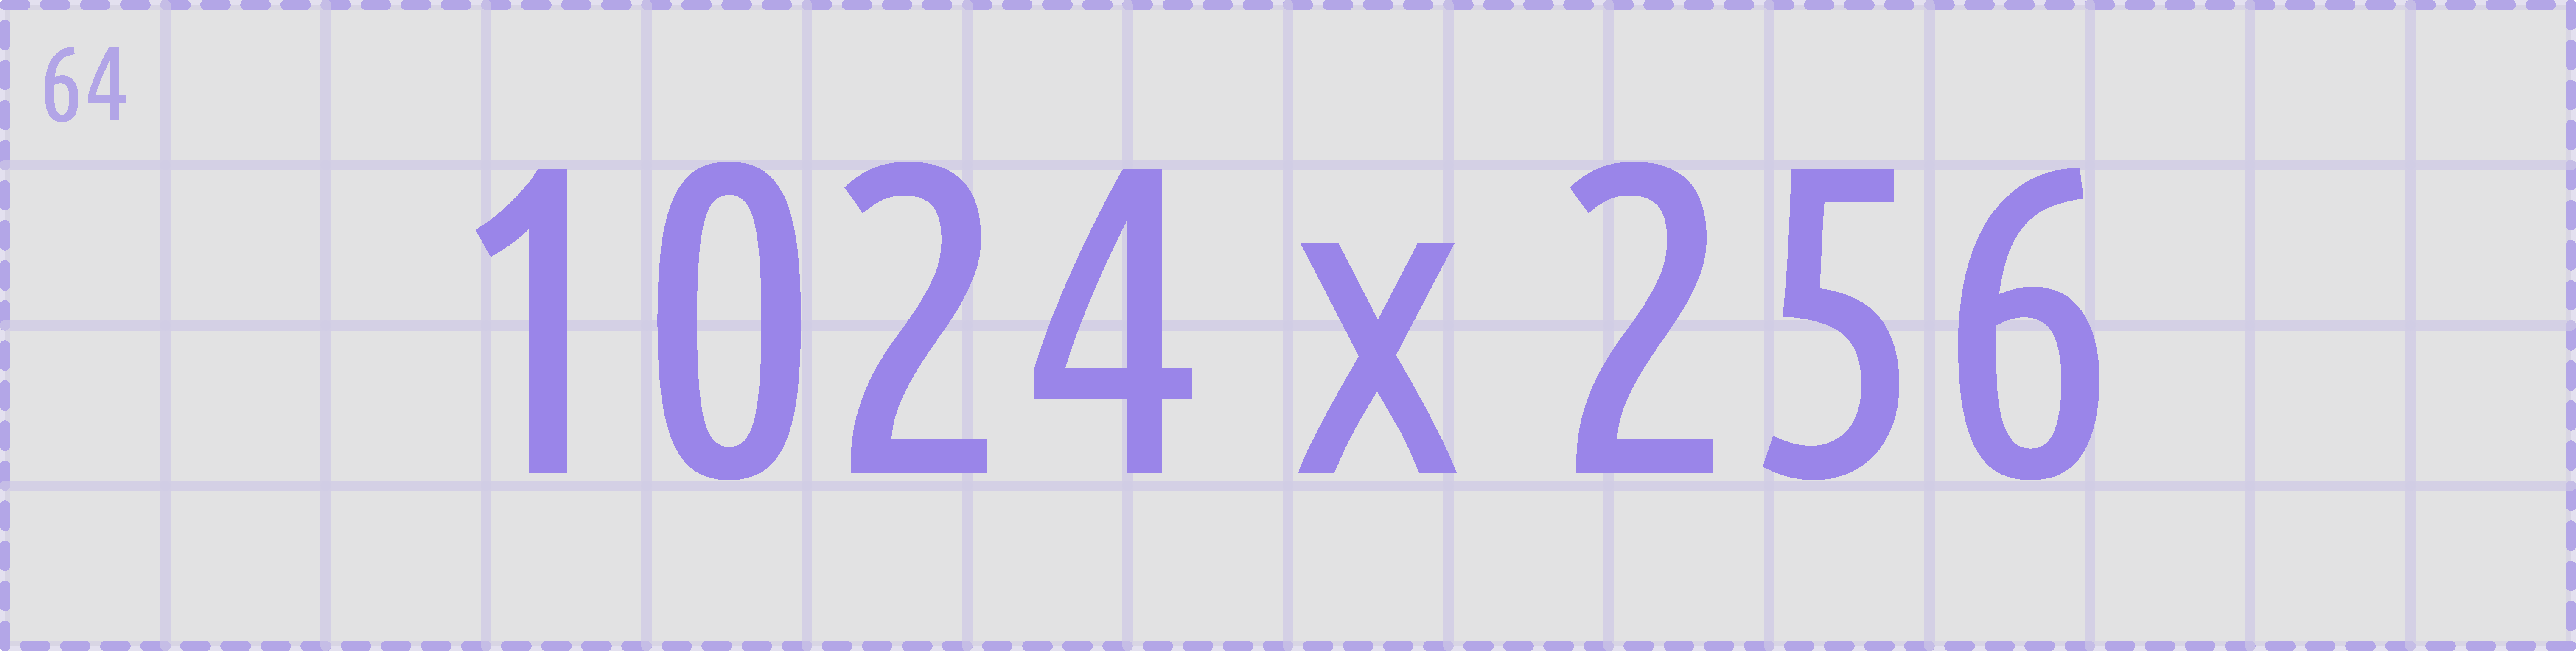
\includegraphics[width = 0.99\textwidth]{fig_1024x256.pdf}
  \vspace{-0.5cm}
  \caption{Comparison of the (nonlinear) mechanical compliance between the proposed hyper-elastic model \data{Matlab2} and the finite element simulations \data{Matlab1}. Notice the proposed stiffness model \eqref{eq:C2:stiffness_tanh_beta} does not capture the self-collision. }
  \vspace{-0.1cm}
  \label{fig:C2:fem_stress}
\end{figure}
%
\begin{align}
\q^\star & = \underset{\q}{\textrm{argmin}}\;  \left \lVert \log_{\SE{3}}\left[ \gB\inv(L,\q)\,\gB_L^{\textrm{FEM}}(\vec{u}) \right] \right \rVert_2,
\label{eq:C2:optimization_problem}
\end{align}
%
where $\gB_L^{\textrm{FEM}}$ is simply the corresponding end-effector configuration derived from the high-resolution finite element simulation given the input $\uB$. To some extent, \eqref{eq:C2:optimization_problem} can be viewed as an inverse kinematics optimization problem.
\vfill

\begin{rmk} Although straightforward for constant curvature soft-links, the approach could be easily extended to non-constant curvature and multi-link cases. However, an additional term $\Uf^\star = \tfrac{1}{2} \q^\top\mat{K}\q$ with some positive definite matrix $\mat{K} \succ 0 $ is required to ensure the nonlinear regression inhibits over-fitting.
\end{rmk}

Following the PCC condition, the bending angle $\beta$ can be calculated straightforwardly. Given these geometric curve parameters and the effective areas of the bellows, the applied elongation force and bending torque can be computed accordingly.

The numerical results are provided in Figure \ref{fig:C2:fem_stress}. In practice, these nonlinear strain relations can also be determined experimentally; however, the numerical methods have the beneficial convenience of several post-processing procedures and gravitation-free deformations. To support our previous claim concerning the consistency of the PCC condition, Figure \ref{fig:C2:fem_analysis} provides a few FEM snapshots results together with the optimal backbone curve from \eqref{eq:C2:pos_exact}. It can be seen that the piece-wise constant curvature (PCC) condition, although a clear oversimplification of the true mechanics at hand, is remarkably consistent with the FEM simulations.
%w
\begin{table}[!t]
\caption{Estimated hyper-elastic and visco-elastic material parameters for the study case soft robot \label{tab:C2:elastic_parameters}}
\centering
\begin{tabular}{ccccccc}
\hline
& $i=1$ &  $i=2$ &  $i=3$ & $i=4$ &  $i=5$ & $i=6$ \\
\hline
\hline
$\alpha$ &  \small{2.23}$\pwr{+3}$  & \small{1.74}$\pwr{+3}$  &  \small{-4.55}$\pwr{+2}$ & \small{1.31}$\pwr{-3}$  & \small{1.23}$\pwr{-2}$ & \small{-2.29}$\pwr{-1}$ \\[0.15em]
 $\alpha_\lambda$ &  \small{3.21}$\pwr{+2}$ & \small{5.22}$\pwr{-1}$ &  \small{26.4}$\pwr{+1}$& \small{1.82}$\pwr{-4}$ & \small{26.4}$\pwr{+1}$ & \small{1.82}$\pwr{-4}$ \\
\hline
\end{tabular}
\vspace{-3mm}
\end{table}
%
\subsection{Hyper-elasticity on joint space}
\noindent From the finite element results in Figure \ref{fig:C2:fem_analysis}, the mathematical description for the nonlinear stiffness can be detailed further. However, a suitable candidate function must be chosen first to properly represent the hyper-elastic stress-strain relation. The stiffness function $k_e (\varepsilon)$ and $k_b (\beta)$  have to satisfy the following properties.
%
\begin{asm}[Elastic boundedness]
\label{asm:C2:elastic_boundedness}
There exists positive constants ${k}^{-}$ and ${k}^{+}$ such that ${k}^{-} \le k_e(\xi),k_b(\xi) \le {k}^{+}$ for all possible strains $\xi \in \R$.
\end{asm}
%
\begin{asm}[Deformations reversibility]
\label{asm:C2:elastic_reversibility}
The stiffness functions $k_e(\xi)$ and $k_b(\xi)$ must have a global optimum (i.e., either a maximum or minimum) at their origin. As a result, the force produced by any deformation, given by ${\Ft} = \int_0^\xi k(s)s\;ds$, must be a monotonically increasing function where $\Ft = 0$ for the origin.
\end{asm}
%
Assumption \ref{asm:C2:elastic_boundedness} and \ref{asm:C2:elastic_reversibility} are necessary since they inhibit any elasto-plastic behavior, \ie, elastic bodies undergoing non-reversible deformation due to applied forces. Then. consider the following elasticity models for the nonlinear (hyper-elastic) elongation and bending stiffness:
%
\begin{align}
\label{eq:C2:stiffness_tanh_eps}
{k}_e(\q) & = \alpha_1 + \alpha_2 \left( \tanh[\alpha_3\,\varepsilon]^2 - 1 \right), \\[0.5em]
\label{eq:C2:stiffness_tanh_beta}
{k}_b(\q)  & = \alpha_{\phi}(\q) \cdot \left[\alpha_4 + \alpha_5 \left( \tanh[\alpha_6\,\beta]^2 - 1 \right)\right],
\end{align}
%
where $\vec{\alpha} = \left(\alpha_1,\,\alpha_2,\,\alpha_3,\alpha_4,\,\alpha_5,\,\alpha_6 \right)^\top$ is a vector composed of the (possibly time-varying) stiffness parameters, and $\alpha_\phi: \mathcal{Q} \to [1,\infty)$ a nonlinear correction term for asymmetry along the circumference of the radial-axis. Please note that these nonlinear functions possess a decomposable structure: a linear term and a nonlinear term that mimics strain-hardening or strain-softening. As for the asymmetric stiffness due to the layout of the pneumatic bellows, we propose the following ansatz:
%
\begin{asm}[Stiffness variation under radial offset]
Given the radial layout of the pneumatic bellows of the soft robot (see Figure \ref{fig:C2:soft_robot}), we assume that the nonlinear correction term for asymmetric radial stiffness along the circumference can be modeled by:
%
\begin{equation}
\alpha_\phi (\q) = \frac{1}{2}\beta \left[\sin( m \,\phi) + 1 \right] + 1,
\end{equation}
%
where $m$ is the number of bellows, and $\phi = \text{atan2}(\kappa_y,\kappa_x)$ the direction angle or heading. This stiffness correction term ensures the nonlinear bending stiffness becomes larger between bellows -- as it causes simultaneous deformation of multiple bellows. Please note that $\alpha_\phi(\q) \ge 1$ for all $\q \in \mathcal{Q}$.
\end{asm}

\begin{figure}[!t]
 \vspace{-3mm}
  \centering
  % This file was created by matlab2tikz.
%
\begin{tikzpicture}

\begin{axis}[%
width=0.324\textwidth,
height=0.325\textwidth,
at={(0\textwidth,0\textwidth)},
scale only axis,
xmin=-3.77645049743461,
xmax=3.77645049743461,
xlabel style={font=\color{white!15!black}},
xlabel={$\kappa_x$ (1/m)},
ymin=-3.77645049743461,
ymax=3.77645049743461,
ylabel style={font=\color{white!15!black}},
ylabel={$\kappa_y$ (1/m)},
axis background/.style={fill=white},
xmajorgrids,
ymajorgrids,
ylabel style={yshift=-1.75pt}
]

\addplot[%
surf,
shader=interp, colormap={mymap}{[1pt] rgb(0pt)=(0.2,0.1059,0.2431); rgb(1pt)=(0.2104,0.1627,0.3554); rgb(2pt)=(0.2202,0.204,0.4359); rgb(3pt)=(0.2295,0.2376,0.5013); rgb(4pt)=(0.2385,0.2666,0.5573); rgb(5pt)=(0.2471,0.2923,0.6069); rgb(6pt)=(0.2553,0.3156,0.6518); rgb(7pt)=(0.2633,0.337,0.6931); rgb(8pt)=(0.271,0.3569,0.7314); rgb(9pt)=(0.2784,0.3755,0.7672); rgb(10pt)=(0.2856,0.3931,0.801); rgb(11pt)=(0.2926,0.4097,0.833); rgb(12pt)=(0.2994,0.4256,0.8634); rgb(13pt)=(0.2993,0.4519,0.8765); rgb(14pt)=(0.295,0.4827,0.8798); rgb(15pt)=(0.2906,0.5111,0.883); rgb(16pt)=(0.2862,0.5377,0.8862); rgb(17pt)=(0.2817,0.5627,0.8894); rgb(18pt)=(0.277,0.5864,0.8926); rgb(19pt)=(0.2723,0.6089,0.8958); rgb(20pt)=(0.2675,0.6304,0.8989); rgb(21pt)=(0.2626,0.651,0.9021); rgb(22pt)=(0.2576,0.6707,0.9052); rgb(23pt)=(0.2524,0.6898,0.9083); rgb(24pt)=(0.2472,0.7082,0.9114); rgb(25pt)=(0.2441,0.7264,0.9089); rgb(26pt)=(0.2479,0.7455,0.8894); rgb(27pt)=(0.2516,0.764,0.8693); rgb(28pt)=(0.2553,0.782,0.8485); rgb(29pt)=(0.2589,0.7994,0.8271); rgb(30pt)=(0.2624,0.8163,0.8049); rgb(31pt)=(0.2659,0.8328,0.7819); rgb(32pt)=(0.2694,0.8488,0.7579); rgb(33pt)=(0.2728,0.8645,0.733); rgb(34pt)=(0.2761,0.8798,0.7068); rgb(35pt)=(0.2794,0.8947,0.6794); rgb(36pt)=(0.2827,0.9094,0.6504); rgb(37pt)=(0.2859,0.9237,0.6196); rgb(38pt)=(0.3296,0.9295,0.5999); rgb(39pt)=(0.3722,0.9341,0.5812); rgb(40pt)=(0.4095,0.9386,0.5616); rgb(41pt)=(0.4431,0.9431,0.5412); rgb(42pt)=(0.4737,0.9476,0.5197); rgb(43pt)=(0.5021,0.9521,0.4971); rgb(44pt)=(0.5285,0.9565,0.4731); rgb(45pt)=(0.5534,0.9609,0.4474); rgb(46pt)=(0.5769,0.9653,0.4198); rgb(47pt)=(0.5993,0.9696,0.3897); rgb(48pt)=(0.6206,0.974,0.3564); rgb(49pt)=(0.6411,0.9783,0.3189); rgb(50pt)=(0.6653,0.9741,0.2979); rgb(51pt)=(0.6928,0.9612,0.2976); rgb(52pt)=(0.7189,0.9482,0.2973); rgb(53pt)=(0.7438,0.9349,0.2969); rgb(54pt)=(0.7677,0.9214,0.2966); rgb(55pt)=(0.7907,0.9075,0.2963); rgb(56pt)=(0.8128,0.8934,0.296); rgb(57pt)=(0.8342,0.879,0.2957); rgb(58pt)=(0.8549,0.8643,0.2954); rgb(59pt)=(0.8749,0.8493,0.295); rgb(60pt)=(0.8944,0.8339,0.2947); rgb(61pt)=(0.9133,0.8181,0.2944); rgb(62pt)=(0.9299,0.8016,0.2934); rgb(63pt)=(0.9342,0.7825,0.2875); rgb(64pt)=(0.9384,0.7628,0.2815); rgb(65pt)=(0.9426,0.7424,0.2753); rgb(66pt)=(0.9468,0.7213,0.2689); rgb(67pt)=(0.951,0.6993,0.2624); rgb(68pt)=(0.9551,0.6764,0.2556); rgb(69pt)=(0.9592,0.6525,0.2487); rgb(70pt)=(0.9633,0.6273,0.2415); rgb(71pt)=(0.9673,0.6008,0.2341); rgb(72pt)=(0.9714,0.5726,0.2264); rgb(73pt)=(0.9754,0.5426,0.2183); rgb(74pt)=(0.9794,0.5103,0.21); rgb(75pt)=(0.9712,0.4904,0.204); rgb(76pt)=(0.9589,0.4744,0.1987); rgb(77pt)=(0.9463,0.4577,0.1933); rgb(78pt)=(0.9335,0.4402,0.1878); rgb(79pt)=(0.9205,0.4218,0.182); rgb(80pt)=(0.9072,0.4024,0.176); rgb(81pt)=(0.8936,0.3817,0.1699); rgb(82pt)=(0.8798,0.3596,0.1634); rgb(83pt)=(0.8657,0.3357,0.1567); rgb(84pt)=(0.8513,0.3095,0.1497); rgb(85pt)=(0.8365,0.2803,0.1423); rgb(86pt)=(0.8214,0.247,0.1345); rgb(87pt)=(0.8039,0.2207,0.1277); rgb(88pt)=(0.7824,0.2131,0.1232); rgb(89pt)=(0.76,0.2051,0.1185); rgb(90pt)=(0.7368,0.1967,0.1136); rgb(91pt)=(0.7126,0.188,0.1084); rgb(92pt)=(0.6873,0.1787,0.1031); rgb(93pt)=(0.6607,0.169,0.0975); rgb(94pt)=(0.6327,0.1586,0.0915); rgb(95pt)=(0.603,0.1474,0.0853); rgb(96pt)=(0.5712,0.1353,0.0786); rgb(97pt)=(0.537,0.122,0.0714); rgb(98pt)=(0.4999,0.1072,0.0635); rgb(99pt)=(0.4588,0.0902,0.0549)}, mesh/rows=50]
table[row sep=crcr, point meta=\thisrow{c}] {%
%
x	y	c\\
0	0	100\\
0.0641141357875468	0	100.000036708885\\
0.128228271575094	0	100.000146835527\\
0.19234240736264	0	100.000330379891\\
0.256456543150187	0	100.000587341917\\
0.320570678937734	0	100.00091772152\\
0.384684814725281	0	100.001321518594\\
0.448798950512828	0	100.001798733005\\
0.512913086300374	0	100.0023493646\\
0.577027222087921	0	100.002973413197\\
0.641141357875468	0	100.003670878594\\
0.705255493663015	0	100.004441760562\\
0.769369629450562	0	100.005286058851\\
0.833483765238108	0	100.006203773184\\
0.897597901025655	0	100.007194903263\\
0.961712036813202	0	100.008259448763\\
1.02582617260075	0	100.009397409337\\
1.0899403083883	0	100.010608784615\\
1.15405444417584	0	100.011893574201\\
1.21816857996339	0	100.013251777676\\
1.28228271575094	0	100.014683394596\\
1.34639685153848	0	100.016188424494\\
1.41051098732603	0	100.017766866879\\
1.47462512311358	0	100.019418721237\\
1.53873925890112	0	100.021143987028\\
1.60285339468867	0	100.02294266369\\
1.66696753047622	0	100.024814750635\\
1.73108166626376	0	100.026760247252\\
1.79519580205131	0	100.028779152908\\
1.85930993783886	0	100.030871466942\\
1.9234240736264	0	100.033037188673\\
1.98753820941395	0	100.035276317393\\
2.0516523452015	0	100.037588852373\\
2.11576648098904	0	100.039974792857\\
2.17988061677659	0	100.042434138068\\
2.24399475256414	0	100.044966887202\\
2.30810888835168	0	100.047573039433\\
2.37222302413923	0	100.050252593912\\
2.43633715992678	0	100.053005549763\\
2.50045129571433	0	100.055831906088\\
2.56456543150187	0	100.058731661966\\
2.62867956728942	0	100.061704816451\\
2.69279370307697	0	100.064751368571\\
2.75690783886451	0	100.067871317334\\
2.82102197465206	0	100.071064661721\\
2.88513611043961	0	100.07433140069\\
2.94925024622715	0	100.077671533176\\
3.0133643820147	0	100.081085058089\\
3.07747851780225	0	100.084571974315\\
3.14159265358979	0	100.088132280716\\
0	0	100\\
0.0635877596189965	0.00819873370836649	100.000036708885\\
0.127175519237993	0.016397467416733	100.000146835527\\
0.19076327885699	0.0245962011250995	100.000330379891\\
0.254351038475986	0.032794934833466	100.000587341917\\
0.317938798094983	0.0409936685418325	100.00091772152\\
0.381526557713979	0.049192402250199	100.001321518594\\
0.445114317332976	0.0573911359585655	100.001798733005\\
0.508702076951972	0.0655898696669319	100.0023493646\\
0.572289836570969	0.0737886033752985	100.002973413197\\
0.635877596189965	0.0819873370836649	100.003670878594\\
0.699465355808962	0.0901860707920314	100.004441760562\\
0.763053115427958	0.0983848045003979	100.005286058851\\
0.826640875046955	0.106583538208764	100.006203773184\\
0.890228634665951	0.114782271917131	100.007194903263\\
0.953816394284948	0.122981005625497	100.008259448763\\
1.01740415390394	0.131179739333864	100.009397409337\\
1.08099191352294	0.13937847304223	100.010608784615\\
1.14457967314194	0.147577206750597	100.011893574201\\
1.20816743276093	0.155775940458963	100.013251777676\\
1.27175519237993	0.16397467416733	100.014683394596\\
1.33534295199893	0.172173407875696	100.016188424494\\
1.39893071161792	0.180372141584063	100.017766866879\\
1.46251847123692	0.188570875292429	100.019418721237\\
1.52610623085592	0.196769609000796	100.021143987028\\
1.58969399047491	0.204968342709162	100.02294266369\\
1.65328175009391	0.213167076417529	100.024814750635\\
1.71686950971291	0.221365810125895	100.026760247252\\
1.7804572693319	0.229564543834262	100.028779152908\\
1.8440450289509	0.237763277542628	100.030871466942\\
1.9076327885699	0.245962011250995	100.033037188673\\
1.97122054818889	0.254160744959361	100.035276317393\\
2.03480830780789	0.262359478667728	100.037588852373\\
2.09839606742689	0.270558212376094	100.039974792857\\
2.16198382704588	0.278756946084461	100.042434138068\\
2.22557158666488	0.286955679792827	100.044966887202\\
2.28915934628388	0.295154413501194	100.047573039433\\
2.35274710590287	0.30335314720956	100.050252593912\\
2.41633486552187	0.311551880917927	100.053005549763\\
2.47992262514086	0.319750614626293	100.055831906088\\
2.54351038475986	0.32794934833466	100.058731661966\\
2.60709814437886	0.336148082043026	100.061704816451\\
2.67068590399785	0.344346815751393	100.064751368571\\
2.73427366361685	0.352545549459759	100.067871317334\\
2.79786142323585	0.360744283168126	100.071064661721\\
2.86144918285484	0.368943016876492	100.07433140069\\
2.92503694247384	0.377141750584859	100.077671533176\\
2.98862470209284	0.385340484293225	100.081085058089\\
3.05221246171183	0.393539218001592	100.084571974315\\
3.11580022133083	0.401737951709958	100.088132280716\\
0	0	100\\
0.0620172741954808	0.0162628444359078	100.000036708885\\
0.124034548390962	0.0325256888718157	100.000146835527\\
0.186051822586442	0.0487885333077235	100.000330379891\\
0.248069096781923	0.0650513777436313	100.000587341917\\
0.310086370977404	0.0813142221795392	100.00091772152\\
0.372103645172885	0.097577066615447	100.001321518594\\
0.434120919368366	0.113839911051355	100.001798733005\\
0.496138193563847	0.130102755487263	100.0023493646\\
0.558155467759327	0.146365599923171	100.002973413197\\
0.620172741954808	0.162628444359078	100.003670878594\\
0.682190016150289	0.178891288794986	100.004441760562\\
0.74420729034577	0.195154133230894	100.005286058851\\
0.806224564541251	0.211416977666802	100.006203773184\\
0.868241838736731	0.22767982210271	100.007194903263\\
0.930259112932212	0.243942666538618	100.008259448763\\
0.992276387127693	0.260205510974525	100.009397409337\\
1.05429366132317	0.276468355410433	100.010608784615\\
1.11631093551865	0.292731199846341	100.011893574201\\
1.17832820971414	0.308994044282249	100.013251777676\\
1.24034548390962	0.325256888718157	100.014683394596\\
1.3023627581051	0.341519733154065	100.016188424494\\
1.36438003230058	0.357782577589972	100.017766866879\\
1.42639730649606	0.37404542202588	100.019418721237\\
1.48841458069154	0.390308266461788	100.021143987028\\
1.55043185488702	0.406571110897696	100.02294266369\\
1.6124491290825	0.422833955333604	100.024814750635\\
1.67446640327798	0.439096799769512	100.026760247252\\
1.73648367747346	0.455359644205419	100.028779152908\\
1.79850095166894	0.471622488641327	100.030871466942\\
1.86051822586442	0.487885333077235	100.033037188673\\
1.92253550005991	0.504148177513143	100.035276317393\\
1.98455277425539	0.520411021949051	100.037588852373\\
2.04657004845087	0.536673866384959	100.039974792857\\
2.10858732264635	0.552936710820866	100.042434138068\\
2.17060459684183	0.569199555256774	100.044966887202\\
2.23262187103731	0.585462399692682	100.047573039433\\
2.29463914523279	0.60172524412859	100.050252593912\\
2.35665641942827	0.617988088564498	100.053005549763\\
2.41867369362375	0.634250933000406	100.055831906088\\
2.48069096781923	0.650513777436314	100.058731661966\\
2.54270824201471	0.666776621872221	100.061704816451\\
2.60472551621019	0.683039466308129	100.064751368571\\
2.66674279040567	0.699302310744037	100.067871317334\\
2.72876006460116	0.715565155179945	100.071064661721\\
2.79077733879664	0.731827999615853	100.07433140069\\
2.85279461299212	0.748090844051761	100.077671533176\\
2.9148118871876	0.764353688487668	100.081085058089\\
2.97682916138308	0.780616532923576	100.084571974315\\
3.03884643557856	0.796879377359484	100.088132280716\\
0	0	100\\
0.0594284668442354	0.0240599197074222	100.000036708885\\
0.118856933688471	0.0481198394148444	100.000146835527\\
0.178285400532706	0.0721797591222665	100.000330379891\\
0.237713867376942	0.0962396788296887	100.000587341917\\
0.297142334221177	0.120299598537111	100.00091772152\\
0.356570801065412	0.144359518244533	100.001321518594\\
0.415999267909648	0.168419437951955	100.001798733005\\
0.475427734753883	0.192479357659377	100.0023493646\\
0.534856201598119	0.2165392773668	100.002973413197\\
0.594284668442354	0.240599197074222	100.003670878594\\
0.653713135286589	0.264659116781644	100.004441760562\\
0.713141602130825	0.288719036489066	100.005286058851\\
0.77257006897506	0.312778956196488	100.006203773184\\
0.831998535819296	0.33683887590391	100.007194903263\\
0.891427002663531	0.360898795611333	100.008259448763\\
0.950855469507766	0.384958715318755	100.009397409337\\
1.010283936352	0.409018635026177	100.010608784615\\
1.06971240319624	0.433078554733599	100.011893574201\\
1.12914087004047	0.457138474441021	100.013251777676\\
1.18856933688471	0.481198394148444	100.014683394596\\
1.24799780372894	0.505258313855866	100.016188424494\\
1.30742627057318	0.529318233563288	100.017766866879\\
1.36685473741741	0.55337815327071	100.019418721237\\
1.42628320426165	0.577438072978132	100.021143987028\\
1.48571167110589	0.601497992685554	100.02294266369\\
1.54514013795012	0.625557912392977	100.024814750635\\
1.60456860479436	0.649617832100399	100.026760247252\\
1.66399707163859	0.673677751807821	100.028779152908\\
1.72342553848283	0.697737671515243	100.030871466942\\
1.78285400532706	0.721797591222665	100.033037188673\\
1.8422824721713	0.745857510930087	100.035276317393\\
1.90171093901553	0.76991743063751	100.037588852373\\
1.96113940585977	0.793977350344932	100.039974792857\\
2.020567872704	0.818037270052354	100.042434138068\\
2.07999633954824	0.842097189759776	100.044966887202\\
2.13942480639247	0.866157109467198	100.047573039433\\
2.19885327323671	0.890217029174621	100.050252593912\\
2.25828174008095	0.914276948882043	100.053005549763\\
2.31771020692518	0.938336868589465	100.055831906088\\
2.37713867376942	0.962396788296887	100.058731661966\\
2.43656714061365	0.986456708004309	100.061704816451\\
2.49599560745789	1.01051662771173	100.064751368571\\
2.55542407430212	1.03457654741915	100.067871317334\\
2.61485254114636	1.05863646712658	100.071064661721\\
2.67428100799059	1.082696386834	100.07433140069\\
2.73370947483483	1.10675630654142	100.077671533176\\
2.79313794167906	1.13081622624884	100.081085058089\\
2.8525664085233	1.15487614595626	100.084571974315\\
2.91199487536753	1.17893606566369	100.088132280716\\
0	0	100\\
0.0558638457103963	0.031461931762513	100.000036708885\\
0.111727691420793	0.062923863525026	100.000146835527\\
0.167591537131189	0.0943857952875391	100.000330379891\\
0.223455382841585	0.125847727050052	100.000587341917\\
0.279319228551981	0.157309658812565	100.00091772152\\
0.335183074262378	0.188771590575078	100.001321518594\\
0.391046919972774	0.220233522337591	100.001798733005\\
0.44691076568317	0.251695454100104	100.0023493646\\
0.502774611393567	0.283157385862617	100.002973413197\\
0.558638457103963	0.31461931762513	100.003670878594\\
0.614502302814359	0.346081249387643	100.004441760562\\
0.670366148524756	0.377543181150156	100.005286058851\\
0.726229994235152	0.409005112912669	100.006203773184\\
0.782093839945548	0.440467044675182	100.007194903263\\
0.837957685655945	0.471928976437695	100.008259448763\\
0.893821531366341	0.503390908200208	100.009397409337\\
0.949685377076737	0.534852839962722	100.010608784615\\
1.00554922278713	0.566314771725235	100.011893574201\\
1.06141306849753	0.597776703487747	100.013251777676\\
1.11727691420793	0.629238635250261	100.014683394596\\
1.17314075991832	0.660700567012774	100.016188424494\\
1.22900460562872	0.692162498775286	100.017766866879\\
1.28486845133911	0.7236244305378	100.019418721237\\
1.34073229704951	0.755086362300313	100.021143987028\\
1.39659614275991	0.786548294062826	100.02294266369\\
1.4524599884703	0.818010225825339	100.024814750635\\
1.5083238341807	0.849472157587852	100.026760247252\\
1.5641876798911	0.880934089350365	100.028779152908\\
1.62005152560149	0.912396021112878	100.030871466942\\
1.67591537131189	0.943857952875391	100.033037188673\\
1.73177921702229	0.975319884637904	100.035276317393\\
1.78764306273268	1.00678181640042	100.037588852373\\
1.84350690844308	1.03824374816293	100.039974792857\\
1.89937075415347	1.06970567992544	100.042434138068\\
1.95523459986387	1.10116761168796	100.044966887202\\
2.01109844557427	1.13262954345047	100.047573039433\\
2.06696229128466	1.16409147521298	100.050252593912\\
2.12282613699506	1.19555340697549	100.053005549763\\
2.17868998270546	1.22701533873801	100.055831906088\\
2.23455382841585	1.25847727050052	100.058731661966\\
2.29041767412625	1.28993920226303	100.061704816451\\
2.34628151983664	1.32140113402555	100.064751368571\\
2.40214536554704	1.35286306578806	100.067871317334\\
2.45800921125744	1.38432499755057	100.071064661721\\
2.51387305696783	1.41578692931309	100.07433140069\\
2.56973690267823	1.4472488610756	100.077671533176\\
2.62560074838863	1.47871079283811	100.081085058089\\
2.68146459409902	1.51017272460063	100.084571974315\\
2.73732843980942	1.54163465636314	100.088132280716\\
0	0	100\\
0.0513819417744319	0.0383473397678755	100.000036708885\\
0.102763883548864	0.0766946795357509	100.000146835527\\
0.154145825323296	0.115042019303626	100.000330379891\\
0.205527767097727	0.153389359071502	100.000587341917\\
0.256909708872159	0.191736698839377	100.00091772152\\
0.308291650646591	0.230084038607253	100.001321518594\\
0.359673592421023	0.268431378375128	100.001798733005\\
0.411055534195455	0.306778718143004	100.0023493646\\
0.462437475969887	0.345126057910879	100.002973413197\\
0.513819417744319	0.383473397678755	100.003670878594\\
0.56520135951875	0.42182073744663	100.004441760562\\
0.616583301293182	0.460168077214506	100.005286058851\\
0.667965243067614	0.498515416982381	100.006203773184\\
0.719347184842046	0.536862756750257	100.007194903263\\
0.770729126616478	0.575210096518132	100.008259448763\\
0.82211106839091	0.613557436286007	100.009397409337\\
0.873493010165342	0.651904776053883	100.010608784615\\
0.924874951939773	0.690252115821758	100.011893574201\\
0.976256893714205	0.728599455589634	100.013251777676\\
1.02763883548864	0.766946795357509	100.014683394596\\
1.07902077726307	0.805294135125385	100.016188424494\\
1.1304027190375	0.84364147489326	100.017766866879\\
1.18178466081193	0.881988814661136	100.019418721237\\
1.23316660258636	0.920336154429011	100.021143987028\\
1.2845485443608	0.958683494196887	100.02294266369\\
1.33593048613523	0.997030833964762	100.024814750635\\
1.38731242790966	1.03537817373264	100.026760247252\\
1.43869436968409	1.07372551350051	100.028779152908\\
1.49007631145852	1.11207285326839	100.030871466942\\
1.54145825323296	1.15042019303626	100.033037188673\\
1.59284019500739	1.18876753280414	100.035276317393\\
1.64422213678182	1.22711487257201	100.037588852373\\
1.69560407855625	1.26546221233989	100.039974792857\\
1.74698602033068	1.30380955210777	100.042434138068\\
1.79836796210511	1.34215689187564	100.044966887202\\
1.84974990387955	1.38050423164352	100.047573039433\\
1.90113184565398	1.41885157141139	100.050252593912\\
1.95251378742841	1.45719891117927	100.053005549763\\
2.00389572920284	1.49554625094714	100.055831906088\\
2.05527767097727	1.53389359071502	100.058731661966\\
2.10665961275171	1.57224093048289	100.061704816451\\
2.15804155452614	1.61058827025077	100.064751368571\\
2.20942349630057	1.64893561001865	100.067871317334\\
2.260805438075	1.68728294978652	100.071064661721\\
2.31218737984943	1.7256302895544	100.07433140069\\
2.36356932162387	1.76397762932227	100.077671533176\\
2.4149512633983	1.80232496909015	100.081085058089\\
2.46633320517273	1.84067230885802	100.084571974315\\
2.51771514694716	1.8790196486259	100.088132280716\\
0	0	100\\
0.0460563477750617	0.0446030855144188	100.000036708885\\
0.0921126955501234	0.0892061710288376	100.000146835527\\
0.138169043325185	0.133809256543256	100.000330379891\\
0.184225391100247	0.178412342057675	100.000587341917\\
0.230281738875309	0.223015427572094	100.00091772152\\
0.27633808665037	0.267618513086513	100.001321518594\\
0.322394434425432	0.312221598600932	100.001798733005\\
0.368450782200494	0.356824684115351	100.0023493646\\
0.414507129975555	0.401427769629769	100.002973413197\\
0.460563477750617	0.446030855144188	100.003670878594\\
0.506619825525679	0.490633940658607	100.004441760562\\
0.55267617330074	0.535237026173026	100.005286058851\\
0.598732521075802	0.579840111687445	100.006203773184\\
0.644788868850864	0.624443197201863	100.007194903263\\
0.690845216625925	0.669046282716282	100.008259448763\\
0.736901564400987	0.713649368230701	100.009397409337\\
0.782957912176049	0.75825245374512	100.010608784615\\
0.829014259951111	0.802855539259539	100.011893574201\\
0.875070607726172	0.847458624773958	100.013251777676\\
0.921126955501234	0.892061710288376	100.014683394596\\
0.967183303276296	0.936664795802795	100.016188424494\\
1.01323965105136	0.981267881317214	100.017766866879\\
1.05929599882642	1.02587096683163	100.019418721237\\
1.10535234660148	1.07047405234605	100.021143987028\\
1.15140869437654	1.11507713786047	100.02294266369\\
1.1974650421516	1.15968022337489	100.024814750635\\
1.24352138992667	1.20428330888931	100.026760247252\\
1.28957773770173	1.24888639440373	100.028779152908\\
1.33563408547679	1.29348947991815	100.030871466942\\
1.38169043325185	1.33809256543256	100.033037188673\\
1.42774678102691	1.38269565094698	100.035276317393\\
1.47380312880197	1.4272987364614	100.037588852373\\
1.51985947657704	1.47190182197582	100.039974792857\\
1.5659158243521	1.51650490749024	100.042434138068\\
1.61197217212716	1.56110799300466	100.044966887202\\
1.65802851990222	1.60571107851908	100.047573039433\\
1.70408486767728	1.6503141640335	100.050252593912\\
1.75014121545234	1.69491724954792	100.053005549763\\
1.79619756322741	1.73952033506233	100.055831906088\\
1.84225391100247	1.78412342057675	100.058731661966\\
1.88831025877753	1.82872650609117	100.061704816451\\
1.93436660655259	1.87332959160559	100.064751368571\\
1.98042295432765	1.91793267712001	100.067871317334\\
2.02647930210271	1.96253576263443	100.071064661721\\
2.07253564987778	2.00713884814885	100.07433140069\\
2.11859199765284	2.05174193366327	100.077671533176\\
2.1646483454279	2.09634501917768	100.081085058089\\
2.21070469320296	2.1409481046921	100.084571974315\\
2.25676104097802	2.18555119020652	100.088132280716\\
0	0	100\\
0.0399745098185215	0.0501264498299343	100.000036708885\\
0.079949019637043	0.100252899659869	100.000146835527\\
0.119923529455564	0.150379349489803	100.000330379891\\
0.159898039274086	0.200505799319737	100.000587341917\\
0.199872549092607	0.250632249149671	100.00091772152\\
0.239847058911129	0.300758698979606	100.001321518594\\
0.27982156872965	0.35088514880954	100.001798733005\\
0.319796078548172	0.401011598639474	100.0023493646\\
0.359770588366693	0.451138048469409	100.002973413197\\
0.399745098185215	0.501264498299343	100.003670878594\\
0.439719608003736	0.551390948129277	100.004441760562\\
0.479694117822258	0.601517397959211	100.005286058851\\
0.519668627640779	0.651643847789146	100.006203773184\\
0.559643137459301	0.70177029761908	100.007194903263\\
0.599617647277822	0.751896747449014	100.008259448763\\
0.639592157096344	0.802023197278948	100.009397409337\\
0.679566666914865	0.852149647108883	100.010608784615\\
0.719541176733387	0.902276096938817	100.011893574201\\
0.759515686551908	0.952402546768751	100.013251777676\\
0.79949019637043	1.00252899659869	100.014683394596\\
0.839464706188951	1.05265544642862	100.016188424494\\
0.879439216007473	1.10278189625855	100.017766866879\\
0.919413725825994	1.15290834608849	100.019418721237\\
0.959388235644516	1.20303479591842	100.021143987028\\
0.999362745463037	1.25316124574836	100.02294266369\\
1.03933725528156	1.30328769557829	100.024814750635\\
1.07931176510008	1.35341414540823	100.026760247252\\
1.1192862749186	1.40354059523816	100.028779152908\\
1.15926078473712	1.45366704506809	100.030871466942\\
1.19923529455564	1.50379349489803	100.033037188673\\
1.23920980437417	1.55391994472796	100.035276317393\\
1.27918431419269	1.6040463945579	100.037588852373\\
1.31915882401121	1.65417284438783	100.039974792857\\
1.35913333382973	1.70429929421777	100.042434138068\\
1.39910784364825	1.7544257440477	100.044966887202\\
1.43908235346677	1.80455219387763	100.047573039433\\
1.4790568632853	1.85467864370757	100.050252593912\\
1.51903137310382	1.9048050935375	100.053005549763\\
1.55900588292234	1.95493154336744	100.055831906088\\
1.59898039274086	2.00505799319737	100.058731661966\\
1.63895490255938	2.05518444302731	100.061704816451\\
1.6789294123779	2.10531089285724	100.064751368571\\
1.71890392219642	2.15543734268717	100.067871317334\\
1.75887843201495	2.20556379251711	100.071064661721\\
1.79885294183347	2.25569024234704	100.07433140069\\
1.83882745165199	2.30581669217698	100.077671533176\\
1.87880196147051	2.35594314200691	100.081085058089\\
1.91877647128903	2.40606959183685	100.084571974315\\
1.95875098110755	2.45619604166678	100.088132280716\\
0	0	100\\
0.0332362915159161	0.0548267392250627	100.000036708885\\
0.0664725830318323	0.109653478450125	100.000146835527\\
0.0997088745477484	0.164480217675188	100.000330379891\\
0.132945166063665	0.219306956900251	100.000587341917\\
0.166181457579581	0.274133696125314	100.00091772152\\
0.199417749095497	0.328960435350376	100.001321518594\\
0.232654040611413	0.383787174575439	100.001798733005\\
0.265890332127329	0.438613913800502	100.0023493646\\
0.299126623643245	0.493440653025564	100.002973413197\\
0.332362915159161	0.548267392250627	100.003670878594\\
0.365599206675077	0.60309413147569	100.004441760562\\
0.398835498190994	0.657920870700752	100.005286058851\\
0.43207178970691	0.712747609925815	100.006203773184\\
0.465308081222826	0.767574349150878	100.007194903263\\
0.498544372738742	0.822401088375941	100.008259448763\\
0.531780664254658	0.877227827601003	100.009397409337\\
0.565016955770574	0.932054566826066	100.010608784615\\
0.598253247286491	0.986881306051129	100.011893574201\\
0.631489538802407	1.04170804527619	100.013251777676\\
0.664725830318323	1.09653478450125	100.014683394596\\
0.697962121834239	1.15136152372632	100.016188424494\\
0.731198413350155	1.20618826295138	100.017766866879\\
0.764434704866071	1.26101500217644	100.019418721237\\
0.797670996381987	1.3158417414015	100.021143987028\\
0.830907287897904	1.37066848062657	100.02294266369\\
0.86414357941382	1.42549521985163	100.024814750635\\
0.897379870929736	1.48032195907669	100.026760247252\\
0.930616162445652	1.53514869830176	100.028779152908\\
0.963852453961568	1.58997543752682	100.030871466942\\
0.997088745477484	1.64480217675188	100.033037188673\\
1.0303250369934	1.69962891597694	100.035276317393\\
1.06356132850932	1.75445565520201	100.037588852373\\
1.09679762002523	1.80928239442707	100.039974792857\\
1.13003391154115	1.86410913365213	100.042434138068\\
1.16327020305706	1.91893587287719	100.044966887202\\
1.19650649457298	1.97376261210226	100.047573039433\\
1.2297427860889	2.02858935132732	100.050252593912\\
1.26297907760481	2.08341609055238	100.053005549763\\
1.29621536912073	2.13824282977745	100.055831906088\\
1.32945166063665	2.19306956900251	100.058731661966\\
1.36268795215256	2.24789630822757	100.061704816451\\
1.39592424366848	2.30272304745263	100.064751368571\\
1.42916053518439	2.3575497866777	100.067871317334\\
1.46239682670031	2.41237652590276	100.071064661721\\
1.49563311821623	2.46720326512782	100.07433140069\\
1.52886940973214	2.52203000435288	100.077671533176\\
1.56210570124806	2.57685674357795	100.081085058089\\
1.59534199276397	2.63168348280301	100.084571974315\\
1.62857828427989	2.68651022202807	100.088132280716\\
0	0	100\\
0.0259523342254863	0.0586267750778826	100.000036708885\\
0.0519046684509726	0.117253550155765	100.000146835527\\
0.0778570026764589	0.175880325233648	100.000330379891\\
0.103809336901945	0.234507100311531	100.000587341917\\
0.129761671127432	0.293133875389413	100.00091772152\\
0.155714005352918	0.351760650467296	100.001321518594\\
0.181666339578404	0.410387425545178	100.001798733005\\
0.20761867380389	0.469014200623061	100.0023493646\\
0.233571008029377	0.527640975700944	100.002973413197\\
0.259523342254863	0.586267750778826	100.003670878594\\
0.285475676480349	0.644894525856709	100.004441760562\\
0.311428010705836	0.703521300934592	100.005286058851\\
0.337380344931322	0.762148076012474	100.006203773184\\
0.363332679156808	0.820774851090357	100.007194903263\\
0.389285013382295	0.87940162616824	100.008259448763\\
0.415237347607781	0.938028401246122	100.009397409337\\
0.441189681833267	0.996655176324005	100.010608784615\\
0.467142016058753	1.05528195140189	100.011893574201\\
0.49309435028424	1.11390872647977	100.013251777676\\
0.519046684509726	1.17253550155765	100.014683394596\\
0.544999018735212	1.23116227663554	100.016188424494\\
0.570951352960699	1.28978905171342	100.017766866879\\
0.596903687186185	1.3484158267913	100.019418721237\\
0.622856021411671	1.40704260186918	100.021143987028\\
0.648808355637158	1.46566937694707	100.02294266369\\
0.674760689862644	1.52429615202495	100.024814750635\\
0.70071302408813	1.58292292710283	100.026760247252\\
0.726665358313616	1.64154970218071	100.028779152908\\
0.752617692539103	1.7001764772586	100.030871466942\\
0.778570026764589	1.75880325233648	100.033037188673\\
0.804522360990075	1.81743002741436	100.035276317393\\
0.830474695215562	1.87605680249224	100.037588852373\\
0.856427029441048	1.93468357757013	100.039974792857\\
0.882379363666534	1.99331035264801	100.042434138068\\
0.908331697892021	2.05193712772589	100.044966887202\\
0.934284032117507	2.11056390280378	100.047573039433\\
0.960236366342993	2.16919067788166	100.050252593912\\
0.986188700568479	2.22781745295954	100.053005549763\\
1.01214103479397	2.28644422803742	100.055831906088\\
1.03809336901945	2.34507100311531	100.058731661966\\
1.06404570324494	2.40369777819319	100.061704816451\\
1.08999803747042	2.46232455327107	100.064751368571\\
1.11595037169591	2.52095132834895	100.067871317334\\
1.1419027059214	2.57957810342684	100.071064661721\\
1.16785504014688	2.63820487850472	100.07433140069\\
1.19380737437237	2.6968316535826	100.077671533176\\
1.21975970859786	2.75545842866048	100.081085058089\\
1.24571204282334	2.81408520373837	100.084571974315\\
1.27166437704883	2.87271197881625	100.088132280716\\
0	0	100\\
0.018242240324565	0.0614641609047484	100.000036708885\\
0.03648448064913	0.122928321809497	100.000146835527\\
0.054726720973695	0.184392482714245	100.000330379891\\
0.07296896129826	0.245856643618994	100.000587341917\\
0.091211201622825	0.307320804523742	100.00091772152\\
0.10945344194739	0.36878496542849	100.001321518594\\
0.127695682271955	0.430249126333239	100.001798733005\\
0.14593792259652	0.491713287237987	100.0023493646\\
0.164180162921085	0.553177448142736	100.002973413197\\
0.18242240324565	0.614641609047484	100.003670878594\\
0.200664643570215	0.676105769952232	100.004441760562\\
0.21890688389478	0.737569930856981	100.005286058851\\
0.237149124219345	0.799034091761729	100.006203773184\\
0.25539136454391	0.860498252666478	100.007194903263\\
0.273633604868475	0.921962413571226	100.008259448763\\
0.29187584519304	0.983426574475975	100.009397409337\\
0.310118085517605	1.04489073538072	100.010608784615\\
0.32836032584217	1.10635489628547	100.011893574201\\
0.346602566166735	1.16781905719022	100.013251777676\\
0.3648448064913	1.22928321809497	100.014683394596\\
0.383087046815865	1.29074737899972	100.016188424494\\
0.40132928714043	1.35221153990446	100.017766866879\\
0.419571527464995	1.41367570080921	100.019418721237\\
0.43781376778956	1.47513986171396	100.021143987028\\
0.456056008114125	1.53660402261871	100.02294266369\\
0.47429824843869	1.59806818352346	100.024814750635\\
0.492540488763255	1.65953234442821	100.026760247252\\
0.51078272908782	1.72099650533296	100.028779152908\\
0.529024969412385	1.7824606662377	100.030871466942\\
0.54726720973695	1.84392482714245	100.033037188673\\
0.565509450061515	1.9053889880472	100.035276317393\\
0.58375169038608	1.96685314895195	100.037588852373\\
0.601993930710645	2.0283173098567	100.039974792857\\
0.62023617103521	2.08978147076145	100.042434138068\\
0.638478411359775	2.15124563166619	100.044966887202\\
0.65672065168434	2.21270979257094	100.047573039433\\
0.674962892008905	2.27417395347569	100.050252593912\\
0.69320513233347	2.33563811438044	100.053005549763\\
0.711447372658035	2.39710227528519	100.055831906088\\
0.7296896129826	2.45856643618994	100.058731661966\\
0.747931853307165	2.52003059709469	100.061704816451\\
0.76617409363173	2.58149475799943	100.064751368571\\
0.784416333956295	2.64295891890418	100.067871317334\\
0.80265857428086	2.70442307980893	100.071064661721\\
0.820900814605425	2.76588724071368	100.07433140069\\
0.83914305492999	2.82735140161843	100.077671533176\\
0.857385295254555	2.88881556252318	100.081085058089\\
0.87562753557912	2.95027972342792	100.084571974315\\
0.893869775903685	3.01174388433267	100.088132280716\\
0	0	100\\
0.0102326093418483	0.0632923069088267	100.000036708885\\
0.0204652186836966	0.126584613817653	100.000146835527\\
0.0306978280255449	0.18987692072648	100.000330379891\\
0.0409304373673932	0.253169227635307	100.000587341917\\
0.0511630467092416	0.316461534544133	100.00091772152\\
0.0613956560510899	0.37975384145296	100.001321518594\\
0.0716282653929382	0.443046148361787	100.001798733005\\
0.0818608747347865	0.506338455270613	100.0023493646\\
0.0920934840766348	0.56963076217944	100.002973413197\\
0.102326093418483	0.632923069088267	100.003670878594\\
0.112558702760331	0.696215375997093	100.004441760562\\
0.12279131210218	0.75950768290592	100.005286058851\\
0.133023921444028	0.822799989814747	100.006203773184\\
0.143256530785876	0.886092296723573	100.007194903263\\
0.153489140127725	0.9493846036324	100.008259448763\\
0.163721749469573	1.01267691054123	100.009397409337\\
0.173954358811421	1.07596921745005	100.010608784615\\
0.18418696815327	1.13926152435888	100.011893574201\\
0.194419577495118	1.20255383126771	100.013251777676\\
0.204652186836966	1.26584613817653	100.014683394596\\
0.214884796178815	1.32913844508536	100.016188424494\\
0.225117405520663	1.39243075199419	100.017766866879\\
0.235350014862511	1.45572305890301	100.019418721237\\
0.245582624204359	1.51901536581184	100.021143987028\\
0.255815233546208	1.58230767272067	100.02294266369\\
0.266047842888056	1.64559997962949	100.024814750635\\
0.276280452229904	1.70889228653832	100.026760247252\\
0.286513061571753	1.77218459344715	100.028779152908\\
0.296745670913601	1.83547690035597	100.030871466942\\
0.306978280255449	1.8987692072648	100.033037188673\\
0.317210889597298	1.96206151417363	100.035276317393\\
0.327443498939146	2.02535382108245	100.037588852373\\
0.337676108280994	2.08864612799128	100.039974792857\\
0.347908717622843	2.15193843490011	100.042434138068\\
0.358141326964691	2.21523074180893	100.044966887202\\
0.368373936306539	2.27852304871776	100.047573039433\\
0.378606545648388	2.34181535562659	100.050252593912\\
0.388839154990236	2.40510766253541	100.053005549763\\
0.399071764332084	2.46839996944424	100.055831906088\\
0.409304373673932	2.53169227635307	100.058731661966\\
0.419536983015781	2.59498458326189	100.061704816451\\
0.429769592357629	2.65827689017072	100.064751368571\\
0.440002201699477	2.72156919707955	100.067871317334\\
0.450234811041326	2.78486150398837	100.071064661721\\
0.460467420383174	2.8481538108972	100.07433140069\\
0.470700029725022	2.91144611780603	100.077671533176\\
0.480932639066871	2.97473842471485	100.081085058089\\
0.491165248408719	3.03803073162368	100.084571974315\\
0.501397857750567	3.10132303853251	100.088132280716\\
0	0	100\\
0.0020549591966342	0.0640811949832722	100.000036708885\\
0.0041099183932684	0.128162389966544	100.000146835527\\
0.0061648775899026	0.192243584949817	100.000330379891\\
0.0082198367865368	0.256324779933089	100.000587341917\\
0.010274795983171	0.320405974916361	100.00091772152\\
0.0123297551798052	0.384487169899634	100.001321518594\\
0.0143847143764394	0.448568364882906	100.001798733005\\
0.0164396735730736	0.512649559866178	100.0023493646\\
0.0184946327697078	0.57673075484945	100.002973413197\\
0.020549591966342	0.640811949832723	100.003670878594\\
0.0226045511629762	0.704893144815995	100.004441760562\\
0.0246595103596104	0.768974339799267	100.005286058851\\
0.0267144695562446	0.833055534782539	100.006203773184\\
0.0287694287528788	0.897136729765812	100.007194903263\\
0.030824387949513	0.961217924749084	100.008259448763\\
0.0328793471461472	1.02529911973236	100.009397409337\\
0.0349343063427814	1.08938031471563	100.010608784615\\
0.0369892655394156	1.1534615096989	100.011893574201\\
0.0390442247360498	1.21754270468217	100.013251777676\\
0.041099183932684	1.28162389966545	100.014683394596\\
0.0431541431293182	1.34570509464872	100.016188424494\\
0.0452091023259524	1.40978628963199	100.017766866879\\
0.0472640615225866	1.47386748461526	100.019418721237\\
0.0493190207192208	1.53794867959853	100.021143987028\\
0.051373979915855	1.60202987458181	100.02294266369\\
0.0534289391124892	1.66611106956508	100.024814750635\\
0.0554838983091234	1.73019226454835	100.026760247252\\
0.0575388575057576	1.79427345953162	100.028779152908\\
0.0595938167023918	1.8583546545149	100.030871466942\\
0.061648775899026	1.92243584949817	100.033037188673\\
0.0637037350956602	1.98651704448144	100.035276317393\\
0.0657586942922944	2.05059823946471	100.037588852373\\
0.0678136534889286	2.11467943444798	100.039974792857\\
0.0698686126855628	2.17876062943126	100.042434138068\\
0.071923571882197	2.24284182441453	100.044966887202\\
0.0739785310788312	2.3069230193978	100.047573039433\\
0.0760334902754654	2.37100421438107	100.050252593912\\
0.0780884494720996	2.43508540936435	100.053005549763\\
0.0801434086687338	2.49916660434762	100.055831906088\\
0.082198367865368	2.56324779933089	100.058731661966\\
0.0842533270620022	2.62732899431416	100.061704816451\\
0.0863082862586364	2.69141018929743	100.064751368571\\
0.0883632454552706	2.75549138428071	100.067871317334\\
0.0904182046519048	2.81957257926398	100.071064661721\\
0.092473163848539	2.88365377424725	100.07433140069\\
0.0945281230451732	2.94773496923052	100.077671533176\\
0.0965830822418074	3.0118161642138	100.081085058089\\
0.0986380414384416	3.07589735919707	100.084571974315\\
0.100693000635076	3.13997855418034	100.088132280716\\
-0	0	100\\
-0.00615643332177623	0.0638178716077128	100.000036708885\\
-0.0123128666435525	0.127635743215426	100.000146835527\\
-0.0184692999653287	0.191453614823138	100.000330379891\\
-0.0246257332871049	0.255271486430851	100.000587341917\\
-0.0307821666088812	0.319089358038564	100.00091772152\\
-0.0369385999306574	0.382907229646277	100.001321518594\\
-0.0430950332524336	0.446725101253989	100.001798733005\\
-0.0492514665742099	0.510542972861702	100.0023493646\\
-0.0554078998959861	0.574360844469415	100.002973413197\\
-0.0615643332177623	0.638178716077128	100.003670878594\\
-0.0677207665395385	0.70199658768484	100.004441760562\\
-0.0738771998613148	0.765814459292553	100.005286058851\\
-0.080033633183091	0.829632330900266	100.006203773184\\
-0.0861900665048673	0.893450202507979	100.007194903263\\
-0.0923464998266435	0.957268074115692	100.008259448763\\
-0.0985029331484197	1.0210859457234	100.009397409337\\
-0.104659366470196	1.08490381733112	100.010608784615\\
-0.110815799791972	1.14872168893883	100.011893574201\\
-0.116972233113748	1.21253956054654	100.013251777676\\
-0.123128666435525	1.27635743215426	100.014683394596\\
-0.129285099757301	1.34017530376197	100.016188424494\\
-0.135441533079077	1.40399317536968	100.017766866879\\
-0.141597966400853	1.46781104697739	100.019418721237\\
-0.14775439972263	1.53162891858511	100.021143987028\\
-0.153910833044406	1.59544679019282	100.02294266369\\
-0.160067266366182	1.65926466180053	100.024814750635\\
-0.166223699687958	1.72308253340824	100.026760247252\\
-0.172380133009735	1.78690040501596	100.028779152908\\
-0.178536566331511	1.85071827662367	100.030871466942\\
-0.184692999653287	1.91453614823138	100.033037188673\\
-0.190849432975063	1.9783540198391	100.035276317393\\
-0.197005866296839	2.04217189144681	100.037588852373\\
-0.203162299618616	2.10598976305452	100.039974792857\\
-0.209318732940392	2.16980763466223	100.042434138068\\
-0.215475166262168	2.23362550626995	100.044966887202\\
-0.221631599583944	2.29744337787766	100.047573039433\\
-0.227788032905721	2.36126124948537	100.050252593912\\
-0.233944466227497	2.42507912109309	100.053005549763\\
-0.240100899549273	2.4888969927008	100.055831906088\\
-0.246257332871049	2.55271486430851	100.058731661966\\
-0.252413766192826	2.61653273591622	100.061704816451\\
-0.258570199514602	2.68035060752394	100.064751368571\\
-0.264726632836378	2.74416847913165	100.067871317334\\
-0.270883066158154	2.80798635073936	100.071064661721\\
-0.27703949947993	2.87180422234707	100.07433140069\\
-0.283195932801707	2.93562209395479	100.077671533176\\
-0.289352366123483	2.9994399655625	100.081085058089\\
-0.295508799445259	3.06325783717021	100.084571974315\\
-0.301665232767035	3.12707570877793	100.088132280716\\
-0	0	100\\
-0.0142667373752469	0.0625066605446949	100.000036708885\\
-0.0285334747504937	0.12501332108939	100.000146835527\\
-0.0428002121257406	0.187519981634085	100.000330379891\\
-0.0570669495009875	0.25002664217878	100.000587341917\\
-0.0713336868762344	0.312533302723475	100.00091772152\\
-0.0856004242514812	0.37503996326817	100.001321518594\\
-0.0998671616267281	0.437546623812865	100.001798733005\\
-0.114133899001975	0.500053284357559	100.0023493646\\
-0.128400636377222	0.562559944902254	100.002973413197\\
-0.142667373752469	0.625066605446949	100.003670878594\\
-0.156934111127716	0.687573265991644	100.004441760562\\
-0.171200848502962	0.750079926536339	100.005286058851\\
-0.185467585878209	0.812586587081034	100.006203773184\\
-0.199734323253456	0.875093247625729	100.007194903263\\
-0.214001060628703	0.937599908170424	100.008259448763\\
-0.22826779800395	1.00010656871512	100.009397409337\\
-0.242534535379197	1.06261322925981	100.010608784615\\
-0.256801272754444	1.12511988980451	100.011893574201\\
-0.271068010129691	1.1876265503492	100.013251777676\\
-0.285334747504937	1.2501332108939	100.014683394596\\
-0.299601484880184	1.31263987143859	100.016188424494\\
-0.313868222255431	1.37514653198329	100.017766866879\\
-0.328134959630678	1.43765319252798	100.019418721237\\
-0.342401697005925	1.50015985307268	100.021143987028\\
-0.356668434381172	1.56266651361737	100.02294266369\\
-0.370935171756419	1.62517317416207	100.024814750635\\
-0.385201909131666	1.68767983470676	100.026760247252\\
-0.399468646506912	1.75018649525146	100.028779152908\\
-0.413735383882159	1.81269315579615	100.030871466942\\
-0.428002121257406	1.87519981634085	100.033037188673\\
-0.442268858632653	1.93770647688554	100.035276317393\\
-0.4565355960079	2.00021313743024	100.037588852373\\
-0.470802333383147	2.06271979797493	100.039974792857\\
-0.485069070758394	2.12522645851963	100.042434138068\\
-0.49933580813364	2.18773311906432	100.044966887202\\
-0.513602545508887	2.25023977960902	100.047573039433\\
-0.527869282884134	2.31274644015371	100.050252593912\\
-0.542136020259381	2.37525310069841	100.053005549763\\
-0.556402757634628	2.4377597612431	100.055831906088\\
-0.570669495009875	2.5002664217878	100.058731661966\\
-0.584936232385122	2.56277308233249	100.061704816451\\
-0.599202969760369	2.62527974287719	100.064751368571\\
-0.613469707135615	2.68778640342188	100.067871317334\\
-0.627736444510862	2.75029306396658	100.071064661721\\
-0.642003181886109	2.81279972451127	100.07433140069\\
-0.656269919261356	2.87530638505597	100.077671533176\\
-0.670536656636603	2.93781304560066	100.081085058089\\
-0.68480339401185	3.00031970614536	100.084571974315\\
-0.699070131387097	3.06282636669005	100.088132280716\\
-0	0	100\\
-0.0221427819954412	0.0601690918436231	100.000036708885\\
-0.0442855639908824	0.120338183687246	100.000146835527\\
-0.0664283459863236	0.180507275530869	100.000330379891\\
-0.0885711279817648	0.240676367374492	100.000587341917\\
-0.110713909977206	0.300845459218116	100.00091772152\\
-0.132856691972647	0.361014551061739	100.001321518594\\
-0.154999473968088	0.421183642905362	100.001798733005\\
-0.17714225596353	0.481352734748985	100.0023493646\\
-0.199285037958971	0.541521826592608	100.002973413197\\
-0.221427819954412	0.601690918436231	100.003670878594\\
-0.243570601949853	0.661860010279854	100.004441760562\\
-0.265713383945294	0.722029102123477	100.005286058851\\
-0.287856165940736	0.782198193967101	100.006203773184\\
-0.309998947936177	0.842367285810724	100.007194903263\\
-0.332141729931618	0.902536377654347	100.008259448763\\
-0.354284511927059	0.96270546949797	100.009397409337\\
-0.3764272939225	1.02287456134159	100.010608784615\\
-0.398570075917942	1.08304365318522	100.011893574201\\
-0.420712857913383	1.14321274502884	100.013251777676\\
-0.442855639908824	1.20338183687246	100.014683394596\\
-0.464998421904265	1.26355092871609	100.016188424494\\
-0.487141203899706	1.32372002055971	100.017766866879\\
-0.509283985895148	1.38388911240333	100.019418721237\\
-0.531426767890589	1.44405820424695	100.021143987028\\
-0.55356954988603	1.50422729609058	100.02294266369\\
-0.575712331881471	1.5643963879342	100.024814750635\\
-0.597855113876912	1.62456547977782	100.026760247252\\
-0.619997895872354	1.68473457162145	100.028779152908\\
-0.642140677867795	1.74490366346507	100.030871466942\\
-0.664283459863236	1.80507275530869	100.033037188673\\
-0.686426241858677	1.86524184715232	100.035276317393\\
-0.708569023854118	1.92541093899594	100.037588852373\\
-0.73071180584956	1.98558003083956	100.039974792857\\
-0.752854587845001	2.04574912268319	100.042434138068\\
-0.774997369840442	2.10591821452681	100.044966887202\\
-0.797140151835883	2.16608730637043	100.047573039433\\
-0.819282933831324	2.22625639821406	100.050252593912\\
-0.841425715826765	2.28642549005768	100.053005549763\\
-0.863568497822207	2.3465945819013	100.055831906088\\
-0.885711279817648	2.40676367374492	100.058731661966\\
-0.907854061813089	2.46693276558855	100.061704816451\\
-0.92999684380853	2.52710185743217	100.064751368571\\
-0.952139625803971	2.58727094927579	100.067871317334\\
-0.974282407799413	2.64744004111942	100.071064661721\\
-0.996425189794854	2.70760913296304	100.07433140069\\
-1.0185679717903	2.76777822480666	100.077671533176\\
-1.04071075378574	2.82794731665029	100.081085058089\\
-1.06285353578118	2.88811640849391	100.084571974315\\
-1.08499631777662	2.94828550033753	100.088132280716\\
-0	0	100\\
-0.0296552427474406	0.0568435483179433	100.000036708885\\
-0.0593104854948813	0.113687096635887	100.000146835527\\
-0.0889657282423219	0.17053064495383	100.000330379891\\
-0.118620970989763	0.227374193271773	100.000587341917\\
-0.148276213737203	0.284217741589717	100.00091772152\\
-0.177931456484644	0.34106128990766	100.001321518594\\
-0.207586699232084	0.397904838225603	100.001798733005\\
-0.237241941979525	0.454748386543547	100.0023493646\\
-0.266897184726966	0.51159193486149	100.002973413197\\
-0.296552427474406	0.568435483179433	100.003670878594\\
-0.326207670221847	0.625279031497377	100.004441760562\\
-0.355862912969288	0.68212257981532	100.005286058851\\
-0.385518155716728	0.738966128133263	100.006203773184\\
-0.415173398464169	0.795809676451207	100.007194903263\\
-0.444828641211609	0.85265322476915	100.008259448763\\
-0.47448388395905	0.909496773087093	100.009397409337\\
-0.504139126706491	0.966340321405037	100.010608784615\\
-0.533794369453931	1.02318386972298	100.011893574201\\
-0.563449612201372	1.08002741804092	100.013251777676\\
-0.593104854948813	1.13687096635887	100.014683394596\\
-0.622760097696253	1.19371451467681	100.016188424494\\
-0.652415340443694	1.25055806299475	100.017766866879\\
-0.682070583191135	1.3074016113127	100.019418721237\\
-0.711725825938575	1.36424515963064	100.021143987028\\
-0.741381068686016	1.42108870794858	100.02294266369\\
-0.771036311433457	1.47793225626653	100.024814750635\\
-0.800691554180897	1.53477580458447	100.026760247252\\
-0.830346796928338	1.59161935290241	100.028779152908\\
-0.860002039675778	1.64846290122036	100.030871466942\\
-0.889657282423219	1.7053064495383	100.033037188673\\
-0.91931252517066	1.76214999785624	100.035276317393\\
-0.9489677679181	1.81899354617419	100.037588852373\\
-0.978623010665541	1.87583709449213	100.039974792857\\
-1.00827825341298	1.93268064281007	100.042434138068\\
-1.03793349616042	1.98952419112802	100.044966887202\\
-1.06758873890786	2.04636773944596	100.047573039433\\
-1.0972439816553	2.1032112877639	100.050252593912\\
-1.12689922440274	2.16005483608185	100.053005549763\\
-1.15655446715018	2.21689838439979	100.055831906088\\
-1.18620970989763	2.27374193271773	100.058731661966\\
-1.21586495264507	2.33058548103568	100.061704816451\\
-1.24552019539251	2.38742902935362	100.064751368571\\
-1.27517543813995	2.44427257767156	100.067871317334\\
-1.30483068088739	2.50111612598951	100.071064661721\\
-1.33448592363483	2.55795967430745	100.07433140069\\
-1.36414116638227	2.61480322262539	100.077671533176\\
-1.39379640912971	2.67164677094334	100.081085058089\\
-1.42345165187715	2.72849031926128	100.084571974315\\
-1.45310689462459	2.78533386757922	100.088132280716\\
-0	0	100\\
-0.0366807652333906	0.0525846353004076	100.000036708885\\
-0.0733615304667811	0.105169270600815	100.000146835527\\
-0.110042295700172	0.157753905901223	100.000330379891\\
-0.146723060933562	0.21033854120163	100.000587341917\\
-0.183403826166953	0.262923176502038	100.00091772152\\
-0.220084591400343	0.315507811802446	100.001321518594\\
-0.256765356633734	0.368092447102853	100.001798733005\\
-0.293446121867124	0.420677082403261	100.0023493646\\
-0.330126887100515	0.473261717703669	100.002973413197\\
-0.366807652333906	0.525846353004076	100.003670878594\\
-0.403488417567296	0.578430988304484	100.004441760562\\
-0.440169182800687	0.631015623604891	100.005286058851\\
-0.476849948034077	0.683600258905299	100.006203773184\\
-0.513530713267468	0.736184894205707	100.007194903263\\
-0.550211478500858	0.788769529506114	100.008259448763\\
-0.586892243734249	0.841354164806522	100.009397409337\\
-0.623573008967639	0.89393880010693	100.010608784615\\
-0.66025377420103	0.946523435407337	100.011893574201\\
-0.69693453943442	0.999108070707745	100.013251777676\\
-0.733615304667811	1.05169270600815	100.014683394596\\
-0.770296069901202	1.10427734130856	100.016188424494\\
-0.806976835134592	1.15686197660897	100.017766866879\\
-0.843657600367983	1.20944661190938	100.019418721237\\
-0.880338365601373	1.26203124720978	100.021143987028\\
-0.917019130834764	1.31461588251019	100.02294266369\\
-0.953699896068154	1.3672005178106	100.024814750635\\
-0.990380661301545	1.41978515311101	100.026760247252\\
-1.02706142653494	1.47236978841141	100.028779152908\\
-1.06374219176833	1.52495442371182	100.030871466942\\
-1.10042295700172	1.57753905901223	100.033037188673\\
-1.13710372223511	1.63012369431264	100.035276317393\\
-1.1737844874685	1.68270832961304	100.037588852373\\
-1.21046525270189	1.73529296491345	100.039974792857\\
-1.24714601793528	1.78787760021386	100.042434138068\\
-1.28382678316867	1.84046223551427	100.044966887202\\
-1.32050754840206	1.89304687081467	100.047573039433\\
-1.35718831363545	1.94563150611508	100.050252593912\\
-1.39386907886884	1.99821614141549	100.053005549763\\
-1.43054984410223	2.0508007767159	100.055831906088\\
-1.46723060933562	2.1033854120163	100.058731661966\\
-1.50391137456901	2.15597004731671	100.061704816451\\
-1.5405921398024	2.20855468261712	100.064751368571\\
-1.57727290503579	2.26113931791753	100.067871317334\\
-1.61395367026918	2.31372395321794	100.071064661721\\
-1.65063443550258	2.36630858851834	100.07433140069\\
-1.68731520073597	2.41889322381875	100.077671533176\\
-1.72399596596936	2.47147785911916	100.081085058089\\
-1.76067673120275	2.52406249441957	100.084571974315\\
-1.79735749643614	2.57664712971997	100.088132280716\\
-0	0	100\\
-0.0431039905683027	0.0474622840250199	100.000036708885\\
-0.0862079811366053	0.0949245680500399	100.000146835527\\
-0.129311971704908	0.14238685207506	100.000330379891\\
-0.172415962273211	0.18984913610008	100.000587341917\\
-0.215519952841513	0.2373114201251	100.00091772152\\
-0.258623943409816	0.28477370415012	100.001321518594\\
-0.301727933978119	0.33223598817514	100.001798733005\\
-0.344831924546421	0.37969827220016	100.0023493646\\
-0.387935915114724	0.42716055622518	100.002973413197\\
-0.431039905683027	0.4746228402502	100.003670878594\\
-0.474143896251329	0.522085124275219	100.004441760562\\
-0.517247886819632	0.569547408300239	100.005286058851\\
-0.560351877387935	0.617009692325259	100.006203773184\\
-0.603455867956237	0.664471976350279	100.007194903263\\
-0.64655985852454	0.711934260375299	100.008259448763\\
-0.689663849092843	0.759396544400319	100.009397409337\\
-0.732767839661145	0.806858828425339	100.010608784615\\
-0.775871830229448	0.854321112450359	100.011893574201\\
-0.818975820797751	0.901783396475379	100.013251777676\\
-0.862079811366053	0.949245680500399	100.014683394596\\
-0.905183801934356	0.996707964525419	100.016188424494\\
-0.948287792502659	1.04417024855044	100.017766866879\\
-0.991391783070961	1.09163253257546	100.019418721237\\
-1.03449577363926	1.13909481660048	100.021143987028\\
-1.07759976420757	1.1865571006255	100.02294266369\\
-1.12070375477587	1.23401938465052	100.024814750635\\
-1.16380774534417	1.28148166867554	100.026760247252\\
-1.20691173591247	1.32894395270056	100.028779152908\\
-1.25001572648078	1.37640623672558	100.030871466942\\
-1.29311971704908	1.4238685207506	100.033037188673\\
-1.33622370761738	1.47133080477562	100.035276317393\\
-1.37932769818569	1.51879308880064	100.037588852373\\
-1.42243168875399	1.56625537282566	100.039974792857\\
-1.46553567932229	1.61371765685068	100.042434138068\\
-1.50863966989059	1.6611799408757	100.044966887202\\
-1.5517436604589	1.70864222490072	100.047573039433\\
-1.5948476510272	1.75610450892574	100.050252593912\\
-1.6379516415955	1.80356679295076	100.053005549763\\
-1.6810556321638	1.85102907697578	100.055831906088\\
-1.72415962273211	1.8984913610008	100.058731661966\\
-1.76726361330041	1.94595364502582	100.061704816451\\
-1.81036760386871	1.99341592905084	100.064751368571\\
-1.85347159443701	2.04087821307586	100.067871317334\\
-1.89657558500532	2.08834049710088	100.071064661721\\
-1.93967957557362	2.1358027811259	100.07433140069\\
-1.98278356614192	2.18326506515092	100.077671533176\\
-2.02588755671023	2.23072734917594	100.081085058089\\
-2.06899154727853	2.27818963320096	100.084571974315\\
-2.11209553784683	2.32565191722598	100.088132280716\\
-0	0	100\\
-0.0488194495697574	0.0415606033581071	100.000036708885\\
-0.0976388991395147	0.0831212067162143	100.000146835527\\
-0.146458348709272	0.124681810074321	100.000330379891\\
-0.195277798279029	0.166242413432429	100.000587341917\\
-0.244097247848787	0.207803016790536	100.00091772152\\
-0.292916697418544	0.249363620148643	100.001321518594\\
-0.341736146988302	0.29092422350675	100.001798733005\\
-0.390555596558059	0.332484826864857	100.0023493646\\
-0.439375046127816	0.374045430222964	100.002973413197\\
-0.488194495697574	0.415606033581071	100.003670878594\\
-0.537013945267331	0.457166636939178	100.004441760562\\
-0.585833394837089	0.498727240297286	100.005286058851\\
-0.634652844406846	0.540287843655393	100.006203773184\\
-0.683472293976603	0.5818484470135	100.007194903263\\
-0.732291743546361	0.623409050371607	100.008259448763\\
-0.781111193116118	0.664969653729714	100.009397409337\\
-0.829930642685875	0.706530257087821	100.010608784615\\
-0.878750092255633	0.748090860445928	100.011893574201\\
-0.92756954182539	0.789651463804035	100.013251777676\\
-0.976388991395148	0.831212067162143	100.014683394596\\
-1.0252084409649	0.87277267052025	100.016188424494\\
-1.07402789053466	0.914333273878357	100.017766866879\\
-1.12284734010442	0.955893877236464	100.019418721237\\
-1.17166678967418	0.997454480594571	100.021143987028\\
-1.22048623924393	1.03901508395268	100.02294266369\\
-1.26930568881369	1.08057568731079	100.024814750635\\
-1.31812513838345	1.12213629066889	100.026760247252\\
-1.36694458795321	1.163696894027	100.028779152908\\
-1.41576403752296	1.20525749738511	100.030871466942\\
-1.46458348709272	1.24681810074321	100.033037188673\\
-1.51340293666248	1.28837870410132	100.035276317393\\
-1.56222238623224	1.32993930745943	100.037588852373\\
-1.61104183580199	1.37149991081754	100.039974792857\\
-1.65986128537175	1.41306051417564	100.042434138068\\
-1.70868073494151	1.45462111753375	100.044966887202\\
-1.75750018451127	1.49618172089186	100.047573039433\\
-1.80631963408102	1.53774232424996	100.050252593912\\
-1.85513908365078	1.57930292760807	100.053005549763\\
-1.90395853322054	1.62086353096618	100.055831906088\\
-1.9527779827903	1.66242413432429	100.058731661966\\
-2.00159743236005	1.70398473768239	100.061704816451\\
-2.05041688192981	1.7455453410405	100.064751368571\\
-2.09923633149957	1.78710594439861	100.067871317334\\
-2.14805578106932	1.82866654775671	100.071064661721\\
-2.19687523063908	1.87022715111482	100.07433140069\\
-2.24569468020884	1.91178775447293	100.077671533176\\
-2.2945141297786	1.95334835783104	100.081085058089\\
-2.34333357934835	1.99490896118914	100.084571974315\\
-2.39215302891811	2.03646956454725	100.088132280716\\
-0	0	100\\
-0.0537332945589632	0.034976498733059	100.000036708885\\
-0.107466589117926	0.0699529974661181	100.000146835527\\
-0.16119988367689	0.104929496199177	100.000330379891\\
-0.214933178235853	0.139905994932236	100.000587341917\\
-0.268666472794816	0.174882493665295	100.00091772152\\
-0.322399767353779	0.209858992398354	100.001321518594\\
-0.376133061912743	0.244835491131413	100.001798733005\\
-0.429866356471706	0.279811989864472	100.0023493646\\
-0.483599651030669	0.314788488597531	100.002973413197\\
-0.537332945589632	0.34976498733059	100.003670878594\\
-0.591066240148595	0.384741486063649	100.004441760562\\
-0.644799534707559	0.419717984796709	100.005286058851\\
-0.698532829266522	0.454694483529768	100.006203773184\\
-0.752266123825485	0.489670982262827	100.007194903263\\
-0.805999418384448	0.524647480995886	100.008259448763\\
-0.859732712943412	0.559623979728945	100.009397409337\\
-0.913466007502375	0.594600478462004	100.010608784615\\
-0.967199302061338	0.629576977195063	100.011893574201\\
-1.0209325966203	0.664553475928122	100.013251777676\\
-1.07466589117926	0.699529974661181	100.014683394596\\
-1.12839918573823	0.73450647339424	100.016188424494\\
-1.18213248029719	0.769482972127299	100.017766866879\\
-1.23586577485615	0.804459470860358	100.019418721237\\
-1.28959906941512	0.839435969593417	100.021143987028\\
-1.34333236397408	0.874412468326476	100.02294266369\\
-1.39706565853304	0.909388967059535	100.024814750635\\
-1.45079895309201	0.944365465792594	100.026760247252\\
-1.50453224765097	0.979341964525653	100.028779152908\\
-1.55826554220993	1.01431846325871	100.030871466942\\
-1.6119988367689	1.04929496199177	100.033037188673\\
-1.66573213132786	1.08427146072483	100.035276317393\\
-1.71946542588682	1.11924795945789	100.037588852373\\
-1.77319872044579	1.15422445819095	100.039974792857\\
-1.82693201500475	1.18920095692401	100.042434138068\\
-1.88066530956371	1.22417745565707	100.044966887202\\
-1.93439860412268	1.25915395439013	100.047573039433\\
-1.98813189868164	1.29413045312318	100.050252593912\\
-2.0418651932406	1.32910695185624	100.053005549763\\
-2.09559848779957	1.3640834505893	100.055831906088\\
-2.14933178235853	1.39905994932236	100.058731661966\\
-2.20306507691749	1.43403644805542	100.061704816451\\
-2.25679837147646	1.46901294678848	100.064751368571\\
-2.31053166603542	1.50398944552154	100.067871317334\\
-2.36426496059438	1.5389659442546	100.071064661721\\
-2.41799825515335	1.57394244298766	100.07433140069\\
-2.47173154971231	1.60891894172072	100.077671533176\\
-2.52546484427127	1.64389544045378	100.081085058089\\
-2.57919813883024	1.67887193918683	100.084571974315\\
-2.6329314333892	1.71384843791989	100.088132280716\\
-0	0	100\\
-0.057764840337048	0.0278180809657917	100.000036708885\\
-0.115529680674096	0.0556361619315833	100.000146835527\\
-0.173294521011144	0.083454242897375	100.000330379891\\
-0.231059361348192	0.111272323863167	100.000587341917\\
-0.28882420168524	0.139090404828958	100.00091772152\\
-0.346589042022288	0.16690848579475	100.001321518594\\
-0.404353882359336	0.194726566760542	100.001798733005\\
-0.462118722696384	0.222544647726333	100.0023493646\\
-0.519883563033432	0.250362728692125	100.002973413197\\
-0.57764840337048	0.278180809657917	100.003670878594\\
-0.635413243707528	0.305998890623708	100.004441760562\\
-0.693178084044576	0.3338169715895	100.005286058851\\
-0.750942924381624	0.361635052555292	100.006203773184\\
-0.808707764718672	0.389453133521083	100.007194903263\\
-0.86647260505572	0.417271214486875	100.008259448763\\
-0.924237445392768	0.445089295452667	100.009397409337\\
-0.982002285729816	0.472907376418458	100.010608784615\\
-1.03976712606686	0.50072545738425	100.011893574201\\
-1.09753196640391	0.528543538350041	100.013251777676\\
-1.15529680674096	0.556361619315833	100.014683394596\\
-1.21306164707801	0.584179700281625	100.016188424494\\
-1.27082648741506	0.611997781247416	100.017766866879\\
-1.3285913277521	0.639815862213208	100.019418721237\\
-1.38635616808915	0.667633943179	100.021143987028\\
-1.4441210084262	0.695452024144791	100.02294266369\\
-1.50188584876325	0.723270105110583	100.024814750635\\
-1.5596506891003	0.751088186076375	100.026760247252\\
-1.61741552943734	0.778906267042166	100.028779152908\\
-1.67518036977439	0.806724348007958	100.030871466942\\
-1.73294521011144	0.83454242897375	100.033037188673\\
-1.79071005044849	0.862360509939541	100.035276317393\\
-1.84847489078554	0.890178590905333	100.037588852373\\
-1.90623973112258	0.917996671871125	100.039974792857\\
-1.96400457145963	0.945814752836917	100.042434138068\\
-2.02176941179668	0.973632833802708	100.044966887202\\
-2.07953425213373	1.0014509147685	100.047573039433\\
-2.13729909247078	1.02926899573429	100.050252593912\\
-2.19506393280782	1.05708707670008	100.053005549763\\
-2.25282877314487	1.08490515766587	100.055831906088\\
-2.31059361348192	1.11272323863167	100.058731661966\\
-2.36835845381897	1.14054131959746	100.061704816451\\
-2.42612329415602	1.16835940056325	100.064751368571\\
-2.48388813449306	1.19617748152904	100.067871317334\\
-2.54165297483011	1.22399556249483	100.071064661721\\
-2.59941781516716	1.25181364346062	100.07433140069\\
-2.65718265550421	1.27963172442642	100.077671533176\\
-2.71494749584126	1.30744980539221	100.081085058089\\
-2.7727123361783	1.335267886358	100.084571974315\\
-2.83047717651535	1.36308596732379	100.088132280716\\
-0	0	100\\
-0.0608478890337937	0.0202028910781384	100.000036708885\\
-0.121695778067587	0.0404057821562767	100.000146835527\\
-0.182543667101381	0.0606086732344151	100.000330379891\\
-0.243391556135175	0.0808115643125534	100.000587341917\\
-0.304239445168968	0.101014455390692	100.00091772152\\
-0.365087334202762	0.12121734646883	100.001321518594\\
-0.425935223236556	0.141420237546968	100.001798733005\\
-0.486783112270349	0.161623128625107	100.0023493646\\
-0.547631001304143	0.181826019703245	100.002973413197\\
-0.608478890337937	0.202028910781384	100.003670878594\\
-0.66932677937173	0.222231801859522	100.004441760562\\
-0.730174668405524	0.24243469293766	100.005286058851\\
-0.791022557439318	0.262637584015799	100.006203773184\\
-0.851870446473111	0.282840475093937	100.007194903263\\
-0.912718335506905	0.303043366172075	100.008259448763\\
-0.973566224540699	0.323246257250214	100.009397409337\\
-1.03441411357449	0.343449148328352	100.010608784615\\
-1.09526200260829	0.36365203940649	100.011893574201\\
-1.15610989164208	0.383854930484629	100.013251777676\\
-1.21695778067587	0.404057821562767	100.014683394596\\
-1.27780566970967	0.424260712640905	100.016188424494\\
-1.33865355874346	0.444463603719044	100.017766866879\\
-1.39950144777725	0.464666494797182	100.019418721237\\
-1.46034933681105	0.484869385875321	100.021143987028\\
-1.52119722584484	0.505072276953459	100.02294266369\\
-1.58204511487864	0.525275168031597	100.024814750635\\
-1.64289300391243	0.545478059109736	100.026760247252\\
-1.70374089294622	0.565680950187874	100.028779152908\\
-1.76458878198002	0.585883841266012	100.030871466942\\
-1.82543667101381	0.606086732344151	100.033037188673\\
-1.8862845600476	0.626289623422289	100.035276317393\\
-1.9471324490814	0.646492514500427	100.037588852373\\
-2.00798033811519	0.666695405578566	100.039974792857\\
-2.06882822714898	0.686898296656704	100.042434138068\\
-2.12967611618278	0.707101187734842	100.044966887202\\
-2.19052400521657	0.727304078812981	100.047573039433\\
-2.25137189425037	0.747506969891119	100.050252593912\\
-2.31221978328416	0.767709860969257	100.053005549763\\
-2.37306767231795	0.787912752047396	100.055831906088\\
-2.43391556135175	0.808115643125534	100.058731661966\\
-2.49476345038554	0.828318534203673	100.061704816451\\
-2.55561133941933	0.848521425281811	100.064751368571\\
-2.61645922845313	0.868724316359949	100.067871317334\\
-2.67730711748692	0.888927207438088	100.071064661721\\
-2.73815500652071	0.909130098516226	100.07433140069\\
-2.79900289555451	0.929332989594364	100.077671533176\\
-2.8598507845883	0.949535880672503	100.081085058089\\
-2.9206986736221	0.969738771750641	100.084571974315\\
-2.98154656265589	0.989941662828779	100.088132280716\\
-0	0	100\\
-0.0629318170748351	0.012255970277521	100.000036708885\\
-0.12586363414967	0.0245119405550421	100.000146835527\\
-0.188795451224505	0.0367679108325631	100.000330379891\\
-0.251727268299341	0.0490238811100842	100.000587341917\\
-0.314659085374176	0.0612798513876052	100.00091772152\\
-0.377590902449011	0.0735358216651262	100.001321518594\\
-0.440522719523846	0.0857917919426473	100.001798733005\\
-0.503454536598681	0.0980477622201683	100.0023493646\\
-0.566386353673516	0.110303732497689	100.002973413197\\
-0.629318170748351	0.12255970277521	100.003670878594\\
-0.692249987823186	0.134815673052731	100.004441760562\\
-0.755181804898021	0.147071643330252	100.005286058851\\
-0.818113621972857	0.159327613607774	100.006203773184\\
-0.881045439047692	0.171583583885295	100.007194903263\\
-0.943977256122527	0.183839554162816	100.008259448763\\
-1.00690907319736	0.196095524440337	100.009397409337\\
-1.0698408902722	0.208351494717858	100.010608784615\\
-1.13277270734703	0.220607464995379	100.011893574201\\
-1.19570452442187	0.2328634352729	100.013251777676\\
-1.2586363414967	0.245119405550421	100.014683394596\\
-1.32156815857154	0.257375375827942	100.016188424494\\
-1.38449997564637	0.269631346105463	100.017766866879\\
-1.44743179272121	0.281887316382984	100.019418721237\\
-1.51036360979604	0.294143286660505	100.021143987028\\
-1.57329542687088	0.306399256938026	100.02294266369\\
-1.63622724394571	0.318655227215547	100.024814750635\\
-1.69915906102055	0.330911197493068	100.026760247252\\
-1.76209087809538	0.343167167770589	100.028779152908\\
-1.82502269517022	0.35542313804811	100.030871466942\\
-1.88795451224505	0.367679108325631	100.033037188673\\
-1.95088632931989	0.379935078603152	100.035276317393\\
-2.01381814639472	0.392191048880673	100.037588852373\\
-2.07674996346956	0.404447019158194	100.039974792857\\
-2.13968178054439	0.416702989435715	100.042434138068\\
-2.20261359761923	0.428958959713236	100.044966887202\\
-2.26554541469406	0.441214929990757	100.047573039433\\
-2.3284772317689	0.453470900268278	100.050252593912\\
-2.39140904884373	0.465726870545799	100.053005549763\\
-2.45434086591857	0.477982840823321	100.055831906088\\
-2.51727268299341	0.490238811100842	100.058731661966\\
-2.58020450006824	0.502494781378363	100.061704816451\\
-2.64313631714308	0.514750751655884	100.064751368571\\
-2.70606813421791	0.527006721933405	100.067871317334\\
-2.76899995129275	0.539262692210926	100.071064661721\\
-2.83193176836758	0.551518662488447	100.07433140069\\
-2.89486358544242	0.563774632765968	100.077671533176\\
-2.95779540251725	0.576030603043489	100.081085058089\\
-3.02072721959209	0.58828657332101	100.084571974315\\
-3.08365903666692	0.600542543598531	100.088132280716\\
-0	0	100\\
-0.0639824064193518	0.00410780678378144	100.000036708885\\
-0.127964812838704	0.00821561356756288	100.000146835527\\
-0.191947219258055	0.0123234203513443	100.000330379891\\
-0.255929625677407	0.0164312271351258	100.000587341917\\
-0.319912032096759	0.0205390339189072	100.00091772152\\
-0.383894438516111	0.0246468407026887	100.001321518594\\
-0.447876844935462	0.0287546474864701	100.001798733005\\
-0.511859251354814	0.0328624542702515	100.0023493646\\
-0.575841657774166	0.036970261054033	100.002973413197\\
-0.639824064193518	0.0410780678378144	100.003670878594\\
-0.703806470612869	0.0451858746215959	100.004441760562\\
-0.767788877032221	0.0492936814053773	100.005286058851\\
-0.831771283451573	0.0534014881891587	100.006203773184\\
-0.895753689870925	0.0575092949729402	100.007194903263\\
-0.959736096290277	0.0616171017567216	100.008259448763\\
-1.02371850270963	0.0657249085405031	100.009397409337\\
-1.08770090912898	0.0698327153242845	100.010608784615\\
-1.15168331554833	0.073940522108066	100.011893574201\\
-1.21566572196768	0.0780483288918474	100.013251777676\\
-1.27964812838704	0.0821561356756288	100.014683394596\\
-1.34363053480639	0.0862639424594103	100.016188424494\\
-1.40761294122574	0.0903717492431917	100.017766866879\\
-1.47159534764509	0.0944795560269732	100.019418721237\\
-1.53557775406444	0.0985873628107546	100.021143987028\\
-1.59956016048379	0.102695169594536	100.02294266369\\
-1.66354256690315	0.106802976378317	100.024814750635\\
-1.7275249733225	0.110910783162099	100.026760247252\\
-1.79150737974185	0.11501858994588	100.028779152908\\
-1.8554897861612	0.119126396729662	100.030871466942\\
-1.91947219258055	0.123234203513443	100.033037188673\\
-1.98345459899991	0.127342010297225	100.035276317393\\
-2.04743700541926	0.131449817081006	100.037588852373\\
-2.11141941183861	0.135557623864788	100.039974792857\\
-2.17540181825796	0.139665430648569	100.042434138068\\
-2.23938422467731	0.14377323743235	100.044966887202\\
-2.30336663109666	0.147881044216132	100.047573039433\\
-2.36734903751602	0.151988850999913	100.050252593912\\
-2.43133144393537	0.156096657783695	100.053005549763\\
-2.49531385035472	0.160204464567476	100.055831906088\\
-2.55929625677407	0.164312271351258	100.058731661966\\
-2.62327866319342	0.168420078135039	100.061704816451\\
-2.68726106961277	0.172527884918821	100.064751368571\\
-2.75124347603213	0.176635691702602	100.067871317334\\
-2.81522588245148	0.180743498486383	100.071064661721\\
-2.87920828887083	0.184851305270165	100.07433140069\\
-2.94319069529018	0.188959112053946	100.077671533176\\
-3.00717310170953	0.193066918837728	100.081085058089\\
-3.07115550812889	0.197174725621509	100.084571974315\\
-3.13513791454824	0.201282532405291	100.088132280716\\
-0	-0	100\\
-0.0639824064193518	-0.00410780678378143	100.000036708885\\
-0.127964812838704	-0.00821561356756285	100.000146835527\\
-0.191947219258055	-0.0123234203513443	100.000330379891\\
-0.255929625677407	-0.0164312271351257	100.000587341917\\
-0.319912032096759	-0.0205390339189071	100.00091772152\\
-0.383894438516111	-0.0246468407026886	100.001321518594\\
-0.447876844935462	-0.02875464748647	100.001798733005\\
-0.511859251354814	-0.0328624542702514	100.0023493646\\
-0.575841657774166	-0.0369702610540328	100.002973413197\\
-0.639824064193518	-0.0410780678378143	100.003670878594\\
-0.703806470612869	-0.0451858746215957	100.004441760562\\
-0.767788877032221	-0.0492936814053771	100.005286058851\\
-0.831771283451573	-0.0534014881891586	100.006203773184\\
-0.895753689870925	-0.05750929497294	100.007194903263\\
-0.959736096290277	-0.0616171017567214	100.008259448763\\
-1.02371850270963	-0.0657249085405028	100.009397409337\\
-1.08770090912898	-0.0698327153242843	100.010608784615\\
-1.15168331554833	-0.0739405221080657	100.011893574201\\
-1.21566572196768	-0.0780483288918471	100.013251777676\\
-1.27964812838704	-0.0821561356756285	100.014683394596\\
-1.34363053480639	-0.08626394245941	100.016188424494\\
-1.40761294122574	-0.0903717492431914	100.017766866879\\
-1.47159534764509	-0.0944795560269728	100.019418721237\\
-1.53557775406444	-0.0985873628107542	100.021143987028\\
-1.59956016048379	-0.102695169594536	100.02294266369\\
-1.66354256690315	-0.106802976378317	100.024814750635\\
-1.7275249733225	-0.110910783162099	100.026760247252\\
-1.79150737974185	-0.11501858994588	100.028779152908\\
-1.8554897861612	-0.119126396729661	100.030871466942\\
-1.91947219258055	-0.123234203513443	100.033037188673\\
-1.98345459899991	-0.127342010297224	100.035276317393\\
-2.04743700541926	-0.131449817081006	100.037588852373\\
-2.11141941183861	-0.135557623864787	100.039974792857\\
-2.17540181825796	-0.139665430648569	100.042434138068\\
-2.23938422467731	-0.14377323743235	100.044966887202\\
-2.30336663109666	-0.147881044216131	100.047573039433\\
-2.36734903751602	-0.151988850999913	100.050252593912\\
-2.43133144393537	-0.156096657783694	100.053005549763\\
-2.49531385035472	-0.160204464567476	100.055831906088\\
-2.55929625677407	-0.164312271351257	100.058731661966\\
-2.62327866319342	-0.168420078135038	100.061704816451\\
-2.68726106961277	-0.17252788491882	100.064751368571\\
-2.75124347603213	-0.176635691702601	100.067871317334\\
-2.81522588245148	-0.180743498486383	100.071064661721\\
-2.87920828887083	-0.184851305270164	100.07433140069\\
-2.94319069529018	-0.188959112053946	100.077671533176\\
-3.00717310170953	-0.193066918837727	100.081085058089\\
-3.07115550812889	-0.197174725621508	100.084571974315\\
-3.13513791454824	-0.20128253240529	100.088132280716\\
-0	-0	100\\
-0.0629318170748351	-0.012255970277521	100.000036708885\\
-0.12586363414967	-0.024511940555042	100.000146835527\\
-0.188795451224505	-0.0367679108325631	100.000330379891\\
-0.251727268299341	-0.0490238811100841	100.000587341917\\
-0.314659085374176	-0.0612798513876051	100.00091772152\\
-0.377590902449011	-0.0735358216651261	100.001321518594\\
-0.440522719523846	-0.0857917919426472	100.001798733005\\
-0.503454536598681	-0.0980477622201682	100.0023493646\\
-0.566386353673516	-0.110303732497689	100.002973413197\\
-0.629318170748351	-0.12255970277521	100.003670878594\\
-0.692249987823186	-0.134815673052731	100.004441760562\\
-0.755181804898021	-0.147071643330252	100.005286058851\\
-0.818113621972857	-0.159327613607773	100.006203773184\\
-0.881045439047692	-0.171583583885294	100.007194903263\\
-0.943977256122527	-0.183839554162815	100.008259448763\\
-1.00690907319736	-0.196095524440336	100.009397409337\\
-1.0698408902722	-0.208351494717857	100.010608784615\\
-1.13277270734703	-0.220607464995378	100.011893574201\\
-1.19570452442187	-0.232863435272899	100.013251777676\\
-1.2586363414967	-0.24511940555042	100.014683394596\\
-1.32156815857154	-0.257375375827942	100.016188424494\\
-1.38449997564637	-0.269631346105462	100.017766866879\\
-1.44743179272121	-0.281887316382984	100.019418721237\\
-1.51036360979604	-0.294143286660505	100.021143987028\\
-1.57329542687088	-0.306399256938026	100.02294266369\\
-1.63622724394571	-0.318655227215547	100.024814750635\\
-1.69915906102055	-0.330911197493068	100.026760247252\\
-1.76209087809538	-0.343167167770589	100.028779152908\\
-1.82502269517022	-0.35542313804811	100.030871466942\\
-1.88795451224505	-0.367679108325631	100.033037188673\\
-1.95088632931989	-0.379935078603152	100.035276317393\\
-2.01381814639472	-0.392191048880673	100.037588852373\\
-2.07674996346956	-0.404447019158194	100.039974792857\\
-2.13968178054439	-0.416702989435715	100.042434138068\\
-2.20261359761923	-0.428958959713236	100.044966887202\\
-2.26554541469406	-0.441214929990757	100.047573039433\\
-2.3284772317689	-0.453470900268278	100.050252593912\\
-2.39140904884373	-0.465726870545799	100.053005549763\\
-2.45434086591857	-0.47798284082332	100.055831906088\\
-2.51727268299341	-0.490238811100841	100.058731661966\\
-2.58020450006824	-0.502494781378362	100.061704816451\\
-2.64313631714308	-0.514750751655883	100.064751368571\\
-2.70606813421791	-0.527006721933404	100.067871317334\\
-2.76899995129275	-0.539262692210925	100.071064661721\\
-2.83193176836758	-0.551518662488446	100.07433140069\\
-2.89486358544242	-0.563774632765967	100.077671533176\\
-2.95779540251725	-0.576030603043488	100.081085058089\\
-3.02072721959209	-0.588286573321009	100.084571974315\\
-3.08365903666692	-0.60054254359853	100.088132280716\\
-0	-0	100\\
-0.0608478890337937	-0.0202028910781383	100.000036708885\\
-0.121695778067587	-0.0404057821562766	100.000146835527\\
-0.182543667101381	-0.0606086732344149	100.000330379891\\
-0.243391556135175	-0.0808115643125532	100.000587341917\\
-0.304239445168968	-0.101014455390692	100.00091772152\\
-0.365087334202762	-0.12121734646883	100.001321518594\\
-0.425935223236556	-0.141420237546968	100.001798733005\\
-0.486783112270349	-0.161623128625106	100.0023493646\\
-0.547631001304143	-0.181826019703245	100.002973413197\\
-0.608478890337937	-0.202028910781383	100.003670878594\\
-0.66932677937173	-0.222231801859521	100.004441760562\\
-0.730174668405524	-0.24243469293766	100.005286058851\\
-0.791022557439318	-0.262637584015798	100.006203773184\\
-0.851870446473111	-0.282840475093936	100.007194903263\\
-0.912718335506905	-0.303043366172075	100.008259448763\\
-0.973566224540699	-0.323246257250213	100.009397409337\\
-1.03441411357449	-0.343449148328351	100.010608784615\\
-1.09526200260829	-0.36365203940649	100.011893574201\\
-1.15610989164208	-0.383854930484628	100.013251777676\\
-1.21695778067587	-0.404057821562766	100.014683394596\\
-1.27780566970967	-0.424260712640905	100.016188424494\\
-1.33865355874346	-0.444463603719043	100.017766866879\\
-1.39950144777725	-0.464666494797181	100.019418721237\\
-1.46034933681105	-0.484869385875319	100.021143987028\\
-1.52119722584484	-0.505072276953458	100.02294266369\\
-1.58204511487864	-0.525275168031596	100.024814750635\\
-1.64289300391243	-0.545478059109734	100.026760247252\\
-1.70374089294622	-0.565680950187873	100.028779152908\\
-1.76458878198002	-0.585883841266011	100.030871466942\\
-1.82543667101381	-0.606086732344149	100.033037188673\\
-1.8862845600476	-0.626289623422288	100.035276317393\\
-1.9471324490814	-0.646492514500426	100.037588852373\\
-2.00798033811519	-0.666695405578564	100.039974792857\\
-2.06882822714898	-0.686898296656703	100.042434138068\\
-2.12967611618278	-0.707101187734841	100.044966887202\\
-2.19052400521657	-0.727304078812979	100.047573039433\\
-2.25137189425037	-0.747506969891118	100.050252593912\\
-2.31221978328416	-0.767709860969256	100.053005549763\\
-2.37306767231795	-0.787912752047394	100.055831906088\\
-2.43391556135175	-0.808115643125533	100.058731661966\\
-2.49476345038554	-0.828318534203671	100.061704816451\\
-2.55561133941933	-0.848521425281809	100.064751368571\\
-2.61645922845313	-0.868724316359947	100.067871317334\\
-2.67730711748692	-0.888927207438086	100.071064661721\\
-2.73815500652072	-0.909130098516224	100.07433140069\\
-2.79900289555451	-0.929332989594362	100.077671533176\\
-2.8598507845883	-0.949535880672501	100.081085058089\\
-2.9206986736221	-0.969738771750639	100.084571974315\\
-2.98154656265589	-0.989941662828777	100.088132280716\\
-0	-0	100\\
-0.057764840337048	-0.0278180809657916	100.000036708885\\
-0.115529680674096	-0.0556361619315833	100.000146835527\\
-0.173294521011144	-0.0834542428973749	100.000330379891\\
-0.231059361348192	-0.111272323863167	100.000587341917\\
-0.28882420168524	-0.139090404828958	100.00091772152\\
-0.346589042022288	-0.16690848579475	100.001321518594\\
-0.404353882359336	-0.194726566760542	100.001798733005\\
-0.462118722696384	-0.222544647726333	100.0023493646\\
-0.519883563033432	-0.250362728692125	100.002973413197\\
-0.57764840337048	-0.278180809657916	100.003670878594\\
-0.635413243707528	-0.305998890623708	100.004441760562\\
-0.693178084044576	-0.3338169715895	100.005286058851\\
-0.750942924381624	-0.361635052555291	100.006203773184\\
-0.808707764718672	-0.389453133521083	100.007194903263\\
-0.86647260505572	-0.417271214486875	100.008259448763\\
-0.924237445392768	-0.445089295452666	100.009397409337\\
-0.982002285729816	-0.472907376418458	100.010608784615\\
-1.03976712606686	-0.50072545738425	100.011893574201\\
-1.09753196640391	-0.528543538350041	100.013251777676\\
-1.15529680674096	-0.556361619315833	100.014683394596\\
-1.21306164707801	-0.584179700281625	100.016188424494\\
-1.27082648741506	-0.611997781247416	100.017766866879\\
-1.3285913277521	-0.639815862213208	100.019418721237\\
-1.38635616808915	-0.667633943178999	100.021143987028\\
-1.4441210084262	-0.695452024144791	100.02294266369\\
-1.50188584876325	-0.723270105110583	100.024814750635\\
-1.5596506891003	-0.751088186076374	100.026760247252\\
-1.61741552943734	-0.778906267042166	100.028779152908\\
-1.67518036977439	-0.806724348007958	100.030871466942\\
-1.73294521011144	-0.834542428973749	100.033037188673\\
-1.79071005044849	-0.862360509939541	100.035276317393\\
-1.84847489078554	-0.890178590905333	100.037588852373\\
-1.90623973112258	-0.917996671871124	100.039974792857\\
-1.96400457145963	-0.945814752836916	100.042434138068\\
-2.02176941179668	-0.973632833802708	100.044966887202\\
-2.07953425213373	-1.0014509147685	100.047573039433\\
-2.13729909247078	-1.02926899573429	100.050252593912\\
-2.19506393280782	-1.05708707670008	100.053005549763\\
-2.25282877314487	-1.08490515766587	100.055831906088\\
-2.31059361348192	-1.11272323863167	100.058731661966\\
-2.36835845381897	-1.14054131959746	100.061704816451\\
-2.42612329415602	-1.16835940056325	100.064751368571\\
-2.48388813449306	-1.19617748152904	100.067871317334\\
-2.54165297483011	-1.22399556249483	100.071064661721\\
-2.59941781516716	-1.25181364346062	100.07433140069\\
-2.65718265550421	-1.27963172442642	100.077671533176\\
-2.71494749584126	-1.30744980539221	100.081085058089\\
-2.7727123361783	-1.335267886358	100.084571974315\\
-2.83047717651535	-1.36308596732379	100.088132280716\\
-0	-0	100\\
-0.0537332945589632	-0.034976498733059	100.000036708885\\
-0.107466589117926	-0.0699529974661181	100.000146835527\\
-0.16119988367689	-0.104929496199177	100.000330379891\\
-0.214933178235853	-0.139905994932236	100.000587341917\\
-0.268666472794816	-0.174882493665295	100.00091772152\\
-0.322399767353779	-0.209858992398354	100.001321518594\\
-0.376133061912743	-0.244835491131413	100.001798733005\\
-0.429866356471706	-0.279811989864472	100.0023493646\\
-0.483599651030669	-0.314788488597531	100.002973413197\\
-0.537332945589632	-0.34976498733059	100.003670878594\\
-0.591066240148596	-0.384741486063649	100.004441760562\\
-0.644799534707559	-0.419717984796708	100.005286058851\\
-0.698532829266522	-0.454694483529767	100.006203773184\\
-0.752266123825485	-0.489670982262826	100.007194903263\\
-0.805999418384449	-0.524647480995886	100.008259448763\\
-0.859732712943412	-0.559623979728945	100.009397409337\\
-0.913466007502375	-0.594600478462004	100.010608784615\\
-0.967199302061338	-0.629576977195063	100.011893574201\\
-1.0209325966203	-0.664553475928122	100.013251777676\\
-1.07466589117926	-0.699529974661181	100.014683394596\\
-1.12839918573823	-0.73450647339424	100.016188424494\\
-1.18213248029719	-0.769482972127299	100.017766866879\\
-1.23586577485615	-0.804459470860358	100.019418721237\\
-1.28959906941512	-0.839435969593417	100.021143987028\\
-1.34333236397408	-0.874412468326476	100.02294266369\\
-1.39706565853304	-0.909388967059535	100.024814750635\\
-1.45079895309201	-0.944365465792594	100.026760247252\\
-1.50453224765097	-0.979341964525653	100.028779152908\\
-1.55826554220993	-1.01431846325871	100.030871466942\\
-1.6119988367689	-1.04929496199177	100.033037188673\\
-1.66573213132786	-1.08427146072483	100.035276317393\\
-1.71946542588682	-1.11924795945789	100.037588852373\\
-1.77319872044579	-1.15422445819095	100.039974792857\\
-1.82693201500475	-1.18920095692401	100.042434138068\\
-1.88066530956371	-1.22417745565707	100.044966887202\\
-1.93439860412268	-1.25915395439013	100.047573039433\\
-1.98813189868164	-1.29413045312318	100.050252593912\\
-2.0418651932406	-1.32910695185624	100.053005549763\\
-2.09559848779957	-1.3640834505893	100.055831906088\\
-2.14933178235853	-1.39905994932236	100.058731661966\\
-2.20306507691749	-1.43403644805542	100.061704816451\\
-2.25679837147646	-1.46901294678848	100.064751368571\\
-2.31053166603542	-1.50398944552154	100.067871317334\\
-2.36426496059438	-1.5389659442546	100.071064661721\\
-2.41799825515335	-1.57394244298766	100.07433140069\\
-2.47173154971231	-1.60891894172072	100.077671533176\\
-2.52546484427127	-1.64389544045377	100.081085058089\\
-2.57919813883024	-1.67887193918683	100.084571974315\\
-2.6329314333892	-1.71384843791989	100.088132280716\\
-0	-0	100\\
-0.0488194495697574	-0.0415606033581071	100.000036708885\\
-0.0976388991395148	-0.0831212067162142	100.000146835527\\
-0.146458348709272	-0.124681810074321	100.000330379891\\
-0.19527779827903	-0.166242413432428	100.000587341917\\
-0.244097247848787	-0.207803016790535	100.00091772152\\
-0.292916697418544	-0.249363620148643	100.001321518594\\
-0.341736146988302	-0.29092422350675	100.001798733005\\
-0.390555596558059	-0.332484826864857	100.0023493646\\
-0.439375046127817	-0.374045430222964	100.002973413197\\
-0.488194495697574	-0.415606033581071	100.003670878594\\
-0.537013945267331	-0.457166636939178	100.004441760562\\
-0.585833394837089	-0.498727240297285	100.005286058851\\
-0.634652844406846	-0.540287843655392	100.006203773184\\
-0.683472293976604	-0.581848447013499	100.007194903263\\
-0.732291743546361	-0.623409050371606	100.008259448763\\
-0.781111193116118	-0.664969653729714	100.009397409337\\
-0.829930642685876	-0.706530257087821	100.010608784615\\
-0.878750092255633	-0.748090860445928	100.011893574201\\
-0.927569541825391	-0.789651463804035	100.013251777676\\
-0.976388991395148	-0.831212067162142	100.014683394596\\
-1.02520844096491	-0.872772670520249	100.016188424494\\
-1.07402789053466	-0.914333273878356	100.017766866879\\
-1.12284734010442	-0.955893877236463	100.019418721237\\
-1.17166678967418	-0.99745448059457	100.021143987028\\
-1.22048623924394	-1.03901508395268	100.02294266369\\
-1.26930568881369	-1.08057568731078	100.024814750635\\
-1.31812513838345	-1.12213629066889	100.026760247252\\
-1.36694458795321	-1.163696894027	100.028779152908\\
-1.41576403752296	-1.20525749738511	100.030871466942\\
-1.46458348709272	-1.24681810074321	100.033037188673\\
-1.51340293666248	-1.28837870410132	100.035276317393\\
-1.56222238623224	-1.32993930745943	100.037588852373\\
-1.61104183580199	-1.37149991081753	100.039974792857\\
-1.65986128537175	-1.41306051417564	100.042434138068\\
-1.70868073494151	-1.45462111753375	100.044966887202\\
-1.75750018451127	-1.49618172089186	100.047573039433\\
-1.80631963408102	-1.53774232424996	100.050252593912\\
-1.85513908365078	-1.57930292760807	100.053005549763\\
-1.90395853322054	-1.62086353096618	100.055831906088\\
-1.9527779827903	-1.66242413432428	100.058731661966\\
-2.00159743236005	-1.70398473768239	100.061704816451\\
-2.05041688192981	-1.7455453410405	100.064751368571\\
-2.09923633149957	-1.78710594439861	100.067871317334\\
-2.14805578106933	-1.82866654775671	100.071064661721\\
-2.19687523063908	-1.87022715111482	100.07433140069\\
-2.24569468020884	-1.91178775447293	100.077671533176\\
-2.2945141297786	-1.95334835783103	100.081085058089\\
-2.34333357934836	-1.99490896118914	100.084571974315\\
-2.39215302891811	-2.03646956454725	100.088132280716\\
-0	-0	100\\
-0.0431039905683027	-0.0474622840250199	100.000036708885\\
-0.0862079811366054	-0.0949245680500399	100.000146835527\\
-0.129311971704908	-0.14238685207506	100.000330379891\\
-0.172415962273211	-0.18984913610008	100.000587341917\\
-0.215519952841513	-0.2373114201251	100.00091772152\\
-0.258623943409816	-0.28477370415012	100.001321518594\\
-0.301727933978119	-0.33223598817514	100.001798733005\\
-0.344831924546421	-0.379698272200159	100.0023493646\\
-0.387935915114724	-0.427160556225179	100.002973413197\\
-0.431039905683027	-0.474622840250199	100.003670878594\\
-0.474143896251329	-0.522085124275219	100.004441760562\\
-0.517247886819632	-0.569547408300239	100.005286058851\\
-0.560351877387935	-0.617009692325259	100.006203773184\\
-0.603455867956238	-0.664471976350279	100.007194903263\\
-0.64655985852454	-0.711934260375299	100.008259448763\\
-0.689663849092843	-0.759396544400319	100.009397409337\\
-0.732767839661146	-0.806858828425339	100.010608784615\\
-0.775871830229448	-0.854321112450359	100.011893574201\\
-0.818975820797751	-0.901783396475379	100.013251777676\\
-0.862079811366054	-0.949245680500399	100.014683394596\\
-0.905183801934356	-0.996707964525419	100.016188424494\\
-0.948287792502659	-1.04417024855044	100.017766866879\\
-0.991391783070962	-1.09163253257546	100.019418721237\\
-1.03449577363926	-1.13909481660048	100.021143987028\\
-1.07759976420757	-1.1865571006255	100.02294266369\\
-1.12070375477587	-1.23401938465052	100.024814750635\\
-1.16380774534417	-1.28148166867554	100.026760247252\\
-1.20691173591248	-1.32894395270056	100.028779152908\\
-1.25001572648078	-1.37640623672558	100.030871466942\\
-1.29311971704908	-1.4238685207506	100.033037188673\\
-1.33622370761738	-1.47133080477562	100.035276317393\\
-1.37932769818569	-1.51879308880064	100.037588852373\\
-1.42243168875399	-1.56625537282566	100.039974792857\\
-1.46553567932229	-1.61371765685068	100.042434138068\\
-1.50863966989059	-1.6611799408757	100.044966887202\\
-1.5517436604589	-1.70864222490072	100.047573039433\\
-1.5948476510272	-1.75610450892574	100.050252593912\\
-1.6379516415955	-1.80356679295076	100.053005549763\\
-1.6810556321638	-1.85102907697578	100.055831906088\\
-1.72415962273211	-1.8984913610008	100.058731661966\\
-1.76726361330041	-1.94595364502582	100.061704816451\\
-1.81036760386871	-1.99341592905084	100.064751368571\\
-1.85347159443702	-2.04087821307586	100.067871317334\\
-1.89657558500532	-2.08834049710088	100.071064661721\\
-1.93967957557362	-2.1358027811259	100.07433140069\\
-1.98278356614192	-2.18326506515092	100.077671533176\\
-2.02588755671023	-2.23072734917594	100.081085058089\\
-2.06899154727853	-2.27818963320096	100.084571974315\\
-2.11209553784683	-2.32565191722598	100.088132280716\\
-0	-0	100\\
-0.0366807652333906	-0.0525846353004076	100.000036708885\\
-0.0733615304667811	-0.105169270600815	100.000146835527\\
-0.110042295700172	-0.157753905901223	100.000330379891\\
-0.146723060933562	-0.21033854120163	100.000587341917\\
-0.183403826166953	-0.262923176502038	100.00091772152\\
-0.220084591400343	-0.315507811802446	100.001321518594\\
-0.256765356633734	-0.368092447102853	100.001798733005\\
-0.293446121867125	-0.420677082403261	100.0023493646\\
-0.330126887100515	-0.473261717703669	100.002973413197\\
-0.366807652333906	-0.525846353004076	100.003670878594\\
-0.403488417567296	-0.578430988304484	100.004441760562\\
-0.440169182800687	-0.631015623604891	100.005286058851\\
-0.476849948034077	-0.683600258905299	100.006203773184\\
-0.513530713267468	-0.736184894205707	100.007194903263\\
-0.550211478500858	-0.788769529506114	100.008259448763\\
-0.586892243734249	-0.841354164806522	100.009397409337\\
-0.62357300896764	-0.89393880010693	100.010608784615\\
-0.66025377420103	-0.946523435407337	100.011893574201\\
-0.696934539434421	-0.999108070707745	100.013251777676\\
-0.733615304667811	-1.05169270600815	100.014683394596\\
-0.770296069901202	-1.10427734130856	100.016188424494\\
-0.806976835134592	-1.15686197660897	100.017766866879\\
-0.843657600367983	-1.20944661190938	100.019418721237\\
-0.880338365601374	-1.26203124720978	100.021143987028\\
-0.917019130834764	-1.31461588251019	100.02294266369\\
-0.953699896068155	-1.3672005178106	100.024814750635\\
-0.990380661301545	-1.41978515311101	100.026760247252\\
-1.02706142653494	-1.47236978841141	100.028779152908\\
-1.06374219176833	-1.52495442371182	100.030871466942\\
-1.10042295700172	-1.57753905901223	100.033037188673\\
-1.13710372223511	-1.63012369431264	100.035276317393\\
-1.1737844874685	-1.68270832961304	100.037588852373\\
-1.21046525270189	-1.73529296491345	100.039974792857\\
-1.24714601793528	-1.78787760021386	100.042434138068\\
-1.28382678316867	-1.84046223551427	100.044966887202\\
-1.32050754840206	-1.89304687081467	100.047573039433\\
-1.35718831363545	-1.94563150611508	100.050252593912\\
-1.39386907886884	-1.99821614141549	100.053005549763\\
-1.43054984410223	-2.0508007767159	100.055831906088\\
-1.46723060933562	-2.1033854120163	100.058731661966\\
-1.50391137456901	-2.15597004731671	100.061704816451\\
-1.5405921398024	-2.20855468261712	100.064751368571\\
-1.57727290503579	-2.26113931791753	100.067871317334\\
-1.61395367026918	-2.31372395321793	100.071064661721\\
-1.65063443550258	-2.36630858851834	100.07433140069\\
-1.68731520073597	-2.41889322381875	100.077671533176\\
-1.72399596596936	-2.47147785911916	100.081085058089\\
-1.76067673120275	-2.52406249441957	100.084571974315\\
-1.79735749643614	-2.57664712971997	100.088132280716\\
-0	-0	100\\
-0.0296552427474406	-0.0568435483179433	100.000036708885\\
-0.0593104854948813	-0.113687096635887	100.000146835527\\
-0.0889657282423219	-0.17053064495383	100.000330379891\\
-0.118620970989763	-0.227374193271773	100.000587341917\\
-0.148276213737203	-0.284217741589717	100.00091772152\\
-0.177931456484644	-0.34106128990766	100.001321518594\\
-0.207586699232085	-0.397904838225603	100.001798733005\\
-0.237241941979525	-0.454748386543547	100.0023493646\\
-0.266897184726966	-0.51159193486149	100.002973413197\\
-0.296552427474406	-0.568435483179433	100.003670878594\\
-0.326207670221847	-0.625279031497377	100.004441760562\\
-0.355862912969288	-0.68212257981532	100.005286058851\\
-0.385518155716728	-0.738966128133263	100.006203773184\\
-0.415173398464169	-0.795809676451207	100.007194903263\\
-0.44482864121161	-0.85265322476915	100.008259448763\\
-0.47448388395905	-0.909496773087093	100.009397409337\\
-0.504139126706491	-0.966340321405037	100.010608784615\\
-0.533794369453932	-1.02318386972298	100.011893574201\\
-0.563449612201372	-1.08002741804092	100.013251777676\\
-0.593104854948813	-1.13687096635887	100.014683394596\\
-0.622760097696254	-1.19371451467681	100.016188424494\\
-0.652415340443694	-1.25055806299475	100.017766866879\\
-0.682070583191135	-1.3074016113127	100.019418721237\\
-0.711725825938575	-1.36424515963064	100.021143987028\\
-0.741381068686016	-1.42108870794858	100.02294266369\\
-0.771036311433457	-1.47793225626653	100.024814750635\\
-0.800691554180898	-1.53477580458447	100.026760247252\\
-0.830346796928338	-1.59161935290241	100.028779152908\\
-0.860002039675779	-1.64846290122036	100.030871466942\\
-0.889657282423219	-1.7053064495383	100.033037188673\\
-0.91931252517066	-1.76214999785624	100.035276317393\\
-0.948967767918101	-1.81899354617419	100.037588852373\\
-0.978623010665541	-1.87583709449213	100.039974792857\\
-1.00827825341298	-1.93268064281007	100.042434138068\\
-1.03793349616042	-1.98952419112802	100.044966887202\\
-1.06758873890786	-2.04636773944596	100.047573039433\\
-1.0972439816553	-2.1032112877639	100.050252593912\\
-1.12689922440274	-2.16005483608185	100.053005549763\\
-1.15655446715019	-2.21689838439979	100.055831906088\\
-1.18620970989763	-2.27374193271773	100.058731661966\\
-1.21586495264507	-2.33058548103568	100.061704816451\\
-1.24552019539251	-2.38742902935362	100.064751368571\\
-1.27517543813995	-2.44427257767156	100.067871317334\\
-1.30483068088739	-2.50111612598951	100.071064661721\\
-1.33448592363483	-2.55795967430745	100.07433140069\\
-1.36414116638227	-2.61480322262539	100.077671533176\\
-1.39379640912971	-2.67164677094334	100.081085058089\\
-1.42345165187715	-2.72849031926128	100.084571974315\\
-1.45310689462459	-2.78533386757922	100.088132280716\\
-0	-0	100\\
-0.0221427819954412	-0.0601690918436231	100.000036708885\\
-0.0442855639908824	-0.120338183687246	100.000146835527\\
-0.0664283459863236	-0.180507275530869	100.000330379891\\
-0.0885711279817647	-0.240676367374492	100.000587341917\\
-0.110713909977206	-0.300845459218116	100.00091772152\\
-0.132856691972647	-0.361014551061739	100.001321518594\\
-0.154999473968088	-0.421183642905362	100.001798733005\\
-0.177142255963529	-0.481352734748985	100.0023493646\\
-0.199285037958971	-0.541521826592608	100.002973413197\\
-0.221427819954412	-0.601690918436231	100.003670878594\\
-0.243570601949853	-0.661860010279854	100.004441760562\\
-0.265713383945294	-0.722029102123477	100.005286058851\\
-0.287856165940735	-0.782198193967101	100.006203773184\\
-0.309998947936177	-0.842367285810724	100.007194903263\\
-0.332141729931618	-0.902536377654347	100.008259448763\\
-0.354284511927059	-0.96270546949797	100.009397409337\\
-0.3764272939225	-1.02287456134159	100.010608784615\\
-0.398570075917941	-1.08304365318522	100.011893574201\\
-0.420712857913383	-1.14321274502884	100.013251777676\\
-0.442855639908824	-1.20338183687246	100.014683394596\\
-0.464998421904265	-1.26355092871609	100.016188424494\\
-0.487141203899706	-1.32372002055971	100.017766866879\\
-0.509283985895147	-1.38388911240333	100.019418721237\\
-0.531426767890589	-1.44405820424695	100.021143987028\\
-0.55356954988603	-1.50422729609058	100.02294266369\\
-0.575712331881471	-1.5643963879342	100.024814750635\\
-0.597855113876912	-1.62456547977782	100.026760247252\\
-0.619997895872353	-1.68473457162145	100.028779152908\\
-0.642140677867794	-1.74490366346507	100.030871466942\\
-0.664283459863236	-1.80507275530869	100.033037188673\\
-0.686426241858677	-1.86524184715232	100.035276317393\\
-0.708569023854118	-1.92541093899594	100.037588852373\\
-0.730711805849559	-1.98558003083956	100.039974792857\\
-0.752854587845	-2.04574912268319	100.042434138068\\
-0.774997369840442	-2.10591821452681	100.044966887202\\
-0.797140151835883	-2.16608730637043	100.047573039433\\
-0.819282933831324	-2.22625639821406	100.050252593912\\
-0.841425715826765	-2.28642549005768	100.053005549763\\
-0.863568497822206	-2.3465945819013	100.055831906088\\
-0.885711279817648	-2.40676367374492	100.058731661966\\
-0.907854061813089	-2.46693276558855	100.061704816451\\
-0.92999684380853	-2.52710185743217	100.064751368571\\
-0.952139625803971	-2.58727094927579	100.067871317334\\
-0.974282407799412	-2.64744004111942	100.071064661721\\
-0.996425189794854	-2.70760913296304	100.07433140069\\
-1.01856797179029	-2.76777822480666	100.077671533176\\
-1.04071075378574	-2.82794731665029	100.081085058089\\
-1.06285353578118	-2.88811640849391	100.084571974315\\
-1.08499631777662	-2.94828550033753	100.088132280716\\
-0	-0	100\\
-0.0142667373752469	-0.0625066605446949	100.000036708885\\
-0.0285334747504938	-0.12501332108939	100.000146835527\\
-0.0428002121257407	-0.187519981634085	100.000330379891\\
-0.0570669495009875	-0.25002664217878	100.000587341917\\
-0.0713336868762344	-0.312533302723475	100.00091772152\\
-0.0856004242514813	-0.37503996326817	100.001321518594\\
-0.0998671616267282	-0.437546623812865	100.001798733005\\
-0.114133899001975	-0.500053284357559	100.0023493646\\
-0.128400636377222	-0.562559944902254	100.002973413197\\
-0.142667373752469	-0.625066605446949	100.003670878594\\
-0.156934111127716	-0.687573265991644	100.004441760562\\
-0.171200848502963	-0.750079926536339	100.005286058851\\
-0.18546758587821	-0.812586587081034	100.006203773184\\
-0.199734323253456	-0.875093247625729	100.007194903263\\
-0.214001060628703	-0.937599908170424	100.008259448763\\
-0.22826779800395	-1.00010656871512	100.009397409337\\
-0.242534535379197	-1.06261322925981	100.010608784615\\
-0.256801272754444	-1.12511988980451	100.011893574201\\
-0.271068010129691	-1.1876265503492	100.013251777676\\
-0.285334747504938	-1.2501332108939	100.014683394596\\
-0.299601484880185	-1.31263987143859	100.016188424494\\
-0.313868222255431	-1.37514653198329	100.017766866879\\
-0.328134959630678	-1.43765319252798	100.019418721237\\
-0.342401697005925	-1.50015985307268	100.021143987028\\
-0.356668434381172	-1.56266651361737	100.02294266369\\
-0.370935171756419	-1.62517317416207	100.024814750635\\
-0.385201909131666	-1.68767983470676	100.026760247252\\
-0.399468646506913	-1.75018649525146	100.028779152908\\
-0.41373538388216	-1.81269315579615	100.030871466942\\
-0.428002121257407	-1.87519981634085	100.033037188673\\
-0.442268858632653	-1.93770647688554	100.035276317393\\
-0.4565355960079	-2.00021313743024	100.037588852373\\
-0.470802333383147	-2.06271979797493	100.039974792857\\
-0.485069070758394	-2.12522645851963	100.042434138068\\
-0.499335808133641	-2.18773311906432	100.044966887202\\
-0.513602545508888	-2.25023977960902	100.047573039433\\
-0.527869282884135	-2.31274644015371	100.050252593912\\
-0.542136020259382	-2.37525310069841	100.053005549763\\
-0.556402757634629	-2.4377597612431	100.055831906088\\
-0.570669495009876	-2.5002664217878	100.058731661966\\
-0.584936232385122	-2.56277308233249	100.061704816451\\
-0.599202969760369	-2.62527974287719	100.064751368571\\
-0.613469707135616	-2.68778640342188	100.067871317334\\
-0.627736444510863	-2.75029306396658	100.071064661721\\
-0.64200318188611	-2.81279972451127	100.07433140069\\
-0.656269919261357	-2.87530638505597	100.077671533176\\
-0.670536656636604	-2.93781304560066	100.081085058089\\
-0.684803394011851	-3.00031970614536	100.084571974315\\
-0.699070131387097	-3.06282636669005	100.088132280716\\
-0	-0	100\\
-0.00615643332177622	-0.0638178716077128	100.000036708885\\
-0.0123128666435524	-0.127635743215426	100.000146835527\\
-0.0184692999653287	-0.191453614823138	100.000330379891\\
-0.0246257332871049	-0.255271486430851	100.000587341917\\
-0.0307821666088811	-0.319089358038564	100.00091772152\\
-0.0369385999306573	-0.382907229646277	100.001321518594\\
-0.0430950332524335	-0.446725101253989	100.001798733005\\
-0.0492514665742098	-0.510542972861702	100.0023493646\\
-0.055407899895986	-0.574360844469415	100.002973413197\\
-0.0615643332177622	-0.638178716077128	100.003670878594\\
-0.0677207665395384	-0.70199658768484	100.004441760562\\
-0.0738771998613146	-0.765814459292553	100.005286058851\\
-0.0800336331830909	-0.829632330900266	100.006203773184\\
-0.0861900665048671	-0.893450202507979	100.007194903263\\
-0.0923464998266433	-0.957268074115692	100.008259448763\\
-0.0985029331484195	-1.0210859457234	100.009397409337\\
-0.104659366470196	-1.08490381733112	100.010608784615\\
-0.110815799791972	-1.14872168893883	100.011893574201\\
-0.116972233113748	-1.21253956054654	100.013251777676\\
-0.123128666435524	-1.27635743215426	100.014683394596\\
-0.129285099757301	-1.34017530376197	100.016188424494\\
-0.135441533079077	-1.40399317536968	100.017766866879\\
-0.141597966400853	-1.46781104697739	100.019418721237\\
-0.147754399722629	-1.53162891858511	100.021143987028\\
-0.153910833044406	-1.59544679019282	100.02294266369\\
-0.160067266366182	-1.65926466180053	100.024814750635\\
-0.166223699687958	-1.72308253340824	100.026760247252\\
-0.172380133009734	-1.78690040501596	100.028779152908\\
-0.17853656633151	-1.85071827662367	100.030871466942\\
-0.184692999653287	-1.91453614823138	100.033037188673\\
-0.190849432975063	-1.9783540198391	100.035276317393\\
-0.197005866296839	-2.04217189144681	100.037588852373\\
-0.203162299618615	-2.10598976305452	100.039974792857\\
-0.209318732940392	-2.16980763466223	100.042434138068\\
-0.215475166262168	-2.23362550626995	100.044966887202\\
-0.221631599583944	-2.29744337787766	100.047573039433\\
-0.22778803290572	-2.36126124948537	100.050252593912\\
-0.233944466227496	-2.42507912109309	100.053005549763\\
-0.240100899549273	-2.4888969927008	100.055831906088\\
-0.246257332871049	-2.55271486430851	100.058731661966\\
-0.252413766192825	-2.61653273591622	100.061704816451\\
-0.258570199514601	-2.68035060752394	100.064751368571\\
-0.264726632836377	-2.74416847913165	100.067871317334\\
-0.270883066158154	-2.80798635073936	100.071064661721\\
-0.27703949947993	-2.87180422234707	100.07433140069\\
-0.283195932801706	-2.93562209395479	100.077671533176\\
-0.289352366123482	-2.9994399655625	100.081085058089\\
-0.295508799445259	-3.06325783717021	100.084571974315\\
-0.301665232767035	-3.12707570877793	100.088132280716\\
0	-0	100\\
0.00205495919663417	-0.0640811949832722	100.000036708885\\
0.00410991839326834	-0.128162389966544	100.000146835527\\
0.00616487758990251	-0.192243584949817	100.000330379891\\
0.00821983678653668	-0.256324779933089	100.000587341917\\
0.0102747959831708	-0.320405974916361	100.00091772152\\
0.012329755179805	-0.384487169899634	100.001321518594\\
0.0143847143764392	-0.448568364882906	100.001798733005\\
0.0164396735730734	-0.512649559866178	100.0023493646\\
0.0184946327697075	-0.57673075484945	100.002973413197\\
0.0205495919663417	-0.640811949832723	100.003670878594\\
0.0226045511629759	-0.704893144815995	100.004441760562\\
0.02465951035961	-0.768974339799267	100.005286058851\\
0.0267144695562442	-0.833055534782539	100.006203773184\\
0.0287694287528784	-0.897136729765812	100.007194903263\\
0.0308243879495125	-0.961217924749084	100.008259448763\\
0.0328793471461467	-1.02529911973236	100.009397409337\\
0.0349343063427809	-1.08938031471563	100.010608784615\\
0.036989265539415	-1.1534615096989	100.011893574201\\
0.0390442247360492	-1.21754270468217	100.013251777676\\
0.0410991839326834	-1.28162389966545	100.014683394596\\
0.0431541431293176	-1.34570509464872	100.016188424494\\
0.0452091023259517	-1.40978628963199	100.017766866879\\
0.0472640615225859	-1.47386748461526	100.019418721237\\
0.0493190207192201	-1.53794867959853	100.021143987028\\
0.0513739799158542	-1.60202987458181	100.02294266369\\
0.0534289391124884	-1.66611106956508	100.024814750635\\
0.0554838983091226	-1.73019226454835	100.026760247252\\
0.0575388575057567	-1.79427345953162	100.028779152908\\
0.0595938167023909	-1.8583546545149	100.030871466942\\
0.0616487758990251	-1.92243584949817	100.033037188673\\
0.0637037350956592	-1.98651704448144	100.035276317393\\
0.0657586942922934	-2.05059823946471	100.037588852373\\
0.0678136534889276	-2.11467943444798	100.039974792857\\
0.0698686126855618	-2.17876062943126	100.042434138068\\
0.0719235718821959	-2.24284182441453	100.044966887202\\
0.0739785310788301	-2.3069230193978	100.047573039433\\
0.0760334902754643	-2.37100421438107	100.050252593912\\
0.0780884494720984	-2.43508540936435	100.053005549763\\
0.0801434086687326	-2.49916660434762	100.055831906088\\
0.0821983678653668	-2.56324779933089	100.058731661966\\
0.0842533270620009	-2.62732899431416	100.061704816451\\
0.0863082862586351	-2.69141018929743	100.064751368571\\
0.0883632454552693	-2.75549138428071	100.067871317334\\
0.0904182046519034	-2.81957257926398	100.071064661721\\
0.0924731638485376	-2.88365377424725	100.07433140069\\
0.0945281230451718	-2.94773496923052	100.077671533176\\
0.096583082241806	-3.0118161642138	100.081085058089\\
0.0986380414384401	-3.07589735919707	100.084571974315\\
0.100693000635074	-3.13997855418034	100.088132280716\\
0	-0	100\\
0.0102326093418482	-0.0632923069088267	100.000036708885\\
0.0204652186836965	-0.126584613817653	100.000146835527\\
0.0306978280255447	-0.18987692072648	100.000330379891\\
0.0409304373673929	-0.253169227635307	100.000587341917\\
0.0511630467092412	-0.316461534544133	100.00091772152\\
0.0613956560510894	-0.37975384145296	100.001321518594\\
0.0716282653929377	-0.443046148361787	100.001798733005\\
0.0818608747347859	-0.506338455270613	100.0023493646\\
0.0920934840766342	-0.56963076217944	100.002973413197\\
0.102326093418482	-0.632923069088267	100.003670878594\\
0.112558702760331	-0.696215375997093	100.004441760562\\
0.122791312102179	-0.75950768290592	100.005286058851\\
0.133023921444027	-0.822799989814747	100.006203773184\\
0.143256530785875	-0.886092296723573	100.007194903263\\
0.153489140127724	-0.9493846036324	100.008259448763\\
0.163721749469572	-1.01267691054123	100.009397409337\\
0.17395435881142	-1.07596921745005	100.010608784615\\
0.184186968153268	-1.13926152435888	100.011893574201\\
0.194419577495117	-1.20255383126771	100.013251777676\\
0.204652186836965	-1.26584613817653	100.014683394596\\
0.214884796178813	-1.32913844508536	100.016188424494\\
0.225117405520661	-1.39243075199419	100.017766866879\\
0.235350014862509	-1.45572305890301	100.019418721237\\
0.245582624204358	-1.51901536581184	100.021143987028\\
0.255815233546206	-1.58230767272067	100.02294266369\\
0.266047842888054	-1.64559997962949	100.024814750635\\
0.276280452229902	-1.70889228653832	100.026760247252\\
0.286513061571751	-1.77218459344715	100.028779152908\\
0.296745670913599	-1.83547690035597	100.030871466942\\
0.306978280255447	-1.8987692072648	100.033037188673\\
0.317210889597295	-1.96206151417363	100.035276317393\\
0.327443498939144	-2.02535382108245	100.037588852373\\
0.337676108280992	-2.08864612799128	100.039974792857\\
0.34790871762284	-2.15193843490011	100.042434138068\\
0.358141326964688	-2.21523074180893	100.044966887202\\
0.368373936306537	-2.27852304871776	100.047573039433\\
0.378606545648385	-2.34181535562659	100.050252593912\\
0.388839154990233	-2.40510766253541	100.053005549763\\
0.399071764332081	-2.46839996944424	100.055831906088\\
0.40930437367393	-2.53169227635307	100.058731661966\\
0.419536983015778	-2.59498458326189	100.061704816451\\
0.429769592357626	-2.65827689017072	100.064751368571\\
0.440002201699474	-2.72156919707955	100.067871317334\\
0.450234811041322	-2.78486150398837	100.071064661721\\
0.460467420383171	-2.8481538108972	100.07433140069\\
0.470700029725019	-2.91144611780603	100.077671533176\\
0.480932639066867	-2.97473842471485	100.081085058089\\
0.491165248408715	-3.03803073162368	100.084571974315\\
0.501397857750564	-3.10132303853251	100.088132280716\\
0	-0	100\\
0.018242240324565	-0.0614641609047484	100.000036708885\\
0.0364844806491299	-0.122928321809497	100.000146835527\\
0.0547267209736949	-0.184392482714245	100.000330379891\\
0.0729689612982599	-0.245856643618994	100.000587341917\\
0.0912112016228249	-0.307320804523742	100.00091772152\\
0.10945344194739	-0.368784965428491	100.001321518594\\
0.127695682271955	-0.430249126333239	100.001798733005\\
0.14593792259652	-0.491713287237987	100.0023493646\\
0.164180162921085	-0.553177448142736	100.002973413197\\
0.18242240324565	-0.614641609047484	100.003670878594\\
0.200664643570215	-0.676105769952233	100.004441760562\\
0.21890688389478	-0.737569930856981	100.005286058851\\
0.237149124219345	-0.79903409176173	100.006203773184\\
0.25539136454391	-0.860498252666478	100.007194903263\\
0.273633604868475	-0.921962413571226	100.008259448763\\
0.291875845193039	-0.983426574475975	100.009397409337\\
0.310118085517605	-1.04489073538072	100.010608784615\\
0.32836032584217	-1.10635489628547	100.011893574201\\
0.346602566166734	-1.16781905719022	100.013251777676\\
0.364844806491299	-1.22928321809497	100.014683394596\\
0.383087046815864	-1.29074737899972	100.016188424494\\
0.401329287140429	-1.35221153990447	100.017766866879\\
0.419571527464994	-1.41367570080921	100.019418721237\\
0.437813767789559	-1.47513986171396	100.021143987028\\
0.456056008114124	-1.53660402261871	100.02294266369\\
0.474298248438689	-1.59806818352346	100.024814750635\\
0.492540488763254	-1.65953234442821	100.026760247252\\
0.510782729087819	-1.72099650533296	100.028779152908\\
0.529024969412384	-1.7824606662377	100.030871466942\\
0.547267209736949	-1.84392482714245	100.033037188673\\
0.565509450061514	-1.9053889880472	100.035276317393\\
0.583751690386079	-1.96685314895195	100.037588852373\\
0.601993930710644	-2.0283173098567	100.039974792857\\
0.620236171035209	-2.08978147076145	100.042434138068\\
0.638478411359774	-2.1512456316662	100.044966887202\\
0.656720651684339	-2.21270979257094	100.047573039433\\
0.674962892008904	-2.27417395347569	100.050252593912\\
0.693205132333469	-2.33563811438044	100.053005549763\\
0.711447372658034	-2.39710227528519	100.055831906088\\
0.729689612982599	-2.45856643618994	100.058731661966\\
0.747931853307164	-2.52003059709469	100.061704816451\\
0.766174093631729	-2.58149475799943	100.064751368571\\
0.784416333956294	-2.64295891890418	100.067871317334\\
0.802658574280859	-2.70442307980893	100.071064661721\\
0.820900814605424	-2.76588724071368	100.07433140069\\
0.839143054929989	-2.82735140161843	100.077671533176\\
0.857385295254554	-2.88881556252318	100.081085058089\\
0.875627535579119	-2.95027972342792	100.084571974315\\
0.893869775903684	-3.01174388433267	100.088132280716\\
0	-0	100\\
0.0259523342254863	-0.0586267750778826	100.000036708885\\
0.0519046684509726	-0.117253550155765	100.000146835527\\
0.0778570026764589	-0.175880325233648	100.000330379891\\
0.103809336901945	-0.234507100311531	100.000587341917\\
0.129761671127432	-0.293133875389413	100.00091772152\\
0.155714005352918	-0.351760650467296	100.001321518594\\
0.181666339578404	-0.410387425545178	100.001798733005\\
0.20761867380389	-0.469014200623061	100.0023493646\\
0.233571008029377	-0.527640975700944	100.002973413197\\
0.259523342254863	-0.586267750778826	100.003670878594\\
0.285475676480349	-0.644894525856709	100.004441760562\\
0.311428010705836	-0.703521300934592	100.005286058851\\
0.337380344931322	-0.762148076012474	100.006203773184\\
0.363332679156808	-0.820774851090357	100.007194903263\\
0.389285013382294	-0.87940162616824	100.008259448763\\
0.415237347607781	-0.938028401246122	100.009397409337\\
0.441189681833267	-0.996655176324005	100.010608784615\\
0.467142016058753	-1.05528195140189	100.011893574201\\
0.49309435028424	-1.11390872647977	100.013251777676\\
0.519046684509726	-1.17253550155765	100.014683394596\\
0.544999018735212	-1.23116227663554	100.016188424494\\
0.570951352960698	-1.28978905171342	100.017766866879\\
0.596903687186185	-1.3484158267913	100.019418721237\\
0.622856021411671	-1.40704260186918	100.021143987028\\
0.648808355637158	-1.46566937694707	100.02294266369\\
0.674760689862644	-1.52429615202495	100.024814750635\\
0.70071302408813	-1.58292292710283	100.026760247252\\
0.726665358313616	-1.64154970218071	100.028779152908\\
0.752617692539103	-1.7001764772586	100.030871466942\\
0.778570026764589	-1.75880325233648	100.033037188673\\
0.804522360990075	-1.81743002741436	100.035276317393\\
0.830474695215561	-1.87605680249224	100.037588852373\\
0.856427029441048	-1.93468357757013	100.039974792857\\
0.882379363666534	-1.99331035264801	100.042434138068\\
0.908331697892021	-2.05193712772589	100.044966887202\\
0.934284032117507	-2.11056390280378	100.047573039433\\
0.960236366342993	-2.16919067788166	100.050252593912\\
0.986188700568479	-2.22781745295954	100.053005549763\\
1.01214103479397	-2.28644422803742	100.055831906088\\
1.03809336901945	-2.34507100311531	100.058731661966\\
1.06404570324494	-2.40369777819319	100.061704816451\\
1.08999803747042	-2.46232455327107	100.064751368571\\
1.11595037169591	-2.52095132834895	100.067871317334\\
1.1419027059214	-2.57957810342684	100.071064661721\\
1.16785504014688	-2.63820487850472	100.07433140069\\
1.19380737437237	-2.6968316535826	100.077671533176\\
1.21975970859786	-2.75545842866048	100.081085058089\\
1.24571204282334	-2.81408520373837	100.084571974315\\
1.27166437704883	-2.87271197881625	100.088132280716\\
0	-0	100\\
0.0332362915159161	-0.0548267392250627	100.000036708885\\
0.0664725830318322	-0.109653478450125	100.000146835527\\
0.0997088745477483	-0.164480217675188	100.000330379891\\
0.132945166063664	-0.219306956900251	100.000587341917\\
0.16618145757958	-0.274133696125314	100.00091772152\\
0.199417749095497	-0.328960435350376	100.001321518594\\
0.232654040611413	-0.383787174575439	100.001798733005\\
0.265890332127329	-0.438613913800502	100.0023493646\\
0.299126623643245	-0.493440653025565	100.002973413197\\
0.332362915159161	-0.548267392250627	100.003670878594\\
0.365599206675077	-0.60309413147569	100.004441760562\\
0.398835498190993	-0.657920870700753	100.005286058851\\
0.432071789706909	-0.712747609925816	100.006203773184\\
0.465308081222825	-0.767574349150878	100.007194903263\\
0.498544372738741	-0.822401088375941	100.008259448763\\
0.531780664254658	-0.877227827601004	100.009397409337\\
0.565016955770574	-0.932054566826067	100.010608784615\\
0.59825324728649	-0.986881306051129	100.011893574201\\
0.631489538802406	-1.04170804527619	100.013251777676\\
0.664725830318322	-1.09653478450125	100.014683394596\\
0.697962121834238	-1.15136152372632	100.016188424494\\
0.731198413350154	-1.20618826295138	100.017766866879\\
0.76443470486607	-1.26101500217644	100.019418721237\\
0.797670996381986	-1.31584174140151	100.021143987028\\
0.830907287897902	-1.37066848062657	100.02294266369\\
0.864143579413819	-1.42549521985163	100.024814750635\\
0.897379870929735	-1.48032195907669	100.026760247252\\
0.930616162445651	-1.53514869830176	100.028779152908\\
0.963852453961567	-1.58997543752682	100.030871466942\\
0.997088745477483	-1.64480217675188	100.033037188673\\
1.0303250369934	-1.69962891597694	100.035276317393\\
1.06356132850932	-1.75445565520201	100.037588852373\\
1.09679762002523	-1.80928239442707	100.039974792857\\
1.13003391154115	-1.86410913365213	100.042434138068\\
1.16327020305706	-1.9189358728772	100.044966887202\\
1.19650649457298	-1.97376261210226	100.047573039433\\
1.2297427860889	-2.02858935132732	100.050252593912\\
1.26297907760481	-2.08341609055238	100.053005549763\\
1.29621536912073	-2.13824282977745	100.055831906088\\
1.32945166063664	-2.19306956900251	100.058731661966\\
1.36268795215256	-2.24789630822757	100.061704816451\\
1.39592424366848	-2.30272304745263	100.064751368571\\
1.42916053518439	-2.3575497866777	100.067871317334\\
1.46239682670031	-2.41237652590276	100.071064661721\\
1.49563311821622	-2.46720326512782	100.07433140069\\
1.52886940973214	-2.52203000435289	100.077671533176\\
1.56210570124806	-2.57685674357795	100.081085058089\\
1.59534199276397	-2.63168348280301	100.084571974315\\
1.62857828427989	-2.68651022202807	100.088132280716\\
0	-0	100\\
0.0399745098185215	-0.0501264498299343	100.000036708885\\
0.079949019637043	-0.100252899659869	100.000146835527\\
0.119923529455564	-0.150379349489803	100.000330379891\\
0.159898039274086	-0.200505799319737	100.000587341917\\
0.199872549092607	-0.250632249149671	100.00091772152\\
0.239847058911129	-0.300758698979606	100.001321518594\\
0.27982156872965	-0.35088514880954	100.001798733005\\
0.319796078548172	-0.401011598639474	100.0023493646\\
0.359770588366693	-0.451138048469409	100.002973413197\\
0.399745098185215	-0.501264498299343	100.003670878594\\
0.439719608003736	-0.551390948129277	100.004441760562\\
0.479694117822258	-0.601517397959211	100.005286058851\\
0.519668627640779	-0.651643847789146	100.006203773184\\
0.559643137459301	-0.70177029761908	100.007194903263\\
0.599617647277822	-0.751896747449014	100.008259448763\\
0.639592157096344	-0.802023197278948	100.009397409337\\
0.679566666914865	-0.852149647108883	100.010608784615\\
0.719541176733387	-0.902276096938817	100.011893574201\\
0.759515686551908	-0.952402546768751	100.013251777676\\
0.79949019637043	-1.00252899659869	100.014683394596\\
0.839464706188951	-1.05265544642862	100.016188424494\\
0.879439216007472	-1.10278189625855	100.017766866879\\
0.919413725825994	-1.15290834608849	100.019418721237\\
0.959388235644515	-1.20303479591842	100.021143987028\\
0.999362745463037	-1.25316124574836	100.02294266369\\
1.03933725528156	-1.30328769557829	100.024814750635\\
1.07931176510008	-1.35341414540823	100.026760247252\\
1.1192862749186	-1.40354059523816	100.028779152908\\
1.15926078473712	-1.45366704506809	100.030871466942\\
1.19923529455564	-1.50379349489803	100.033037188673\\
1.23920980437417	-1.55391994472796	100.035276317393\\
1.27918431419269	-1.6040463945579	100.037588852373\\
1.31915882401121	-1.65417284438783	100.039974792857\\
1.35913333382973	-1.70429929421777	100.042434138068\\
1.39910784364825	-1.7544257440477	100.044966887202\\
1.43908235346677	-1.80455219387763	100.047573039433\\
1.47905686328529	-1.85467864370757	100.050252593912\\
1.51903137310382	-1.9048050935375	100.053005549763\\
1.55900588292234	-1.95493154336744	100.055831906088\\
1.59898039274086	-2.00505799319737	100.058731661966\\
1.63895490255938	-2.05518444302731	100.061704816451\\
1.6789294123779	-2.10531089285724	100.064751368571\\
1.71890392219642	-2.15543734268717	100.067871317334\\
1.75887843201494	-2.20556379251711	100.071064661721\\
1.79885294183347	-2.25569024234704	100.07433140069\\
1.83882745165199	-2.30581669217698	100.077671533176\\
1.87880196147051	-2.35594314200691	100.081085058089\\
1.91877647128903	-2.40606959183685	100.084571974315\\
1.95875098110755	-2.45619604166678	100.088132280716\\
0	-0	100\\
0.0460563477750617	-0.0446030855144189	100.000036708885\\
0.0921126955501233	-0.0892061710288377	100.000146835527\\
0.138169043325185	-0.133809256543257	100.000330379891\\
0.184225391100247	-0.178412342057675	100.000587341917\\
0.230281738875308	-0.223015427572094	100.00091772152\\
0.27633808665037	-0.267618513086513	100.001321518594\\
0.322394434425432	-0.312221598600932	100.001798733005\\
0.368450782200493	-0.356824684115351	100.0023493646\\
0.414507129975555	-0.40142776962977	100.002973413197\\
0.460563477750617	-0.446030855144189	100.003670878594\\
0.506619825525678	-0.490633940658607	100.004441760562\\
0.55267617330074	-0.535237026173026	100.005286058851\\
0.598732521075802	-0.579840111687445	100.006203773184\\
0.644788868850863	-0.624443197201864	100.007194903263\\
0.690845216625925	-0.669046282716283	100.008259448763\\
0.736901564400987	-0.713649368230702	100.009397409337\\
0.782957912176048	-0.758252453745121	100.010608784615\\
0.82901425995111	-0.80285553925954	100.011893574201\\
0.875070607726172	-0.847458624773958	100.013251777676\\
0.921126955501233	-0.892061710288377	100.014683394596\\
0.967183303276295	-0.936664795802796	100.016188424494\\
1.01323965105136	-0.981267881317215	100.017766866879\\
1.05929599882642	-1.02587096683163	100.019418721237\\
1.10535234660148	-1.07047405234605	100.021143987028\\
1.15140869437654	-1.11507713786047	100.02294266369\\
1.1974650421516	-1.15968022337489	100.024814750635\\
1.24352138992667	-1.20428330888931	100.026760247252\\
1.28957773770173	-1.24888639440373	100.028779152908\\
1.33563408547679	-1.29348947991815	100.030871466942\\
1.38169043325185	-1.33809256543257	100.033037188673\\
1.42774678102691	-1.38269565094698	100.035276317393\\
1.47380312880197	-1.4272987364614	100.037588852373\\
1.51985947657704	-1.47190182197582	100.039974792857\\
1.5659158243521	-1.51650490749024	100.042434138068\\
1.61197217212716	-1.56110799300466	100.044966887202\\
1.65802851990222	-1.60571107851908	100.047573039433\\
1.70408486767728	-1.6503141640335	100.050252593912\\
1.75014121545234	-1.69491724954792	100.053005549763\\
1.7961975632274	-1.73952033506234	100.055831906088\\
1.84225391100247	-1.78412342057675	100.058731661966\\
1.88831025877753	-1.82872650609117	100.061704816451\\
1.93436660655259	-1.87332959160559	100.064751368571\\
1.98042295432765	-1.91793267712001	100.067871317334\\
2.02647930210271	-1.96253576263443	100.071064661721\\
2.07253564987777	-2.00713884814885	100.07433140069\\
2.11859199765284	-2.05174193366327	100.077671533176\\
2.1646483454279	-2.09634501917769	100.081085058089\\
2.21070469320296	-2.14094810469211	100.084571974315\\
2.25676104097802	-2.18555119020652	100.088132280716\\
0	-0	100\\
0.0513819417744318	-0.0383473397678755	100.000036708885\\
0.102763883548864	-0.0766946795357511	100.000146835527\\
0.154145825323295	-0.115042019303627	100.000330379891\\
0.205527767097727	-0.153389359071502	100.000587341917\\
0.256909708872159	-0.191736698839378	100.00091772152\\
0.308291650646591	-0.230084038607253	100.001321518594\\
0.359673592421023	-0.268431378375129	100.001798733005\\
0.411055534195454	-0.306778718143004	100.0023493646\\
0.462437475969886	-0.34512605791088	100.002973413197\\
0.513819417744318	-0.383473397678755	100.003670878594\\
0.56520135951875	-0.421820737446631	100.004441760562\\
0.616583301293182	-0.460168077214506	100.005286058851\\
0.667965243067614	-0.498515416982382	100.006203773184\\
0.719347184842045	-0.536862756750258	100.007194903263\\
0.770729126616477	-0.575210096518133	100.008259448763\\
0.822111068390909	-0.613557436286009	100.009397409337\\
0.873493010165341	-0.651904776053884	100.010608784615\\
0.924874951939773	-0.69025211582176	100.011893574201\\
0.976256893714204	-0.728599455589635	100.013251777676\\
1.02763883548864	-0.766946795357511	100.014683394596\\
1.07902077726307	-0.805294135125386	100.016188424494\\
1.1304027190375	-0.843641474893262	100.017766866879\\
1.18178466081193	-0.881988814661137	100.019418721237\\
1.23316660258636	-0.920336154429013	100.021143987028\\
1.2845485443608	-0.958683494196888	100.02294266369\\
1.33593048613523	-0.997030833964764	100.024814750635\\
1.38731242790966	-1.03537817373264	100.026760247252\\
1.43869436968409	-1.07372551350052	100.028779152908\\
1.49007631145852	-1.11207285326839	100.030871466942\\
1.54145825323295	-1.15042019303627	100.033037188673\\
1.59284019500739	-1.18876753280414	100.035276317393\\
1.64422213678182	-1.22711487257202	100.037588852373\\
1.69560407855625	-1.26546221233989	100.039974792857\\
1.74698602033068	-1.30380955210777	100.042434138068\\
1.79836796210511	-1.34215689187564	100.044966887202\\
1.84974990387955	-1.38050423164352	100.047573039433\\
1.90113184565398	-1.41885157141139	100.050252593912\\
1.95251378742841	-1.45719891117927	100.053005549763\\
2.00389572920284	-1.49554625094715	100.055831906088\\
2.05527767097727	-1.53389359071502	100.058731661966\\
2.1066596127517	-1.5722409304829	100.061704816451\\
2.15804155452614	-1.61058827025077	100.064751368571\\
2.20942349630057	-1.64893561001865	100.067871317334\\
2.260805438075	-1.68728294978652	100.071064661721\\
2.31218737984943	-1.7256302895544	100.07433140069\\
2.36356932162386	-1.76397762932227	100.077671533176\\
2.4149512633983	-1.80232496909015	100.081085058089\\
2.46633320517273	-1.84067230885803	100.084571974315\\
2.51771514694716	-1.8790196486259	100.088132280716\\
0	-0	100\\
0.0558638457103963	-0.031461931762513	100.000036708885\\
0.111727691420793	-0.062923863525026	100.000146835527\\
0.167591537131189	-0.0943857952875391	100.000330379891\\
0.223455382841585	-0.125847727050052	100.000587341917\\
0.279319228551981	-0.157309658812565	100.00091772152\\
0.335183074262378	-0.188771590575078	100.001321518594\\
0.391046919972774	-0.220233522337591	100.001798733005\\
0.44691076568317	-0.251695454100104	100.0023493646\\
0.502774611393567	-0.283157385862617	100.002973413197\\
0.558638457103963	-0.31461931762513	100.003670878594\\
0.614502302814359	-0.346081249387643	100.004441760562\\
0.670366148524756	-0.377543181150156	100.005286058851\\
0.726229994235152	-0.409005112912669	100.006203773184\\
0.782093839945548	-0.440467044675182	100.007194903263\\
0.837957685655945	-0.471928976437695	100.008259448763\\
0.893821531366341	-0.503390908200208	100.009397409337\\
0.949685377076737	-0.534852839962722	100.010608784615\\
1.00554922278713	-0.566314771725235	100.011893574201\\
1.06141306849753	-0.597776703487747	100.013251777676\\
1.11727691420793	-0.629238635250261	100.014683394596\\
1.17314075991832	-0.660700567012774	100.016188424494\\
1.22900460562872	-0.692162498775286	100.017766866879\\
1.28486845133911	-0.7236244305378	100.019418721237\\
1.34073229704951	-0.755086362300313	100.021143987028\\
1.39659614275991	-0.786548294062826	100.02294266369\\
1.4524599884703	-0.818010225825339	100.024814750635\\
1.5083238341807	-0.849472157587852	100.026760247252\\
1.5641876798911	-0.880934089350365	100.028779152908\\
1.62005152560149	-0.912396021112878	100.030871466942\\
1.67591537131189	-0.943857952875391	100.033037188673\\
1.73177921702229	-0.975319884637904	100.035276317393\\
1.78764306273268	-1.00678181640042	100.037588852373\\
1.84350690844308	-1.03824374816293	100.039974792857\\
1.89937075415347	-1.06970567992544	100.042434138068\\
1.95523459986387	-1.10116761168796	100.044966887202\\
2.01109844557427	-1.13262954345047	100.047573039433\\
2.06696229128466	-1.16409147521298	100.050252593912\\
2.12282613699506	-1.19555340697549	100.053005549763\\
2.17868998270546	-1.22701533873801	100.055831906088\\
2.23455382841585	-1.25847727050052	100.058731661966\\
2.29041767412625	-1.28993920226303	100.061704816451\\
2.34628151983664	-1.32140113402555	100.064751368571\\
2.40214536554704	-1.35286306578806	100.067871317334\\
2.45800921125744	-1.38432499755057	100.071064661721\\
2.51387305696783	-1.41578692931309	100.07433140069\\
2.56973690267823	-1.4472488610756	100.077671533176\\
2.62560074838863	-1.47871079283811	100.081085058089\\
2.68146459409902	-1.51017272460063	100.084571974315\\
2.73732843980942	-1.54163465636314	100.088132280716\\
0	-0	100\\
0.0594284668442354	-0.0240599197074222	100.000036708885\\
0.118856933688471	-0.0481198394148444	100.000146835527\\
0.178285400532706	-0.0721797591222666	100.000330379891\\
0.237713867376942	-0.0962396788296888	100.000587341917\\
0.297142334221177	-0.120299598537111	100.00091772152\\
0.356570801065412	-0.144359518244533	100.001321518594\\
0.415999267909648	-0.168419437951955	100.001798733005\\
0.475427734753883	-0.192479357659378	100.0023493646\\
0.534856201598119	-0.2165392773668	100.002973413197\\
0.594284668442354	-0.240599197074222	100.003670878594\\
0.653713135286589	-0.264659116781644	100.004441760562\\
0.713141602130825	-0.288719036489066	100.005286058851\\
0.77257006897506	-0.312778956196489	100.006203773184\\
0.831998535819296	-0.336838875903911	100.007194903263\\
0.891427002663531	-0.360898795611333	100.008259448763\\
0.950855469507766	-0.384958715318755	100.009397409337\\
1.010283936352	-0.409018635026178	100.010608784615\\
1.06971240319624	-0.4330785547336	100.011893574201\\
1.12914087004047	-0.457138474441022	100.013251777676\\
1.18856933688471	-0.481198394148444	100.014683394596\\
1.24799780372894	-0.505258313855866	100.016188424494\\
1.30742627057318	-0.529318233563289	100.017766866879\\
1.36685473741741	-0.553378153270711	100.019418721237\\
1.42628320426165	-0.577438072978133	100.021143987028\\
1.48571167110589	-0.601497992685555	100.02294266369\\
1.54514013795012	-0.625557912392977	100.024814750635\\
1.60456860479436	-0.6496178321004	100.026760247252\\
1.66399707163859	-0.673677751807822	100.028779152908\\
1.72342553848283	-0.697737671515244	100.030871466942\\
1.78285400532706	-0.721797591222666	100.033037188673\\
1.8422824721713	-0.745857510930088	100.035276317393\\
1.90171093901553	-0.769917430637511	100.037588852373\\
1.96113940585977	-0.793977350344933	100.039974792857\\
2.020567872704	-0.818037270052355	100.042434138068\\
2.07999633954824	-0.842097189759777	100.044966887202\\
2.13942480639247	-0.8661571094672	100.047573039433\\
2.19885327323671	-0.890217029174622	100.050252593912\\
2.25828174008094	-0.914276948882044	100.053005549763\\
2.31771020692518	-0.938336868589466	100.055831906088\\
2.37713867376942	-0.962396788296888	100.058731661966\\
2.43656714061365	-0.986456708004311	100.061704816451\\
2.49599560745789	-1.01051662771173	100.064751368571\\
2.55542407430212	-1.03457654741915	100.067871317334\\
2.61485254114636	-1.05863646712658	100.071064661721\\
2.67428100799059	-1.082696386834	100.07433140069\\
2.73370947483483	-1.10675630654142	100.077671533176\\
2.79313794167906	-1.13081622624884	100.081085058089\\
2.8525664085233	-1.15487614595627	100.084571974315\\
2.91199487536753	-1.17893606566369	100.088132280716\\
0	-0	100\\
0.0620172741954808	-0.0162628444359078	100.000036708885\\
0.124034548390962	-0.0325256888718157	100.000146835527\\
0.186051822586442	-0.0487885333077235	100.000330379891\\
0.248069096781923	-0.0650513777436314	100.000587341917\\
0.310086370977404	-0.0813142221795392	100.00091772152\\
0.372103645172885	-0.0975770666154471	100.001321518594\\
0.434120919368366	-0.113839911051355	100.001798733005\\
0.496138193563846	-0.130102755487263	100.0023493646\\
0.558155467759327	-0.146365599923171	100.002973413197\\
0.620172741954808	-0.162628444359078	100.003670878594\\
0.682190016150289	-0.178891288794986	100.004441760562\\
0.74420729034577	-0.195154133230894	100.005286058851\\
0.806224564541251	-0.211416977666802	100.006203773184\\
0.868241838736731	-0.22767982210271	100.007194903263\\
0.930259112932212	-0.243942666538618	100.008259448763\\
0.992276387127693	-0.260205510974526	100.009397409337\\
1.05429366132317	-0.276468355410433	100.010608784615\\
1.11631093551865	-0.292731199846341	100.011893574201\\
1.17832820971414	-0.308994044282249	100.013251777676\\
1.24034548390962	-0.325256888718157	100.014683394596\\
1.3023627581051	-0.341519733154065	100.016188424494\\
1.36438003230058	-0.357782577589973	100.017766866879\\
1.42639730649606	-0.37404542202588	100.019418721237\\
1.48841458069154	-0.390308266461788	100.021143987028\\
1.55043185488702	-0.406571110897696	100.02294266369\\
1.6124491290825	-0.422833955333604	100.024814750635\\
1.67446640327798	-0.439096799769512	100.026760247252\\
1.73648367747346	-0.45535964420542	100.028779152908\\
1.79850095166894	-0.471622488641328	100.030871466942\\
1.86051822586442	-0.487885333077235	100.033037188673\\
1.9225355000599	-0.504148177513143	100.035276317393\\
1.98455277425539	-0.520411021949051	100.037588852373\\
2.04657004845087	-0.536673866384959	100.039974792857\\
2.10858732264635	-0.552936710820867	100.042434138068\\
2.17060459684183	-0.569199555256775	100.044966887202\\
2.23262187103731	-0.585462399692683	100.047573039433\\
2.29463914523279	-0.60172524412859	100.050252593912\\
2.35665641942827	-0.617988088564498	100.053005549763\\
2.41867369362375	-0.634250933000406	100.055831906088\\
2.48069096781923	-0.650513777436314	100.058731661966\\
2.54270824201471	-0.666776621872222	100.061704816451\\
2.60472551621019	-0.68303946630813	100.064751368571\\
2.66674279040567	-0.699302310744037	100.067871317334\\
2.72876006460115	-0.715565155179945	100.071064661721\\
2.79077733879664	-0.731827999615853	100.07433140069\\
2.85279461299212	-0.748090844051761	100.077671533176\\
2.9148118871876	-0.764353688487669	100.081085058089\\
2.97682916138308	-0.780616532923577	100.084571974315\\
3.03884643557856	-0.796879377359485	100.088132280716\\
0	-0	100\\
0.0635877596189965	-0.00819873370836654	100.000036708885\\
0.127175519237993	-0.0163974674167331	100.000146835527\\
0.19076327885699	-0.0245962011250996	100.000330379891\\
0.254351038475986	-0.0327949348334661	100.000587341917\\
0.317938798094983	-0.0409936685418327	100.00091772152\\
0.381526557713979	-0.0491924022501992	100.001321518594\\
0.445114317332976	-0.0573911359585657	100.001798733005\\
0.508702076951972	-0.0655898696669323	100.0023493646\\
0.572289836570969	-0.0737886033752988	100.002973413197\\
0.635877596189965	-0.0819873370836653	100.003670878594\\
0.699465355808962	-0.0901860707920319	100.004441760562\\
0.763053115427958	-0.0983848045003984	100.005286058851\\
0.826640875046955	-0.106583538208765	100.006203773184\\
0.890228634665951	-0.114782271917131	100.007194903263\\
0.953816394284948	-0.122981005625498	100.008259448763\\
1.01740415390394	-0.131179739333865	100.009397409337\\
1.08099191352294	-0.139378473042231	100.010608784615\\
1.14457967314194	-0.147577206750598	100.011893574201\\
1.20816743276093	-0.155775940458964	100.013251777676\\
1.27175519237993	-0.163974674167331	100.014683394596\\
1.33534295199893	-0.172173407875697	100.016188424494\\
1.39893071161792	-0.180372141584064	100.017766866879\\
1.46251847123692	-0.18857087529243	100.019418721237\\
1.52610623085592	-0.196769609000797	100.021143987028\\
1.58969399047491	-0.204968342709163	100.02294266369\\
1.65328175009391	-0.21316707641753	100.024814750635\\
1.71686950971291	-0.221365810125896	100.026760247252\\
1.7804572693319	-0.229564543834263	100.028779152908\\
1.8440450289509	-0.23776327754263	100.030871466942\\
1.9076327885699	-0.245962011250996	100.033037188673\\
1.97122054818889	-0.254160744959363	100.035276317393\\
2.03480830780789	-0.262359478667729	100.037588852373\\
2.09839606742689	-0.270558212376096	100.039974792857\\
2.16198382704588	-0.278756946084462	100.042434138068\\
2.22557158666488	-0.286955679792829	100.044966887202\\
2.28915934628387	-0.295154413501195	100.047573039433\\
2.35274710590287	-0.303353147209562	100.050252593912\\
2.41633486552187	-0.311551880917928	100.053005549763\\
2.47992262514086	-0.319750614626295	100.055831906088\\
2.54351038475986	-0.327949348334661	100.058731661966\\
2.60709814437886	-0.336148082043028	100.061704816451\\
2.67068590399785	-0.344346815751394	100.064751368571\\
2.73427366361685	-0.352545549459761	100.067871317334\\
2.79786142323585	-0.360744283168127	100.071064661721\\
2.86144918285484	-0.368943016876494	100.07433140069\\
2.92503694247384	-0.377141750584861	100.077671533176\\
2.98862470209284	-0.385340484293227	100.081085058089\\
3.05221246171183	-0.393539218001594	100.084571974315\\
3.11580022133083	-0.40173795170996	100.088132280716\\
0	-0	100\\
0.0641141357875468	-1.57034342344636e-17	100.000036708885\\
0.128228271575094	-3.14068684689272e-17	100.000146835527\\
0.19234240736264	-4.71103027033908e-17	100.000330379891\\
0.256456543150187	-6.28137369378544e-17	100.000587341917\\
0.320570678937734	-7.8517171172318e-17	100.00091772152\\
0.384684814725281	-9.42206054067815e-17	100.001321518594\\
0.448798950512828	-1.09924039641245e-16	100.001798733005\\
0.512913086300374	-1.25627473875709e-16	100.0023493646\\
0.577027222087921	-1.41330908110172e-16	100.002973413197\\
0.641141357875468	-1.57034342344636e-16	100.003670878594\\
0.705255493663015	-1.72737776579099e-16	100.004441760562\\
0.769369629450562	-1.88441210813563e-16	100.005286058851\\
0.833483765238108	-2.04144645048027e-16	100.006203773184\\
0.897597901025655	-2.1984807928249e-16	100.007194903263\\
0.961712036813202	-2.35551513516954e-16	100.008259448763\\
1.02582617260075	-2.51254947751417e-16	100.009397409337\\
1.0899403083883	-2.66958381985881e-16	100.010608784615\\
1.15405444417584	-2.82661816220345e-16	100.011893574201\\
1.21816857996339	-2.98365250454808e-16	100.013251777676\\
1.28228271575094	-3.14068684689272e-16	100.014683394596\\
1.34639685153848	-3.29772118923735e-16	100.016188424494\\
1.41051098732603	-3.45475553158199e-16	100.017766866879\\
1.47462512311358	-3.61178987392663e-16	100.019418721237\\
1.53873925890112	-3.76882421627126e-16	100.021143987028\\
1.60285339468867	-3.9258585586159e-16	100.02294266369\\
1.66696753047622	-4.08289290096053e-16	100.024814750635\\
1.73108166626376	-4.23992724330517e-16	100.026760247252\\
1.79519580205131	-4.39696158564981e-16	100.028779152908\\
1.85930993783886	-4.55399592799444e-16	100.030871466942\\
1.9234240736264	-4.71103027033908e-16	100.033037188673\\
1.98753820941395	-4.86806461268371e-16	100.035276317393\\
2.0516523452015	-5.02509895502835e-16	100.037588852373\\
2.11576648098904	-5.18213329737299e-16	100.039974792857\\
2.17988061677659	-5.33916763971762e-16	100.042434138068\\
2.24399475256414	-5.49620198206226e-16	100.044966887202\\
2.30810888835168	-5.65323632440689e-16	100.047573039433\\
2.37222302413923	-5.81027066675153e-16	100.050252593912\\
2.43633715992678	-5.96730500909616e-16	100.053005549763\\
2.50045129571433	-6.1243393514408e-16	100.055831906088\\
2.56456543150187	-6.28137369378544e-16	100.058731661966\\
2.62867956728942	-6.43840803613007e-16	100.061704816451\\
2.69279370307697	-6.59544237847471e-16	100.064751368571\\
2.75690783886451	-6.75247672081934e-16	100.067871317334\\
2.82102197465206	-6.90951106316398e-16	100.071064661721\\
2.88513611043961	-7.06654540550862e-16	100.07433140069\\
2.94925024622715	-7.22357974785325e-16	100.077671533176\\
3.0133643820147	-7.38061409019789e-16	100.081085058089\\
3.07747851780225	-7.53764843254252e-16	100.084571974315\\
3.14159265358979	-7.69468277488716e-16	100.088132280716\\
};
\end{axis}

\begin{axis}[%
width=0.324\textwidth,
height=0.325\textwidth,
at={(0.426\textwidth,0\textwidth)},
scale only axis,
xmin=-3.77645049743461,
xmax=3.77645049743461,
xlabel style={font=\color{white!15!black}},
xlabel={$\kappa_x$ (1/m)},
ymin=-3.77645049743461,
ymax=3.77645049743461,
ylabel style={font=\color{white!15!black}},
ylabel={$\kappa_y$ (1/m)},
axis background/.style={fill=white},
xmajorgrids,
ymajorgrids,
ylabel style={yshift=-1.75pt}
]

\addplot[%
surf,
shader=interp, colormap={mymap}{[1pt] rgb(0pt)=(0.2,0.1059,0.2431); rgb(1pt)=(0.2104,0.1627,0.3554); rgb(2pt)=(0.2202,0.204,0.4359); rgb(3pt)=(0.2295,0.2376,0.5013); rgb(4pt)=(0.2385,0.2666,0.5573); rgb(5pt)=(0.2471,0.2923,0.6069); rgb(6pt)=(0.2553,0.3156,0.6518); rgb(7pt)=(0.2633,0.337,0.6931); rgb(8pt)=(0.271,0.3569,0.7314); rgb(9pt)=(0.2784,0.3755,0.7672); rgb(10pt)=(0.2856,0.3931,0.801); rgb(11pt)=(0.2926,0.4097,0.833); rgb(12pt)=(0.2994,0.4256,0.8634); rgb(13pt)=(0.2993,0.4519,0.8765); rgb(14pt)=(0.295,0.4827,0.8798); rgb(15pt)=(0.2906,0.5111,0.883); rgb(16pt)=(0.2862,0.5377,0.8862); rgb(17pt)=(0.2817,0.5627,0.8894); rgb(18pt)=(0.277,0.5864,0.8926); rgb(19pt)=(0.2723,0.6089,0.8958); rgb(20pt)=(0.2675,0.6304,0.8989); rgb(21pt)=(0.2626,0.651,0.9021); rgb(22pt)=(0.2576,0.6707,0.9052); rgb(23pt)=(0.2524,0.6898,0.9083); rgb(24pt)=(0.2472,0.7082,0.9114); rgb(25pt)=(0.2441,0.7264,0.9089); rgb(26pt)=(0.2479,0.7455,0.8894); rgb(27pt)=(0.2516,0.764,0.8693); rgb(28pt)=(0.2553,0.782,0.8485); rgb(29pt)=(0.2589,0.7994,0.8271); rgb(30pt)=(0.2624,0.8163,0.8049); rgb(31pt)=(0.2659,0.8328,0.7819); rgb(32pt)=(0.2694,0.8488,0.7579); rgb(33pt)=(0.2728,0.8645,0.733); rgb(34pt)=(0.2761,0.8798,0.7068); rgb(35pt)=(0.2794,0.8947,0.6794); rgb(36pt)=(0.2827,0.9094,0.6504); rgb(37pt)=(0.2859,0.9237,0.6196); rgb(38pt)=(0.3296,0.9295,0.5999); rgb(39pt)=(0.3722,0.9341,0.5812); rgb(40pt)=(0.4095,0.9386,0.5616); rgb(41pt)=(0.4431,0.9431,0.5412); rgb(42pt)=(0.4737,0.9476,0.5197); rgb(43pt)=(0.5021,0.9521,0.4971); rgb(44pt)=(0.5285,0.9565,0.4731); rgb(45pt)=(0.5534,0.9609,0.4474); rgb(46pt)=(0.5769,0.9653,0.4198); rgb(47pt)=(0.5993,0.9696,0.3897); rgb(48pt)=(0.6206,0.974,0.3564); rgb(49pt)=(0.6411,0.9783,0.3189); rgb(50pt)=(0.6653,0.9741,0.2979); rgb(51pt)=(0.6928,0.9612,0.2976); rgb(52pt)=(0.7189,0.9482,0.2973); rgb(53pt)=(0.7438,0.9349,0.2969); rgb(54pt)=(0.7677,0.9214,0.2966); rgb(55pt)=(0.7907,0.9075,0.2963); rgb(56pt)=(0.8128,0.8934,0.296); rgb(57pt)=(0.8342,0.879,0.2957); rgb(58pt)=(0.8549,0.8643,0.2954); rgb(59pt)=(0.8749,0.8493,0.295); rgb(60pt)=(0.8944,0.8339,0.2947); rgb(61pt)=(0.9133,0.8181,0.2944); rgb(62pt)=(0.9299,0.8016,0.2934); rgb(63pt)=(0.9342,0.7825,0.2875); rgb(64pt)=(0.9384,0.7628,0.2815); rgb(65pt)=(0.9426,0.7424,0.2753); rgb(66pt)=(0.9468,0.7213,0.2689); rgb(67pt)=(0.951,0.6993,0.2624); rgb(68pt)=(0.9551,0.6764,0.2556); rgb(69pt)=(0.9592,0.6525,0.2487); rgb(70pt)=(0.9633,0.6273,0.2415); rgb(71pt)=(0.9673,0.6008,0.2341); rgb(72pt)=(0.9714,0.5726,0.2264); rgb(73pt)=(0.9754,0.5426,0.2183); rgb(74pt)=(0.9794,0.5103,0.21); rgb(75pt)=(0.9712,0.4904,0.204); rgb(76pt)=(0.9589,0.4744,0.1987); rgb(77pt)=(0.9463,0.4577,0.1933); rgb(78pt)=(0.9335,0.4402,0.1878); rgb(79pt)=(0.9205,0.4218,0.182); rgb(80pt)=(0.9072,0.4024,0.176); rgb(81pt)=(0.8936,0.3817,0.1699); rgb(82pt)=(0.8798,0.3596,0.1634); rgb(83pt)=(0.8657,0.3357,0.1567); rgb(84pt)=(0.8513,0.3095,0.1497); rgb(85pt)=(0.8365,0.2803,0.1423); rgb(86pt)=(0.8214,0.247,0.1345); rgb(87pt)=(0.8039,0.2207,0.1277); rgb(88pt)=(0.7824,0.2131,0.1232); rgb(89pt)=(0.76,0.2051,0.1185); rgb(90pt)=(0.7368,0.1967,0.1136); rgb(91pt)=(0.7126,0.188,0.1084); rgb(92pt)=(0.6873,0.1787,0.1031); rgb(93pt)=(0.6607,0.169,0.0975); rgb(94pt)=(0.6327,0.1586,0.0915); rgb(95pt)=(0.603,0.1474,0.0853); rgb(96pt)=(0.5712,0.1353,0.0786); rgb(97pt)=(0.537,0.122,0.0714); rgb(98pt)=(0.4999,0.1072,0.0635); rgb(99pt)=(0.4588,0.0902,0.0549)}, mesh/rows=50]
table[row sep=crcr, point meta=\thisrow{c}] {%
%
x	y	c\\
0	0	0.1\\
0.0641141357875468	0	0.100201996310753\\
0.128228271575094	0	0.100404066484085\\
0.19234240736264	0	0.100606210964784\\
0.256456543150187	0	0.100808430197612\\
0.320570678937734	0	0.101010724627304\\
0.384684814725281	0	0.101213094698575\\
0.448798950512828	0	0.10141554085611\\
0.512913086300374	0	0.101618063544571\\
0.577027222087921	0	0.101820663208595\\
0.641141357875468	0	0.102023340292792\\
0.705255493663015	0	0.102226095241746\\
0.769369629450562	0	0.102428928500014\\
0.833483765238108	0	0.102631840512127\\
0.897597901025655	0	0.10283483172259\\
0.961712036813202	0	0.10303790257588\\
1.02582617260075	0	0.103241053516446\\
1.0899403083883	0	0.103444284988711\\
1.15405444417584	0	0.103647597437068\\
1.21816857996339	0	0.103850991305885\\
1.28228271575094	0	0.104054467039499\\
1.34639685153848	0	0.104258025082219\\
1.41051098732603	0	0.104461665878326\\
1.47462512311358	0	0.104665389872072\\
1.53873925890112	0	0.104869197507679\\
1.60285339468867	0	0.10507308922934\\
1.66696753047622	0	0.105277065481218\\
1.73108166626376	0	0.105481126707445\\
1.79519580205131	0	0.105685273352126\\
1.85930993783886	0	0.105889505859331\\
1.9234240736264	0	0.106093824673103\\
1.98753820941395	0	0.106298230237452\\
2.0516523452015	0	0.106502722996357\\
2.11576648098904	0	0.106707303393767\\
2.17988061677659	0	0.106911971873598\\
2.24399475256414	0	0.107116728879735\\
2.30810888835168	0	0.107321574856029\\
2.37222302413923	0	0.1075265102463\\
2.43633715992678	0	0.107731535494335\\
2.50045129571433	0	0.107936651043889\\
2.56456543150187	0	0.108141857338683\\
2.62867956728942	0	0.108347154822404\\
2.69279370307697	0	0.108552543938706\\
2.75690783886451	0	0.108758025131211\\
2.82102197465206	0	0.108963598843503\\
2.88513611043961	0	0.109169265519135\\
2.94925024622715	0	0.109375025601624\\
3.0133643820147	0	0.109580879534453\\
3.07747851780225	0	0.109786827761068\\
3.14159265358979	0	0.109992870724882\\
0	0	0.1\\
0.0635877596189965	0.00819873370836649	0.100277785085652\\
0.127175519237993	0.016397467416733	0.100555644200812\\
0.19076327885699	0.0245962011250995	0.100833577957192\\
0.254351038475986	0.032794934833466	0.101111586966481\\
0.317938798094983	0.0409936685418325	0.101389671840344\\
0.381526557713979	0.049192402250199	0.101667833190419\\
0.445114317332976	0.0573911359585655	0.101946071628319\\
0.508702076951972	0.0655898696669319	0.10222438776563\\
0.572289836570969	0.0737886033752985	0.102502782213914\\
0.635877596189965	0.0819873370836649	0.102781255584705\\
0.699465355808962	0.0901860707920314	0.10305980848951\\
0.763053115427958	0.0983848045003979	0.103338441539808\\
0.826640875046955	0.106583538208764	0.103617155347052\\
0.890228634665951	0.114782271917131	0.103895950522666\\
0.953816394284948	0.122981005625497	0.104174827678047\\
1.01740415390394	0.131179739333864	0.104453787424561\\
1.08099191352294	0.13937847304223	0.104732830373547\\
1.14457967314194	0.147577206750597	0.105011957136315\\
1.20816743276093	0.155775940458963	0.105291168324143\\
1.27175519237993	0.16397467416733	0.105570464548282\\
1.33534295199893	0.172173407875696	0.105849846419951\\
1.39893071161792	0.180372141584063	0.106129314550338\\
1.46251847123692	0.188570875292429	0.106408869550602\\
1.52610623085592	0.196769609000796	0.106688512031869\\
1.58969399047491	0.204968342709162	0.106968242605234\\
1.65328175009391	0.213167076417529	0.107248061881759\\
1.71686950971291	0.221365810125895	0.107527970472477\\
1.7804572693319	0.229564543834262	0.107807968988384\\
1.8440450289509	0.237763277542628	0.108088058040446\\
1.9076327885699	0.245962011250995	0.108368238239595\\
1.97122054818889	0.254160744959361	0.108648510196729\\
2.03480830780789	0.262359478667728	0.108928874522713\\
2.09839606742689	0.270558212376094	0.109209331828377\\
2.16198382704588	0.278756946084461	0.109489882724517\\
2.22557158666488	0.286955679792827	0.109770527821892\\
2.28915934628388	0.295154413501194	0.11005126773123\\
2.35274710590287	0.30335314720956	0.110332103063218\\
2.41633486552187	0.311551880917927	0.110613034428511\\
2.47992262514086	0.319750614626293	0.110894062437727\\
2.54351038475986	0.32794934833466	0.111175187701448\\
2.60709814437886	0.336148082043026	0.111456410830216\\
2.67068590399785	0.344346815751393	0.111737732434539\\
2.73427366361685	0.352545549459759	0.112019153124886\\
2.79786142323585	0.360744283168126	0.112300673511688\\
2.86144918285484	0.368943016876492	0.112582294205339\\
2.92503694247384	0.377141750584859	0.112864015816194\\
2.98862470209284	0.385340484293225	0.113145838954567\\
3.05221246171183	0.393539218001592	0.113427764230736\\
3.11580022133083	0.401737951709958	0.113709792254937\\
0	0	0.1\\
0.0620172741954808	0.0162628444359078	0.100342496081699\\
0.124034548390962	0.0325256888718157	0.100685066335433\\
0.186051822586442	0.0487885333077235	0.101027711515444\\
0.248069096781923	0.0650513777436313	0.101370432375948\\
0.310086370977404	0.0813142221795392	0.101713229671137\\
0.372103645172885	0.097577066615447	0.102056104155177\\
0.434120919368366	0.113839911051355	0.102399056582206\\
0.496138193563847	0.130102755487263	0.10274208770634\\
0.558155467759327	0.146365599923171	0.103085198281664\\
0.620172741954808	0.162628444359078	0.103428389062238\\
0.682190016150289	0.178891288794986	0.103771660802093\\
0.74420729034577	0.195154133230894	0.104115014255233\\
0.806224564541251	0.211416977666802	0.104458450175634\\
0.868241838736731	0.22767982210271	0.104801969317241\\
0.930259112932212	0.243942666538618	0.105145572433971\\
0.992276387127693	0.260205510974525	0.105489260279713\\
1.05429366132317	0.276468355410433	0.105833033608322\\
1.11631093551865	0.292731199846341	0.106176893173627\\
1.17832820971414	0.308994044282249	0.106520839729421\\
1.24034548390962	0.325256888718157	0.106864874029471\\
1.3023627581051	0.341519733154065	0.107208996827508\\
1.36438003230058	0.357782577589972	0.107553208877234\\
1.42639730649606	0.37404542202588	0.107897510932315\\
1.48841458069154	0.390308266461788	0.108241903746388\\
1.55043185488702	0.406571110897696	0.108586388073053\\
1.6124491290825	0.422833955333604	0.108930964665879\\
1.67446640327798	0.439096799769512	0.109275634278399\\
1.73648367747346	0.455359644205419	0.109620397664111\\
1.79850095166894	0.471622488641327	0.109965255576481\\
1.86051822586442	0.487885333077235	0.110310208768936\\
1.92253550005991	0.504148177513143	0.11065525799487\\
1.98455277425539	0.520411021949051	0.111000404007638\\
2.04657004845087	0.536673866384959	0.11134564756056\\
2.10858732264635	0.552936710820866	0.111690989406919\\
2.17060459684183	0.569199555256774	0.112036430299961\\
2.23262187103731	0.585462399692682	0.112381970992892\\
2.29463914523279	0.60172524412859	0.112727612238882\\
2.35665641942827	0.617988088564498	0.11307335479106\\
2.41867369362375	0.634250933000406	0.113419199402519\\
2.48069096781923	0.650513777436314	0.113765146826309\\
2.54270824201471	0.666776621872221	0.114111197815443\\
2.60472551621019	0.683039466308129	0.114457353122892\\
2.66674279040567	0.699302310744037	0.114803613501586\\
2.72876006460116	0.715565155179945	0.115149979704414\\
2.79077733879664	0.731827999615853	0.115496452484226\\
2.85279461299212	0.748090844051761	0.115843032593826\\
2.9148118871876	0.764353688487668	0.116189720785978\\
2.97682916138308	0.780616532923576	0.116536517813404\\
3.03884643557856	0.796879377359484	0.116883424428779\\
0	0	0.1\\
0.0594284668442354	0.0240599197074222	0.10038667072004\\
0.118856933688471	0.0481198394148444	0.100773415709411\\
0.178285400532706	0.0721797591222665	0.101160235819651\\
0.237713867376942	0.0962396788296887	0.101547131902272\\
0.297142334221177	0.120299598537111	0.101934104808762\\
0.356570801065412	0.144359518244533	0.102321155390581\\
0.415999267909648	0.168419437951955	0.102708284499165\\
0.475427734753883	0.192479357659377	0.103095492985923\\
0.534856201598119	0.2165392773668	0.103482781702235\\
0.594284668442354	0.240599197074222	0.103870151499454\\
0.653713135286589	0.264659116781644	0.104257603228907\\
0.713141602130825	0.288719036489066	0.10464513774189\\
0.77257006897506	0.312778956196488	0.105032755889671\\
0.831998535819296	0.33683887590391	0.105420458523488\\
0.891427002663531	0.360898795611333	0.105808246494549\\
0.950855469507766	0.384958715318755	0.106196120654032\\
1.010283936352	0.409018635026177	0.106584081853084\\
1.06971240319624	0.433078554733599	0.106972130942821\\
1.12914087004047	0.457138474441021	0.107360268774326\\
1.18856933688471	0.481198394148444	0.107748496198651\\
1.24799780372894	0.505258313855866	0.108136814066814\\
1.30742627057318	0.529318233563288	0.108525223229801\\
1.36685473741741	0.55337815327071	0.108913724538563\\
1.42628320426165	0.577438072978132	0.109302318844019\\
1.48571167110589	0.601497992685554	0.109691006997051\\
1.54514013795012	0.625557912392977	0.110079789848507\\
1.60456860479436	0.649617832100399	0.1104686682492\\
1.66399707163859	0.673677751807821	0.110857643049906\\
1.72342553848283	0.697737671515243	0.111246715101366\\
1.78285400532706	0.721797591222665	0.111635885254281\\
1.8422824721713	0.745857510930087	0.112025154359319\\
1.90171093901553	0.76991743063751	0.112414523267107\\
1.96113940585977	0.793977350344932	0.112803992828234\\
2.020567872704	0.818037270052354	0.113193563893251\\
2.07999633954824	0.842097189759776	0.11358323731267\\
2.13942480639247	0.866157109467198	0.113973013936963\\
2.19885327323671	0.890217029174621	0.114362894616562\\
2.25828174008095	0.914276948882043	0.114752880201857\\
2.31771020692518	0.938336868589465	0.115142971543198\\
2.37713867376942	0.962396788296887	0.115533169490895\\
2.43656714061365	0.986456708004309	0.115923474895214\\
2.49599560745789	1.01051662771173	0.116313888606378\\
2.55542407430212	1.03457654741915	0.116704411474569\\
2.61485254114636	1.05863646712658	0.117095044349925\\
2.67428100799059	1.082696386834	0.117485788082539\\
2.73370947483483	1.10675630654142	0.117876643522461\\
2.79313794167906	1.13081622624884	0.118267611519696\\
2.8525664085233	1.15487614595626	0.118658692924203\\
2.91199487536753	1.17893606566369	0.119049888585897\\
0	0	0.1\\
0.0558638457103963	0.031461931762513	0.100403852149049\\
0.111727691420793	0.062923863525026	0.100807778605272\\
0.167591537131189	0.0943857952875391	0.101211780258049\\
0.223455382841585	0.125847727050052	0.101615857996735\\
0.279319228551981	0.157309658812565	0.10202001271066\\
0.335183074262378	0.188771590575078	0.102424245289127\\
0.391046919972774	0.220233522337591	0.102828556621415\\
0.44691076568317	0.251695454100104	0.103232947596773\\
0.502774611393567	0.283157385862617	0.103637419104425\\
0.558638457103963	0.31461931762513	0.104041972033566\\
0.614502302814359	0.346081249387643	0.104446607273363\\
0.670366148524756	0.377543181150156	0.104851325712956\\
0.726229994235152	0.409005112912669	0.105256128241451\\
0.782093839945548	0.440467044675182	0.10566101574793\\
0.837957685655945	0.471928976437695	0.106065989121441\\
0.893821531366341	0.503390908200208	0.106471049251002\\
0.949685377076737	0.534852839962722	0.1068761970256\\
1.00554922278713	0.566314771725235	0.107281433334191\\
1.06141306849753	0.597776703487747	0.107686759065699\\
1.11727691420793	0.629238635250261	0.108092175109012\\
1.17314075991832	0.660700567012774	0.10849768235299\\
1.22900460562872	0.692162498775286	0.108903281686455\\
1.28486845133911	0.7236244305378	0.109308973998198\\
1.34073229704951	0.755086362300313	0.109714760176973\\
1.39659614275991	0.786548294062826	0.110120641111501\\
1.4524599884703	0.818010225825339	0.110526617690466\\
1.5083238341807	0.849472157587852	0.110932690802516\\
1.5641876798911	0.880934089350365	0.111338861336263\\
1.62005152560149	0.912396021112878	0.111745130180283\\
1.67591537131189	0.943857952875391	0.112151498223112\\
1.73177921702229	0.975319884637904	0.11255796635325\\
1.78764306273268	1.00678181640042	0.112964535459158\\
1.84350690844308	1.03824374816293	0.113371206429258\\
1.89937075415347	1.06970567992544	0.113777980151932\\
1.95523459986387	1.10116761168796	0.114184857515523\\
2.01109844557427	1.13262954345047	0.114591839408335\\
2.06696229128466	1.16409147521298	0.114998926718626\\
2.12282613699506	1.19555340697549	0.115406120334619\\
2.17868998270546	1.22701533873801	0.115813421144491\\
2.23455382841585	1.25847727050052	0.116220830036378\\
2.29041767412625	1.28993920226303	0.116628347898374\\
2.34628151983664	1.32140113402555	0.117035975618527\\
2.40214536554704	1.35286306578806	0.117443714084845\\
2.45800921125744	1.38432499755057	0.117851564185288\\
2.51387305696783	1.41578692931309	0.118259526807775\\
2.56973690267823	1.4472488610756	0.118667602840176\\
2.62560074838863	1.47871079283811	0.119075793170318\\
2.68146459409902	1.51017272460063	0.119484098685981\\
2.73732843980942	1.54163465636314	0.119892520274898\\
0	0	0.1\\
0.0513819417744319	0.0383473397678755	0.100391529019635\\
0.102763883548864	0.0766946795357509	0.100783132319303\\
0.154145825323296	0.115042019303626	0.10117481076124\\
0.205527767097727	0.153389359071502	0.10156656520766\\
0.256909708872159	0.191736698839377	0.10195839652075\\
0.308291650646591	0.230084038607253	0.102350305562673\\
0.359673592421023	0.268431378375128	0.102742293195564\\
0.411055534195455	0.306778718143004	0.103134360281533\\
0.462437475969887	0.345126057910879	0.103526507682659\\
0.513819417744319	0.383473397678755	0.103918736260997\\
0.56520135951875	0.42182073744663	0.104311046878574\\
0.616583301293182	0.460168077214506	0.104703440397385\\
0.667965243067614	0.498515416982381	0.105095917679399\\
0.719347184842046	0.536862756750257	0.105488479586555\\
0.770729126616478	0.575210096518132	0.10588112698076\\
0.82211106839091	0.613557436286007	0.106273860723892\\
0.873493010165342	0.651904776053883	0.106666681677798\\
0.924874951939773	0.690252115821758	0.107059590704293\\
0.976256893714205	0.728599455589634	0.107452588665162\\
1.02763883548864	0.766946795357509	0.107845676422153\\
1.07902077726307	0.805294135125385	0.108238854836987\\
1.1304027190375	0.84364147489326	0.108632124771347\\
1.18178466081193	0.881988814661136	0.109025487086885\\
1.23316660258636	0.920336154429011	0.109418942645217\\
1.2845485443608	0.958683494196887	0.109812492307926\\
1.33593048613523	0.997030833964762	0.110206136936558\\
1.38731242790966	1.03537817373264	0.110599877392624\\
1.43869436968409	1.07372551350051	0.110993714537599\\
1.49007631145852	1.11207285326839	0.111387649232922\\
1.54145825323296	1.15042019303626	0.111781682339994\\
1.59284019500739	1.18876753280414	0.112175814720179\\
1.64422213678182	1.22711487257201	0.112570047234802\\
1.69560407855625	1.26546221233989	0.112964380745151\\
1.74698602033068	1.30380955210777	0.113358816112473\\
1.79836796210511	1.34215689187564	0.113753354197979\\
1.84974990387955	1.38050423164352	0.114147995862836\\
1.90113184565398	1.41885157141139	0.114542741968174\\
1.95251378742841	1.45719891117927	0.11493759337508\\
2.00389572920284	1.49554625094714	0.1153325509446\\
2.05527767097727	1.53389359071502	0.115727615537741\\
2.10665961275171	1.57224093048289	0.116122788015463\\
2.15804155452614	1.61058827025077	0.116518069238687\\
2.20942349630057	1.64893561001865	0.11691346006829\\
2.260805438075	1.68728294978652	0.117308961365104\\
2.31218737984943	1.7256302895544	0.117704573989919\\
2.36356932162387	1.76397762932227	0.118100298803479\\
2.4149512633983	1.80232496909015	0.118496136666483\\
2.46633320517273	1.84067230885802	0.118892088439585\\
2.51771514694716	1.8790196486259	0.119288154983393\\
0	0	0.1\\
0.0460563477750617	0.0446030855144188	0.100351502560313\\
0.0921126955501234	0.0892061710288376	0.100703079312499\\
0.138169043325185	0.133809256543256	0.101054731030636\\
0.184225391100247	0.178412342057675	0.101406458488777\\
0.230281738875309	0.223015427572094	0.101758262460951\\
0.27633808665037	0.267618513086513	0.10211014372116\\
0.322394434425432	0.312221598600932	0.102462103043382\\
0.368450782200494	0.356824684115351	0.102814141201567\\
0.414507129975555	0.401427769629769	0.103166258969637\\
0.460563477750617	0.446030855144188	0.103518457121489\\
0.506619825525679	0.490633940658607	0.103870736430992\\
0.55267617330074	0.535237026173026	0.104223097671985\\
0.598732521075802	0.579840111687445	0.10457554161828\\
0.644788868850864	0.624443197201863	0.104928069043659\\
0.690845216625925	0.669046282716282	0.105280680721876\\
0.736901564400987	0.713649368230701	0.105633377426653\\
0.782957912176049	0.75825245374512	0.105986159931684\\
0.829014259951111	0.802855539259539	0.10633902901063\\
0.875070607726172	0.847458624773958	0.106691985437125\\
0.921126955501234	0.892061710288376	0.107045029984765\\
0.967183303276296	0.936664795802795	0.10739816342712\\
1.01323965105136	0.981267881317214	0.107751386537725\\
1.05929599882642	1.02587096683163	0.108104700090082\\
1.10535234660148	1.07047405234605	0.108458104857661\\
1.15140869437654	1.11507713786047	0.108811601613897\\
1.1974650421516	1.15968022337489	0.109165191132191\\
1.24352138992667	1.20428330888931	0.109518874185912\\
1.28957773770173	1.24888639440373	0.109872651548391\\
1.33563408547679	1.29348947991815	0.110226523992925\\
1.38169043325185	1.33809256543256	0.110580492292775\\
1.42774678102691	1.38269565094698	0.110934557221167\\
1.47380312880197	1.4272987364614	0.111288719551289\\
1.51985947657704	1.47190182197582	0.111642980056292\\
1.5659158243521	1.51650490749024	0.11199733950929\\
1.61197217212716	1.56110799300466	0.11235179868336\\
1.65802851990222	1.60571107851908	0.11270635835154\\
1.70408486767728	1.6503141640335	0.113061019286828\\
1.75014121545234	1.69491724954792	0.113415782262186\\
1.79619756322741	1.73952033506233	0.113770648050533\\
1.84225391100247	1.78412342057675	0.11412561742475\\
1.88831025877753	1.82872650609117	0.114480691157679\\
1.93436660655259	1.87332959160559	0.114835870022117\\
1.98042295432765	1.91793267712001	0.115191154790824\\
2.02647930210271	1.96253576263443	0.115546546236517\\
2.07253564987778	2.00713884814885	0.11590204513187\\
2.11859199765284	2.05174193366327	0.116257652249515\\
2.1646483454279	2.09634501917768	0.116613368362043\\
2.21070469320296	2.1409481046921	0.116969194241998\\
2.25676104097802	2.18555119020652	0.117325130661883\\
0	0	0.1\\
0.0399745098185215	0.0501264498299343	0.100289623297962\\
0.079949019637043	0.100252899659869	0.100579320651505\\
0.119923529455564	0.150379349489803	0.100869092698417\\
0.159898039274086	0.200505799319737	0.10115894007646\\
0.199872549092607	0.250632249149671	0.101448863423373\\
0.239847058911129	0.300758698979606	0.101738863376867\\
0.27982156872965	0.35088514880954	0.10202894057463\\
0.319796078548172	0.401011598639474	0.102319095654323\\
0.359770588366693	0.451138048469409	0.102609329253579\\
0.399745098185215	0.501264498299343	0.102899642010006\\
0.439719608003736	0.551390948129277	0.103190034561185\\
0.479694117822258	0.601517397959211	0.10348050754467\\
0.519668627640779	0.651643847789146	0.103771061597985\\
0.559643137459301	0.70177029761908	0.104061697358627\\
0.599617647277822	0.751896747449014	0.104352415464066\\
0.639592157096344	0.802023197278948	0.10464321655174\\
0.679566666914865	0.852149647108883	0.104934101259063\\
0.719541176733387	0.902276096938817	0.105225070223413\\
0.759515686551908	0.952402546768751	0.105516124082144\\
0.79949019637043	1.00252899659869	0.105807263472575\\
0.839464706188951	1.05265544642862	0.106098489031999\\
0.879439216007473	1.10278189625855	0.106389801397674\\
0.919413725825994	1.15290834608849	0.106681201206829\\
0.959388235644516	1.20303479591842	0.106972689096661\\
0.999362745463037	1.25316124574836	0.107264265704336\\
1.03933725528156	1.30328769557829	0.107555931666986\\
1.07931176510008	1.35341414540823	0.107847687621711\\
1.1192862749186	1.40354059523816	0.108139534205579\\
1.15926078473712	1.45366704506809	0.108431472055623\\
1.19923529455564	1.50379349489803	0.108723501808844\\
1.23920980437417	1.55391994472796	0.109015624102207\\
1.27918431419269	1.6040463945579	0.109307839572646\\
1.31915882401121	1.65417284438783	0.109600148857056\\
1.35913333382973	1.70429929421777	0.1098925525923\\
1.39910784364825	1.7544257440477	0.110185051415204\\
1.43908235346677	1.80455219387763	0.110477645962561\\
1.4790568632853	1.85467864370757	0.110770336871124\\
1.51903137310382	1.9048050935375	0.111063124777612\\
1.55900588292234	1.95493154336744	0.111356010318707\\
1.59898039274086	2.00505799319737	0.111648994131053\\
1.63895490255938	2.05518444302731	0.111942076851258\\
1.6789294123779	2.10531089285724	0.112235259115891\\
1.71890392219642	2.15543734268717	0.112528541561483\\
1.75887843201495	2.20556379251711	0.112821924824526\\
1.79885294183347	2.25569024234704	0.113115409541474\\
1.83882745165199	2.30581669217698	0.113408996348743\\
1.87880196147051	2.35594314200691	0.113702685882706\\
1.91877647128903	2.40606959183685	0.113996478779699\\
1.95875098110755	2.45619604166678	0.114290375676018\\
0	0	0.1\\
0.0332362915159161	0.0548267392250627	0.100214935906871\\
0.0664725830318323	0.109653478450125	0.100429945704823\\
0.0997088745477484	0.164480217675188	0.10064502986714\\
0.132945166063665	0.219306956900251	0.100860188867086\\
0.166181457579581	0.274133696125314	0.101075423177896\\
0.199417749095497	0.328960435350376	0.101290733272783\\
0.232654040611413	0.383787174575439	0.101506119624933\\
0.265890332127329	0.438613913800502	0.101721582707508\\
0.299126623643245	0.493440653025564	0.101937122993643\\
0.332362915159161	0.548267392250627	0.102152740956448\\
0.365599206675077	0.60309413147569	0.102368437069006\\
0.398835498190994	0.657920870700752	0.102584211804374\\
0.43207178970691	0.712747609925815	0.102800065635581\\
0.465308081222826	0.767574349150878	0.10301599903563\\
0.498544372738742	0.822401088375941	0.103232012477498\\
0.531780664254658	0.877227827601003	0.103448106434131\\
0.565016955770574	0.932054566826066	0.10366428137845\\
0.598253247286491	0.986881306051129	0.103880537783347\\
0.631489538802407	1.04170804527619	0.104096876121686\\
0.664725830318323	1.09653478450125	0.104313296866302\\
0.697962121834239	1.15136152372632	0.104529800490002\\
0.731198413350155	1.20618826295138	0.104746387465562\\
0.764434704866071	1.26101500217644	0.10496305826573\\
0.797670996381987	1.3158417414015	0.105179813363226\\
0.830907287897904	1.37066848062657	0.105396653230736\\
0.86414357941382	1.42549521985163	0.10561357834092\\
0.897379870929736	1.48032195907669	0.105830589166405\\
0.930616162445652	1.53514869830176	0.106047686179789\\
0.963852453961568	1.58997543752682	0.106264869853638\\
0.997088745477484	1.64480217675188	0.106482140660486\\
1.0303250369934	1.69962891597694	0.106699499072839\\
1.06356132850932	1.75445565520201	0.106916945563167\\
1.09679762002523	1.80928239442707	0.107134480603911\\
1.13003391154115	1.86410913365213	0.10735210466748\\
1.16327020305706	1.91893587287719	0.107569818226248\\
1.19650649457298	1.97376261210226	0.107787621752558\\
1.2297427860889	2.02858935132732	0.108005515718721\\
1.26297907760481	2.08341609055238	0.108223500597012\\
1.29621536912073	2.13824282977745	0.108441576859676\\
1.32945166063665	2.19306956900251	0.108659744978922\\
1.36268795215256	2.24789630822757	0.108878005426925\\
1.39592424366848	2.30272304745263	0.109096358675826\\
1.42916053518439	2.3575497866777	0.109314805197732\\
1.46239682670031	2.41237652590276	0.109533345464716\\
1.49563311821623	2.46720326512782	0.109751979948814\\
1.52886940973214	2.52203000435288	0.109970709122028\\
1.56210570124806	2.57685674357795	0.110189533456325\\
1.59534199276397	2.63168348280301	0.110408453423634\\
1.62857828427989	2.68651022202807	0.110627469495851\\
0	0	0.1\\
0.0259523342254863	0.0586267750778826	0.100138357180495\\
0.0519046684509726	0.117253550155765	0.100276788083403\\
0.0778570026764589	0.175880325233648	0.100415293013343\\
0.103809336901945	0.234507100311531	0.10055387227491\\
0.129761671127432	0.293133875389413	0.100692526172675\\
0.155714005352918	0.351760650467296	0.100831255011182\\
0.181666339578404	0.410387425545178	0.100970059094953\\
0.20761867380389	0.469014200623061	0.101108938728485\\
0.233571008029377	0.527640975700944	0.101247894216248\\
0.259523342254863	0.586267750778826	0.101386925862687\\
0.285475676480349	0.644894525856709	0.101526033972224\\
0.311428010705836	0.703521300934592	0.101665218849253\\
0.337380344931322	0.762148076012474	0.101804480798142\\
0.363332679156808	0.820774851090357	0.101943820123234\\
0.389285013382295	0.87940162616824	0.102083237128847\\
0.415237347607781	0.938028401246122	0.10222273211927\\
0.441189681833267	0.996655176324005	0.102362305398768\\
0.467142016058753	1.05528195140189	0.102501957271579\\
0.49309435028424	1.11390872647977	0.102641688041912\\
0.519046684509726	1.17253550155765	0.102781498013952\\
0.544999018735212	1.23116227663554	0.102921387491856\\
0.570951352960699	1.28978905171342	0.103061356779752\\
0.596903687186185	1.3484158267913	0.103201406181744\\
0.622856021411671	1.40704260186918	0.103341536001904\\
0.648808355637158	1.46566937694707	0.10348174654428\\
0.674760689862644	1.52429615202495	0.103622038112891\\
0.70071302408813	1.58292292710283	0.103762411011726\\
0.726665358313616	1.64154970218071	0.103902865544749\\
0.752617692539103	1.7001764772586	0.104043402015893\\
0.778570026764589	1.75880325233648	0.104184020729064\\
0.804522360990075	1.81743002741436	0.104324721988138\\
0.830474695215562	1.87605680249224	0.104465506096963\\
0.856427029441048	1.93468357757013	0.104606373359357\\
0.882379363666534	1.99331035264801	0.104747324079109\\
0.908331697892021	2.05193712772589	0.104888358559981\\
0.934284032117507	2.11056390280378	0.105029477105701\\
0.960236366342993	2.16919067788166	0.10517068001997\\
0.986188700568479	2.22781745295954	0.10531196760646\\
1.01214103479397	2.28644422803742	0.10545334016881\\
1.03809336901945	2.34507100311531	0.105594798010632\\
1.06404570324494	2.40369777819319	0.105736341435504\\
1.08999803747042	2.46232455327107	0.105877970746977\\
1.11595037169591	2.52095132834895	0.106019686248569\\
1.1419027059214	2.57957810342684	0.106161488243768\\
1.16785504014688	2.63820487850472	0.10630337703603\\
1.19380737437237	2.6968316535826	0.106445352928781\\
1.21975970859786	2.75545842866048	0.106587416225415\\
1.24571204282334	2.81408520373837	0.106729567229295\\
1.27166437704883	2.87271197881625	0.106871806243751\\
0	0	0.1\\
0.018242240324565	0.0614641609047484	0.100071080362117\\
0.03648448064913	0.122928321809497	0.100142234298467\\
0.054726720973695	0.184392482714245	0.100213461965491\\
0.07296896129826	0.245856643618994	0.100284763519604\\
0.091211201622825	0.307320804523742	0.100356139117197\\
0.10945344194739	0.36878496542849	0.100427588914639\\
0.127695682271955	0.430249126333239	0.100499113068271\\
0.14593792259652	0.491713287237987	0.100570711734412\\
0.164180162921085	0.553177448142736	0.100642385069357\\
0.18242240324565	0.614641609047484	0.100714133229374\\
0.200664643570215	0.676105769952232	0.100785956370708\\
0.21890688389478	0.737569930856981	0.100857854649579\\
0.237149124219345	0.799034091761729	0.100929828222181\\
0.25539136454391	0.860498252666478	0.101001877244684\\
0.273633604868475	0.921962413571226	0.101074001873234\\
0.29187584519304	0.983426574475975	0.101146202263948\\
0.310118085517605	1.04489073538072	0.101218478572923\\
0.32836032584217	1.10635489628547	0.101290830956228\\
0.346602566166735	1.16781905719022	0.101363259569905\\
0.3648448064913	1.22928321809497	0.101435764569973\\
0.383087046815865	1.29074737899972	0.101508346112424\\
0.40132928714043	1.35221153990446	0.101581004353226\\
0.419571527464995	1.41367570080921	0.10165373944832\\
0.43781376778956	1.47513986171396	0.101726551553622\\
0.456056008114125	1.53660402261871	0.10179944082502\\
0.47429824843869	1.59806818352346	0.101872407418378\\
0.492540488763255	1.65953234442821	0.101945451489534\\
0.51078272908782	1.72099650533296	0.102018573194299\\
0.529024969412385	1.7824606662377	0.102091772688458\\
0.54726720973695	1.84392482714245	0.102165050127769\\
0.565509450061515	1.9053889880472	0.102238405667966\\
0.58375169038608	1.96685314895195	0.102311839464753\\
0.601993930710645	2.0283173098567	0.10238535167381\\
0.62023617103521	2.08978147076145	0.102458942450789\\
0.638478411359775	2.15124563166619	0.102532611951316\\
0.65672065168434	2.21270979257094	0.102606360330991\\
0.674962892008905	2.27417395347569	0.102680187745385\\
0.69320513233347	2.33563811438044	0.102754094350042\\
0.711447372658035	2.39710227528519	0.102828080300482\\
0.7296896129826	2.45856643618994	0.102902145752194\\
0.747931853307165	2.52003059709469	0.102976290860642\\
0.76617409363173	2.58149475799943	0.103050515781262\\
0.784416333956295	2.64295891890418	0.103124820669463\\
0.80265857428086	2.70442307980893	0.103199205680627\\
0.820900814605425	2.76588724071368	0.103273670970105\\
0.83914305492999	2.82735140161843	0.103348216693226\\
0.857385295254555	2.88881556252318	0.103422843005285\\
0.87562753557912	2.95027972342792	0.103497550061555\\
0.893869775903685	3.01174388433267	0.103572338017277\\
0	0	0.1\\
0.0102326093418483	0.0632923069088267	0.100022939067821\\
0.0204652186836966	0.126584613817653	0.100045951603843\\
0.0306978280255449	0.18987692072648	0.100069037658473\\
0.0409304373673932	0.253169227635307	0.100092197282094\\
0.0511630467092416	0.316461534544133	0.100115430525065\\
0.0613956560510899	0.37975384145296	0.100138737437722\\
0.0716282653929382	0.443046148361787	0.100162118070375\\
0.0818608747347865	0.506338455270613	0.100185572473312\\
0.0920934840766348	0.56963076217944	0.100209100696794\\
0.102326093418483	0.632923069088267	0.100232702791061\\
0.112558702760331	0.696215375997093	0.100256378806327\\
0.12279131210218	0.75950768290592	0.100280128792783\\
0.133023921444028	0.822799989814747	0.100303952800593\\
0.143256530785876	0.886092296723573	0.1003278508799\\
0.153489140127725	0.9493846036324	0.10035182308082\\
0.163721749469573	1.01267691054123	0.100375869453448\\
0.173954358811421	1.07596921745005	0.10039999004785\\
0.18418696815327	1.13926152435888	0.100424184914073\\
0.194419577495118	1.20255383126771	0.100448454102134\\
0.204652186836966	1.26584613817653	0.100472797662031\\
0.214884796178815	1.32913844508536	0.100497215643732\\
0.225117405520663	1.39243075199419	0.100521708097186\\
0.235350014862511	1.45572305890301	0.100546275072313\\
0.245582624204359	1.51901536581184	0.100570916619011\\
0.255815233546208	1.58230767272067	0.100595632787153\\
0.266047842888056	1.64559997962949	0.100620423626586\\
0.276280452229904	1.70889228653832	0.100645289187134\\
0.286513061571753	1.77218459344715	0.100670229518596\\
0.296745670913601	1.83547690035597	0.100695244670746\\
0.306978280255449	1.8987692072648	0.100720334693333\\
0.317210889597298	1.96206151417363	0.100745499636082\\
0.327443498939146	2.02535382108245	0.100770739548692\\
0.337676108280994	2.08864612799128	0.10079605448084\\
0.347908717622843	2.15193843490011	0.100821444482174\\
0.358141326964691	2.21523074180893	0.10084690960232\\
0.368373936306539	2.27852304871776	0.100872449890879\\
0.378606545648388	2.34181535562659	0.100898065397427\\
0.388839154990236	2.40510766253541	0.100923756171513\\
0.399071764332084	2.46839996944424	0.100949522262664\\
0.409304373673932	2.53169227635307	0.10097536372038\\
0.419536983015781	2.59498458326189	0.101001280594138\\
0.429769592357629	2.65827689017072	0.101027272933387\\
0.440002201699477	2.72156919707955	0.101053340787553\\
0.450234811041326	2.78486150398837	0.101079484206037\\
0.460467420383174	2.8481538108972	0.101105703238214\\
0.470700029725022	2.91144611780603	0.101131997933434\\
0.480932639066871	2.97473842471485	0.101158368341022\\
0.491165248408719	3.03803073162368	0.101184814510279\\
0.501397857750567	3.10132303853251	0.101211336490478\\
0	0	0.1\\
0.0020549591966342	0.0640811949832722	0.100000969941394\\
0.0041099183932684	0.128162389966544	0.100002013302601\\
0.0061648775899026	0.192243584949817	0.10000313008564\\
0.0082198367865368	0.256324779933089	0.100004320292508\\
0.010274795983171	0.320405974916361	0.100005583925175\\
0.0123297551798052	0.384487169899634	0.10000692098559\\
0.0143847143764394	0.448568364882906	0.100008331475675\\
0.0164396735730736	0.512649559866178	0.100009815397332\\
0.0184946327697078	0.57673075484945	0.100011372752435\\
0.020549591966342	0.640811949832723	0.100013003542837\\
0.0226045511629762	0.704893144815995	0.100014707770365\\
0.0246595103596104	0.768974339799267	0.100016485436823\\
0.0267144695562446	0.833055534782539	0.100018336543991\\
0.0287694287528788	0.897136729765812	0.100020261093625\\
0.030824387949513	0.961217924749084	0.100022259087457\\
0.0328793471461472	1.02529911973236	0.100024330527195\\
0.0349343063427814	1.08938031471563	0.100026475414523\\
0.0369892655394156	1.1534615096989	0.100028693751102\\
0.0390442247360498	1.21754270468217	0.100030985538566\\
0.041099183932684	1.28162389966545	0.100033350778528\\
0.0431541431293182	1.34570509464872	0.100035789472577\\
0.0452091023259524	1.40978628963199	0.100038301622277\\
0.0472640615225866	1.47386748461526	0.100040887229167\\
0.0493190207192208	1.53794867959853	0.100043546294764\\
0.051373979915855	1.60202987458181	0.10004627882056\\
0.0534289391124892	1.66611106956508	0.100049084808023\\
0.0554838983091234	1.73019226454835	0.100051964258599\\
0.0575388575057576	1.79427345953162	0.100054917173706\\
0.0595938167023918	1.8583546545149	0.100057943554741\\
0.061648775899026	1.92243584949817	0.100061043403077\\
0.0637037350956602	1.98651704448144	0.100064216720062\\
0.0657586942922944	2.05059823946471	0.100067463507021\\
0.0678136534889286	2.11467943444798	0.100070783765253\\
0.0698686126855628	2.17876062943126	0.100074177496035\\
0.071923571882197	2.24284182441453	0.100077644700619\\
0.0739785310788312	2.3069230193978	0.100081185380235\\
0.0760334902754654	2.37100421438107	0.100084799536086\\
0.0780884494720996	2.43508540936435	0.100088487169353\\
0.0801434086687338	2.49916660434762	0.100092248281192\\
0.082198367865368	2.56324779933089	0.100096082872736\\
0.0842533270620022	2.62732899431416	0.100099990945093\\
0.0863082862586364	2.69141018929743	0.100103972499348\\
0.0883632454552706	2.75549138428071	0.100108027536562\\
0.0904182046519048	2.81957257926398	0.10011215605777\\
0.092473163848539	2.88365377424725	0.100116358063986\\
0.0945281230451732	2.94773496923052	0.100120633556198\\
0.0965830822418074	3.0118161642138	0.10012498253537\\
0.0986380414384416	3.07589735919707	0.100129405002443\\
0.100693000635076	3.13997855418034	0.100133900958334\\
-0	0	0.1\\
-0.00615643332177623	0.0638178716077128	0.10000838413283\\
-0.0123128666435525	0.127635743215426	0.100016841701803\\
-0.0184692999653287	0.191453614823138	0.100025372725268\\
-0.0246257332871049	0.255271486430851	0.100033977221552\\
-0.0307821666088812	0.319089358038564	0.100042655208955\\
-0.0369385999306574	0.382907229646277	0.100051406705755\\
-0.0430950332524336	0.446725101253989	0.100060231730206\\
-0.0492514665742099	0.510542972861702	0.100069130300537\\
-0.0554078998959861	0.574360844469415	0.100078102434954\\
-0.0615643332177623	0.638178716077128	0.100087148151639\\
-0.0677207665395385	0.70199658768484	0.100096267468748\\
-0.0738771998613148	0.765814459292553	0.100105460404416\\
-0.080033633183091	0.829632330900266	0.10011472697675\\
-0.0861900665048673	0.893450202507979	0.100124067203838\\
-0.0923464998266435	0.957268074115692	0.100133481103739\\
-0.0985029331484197	1.0210859457234	0.100142968694491\\
-0.104659366470196	1.08490381733112	0.100152529994108\\
-0.110815799791972	1.14872168893883	0.100162165020576\\
-0.116972233113748	1.21253956054654	0.100171873791863\\
-0.123128666435525	1.27635743215426	0.100181656325907\\
-0.129285099757301	1.34017530376197	0.100191512640625\\
-0.135441533079077	1.40399317536968	0.100201442753911\\
-0.141597966400853	1.46781104697739	0.100211446683631\\
-0.14775439972263	1.53162891858511	0.10022152444763\\
-0.153910833044406	1.59544679019282	0.100231676063728\\
-0.160067266366182	1.65926466180053	0.10024190154972\\
-0.166223699687958	1.72308253340824	0.100252200923377\\
-0.172380133009735	1.78690040501596	0.100262574202447\\
-0.178536566331511	1.85071827662367	0.100273021404653\\
-0.184692999653287	1.91453614823138	0.100283542547693\\
-0.190849432975063	1.9783540198391	0.100294137649242\\
-0.197005866296839	2.04217189144681	0.10030480672695\\
-0.203162299618616	2.10598976305452	0.100315549798443\\
-0.209318732940392	2.16980763466223	0.100326366881323\\
-0.215475166262168	2.23362550626995	0.100337257993167\\
-0.221631599583944	2.29744337787766	0.100348223151528\\
-0.227788032905721	2.36126124948537	0.100359262373936\\
-0.233944466227497	2.42507912109309	0.100370375677894\\
-0.240100899549273	2.4888969927008	0.100381563080883\\
-0.246257332871049	2.55271486430851	0.10039282460036\\
-0.252413766192826	2.61653273591622	0.100404160253754\\
-0.258570199514602	2.68035060752394	0.100415570058474\\
-0.264726632836378	2.74416847913165	0.100427054031903\\
-0.270883066158154	2.80798635073936	0.100438612191399\\
-0.27703949947993	2.87180422234707	0.100450244554295\\
-0.283195932801707	2.93562209395479	0.100461951137903\\
-0.289352366123483	2.9994399655625	0.100473731959507\\
-0.295508799445259	3.06325783717021	0.100485587036369\\
-0.301665232767035	3.12707570877793	0.100497516385724\\
-0	0	0.1\\
-0.0142667373752469	0.0625066605446949	0.100044097935826\\
-0.0285334747504937	0.12501332108939	0.100088269386455\\
-0.0428002121257406	0.187519981634085	0.100132514448899\\
-0.0570669495009875	0.25002664217878	0.100176833220142\\
-0.0713336868762344	0.312533302723475	0.100221225797149\\
-0.0856004242514812	0.37503996326817	0.100265692276855\\
-0.0998671616267281	0.437546623812865	0.100310232756176\\
-0.114133899001975	0.500053284357559	0.100354847332\\
-0.128400636377222	0.562559944902254	0.100399536101192\\
-0.142667373752469	0.625066605446949	0.100444299160594\\
-0.156934111127716	0.687573265991644	0.100489136607022\\
-0.171200848502962	0.750079926536339	0.100534048537267\\
-0.185467585878209	0.812586587081034	0.100579035048097\\
-0.199734323253456	0.875093247625729	0.100624096236254\\
-0.214001060628703	0.937599908170424	0.100669232198457\\
-0.22826779800395	1.00010656871512	0.100714443031398\\
-0.242534535379197	1.06261322925981	0.100759728831748\\
-0.256801272754444	1.12511988980451	0.100805089696148\\
-0.271068010129691	1.1876265503492	0.100850525721219\\
-0.285334747504937	1.2501332108939	0.100896037003554\\
-0.299601484880184	1.31263987143859	0.100941623639723\\
-0.313868222255431	1.37514653198329	0.100987285726269\\
-0.328134959630678	1.43765319252798	0.101033023359711\\
-0.342401697005925	1.50015985307268	0.101078836636545\\
-0.356668434381172	1.56266651361737	0.101124725653237\\
-0.370935171756419	1.62517317416207	0.101170690506232\\
-0.385201909131666	1.68767983470676	0.101216731291949\\
-0.399468646506912	1.75018649525146	0.101262848106779\\
-0.413735383882159	1.81269315579615	0.101309041047091\\
-0.428002121257406	1.87519981634085	0.101355310209227\\
-0.442268858632653	1.93770647688554	0.101401655689504\\
-0.4565355960079	2.00021313743024	0.101448077584211\\
-0.470802333383147	2.06271979797493	0.101494575989616\\
-0.485069070758394	2.12522645851963	0.101541151001958\\
-0.49933580813364	2.18773311906432	0.101587802717452\\
-0.513602545508887	2.25023977960902	0.101634531232285\\
-0.527869282884134	2.31274644015371	0.10168133664262\\
-0.542136020259381	2.37525310069841	0.101728219044595\\
-0.556402757634628	2.4377597612431	0.10177517853432\\
-0.570669495009875	2.5002664217878	0.10182221520788\\
-0.584936232385122	2.56277308233249	0.101869329161335\\
-0.599202969760369	2.62527974287719	0.101916520490716\\
-0.613469707135615	2.68778640342188	0.101963789292032\\
-0.627736444510862	2.75029306396658	0.102011135661263\\
-0.642003181886109	2.81279972451127	0.102058559694362\\
-0.656269919261356	2.87530638505597	0.102106061487259\\
-0.670536656636603	2.93781304560066	0.102153641135855\\
-0.68480339401185	3.00031970614536	0.102201298736027\\
-0.699070131387097	3.06282636669005	0.102249034383622\\
-0	0	0.1\\
-0.0221427819954412	0.0601690918436231	0.10010289118932\\
-0.0442855639908824	0.120338183687246	0.100205856022938\\
-0.0664283459863236	0.180507275530869	0.100308894727359\\
-0.0885711279817648	0.240676367374492	0.100412007529061\\
-0.110713909977206	0.300845459218116	0.100515194654501\\
-0.132856691972647	0.361014551061739	0.10061845633011\\
-0.154999473968088	0.421183642905362	0.100721792782295\\
-0.17714225596353	0.481352734748985	0.100825204237438\\
-0.199285037958971	0.541521826592608	0.100928690921895\\
-0.221427819954412	0.601690918436231	0.101032253062\\
-0.243570601949853	0.661860010279854	0.101135890884058\\
-0.265713383945294	0.722029102123477	0.101239604614354\\
-0.287856165940736	0.782198193967101	0.101343394479142\\
-0.309998947936177	0.842367285810724	0.101447260704654\\
-0.332141729931618	0.902536377654347	0.101551203517096\\
-0.354284511927059	0.96270546949797	0.101655223142647\\
-0.3764272939225	1.02287456134159	0.101759319807463\\
-0.398570075917942	1.08304365318522	0.101863493737671\\
-0.420712857913383	1.14321274502884	0.101967745159373\\
-0.442855639908824	1.20338183687246	0.102072074298646\\
-0.464998421904265	1.26355092871609	0.102176481381539\\
-0.487141203899706	1.32372002055971	0.102280966634076\\
-0.509283985895148	1.38388911240333	0.102385530282254\\
-0.531426767890589	1.44405820424695	0.102490172552042\\
-0.55356954988603	1.50422729609058	0.102594893669383\\
-0.575712331881471	1.5643963879342	0.102699693860195\\
-0.597855113876912	1.62456547977782	0.102804573350367\\
-0.619997895872354	1.68473457162145	0.102909532365761\\
-0.642140677867795	1.74490366346507	0.103014571132212\\
-0.664283459863236	1.80507275530869	0.103119689875527\\
-0.686426241858677	1.86524184715232	0.103224888821487\\
-0.708569023854118	1.92541093899594	0.103330168195844\\
-0.73071180584956	1.98558003083956	0.103435528224323\\
-0.752854587845001	2.04574912268319	0.10354096913262\\
-0.774997369840442	2.10591821452681	0.103646491146404\\
-0.797140151835883	2.16608730637043	0.103752094491317\\
-0.819282933831324	2.22625639821406	0.103857779392969\\
-0.841425715826765	2.28642549005768	0.103963546076946\\
-0.863568497822207	2.3465945819013	0.104069394768802\\
-0.885711279817648	2.40676367374492	0.104175325694064\\
-0.907854061813089	2.46693276558855	0.104281339078232\\
-0.92999684380853	2.52710185743217	0.104387435146772\\
-0.952139625803971	2.58727094927579	0.104493614125127\\
-0.974282407799413	2.64744004111942	0.104599876238708\\
-0.996425189794854	2.70760913296304	0.104706221712895\\
-1.0185679717903	2.76777822480666	0.104812650773041\\
-1.04071075378574	2.82794731665029	0.104919163644471\\
-1.06285353578118	2.88811640849391	0.105025760552476\\
-1.08499631777662	2.94828550033753	0.105132441722321\\
-0	0	0.1\\
-0.0296552427474406	0.0568435483179433	0.100176170290091\\
-0.0593104854948813	0.113687096635887	0.100352414385879\\
-0.0889657282423219	0.17053064495383	0.100528732675268\\
-0.118620970989763	0.227374193271773	0.100705125546138\\
-0.148276213737203	0.284217741589717	0.100881593386343\\
-0.177931456484644	0.34106128990766	0.101058136583713\\
-0.207586699232084	0.397904838225603	0.101234755526053\\
-0.237241941979525	0.454748386543547	0.101411450601143\\
-0.266897184726966	0.51159193486149	0.101588222196737\\
-0.296552427474406	0.568435483179433	0.101765070700564\\
-0.326207670221847	0.625279031497377	0.101941996500326\\
-0.355862912969288	0.68212257981532	0.1021189999837\\
-0.385518155716728	0.738966128133263	0.102296081538337\\
-0.415173398464169	0.795809676451207	0.10247324155186\\
-0.444828641211609	0.85265322476915	0.102650480411867\\
-0.47448388395905	0.909496773087093	0.102827798505929\\
-0.504139126706491	0.966340321405037	0.103005196221587\\
-0.533794369453931	1.02318386972298	0.103182673946359\\
-0.563449612201372	1.08002741804092	0.103360232067733\\
-0.593104854948813	1.13687096635887	0.103537870973169\\
-0.622760097696253	1.19371451467681	0.1037155910501\\
-0.652415340443694	1.25055806299475	0.10389339268593\\
-0.682070583191135	1.3074016113127	0.104071276268035\\
-0.711725825938575	1.36424515963064	0.104249242183764\\
-0.741381068686016	1.42108870794858	0.104427290820434\\
-0.771036311433457	1.47793225626653	0.104605422565336\\
-0.800691554180897	1.53477580458447	0.104783637805729\\
-0.830346796928338	1.59161935290241	0.104961936928845\\
-0.860002039675778	1.64846290122036	0.105140320321885\\
-0.889657282423219	1.7053064495383	0.105318788372021\\
-0.91931252517066	1.76214999785624	0.105497341466394\\
-0.9489677679181	1.81899354617419	0.105675979992115\\
-0.978623010665541	1.87583709449213	0.105854704336265\\
-1.00827825341298	1.93268064281007	0.106033514885894\\
-1.03793349616042	1.98952419112802	0.106212412028021\\
-1.06758873890786	2.04636773944596	0.106391396149634\\
-1.0972439816553	2.1032112877639	0.10657046763769\\
-1.12689922440274	2.16005483608185	0.106749626879114\\
-1.15655446715018	2.21689838439979	0.106928874260798\\
-1.18620970989763	2.27374193271773	0.107108210169605\\
-1.21586495264507	2.33058548103568	0.107287634992364\\
-1.24552019539251	2.38742902935362	0.107467149115871\\
-1.27517543813995	2.44427257767156	0.10764675292689\\
-1.30483068088739	2.50111612598951	0.107826446812154\\
-1.33448592363483	2.55795967430745	0.108006231158361\\
-1.36414116638227	2.61480322262539	0.108186106352175\\
-1.39379640912971	2.67164677094334	0.108366072780229\\
-1.42345165187715	2.72849031926128	0.108546130829121\\
-1.45310689462459	2.78533386757922	0.108726280885414\\
-0	0	0.1\\
-0.0366807652333906	0.0525846353004076	0.100253224289531\\
-0.0733615304667811	0.105169270600815	0.100506522554473\\
-0.110042295700172	0.157753905901223	0.100759895352444\\
-0.146723060933562	0.21033854120163	0.101013343241037\\
-0.183403826166953	0.262923176502038	0.10126686677782\\
-0.220084591400343	0.315507811802446	0.101520466520335\\
-0.256765356633734	0.368092447102853	0.101774143026101\\
-0.293446121867124	0.420677082403261	0.102027896852609\\
-0.330126887100515	0.473261717703669	0.102281728557324\\
-0.366807652333906	0.525846353004076	0.102535638697686\\
-0.403488417567296	0.578430988304484	0.102789627831107\\
-0.440169182800687	0.631015623604891	0.103043696514973\\
-0.476849948034077	0.683600258905299	0.103297845306642\\
-0.513530713267468	0.736184894205707	0.103552074763444\\
-0.550211478500858	0.788769529506114	0.103806385442683\\
-0.586892243734249	0.841354164806522	0.104060777901633\\
-0.623573008967639	0.89393880010693	0.10431525269754\\
-0.66025377420103	0.946523435407337	0.104569810387622\\
-0.69693453943442	0.999108070707745	0.104824451529066\\
-0.733615304667811	1.05169270600815	0.105079176679031\\
-0.770296069901202	1.10427734130856	0.105333986394646\\
-0.806976835134592	1.15686197660897	0.105588881233011\\
-0.843657600367983	1.20944661190938	0.105843861751193\\
-0.880338365601373	1.26203124720978	0.106098928506231\\
-0.917019130834764	1.31461588251019	0.106354082055132\\
-0.953699896068154	1.3672005178106	0.106609322954872\\
-0.990380661301545	1.41978515311101	0.106864651762396\\
-1.02706142653494	1.47236978841141	0.107120069034615\\
-1.06374219176833	1.52495442371182	0.10737557532841\\
-1.10042295700172	1.57753905901223	0.10763117120063\\
-1.13710372223511	1.63012369431264	0.107886857208088\\
-1.1737844874685	1.68270832961304	0.108142633907569\\
-1.21046525270189	1.73529296491345	0.108398501855819\\
-1.24714601793528	1.78787760021386	0.108654461609555\\
-1.28382678316867	1.84046223551427	0.108910513725458\\
-1.32050754840206	1.89304687081467	0.109166658760174\\
-1.35718831363545	1.94563150611508	0.109422897270316\\
-1.39386907886884	1.99821614141549	0.109679229812462\\
-1.43054984410223	2.0508007767159	0.109935656943154\\
-1.46723060933562	2.1033854120163	0.110192179218898\\
-1.50391137456901	2.15597004731671	0.110448797196167\\
-1.5405921398024	2.20855468261712	0.110705511431394\\
-1.57727290503579	2.26113931791753	0.11096232248098\\
-1.61395367026918	2.31372395321794	0.111219230901284\\
-1.65063443550258	2.36630858851834	0.111476237248634\\
-1.68731520073597	2.41889322381875	0.111733342079316\\
-1.72399596596936	2.47147785911916	0.111990545949581\\
-1.76067673120275	2.52406249441957	0.11224784941564\\
-1.79735749643614	2.57664712971997	0.112505253033669\\
-0	0	0.1\\
-0.0431039905683027	0.0474622840250199	0.100322790475364\\
-0.0862079811366053	0.0949245680500399	0.10064565507936\\
-0.129311971704908	0.14238685207506	0.100968594522829\\
-0.172415962273211	0.18984913610008	0.101291609516585\\
-0.215519952841513	0.2373114201251	0.101614700771416\\
-0.258623943409816	0.28477370415012	0.101937868998088\\
-0.301727933978119	0.33223598817514	0.102261114907337\\
-0.344831924546421	0.37969827220016	0.102584439209876\\
-0.387935915114724	0.42716055622518	0.102907842616389\\
-0.431039905683027	0.4746228402502	0.103231325837535\\
-0.474143896251329	0.522085124275219	0.103554889583944\\
-0.517247886819632	0.569547408300239	0.103878534566219\\
-0.560351877387935	0.617009692325259	0.104202261494934\\
-0.603455867956237	0.664471976350279	0.104526071080635\\
-0.64655985852454	0.711934260375299	0.104849964033839\\
-0.689663849092843	0.759396544400319	0.105173941065034\\
-0.732767839661145	0.806858828425339	0.105498002884677\\
-0.775871830229448	0.854321112450359	0.105822150203197\\
-0.818975820797751	0.901783396475379	0.106146383730989\\
-0.862079811366053	0.949245680500399	0.106470704178421\\
-0.905183801934356	0.996707964525419	0.106795112255828\\
-0.948287792502659	1.04417024855044	0.107119608673512\\
-0.991391783070961	1.09163253257546	0.107444194141745\\
-1.03449577363926	1.13909481660048	0.107768869370766\\
-1.07759976420757	1.1865571006255	0.10809363507078\\
-1.12070375477587	1.23401938465052	0.10841849195196\\
-1.16380774534417	1.28148166867554	0.108743440724445\\
-1.20691173591247	1.32894395270056	0.10906848209834\\
-1.25001572648078	1.37640623672558	0.109393616783717\\
-1.29311971704908	1.4238685207506	0.109718845490609\\
-1.33622370761738	1.47133080477562	0.11004416892902\\
-1.37932769818569	1.51879308880064	0.110369587808912\\
-1.42243168875399	1.56625537282566	0.110695102840217\\
-1.46553567932229	1.61371765685068	0.111020714732826\\
-1.50863966989059	1.6611799408757	0.111346424196596\\
-1.5517436604589	1.70864222490072	0.111672231941347\\
-1.5948476510272	1.75610450892574	0.111998138676858\\
-1.6379516415955	1.80356679295076	0.112324145112876\\
-1.6810556321638	1.85102907697578	0.112650251959104\\
-1.72415962273211	1.8984913610008	0.112976459925211\\
-1.76726361330041	1.94595364502582	0.113302769720823\\
-1.81036760386871	1.99341592905084	0.11362918205553\\
-1.85347159443701	2.04087821307586	0.113955697638879\\
-1.89657558500532	2.08834049710088	0.11428231718038\\
-1.93967957557362	2.1358027811259	0.114609041389501\\
-1.98278356614192	2.18326506515092	0.114935870975669\\
-2.02588755671023	2.23072734917594	0.115262806648268\\
-2.06899154727853	2.27818963320096	0.115589849116644\\
-2.11209553784683	2.32565191722598	0.115916999090098\\
-0	0	0.1\\
-0.0488194495697574	0.0415606033581071	0.100374700602709\\
-0.0976388991395147	0.0831212067162143	0.100749475448385\\
-0.146458348709272	0.124681810074321	0.101124325362201\\
-0.195277798279029	0.166242413432429	0.101499251169305\\
-0.244097247848787	0.207803016790536	0.101874253694818\\
-0.292916697418544	0.249363620148643	0.102249333763839\\
-0.341736146988302	0.29092422350675	0.102624492201438\\
-0.390555596558059	0.332484826864857	0.102999729832659\\
-0.439375046127816	0.374045430222964	0.103375047482519\\
-0.488194495697574	0.415606033581071	0.103750445976007\\
-0.537013945267331	0.457166636939178	0.104125926138086\\
-0.585833394837089	0.498727240297286	0.104501488793687\\
-0.634652844406846	0.540287843655393	0.104877134767716\\
-0.683472293976603	0.5818484470135	0.105252864885046\\
-0.732291743546361	0.623409050371607	0.105628679970523\\
-0.781111193116118	0.664969653729714	0.106004580848962\\
-0.829930642685875	0.706530257087821	0.106380568345146\\
-0.878750092255633	0.748090860445928	0.10675664328383\\
-0.92756954182539	0.789651463804035	0.107132806489733\\
-0.976388991395148	0.831212067162143	0.107509058787545\\
-1.0252084409649	0.87277267052025	0.107885401001923\\
-1.07402789053466	0.914333273878357	0.108261833957491\\
-1.12284734010442	0.955893877236464	0.10863835847884\\
-1.17166678967418	0.997454480594571	0.109014975390527\\
-1.22048623924393	1.03901508395268	0.109391685517072\\
-1.26930568881369	1.08057568731079	0.109768489682965\\
-1.31812513838345	1.12213629066889	0.110145388712659\\
-1.36694458795321	1.163696894027	0.110522383430569\\
-1.41576403752296	1.20525749738511	0.110899474661076\\
-1.46458348709272	1.24681810074321	0.111276663228526\\
-1.51340293666248	1.28837870410132	0.111653949957225\\
-1.56222238623224	1.32993930745943	0.112031335671444\\
-1.61104183580199	1.37149991081754	0.112408821195414\\
-1.65986128537175	1.41306051417564	0.11278640735333\\
-1.70868073494151	1.45462111753375	0.113164094969346\\
-1.75750018451127	1.49618172089186	0.113541884867578\\
-1.80631963408102	1.53774232424996	0.113919777872103\\
-1.85513908365078	1.57930292760807	0.114297774806956\\
-1.90395853322054	1.62086353096618	0.114675876496133\\
-1.9527779827903	1.66242413432429	0.115054083763589\\
-2.00159743236005	1.70398473768239	0.115432397433237\\
-2.05041688192981	1.7455453410405	0.115810818328948\\
-2.09923633149957	1.78710594439861	0.116189347274551\\
-2.14805578106932	1.82866654775671	0.116567985093832\\
-2.19687523063908	1.87022715111482	0.116946732610534\\
-2.24569468020884	1.91178775447293	0.117325590648356\\
-2.2945141297786	1.95334835783104	0.117704560030953\\
-2.34333357934835	1.99490896118914	0.118083641581937\\
-2.39215302891811	2.03646956454725	0.118462836124871\\
-0	0	0.1\\
-0.0537332945589632	0.034976498733059	0.100401367150702\\
-0.107466589117926	0.0699529974661181	0.100802808603105\\
-0.16119988367689	0.104929496199177	0.101204325241115\\
-0.214933178235853	0.139905994932236	0.101605917948615\\
-0.268666472794816	0.174882493665295	0.10200758760946\\
-0.322399767353779	0.209858992398354	0.102409335107482\\
-0.376133061912743	0.244835491131413	0.102811161326484\\
-0.429866356471706	0.279811989864472	0.103213067150244\\
-0.483599651030669	0.314788488597531	0.103615053462511\\
-0.537332945589632	0.34976498733059	0.104017121147008\\
-0.591066240148595	0.384741486063649	0.10441927108743\\
-0.644799534707559	0.419717984796709	0.10482150416744\\
-0.698532829266522	0.454694483529768	0.105223821270676\\
-0.752266123825485	0.489670982262827	0.105626223280743\\
-0.805999418384448	0.524647480995886	0.106028711081217\\
-0.859732712943412	0.559623979728945	0.106431285555644\\
-0.913466007502375	0.594600478462004	0.106833947587537\\
-0.967199302061338	0.629576977195063	0.10723669806038\\
-1.0209325966203	0.664553475928122	0.107639537857623\\
-1.07466589117926	0.699529974661181	0.108042467862683\\
-1.12839918573823	0.73450647339424	0.108445488958945\\
-1.18213248029719	0.769482972127299	0.10884860202976\\
-1.23586577485615	0.804459470860358	0.109251807958446\\
-1.28959906941512	0.839435969593417	0.109655107628284\\
-1.34333236397408	0.874412468326476	0.110058501922523\\
-1.39706565853304	0.909388967059535	0.110461991724375\\
-1.45079895309201	0.944365465792594	0.110865577917015\\
-1.50453224765097	0.979341964525653	0.111269261383583\\
-1.55826554220993	1.01431846325871	0.111673043007182\\
-1.6119988367689	1.04929496199177	0.112076923670878\\
-1.66573213132786	1.08427146072483	0.112480904257697\\
-1.71946542588682	1.11924795945789	0.112884985650629\\
-1.77319872044579	1.15422445819095	0.113289168732624\\
-1.82693201500475	1.18920095692401	0.113693454386593\\
-1.88066530956371	1.22417745565707	0.114097843495406\\
-1.93439860412268	1.25915395439013	0.114502336941895\\
-1.98813189868164	1.29413045312318	0.11490693560885\\
-2.0418651932406	1.32910695185624	0.115311640379019\\
-2.09559848779957	1.3640834505893	0.11571645213511\\
-2.14933178235853	1.39905994932236	0.116121371759787\\
-2.20306507691749	1.43403644805542	0.116526400135672\\
-2.25679837147646	1.46901294678848	0.116931538145345\\
-2.31053166603542	1.50398944552154	0.11733678667134\\
-2.36426496059438	1.5389659442546	0.117742146596149\\
-2.41799825515335	1.57394244298766	0.118147618802219\\
-2.47173154971231	1.60891894172072	0.118553204171951\\
-2.52546484427127	1.64389544045378	0.1189589035877\\
-2.57919813883024	1.67887193918683	0.119364717931778\\
-2.6329314333892	1.71384843791989	0.119770648086447\\
-0	0	0.1\\
-0.057764840337048	0.0278180809657917	0.100398892363747\\
-0.115529680674096	0.0556361619315833	0.100797859023743\\
-0.173294521011144	0.083454242897375	0.101196900858446\\
-0.231059361348192	0.111272323863167	0.101596018746285\\
-0.28882420168524	0.139090404828958	0.101995213565667\\
-0.346589042022288	0.16690848579475	0.102394486194971\\
-0.404353882359336	0.194726566760542	0.102793837512551\\
-0.462118722696384	0.222544647726333	0.103193268396733\\
-0.519883563033432	0.250362728692125	0.103592779725817\\
-0.57764840337048	0.278180809657917	0.103992372378074\\
-0.635413243707528	0.305998890623708	0.104392047231748\\
-0.693178084044576	0.3338169715895	0.104791805165052\\
-0.750942924381624	0.361635052555292	0.105191647056173\\
-0.808707764718672	0.389453133521083	0.105591573783266\\
-0.86647260505572	0.417271214486875	0.105991586224457\\
-0.924237445392768	0.445089295452667	0.106391685257839\\
-0.982002285729816	0.472907376418458	0.106791871761478\\
-1.03976712606686	0.50072545738425	0.107192146613405\\
-1.09753196640391	0.528543538350041	0.10759251069162\\
-1.15529680674096	0.556361619315833	0.10799296487409\\
-1.21306164707801	0.584179700281625	0.108393510038751\\
-1.27082648741506	0.611997781247416	0.108794147063503\\
-1.3285913277521	0.639815862213208	0.109194876826213\\
-1.38635616808915	0.667633943179	0.109595700204713\\
-1.4441210084262	0.695452024144791	0.109996618076802\\
-1.50188584876325	0.723270105110583	0.110397631320241\\
-1.5596506891003	0.751088186076375	0.110798740812756\\
-1.61741552943734	0.778906267042166	0.111199947432038\\
-1.67518036977439	0.806724348007958	0.111601252055739\\
-1.73294521011144	0.83454242897375	0.112002655561475\\
-1.79071005044849	0.862360509939541	0.112404158826825\\
-1.84847489078554	0.890178590905333	0.112805762729327\\
-1.90623973112258	0.917996671871125	0.113207468146483\\
-1.96400457145963	0.945814752836917	0.113609275955754\\
-2.02176941179668	0.973632833802708	0.114011187034562\\
-2.07953425213373	1.0014509147685	0.114413202260289\\
-2.13729909247078	1.02926899573429	0.114815322510276\\
-2.19506393280782	1.05708707670008	0.115217548661823\\
-2.25282877314487	1.08490515766587	0.115619881592188\\
-2.31059361348192	1.11272323863167	0.116022322178587\\
-2.36835845381897	1.14054131959746	0.116424871298195\\
-2.42612329415602	1.16835940056325	0.116827529828141\\
-2.48388813449306	1.19617748152904	0.117230298645513\\
-2.54165297483011	1.22399556249483	0.117633178627354\\
-2.59941781516716	1.25181364346062	0.118036170650662\\
-2.65718265550421	1.27963172442642	0.118439275592392\\
-2.71494749584126	1.30744980539221	0.118842494329451\\
-2.7727123361783	1.335267886358	0.119245827738701\\
-2.83047717651535	1.36308596732379	0.119649276696959\\
-0	0	0.1\\
-0.0608478890337937	0.0202028910781384	0.100367637972754\\
-0.121695778067587	0.0404057821562767	0.100735350172919\\
-0.182543667101381	0.0606086732344151	0.101103137410113\\
-0.243391556135175	0.0808115643125534	0.101471000493927\\
-0.304239445168968	0.101014455390692	0.101838940233929\\
-0.365087334202762	0.12121734646883	0.10220695743966\\
-0.425935223236556	0.141420237546968	0.102575052920635\\
-0.486783112270349	0.161623128625107	0.102943227486343\\
-0.547631001304143	0.181826019703245	0.103311481946245\\
-0.608478890337937	0.202028910781384	0.103679817109776\\
-0.66932677937173	0.222231801859522	0.104048233786342\\
-0.730174668405524	0.24243469293766	0.10441673278532\\
-0.791022557439318	0.262637584015799	0.104785314916059\\
-0.851870446473111	0.282840475093937	0.10515398098788\\
-0.912718335506905	0.303043366172075	0.105522731810072\\
-0.973566224540699	0.323246257250214	0.105891568191895\\
-1.03441411357449	0.343449148328352	0.106260490942579\\
-1.09526200260829	0.36365203940649	0.106629500871323\\
-1.15610989164208	0.383854930484629	0.106998598787292\\
-1.21695778067587	0.404057821562767	0.107367785499623\\
-1.27780566970967	0.424260712640905	0.107737061817417\\
-1.33865355874346	0.444463603719044	0.108106428549746\\
-1.39950144777725	0.464666494797182	0.108475886505645\\
-1.46034933681105	0.484869385875321	0.108845436494118\\
-1.52119722584484	0.505072276953459	0.109215079324135\\
-1.58204511487864	0.525275168031597	0.109584815804629\\
-1.64289300391243	0.545478059109736	0.1099546467445\\
-1.70374089294622	0.565680950187874	0.110324572952613\\
-1.76458878198002	0.585883841266012	0.110694595237796\\
-1.82543667101381	0.606086732344151	0.11106471440884\\
-1.8862845600476	0.626289623422289	0.111434931274503\\
-1.9471324490814	0.646492514500427	0.1118052466435\\
-2.00798033811519	0.666695405578566	0.112175661324515\\
-2.06882822714898	0.686898296656704	0.112546176126188\\
-2.12967611618278	0.707101187734842	0.112916791857124\\
-2.19052400521657	0.727304078812981	0.113287509325888\\
-2.25137189425037	0.747506969891119	0.113658329341007\\
-2.31221978328416	0.767709860969257	0.114029252710965\\
-2.37306767231795	0.787912752047396	0.11440028024421\\
-2.43391556135175	0.808115643125534	0.114771412749146\\
-2.49476345038554	0.828318534203673	0.115142651034137\\
-2.55561133941933	0.848521425281811	0.115513995907506\\
-2.61645922845313	0.868724316359949	0.115885448177533\\
-2.67730711748692	0.888927207438088	0.116257008652456\\
-2.73815500652071	0.909130098516226	0.116628678140471\\
-2.79900289555451	0.929332989594364	0.11700045744973\\
-2.8598507845883	0.949535880672503	0.11737234738834\\
-2.9206986736221	0.969738771750641	0.117744348764366\\
-2.98154656265589	0.989941662828779	0.118116462385826\\
-0	0	0.1\\
-0.0629318170748351	0.012255970277521	0.100312172322206\\
-0.12586363414967	0.0245119405550421	0.100624418749658\\
-0.188795451224505	0.0367679108325631	0.100936739969809\\
-0.251727268299341	0.0490238811100842	0.101249136670087\\
-0.314659085374176	0.0612798513876052	0.101561609537893\\
-0.377590902449011	0.0735358216651262	0.101874159260605\\
-0.440522719523846	0.0857917919426473	0.102186786525574\\
-0.503454536598681	0.0980477622201683	0.102499492020126\\
-0.566386353673516	0.110303732497689	0.102812276431559\\
-0.629318170748351	0.12255970277521	0.103125140447145\\
-0.692249987823186	0.134815673052731	0.103438084754128\\
-0.755181804898021	0.147071643330252	0.103751110039724\\
-0.818113621972857	0.159327613607774	0.104064216991122\\
-0.881045439047692	0.171583583885295	0.104377406295482\\
-0.943977256122527	0.183839554162816	0.104690678639935\\
-1.00690907319736	0.196095524440337	0.105004034711584\\
-1.0698408902722	0.208351494717858	0.105317475197501\\
-1.13277270734703	0.220607464995379	0.105631000784728\\
-1.19570452442187	0.2328634352729	0.105944612160278\\
-1.2586363414967	0.245119405550421	0.106258310011133\\
-1.32156815857154	0.257375375827942	0.106572095024242\\
-1.38449997564637	0.269631346105463	0.106885967886525\\
-1.44743179272121	0.281887316382984	0.10719992928487\\
-1.51036360979604	0.294143286660505	0.107513979906131\\
-1.57329542687088	0.306399256938026	0.107828120437131\\
-1.63622724394571	0.318655227215547	0.108142351564659\\
-1.69915906102055	0.330911197493068	0.108456673975473\\
-1.76209087809538	0.343167167770589	0.108771088356294\\
-1.82502269517022	0.35542313804811	0.109085595393811\\
-1.88795451224505	0.367679108325631	0.109400195774679\\
-1.95088632931989	0.379935078603152	0.109714890185517\\
-2.01381814639472	0.392191048880673	0.110029679312908\\
-2.07674996346956	0.404447019158194	0.110344563843403\\
-2.13968178054439	0.416702989435715	0.110659544463513\\
-2.20261359761923	0.428958959713236	0.110974621859716\\
-2.26554541469406	0.441214929990757	0.11128979671845\\
-2.3284772317689	0.453470900268278	0.11160506972612\\
-2.39140904884373	0.465726870545799	0.11192044156909\\
-2.45434086591857	0.477982840823321	0.112235912933687\\
-2.51727268299341	0.490238811100842	0.112551484506203\\
-2.58020450006824	0.502494781378363	0.112867156972887\\
-2.64313631714308	0.514750751655884	0.113182931019951\\
-2.70606813421791	0.527006721933405	0.113498807333569\\
-2.76899995129275	0.539262692210926	0.113814786599873\\
-2.83193176836758	0.551518662488447	0.114130869504958\\
-2.89486358544242	0.563774632765968	0.114447056734875\\
-2.95779540251725	0.576030603043489	0.114763348975636\\
-3.02072721959209	0.58828657332101	0.115079746913214\\
-3.08365903666692	0.600542543598531	0.115396251233536\\
-0	0	0.1\\
-0.0639824064193518	0.00410780678378144	0.100240602631299\\
-0.127964812838704	0.00821561356756288	0.100481279210209\\
-0.191947219258055	0.0123234203513443	0.100722030266549\\
-0.255929625677407	0.0164312271351258	0.100962856330112\\
-0.319912032096759	0.0205390339189072	0.101203757930667\\
-0.383894438516111	0.0246468407026887	0.101444735597957\\
-0.447876844935462	0.0287546474864701	0.1016857898617\\
-0.511859251354814	0.0328624542702515	0.101926921251588\\
-0.575841657774166	0.036970261054033	0.102168130297288\\
-0.639824064193518	0.0410780678378144	0.102409417528441\\
-0.703806470612869	0.0451858746215959	0.102650783474659\\
-0.767788877032221	0.0492936814053773	0.102892228665529\\
-0.831771283451573	0.0534014881891587	0.103133753630612\\
-0.895753689870925	0.0575092949729402	0.103375358899439\\
-0.959736096290277	0.0616171017567216	0.103617045001514\\
-1.02371850270963	0.0657249085405031	0.103858812466315\\
-1.08770090912898	0.0698327153242845	0.10410066182329\\
-1.15168331554833	0.073940522108066	0.104342593601858\\
-1.21566572196768	0.0780483288918474	0.104584608331411\\
-1.27964812838704	0.0821561356756288	0.104826706541309\\
-1.34363053480639	0.0862639424594103	0.105068888760885\\
-1.40761294122574	0.0903717492431917	0.105311155519442\\
-1.47159534764509	0.0944795560269732	0.105553507346252\\
-1.53557775406444	0.0985873628107546	0.105795944770558\\
-1.59956016048379	0.102695169594536	0.106038468321571\\
-1.66354256690315	0.106802976378317	0.106281078528472\\
-1.7275249733225	0.110910783162099	0.106523775920411\\
-1.79150737974185	0.11501858994588	0.106766561026505\\
-1.8554897861612	0.119126396729662	0.107009434375843\\
-1.91947219258055	0.123234203513443	0.107252396497477\\
-1.98345459899991	0.127342010297225	0.10749544792043\\
-2.04743700541926	0.131449817081006	0.107738589173692\\
-2.11141941183861	0.135557623864788	0.107981820786219\\
-2.17540181825796	0.139665430648569	0.108225143286935\\
-2.23938422467731	0.14377323743235	0.10846855720473\\
-2.30336663109666	0.147881044216132	0.10871206306846\\
-2.36734903751602	0.151988850999913	0.108955661406948\\
-2.43133144393537	0.156096657783695	0.109199352748982\\
-2.49531385035472	0.160204464567476	0.109443137623314\\
-2.55929625677407	0.164312271351258	0.109687016558665\\
-2.62327866319342	0.168420078135039	0.109930990083716\\
-2.68726106961277	0.172527884918821	0.110175058727115\\
-2.75124347603213	0.176635691702602	0.110419223017476\\
-2.81522588245148	0.180743498486383	0.110663483483373\\
-2.87920828887083	0.184851305270165	0.110907840653347\\
-2.94319069529018	0.188959112053946	0.1111522950559\\
-3.00717310170953	0.193066918837728	0.111396847219499\\
-3.07115550812889	0.197174725621509	0.111641497672574\\
-3.13513791454824	0.201282532405291	0.111886246943514\\
-0	-0	0.1\\
-0.0639824064193518	-0.00410780678378143	0.100163389990206\\
-0.127964812838704	-0.00821561356756285	0.100326853757961\\
-0.191947219258055	-0.0123234203513443	0.100490391663019\\
-0.255929625677407	-0.0164312271351257	0.100654004065111\\
-0.319912032096759	-0.0205390339189071	0.100817691323941\\
-0.383894438516111	-0.0246468407026886	0.100981453799192\\
-0.447876844935462	-0.02875464748647	0.10114529185052\\
-0.511859251354814	-0.0328624542702514	0.101309205837555\\
-0.575841657774166	-0.0369702610540328	0.101473196119903\\
-0.639824064193518	-0.0410780678378143	0.101637263057144\\
-0.703806470612869	-0.0451858746215957	0.101801407008833\\
-0.767788877032221	-0.0492936814053771	0.101965628334499\\
-0.831771283451573	-0.0534014881891586	0.102129927393643\\
-0.895753689870925	-0.05750929497294	0.102294304545742\\
-0.959736096290277	-0.0616171017567214	0.102458760150246\\
-1.02371850270963	-0.0657249085405028	0.102623294566577\\
-1.08770090912898	-0.0698327153242843	0.102787908154131\\
-1.15168331554833	-0.0739405221080657	0.102952601272278\\
-1.21566572196768	-0.0780483288918471	0.103117374280359\\
-1.27964812838704	-0.0821561356756285	0.103282227537689\\
-1.34363053480639	-0.08626394245941	0.103447161403553\\
-1.40761294122574	-0.0903717492431914	0.103612176237211\\
-1.47159534764509	-0.0944795560269728	0.103777272397893\\
-1.53557775406444	-0.0985873628107542	0.103942450244801\\
-1.59956016048379	-0.102695169594536	0.10410771013711\\
-1.66354256690315	-0.106802976378317	0.104273052433964\\
-1.7275249733225	-0.110910783162099	0.10443847749448\\
-1.79150737974185	-0.11501858994588	0.104603985677746\\
-1.8554897861612	-0.119126396729661	0.104769577342819\\
-1.91947219258055	-0.123234203513443	0.104935252848729\\
-1.98345459899991	-0.127342010297224	0.105101012554473\\
-2.04743700541926	-0.131449817081006	0.105266856819023\\
-2.11141941183861	-0.135557623864787	0.105432786001316\\
-2.17540181825796	-0.139665430648569	0.105598800460262\\
-2.23938422467731	-0.14377323743235	0.10576490055474\\
-2.30336663109666	-0.147881044216131	0.105931086643597\\
-2.36734903751602	-0.151988850999913	0.106097359085651\\
-2.43133144393537	-0.156096657783694	0.106263718239688\\
-2.49531385035472	-0.160204464567476	0.106430164464463\\
-2.55929625677407	-0.164312271351257	0.106596698118701\\
-2.62327866319342	-0.168420078135038	0.106763319561092\\
-2.68726106961277	-0.17252788491882	0.106930029150298\\
-2.75124347603213	-0.176635691702601	0.107096827244946\\
-2.81522588245148	-0.180743498486383	0.107263714203634\\
-2.87920828887083	-0.184851305270164	0.107430690384924\\
-2.94319069529018	-0.188959112053946	0.107597756147349\\
-3.00717310170953	-0.193066918837727	0.107764911849406\\
-3.07115550812889	-0.197174725621508	0.107932157849562\\
-3.13513791454824	-0.20128253240529	0.108099494506249\\
-0	-0	0.1\\
-0.0629318170748351	-0.012255970277521	0.100091820299299\\
-0.12586363414967	-0.024511940555042	0.100183714218512\\
-0.188795451224505	-0.0367679108325631	0.100275681959759\\
-0.251727268299341	-0.0490238811100841	0.100367723725136\\
-0.314659085374176	-0.0612798513876051	0.100459839716716\\
-0.377590902449011	-0.0735358216651261	0.100552030136544\\
-0.440522719523846	-0.0857917919426472	0.100644295186645\\
-0.503454536598681	-0.0980477622201682	0.100736635069016\\
-0.566386353673516	-0.110303732497689	0.100829049985631\\
-0.629318170748351	-0.12255970277521	0.10092154013844\\
-0.692249987823186	-0.134815673052731	0.101014105729364\\
-0.755181804898021	-0.147071643330252	0.101106746960304\\
-0.818113621972857	-0.159327613607773	0.101199464033133\\
-0.881045439047692	-0.171583583885294	0.101292257149699\\
-0.943977256122527	-0.183839554162815	0.101385126511825\\
-1.00690907319736	-0.196095524440336	0.101478072321308\\
-1.0698408902722	-0.208351494717857	0.101571094779921\\
-1.13277270734703	-0.220607464995378	0.101664194089408\\
-1.19570452442187	-0.232863435272899	0.101757370451492\\
-1.2586363414967	-0.24511940555042	0.101850624067865\\
-1.32156815857154	-0.257375375827942	0.101943955140196\\
-1.38449997564637	-0.269631346105462	0.102037363870127\\
-1.44743179272121	-0.281887316382984	0.102130850459275\\
-1.51036360979604	-0.294143286660505	0.102224415109228\\
-1.57329542687088	-0.306399256938026	0.102318058021549\\
-1.63622724394571	-0.318655227215547	0.102411779397776\\
-1.69915906102055	-0.330911197493068	0.102505579439418\\
-1.76209087809538	-0.343167167770589	0.102599458347957\\
-1.82502269517022	-0.35542313804811	0.10269341632485\\
-1.88795451224505	-0.367679108325631	0.102787453571526\\
-1.95088632931989	-0.379935078603152	0.102881570289386\\
-2.01381814639472	-0.392191048880673	0.102975766679806\\
-2.07674996346956	-0.404447019158194	0.103070042944132\\
-2.13968178054439	-0.416702989435715	0.103164399283684\\
-2.20261359761923	-0.428958959713236	0.103258835899754\\
-2.26554541469406	-0.441214929990757	0.103353352993607\\
-2.3284772317689	-0.453470900268278	0.10344795076648\\
-2.39140904884373	-0.465726870545799	0.103542629419581\\
-2.45434086591857	-0.47798284082332	0.103637389154091\\
-2.51727268299341	-0.490238811100841	0.103732230171163\\
-2.58020450006824	-0.502494781378362	0.103827152671921\\
-2.64313631714308	-0.514750751655883	0.103922156857462\\
-2.70606813421791	-0.527006721933404	0.104017242928853\\
-2.76899995129275	-0.539262692210925	0.104112411087133\\
-2.83193176836758	-0.551518662488446	0.104207661533313\\
-2.89486358544242	-0.563774632765967	0.104302994468374\\
-2.95779540251725	-0.576030603043488	0.104398410093269\\
-3.02072721959209	-0.588286573321009	0.104493908608922\\
-3.08365903666692	-0.60054254359853	0.104589490216227\\
-0	-0	0.1\\
-0.0608478890337937	-0.0202028910781383	0.100036354648751\\
-0.121695778067587	-0.0404057821562766	0.100072782795251\\
-0.182543667101381	-0.0606086732344149	0.100109284519456\\
-0.243391556135175	-0.0808115643125532	0.100145859901296\\
-0.304239445168968	-0.101014455390692	0.10018250902068\\
-0.365087334202762	-0.12121734646883	0.100219231957489\\
-0.425935223236556	-0.141420237546968	0.100256028791585\\
-0.486783112270349	-0.161623128625106	0.1002928996028\\
-0.547631001304143	-0.181826019703245	0.100329844470946\\
-0.608478890337937	-0.202028910781383	0.100366863475809\\
-0.66932677937173	-0.222231801859521	0.10040395669715\\
-0.730174668405524	-0.24243469293766	0.100441124214708\\
-0.791022557439318	-0.262637584015798	0.100478366108196\\
-0.851870446473111	-0.282840475093936	0.100515682457301\\
-0.912718335506905	-0.303043366172075	0.100553073341688\\
-0.973566224540699	-0.323246257250213	0.100590538840997\\
-1.03441411357449	-0.343449148328351	0.100628079034842\\
-1.09526200260829	-0.36365203940649	0.100665694002814\\
-1.15610989164208	-0.383854930484628	0.100703383824478\\
-1.21695778067587	-0.404057821562766	0.100741148579375\\
-1.27780566970967	-0.424260712640905	0.100778988347021\\
-1.33865355874346	-0.444463603719043	0.100816903206907\\
-1.39950144777725	-0.464666494797181	0.1008548932385\\
-1.46034933681105	-0.484869385875319	0.10089295852124\\
-1.52119722584484	-0.505072276953458	0.100931099134546\\
-1.58204511487864	-0.525275168031596	0.100969315157807\\
-1.64289300391243	-0.545478059109734	0.101007606670391\\
-1.70374089294622	-0.565680950187873	0.101045973751638\\
-1.76458878198002	-0.585883841266011	0.101084416480866\\
-1.82543667101381	-0.606086732344149	0.101122934937365\\
-1.8862845600476	-0.626289623422288	0.101161529200401\\
-1.9471324490814	-0.646492514500426	0.101200199349214\\
-2.00798033811519	-0.666695405578564	0.10123894546302\\
-2.06882822714898	-0.686898296656703	0.101277767621009\\
-2.12967611618278	-0.707101187734841	0.101316665902346\\
-2.19052400521657	-0.727304078812979	0.101355640386169\\
-2.25137189425037	-0.747506969891118	0.101394691151593\\
-2.31221978328416	-0.767709860969256	0.101433818277705\\
-2.37306767231795	-0.787912752047394	0.101473021843568\\
-2.43391556135175	-0.808115643125533	0.10151230192822\\
-2.49476345038554	-0.828318534203671	0.101551658610671\\
-2.55561133941933	-0.848521425281809	0.101591091969907\\
-2.61645922845313	-0.868724316359947	0.101630602084889\\
-2.67730711748692	-0.888927207438086	0.10167018903455\\
-2.73815500652072	-0.909130098516224	0.101709852897799\\
-2.79900289555451	-0.929332989594362	0.101749593753519\\
-2.8598507845883	-0.949535880672501	0.101789411680565\\
-2.9206986736221	-0.969738771750639	0.10182930675777\\
-2.98154656265589	-0.989941662828777	0.101869279063937\\
-0	-0	0.1\\
-0.057764840337048	-0.0278180809657916	0.100005100257758\\
-0.115529680674096	-0.0556361619315833	0.100010273944427\\
-0.173294521011144	-0.0834542428973749	0.100015521071123\\
-0.231059361348192	-0.111272323863167	0.100020841648938\\
-0.28882420168524	-0.139090404828958	0.100026235688941\\
-0.346589042022288	-0.16690848579475	0.100031703202178\\
-0.404353882359336	-0.194726566760542	0.100037244199668\\
-0.462118722696384	-0.222544647726333	0.100042858692409\\
-0.519883563033432	-0.250362728692125	0.100048546691374\\
-0.57764840337048	-0.278180809657916	0.10005430820751\\
-0.635413243707528	-0.305998890623708	0.100060143251744\\
-0.693178084044576	-0.3338169715895	0.100066051834976\\
-0.750942924381624	-0.361635052555291	0.100072033968081\\
-0.808707764718672	-0.389453133521083	0.100078089661915\\
-0.86647260505572	-0.417271214486875	0.100084218927304\\
-0.924237445392768	-0.445089295452666	0.100090421775053\\
-0.982002285729816	-0.472907376418458	0.100096698215944\\
-1.03976712606686	-0.50072545738425	0.100103048260732\\
-1.09753196640391	-0.528543538350041	0.10010947192015\\
-1.15529680674096	-0.556361619315833	0.100115969204907\\
-1.21306164707801	-0.584179700281625	0.100122540125687\\
-1.27082648741506	-0.611997781247416	0.10012918469315\\
-1.3285913277521	-0.639815862213208	0.100135902917932\\
-1.38635616808915	-0.667633943178999	0.100142694810646\\
-1.4441210084262	-0.695452024144791	0.100149560381879\\
-1.50188584876325	-0.723270105110583	0.100156499642195\\
-1.5596506891003	-0.751088186076374	0.100163512602135\\
-1.61741552943734	-0.778906267042166	0.100170599272213\\
-1.67518036977439	-0.806724348007958	0.100177759662923\\
-1.73294521011144	-0.834542428973749	0.10018499378473\\
-1.79071005044849	-0.862360509939541	0.100192301648078\\
-1.84847489078554	-0.890178590905333	0.100199683263387\\
-1.90623973112258	-0.917996671871124	0.100207138641052\\
-1.96400457145963	-0.945814752836916	0.100214667791443\\
-2.02176941179668	-0.973632833802708	0.100222270724908\\
-2.07953425213373	-1.0014509147685	0.100229947451768\\
-2.13729909247078	-1.02926899573429	0.100237697982324\\
-2.19506393280782	-1.05708707670008	0.100245522326848\\
-2.25282877314487	-1.08490515766587	0.10025342049559\\
-2.31059361348192	-1.11272323863167	0.100261392498778\\
-2.36835845381897	-1.14054131959746	0.100269438346613\\
-2.42612329415602	-1.16835940056325	0.100277558049272\\
-2.48388813449306	-1.19617748152904	0.100285751616909\\
-2.54165297483011	-1.22399556249483	0.100294019059652\\
-2.59941781516716	-1.25181364346062	0.100302360387608\\
-2.65718265550421	-1.27963172442642	0.100310775610857\\
-2.71494749584126	-1.30744980539221	0.100319264739455\\
-2.7727123361783	-1.335267886358	0.100327827783435\\
-2.83047717651535	-1.36308596732379	0.100336464752804\\
-0	-0	0.1\\
-0.0537332945589632	-0.034976498733059	0.100002625470803\\
-0.107466589117926	-0.0699529974661181	0.100005324365065\\
-0.16119988367689	-0.104929496199177	0.100008096688453\\
-0.214933178235853	-0.139905994932236	0.100010942446608\\
-0.268666472794816	-0.174882493665295	0.100013861645148\\
-0.322399767353779	-0.209858992398354	0.100016854289667\\
-0.376133061912743	-0.244835491131413	0.100019920385735\\
-0.429866356471706	-0.279811989864472	0.100023059938899\\
-0.483599651030669	-0.314788488597531	0.10002627295468\\
-0.537332945589632	-0.34976498733059	0.100029559438576\\
-0.591066240148596	-0.384741486063649	0.100032919396062\\
-0.644799534707559	-0.419717984796708	0.100036352832588\\
-0.698532829266522	-0.454694483529767	0.100039859753579\\
-0.752266123825485	-0.489670982262826	0.100043440164438\\
-0.805999418384449	-0.524647480995886	0.100047094070543\\
-0.859732712943412	-0.559623979728945	0.100050821477248\\
-0.913466007502375	-0.594600478462004	0.100054622389884\\
-0.967199302061338	-0.629576977195063	0.100058496813756\\
-1.0209325966203	-0.664553475928122	0.100062444754147\\
-1.07466589117926	-0.699529974661181	0.100066466216315\\
-1.12839918573823	-0.73450647339424	0.100070561205493\\
-1.18213248029719	-0.769482972127299	0.100074729726893\\
-1.23586577485615	-0.804459470860358	0.100078971785699\\
-1.28959906941512	-0.839435969593417	0.100083287387075\\
-1.34333236397408	-0.874412468326476	0.100087676536157\\
-1.39706565853304	-0.909388967059535	0.100092139238061\\
-1.45079895309201	-0.944365465792594	0.100096675497876\\
-1.50453224765097	-0.979341964525653	0.100101285320668\\
-1.55826554220993	-1.01431846325871	0.100105968711479\\
-1.6119988367689	-1.04929496199177	0.100110725675327\\
-1.66573213132786	-1.08427146072483	0.100115556217206\\
-1.71946542588682	-1.11924795945789	0.100120460342085\\
-1.77319872044579	-1.15422445819095	0.100125438054911\\
-1.82693201500475	-1.18920095692401	0.100130489360604\\
-1.88066530956371	-1.22417745565707	0.100135614264064\\
-1.93439860412268	-1.25915395439013	0.100140812770162\\
-1.98813189868164	-1.29413045312318	0.100146084883749\\
-2.0418651932406	-1.32910695185624	0.100151430609651\\
-2.09559848779957	-1.3640834505893	0.100156849952668\\
-2.14933178235853	-1.39905994932236	0.100162342917579\\
-2.20306507691749	-1.43403644805542	0.100167909509136\\
-2.25679837147646	-1.46901294678848	0.100173549732068\\
-2.31053166603542	-1.50398944552154	0.100179263591082\\
-2.36426496059438	-1.5389659442546	0.100185051090857\\
-2.41799825515335	-1.57394244298766	0.100190912236052\\
-2.47173154971231	-1.60891894172072	0.100196847031298\\
-2.52546484427127	-1.64389544045377	0.100202855481205\\
-2.57919813883024	-1.67887193918683	0.100208937590358\\
-2.6329314333892	-1.71384843791989	0.100215093363317\\
-0	-0	0.1\\
-0.0488194495697574	-0.0415606033581071	0.100029292018796\\
-0.0976388991395148	-0.0831212067162142	0.100058657519785\\
-0.146458348709272	-0.124681810074321	0.100088096567367\\
-0.19527779827903	-0.166242413432428	0.100117609225918\\
-0.244097247848787	-0.207803016790535	0.10014719555979\\
-0.292916697418544	-0.249363620148643	0.10017685563331\\
-0.341736146988302	-0.29092422350675	0.100206589510781\\
-0.390555596558059	-0.332484826864857	0.100236397256484\\
-0.439375046127817	-0.374045430222964	0.100266278934672\\
-0.488194495697574	-0.415606033581071	0.100296234609577\\
-0.537013945267331	-0.457166636939178	0.100326264345406\\
-0.585833394837089	-0.498727240297285	0.100356368206341\\
-0.634652844406846	-0.540287843655392	0.100386546256539\\
-0.683472293976604	-0.581848447013499	0.100416798560135\\
-0.732291743546361	-0.623409050371606	0.100447125181237\\
-0.781111193116118	-0.664969653729714	0.10047752618393\\
-0.829930642685876	-0.706530257087821	0.100508001632275\\
-0.878750092255633	-0.748090860445928	0.100538551590307\\
-0.927569541825391	-0.789651463804035	0.100569176122037\\
-0.976388991395148	-0.831212067162142	0.100599875291452\\
-1.02520844096491	-0.872772670520249	0.100630649162515\\
-1.07402789053466	-0.914333273878356	0.100661497799161\\
-1.12284734010442	-0.955893877236463	0.100692421265304\\
-1.17166678967418	-0.99745448059457	0.100723419624832\\
-1.22048623924394	-1.03901508395268	0.100754492941608\\
-1.26930568881369	-1.08057568731078	0.10078564127947\\
-1.31812513838345	-1.12213629066889	0.100816864702232\\
-1.36694458795321	-1.163696894027	0.100848163273683\\
-1.41576403752296	-1.20525749738511	0.100879537057585\\
-1.46458348709272	-1.24681810074321	0.100910986117679\\
-1.51340293666248	-1.28837870410132	0.100942510517678\\
-1.56222238623224	-1.32993930745943	0.10097411032127\\
-1.61104183580199	-1.37149991081753	0.101005785592121\\
-1.65986128537175	-1.41306051417564	0.101037536393867\\
-1.70868073494151	-1.45462111753375	0.101069362790124\\
-1.75750018451127	-1.49618172089186	0.101101264844479\\
-1.80631963408102	-1.53774232424996	0.101133242620497\\
-1.85513908365078	-1.57930292760807	0.101165296181714\\
-1.90395853322054	-1.62086353096618	0.101197425591645\\
-1.9527779827903	-1.66242413432428	0.101229630913776\\
-2.00159743236005	-1.70398473768239	0.10126191221157\\
-2.05041688192981	-1.7455453410405	0.101294269548465\\
-2.09923633149957	-1.78710594439861	0.101326702987871\\
-2.14805578106933	-1.82866654775671	0.101359212593174\\
-2.19687523063908	-1.87022715111482	0.101391798427736\\
-2.24569468020884	-1.91178775447293	0.101424460554892\\
-2.2945141297786	-1.95334835783103	0.101457199037952\\
-2.34333357934836	-1.99490896118914	0.101490013940199\\
-2.39215302891811	-2.03646956454725	0.101522905324893\\
-0	-0	0.1\\
-0.0431039905683027	-0.0474622840250199	0.100081202146142\\
-0.0862079811366054	-0.0949245680500399	0.10016247788881\\
-0.129311971704908	-0.14238685207506	0.100243827406739\\
-0.172415962273211	-0.18984913610008	0.100325250878638\\
-0.215519952841513	-0.2373114201251	0.100406748483192\\
-0.258623943409816	-0.28477370415012	0.100488320399061\\
-0.301727933978119	-0.33223598817514	0.100569966804882\\
-0.344831924546421	-0.379698272200159	0.100651687879266\\
-0.387935915114724	-0.427160556225179	0.100733483800801\\
-0.431039905683027	-0.474622840250199	0.100815354748049\\
-0.474143896251329	-0.522085124275219	0.100897300899547\\
-0.517247886819632	-0.569547408300239	0.100979322433809\\
-0.560351877387935	-0.617009692325259	0.101061419529321\\
-0.603455867956238	-0.664471976350279	0.101143592364546\\
-0.64655985852454	-0.711934260375299	0.101225841117921\\
-0.689663849092843	-0.759396544400319	0.101308165967858\\
-0.732767839661146	-0.806858828425339	0.101390567092744\\
-0.775871830229448	-0.854321112450359	0.10147304467094\\
-0.818975820797751	-0.901783396475379	0.101555598880781\\
-0.862079811366054	-0.949245680500399	0.101638229900576\\
-0.905183801934356	-0.996707964525419	0.10172093790861\\
-0.948287792502659	-1.04417024855044	0.10180372308314\\
-0.991391783070962	-1.09163253257546	0.1018865856024\\
-1.03449577363926	-1.13909481660048	0.101969525644593\\
-1.07759976420757	-1.1865571006255	0.102052543387901\\
-1.12070375477587	-1.23401938465052	0.102135639010476\\
-1.16380774534417	-1.28148166867554	0.102218812690446\\
-1.20691173591248	-1.32894395270056	0.102302064605911\\
-1.25001572648078	-1.37640623672558	0.102385394934945\\
-1.29311971704908	-1.4238685207506	0.102468803855596\\
-1.33622370761738	-1.47133080477562	0.102552291545884\\
-1.37932769818569	-1.51879308880064	0.102635858183802\\
-1.42243168875399	-1.56625537282566	0.102719503947318\\
-1.46553567932229	-1.61371765685068	0.102803229014371\\
-1.50863966989059	-1.6611799408757	0.102887033562873\\
-1.5517436604589	-1.70864222490072	0.102970917770711\\
-1.5948476510272	-1.75610450892574	0.103054881815741\\
-1.6379516415955	-1.80356679295076	0.103138925875794\\
-1.6810556321638	-1.85102907697578	0.103223050128674\\
-1.72415962273211	-1.8984913610008	0.103307254752155\\
-1.76726361330041	-1.94595364502582	0.103391539923985\\
-1.81036760386871	-1.99341592905084	0.103475905821883\\
-1.85347159443702	-2.04087821307586	0.103560352623543\\
-1.89657558500532	-2.08834049710088	0.103644880506626\\
-1.93967957557362	-2.1358027811259	0.103729489648769\\
-1.98278356614192	-2.18326506515092	0.10381418022758\\
-2.02588755671023	-2.23072734917594	0.103898952420637\\
-2.06899154727853	-2.27818963320096	0.103983806405491\\
-2.11209553784683	-2.32565191722598	0.104068742359665\\
-0	-0	0.1\\
-0.0366807652333906	-0.0525846353004076	0.100150768331974\\
-0.0733615304667811	-0.105169270600815	0.100301610413697\\
-0.110042295700172	-0.157753905901223	0.100452526577124\\
-0.146723060933562	-0.21033854120163	0.100603517154186\\
-0.183403826166953	-0.262923176502038	0.100754582476789\\
-0.220084591400343	-0.315507811802446	0.100905722876814\\
-0.256765356633734	-0.368092447102853	0.101056938686118\\
-0.293446121867125	-0.420677082403261	0.101208230236534\\
-0.330126887100515	-0.473261717703669	0.101359597859867\\
-0.366807652333906	-0.525846353004076	0.101511041887899\\
-0.403488417567296	-0.578430988304484	0.101662562652385\\
-0.440169182800687	-0.631015623604891	0.101814160485055\\
-0.476849948034077	-0.683600258905299	0.101965835717613\\
-0.513530713267468	-0.736184894205707	0.102117588681737\\
-0.550211478500858	-0.788769529506114	0.102269419709077\\
-0.586892243734249	-0.841354164806522	0.102421329131259\\
-0.62357300896764	-0.89393880010693	0.102573317279881\\
-0.66025377420103	-0.946523435407337	0.102725384486514\\
-0.696934539434421	-0.999108070707745	0.102877531082704\\
-0.733615304667811	-1.05169270600815	0.103029757399966\\
-0.770296069901202	-1.10427734130856	0.103182063769792\\
-0.806976835134592	-1.15686197660897	0.103334450523642\\
-0.843657600367983	-1.20944661190938	0.103486917992952\\
-0.880338365601374	-1.26203124720978	0.103639466509128\\
-0.917019130834764	-1.31461588251019	0.103792096403548\\
-0.953699896068155	-1.3672005178106	0.103944808007563\\
-0.990380661301545	-1.41978515311101	0.104097601652495\\
-1.02706142653494	-1.47236978841141	0.104250477669636\\
-1.06374219176833	-1.52495442371182	0.104403436390252\\
-1.10042295700172	-1.57753905901223	0.104556478145576\\
-1.13710372223511	-1.63012369431264	0.104709603266815\\
-1.1737844874685	-1.68270832961304	0.104862812085146\\
-1.21046525270189	-1.73529296491345	0.105016104931716\\
-1.24714601793528	-1.78787760021386	0.105169482137642\\
-1.28382678316867	-1.84046223551427	0.105322944034012\\
-1.32050754840206	-1.89304687081467	0.105476490951883\\
-1.35718831363545	-1.94563150611508	0.105630123222283\\
-1.39386907886884	-1.99821614141549	0.105783841176208\\
-1.43054984410223	-2.0508007767159	0.105937645144624\\
-1.46723060933562	-2.1033854120163	0.106091535458467\\
-1.50391137456901	-2.15597004731671	0.106245512448641\\
-1.5405921398024	-2.20855468261712	0.106399576446019\\
-1.57727290503579	-2.26113931791753	0.106553727781442\\
-1.61395367026918	-2.31372395321793	0.106707966785722\\
-1.65063443550258	-2.36630858851834	0.106862293789637\\
-1.68731520073597	-2.41889322381875	0.107016709123933\\
-1.72399596596936	-2.47147785911916	0.107171213119325\\
-1.76067673120275	-2.52406249441957	0.107325806106495\\
-1.79735749643614	-2.57664712971997	0.107480488416094\\
-0	-0	0.1\\
-0.0296552427474406	-0.0568435483179433	0.100227822331414\\
-0.0593104854948813	-0.113687096635887	0.100455718582291\\
-0.0889657282423219	-0.17053064495383	0.1006836892543\\
-0.118620970989763	-0.227374193271773	0.100911734849085\\
-0.148276213737203	-0.284217741589717	0.101139855868265\\
-0.177931456484644	-0.34106128990766	0.101368052813436\\
-0.207586699232085	-0.397904838225603	0.101596326186166\\
-0.237241941979525	-0.454748386543547	0.101824676487999\\
-0.266897184726966	-0.51159193486149	0.102053104220454\\
-0.296552427474406	-0.568435483179433	0.102281609885021\\
-0.326207670221847	-0.625279031497377	0.102510193983166\\
-0.355862912969288	-0.68212257981532	0.102738857016328\\
-0.385518155716728	-0.738966128133263	0.102967599485918\\
-0.415173398464169	-0.795809676451207	0.103196421893321\\
-0.44482864121161	-0.85265322476915	0.103425324739893\\
-0.47448388395905	-0.909496773087093	0.103654308526964\\
-0.504139126706491	-0.966340321405037	0.103883373755834\\
-0.533794369453932	-1.02318386972298	0.104112520927777\\
-0.563449612201372	-1.08002741804092	0.104341750544037\\
-0.593104854948813	-1.13687096635887	0.104571063105828\\
-0.622760097696254	-1.19371451467681	0.104800459114338\\
-0.652415340443694	-1.25055806299475	0.105029939070723\\
-0.682070583191135	-1.3074016113127	0.105259503476109\\
-0.711725825938575	-1.36424515963064	0.105489152831595\\
-0.741381068686016	-1.42108870794858	0.105718887638246\\
-0.771036311433457	-1.47793225626653	0.1059487083971\\
-0.800691554180898	-1.53477580458447	0.106178615609162\\
-0.830346796928338	-1.59161935290241	0.106408609775406\\
-0.860002039675779	-1.64846290122036	0.106638691396777\\
-0.889657282423219	-1.7053064495383	0.106868860974184\\
-0.91931252517066	-1.76214999785624	0.107099119008509\\
-0.948967767918101	-1.81899354617419	0.107329466000599\\
-0.978623010665541	-1.87583709449213	0.10755990245127\\
-1.00827825341298	-1.93268064281007	0.107790428861303\\
-1.03793349616042	-1.98952419112802	0.108021045731448\\
-1.06758873890786	-2.04636773944596	0.108251753562423\\
-1.0972439816553	-2.1032112877639	0.108482552854909\\
-1.12689922440274	-2.16005483608185	0.108713444109556\\
-1.15655446715019	-2.21689838439979	0.10894442782698\\
-1.18620970989763	-2.27374193271773	0.10917550450776\\
-1.21586495264507	-2.33058548103568	0.109406674652444\\
-1.24552019539251	-2.38742902935362	0.109637938761542\\
-1.27517543813995	-2.44427257767156	0.109869297335531\\
-1.30483068088739	-2.50111612598951	0.110100750874852\\
-1.33448592363483	-2.55795967430745	0.11033229987991\\
-1.36414116638227	-2.61480322262539	0.110563944851073\\
-1.39379640912971	-2.67164677094334	0.110795686288676\\
-1.42345165187715	-2.72849031926128	0.111027524693015\\
-1.45310689462459	-2.78533386757922	0.111259460564349\\
-0	-0	0.1\\
-0.0221427819954412	-0.0601690918436231	0.100301101432185\\
-0.0442855639908824	-0.120338183687246	0.100602276945232\\
-0.0664283459863236	-0.180507275530869	0.10090352720221\\
-0.0885711279817647	-0.240676367374492	0.101204852866162\\
-0.110713909977206	-0.300845459218116	0.101506254600107\\
-0.132856691972647	-0.361014551061739	0.101807733067039\\
-0.154999473968088	-0.421183642905362	0.102109288929924\\
-0.177142255963529	-0.481352734748985	0.102410922851705\\
-0.199285037958971	-0.541521826592608	0.102712635495296\\
-0.221427819954412	-0.601690918436231	0.103014427523585\\
-0.243570601949853	-0.661860010279854	0.103316299599433\\
-0.265713383945294	-0.722029102123477	0.103618252385674\\
-0.287856165940735	-0.782198193967101	0.103920286545113\\
-0.309998947936177	-0.842367285810724	0.104222402740527\\
-0.332141729931618	-0.902536377654347	0.104524601634665\\
-0.354284511927059	-0.96270546949797	0.104826883890245\\
-0.3764272939225	-1.02287456134159	0.105129250169959\\
-0.398570075917941	-1.08304365318522	0.105431701136466\\
-0.420712857913383	-1.14321274502884	0.105734237452397\\
-0.442855639908824	-1.20338183687246	0.106036859780351\\
-0.464998421904265	-1.26355092871609	0.106339568782898\\
-0.487141203899706	-1.32372002055971	0.106642365122576\\
-0.509283985895147	-1.38388911240333	0.106945249461891\\
-0.531426767890589	-1.44405820424695	0.107248222463317\\
-0.55356954988603	-1.50422729609058	0.107551284789297\\
-0.575712331881471	-1.5643963879342	0.10785443710224\\
-0.597855113876912	-1.62456547977782	0.108157680064524\\
-0.619997895872353	-1.68473457162145	0.10846101433849\\
-0.642140677867794	-1.74490366346507	0.10876444058645\\
-0.664283459863236	-1.80507275530869	0.109067959470678\\
-0.686426241858677	-1.86524184715232	0.109371571653416\\
-0.708569023854118	-1.92541093899594	0.10967527779687\\
-0.730711805849559	-1.98558003083956	0.109979078563212\\
-0.752854587845	-2.04574912268319	0.110282974614577\\
-0.774997369840442	-2.10591821452681	0.110586966613065\\
-0.797140151835883	-2.16608730637043	0.110891055220741\\
-0.819282933831324	-2.22625639821406	0.11119524109963\\
-0.841425715826765	-2.28642549005768	0.111499524911725\\
-0.863568497822206	-2.3465945819013	0.111803907318976\\
-0.885711279817648	-2.40676367374492	0.112108388983301\\
-0.907854061813089	-2.46693276558855	0.112412970566576\\
-0.92999684380853	-2.52710185743217	0.11271765273064\\
-0.952139625803971	-2.58727094927579	0.113022436137294\\
-0.974282407799412	-2.64744004111942	0.113327321448299\\
-0.996425189794854	-2.70760913296304	0.113632309325376\\
-1.01856797179029	-2.76777822480666	0.113937400430207\\
-1.04071075378574	-2.82794731665029	0.114242595424434\\
-1.06285353578118	-2.88811640849391	0.114547894969659\\
-1.08499631777662	-2.94828550033753	0.114853299727442\\
-0	-0	0.1\\
-0.0142667373752469	-0.0625066605446949	0.10035989468568\\
-0.0285334747504938	-0.12501332108939	0.100719863581716\\
-0.0428002121257407	-0.187519981634085	0.10107990748067\\
-0.0570669495009875	-0.25002664217878	0.101440027175081\\
-0.0713336868762344	-0.312533302723475	0.10180022345746\\
-0.0856004242514813	-0.37503996326817	0.102160497120294\\
-0.0998671616267282	-0.437546623812865	0.102520848956044\\
-0.114133899001975	-0.500053284357559	0.102881279757143\\
-0.128400636377222	-0.562559944902254	0.103241790315999\\
-0.142667373752469	-0.625066605446949	0.10360238142499\\
-0.156934111127716	-0.687573265991644	0.10396305387647\\
-0.171200848502963	-0.750079926536339	0.104323808462761\\
-0.18546758587821	-0.812586587081034	0.104684645976158\\
-0.199734323253456	-0.875093247625729	0.105045567208927\\
-0.214001060628703	-0.937599908170424	0.105406572953303\\
-0.22826779800395	-1.00010656871512	0.105767664001494\\
-0.242534535379197	-1.06261322925981	0.106128841145674\\
-0.256801272754444	-1.12511988980451	0.106490105177988\\
-0.271068010129691	-1.1876265503492	0.106851456890551\\
-0.285334747504938	-1.2501332108939	0.107212897075443\\
-0.299601484880185	-1.31263987143859	0.107574426524715\\
-0.313868222255431	-1.37514653198329	0.107936046030384\\
-0.328134959630678	-1.43765319252798	0.108297756384433\\
-0.342401697005925	-1.50015985307268	0.108659558378814\\
-0.356668434381172	-1.56266651361737	0.109021452805443\\
-0.370935171756419	-1.62517317416207	0.109383440456203\\
-0.385201909131666	-1.68767983470676	0.109745522122942\\
-0.399468646506913	-1.75018649525146	0.110107698597472\\
-0.41373538388216	-1.81269315579615	0.11046997067157\\
-0.428002121257407	-1.87519981634085	0.110832339136978\\
-0.442268858632653	-1.93770647688554	0.1111948047854\\
-0.4565355960079	-2.00021313743024	0.111557368408503\\
-0.470802333383147	-2.06271979797493	0.111920030797918\\
-0.485069070758394	-2.12522645851963	0.112282792745239\\
-0.499335808133641	-2.18773311906432	0.112645655042018\\
-0.513602545508888	-2.25023977960902	0.113008618479773\\
-0.527869282884135	-2.31274644015371	0.113371683849979\\
-0.542136020259382	-2.37525310069841	0.113734851944075\\
-0.556402757634629	-2.4377597612431	0.114098123553458\\
-0.570669495009876	-2.5002664217878	0.114461499469485\\
-0.584936232385122	-2.56277308233249	0.114824980483473\\
-0.599202969760369	-2.62527974287719	0.115188567386697\\
-0.613469707135616	-2.68778640342188	0.11555226097039\\
-0.627736444510863	-2.75029306396658	0.115916062025744\\
-0.64200318188611	-2.81279972451127	0.116279971343908\\
-0.656269919261357	-2.87530638505597	0.116643989715989\\
-0.670536656636604	-2.93781304560066	0.11700811793305\\
-0.684803394011851	-3.00031970614536	0.117372356786109\\
-0.699070131387097	-3.06282636669005	0.117736707066142\\
-0	-0	0.1\\
-0.00615643332177622	-0.0638178716077128	0.100395608488675\\
-0.0123128666435524	-0.127635743215426	0.100791291266368\\
-0.0184692999653287	-0.191453614823138	0.101187049204301\\
-0.0246257332871049	-0.255271486430851	0.101582883173672\\
-0.0307821666088811	-0.319089358038564	0.101978794045654\\
-0.0369385999306573	-0.382907229646277	0.102374782691394\\
-0.0430950332524335	-0.446725101253989	0.102770849982013\\
-0.0492514665742098	-0.510542972861702	0.103166996788605\\
-0.055407899895986	-0.574360844469415	0.103563223982236\\
-0.0615643332177622	-0.638178716077128	0.103959532433946\\
-0.0677207665395384	-0.70199658768484	0.104355923014744\\
-0.0738771998613146	-0.765814459292553	0.104752396595612\\
-0.0800336331830909	-0.829632330900266	0.105148954047504\\
-0.0861900665048671	-0.893450202507979	0.105545596241343\\
-0.0923464998266433	-0.957268074115692	0.105942324048021\\
-0.0985029331484195	-1.0210859457234	0.106339138338401\\
-0.104659366470196	-1.08490381733112	0.106736039983314\\
-0.110815799791972	-1.14872168893883	0.10713302985356\\
-0.116972233113748	-1.21253956054654	0.107530108819907\\
-0.123128666435524	-1.27635743215426	0.107927277753091\\
-0.129285099757301	-1.34017530376197	0.108324537523812\\
-0.135441533079077	-1.40399317536968	0.108721889002742\\
-0.141597966400853	-1.46781104697739	0.109119333060514\\
-0.147754399722629	-1.53162891858511	0.109516870567729\\
-0.153910833044406	-1.59544679019282	0.109914502394953\\
-0.160067266366182	-1.65926466180053	0.110312229412716\\
-0.166223699687958	-1.72308253340824	0.110710052491514\\
-0.172380133009734	-1.78690040501596	0.111107972501804\\
-0.17853656633151	-1.85071827662367	0.111505990314009\\
-0.184692999653287	-1.91453614823138	0.111904106798512\\
-0.190849432975063	-1.9783540198391	0.112302322825661\\
-0.197005866296839	-2.04217189144681	0.112700639265764\\
-0.203162299618615	-2.10598976305452	0.113099056989092\\
-0.209318732940392	-2.16980763466223	0.113497576865874\\
-0.215475166262168	-2.23362550626995	0.113896199766303\\
-0.221631599583944	-2.29744337787766	0.114294926560529\\
-0.22778803290572	-2.36126124948537	0.114693758118663\\
-0.233944466227496	-2.42507912109309	0.115092695310776\\
-0.240100899549273	-2.4888969927008	0.115491739006895\\
-0.246257332871049	-2.55271486430851	0.115890890077006\\
-0.252413766192825	-2.61653273591622	0.116290149391054\\
-0.258570199514601	-2.68035060752394	0.116689517818939\\
-0.264726632836377	-2.74416847913165	0.117088996230519\\
-0.270883066158154	-2.80798635073936	0.117488585495608\\
-0.27703949947993	-2.87180422234707	0.117888286483975\\
-0.283195932801706	-2.93562209395479	0.118288100065345\\
-0.289352366123482	-2.9994399655625	0.118688027109398\\
-0.295508799445259	-3.06325783717021	0.119088068485767\\
-0.301665232767035	-3.12707570877793	0.119488225064039\\
0	-0	0.1\\
0.00205495919663417	-0.0640811949832722	0.100403022680111\\
0.00410991839326834	-0.128162389966544	0.10080611966557\\
0.00616487758990251	-0.192243584949817	0.101209291843929\\
0.00821983678653668	-0.256324779933089	0.101612540102716\\
0.0102747959831708	-0.320405974916361	0.102015865329434\\
0.012329755179805	-0.384487169899634	0.10241926841156\\
0.0143847143764392	-0.448568364882906	0.102822750236544\\
0.0164396735730734	-0.512649559866178	0.103226311691811\\
0.0184946327697075	-0.57673075484945	0.103629953664756\\
0.0205495919663417	-0.640811949832723	0.104033677042748\\
0.0226045511629759	-0.704893144815995	0.104437482713127\\
0.02465951035961	-0.768974339799267	0.104841371563205\\
0.0267144695562442	-0.833055534782539	0.105245344480264\\
0.0287694287528784	-0.897136729765812	0.105649402351555\\
0.0308243879495125	-0.961217924749084	0.106053546064303\\
0.0328793471461467	-1.02529911973236	0.106457776505697\\
0.0349343063427809	-1.08938031471563	0.106862094562898\\
0.036989265539415	-1.1534615096989	0.107266501123035\\
0.0390442247360492	-1.21754270468217	0.107670997073204\\
0.0410991839326834	-1.28162389966545	0.108075583300469\\
0.0431541431293176	-1.34570509464872	0.108480260691861\\
0.0452091023259517	-1.40978628963199	0.108885030134376\\
0.0472640615225859	-1.47386748461526	0.109289892514978\\
0.0493190207192201	-1.53794867959853	0.109694848720595\\
0.0513739799158542	-1.60202987458181	0.110099899638121\\
0.0534289391124884	-1.66611106956508	0.110505046154412\\
0.0554838983091226	-1.73019226454835	0.110910289156292\\
0.0575388575057567	-1.79427345953162	0.111315629530545\\
0.0595938167023909	-1.8583546545149	0.11172106816392\\
0.0616487758990251	-1.92243584949817	0.112126605943128\\
0.0637037350956592	-1.98651704448144	0.112532243754841\\
0.0657586942922934	-2.05059823946471	0.112937982485694\\
0.0678136534889276	-2.11467943444798	0.113343823022282\\
0.0698686126855618	-2.17876062943126	0.113749766251162\\
0.0719235718821959	-2.24284182441453	0.11415581305885\\
0.0739785310788301	-2.3069230193978	0.114561964331822\\
0.0760334902754643	-2.37100421438107	0.114968220956513\\
0.0780884494720984	-2.43508540936435	0.115374583819317\\
0.0801434086687326	-2.49916660434762	0.115781053806586\\
0.0821983678653668	-2.56324779933089	0.116187631804629\\
0.0842533270620009	-2.62732899431416	0.116594318699715\\
0.0863082862586351	-2.69141018929743	0.117001115378065\\
0.0883632454552693	-2.75549138428071	0.11740802272586\\
0.0904182046519034	-2.81957257926398	0.117815041629236\\
0.0924731638485376	-2.88365377424725	0.118222172974285\\
0.0945281230451718	-2.94773496923052	0.118629417647051\\
0.096583082241806	-3.0118161642138	0.119036776533536\\
0.0986380414384401	-3.07589735919707	0.119444250519692\\
0.100693000635074	-3.13997855418034	0.119851840491429\\
0	-0	0.1\\
0.0102326093418482	-0.0632923069088267	0.100381053553684\\
0.0204652186836965	-0.126584613817653	0.100762181364327\\
0.0306978280255447	-0.18987692072648	0.101143384271096\\
0.0409304373673929	-0.253169227635307	0.101524663113129\\
0.0511630467092412	-0.316461534544133	0.101906018729543\\
0.0613956560510894	-0.37975384145296	0.102287451959427\\
0.0716282653929377	-0.443046148361787	0.102668963641844\\
0.0818608747347859	-0.506338455270613	0.103050554615831\\
0.0920934840766342	-0.56963076217944	0.103432225720397\\
0.102326093418482	-0.632923069088267	0.103813977794523\\
0.112558702760331	-0.696215375997093	0.104195811677165\\
0.122791312102179	-0.75950768290592	0.104577728207245\\
0.133023921444027	-0.822799989814747	0.104959728223662\\
0.143256530785875	-0.886092296723573	0.105341812565281\\
0.153489140127724	-0.9493846036324	0.10572398207094\\
0.163721749469572	-1.01267691054123	0.106106237579445\\
0.17395435881142	-1.07596921745005	0.106488579929571\\
0.184186968153268	-1.13926152435888	0.106871009960064\\
0.194419577495117	-1.20255383126771	0.107253528509636\\
0.204652186836965	-1.26584613817653	0.107636136416967\\
0.214884796178813	-1.32913844508536	0.108018834520705\\
0.225117405520661	-1.39243075199419	0.108401623659467\\
0.235350014862509	-1.45572305890301	0.108784504671832\\
0.245582624204358	-1.51901536581184	0.109167478396348\\
0.255815233546206	-1.58230767272067	0.109550545671528\\
0.266047842888054	-1.64559997962949	0.10993370733585\\
0.276280452229902	-1.70889228653832	0.110316964227757\\
0.286513061571751	-1.77218459344715	0.110700317185655\\
0.296745670913599	-1.83547690035597	0.111083767047916\\
0.306978280255447	-1.8987692072648	0.111467314652872\\
0.317210889597295	-1.96206151417363	0.111850960838821\\
0.327443498939144	-2.02535382108245	0.112234706444022\\
0.337676108280992	-2.08864612799128	0.112618552306695\\
0.34790871762284	-2.15193843490011	0.113002499265023\\
0.358141326964688	-2.21523074180893	0.11338654815715\\
0.368373936306537	-2.27852304871776	0.113770699821178\\
0.378606545648385	-2.34181535562659	0.114154955095173\\
0.388839154990233	-2.40510766253541	0.114539314817157\\
0.399071764332081	-2.46839996944424	0.114923779825114\\
0.40930437367393	-2.53169227635307	0.115308350956985\\
0.419536983015778	-2.59498458326189	0.11569302905067\\
0.429769592357626	-2.65827689017072	0.116077814944026\\
0.440002201699474	-2.72156919707955	0.116462709474869\\
0.450234811041322	-2.78486150398837	0.11684771348097\\
0.460467420383171	-2.8481538108972	0.117232827800057\\
0.470700029725019	-2.91144611780603	0.117618053269815\\
0.480932639066867	-2.97473842471485	0.118003390727883\\
0.491165248408715	-3.03803073162368	0.118388841011857\\
0.501397857750564	-3.10132303853251	0.118774404959285\\
0	-0	0.1\\
0.018242240324565	-0.0614641609047484	0.100332912259388\\
0.0364844806491299	-0.122928321809497	0.100665898669703\\
0.0547267209736949	-0.184392482714245	0.100998959964078\\
0.0729689612982599	-0.245856643618994	0.10133209687562\\
0.0912112016228249	-0.307320804523742	0.101665310137411\\
0.10945344194739	-0.368784965428491	0.101998600482511\\
0.127695682271955	-0.430249126333239	0.102331968643948\\
0.14593792259652	-0.491713287237987	0.10266541535473\\
0.164180162921085	-0.553177448142736	0.102998941347834\\
0.18242240324565	-0.614641609047484	0.10333254735621\\
0.200664643570215	-0.676105769952233	0.103666234112784\\
0.21890688389478	-0.737569930856981	0.104000002350449\\
0.237149124219345	-0.79903409176173	0.104333852802074\\
0.25539136454391	-0.860498252666478	0.104667786200497\\
0.273633604868475	-0.921962413571226	0.105001803278527\\
0.291875845193039	-0.983426574475975	0.105335904768944\\
0.310118085517605	-1.04489073538072	0.105670091404498\\
0.32836032584217	-1.10635489628547	0.106004363917909\\
0.346602566166734	-1.16781905719022	0.106338723041865\\
0.364844806491299	-1.22928321809497	0.106673169509025\\
0.383087046815864	-1.29074737899972	0.107007704052014\\
0.401329287140429	-1.35221153990447	0.107342327403426\\
0.419571527464994	-1.41367570080921	0.107677040295824\\
0.437813767789559	-1.47513986171396	0.108011843461737\\
0.456056008114124	-1.53660402261871	0.108346737633661\\
0.474298248438689	-1.59806818352346	0.108681723544058\\
0.492540488763254	-1.65953234442821	0.109016801925357\\
0.510782729087819	-1.72099650533296	0.109351973509952\\
0.529024969412384	-1.7824606662377	0.109687239030204\\
0.547267209736949	-1.84392482714245	0.110022599218436\\
0.565509450061514	-1.9053889880472	0.110358054806938\\
0.583751690386079	-1.96685314895195	0.110693606527962\\
0.601993930710644	-2.0283173098567	0.111029255113725\\
0.620236171035209	-2.08978147076145	0.111365001296408\\
0.638478411359774	-2.1512456316662	0.111700845808153\\
0.656720651684339	-2.21270979257094	0.112036789381066\\
0.674962892008904	-2.27417395347569	0.112372832747215\\
0.693205132333469	-2.33563811438044	0.112708976638628\\
0.711447372658034	-2.39710227528519	0.113045221787296\\
0.729689612982599	-2.45856643618994	0.113381568925172\\
0.747931853307164	-2.52003059709469	0.113718018784166\\
0.766174093631729	-2.58149475799943	0.114054572096151\\
0.784416333956294	-2.64295891890418	0.114391229592958\\
0.802658574280859	-2.70442307980893	0.11472799200638\\
0.820900814605424	-2.76588724071368	0.115064860068165\\
0.839143054929989	-2.82735140161843	0.115401834510023\\
0.857385295254554	-2.88881556252318	0.11573891606362\\
0.875627535579119	-2.95027972342792	0.116076105460581\\
0.893869775903684	-3.01174388433267	0.116413403432486\\
0	-0	0.1\\
0.0259523342254863	-0.0586267750778826	0.10026563544101\\
0.0519046684509726	-0.117253550155765	0.100531344884767\\
0.0778570026764589	-0.175880325233648	0.100797128916225\\
0.103809336901945	-0.234507100311531	0.101062988120313\\
0.129761671127432	-0.293133875389413	0.101328923081934\\
0.155714005352918	-0.351760650467296	0.101594934385967\\
0.181666339578404	-0.410387425545178	0.101861022617266\\
0.20761867380389	-0.469014200623061	0.102127188360658\\
0.233571008029377	-0.527640975700944	0.102393432200943\\
0.259523342254863	-0.586267750778826	0.102659754722897\\
0.285475676480349	-0.644894525856709	0.102926156511268\\
0.311428010705836	-0.703521300934592	0.103192638150775\\
0.337380344931322	-0.762148076012474	0.103459200226113\\
0.363332679156808	-0.820774851090357	0.103725843321947\\
0.389285013382294	-0.87940162616824	0.103992568022914\\
0.415237347607781	-0.938028401246122	0.104259374913622\\
0.441189681833267	-0.996655176324005	0.104526264578653\\
0.467142016058753	-1.05528195140189	0.104793237602558\\
0.49309435028424	-1.11390872647977	0.105060294569858\\
0.519046684509726	-1.17253550155765	0.105327436065045\\
0.544999018735212	-1.23116227663554	0.105594662672582\\
0.570951352960698	-1.28978905171342	0.1058619749769\\
0.596903687186185	-1.3484158267913	0.106129373562401\\
0.622856021411671	-1.40704260186918	0.106396859013455\\
0.648808355637158	-1.46566937694707	0.1066644319144\\
0.674760689862644	-1.52429615202495	0.106932092849545\\
0.70071302408813	-1.58292292710283	0.107199842403165\\
0.726665358313616	-1.64154970218071	0.107467681159502\\
0.752617692539103	-1.7001764772586	0.107735609702768\\
0.778570026764589	-1.75880325233648	0.108003628617141\\
0.804522360990075	-1.81743002741436	0.108271738486765\\
0.830474695215561	-1.87605680249224	0.108539939895752\\
0.856427029441048	-1.93468357757013	0.108808233428178\\
0.882379363666534	-1.99331035264801	0.109076619668088\\
0.908331697892021	-2.05193712772589	0.109345099199489\\
0.934284032117507	-2.11056390280378	0.109613672606357\\
0.960236366342993	-2.16919067788166	0.109882340472629\\
0.986188700568479	-2.22781745295954	0.11015110338221\\
1.01214103479397	-2.28644422803742	0.110419961918968\\
1.03809336901945	-2.34507100311531	0.110688916666734\\
1.06404570324494	-2.40369777819319	0.110957968209304\\
1.08999803747042	-2.46232455327107	0.111227117130436\\
1.11595037169591	-2.52095132834895	0.111496364013853\\
1.1419027059214	-2.57957810342684	0.111765709443239\\
1.16785504014688	-2.63820487850472	0.112035154002241\\
1.19380737437237	-2.6968316535826	0.112304698274468\\
1.21975970859786	-2.75545842866048	0.11257434284349\\
1.24571204282334	-2.81408520373837	0.112844088292841\\
1.27166437704883	-2.87271197881625	0.113113935206013\\
0	-0	0.1\\
0.0332362915159161	-0.0548267392250627	0.100189056714634\\
0.0664725830318322	-0.109653478450125	0.100378187263348\\
0.0997088745477483	-0.164480217675188	0.100567392062428\\
0.132945166063664	-0.219306956900251	0.100756671528137\\
0.16618145757958	-0.274133696125314	0.100946026076713\\
0.199417749095497	-0.328960435350376	0.101135456124366\\
0.232654040611413	-0.383787174575439	0.101324962087286\\
0.265890332127329	-0.438613913800502	0.101514544381635\\
0.299126623643245	-0.493440653025565	0.101704203423548\\
0.332362915159161	-0.548267392250627	0.101893939629136\\
0.365599206675077	-0.60309413147569	0.102083753414486\\
0.398835498190993	-0.657920870700753	0.102273645195654\\
0.432071789706909	-0.712747609925816	0.102463615388674\\
0.465308081222825	-0.767574349150878	0.10265366440955\\
0.498544372738741	-0.822401088375941	0.102843792674263\\
0.531780664254658	-0.877227827601004	0.103034000598762\\
0.565016955770574	-0.932054566826067	0.103224288598972\\
0.59825324728649	-0.986881306051129	0.10341465709079\\
0.631489538802406	-1.04170804527619	0.103605106490084\\
0.664725830318322	-1.09653478450125	0.103795637212695\\
0.697962121834238	-1.15136152372632	0.103986249674436\\
0.731198413350154	-1.20618826295138	0.104176944291091\\
0.76443470486607	-1.26101500217644	0.104367721478414\\
0.797670996381986	-1.31584174140151	0.104558581652133\\
0.830907287897902	-1.37066848062657	0.104749525227944\\
0.864143579413819	-1.42549521985163	0.104940552621516\\
0.897379870929735	-1.48032195907669	0.105131664248486\\
0.930616162445651	-1.53514869830176	0.105322860524462\\
0.963852453961567	-1.58997543752682	0.105514141865024\\
0.997088745477483	-1.64480217675188	0.105705508685719\\
1.0303250369934	-1.69962891597694	0.105896961402064\\
1.06356132850932	-1.75445565520201	0.106088500429547\\
1.09679762002523	-1.80928239442707	0.106280126183623\\
1.13003391154115	-1.86410913365213	0.106471839079717\\
1.16327020305706	-1.9189358728772	0.106663639533222\\
1.19650649457298	-1.97376261210226	0.106855527959499\\
1.2297427860889	-2.02858935132732	0.107047504773879\\
1.26297907760481	-2.08341609055238	0.107239570391658\\
1.29621536912073	-2.13824282977745	0.107431725228102\\
1.32945166063664	-2.19306956900251	0.107623969698444\\
1.36268795215256	-2.24789630822757	0.107816304217883\\
1.39592424366848	-2.30272304745263	0.108008729201587\\
1.42916053518439	-2.3575497866777	0.10820124506469\\
1.46239682670031	-2.41237652590276	0.10839385222229\\
1.49563311821622	-2.46720326512782	0.108586551089456\\
1.52886940973214	-2.52203000435289	0.10877934208122\\
1.56210570124806	-2.57685674357795	0.10897222561258\\
1.59534199276397	-2.63168348280301	0.109165202098501\\
1.62857828427989	-2.68651022202807	0.109358271953912\\
0	-0	0.1\\
0.0399745098185215	-0.0501264498299343	0.100114369323543\\
0.079949019637043	-0.100252899659869	0.100228812316666\\
0.119923529455564	-0.150379349489803	0.100343329231152\\
0.159898039274086	-0.200505799319737	0.100457920318763\\
0.199872549092607	-0.250632249149671	0.100572585831236\\
0.239847058911129	-0.300758698979606	0.100687326020282\\
0.27982156872965	-0.35088514880954	0.100802141137589\\
0.319796078548172	-0.401011598639474	0.10091703143482\\
0.359770588366693	-0.451138048469409	0.101031997163612\\
0.399745098185215	-0.501264498299343	0.101147038575579\\
0.439719608003736	-0.551390948129277	0.101262155922306\\
0.479694117822258	-0.601517397959211	0.101377349455358\\
0.519668627640779	-0.651643847789146	0.10149261942627\\
0.559643137459301	-0.70177029761908	0.101607966086554\\
0.599617647277822	-0.751896747449014	0.101723389687695\\
0.639592157096344	-0.802023197278948	0.101838890481152\\
0.679566666914865	-0.852149647108883	0.101954468718359\\
0.719541176733387	-0.902276096938817	0.102070124650723\\
0.759515686551908	-0.952402546768751	0.102185858529626\\
0.79949019637043	-1.00252899659869	0.102301670606422\\
0.839464706188951	-1.05265544642862	0.102417561132439\\
0.879439216007472	-1.10278189625855	0.102533530358979\\
0.919413725825994	-1.15290834608849	0.102649578537316\\
0.959388235644515	-1.20303479591842	0.102765705918697\\
0.999362745463037	-1.25316124574836	0.102881912754344\\
1.03933725528156	-1.30328769557829	0.10299819929545\\
1.07931176510008	-1.35341414540823	0.10311456579318\\
1.1192862749186	-1.40354059523816	0.103231012498672\\
1.15926078473712	-1.45366704506809	0.103347539663039\\
1.19923529455564	-1.50379349489803	0.103464147537361\\
1.23920980437417	-1.55391994472796	0.103580836372696\\
1.27918431419269	-1.6040463945579	0.103697606420069\\
1.31915882401121	-1.65417284438783	0.103814457930479\\
1.35913333382973	-1.70429929421777	0.103931391154897\\
1.39910784364825	-1.7544257440477	0.104048406344265\\
1.43908235346677	-1.80455219387763	0.104165503749496\\
1.47905686328529	-1.85467864370757	0.104282683621475\\
1.51903137310382	-1.9048050935375	0.104399946211058\\
1.55900588292234	-1.95493154336744	0.104517291769071\\
1.59898039274086	-2.00505799319737	0.104634720546312\\
1.63895490255938	-2.05518444302731	0.104752232793549\\
1.6789294123779	-2.10531089285724	0.104869828761522\\
1.71890392219642	-2.15543734268717	0.104987508700939\\
1.75887843201494	-2.20556379251711	0.105105272862481\\
1.79885294183347	-2.25569024234704	0.105223121496796\\
1.83882745165199	-2.30581669217698	0.105341054854506\\
1.87880196147051	-2.35594314200691	0.1054590731862\\
1.91877647128903	-2.40606959183685	0.105577176742436\\
1.95875098110755	-2.45619604166678	0.105695365773746\\
0	-0	0.1\\
0.0460563477750617	-0.0446030855144189	0.100052490061192\\
0.0921126955501233	-0.0892061710288377	0.100105053655671\\
0.138169043325185	-0.133809256543257	0.100157690898933\\
0.184225391100247	-0.178412342057675	0.100210401906446\\
0.230281738875308	-0.223015427572094	0.100263186793658\\
0.27633808665037	-0.267618513086513	0.100316045675989\\
0.322394434425432	-0.312221598600932	0.100368978668837\\
0.368450782200493	-0.356824684115351	0.100421985887576\\
0.414507129975555	-0.40142776962977	0.100475067447554\\
0.460563477750617	-0.446030855144189	0.100528223464095\\
0.506619825525678	-0.490633940658607	0.1005814540525\\
0.55267617330074	-0.535237026173026	0.100634759328043\\
0.598732521075802	-0.579840111687445	0.100688139405975\\
0.644788868850863	-0.624443197201864	0.100741594401522\\
0.690845216625925	-0.669046282716283	0.100795124429885\\
0.736901564400987	-0.713649368230702	0.10084872960624\\
0.782957912176048	-0.758252453745121	0.100902410045738\\
0.82901425995111	-0.80285553925954	0.100956165863506\\
0.875070607726172	-0.847458624773958	0.101009997174645\\
0.921126955501233	-0.892061710288377	0.101063904094232\\
0.967183303276295	-0.936664795802796	0.101117886737318\\
1.01323965105136	-0.981267881317215	0.101171945218927\\
1.05929599882642	-1.02587096683163	0.101226079654063\\
1.10535234660148	-1.07047405234605	0.101280290157698\\
1.15140869437654	-1.11507713786047	0.101334576844784\\
1.1974650421516	-1.15968022337489	0.101388939830245\\
1.24352138992667	-1.20428330888931	0.101443379228979\\
1.28957773770173	-1.24888639440373	0.10149789515586\\
1.33563408547679	-1.29348947991815	0.101552487725737\\
1.38169043325185	-1.33809256543257	0.10160715705343\\
1.42774678102691	-1.38269565094698	0.101661903253736\\
1.47380312880197	-1.4272987364614	0.101716726441425\\
1.51985947657704	-1.47190182197582	0.101771626731243\\
1.5659158243521	-1.51650490749024	0.101826604237906\\
1.61197217212716	-1.56110799300466	0.101881659076109\\
1.65802851990222	-1.60571107851908	0.101936791360517\\
1.70408486767728	-1.6503141640335	0.101992001205771\\
1.75014121545234	-1.69491724954792	0.102047288726484\\
1.7961975632274	-1.73952033506234	0.102102654037245\\
1.84225391100247	-1.78412342057675	0.102158097252615\\
1.88831025877753	-1.82872650609117	0.102213618487129\\
1.93436660655259	-1.87332959160559	0.102269217855296\\
1.98042295432765	-1.91793267712001	0.102324895471598\\
2.02647930210271	-1.96253576263443	0.102380651450489\\
2.07253564987777	-2.00713884814885	0.102436485906401\\
2.11859199765284	-2.05174193366327	0.102492398953733\\
2.1646483454279	-2.09634501917769	0.102548390706863\\
2.21070469320296	-2.14094810469211	0.102604461280138\\
2.25676104097802	-2.18555119020652	0.10266061078788\\
0	-0	0.1\\
0.0513819417744318	-0.0383473397678755	0.10001246360187\\
0.102763883548864	-0.0766946795357511	0.100025000648868\\
0.154145825323295	-0.115042019303627	0.100037611168329\\
0.205527767097727	-0.153389359071502	0.100050295187563\\
0.256909708872159	-0.191736698839378	0.100063052733858\\
0.308291650646591	-0.230084038607253	0.100075883834476\\
0.359673592421023	-0.268431378375129	0.100088788516655\\
0.411055534195454	-0.306778718143004	0.10010176680761\\
0.462437475969886	-0.34512605791088	0.100114818734532\\
0.513819417744318	-0.383473397678755	0.100127944324587\\
0.56520135951875	-0.421820737446631	0.100141143604918\\
0.616583301293182	-0.460168077214506	0.100154416602643\\
0.667965243067614	-0.498515416982382	0.100167763344855\\
0.719347184842045	-0.536862756750258	0.100181183858626\\
0.770729126616477	-0.575210096518133	0.100194678171\\
0.822111068390909	-0.613557436286009	0.100208246309\\
0.873493010165341	-0.651904776053884	0.100221888299624\\
0.924874951939773	-0.69025211582176	0.100235604169843\\
0.976256893714204	-0.728599455589635	0.100249393946608\\
1.02763883548864	-0.766946795357511	0.100263257656844\\
1.07902077726307	-0.805294135125386	0.100277195327451\\
1.1304027190375	-0.843641474893262	0.100291206985305\\
1.18178466081193	-0.881988814661137	0.10030529265726\\
1.23316660258636	-0.920336154429013	0.100319452370141\\
1.2845485443608	-0.958683494196888	0.100333686150754\\
1.33593048613523	-0.997030833964764	0.100347994025878\\
1.38731242790966	-1.03537817373264	0.100362376022267\\
1.43869436968409	-1.07372551350052	0.100376832166652\\
1.49007631145852	-1.11207285326839	0.100391362485739\\
1.54145825323295	-1.15042019303627	0.100405967006211\\
1.59284019500739	-1.18876753280414	0.100420645754724\\
1.64422213678182	-1.22711487257202	0.100435398757912\\
1.69560407855625	-1.26546221233989	0.100450226042384\\
1.74698602033068	-1.30380955210777	0.100465127634724\\
1.79836796210511	-1.34215689187564	0.100480103561491\\
1.84974990387955	-1.38050423164352	0.100495153849221\\
1.90113184565398	-1.41885157141139	0.100510278524426\\
1.95251378742841	-1.45719891117927	0.100525477613591\\
2.00389572920284	-1.49554625094715	0.100540751143178\\
2.05527767097727	-1.53389359071502	0.100556099139625\\
2.1066596127517	-1.5722409304829	0.100571521629345\\
2.15804155452614	-1.61058827025077	0.100587018638726\\
2.20942349630057	-1.64893561001865	0.100602590194132\\
2.260805438075	-1.68728294978652	0.100618236321902\\
2.31218737984943	-1.7256302895544	0.100633957048351\\
2.36356932162386	-1.76397762932227	0.10064975239977\\
2.4149512633983	-1.80232496909015	0.100665622402422\\
2.46633320517273	-1.84067230885803	0.10068156708255\\
2.51771514694716	-1.8790196486259	0.10069758646637\\
0	-0	0.1\\
0.0558638457103963	-0.031461931762513	0.100000140472456\\
0.111727691420793	-0.062923863525026	0.100000354362899\\
0.167591537131189	-0.0943857952875391	0.10000064167152\\
0.223455382841585	-0.125847727050052	0.100001002398488\\
0.279319228551981	-0.157309658812565	0.100001436543949\\
0.335183074262378	-0.188771590575078	0.100001944108022\\
0.391046919972774	-0.220233522337591	0.100002525090805\\
0.44691076568317	-0.251695454100104	0.10000317949237\\
0.502774611393567	-0.283157385862617	0.100003907312766\\
0.558638457103963	-0.31461931762513	0.100004708552019\\
0.614502302814359	-0.346081249387643	0.100005583210129\\
0.670366148524756	-0.377543181150156	0.100006531287072\\
0.726229994235152	-0.409005112912669	0.100007552782803\\
0.782093839945548	-0.440467044675182	0.100008647697251\\
0.837957685655945	-0.471928976437695	0.100009816030319\\
0.893821531366341	-0.503390908200208	0.10001105778189\\
0.949685377076737	-0.534852839962722	0.100012372951821\\
1.00554922278713	-0.566314771725235	0.100013761539945\\
1.06141306849753	-0.597776703487747	0.100015223546071\\
1.11727691420793	-0.629238635250261	0.100016758969985\\
1.17314075991832	-0.660700567012774	0.100018367811448\\
1.22900460562872	-0.692162498775286	0.100020050070197\\
1.28486845133911	-0.7236244305378	0.100021805745947\\
1.34073229704951	-0.755086362300313	0.100023634838386\\
1.39659614275991	-0.786548294062826	0.10002553734718\\
1.4524599884703	-0.818010225825339	0.10002751327197\\
1.5083238341807	-0.849472157587852	0.100029562612375\\
1.5641876798911	-0.880934089350365	0.100031685367988\\
1.62005152560149	-0.912396021112878	0.100033881538379\\
1.67591537131189	-0.943857952875391	0.100036151123093\\
1.73177921702229	-0.975319884637904	0.100038494121653\\
1.78764306273268	-1.00678181640042	0.100040910533557\\
1.84350690844308	-1.03824374816293	0.100043400358277\\
1.89937075415347	-1.06970567992544	0.100045963595265\\
1.95523459986387	-1.10116761168796	0.100048600243946\\
2.01109844557427	-1.13262954345047	0.100051310303723\\
2.06696229128466	-1.16409147521298	0.100054093773973\\
2.12282613699506	-1.19555340697549	0.100056950654051\\
2.17868998270546	-1.22701533873801	0.100059880943287\\
2.23455382841585	-1.25847727050052	0.100062884640987\\
2.29041767412625	-1.28993920226303	0.100065961746434\\
2.34628151983664	-1.32140113402555	0.100069112258886\\
2.40214536554704	-1.35286306578806	0.100072336177577\\
2.45800921125744	-1.38432499755057	0.100075633501718\\
2.51387305696783	-1.41578692931309	0.100079004230496\\
2.56973690267823	-1.4472488610756	0.100082448363073\\
2.62560074838863	-1.47871079283811	0.100085965898587\\
2.68146459409902	-1.51017272460063	0.100089556836155\\
2.73732843980942	-1.54163465636314	0.100093221174865\\
0	-0	0.1\\
0.0594284668442354	-0.0240599197074222	0.100017321901465\\
0.118856933688471	-0.0481198394148444	0.10003471725876\\
0.178285400532706	-0.0721797591222666	0.100052186109918\\
0.237713867376942	-0.0962396788296888	0.100069728492951\\
0.297142334221177	-0.120299598537111	0.100087344445847\\
0.356570801065412	-0.144359518244533	0.100105034006568\\
0.415999267909648	-0.168419437951955	0.100122797213054\\
0.475427734753883	-0.192479357659378	0.10014063410322\\
0.534856201598119	-0.2165392773668	0.100158544714956\\
0.594284668442354	-0.240599197074222	0.10017652908613\\
0.653713135286589	-0.264659116781644	0.100194587254585\\
0.713141602130825	-0.288719036489066	0.100212719258138\\
0.77257006897506	-0.312778956196489	0.100230925134584\\
0.831998535819296	-0.336838875903911	0.100249204921693\\
0.891427002663531	-0.360898795611333	0.100267558657211\\
0.950855469507766	-0.384958715318755	0.10028598637886\\
1.010283936352	-0.409018635026178	0.100304488124337\\
1.06971240319624	-0.4330785547336	0.100323063931315\\
1.12914087004047	-0.457138474441022	0.100341713837444\\
1.18856933688471	-0.481198394148444	0.100360437880346\\
1.24799780372894	-0.505258313855866	0.100379236097624\\
1.30742627057318	-0.529318233563289	0.100398108526852\\
1.36685473741741	-0.553378153270711	0.100417055205582\\
1.42628320426165	-0.577438072978133	0.10043607617134\\
1.48571167110589	-0.601497992685555	0.10045517146163\\
1.54514013795012	-0.625557912392977	0.100474341113929\\
1.60456860479436	-0.6496178321004	0.100493585165691\\
1.66399707163859	-0.673677751807822	0.100512903654345\\
1.72342553848283	-0.697737671515244	0.100532296617296\\
1.78285400532706	-0.721797591222666	0.100551764091924\\
1.8422824721713	-0.745857510930088	0.100571306115584\\
1.90171093901553	-0.769917430637511	0.100590922725608\\
1.96113940585977	-0.793977350344933	0.100610613959301\\
2.020567872704	-0.818037270052355	0.100630379853946\\
2.07999633954824	-0.842097189759777	0.100650220446799\\
2.13942480639247	-0.8661571094672	0.100670135775094\\
2.19885327323671	-0.890217029174622	0.100690125876037\\
2.25828174008094	-0.914276948882044	0.100710190786813\\
2.31771020692518	-0.938336868589466	0.100730330544579\\
2.37713867376942	-0.962396788296888	0.10075054518647\\
2.43656714061365	-0.986456708004311	0.100770834749594\\
2.49599560745789	-1.01051662771173	0.100791199271035\\
2.55542407430212	-1.03457654741915	0.100811638787853\\
2.61485254114636	-1.05863646712658	0.100832153337082\\
2.67428100799059	-1.082696386834	0.100852742955732\\
2.73370947483483	-1.10675630654142	0.100873407680788\\
2.79313794167906	-1.13081622624884	0.10089414754921\\
2.8525664085233	-1.15487614595627	0.100914962597932\\
2.91199487536753	-1.17893606566369	0.100935852863867\\
0	-0	0.1\\
0.0620172741954808	-0.0162628444359078	0.100061496539806\\
0.124034548390962	-0.0325256888718157	0.100123066632737\\
0.186051822586442	-0.0487885333077235	0.100184710414125\\
0.248069096781923	-0.0650513777436314	0.100246428019275\\
0.310086370977404	-0.0813142221795392	0.100308219583471\\
0.372103645172885	-0.0975770666154471	0.100370085241973\\
0.434120919368366	-0.113839911051355	0.100432025130013\\
0.496138193563846	-0.130102755487263	0.100494039382803\\
0.558155467759327	-0.146365599923171	0.100556128135527\\
0.620172741954808	-0.162628444359078	0.100618291523347\\
0.682190016150289	-0.178891288794986	0.100680529681399\\
0.74420729034577	-0.195154133230894	0.100742842744795\\
0.806224564541251	-0.211416977666802	0.100805230848621\\
0.868241838736731	-0.22767982210271	0.10086769412794\\
0.930259112932212	-0.243942666538618	0.100930232717789\\
0.992276387127693	-0.260205510974526	0.100992846753179\\
1.05429366132317	-0.276468355410433	0.101055536369099\\
1.11631093551865	-0.292731199846341	0.10111830170051\\
1.17832820971414	-0.308994044282249	0.101181142882349\\
1.24034548390962	-0.325256888718157	0.101244060049526\\
1.3023627581051	-0.341519733154065	0.101307053336929\\
1.36438003230058	-0.357782577589973	0.101370122879419\\
1.42639730649606	-0.37404542202588	0.101433268811829\\
1.48841458069154	-0.390308266461788	0.101496491268971\\
1.55043185488702	-0.406571110897696	0.101559790385627\\
1.6124491290825	-0.422833955333604	0.101623166296557\\
1.67446640327798	-0.439096799769512	0.101686619136492\\
1.73648367747346	-0.45535964420542	0.10175014904014\\
1.79850095166894	-0.471622488641328	0.101813756142181\\
1.86051822586442	-0.487885333077235	0.101877440577269\\
1.9225355000599	-0.504148177513143	0.101941202480033\\
1.98455277425539	-0.520411021949051	0.102005041985077\\
2.04657004845087	-0.536673866384959	0.102068959226975\\
2.10858732264635	-0.552936710820867	0.102132954340277\\
2.17060459684183	-0.569199555256775	0.102197027459509\\
2.23262187103731	-0.585462399692683	0.102261178719165\\
2.29463914523279	-0.60172524412859	0.102325408253718\\
2.35665641942827	-0.617988088564498	0.10238971619761\\
2.41867369362375	-0.634250933000406	0.102454102685259\\
2.48069096781923	-0.650513777436314	0.102518567851056\\
2.54270824201471	-0.666776621872222	0.102583111829365\\
2.60472551621019	-0.68303946630813	0.102647734754521\\
2.66674279040567	-0.699302310744037	0.102712436760836\\
2.72876006460115	-0.715565155179945	0.102777217982592\\
2.79077733879664	-0.731827999615853	0.102842078554045\\
2.85279461299212	-0.748090844051761	0.102907018609422\\
2.9148118871876	-0.764353688487669	0.102972038282927\\
2.97682916138308	-0.780616532923577	0.103037137708732\\
3.03884643557856	-0.796879377359485	0.103102317020984\\
0	-0	0.1\\
0.0635877596189965	-0.00819873370836654	0.100126207535853\\
0.127175519237993	-0.0163974674167331	0.100252488767359\\
0.19076327885699	-0.0245962011250996	0.100378843972377\\
0.254351038475986	-0.0327949348334661	0.100505273428742\\
0.317938798094983	-0.0409936685418327	0.100631777414264\\
0.381526557713979	-0.0491924022501992	0.10075835620673\\
0.445114317332976	-0.0573911359585657	0.1008850100839\\
0.508702076951972	-0.0655898696669323	0.101011739323512\\
0.572289836570969	-0.0737886033752988	0.101138544203277\\
0.635877596189965	-0.0819873370836653	0.10126542500088\\
0.699465355808962	-0.0901860707920319	0.101392381993982\\
0.763053115427958	-0.0983848045003984	0.10151941546022\\
0.826640875046955	-0.106583538208765	0.101646525677203\\
0.890228634665951	-0.114782271917131	0.101773712922515\\
0.953816394284948	-0.122981005625498	0.101900977473713\\
1.01740415390394	-0.131179739333865	0.102028319608331\\
1.08099191352294	-0.139378473042231	0.102155739603874\\
1.14457967314194	-0.147577206750598	0.102283237737822\\
1.20816743276093	-0.155775940458964	0.102410814287627\\
1.27175519237993	-0.163974674167331	0.102538469530715\\
1.33534295199893	-0.172173407875697	0.102666203744487\\
1.39893071161792	-0.180372141584064	0.102794017206314\\
1.46251847123692	-0.18857087529243	0.102921910193543\\
1.52610623085592	-0.196769609000797	0.10304988298349\\
1.58969399047491	-0.204968342709163	0.103177935853447\\
1.65328175009391	-0.21316707641753	0.103306069080676\\
1.71686950971291	-0.221365810125896	0.103434282942414\\
1.7804572693319	-0.229564543834263	0.103562577715868\\
1.8440450289509	-0.23776327754263	0.103690953678216\\
1.9076327885699	-0.245962011250996	0.10381941110661\\
1.97122054818889	-0.254160744959363	0.103947950278174\\
2.03480830780789	-0.262359478667729	0.104076571470001\\
2.09839606742689	-0.270558212376096	0.104205274959157\\
2.16198382704588	-0.278756946084462	0.10433406102268\\
2.22557158666488	-0.286955679792829	0.104462929937577\\
2.28915934628387	-0.295154413501195	0.104591881980828\\
2.35274710590287	-0.303353147209562	0.104720917429381\\
2.41633486552187	-0.311551880917928	0.104850036560159\\
2.47992262514086	-0.319750614626295	0.10497923965005\\
2.54351038475986	-0.327949348334661	0.105108526975918\\
2.60709814437886	-0.336148082043028	0.105237898814592\\
2.67068590399785	-0.344346815751394	0.105367355442874\\
2.73427366361685	-0.352545549459761	0.105496897137536\\
2.79786142323585	-0.360744283168127	0.105626524175318\\
2.86144918285484	-0.368943016876494	0.105756236832931\\
2.92503694247384	-0.377141750584861	0.105886035387055\\
2.98862470209284	-0.385340484293227	0.106015920114338\\
3.05221246171183	-0.393539218001594	0.106145891291399\\
3.11580022133083	-0.40173795170996	0.106275949194826\\
0	-0	0.1\\
0.0641141357875468	-1.57034342344636e-17	0.100201996310753\\
0.128228271575094	-3.14068684689272e-17	0.100404066484085\\
0.19234240736264	-4.71103027033908e-17	0.100606210964784\\
0.256456543150187	-6.28137369378544e-17	0.100808430197612\\
0.320570678937734	-7.8517171172318e-17	0.101010724627304\\
0.384684814725281	-9.42206054067815e-17	0.101213094698575\\
0.448798950512828	-1.09924039641245e-16	0.10141554085611\\
0.512913086300374	-1.25627473875709e-16	0.101618063544571\\
0.577027222087921	-1.41330908110172e-16	0.101820663208595\\
0.641141357875468	-1.57034342344636e-16	0.102023340292792\\
0.705255493663015	-1.72737776579099e-16	0.102226095241746\\
0.769369629450562	-1.88441210813563e-16	0.102428928500014\\
0.833483765238108	-2.04144645048027e-16	0.102631840512127\\
0.897597901025655	-2.1984807928249e-16	0.10283483172259\\
0.961712036813202	-2.35551513516954e-16	0.10303790257588\\
1.02582617260075	-2.51254947751417e-16	0.103241053516446\\
1.0899403083883	-2.66958381985881e-16	0.103444284988711\\
1.15405444417584	-2.82661816220345e-16	0.103647597437068\\
1.21816857996339	-2.98365250454808e-16	0.103850991305885\\
1.28228271575094	-3.14068684689272e-16	0.104054467039499\\
1.34639685153848	-3.29772118923735e-16	0.104258025082219\\
1.41051098732603	-3.45475553158199e-16	0.104461665878326\\
1.47462512311358	-3.61178987392663e-16	0.104665389872072\\
1.53873925890112	-3.76882421627126e-16	0.104869197507679\\
1.60285339468867	-3.9258585586159e-16	0.10507308922934\\
1.66696753047622	-4.08289290096053e-16	0.105277065481218\\
1.73108166626376	-4.23992724330517e-16	0.105481126707445\\
1.79519580205131	-4.39696158564981e-16	0.105685273352126\\
1.85930993783886	-4.55399592799444e-16	0.105889505859331\\
1.9234240736264	-4.71103027033908e-16	0.106093824673103\\
1.98753820941395	-4.86806461268371e-16	0.106298230237452\\
2.0516523452015	-5.02509895502835e-16	0.106502722996357\\
2.11576648098904	-5.18213329737299e-16	0.106707303393767\\
2.17988061677659	-5.33916763971762e-16	0.106911971873598\\
2.24399475256414	-5.49620198206226e-16	0.107116728879735\\
2.30810888835168	-5.65323632440689e-16	0.107321574856029\\
2.37222302413923	-5.81027066675153e-16	0.1075265102463\\
2.43633715992678	-5.96730500909616e-16	0.107731535494335\\
2.50045129571433	-6.1243393514408e-16	0.107936651043889\\
2.56456543150187	-6.28137369378544e-16	0.108141857338683\\
2.62867956728942	-6.43840803613007e-16	0.108347154822404\\
2.69279370307697	-6.59544237847471e-16	0.108552543938706\\
2.75690783886451	-6.75247672081934e-16	0.108758025131211\\
2.82102197465206	-6.90951106316398e-16	0.108963598843503\\
2.88513611043961	-7.06654540550862e-16	0.109169265519135\\
2.94925024622715	-7.22357974785325e-16	0.109375025601624\\
3.0133643820147	-7.38061409019789e-16	0.109580879534453\\
3.07747851780225	-7.53764843254252e-16	0.109786827761068\\
3.14159265358979	-7.69468277488716e-16	0.109992870724882\\
};
\end{axis}

\begin{axis}[%
width=0.968\textwidth,
height=0.43\textwidth,
at={(-0.126\textwidth,-0.06\textwidth)},
scale only axis,
xmin=0,
xmax=1,
ymin=0,
ymax=1,
axis line style={draw=none},
ticks=none,
axis x line*=bottom,
axis y line*=left,
ylabel style={yshift=-1.75pt}
]
\addplot [color=white, dashed, line width=1.5pt, forget plot]
  table[row sep=crcr]{%
0.737615087040619	0.52325327510917\\
0.737615087040619	0.82325327510917\\
};
\addplot [color=white, dashed, line width=1.5pt, forget plot]
  table[row sep=crcr]{%
0.737615087040619	0.52325327510917\\
0.597615087040619	0.32325327510917\\
};
\addplot [color=white, dashed, line width=1.5pt, forget plot]
  table[row sep=crcr]{%
0.737615087040619	0.52325327510917\\
0.877615087040619	0.32325327510917\\
};
\addplot [color=white, dashed, line width=1.5pt, forget plot]
  table[row sep=crcr]{%
0.299107543520309	0.51443231441048\\
0.299107543520309	0.81443231441048\\
};
\addplot [color=white, dashed, line width=1.5pt, forget plot]
  table[row sep=crcr]{%
0.299107543520309	0.51443231441048\\
0.43910754352031	0.31443231441048\\
};
\addplot [color=white, dashed, line width=1.5pt, forget plot]
  table[row sep=crcr]{%
0.299107543520309	0.51443231441048\\
0.159107543520309	0.31443231441048\\
};
\end{axis}
\end{tikzpicture}%
  \vspace{-0.25cm}
  \caption{Spatial representation of the nonlinear stiffness, \ie,  elongation stiffness (left) and bending stiffness (right), for an radially distributed sampling of the curvature joint space $(\kappa_x,\,\kappa_y) \in (-\pi,\pi]$. Note that the bending stiffness }
  \vspace{-0.1cm}
  \label{fig:C2:stiffness_model}
\end{figure}

To satisfy the aforementioned conditions, it should hold that $\alpha_1 > \alpha_2 $, $\alpha_4 > \alpha_5$ and $\alpha_{1,4} > 0$. Using a weighted least-squarest optimization, the nonlinear stiffness parameter vector $\vec{\alpha}$ can be identified. The estimated hyper-elastic material parameters are shown in Table \ref{tab:C2:elastic_parameters}. Furthermore, the weighted regression is biased towards positive strains, to better represent the deformation characteristics under positive pressurization. Theoretically, the self-contact interactions (as seen in Figure \ref{fig:C2:fem_analysis}) can also be parameterized using a different set of (convex) non-zero polynomials, similar to the functions \eqref{eq:C2:stiffness_tanh_eps} and
\eqref{eq:C2:stiffness_tanh_beta}.

\subsection{Visco-elastic creep}
\noindent In material mechanics, the tendency of mechanical solids to move slowly under stress is called creep. Unlike ideal elastic materials, when polymeric materials are subjected to abrupt change in stress, the constitutive network of polymer chains reconfigure until the stress is evenly distrusted. Therefore, let us introduce a new state vector $\vec{\lambda}(t)\in \mathbb{R}^n$, which contains the creep state variables. According to Meyer et al. (2009, \cite{Meyer2009}), the Kelvin-Voigt model for creep is given by a first-order ordinary differential equation of the form

 \begin{align}
\dvec{\lambda} & = -\begin{pmatrix} \alpha_{\lambda,1} & \hdots & 0 \\
\vdots & \ddots & \vdots  \\ 0 & \hdots & \alpha_{\lambda,2n-1} \end{pmatrix} \begin{pmatrix} \lambda_1 \\ \vdots \\ \lambda_n \end{pmatrix} -\begin{pmatrix} \alpha_{\lambda,2} \\ \vdots \\ \alpha_{\lambda,2n} \end{pmatrix} \dq
  \end{align}
 %
%
\noindent where the vector $\vec{\alpha}_\lambda = (\alpha_{\lambda,1},\,\alpha_{\lambda,2},\,...,\,\alpha_{\lambda,2n})^\top$ contains positive parameters that describe the visco-elastic material dynamics, and the state variables $\lambda_i(t)$ with $i \in \{1,2,...,n\}$,  \ie, the creep strains. Note that the state dimension of the creep strains is equivalent to the state dimension $\dim(\q)$. Now, the dynamics of the visco-elastic creep can be intuitively included into
\eqref{eq:C2:dynamic_model} as an external disturbance $\vec{\delta}(t)$. Hence, consider the visco-elastic creep forces of the Kelvin-Voigt model to be characterized by
%
\begin{equation}
\vec{\delta}_c({\vec{\lambda}}) = \mat{K}_{\lambda}^\top \vec{\lambda},
\end{equation}
%
\noindent where $\mat{K}_\lambda$ denotes the creep compliance matrix, which is a linear mapping from creep strains to creep forces. Since creeping strain are difficult, if not impossible, to distinguish from the elastic strains, the creeping parameters $\vec{\alpha}_\lambda$ and the creep compliance $\mat{K}_\lambda$ are empirically identified from experimental data (e.g., unforced oscillations) by using least-squares regressions. The estimated visco-elastic parameters are also found in Table \ref{tab:C2:elastic_parameters}. The linear damping parameters from the Rayleigh dampings matrix $\mat{R}$ and the initial conditions for $\vec{\lambda}(t_0)$ are identified similarly.

\begin{example}[Kelvin-Voigt creep dynamics] To highlight the dynamics of elastomer materials exhibiting creep, let us consider an rudimentary illustrative example of a 1-DOF mass-spring-damper system with a Kelvin-Voigt creep element. Let $\xB = (x_1,\,x_2,\,x_3)^\top = (\varepsilon,\, \dot{\varepsilon},\, \lambda)^\top$ be the state vector composed of the elongation strain, elongation rate, and the creep strain, respectively. Then, the dynamics can be written in the familiar state space form as follows:
%
\begin{align}
\dot{x}_1 & = x_1, \\
\dot{x}_2 & = \frac{1}{m}\left[ -k x_1 - c x_2 + k_\lambda x_3 + u \right], \\
\dot{x}_3 & = -\alpha_{\lambda,1}x_3 -\alpha_{\lambda,2}x_2
\end{align}
%
where $m,k,c>0$  the mass, spring, damper coefficients; respectively, $k_{\lambda}>0$ the creep stiffness, $\alpha_{\lambda}>0$ the creep parameters, and $u: \Ts \to \R$ an auxiliary input (\ie, prescribed force). The following parameters are consider for this illustrative example: $m = 0.1$ \si{\kilo \gram}, $k = 10$ Nm$\inv$, $c = 0.1$ Nsm$\inv$,
$k_{\lambda} = \alpha_{\lambda,1} = 2$, and $\alpha_{\lambda,2} = 5$. By choosing a smooth block signal as input $u(t)$, we obtained the simulation results as shown in Figure \ref{fig:C2:creep}. Note that the simulation result presents an unmodified Hookean model \data{Matlab1}, \ie, $k_\lambda = 0$, and the Kelvin-Voight variant \data{Matlab2}.

Clearly, we see a difference between the two trajectories. The original Hookean model oscillates around the quasi-static equilibrium, whereas the Kelvin-Voight variant slowly converges to the setpoint. Note that this is clearly different than over-damped response, as the Kelvin-Voight model does allow for oscillations. %Intuitively, visco-elastic creep can be seen as a mechanical memory that resists changes in deformation.
%
\begin{figure}[!h]
 \vspace{-1mm}
  %\centering
  % This file was created by matlab2tikz.
%
\definecolor{mycolor1}{rgb}{0.00000,0.34510,0.65882}%
\definecolor{mycolor2}{rgb}{0.79216,0.11765,0.17255}%
\definecolor{mycolor3}{rgb}{0.20392,0.65490,0.24706}%
%
\begin{tikzpicture}

\begin{axis}[%
width=0.37\textwidth,
height=0.285\textwidth,
at={(0\textwidth,0\textwidth)},
scale only axis,
xmin=0,
xmax=15,
xlabel style={font=\color{white!15!black}},
xlabel={time (s)},
ymin=-0.3,
ymax=0.3,
ylabel style={font=\color{white!15!black}},
ylabel={$\varepsilon$ (-)},
axis background/.style={fill=white},
xmajorgrids,
ymajorgrids,
ylabel style={yshift=-9.0pt}
]
\addplot [color=white!70!black, dashed, line width=1.5pt, forget plot]
  table[row sep=crcr]{%
0	0.140000000000001\\
4.9999942923833	0.140000000000001\\
5.0002251684531	-0.140000000000001\\
9.99999512331156	-0.140000000000001\\
10.0003043060737	0.140000000000001\\
15	0.140000000000001\\
};
\addplot [color=mycolor1, line width=1.5pt, forget plot]
  table[row sep=crcr]{%
0	0\\
0.00784336538238861	0.00024344658888964\\
0.0156930104808559	0.000963608154274098\\
0.0196178330300896	0.00149707906762231\\
0.0304955561486953	0.00355690123075014\\
0.0413732792673009	0.00642998005850259\\
0.0522510023859049	0.0100616207150193\\
0.0631287255045105	0.0143945626885973\\
0.0801222385819891	0.0224260329192525\\
0.0971157516594676	0.0317840252158934\\
0.114109264736944	0.0422234049136705\\
0.131102777814423	0.0535008993543542\\
0.153123430789096	0.0689715973330021\\
0.197164736738442	0.100866704804956\\
0.219185389713115	0.116367088310444\\
0.245692412253312	0.133904540163734\\
0.272199434793508	0.149651819954142\\
0.298706457333706	0.16314457131263\\
0.325213479873902	0.174088768327191\\
0.352309487893196	0.18247508805003\\
0.37940549591249	0.187955780870684\\
0.406501503931784	0.190592787690738\\
0.433597511951078	0.190574659302515\\
0.458002696652219	0.188516218435529\\
0.482407881353362	0.184777432016416\\
0.506813066054503	0.179643482109375\\
0.531218250755646	0.173414485185763\\
0.559542673390995	0.16521474747724\\
0.644515941297046	0.13903722548808\\
0.673889608788034	0.130847278201619\\
0.703263276279021	0.123688170920671\\
0.732636943770009	0.117806667025173\\
0.762010611260997	0.113334773202537\\
0.788989483052784	0.110511278911012\\
0.815968354844571	0.108917822523255\\
0.842947226636358	0.108497059129441\\
0.869926098428145	0.1091447249214\\
0.892050338464326	0.110376698689873\\
0.914174578500507	0.112147532485384\\
0.936298818536688	0.114361195654199\\
0.979589362558599	0.119597660547335\\
1.06885317165445	0.131438563483174\\
1.0946180687931	0.134507137990775\\
1.12038296593176	0.13722756246724\\
1.14614786307041	0.139534250982742\\
1.17364371143031	0.141491371939685\\
1.20113955979021	0.142895399682905\\
1.22863540815011	0.143741671743767\\
1.25613125651001	0.144053821117458\\
1.28107940598157	0.143911615966134\\
1.33097570492471	0.142596469429785\\
1.38227955703289	0.14020418531728\\
1.52053771794191	0.132532709877529\\
1.57972877094108	0.130206063679786\\
1.63497211056561	0.128991042030888\\
1.69021545019015	0.128721346982491\\
1.73930136971756	0.129159047260051\\
1.80906701769816	0.130529915938087\\
1.97187574155444	0.134265949010651\\
2.05530013644059	0.135210515040319\\
2.13373200122307	0.135263147065906\\
2.23454826315092	0.134485207800415\\
2.43193701259773	0.132683421232789\\
2.54137808721714	0.132483677255117\\
2.69651471843693	0.133031297998048\\
2.87912649686684	0.133663241515041\\
3.05761300097116	0.133579201285096\\
3.41689999365562	0.13318759580339\\
4.17851086509441	0.133303770108354\\
5.00504888311014	0.133125263220117\\
5.0100735858779	0.13252694794835\\
5.01509828864565	0.131541872462718\\
5.0201229914134	0.130179214768857\\
5.02514769418115	0.128448520300811\\
5.03713211872243	0.122893515178561\\
5.0491165432637	0.115444413344949\\
5.06110096780497	0.106252905511576\\
5.07308539234624	0.0954770131065867\\
5.09101042793233	0.0767568171495796\\
5.10893546351841	0.0554318037177204\\
5.1268604991045	0.0320822248144701\\
5.14478553469058	0.00727552218250693\\
5.21145836080751	-0.0886876782609356\\
5.23368263617981	-0.11895276061418\\
5.25762292006397	-0.149135553964459\\
5.28156320394812	-0.17604203558937\\
5.30550348783228	-0.199074093255279\\
5.32944377171643	-0.217850227551859\\
5.3561831862428	-0.233543738088118\\
5.38292260076917	-0.243582849912301\\
5.40966201529554	-0.248119354191509\\
5.43640142982191	-0.24753767154774\\
5.46068207030129	-0.243038274112932\\
5.48496271078067	-0.235271041299816\\
5.50924335126005	-0.224803613963465\\
5.53352399173943	-0.212229787867013\\
5.56221998510924	-0.195473531731469\\
5.61961197184886	-0.15973240462816\\
5.64830796521867	-0.142531746994699\\
5.67764532137581	-0.126403691100856\\
5.70698267753295	-0.112401554757708\\
5.73632003369009	-0.10099448198492\\
5.76565738984724	-0.0924244045779012\\
5.7871010853149	-0.0880019879181351\\
5.80854478078257	-0.0851386160124079\\
5.82998847625023	-0.0837827325961253\\
5.85143217171789	-0.0838459339365389\\
5.87287586718556	-0.0852099718137094\\
5.89431956265322	-0.0877305745455903\\
5.91576325812089	-0.0912452258391561\\
5.93720695358855	-0.0955814870466831\\
5.95708821772072	-0.100179018553987\\
5.99685074598505	-0.110435049167041\\
6.06566552997941	-0.128748827461273\\
6.09013228991051	-0.134655761853006\\
6.11459904984161	-0.139966318803619\\
6.14283324168295	-0.145199840072339\\
6.1710674335243	-0.149339110375712\\
6.19930162536564	-0.15230776281113\\
6.22753581720698	-0.154103095844331\\
6.25327957199525	-0.154759762438019\\
6.27902332678353	-0.154545695502543\\
6.30476708157181	-0.153553845459989\\
6.33051083636008	-0.151897104447791\\
6.35413911691105	-0.149899732875166\\
6.401395678013	-0.144970271045025\\
6.48495726296068	-0.135365725375983\\
6.51492391515903	-0.13227255496237\\
6.54489056735739	-0.129583419594073\\
6.57384433006104	-0.127447183275565\\
6.60279809276469	-0.125823282177631\\
6.63175185546834	-0.124735633497286\\
6.67991150715783	-0.124075941353373\\
6.71832328512949	-0.124473947512413\\
6.75673506310117	-0.125537153359232\\
6.81435273005867	-0.127977457993715\\
6.95650597410822	-0.134654891161503\\
7.0099985318275	-0.136296221137297\\
7.06396949157381	-0.137176147595291\\
7.11794045132012	-0.137288734646832\\
7.19063047601363	-0.136474239548578\\
7.30185038749075	-0.13418770132693\\
7.38947526264319	-0.132559644088994\\
7.46904444133289	-0.131744837927616\\
7.55280819314316	-0.131664741356948\\
7.65531237187497	-0.132347064299998\\
7.84922569126092	-0.133883741819544\\
7.95730855445382	-0.134070534131808\\
8.102965353068	-0.133648436937468\\
8.30997350427109	-0.133035998692561\\
8.50591762716122	-0.133168104283746\\
8.84102134238207	-0.133457338570098\\
9.64416559898558	-0.133358653876307\\
10.0036368198062	-0.133217175378013\\
10.0108814148768	-0.13238892420099\\
10.0181260099474	-0.130759785953883\\
10.0286723652252	-0.127014145101066\\
10.039218720503	-0.121723041165991\\
10.0497650757808	-0.114985074928747\\
10.0603114310586	-0.106903586951772\\
10.0770224595443	-0.0916098618430716\\
10.0937334880301	-0.0736657829033529\\
10.1104445165158	-0.0535357406472361\\
10.1271555450016	-0.0316824633254189\\
10.1489447894162	-0.00135332829898438\\
10.21431252266	0.0926642732306497\\
10.2367983538354	0.123052562847125\\
10.2592841850108	0.151121422509913\\
10.2817700161861	0.176244810886638\\
10.3042558473615	0.197963445789769\\
10.3314309784532	0.21922502235762\\
10.3586061095448	0.23470212668866\\
10.3857812406365	0.244320833785087\\
10.4129563717282	0.248300283580459\\
10.4379749071004	0.247348580942782\\
10.4629934424727	0.242428458696169\\
10.488011977845	0.234095127035928\\
10.5130305132172	0.222964183819053\\
10.5390264476415	0.209134310156854\\
10.5650223820658	0.193765336224754\\
10.6170142509144	0.16135530163386\\
10.6466516207513	0.143467873520276\\
10.6762889905882	0.127083841848066\\
10.7059263604251	0.112875063878658\\
10.735563730262	0.101272320199124\\
10.7633293291043	0.0929908780592488\\
10.7910949279466	0.0873397938479705\\
10.8188605267889	0.084298730924532\\
10.8466261256312	0.083718462310566\\
10.8712999205522	0.0850739377555918\\
10.8959737154732	0.0879742514873616\\
10.9206475103942	0.0921721543309637\\
10.9453213053152	0.0974033708641624\\
10.9658018699925	0.102332658263963\\
11.0067629993472	0.113111237363031\\
11.0522236142368	0.125302927909507\\
11.077203664449	0.131600839437025\\
11.1021837146612	0.137355407565229\\
11.1271637648735	0.142419231260586\\
11.1550887175134	0.147131493744929\\
11.1830136701533	0.150736695865696\\
11.2109386227933	0.153187121204459\\
11.2388635754332	0.154501704818083\\
11.2643012496811	0.154766854694151\\
11.2897389239289	0.154218195364132\\
11.3151765981768	0.15295468026773\\
11.3406142724247	0.151091076153236\\
11.3652808464672	0.148829297018334\\
11.4146139945521	0.143455830418871\\
11.4989130780146	0.133880875684168\\
11.5287293327246	0.13097590084771\\
11.5585455874346	0.128516543423382\\
11.5869097746167	0.126651397923482\\
11.6152739617988	0.125290202457309\\
11.6436381489809	0.124443233319054\\
11.69179786048	0.124119289681808\\
11.731388909114	0.124770365682384\\
11.770979957748	0.126065294273076\\
11.830366530699	0.128760589892801\\
11.9225317891832	0.133262116753961\\
11.9779592982531	0.135401180268994\\
12.033386807323	0.136774859515173\\
12.0864103650348	0.13731010126012\\
12.1394339227467	0.13714643638129\\
12.2094446019633	0.136136749795341\\
12.4127726418528	0.132245390301032\\
12.4884221590521	0.131658960986345\\
12.5755432505122	0.131760004235723\\
12.6881429814059	0.132650545656634\\
12.8414526700537	0.133847648874928\\
12.9503645730482	0.134074918221215\\
13.0937516601595	0.133685544627538\\
13.330302256038	0.133020061684105\\
13.544024223037	0.133234559253163\\
13.8329418139533	0.133460701898763\\
14.7048783501602	0.133354113289911\\
15	0.133322712995543\\
};
\addplot [color=mycolor2, line width=1.5pt, forget plot]
  table[row sep=crcr]{%
0	0\\
0.00784336538238861	0.000243349274617444\\
0.0156930104808559	0.000962044545422813\\
0.0196178330300896	0.0014932909841221\\
0.0283696910352145	0.00307253702830756\\
0.0371215490403394	0.00516699267909182\\
0.0458734070454643	0.0077372171493657\\
0.0546252650505874	0.0107406790215272\\
0.0674203932537658	0.0158176783265063\\
0.0802155214569442	0.0215715929738973\\
0.0930106496601226	0.0278451016053296\\
0.121602003533969	0.0429488601807346\\
0.153194454875306	0.0597048968857887\\
0.168990680545974	0.0674988608939593\\
0.187357126905717	0.0757239136490835\\
0.205723573265459	0.0827979955265583\\
0.2240900196252	0.0885360648785056\\
0.242456465984942	0.0928503553238489\\
0.260296176468348	0.0956641009788139\\
0.278135886951754	0.0971506712163084\\
0.295975597435159	0.0973990636197719\\
0.313815307918565	0.0965491055722829\\
0.329129451460489	0.0950760875878327\\
0.344443595002414	0.0930459264889265\\
0.37507188208626	0.087847399058278\\
0.433472381426226	0.0770154807154775\\
0.452939214539548	0.0740251083034611\\
0.468851581449355	0.0720166826965443\\
0.484763948359163	0.0704743274241899\\
0.50067631526897	0.0694410462616553\\
0.516588682178778	0.068934580194389\\
0.532501049088586	0.0689525187124609\\
0.548413415998393	0.0694775364529381\\
0.564325782908201	0.0704748776342417\\
0.580238149818008	0.0718948832812547\\
0.611513163456131	0.0756761001690531\\
0.642788177094252	0.0803115134722425\\
0.704022896911219	0.0897405245097449\\
0.724434470183542	0.0924835683419616\\
0.746069834278282	0.0950012587256062\\
0.767705198373022	0.0970427332367407\\
0.789340562467761	0.098570521177356\\
0.810975926562501	0.0995937515257026\\
0.846770775835644	0.100290804234275\\
0.882565625108789	0.10000449925807\\
0.94396396208856	0.0983921798639482\\
0.993202050573601	0.097236532593266\\
1.02602744289696	0.0969567314656885\\
1.05885283522032	0.0972017371210132\\
1.10482064722198	0.098428836217332\\
1.15296495440111	0.100576710254556\\
1.28406371425037	0.107192647712447\\
1.33089799895942	0.108752739227834\\
1.37434577782296	0.109666493150575\\
1.43278591957241	0.11027499512344\\
1.58487712048781	0.111362657580729\\
1.65678691726378	0.112607752674354\\
1.89093435754074	0.117330543174651\\
2.00082343021883	0.118492429920002\\
2.20426485376686	0.120516271839779\\
2.45020096787876	0.123139126216119\\
2.78904405799626	0.125552427731861\\
3.08055579865174	0.127259863109016\\
3.55528373677182	0.129247950657646\\
4.07607233321826	0.130687116996043\\
4.7019437282442	0.131763414474511\\
5.00428292731843	0.131968025192837\\
5.01281454892861	0.130833357594717\\
5.02134617053879	0.128605842117373\\
5.02989140479331	0.125337937924511\\
5.03843663904784	0.121100127753811\\
5.04698187330236	0.115966955867243\\
5.05552710755688	0.11001840922083\\
5.06827229754733	0.0998139685052877\\
5.08101748753778	0.0882864851040157\\
5.09376267752823	0.075747444351224\\
5.10650786751868	0.0625059952149396\\
5.15387441411079	0.0121527833029553\\
5.16966326297483	-0.00336445937378826\\
5.18578414917653	-0.0178317719353807\\
5.20190503537824	-0.0305536366774266\\
5.21802592157995	-0.0412688101967138\\
5.23414680778165	-0.0498266170015729\\
5.25155701249316	-0.0565769511650469\\
5.26896721720466	-0.0607485548457909\\
5.28637742191617	-0.0624580153355012\\
5.30378762662767	-0.061924565307045\\
5.31946818100998	-0.0597657955930924\\
5.33514873539229	-0.0562721882082293\\
5.3508292897746	-0.0517194601233015\\
5.36650984415691	-0.0463918115711976\\
5.42080545513544	-0.0259644432799142\\
5.43890399212828	-0.0197802136084402\\
5.45618439840324	-0.014657565123537\\
5.4734648046782	-0.0105212959187124\\
5.49074521095315	-0.00752499464910628\\
5.50802561722811	-0.00574778375419527\\
5.5244948319628	-0.00520841377136882\\
5.54096404669748	-0.00578089228805112\\
5.55743326143217	-0.00740593467841855\\
5.57390247616685	-0.00998586810237789\\
5.58900633932908	-0.0130839414000885\\
5.6041102024913	-0.0167671123106796\\
5.61921406565353	-0.0209120195444914\\
5.65221312903474	-0.0309596824740304\\
5.68800352947271	-0.0421229301448403\\
5.70589872969169	-0.0473500074279567\\
5.72583065503657	-0.0526590302631877\\
5.74576258038145	-0.0572651617361473\\
5.76569450572633	-0.0610554094054301\\
5.7856264310712	-0.0639862125967152\\
5.80410632095136	-0.0659409436379583\\
5.82258621083152	-0.0671892250701536\\
5.84106610071168	-0.0677916030519086\\
5.85954599059184	-0.0678351398979409\\
5.89199365294967	-0.0668819013412634\\
5.94336180200451	-0.0640425693027797\\
5.98120277539849	-0.0621110923219099\\
6.01734414244715	-0.0611531075349276\\
6.05178590315048	-0.0613785696189382\\
6.08331829604291	-0.0626288569524611\\
6.11194132112443	-0.0645477579237301\\
6.14438308824304	-0.0674307489930932\\
6.1987738519766	-0.0731582003096705\\
6.2459273944471	-0.0780811580912655\\
6.2930809369176	-0.0821600477438125\\
6.33790043685583	-0.0849380720651087\\
6.38271993679406	-0.0866345143184866\\
6.43840795558716	-0.0876567840542375\\
6.56809705556613	-0.0893056980762363\\
6.62120063960265	-0.0908313721717473\\
6.67466838261299	-0.0929451514780091\\
6.84109268062968	-0.100064548663603\\
6.91649543234499	-0.102219075208179\\
7.00614759880775	-0.103972756329879\\
7.16238752687379	-0.106938105742769\\
7.42732751807606	-0.112718687374235\\
7.58227219288029	-0.115027782556387\\
7.98960295985908	-0.120361941522573\\
8.27694403844258	-0.123070260293376\\
8.55473579938191	-0.125221741998745\\
8.93926112630814	-0.12744425997003\\
9.33835556562206	-0.129111280922059\\
9.85259165970941	-0.130585799060029\\
10.0031345704293	-0.130831852324654\\
10.0093089109902	-0.130236849962218\\
10.015483251551	-0.129057987213319\\
10.0232789114779	-0.126767446523777\\
10.0310745714047	-0.123625736473594\\
10.0388702313316	-0.119685090981211\\
10.0466658912585	-0.11500220947015\\
10.0585026476787	-0.106608876349231\\
10.070339404099	-0.0968757483198459\\
10.0821761605193	-0.0860453705096536\\
10.0940129169395	-0.0743638916385443\\
10.1091555061462	-0.0585703538307296\\
10.1394406845595	-0.0260971313348968\\
10.1545832737662	-0.0103631020433728\\
10.1711398199618	0.00582324670121004\\
10.1876963661574	0.0204903555596641\\
10.204252912353	0.033267682412033\\
10.2208094585486	0.0439093118450984\\
10.2370175294051	0.0521182274439127\\
10.2532256002615	0.0580703472572335\\
10.269433671118	0.0617873467797576\\
10.2856417419745	0.0633789355198182\\
10.3018436814247	0.0630219485879042\\
10.318045620875	0.0609439682193056\\
10.3342475603252	0.0574162071587256\\
10.3504494997755	0.0527365764676304\\
10.3667532362353	0.0471816895940407\\
10.4333199894071	0.0224385586780596\\
10.4509755331992	0.0169196680229575\\
10.4686310769914	0.0123817498853569\\
10.4862866207836	0.00898928817254685\\
10.5030277597764	0.00692140257191731\\
10.5197688987691	0.00602241394898684\\
10.5365100377619	0.00628728379078503\\
10.5532511767546	0.00765945026732595\\
10.5675758996534	0.00964107706036899\\
10.5819006225521	0.0122887084514147\\
10.5962253454509	0.0155116671856383\\
10.6105500683496	0.0192101169752625\\
10.628053090711	0.0242211314044791\\
10.6997853781385	0.0462881338522543\\
10.719008598482	0.0515853866349154\\
10.7382318188254	0.0562659709572362\\
10.7574550391688	0.060226993102523\\
10.7769221544698	0.0634470300250563\\
10.7963892697708	0.0658409984835053\\
10.8158563850718	0.0674265453347811\\
10.8353235003727	0.068268167379232\\
10.8522984441678	0.068469507331649\\
10.869273387963	0.0682519136654562\\
10.9032232755532	0.0669075500942604\\
10.9844142602182	0.062512405005025\\
11.0213491548144	0.061630478761872\\
11.0549810498796	0.0619600276440551\\
11.0853099454139	0.0632260457607572\\
11.1168286839938	0.0654146597796306\\
11.1495372656192	0.0684016690601315\\
11.2676401022356	0.080511182285786\\
11.3069802679234	0.0835503677063656\\
11.3463204336112	0.0857261610081039\\
11.385660599299	0.0870970891462619\\
11.4417953586158	0.0880589802467675\\
11.5637219375193	0.0895362702256648\\
11.6168661151915	0.0909944819607773\\
11.6720019785413	0.0931274813111713\\
11.8420792982745	0.100356479406926\\
11.9068800966177	0.102235951284726\\
11.9933778212959	0.103981054033522\\
12.1700176016309	0.107303881117346\\
12.433553000895	0.112984227790214\\
12.5875779739532	0.115239538856205\\
12.9911440178093	0.120477899938388\\
13.2781080713687	0.123158402061762\\
13.5554716627209	0.125288710480204\\
13.93925820449	0.127489214948612\\
14.3374750118121	0.129140411650271\\
14.8498882899561	0.130600600644284\\
15	0.130923192319024\\
};
\end{axis}

\begin{axis}[%
width=0.37\textwidth,
height=0.285\textwidth,
at={(0.486\textwidth,0\textwidth)},
scale only axis,
xmin=0,
xmax=15,
xlabel style={font=\color{white!15!black}},
xlabel={time (s)},
ymin=-2,
ymax=2,
ylabel style={font=\color{white!15!black}},
ylabel={$\lambda$ (-)},
axis background/.style={fill=white},
xmajorgrids,
ymajorgrids,
ylabel style={yshift=-9.0pt}
]
\addplot [color=mycolor3, line width=1.5pt, forget plot]
  table[row sep=crcr]{%
0	0\\
0.00784336538238861	-0.00242078841739435\\
0.0156930104808559	-0.00951995349035606\\
0.0196178330300896	-0.014737912795816\\
0.0283696910352145	-0.0301453511922993\\
0.0458734070454643	-0.0750025353610244\\
0.0674203932537658	-0.151009338028906\\
0.0930106496601226	-0.260809809351272\\
0.153194454875306	-0.531415709447447\\
0.168990680545974	-0.591592150535314\\
0.187357126905717	-0.650976560666098\\
0.205723573265459	-0.696917505363949\\
0.2240900196252	-0.728085248723639\\
0.242456465984942	-0.744143655901178\\
0.260296176468348	-0.745652597005561\\
0.278135886951754	-0.73407709394229\\
0.295975597435159	-0.710761418780615\\
0.313815307918565	-0.677477647139002\\
0.344443595002414	-0.603126838472134\\
0.433472381426226	-0.357712663780067\\
0.452939214539548	-0.314748320234928\\
0.468851581449355	-0.285134808443789\\
0.484763948359163	-0.261036119118314\\
0.50067631526897	-0.242701197410589\\
0.516588682178778	-0.230126768692454\\
0.532501049088586	-0.223111347842419\\
0.548413415998393	-0.22130474388435\\
0.564325782908201	-0.224198509815281\\
0.580238149818008	-0.231160266955415\\
0.611513163456131	-0.253858598658216\\
0.663199750366575	-0.303643927357834\\
0.704022896911219	-0.339419081950735\\
0.724434470183542	-0.35270424656418\\
0.746069834278282	-0.362387912724508\\
0.767705198373022	-0.367002333177222\\
0.789340562467761	-0.366398062547182\\
0.810975926562501	-0.360880302626448\\
0.828873351199073	-0.353023640937847\\
0.864668200472217	-0.330124659506566\\
0.913264793598675	-0.290239246461251\\
0.96037665825024	-0.25137497443861\\
0.993202050573601	-0.228617753515227\\
1.02602744289696	-0.211409569686515\\
1.05885283522032	-0.200376206093184\\
1.09004308930199	-0.195346016553922\\
1.11959820514197	-0.194656130964633\\
1.15296495440111	-0.197238916984295\\
1.2589533189731	-0.209362574744423\\
1.30917410952765	-0.208250778002945\\
1.35262188839119	-0.202046239329238\\
1.41442779341357	-0.186655789043218\\
1.52957656603121	-0.154112287131232\\
1.58487712048781	-0.143368170900949\\
1.63846989708058	-0.137160701874945\\
1.71480471476007	-0.133138276322963\\
1.82374733470615	-0.128169306134637\\
1.91333003181894	-0.119512930638686\\
2.13537655075063	-0.0937802946106512\\
2.2505317135132	-0.0863632185829832\\
2.50210375913586	-0.0712425114586051\\
2.69724149763698	-0.0595016787577087\\
3.08055579865174	-0.0436316407482273\\
3.37887254864895	-0.0339951346495901\\
3.86091195308911	-0.0227092094155523\\
4.44004211972117	-0.0140088254643906\\
5.00428292731843	-0.00728977080718707\\
5.01281454892861	0.0040997951316637\\
5.02134617053879	0.0261316037315602\\
5.02989140479331	0.0581050471613054\\
5.04698187330236	0.148379054523726\\
5.06827229754733	0.300488941431521\\
5.09376267752823	0.520355094598454\\
5.15387441411079	1.0606088131216\\
5.16966326297483	1.18035103075433\\
5.18578414917653	1.28521784057327\\
5.20190503537824	1.36957954070718\\
5.21802592157995	1.43151975096803\\
5.23414680778165	1.47025827902538\\
5.25155701249316	1.48619359042806\\
5.26896721720466	1.47625016813918\\
5.28637742191617	1.44247856131906\\
5.30378762662767	1.38782605899745\\
5.31946818100998	1.32367919081297\\
5.3508292897746	1.16499898328601\\
5.42080545513544	0.772208783617195\\
5.43890399212828	0.684052136874611\\
5.45618439840324	0.61049339869529\\
5.4734648046782	0.549129560239933\\
5.49074521095315	0.501053649725378\\
5.50802561722811	0.466597918972701\\
5.5244948319628	0.446210788844516\\
5.54096404669748	0.437417528029796\\
5.55743326143217	0.439251867040058\\
5.57390247616685	0.450417277345734\\
5.58900633932908	0.467551319774742\\
5.6041102024913	0.489935328452177\\
5.63431792881575	0.544966122898282\\
5.68800352947271	0.648111269893647\\
5.70589872969169	0.676655961807423\\
5.72583065503657	0.702233761290277\\
5.74576258038145	0.719921184632373\\
5.76569450572633	0.728919881624655\\
5.7856264310712	0.729137577146478\\
5.80410632095136	0.72184301550706\\
5.82258621083152	0.707881490439657\\
5.84106610071168	0.688096347540055\\
5.87576982177075	0.639005254502026\\
5.98120277539849	0.468835022654188\\
6.01734414244715	0.426967767806847\\
6.03456502279881	0.412155160257562\\
6.05178590315048	0.400791186573018\\
6.06900678350215	0.392763052530105\\
6.09762980858367	0.38612570091291\\
6.12625283366519	0.386420970526018\\
6.1625133428209	0.393437216185637\\
6.2459273944471	0.414089104787957\\
6.26950416568235	0.416259542872794\\
6.2930809369176	0.415659343472516\\
6.31549068688671	0.412400118795457\\
6.33790043685583	0.406506380080705\\
6.38271993679406	0.387814446369013\\
6.43840795558716	0.356534342027146\\
6.51385469652935	0.313459314511649\\
6.5504565540496	0.29663734832709\\
6.58573755708267	0.284129779933446\\
6.62120063960265	0.275228416134896\\
6.67466838261299	0.26740179960499\\
6.84109268062968	0.251839267154031\\
6.91649543234499	0.236485241224521\\
7.116900463434	0.18922833264716\\
7.18513105859369	0.178890903413379\\
7.32450576327924	0.163672395809638\\
7.45303295677527	0.14804892807768\\
7.6665855372983	0.121155142325259\\
7.84203630792471	0.105694858277367\\
8.24307439686219	0.0752836480778818\\
8.55473579938191	0.0583133539967182\\
8.85987186067326	0.0451078828946283\\
9.25398193232473	0.032453342943958\\
9.69821937769547	0.0224033473241256\\
10.0031345704293	0.0165823877817903\\
10.0093089109902	0.0104593655474794\\
10.015483251551	-0.00139100398126857\\
10.0232789114779	-0.0241089870391917\\
10.0388702313316	-0.0931811810236614\\
10.0585026476787	-0.217959489702972\\
10.0821761605193	-0.408892245158853\\
10.1545832737662	-1.05877194775335\\
10.1711398199618	-1.18345881681513\\
10.1876963661574	-1.28913621111769\\
10.204252912353	-1.37277884351399\\
10.2208094585486	-1.43267907089608\\
10.2370175294051	-1.46768292845455\\
10.2532256002615	-1.47936983967414\\
10.269433671118	-1.46870889376073\\
10.2856417419745	-1.43747712681634\\
10.3018436814247	-1.38807112957819\\
10.318045620875	-1.32331626475974\\
10.3504494997755	-1.16058206034768\\
10.4333199894071	-0.703982215878652\\
10.4509755331992	-0.625354901392683\\
10.4686310769914	-0.559099597390606\\
10.4862866207836	-0.506405751700532\\
10.5030277597764	-0.46943315744844\\
10.5197688987691	-0.445170297624562\\
10.5365100377619	-0.433142224729922\\
10.5532511767546	-0.432398665258248\\
10.5675758996534	-0.439741063289961\\
10.5819006225521	-0.453438766155134\\
10.5962253454509	-0.47241477606981\\
10.628053090711	-0.527753435572407\\
10.6805621577951	-0.630052590629758\\
10.6997853781385	-0.662701347264749\\
10.719008598482	-0.689658748548908\\
10.7382318188254	-0.709544442579586\\
10.7574550391688	-0.721615014212457\\
10.7769221544698	-0.725607339758858\\
10.7963892697708	-0.721348982406299\\
10.8158563850718	-0.709335463240764\\
10.8353235003727	-0.690486129415785\\
10.8522984441678	-0.669401214903498\\
10.8862483317581	-0.617958302162107\\
10.9659468129201	-0.48658270505058\\
11.0028817075163	-0.438238825188137\\
11.0213491548144	-0.41950165478176\\
11.0398166021125	-0.404696208785442\\
11.0549810498796	-0.395462347864303\\
11.0701454976468	-0.388788623605477\\
11.100474393181	-0.382416234234947\\
11.1331829748065	-0.383951041469405\\
11.1658915564319	-0.39103433604431\\
11.2274504036518	-0.407564322381855\\
11.2676401022356	-0.413159966784724\\
11.3069802679234	-0.411073094038807\\
11.3463204336112	-0.400837329854413\\
11.385660599299	-0.383646296654131\\
11.4417953586158	-0.351926886171414\\
11.4996255106963	-0.318449654056201\\
11.5423564619116	-0.297632664083329\\
11.58143666341	-0.283133513181721\\
11.6168661151915	-0.27387604274568\\
11.6532914098118	-0.267692854495914\\
11.7094231160002	-0.262450728068455\\
11.7988787660457	-0.255583890414336\\
11.8636795643889	-0.246064275485837\\
11.9284803627321	-0.231870167344859\\
12.1030882008329	-0.190258447340403\\
12.1700176016309	-0.179474358606704\\
12.2846035976329	-0.16657006339466\\
12.433553000895	-0.149506662898164\\
12.6715401625165	-0.119712039389279\\
12.8441401824102	-0.104719536436846\\
13.2443624922267	-0.0746263820041815\\
13.5554716627209	-0.0578331224211084\\
13.8600508946642	-0.044756352917295\\
14.2532719654144	-0.0322245007258246\\
14.6962033283634	-0.0222699075617623\\
15	-0.0172847093768915\\
};
\end{axis}
\end{tikzpicture}%
  \vspace{-0.2cm}
  \caption{Simulation study of introducing visco-elastic Kelvin-Voigt dynamics to a mass-spring-damper system, where we show the evolution of the elongation $\varepsilon$ subjected to an smooth block signal $u(t)$ in \data{lightgrey} compared between the original Hookean model \data{Matlab1} and visco-elastic Hookean model \data{Matlab2}. Also, the evolution of the visco-elastic creeping strain $\lambda$ is shown in \data{Matlab3}.}
  \vspace{-0.1cm}
  \label{fig:C2:creep}
\end{figure}

\end{example}


\clearpage
\section{Adaptive control}
\label{sec: chap2 section header}
%!TEX root = ../../thesis.tex
\section{Adaptive control}
\noindent As briefly discussed in the introduction, the dynamics model will be used as a control-oriented framework for model-based controllers applicable to soft robotics. In retrospect to previous model-based controllers, Della Santina et al.  \cite{DellaSantina2020} proposed a combination of feedforward and model-based feedback; yet, satisfying the passivity condition, more robustness approach could be acquired through energy-based controller (especially in the face of material uncertainties). Franco et al. \cite{Franco2020} proposed an adaptive energy-based controller but the underlying model (multi-link pendulum) is not rooted in a continuum description. Here, we wish to provide a mix of the control methodologies -- an energy-based control approach for the continuous PCC model with an adaptive material law.
%
\subsection{Passivity-based adaptive control}
\noindent The continuous dynamics of the soft robotic manipulator are described by \eqref{eq:C2:dynamic_model}, where the Lagrangian system matrices depend on physical parameters, e.g., mass, moments of inertia, stiffness, and viscosity. Within the context of robust control, these parameters often deviate from their true value. So merely an estimate of the system matrices $\tmat{M}(\q)$, $\tmat{C}(\q,\q)$, $\tvec{f}\!\grav(\q)$ and $\tvec{f}\!\elastic(\q,\dq)$ can be acquired, where we denote $
\Delta (\cdot) = \tilde{(\cdot)} - (\cdot)$ as the difference between the true value and its estimate. The difference (or uncertainty) between true and estimated values is of particular relevance in soft robotics, where material properties play a significant role on both the statics and dynamics. Poor estimates of the material parameters could lead to instability in some model-based controllers if not considered carefully. Exploiting the passivity in Lagrangian models, we can derive a passivity-based adaptive controller similar to the works of Slotine et al. \cite{Slotine1988} and Ortega et al. \cite{Ortega1998}. The benefit of passivity-based control techniques is its robustness regarding parameter uncertainties and unmodelled dynamics. Passivity-based control is rooted in energy-shaping and damping injection techniques, leading to simple implementation yet effective means of stabilization.
%

Let $\q_d \in \mathcal{Q}$ be the desired trajectory of the soft robot together with its time-derivative $\dq_d,\ddq_d \in {\R^n}$. Next, let $\piB \in \mathbb{R}^p$ be a vector containing all unknown values from a set of physical parameters, and the parametrization error $\vec{e}_{p} := \vec{\tilde{\piB}} - \piB$ in which the the vector $\vec{\tilde{\pi}} \in \R^p$ denotes the parameter estimates. \editl An important note is that the model must be linear in $\piB$, which holds true for the line-density $\rho_0$, the linear elasticity parameters in \eqref{eq:C2:stiffness_tanh_beta} and \eqref{eq:C2:stiffness_tanh_eps}, damping, creep coefficients in \eqref{eq:C2:creepmodel} and \eqref{eq:C2:creepcompliance}, and also for an unknown mass applied at the tip of the soft robot \eqref{eq:C2:delta_payload}. Unfortunately, we cannot included the material parameters $\alpha_3$  and $\alpha_6$ due to their nonlinear dependence.\editr The control objective is given by finding an appropriate control input and update law such that $\lim_{t\to \infty} \q(t) = \q_d(t)$ is achieved with good transient behavior. Assuming linearity in the parameters
% Linearity in parameters holds true for the line-density $\rho(q,\sigma)$ and all linear visco-elastic stiffness constants. As such, the nonlinear parameters $\alpha_3$ and $\alpha_6$ cannot be included into the estimation law.},
the linear parametrizability matrix of the soft robot's dynamics is given as follows
%
\begin{equation}
\vec{Y}(\cdot,\piB)\,{\vec{e}_p} = \Delta \mat{M}\,\ddq_r + \Delta \mat{C}\,\dq_r + \Delta \vec{f}\grav +  \Delta\vec{f}\elastic +  \Delta \vec{\delta},\label{eq:regress}
\end{equation}
%

\begin{figure}[!t]
    \vspace{-0.6mm}
    \centering
    %%!TEX root = ../../thesis.tex
%%%% CHAPTER 1 *****************************************************************
\chapter[Dynamic modeling of Soft Robots -- PCC case]{Dynamic modeling -- The Piece-wise Constant Approach}
\label{chap: chapter 1}

\blankfootnote{This chapter is based on:\\ .\disclaimer}

%%%% ABSTRACT ******************************************************************
\input{3_chapters/1_chapter/0_abstract.tex}

%%%% MAIN **********************************************************************
\section{Introduction} \label{sec: chap1 1_introduction}
\input{3_chapters/1_chapter/1_introduction.tex}

\newpage
\section{Continuum dynamic model}  \label{sec: chap2 section header}
\input{3_chapters/1_chapter/3_model.tex}

\newpage
\section{Extension to multi-link dynamics}  \label{sec: chap2 section header}
\input{3_chapters/1_chapter/4_multilink.tex}

\section{Efficient solver of the soft robotic dynamics through Matrix-Differential Equations}  \label{sec: chap2 section header}
\input{3_chapters/1_chapter/5_solver.tex}

%%%%%%%%%%%%%%%%%%%%%%%%%%%%%%%%%%%%%%%%%%%%%%%%%%%%%%%%%%%%%%%%%%%%%%%%%%%%%%%%

    \input{./3_chapters/2_chapter/img/fig_C2_PBAdiagram.pdf_tex}
     %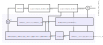
\includegraphics[width = 0.99\textwidth]{fig_C2_PBAdiagram.tex}
    \caption{Schematic diagram of the passivity-based adaptive controller (PBAC), where $\Sigma_{\textrm{softrobot}}$ denotes the dynamical system \eqref{eq:C2:dynamic_model} and $\Sigma_{\textrm{sensor}}$ a system of sensors suitable of measuring $\q$ and $\dq$. }
    \label{fig:C2:PBA_diagram}
  \end{figure}


\noindent where $\dq_r = \dq_d - \LambdaB \eB $ is called the reference velocity vector, $\LambdaB \in \R^{n \times n}$ a positive diagonal matrix, and $\vec{Y}(\q,\dq,\dq_r,\dq_r,\piB) \in \R^{m\times n}$ is called the regressor matrix. Following the work of Slotine and Li \cite{Slotine1988}, the control law and adaptation law are given by
%
\begin{align}
\tauB = &\, \tmat{M}\,\ddq_r + \tmat{C}\, \dq_r + \tvec{f}\!\grav +  \tvec{f}\!\elastic - \tvec{\delta} - \mat{K}_p \, \vec{e} - \mat{K}_d\, \vec{e}_r,  \label{eq:C2:tau} \\
\dot{\tvec{\pi}} =& - \mat{K}_{\vec{\pi}}\,\vec{Y}^\top\vec{e}_r,  \label{eq:C2:update}
\end{align}
%
where $\vec{e}_r := \dq - \dq_r = \dot{\vec{e}} + \LambdaB\,\vec{e}$, $\mat{K}_p, \mat{K}_d \in \mathbb{R}^{n\times n}$ are controller gains, and $\mat{K}_{\vec{\pi}} \in \R^{p\times p}$ is a positive definite matrix called the adaptation rate. Since $\tauB$ define the desired generalized forces acting on the system \eqref{eq:C2:dynamic_model}, the desired pressures are computed as $\uB = \mat{G}^{+} \tauB$ with $\mat{G}^{+}$ the generalized inverse of $\mat{G}$. A schematic diagram of the passivity-based controller is provided in Figure \ref{fig:C2:PBA_diagram}. It should be mentioned that the magnitude of adaptation rate does not affect the global stability of the system (if unmodelled dynamics are not excited); however, it sets the rate of adaptation, and accordingly the performance of the system.

\begin{rmk}[Persistence of excitation]
\label{rmk:C2:poe}
\editl It is important to note that the convergence of the tracking error $\eB \to 0$ does not imply convergence of the estimated parameter to their true values. According to \cite{Slotine1988,Slotine1989Jul,SlotineJ1987}, asymptotic convergence can be shown if the matrix $\vec{Y}(\q,\dq,\dq_r,\dq_r,\piB)$ is persistently excited and it is uniformly continuous. To elaborate, under the condition of persistent excitation, that is, for any instances $t_1,t_2$ with  $t_1\le t_2$  there exists a positive constant $\alpha$ such that $\int_{t_1}^{t_2} \mat{Y}^\top\,\mat{Y} \;dt \preceq \alpha\,\mat{I}$, it can be proven that the parameter estimates converge asymptotically to their true values. The authors in \cite{Slotine1988} state that the proof for convergence here applied to nonlinear robot dynamics is similar to those of linear dynamics \cite{Morgan1977} although the proof is fairly involved. \editr
\end{rmk}
%


\clearpage
\section{Numerical and experimental implementation}
\label{sec: chap2 section header}
%!TEX root = ../../thesis.tex
\noindent In this section, we will discuss the simulation results of the dynamic model \eqref{eq:C2:dynamic_model}, the passivity-based controller \eqref{eq:C2:tau}, and the adaptive law \eqref{eq:C2:update}. To illustrate effectiveness and performance of the approach, we segregate our analysis into several study-cases of various complexity. First, focusing on the physical one-link soft robot in Figure \ref{fig:C2:soft_robot} ($N = 1$), we investigate the unforced system's equilibria and their corresponding stability. In continuation, we compare the simulated trajectories of the dynamical model with experimental data for natural oscillations, forced pneumatic inputs, and external loading conditions; where we also highlight contribution of the hyper-elastic FEM-driven material model. Second, to illustrate the flexibility and computational efficiency of the numerical framework, we extend the one-link model to a multi-link model with $N = 6$ soft-bodied links.

The numerical solutions to the ordinary differential equations in \eqref{eq:C2:dynamic_model} together with \eqref{eq:C2:tau} and \eqref{eq:C2:update} are computed using the aforementioned MDE integration scheme which is developed in \matlab, and the underlying code can be found at Caasenbrood et al. (2020, \cite{Caasenbrood2021}). The software architecture is compactly written as Object-Oriented class labeled under \texttt{./src/Model.m} that enables a minimal programming interface to set-up various soft robotic simulation models easily. Additionally, all numerical examples that will be discussed in this section are made available under \texttt{./examples/paper} on the repository.
%
%\subsection*{Example 1: Natural dynamics -- One-link soft robot}
\begin{example}[Natural dynamics -- One-link soft robot]
\end{example}
\noindent The following physical parameters are chosen for the soft robot: the mass $m_0 = 17.3$ g, the relaxation length $l_0 = 64.4$ mm. The material parameters for hyper-elasticity and visco-elasticity models are chosen identical to Table \ref{tab:C2:elastic_parameters}. For the additional viscous material behavior, the Rayleigh damping matrix and the creep compliance matrix are chosen a follow:
%
\begin{align}
\mat{R} & = \begin{pmatrix} 0.01 & 0 & 0 \\ 0 &  1.05\pwr{-5} & 0 \\ 0 & 0 & 1.05\pwr{-5} \end{pmatrix}; \notag \\[0.45em]
\mat{K}_{\lambda} & = \begin{pmatrix} 502.3 & 0 & 0 \\ 0 &  1.53\pwr{-2} & 0 \\ 0 & 0 & 1.53\pwr{-2} \end{pmatrix}. \notag
\end{align}
%
\noindent We stress that the values for the Rayleigh damping and creep compliance shown above are identified empirically {through} open-loop measurements, similar to the creep coefficient provided in Table \ref{tab:C2:elastic_parameters}.
%The code for the one-link simulation model can be found under \texttt{./mdl\_1\_natural.m}.
%

First, we investigate the existence and the stability of the equilibria of the unforced system. If the system is at rest (i.e., $\dq = 0$, $\ddq = 0$), then by definition there are no conservative forces acting on the system. Thus, for any equilibrium point ${\q}_0$ it holds that $\nabla \mathcal{U}({\q}^\star) \equiv \vec{0}$. If $ \mathcal{U}({\q}^\star) \equiv E_0$ is a local minimum, then the equilibrium is deemed stable. Any small disturbance will result in a new energy-state $E_1$ and will consequently bring the system in motion. However, regarding $E_0$ is a local minimum, the system will remain in a neighborhood of ${\q}^\star$ and eventually converge towards its nearest low-state energy $E_0$. If $\mathcal{U}({\q}^\star) \equiv E_0$ is a local maximum, the equilibrium is deemed to be unstable, since there exist a configuration close to ${\q}^\star$ with a lower energy-state, \ie, $\mathcal{U}({\q}^\star + {\delta}\q) < E_1$.

By analysis of the gradient of the potential energy function $\nabla \mathcal{U}({\q})$, two unique equilibria can be found numerically. The potential function has a local maximum for $\q^\star_{\textrm{unstab}}=(-\tfrac{m_0 g}{L (\alpha_1 - \alpha_2)},\,0,\,0)^\top$ which is unstable. To some extent, it is analogous to the unstable upwards equilibrium position related to the single-DOF pendulum system. For the stable equilibria, the bisection method was used to find the zero-crossing of $\nabla \mathcal{U}({\q})$, where it was found that all stable solutions of the unforced system will tend to the following set:
%
\begin{equation*}
\Omega_{\textrm{stab}} = \left\{\q\in \mathcal{Q}\;:\;\varepsilon=\varepsilon^\star,\, \kappa(\q) = \frac{\alpha^\star}{\alpha_\phi(\q)} \right\} \notag
\end{equation*}
%
with $\varepsilon^\star = -0.0021$ and $\alpha^\star = 0.0174$, which topologically equivalent to a ring. This set corresponds to the hanging position of the soft robot. It should be worth mentioning that the stable set of equilibria stems from the force balance between the internal elastic potential forces and the external gravitational potential forces, and thus any stiffness will lead to a stable set with a similar topology. By changing the base orientation of the soft manipulator (i.e., by modifying $\Phi_0$), both equilibria vanish and all state trajectories will tend to a global stable equilibrium. For fully reversing the orientation, this trivially leads to the stable equilibrium $(\varepsilon,\,\kappa_x,\,\kappa_y) = (+\tfrac{m_0 g}{L (\alpha_1 - \alpha_2)},\, 0,\, 0)$. This phenomenon is referred to as local bifurcation, in which the change of parameter values alters the existence and stability of equilibria. This property might be interesting for soft robot manipulators with multiple soft-bodied links, as they are likely to be subjected to different gravitational loads.

To illustrate the unforced dynamics and the existence of stable equilibria, time-domain simulations of the dynamical model with nonzero initial conditions:
%
\begin{align*}
\q_0 & = \left(0,\,-15,\,15\; \right)^\top, \\[0.35em] \dq_0 & = \left(0,\,2500,\,0 \right)^\top
\end{align*}
%
Figure. \ref{fig:C2:natural_states} shows the state trajectories of the soft robot; whereas Figure \ref{fig:4}b is provided to better illustrate the underlying dynamics and the trajectory of the end-effector.
%
\begin{figure}[!t]
  \vspace{-5mm}
  \centering
  % This file was created by matlab2tikz.
%
\definecolor{mycolor1}{rgb}{0.00000,0.34510,0.65882}%
%
\begin{tikzpicture}

\begin{axis}[%
width=0.817\textwidth,
height=0.128\textwidth,
at={(0\textwidth,0.372\textwidth)},
scale only axis,
xmin=0,
xmax=0.8,
ymin=-0.002,
ymax=0.004,
ylabel style={font=\color{white!15!black}},
ylabel={$\varepsilon$ (-)},
axis background/.style={fill=white},
xmajorgrids,
ymajorgrids,
ylabel style={yshift=-3.5pt}
]
\addplot [color=mycolor1, line width=1.5pt, forget plot]
  table[row sep=crcr]{%
0	0\\
0.00100069999999997	0.00118280000000004\\
0.00200129999999998	0.00302690000000005\\
0.00300199999999995	0.00320659999999995\\
0.00400270000000003	0.00204000000000004\\
0.00500330000000004	0.00137810000000005\\
0.00600400000000001	0.00189989999999995\\
0.00700469999999997	0.00259039999999999\\
0.00800529999999999	0.00244929999999999\\
0.00900599999999996	0.00173400000000001\\
0.010007	0.00132149999999998\\
0.012008	0.0015965\\
0.013009	0.00129559999999995\\
0.014009	0.000752890000000006\\
0.01501	0.000412799999999991\\
0.016011	0.000345240000000024\\
0.017011	0.000263690000000039\\
0.018012	6.14200000004228e-06\\
0.0190129999999999	-0.000267059999999986\\
0.0200129999999999	-0.000355349999999977\\
0.022015	-0.000226130000000047\\
0.023015	-0.000218750000000045\\
0.024016	-0.000179099999999988\\
0.025017	-4.87319999999958e-05\\
0.026017	0.000119230000000026\\
0.027018	0.000247529999999996\\
0.029019	0.000416859999999963\\
0.031021	0.000616460000000041\\
0.032021	0.000675300000000045\\
0.0360240000000001	0.000792470000000045\\
0.038025	0.000790540000000006\\
0.041027	0.000757299999999961\\
0.043029	0.000692970000000015\\
0.046031	0.000568110000000011\\
0.0520350000000001	0.000254760000000021\\
0.056037	5.16750000000288e-05\\
0.059039	-7.46109999999467e-05\\
0.061041	-0.000132119999999958\\
0.063042	-0.00015993999999997\\
0.065043	-0.000150239999999968\\
0.067045	-0.000101770000000001\\
0.0690460000000001	-1.85299999999611e-05\\
0.072048	0.000146179999999996\\
0.0750500000000001	0.000311900000000032\\
0.077051	0.000399240000000023\\
0.079053	0.000458139999999996\\
0.081054	0.000486059999999955\\
0.083055	0.000485100000000016\\
0.085057	0.000460800000000039\\
0.088059	0.000394299999999959\\
0.0910610000000001	0.000299209999999994\\
0.094063	0.000176859999999945\\
0.10007	-8.26600000000122e-05\\
0.10207	-0.000138430000000023\\
0.10407	-0.000163899999999995\\
0.10607	-0.000156939999999994\\
0.10807	-0.000121860000000029\\
0.11107	-3.72770000000022e-05\\
0.11508	7.97289999999728e-05\\
0.11808	0.00013996000000005\\
0.12108	0.000169470000000005\\
0.12408	0.000173120000000027\\
0.12809	0.000150490000000003\\
0.13309	9.08080000000533e-05\\
0.1451	-7.99169999999849e-05\\
0.1501	-0.000113290000000044\\
0.1551	-0.000115599999999993\\
0.16111	-8.87210000000138e-05\\
0.17512	-1.33270000000074e-05\\
0.18212	-1.10450000000428e-05\\
0.19013	-3.9399000000051e-05\\
0.20714	-0.000110049999999973\\
0.21514	-0.000106530000000049\\
0.23716	-7.15239999999895e-05\\
0.25417	-9.7973000000029e-05\\
0.26918	-0.000108980000000036\\
0.36024	-0.000104609999999949\\
0.64943	-0.000108019999999986\\
0.80053	-0.000108019999999986\\
};
\end{axis}

\begin{axis}[%
width=0.817\textwidth,
height=0.128\textwidth,
at={(0\textwidth,0.186\textwidth)},
scale only axis,
xmin=0,
xmax=0.8,
ymin=-30,
ymax=30,
ylabel style={font=\color{white!15!black}},
ylabel={$\kappa_x$ (1/m)},
axis background/.style={fill=white},
xmajorgrids,
ymajorgrids,
ylabel style={yshift=-3.5pt}
]
\addplot [color=mycolor1, line width=1.5pt, forget plot]
  table[row sep=crcr]{%
0	-15\\
0.0160109999999989	21.093\\
0.0200129999999987	24.639\\
0.0220149999999997	24.921\\
0.0240159999999996	24.275\\
0.0280190000000005	20.825\\
0.0370249999999999	8.0954\\
0.0530350000000013	-14.326\\
0.0600400000000008	-19.584\\
0.0640430000000016	-20.462\\
0.0650429999999993	-20.405\\
0.0670450000000002	-19.956\\
0.0710470000000001	-17.783\\
0.0780519999999996	-10.912\\
0.0990660000000005	11.571\\
0.10407	13.835\\
0.10707	14.162\\
0.109069999999999	13.96\\
0.11308	12.693\\
0.120080000000002	8.6293\\
0.145099999999999	-7.5345\\
0.152100000000001	-9.6423\\
0.156099999999999	-10.114\\
0.158110000000001	-10.154\\
0.16011	-10.071\\
0.16311	-9.7278\\
0.168109999999999	-8.6433\\
0.176120000000001	-5.9078\\
0.203140000000001	4.2835\\
0.210139999999999	5.4359\\
0.21414	5.6507\\
0.215140000000002	5.6544\\
0.217140000000001	5.6043\\
0.22015	5.394\\
0.225149999999999	4.733\\
0.234159999999999	2.8837\\
0.257169999999999	-2.165\\
0.265180000000001	-3.1435\\
0.271180000000001	-3.478\\
0.274180000000001	-3.5186\\
0.275179999999999	-3.5142\\
0.277180000000001	-3.4797\\
0.281189999999999	-3.3144\\
0.287189999999999	-2.8582\\
0.296199999999999	-1.8413\\
0.321210000000001	1.1479\\
0.329219999999999	1.6489\\
0.334219999999998	1.7913\\
0.337219999999999	1.8136\\
0.339230000000001	1.8034\\
0.342230000000001	1.7526\\
0.34723	1.5834\\
0.355239999999998	1.144\\
0.387260000000001	-0.82525\\
0.394259999999999	-0.9984\\
0.39827	-1.0371\\
0.400269999999999	-1.0405\\
0.402270000000001	-1.0338\\
0.405270000000002	-1.0058\\
0.410270000000001	-0.91602\\
0.418279999999999	-0.684049999999999\\
0.452300000000001	0.438210000000002\\
0.458310000000001	0.51538\\
0.462309999999999	0.53706\\
0.464310000000001	0.53923\\
0.467310000000001	0.53219\\
0.471309999999999	0.504999999999999\\
0.477319999999999	0.431660000000001\\
0.48732	0.250540000000001\\
0.510339999999999	-0.179390000000001\\
0.518350000000002	-0.263059999999999\\
0.524349999999998	-0.29299\\
0.527349999999998	-0.2974\\
0.530349999999999	-0.295110000000001\\
0.53436	-0.28246\\
0.54036	-0.245730000000002\\
0.54937	-0.161860000000001\\
0.575379999999999	0.0987620000000007\\
0.583390000000001	0.141269999999999\\
0.589390000000002	0.155419999999999\\
0.593399999999999	0.156510000000001\\
0.5974	0.151420000000002\\
0.602399999999999	0.137350000000001\\
0.610410000000002	0.101030000000002\\
0.643429999999999	-0.0701439999999991\\
0.65043	-0.0844270000000016\\
0.655439999999999	-0.0876699999999992\\
0.660440000000001	-0.0854430000000015\\
0.666440000000001	-0.0764409999999991\\
0.67445	-0.0562310000000004\\
0.707470000000001	0.0381\\
0.715479999999999	0.0465310000000017\\
0.72148	0.0475339999999989\\
0.728490000000001	0.0435039999999987\\
0.737490000000001	0.0319460000000014\\
0.773520000000001	-0.0228089999999987\\
0.78152	-0.0262239999999991\\
0.789529999999999	-0.0253240000000012\\
0.799530000000001	-0.0192890000000006\\
0.800529999999998	-0.0184619999999995\\
};
\end{axis}

\begin{axis}[%
width=0.817\textwidth,
height=0.128\textwidth,
at={(0\textwidth,0\textwidth)},
scale only axis,
xmin=0,
xmax=0.8,
xlabel style={font=\color{white!15!black}},
xlabel={time (s)},
ymin=-30,
ymax=30,
ylabel style={font=\color{white!15!black}},
ylabel={$\kappa_x$ (1/m)},
axis background/.style={fill=white},
xmajorgrids,
ymajorgrids,
ylabel style={yshift=-3.5pt}
]
\addplot [color=mycolor1, line width=1.5pt, forget plot]
  table[row sep=crcr]{%
0	15\\
0.00100070000000052	14.95\\
0.00400269999999914	14.297\\
0.0100069999999999	11.814\\
0.0160110000000007	7.6573\\
0.0370249999999999	-9.5688\\
0.0420280000000002	-11.059\\
0.0450300000000006	-11.31\\
0.0460309999999993	-11.287\\
0.0480319999999992	-11.09\\
0.0520350000000001	-10.147\\
0.0580390000000008	-7.5546\\
0.0680449999999997	-1.1197\\
0.0800529999999995	6.0245\\
0.0870580000000007	8.3962\\
0.0930619999999998	9.3567\\
0.0950629999999997	9.4097\\
0.0970650000000006	9.3007\\
0.100070000000001	8.8078\\
0.10507	7.1137\\
0.11408	2.2559\\
0.12809	-5.0254\\
0.136089999999999	-7.5037\\
0.14109	-8.152\\
0.1431	-8.2116\\
0.1441	-8.1999\\
0.146100000000001	-8.0963\\
0.1501	-7.5893\\
0.1561	-6.1972\\
0.167109999999999	-2.4697\\
0.183120000000001	2.8362\\
0.191129999999999	4.4719\\
0.19713	5.1057\\
0.201129999999999	5.2204\\
0.203139999999999	5.1825\\
0.20614	5.008\\
0.21114	4.4251\\
0.219150000000001	2.9017\\
0.24516	-2.5238\\
0.25217	-3.2225\\
0.25717	-3.4262\\
0.259169999999999	-3.4404\\
0.26117	-3.4181\\
0.26418	-3.3202\\
0.26918	-3.0039\\
0.27718	-2.1924\\
0.30921	1.4497\\
0.31621	1.7737\\
0.320209999999999	1.8472\\
0.32221	1.8539\\
0.32422	1.8412\\
0.327220000000001	1.7872\\
0.33222	1.6127\\
0.34023	1.1607\\
0.37125	-0.826919999999999\\
0.37825	-1.0173\\
0.38326	-1.0668\\
0.384259999999999	-1.0684\\
0.387259999999999	-1.0571\\
0.391260000000001	-1.0076\\
0.397259999999999	-0.869759999999999\\
0.406269999999999	-0.56235\\
0.431290000000001	0.34328\\
0.43929	0.500870000000001\\
0.4453	0.555770000000001\\
0.4483	0.56293\\
0.4513	0.557230000000001\\
0.455299999999999	0.53106\\
0.461309999999999	0.457409999999999\\
0.47031	0.29191\\
0.495329999999999	-0.195040000000001\\
0.50334	-0.27852\\
0.50934	-0.30663\\
0.51234	-0.30972\\
0.51534	-0.30593\\
0.519349999999999	-0.290929999999999\\
0.52535	-0.25001\\
0.535360000000001	-0.14809\\
0.55837	0.0959800000000008\\
0.566380000000001	0.144310000000001\\
0.572380000000001	0.16215\\
0.57638	0.165240000000001\\
0.58039	0.1617\\
0.58539	0.14888\\
0.59239	0.11825\\
0.6044	0.0460480000000008\\
0.62041	-0.0462399999999992\\
0.62942	-0.0787340000000007\\
0.63542	-0.0896410000000003\\
0.64043	-0.092041\\
0.645429999999999	-0.0887689999999992\\
0.652430000000001	-0.0760450000000006\\
0.661440000000001	-0.0497449999999997\\
0.68746	0.0322759999999995\\
0.695460000000001	0.0455330000000007\\
0.70247	0.0501120000000004\\
0.70847	0.049004\\
0.715479999999999	0.0426590000000004\\
0.725479999999999	0.0269060000000003\\
0.7525	-0.0191949999999999\\
0.761509999999999	-0.0263190000000009\\
0.76951	-0.0276610000000002\\
0.777520000000001	-0.0247609999999998\\
0.78853	-0.0157760000000007\\
0.80053	-0.00321839999999973\\
};
\end{axis}
\end{tikzpicture}%
  \vspace{-3mm}
  \caption{Three-dimensional volumetric evolution of the one-link soft robot model with initial conditions $\q_0 = (0 , -15, 15)^\top$ and $\dq_0 = (0, 2500, 0)^\top$. Notice that the soft robot oscillates about the set of stable equilibria $\Omega_{\textrm{stab}}$. }
  \label{fig:C2:natural_states}
\end{figure}
%
%
\begin{figure}[!t]
  %\vspace{-3mm}
  \centering
  % This file was created by matlab2tikz.
%
%The latest updates can be retrieved from
%  http://www.mathworks.com/matlabcentral/fileexchange/22022-matlab2tikz-matlab2tikz
%where you can also make suggestions and rate matlab2tikz.
%
\begin{tikzpicture}

\begin{axis}[%
width=0.216\textwidth,
height=0.199\textwidth,
at={(0\textwidth,0.253\textwidth)},
scale only axis,
axis on top,
xmin=0.5,
xmax=522.5,
tick align=outside,
y dir=reverse,
ymin=0.5,
ymax=458.5,
axis line style={draw=none},
ticks=none,
ylabel style={yshift=-7.5pt}
]
\addplot [forget plot] graphics [xmin=0.5, xmax=522.5, ymin=0.5, ymax=458.5] {fig_C2_natural_3D-1.png};
\end{axis}

\begin{axis}[%
width=0.216\textwidth,
height=0.199\textwidth,
at={(0.245\textwidth,0.253\textwidth)},
scale only axis,
axis on top,
xmin=0.5,
xmax=522.5,
tick align=outside,
y dir=reverse,
ymin=0.5,
ymax=458.5,
axis line style={draw=none},
ticks=none,
ylabel style={yshift=-7.5pt}
]
\addplot [forget plot] graphics [xmin=0.5, xmax=522.5, ymin=0.5, ymax=458.5] {fig_C2_natural_3D-2.png};
\end{axis}

\begin{axis}[%
width=0.216\textwidth,
height=0.199\textwidth,
at={(0.49\textwidth,0.253\textwidth)},
scale only axis,
axis on top,
xmin=0.5,
xmax=522.5,
tick align=outside,
y dir=reverse,
ymin=0.5,
ymax=458.5,
axis line style={draw=none},
ticks=none,
ylabel style={yshift=-7.5pt}
]
\addplot [forget plot] graphics [xmin=0.5, xmax=522.5, ymin=0.5, ymax=458.5] {fig_C2_natural_3D-3.png};
\end{axis}

\begin{axis}[%
width=0.216\textwidth,
height=0.199\textwidth,
at={(0.734\textwidth,0.253\textwidth)},
scale only axis,
axis on top,
xmin=0.5,
xmax=522.5,
tick align=outside,
y dir=reverse,
ymin=0.5,
ymax=458.5,
axis line style={draw=none},
ticks=none,
ylabel style={yshift=-7.5pt}
]
\addplot [forget plot] graphics [xmin=0.5, xmax=522.5, ymin=0.5, ymax=458.5] {fig_C2_natural_3D-4.png};
\end{axis}

\begin{axis}[%
width=0.216\textwidth,
height=0.199\textwidth,
at={(0\textwidth,0\textwidth)},
scale only axis,
axis on top,
xmin=0.5,
xmax=522.5,
tick align=outside,
y dir=reverse,
ymin=0.5,
ymax=458.5,
axis line style={draw=none},
ticks=none,
ylabel style={yshift=-7.5pt}
]
\addplot [forget plot] graphics [xmin=0.5, xmax=522.5, ymin=0.5, ymax=458.5] {fig_C2_natural_3D-5.png};
\end{axis}

\begin{axis}[%
width=0.216\textwidth,
height=0.199\textwidth,
at={(0.245\textwidth,0\textwidth)},
scale only axis,
axis on top,
xmin=0.5,
xmax=522.5,
tick align=outside,
y dir=reverse,
ymin=0.5,
ymax=458.5,
axis line style={draw=none},
ticks=none,
ylabel style={yshift=-7.5pt}
]
\addplot [forget plot] graphics [xmin=0.5, xmax=522.5, ymin=0.5, ymax=458.5] {fig_C2_natural_3D-6.png};
\end{axis}

\begin{axis}[%
width=0.216\textwidth,
height=0.199\textwidth,
at={(0.49\textwidth,0\textwidth)},
scale only axis,
axis on top,
xmin=0.5,
xmax=522.5,
tick align=outside,
y dir=reverse,
ymin=0.5,
ymax=458.5,
axis line style={draw=none},
ticks=none,
ylabel style={yshift=-7.5pt}
]
\addplot [forget plot] graphics [xmin=0.5, xmax=522.5, ymin=0.5, ymax=458.5] {fig_C2_natural_3D-7.png};
\end{axis}

\begin{axis}[%
width=0.216\textwidth,
height=0.199\textwidth,
at={(0.734\textwidth,0\textwidth)},
scale only axis,
axis on top,
xmin=0.5,
xmax=522.5,
tick align=outside,
y dir=reverse,
ymin=0.5,
ymax=458.5,
axis line style={draw=none},
ticks=none,
ylabel style={yshift=-7.5pt}
]
\addplot [forget plot] graphics [xmin=0.5, xmax=522.5, ymin=0.5, ymax=458.5] {fig_C2_natural_3D-8.png};
\end{axis}

\begin{axis}[%
width=0.969\textwidth,
height=0.51\textwidth,
at={(-0.01\textwidth,-0.029\textwidth)},
scale only axis,
xmin=0,
xmax=1,
ymin=0,
ymax=1,
axis line style={draw=none},
ticks=none,
axis x line*=bottom,
axis y line*=left,
ylabel style={yshift=-7.5pt}
]
\end{axis}
\end{tikzpicture}%
  \vspace{-3mm}
  \caption{State trajectories of one-link soft robot model with initial conditions $\q_0 = (0 , -15, 15)^\top$ and $\dq_0 = (0, 2500, 0)^\top$. The figure shows the elongation strain $\varepsilon$ and the curvatures $\kappa_x$, $\kappa_y$ in the $xz$-plane and $yz$-plane, respectively.}
  \label{fig:C2:natural_3D}
\end{figure}
%
Besides the existence of stable solutions, the numerical simulations perfectly illustrate the coupled dynamics between the elongation and bending of the soft robot. Due to the difference in mechanical stiffness for elongation and bending, we observe high-frequency and low-frequency oscillation for the elongation strain $\varepsilon(t)$, and we observe low-frequent oscillations for the curvatures $\kappa_x(t)$ and $\kappa_y(t)$. Interestingly, the low-frequency oscillations are passed from the curvature dynamics to elongation dynamics; conversely, the dynamics of the elongation barely affect the curvatures. After sufficient time passes, the trajectories indeed tend to the set of stable equilibria $\Omega$.

\subsection{Experimental platform}
\noindent Before validating the one-link dynamic model, we detail the experimental setup and control platform of the soft robotic system. We would like to briefly emphasize that sensing is a challenging topic soft robotics, due large continuous deformations and the presence of sensors that might affect the system's dynamics. As such, a combination of integrated sensors were used to recover an estimate of the states $\q \in \mathcal{Q}$. First of all, we employed a 9-DOF inertial measurement unit (Bosch, BNO055) measures the angular displacement of the soft robot's end-effector (i.e., $\sigma = L$). Through on-board sensor fusion, the bending angle of the soft robot can be recovered, i.e., $\beta = \kappa l$. Since the bending angle alone is not sufficient to decouple the curvature and elongation, additional sensing is required. Consequently, we used a vision sensor (\texttt{CreateLab}, \texttt{PixyCam2}) with an embedded processor (\texttt{NXP LPC44330}, 200 MHz) for optical tracking. A spherical optical marker is attached to the end-effector of the soft robot. Through trigonometry and the measured bending angle $\beta$, an estimate of the position vector $\gammaB(L,\q)$ can be recovered. Given the analytic expressions for the orientation and position in \eqref{eq:C2:phi_exact} and \eqref{eq:C2:pos_vector}, an inverse Jacobian kinematic solver is employed to recover an estimate of the state vector $\tvec{q}_d$.
During each experimental trail, it was made sure the soft robotic body does not occlude the optical marker.

As for the pneumatic actuation, an array of proportional-pressure regulators (Festo, VEAB-B-D16) was used with an active pressure range of $-0.1 \;\text{MPa}\, < \uB(t) \le 0.1 \; \textrm{MPa}$, which simultaneously allow for pressure measurements. These measurements are fed into the (quasi-static) model to also recover a quasi-static estimate of the states $\hat{q}_s$. Then, the dynamic estimates $\tvec{q}_{\textrm{dyn}}$ and the quasi-static pressure-based estimates $\tvec{q}_{\textrm{qs}}$ are fused using a complementary filter. The control and data acquisition are done using a \texttt{Raspberry Pi 4} (\texttt{2GB}). The full experimental setup can be seen in Figure \ref{fig:5}.

\begin{example}[Model validation -- unforced, forced, and external loads]
\noindent To validate the dynamic model, the solutions of the model are compared with measurements of the physical system in unforced,  forced, and tip-load conditions. As such, the model validation is separated into three parts: \textit{i)} unforced, \textit{ii)} forced conditions, and \textit{i)} external tip-loads applied on the end-effector. We start with the unforced scenario, \ie, no input is considered $u_i(t) \equiv 0$. For the unforced analysis, two experimental trails are performed for the unforced validation. First, the soft robot is deformed slightly and then released from rest, which corresponds to the initial conditions $\q_0 = \left(\;0.015,\,4.75,\,0\; \right)^\top$ and $\dq_0 = 0_3$. Since the mechanical deformations are relatively small here, the presence of hyper-elastic and visco-elastic material behavior are less dominant. Secondly, the soft robot is moderately deformed such that the initial configuration (or shortly after) lies within the hyper-elastic and visco-elastic regime. In this scenario, the nonlinear and time-dependent material effects may not be neglected. These initial conditions correspond to $\q_0 = \left(\;0.046,\,11.25,\,0\; \right)^\top$ and $\dot{{q}}_0 = 0_3$. It is worth mentioning that the creep strains $\lambda$ are difficult to distinguish from the true strain, and thus the initial conditions for $\lambda(t_0)$ are determined empirically. The validation results for both unforced scenario are shown in Figure \ref{fig:6}a. The associated code for the unforced validation simulations can be found under \texttt{./valid\_one\_link\_open.m}.
\end{example}

%
\begin{figure}[!t]
\centering
%\includegraphics[width = 0.95\textwidth]{CaasenbroodFig6.eps}
\caption{\textbf{(a)} Validation results of the
dynamic model in unforced conditions, where the dashed lines represent the experimental measurements and the solid lines are the simulated trajectories. \textbf{(b)} Validation results of the dynamic model in forced conditions, where the dashed lines represent the experimental data from the inertial sensor and the solid lines simulated. In addition, the figure also illustrates the model for Hookean elasticity and applied pressure inputs $u(t)$ to the dynamical system. It is evident from these comparison results that FEM-driven elasticity models can significantly improve accuracy. \textbf{(c)} Experimental validation of the one-link soft robot subjected to various end-effector payloads of different mass $m_\delta = \{0.05,\,0.1,\,0.15\}$ kg. \textbf{(d)} The quasi-static deformation produced by the hyper-elastic model under various end-effector loads. In both figures, the solid lines represent the dynamic model and the dashed lines are the experimental measurements. \label{fig:6}}
\end{figure}
%
As can be seen, the state trajectories of the end-effector closely match the ground truth trajectories, even for significant nonlinear deformation. For the first validation run (inside linear elastic regime), the RMS error and the maximum error are $\pm0.19$ and $\pm 0.50$ degrees, respectively. For the second case (outside the linear elastic regime), the RMS error and the maximum error is $\pm0.78$ and $\pm 2.33$ degrees, respectively.

Second, we consider a forced scenario in which a regulated pressure input is applied to the pneumatic bellows. Since the pneumatic mapping $H$ in \eqref{eq:mapping_H} plays an important role here, the actuator coefficients are recomputed to match the experimental data better. To be more specific, by considering a pre-defined set of excitation signals $u(t)$ of various amplitudes and frequencies, a least-squares optimization routine is employed that minimizes the difference between the measured states $\hat{q}$ with the simulated states ${q}$ by tuning the coefficients $\alpha_\varepsilon$ and $\alpha_\kappa$. This leads to the following values: $\alpha_\varepsilon = 2.34\cdot 10^{-7}$ and $\alpha_\kappa =  1.61\cdot 10^{-8}$. As for the excitation signal, we have chosen the following input:
%
\begin{equation}
u_i(t) = P_0 + P_A \left[\frac{1}{2} + \frac{1}{2}\sin(t + \phi_i) \right]\cdot \max(0.05t,1),
\end{equation}
%
with a static offset $P_0 = 10$ kPa, an amplitude $P_A = 25$ kPa, and a phase offset $\phi_i = (i-1)\frac{2\pi}{m}$ rad. To highlight the significance of the proposed hyper-elastic modeling approach, we also compare the results using an optimized Hookean material material model with $k_e = 50.6$ N/m and $k_b = 5.8\cdot 10^{-4}$ Nm/rad. The initial conditions are set to zero. The validations results for both the FEM-driven hyper-elasticity model and linear model in the forced setting are shown in Figure \ref{fig:6}b. The figure also shows the measured outputs from the pneumatic VEAB regulators $u_i(t)$, which are directly fed into both linear and hyper-elastic models. The associated code for the forced validation can be found under \texttt{./valid\_one\_link\_closed.m}.

Given these results, two key observations can be made. First, both the linear Hookean and hyper-elastic models provide reasonable accuracy for small deformations $0 \le \kappa(t) \le 3$ with a RMS error of $\pm0.13$ and $\pm0.16$ in curvature, respectively. However, as deformations exceed the linear regime, the hyper-elastic model significantly outperforms the Hookean model. Focusing on the hyper-elastic model, both the asymmetric stiffness in radial direction and the strain-hardening are captured well, where the the linear models is not sufficiently rich to capture the material effects. The overall RMS errors for the linear and hyper-elastic model are $\pm1.79$ and $\pm0.21$ in curvature, respectively. Regarding the end-effector accuracy, the overall RMS errors for the linear and hyper-elastic model are $\pm2.58$ and $\pm0.65$ mm, respectively; which translates to an arc-length normalized error of $\pm4.09\%$ and $\pm1.03\%$. These validations results show that introducing nonlinear elastic effects driven by FEM-data can further improve the accuracy for a larger region of the soft robot's workspace.

For the last validation case, we subject the soft robot to an external payload of mass $\delta_m$ located at the end-effector. To model the disturbance, we use the expression for the external payload disturbance model $\delta_m$ in \eqref{eq:delta_payload}. The goal here is \textit{i)} to demonstrate the accuracy of the proposed payload model and quasi-static behavior of the dynamic model, and \textit{ii)} to highlight the limitations of the PCC assumptions under certain conditions. In this analysis, we consider three different payloads $m_\delta = \{0.05,\,0.1,\,0.15\}$ kg.
The experimental results of the payloads deformations are shown in Figure \ref{fig:6}c, and the resulting quasi-static deformations of the dynamic model are shown in Figure \ref{fig:6}d. The associated code for the external payload simulations can be found under \texttt{./valid\_one\_link\_tipload.m}.

As can be seen, the quasi-static behavior of the dynamic model matches the experimental results relatively well for smaller payloads. For the mass $m_\delta = 0.05$ kg, the Euclidean error between the model and the measurement are $\pm1.31$ mm. Increasing the payload to $m_\delta = 0.1$ kg leads to an error of $\pm2.15$ mm. We can also clearly observe that the estimate of the backbone curve subject to the PCC condition is beginning to deviate from the ground truth yet the overall shape still matches the experimental data. Lastly, by further increase the payload $m_\delta = 0.15$ kg, we clearly observe the limitations of the PCC condition under external loads -- with an end-effector error of $3.98$ mm. Also, there is a clear discrepancy in the backbone curve of the model and the ground truth, which might imply the PCC condition is no longer valid here as the payload could induce non-constant curvatures along the backbone. A possible solution might be to introduce a different shape parametrization, similar to the works \cite{Chirikjian1994,Boyer2021,Renda2020,DellaSantina2020}.

\begin{example}[Model benchmark -- Multi-link soft manipulator case]
\noindent In this section, we benchmark the proposed numerical integration scheme for a dynamic model of a six-link soft robot manipulator ($N = 6$). Here, we want to highlight that sufficient numerical speed can be obtained while preserving sufficient numerical precision. This is an important criteria for model-based control, as slow numerical models lack transferability from theory to application. As mentioned earlier, the numerical integration of the Lagrangian entities is the computational bottleneck. Although the MDE solver does aid with numerical performance; ultimately, using a balanced spatial and temporal discretization impacts real-time performance the most. Trivially, using larger stepsize -- both in space and time -- lead to a decrease in numerical precision; and in some cases numerical instability. In this benchmark, we investigate these effects by varying two solver parameters: the spatial stepsize of the explicit MDE solver denoted by $\Delta \sigma$ and the temporal stepsize of the implicit trapezoidal solver denoted by $\Delta t$. For convenience, we represent these stepsizes as standardized parameters: the number of finite elements $N_s = L/\Delta \sigma$ and the implicit solver frequency $f_s = \Delta t\inv$. For the benchmark, we choose a total length of $L = 0.15$ m and simulation time of $T = 10$ s.
\end{example}

%
The extension to the multi-link soft robot ($N = 6$) can be described by a following generalized coordinates with the following structure:
%
\begin{equation}
\q = \left(\,\varepsilon_1,\,\kappa_{x,1},\kappa_{y,1},...,\varepsilon_6,\,\kappa_{x,6},\kappa_{y,6} \, \right)^\top \in \mathcal{Q}
\end{equation}
%
To ensure the soft manipulator is self-supporting, we introduce slight variations to the hyper-elastic stiffness, link lengths, and the inertial properties of the dynamical system. Considering homogeneity, all links are chosen identical in length and mass: intrinsic link length $L_i = 0.025$ m and mass $m_i = 0.05$ kg. Next, the bending stiffness is slightly altered where we choose $\alpha_3 = 0.425$ Nm/rad and $\alpha_4 = 0.4$ Nm/rad. Please note that the material domain is now given by $\Xs = [0,\sum^N_{i=1} L_i]$. To introduce some interesting dynamics for the benchmark, we purely excite the first link of the serial-chain soft robot manipulator with a harmonic input:
%
\begin{align}
u_i(t) = \begin{cases}
P_a \cos(t) & \text{for} \; i = 1, \\
0 & \text{otherwise},
\label{eq:harm_freq}
\end{cases}
\end{align}
%
where $P_a = 125$ kPa is the pressure amplitude. As for the pneumatic mapping that converts pressure to joint torques, we choose $\tau = \left(H \otimes I_6 \right)u $ as the corresponding pneumatic map for the six-link soft manipulator. In total 36 benchmark simulations with different solver settings were performed and tested for their precision relative to a high-precision model ($f_s = 500$ Hz and $N_s = 500$). The state trajectories of the high-precision model are shown in Figure \ref{fig:7}a, whereas Figure \ref{fig:7}b is provided to highlight the underlying dynamics and the trajectory of the end-effector. The results for all benchmark simulations are shown in Table \ref{tab:benchmark_table}. The associated code for the six-link simulations can be found under \texttt{./benchmark\_six\_link.m} on the repository.

%
\begin{figure}[!t]
\centering
%\includegraphics[width =0.475\textwidth]{CaasenbroodFig7.eps}
\caption{\textbf{(a)} State trajectories of six-link soft robot model under dynamic excitation. The figure shows the extensible elongation strains and the total curvature $\kappa = \sqrt{\kappa_x^2 + \kappa_x^2}$ (as the dynamics are planar). \textbf{(b)} The three-dimensional representation of the end-effector trajectory of the six-link soft robot. Notice that the dynamics of the six-link robot converge to a periodic solution. \label{fig:7}}
\end{figure}

Let us first discuss the dynamics of the six-link soft manipulator subjected to a harmonic input. Given this relatively straightforward harmonic excitation, some interesting (stable) nonlinear dynamics appear. Although we excite the system using one harmonic, the dynamics of the soft robot show a rich collection of harmonic oscillations -- highlighting its nonlinear nature. Furthermore, after a short transient time (i.e., $t < 5$), the solutions of the multi-link soft robotic system tend to a so-called \emph{periodic solution}. Here, a solution is called periodic if there exists a period time $T_c >  0$ such that $\q(t) = \q(t + T_c)$ for all time $t$. Similar observations of the existence of periodic solutions (and control of such oscillations) were reported by Della Santina et al. \cite{Santina2021} for articulated soft robots. Given the harmonic excitation in \eqref{eq:harm_freq}, the period time here is $T_c = 1$.

Now, we can exploit these periodic solutions for benchmarking the numerical solver in which we compare the solution of a high-resolution model (i.e., ground truth) to the benchmark solution. Let us define the benchmark error as the Euclidean distance between the two periodic solutions:
%
\begin{align}
e & = \int^{T_c}_0 || \,^0\hat{p}(q(t),L) - \,^0p(q(t),L) || \; dt, \notag \\ & \approx \frac{1}{W}\sum_{i = 1}^{W} || \,^0\hat{p}(q(t_i),L) - \,^0p(q(t_i),L)) ||,
\end{align}
%
where $W$ is the number of time samples of the benchmark model inside the time interval of the periodic solution, and $^0\hat{p}(\cdot,L)$ and $^0p(\cdot,L)$ the tip position of the benchmark and the ground truth, respectively. The index $W$ naturally depends on the sampling frequency of the implicit solver. Table 2 shows the normalized errors (i.e., the tracking error $e$ normalized with the manipulator length $L$) together with the effective computation times of the numerical solver.
\clearpage


\begin{sidewaystable}[!t]
% \begin{landscape}
% \begin{table}
\caption{Benchmark results of the six-link soft robot manipulator for various temporal and spatial discretizations ($T =10$ s). The tables shows the mean tracking error of the end-effector relative to a ground truth ($f_s = 500$ Hz and $N_s = 500$ elements). The RMS errors are normalized with the total length $L = 0.15$ (i.e., the errors are presented in $\%$). The CPU times are also given; where the light-gray entries achieve real-time computation (consistently).  \label{tab:benchmark_table}}
\centering

\begin{tabular}{l|lllllll}
%\toprule
$N = 6$ s  & $N_s = 24$ & $N_s =36$ &  $N_s =60$ &  $N_s = 90$ & $N_s = 120$ & $N_s =180$ \\[0.15em]
%\midrule
$f_s = 25$ Hz &  \textcolor{deepcolor}{\small{19.0 / 1.77s }} &  \textcolor{deepcolor}{\small{9.37 / 2.54s }} & \textcolor{deepcolor}{\small{5.36 / 4.06s }} &  \textcolor{deepcolor}{\small{4.63 / 5.98s }} &  \textcolor{deepcolor}{\small{4.62 / 7.93s}} & \small{4.43 / 11.75s } \\ [0.5em]
$f_s = 50$ Hz &  \textcolor{deepcolor}{\small{17.5 / 3.50s }} &  \textcolor{deepcolor}{\small{7.04 / 5.04s }} &  \textcolor{deepcolor}{\small{4.33 / 6.73s}} & \small{3.69 / 11.60s } & \small{3.60 / 15.3s} & \small{3.69 / 22.71s } \\ [0.5em]
$f_s = 75$ Hz &  \textcolor{deepcolor}{\small{13.77 / 5.31s}} &  \textcolor{deepcolor}{\small{5.80 / 7.56s}} & \small{4.51 / 12.41s} & \small{4.22 / 17.49s} & \small{3.68 / 22.35s} & \small{3.72 / 33.33s} \\ [0.5em]
$f_s = 100$ Hz &  \textcolor{deepcolor}{\small{14.73 / 6.48s}} &  \textcolor{deepcolor}{\small{6.12 / 9.10s}} & \small{4.42 / 14.54s} & \small{3.71 / 21.46s} & \small{3.53 / 28.35s} & \small{2.89 / 42.03s} \\ [0.5em]
$f_s = 150$ Hz &  \textcolor{deepcolor}{\small{15.22 / 7.26s}} &  \textcolor{deepcolor}{\small{5.73 / 9.78s}} & \small{4.32 / 15.58s} & \small{3.46 / 23.07s} & \small{3.16 / 30.38s } & \small{2.67 / 45.06s } \\ [0.5em]
$f_s = 250$ Hz & {\small{14.61 / 11.98s}} & \small{5.32 / 16.71s} & \small{4.14 / 27.11s} & \small{3.35 / 40.19s} & \small{2.86 / 53.06s } & \small{2.21 / 78.61s } \\[0.5em]
%\bottomrule
\end{tabular}
\end{sidewaystable}
%\begin{landscape}

\clearpage
The benchmark table above gives some useful insight into which settings benefit numerical precision and speed the most. First, regarding the coarser models $N = 24$ (i.e., 4 elements per link), we observe large numerical errors of $>\!10\%$ independent of solver frequency. Although one could argue these settings grantee real-time performance (2s of simulation time for 1s computation at $N_s = 24$, $f_s = 75$ Hz) and might suffice for model-based control in slow settings (i.e., set-point stabilization), they are most likely unsuited for dynamic tracking objectives. Moving towards $N_s = 60$ (i.e., 10 elements per link), we observe a significant improvement in numerical precision $\pm4\%$ and while still retaining real-time performance (1.6s of simulation time for 1s computation time at $f_s = 50$ Hz). As such, these settings show that both numerical precision and real-time computation can be achieved for more complicated multi-links soft robots. However, regarding the high-accuracy models $N_s > 100$, we see only a slight increase in numerical precision $\pm3\%$ yet lose real-time capabilities. Consequently, these models might be suited for offline simulations, but lack transferability to online model-based control. However, a possible solution here might be to convert the \texttt{MATLAB} model into a \texttt{C} or \texttt{C++} equivalent model to further increase numerical speed \cite{Grazioso2019,Sadati2020}.

\begin{example}[Closed-loop control -- Passivity-based controller under material certainty and mass disturbance]
\noindent In the last numerical analysis, we demonstrate the results of the proposed passivity-based adaptive scheme. Due to its compactness and computational speed, we again consider the model of the one-link soft robot as seen in previous simulations. To illustrate the robustness of the controller, we purposely introduce some uncertainties. First, we introduce uncertainties in the hyper-elastic material parameters that deviate moderately from their true values in Table 1. Second, we introduce a payload to the end-effector of mass $m_\delta = 0.1$ kg. We again model this external disturbance using the relation in \eqref{eq:delta_payload}. Following the linear parametrizability of the uncertainties, the parameter estimation vector yields:
\end{example}
%
\begin{equation}
\tvec{\pi}(t) = \left( \tilde{\alpha}_1,\,\tilde{\alpha}_2,\,\tilde{\alpha}_4,\, \tilde{\alpha}_5,\, \tilde{m}_\delta\right)^\top,
\end{equation}
%
with initial conditions $\tvec{\pi}(t_0) = \tvec{\pi}_0 = \left(0.75 {\alpha}_1,\,0.75{\alpha}_2,\,0.45{\alpha}_4,\, 0.45{\alpha}_5,\, 0.65{m}_\delta\right)^\top$. Furthermore, the feedback gains and the adaptation rate are chosen as diagonal matrices as follows $K_p = \text{diag}(5,5\text{e-}5,5\text{e-}5)
$, $K_d = \text{diag}(1,1\text{e-}5,1\text{e-}5)$, $\Lambda = I_3$, and $K_\Pi =  \text{diag}(5\text{e}3,5\text{e}3,2\text{e-}6,2\text{e-}6,2\text{e-}2)$. These values were found to yield the best performance while avoiding noticeable oscillations in the closed-loop dynamics. Lastly, the following reference trajectory is considered:
%
\begin{equation}
\q_d(t) = \left(0.01 + 0.01\,\sin(t),\, 30 \,\sin(t),\, 30 \,\cos(t)\right)^\top,
\end{equation}
%
Since the reference trajectory above satisfies persistence of
excitation (see Remark 2), it should grantee the all convergence of the hyper-elastic material estimation and the unknown mass contribution. Figure \ref{fig:8}a shows the state trajectories of the soft robot, Figure \ref{fig:8}b is provided to better illustrate the underlying dynamics of the controller, and Figure \ref{fig:9} shows the evolution of the nonlinear stiffnesses estimates, $\hat{k}_e(q,\hat{\Pi})$ and $\hat{k_b}(q,\hat{\Pi})$, respectively; and the payload estimate $\hat{m}_\delta(\hat{\Pi})$.

%
\begin{figure}[!t]
  \vspace{-5mm}
  \centering
  % This file was created by matlab2tikz.
%
\definecolor{mycolor1}{rgb}{0.80392,0.80392,0.80392}%
\definecolor{mycolor2}{rgb}{0.00000,0.34510,0.65882}%
%
\begin{tikzpicture}

\begin{axis}[%
width=0.807\textwidth,
height=0.129\textwidth,
at={(0\textwidth,0.371\textwidth)},
scale only axis,
xmin=0,
xmax=60,
ymin=-0.005,
ymax=0.025,
ylabel style={font=\color{white!15!black}},
ylabel={$\varepsilon$ (-)},
axis background/.style={fill=white},
xmajorgrids,
ymajorgrids,
ylabel style={yshift=-3.5pt}
]
\addplot [color=mycolor1, line width=1.5pt, forget plot]
  table[row sep=crcr]{%
0	0.00999999999999801\\
0.175069999999998	0.0117419999999981\\
0.275109999999998	0.0127170000000021\\
0.375160000000001	0.0136639999999986\\
0.450189999999999	0.0143509999999978\\
0.525219999999997	0.0150140000000007\\
0.600250000000003	0.0156479999999988\\
0.650269999999999	0.0160539999999969\\
0.725299999999997	0.0166340000000034\\
0.775320000000001	0.0169989999999984\\
0.825339999999997	0.0173479999999984\\
0.875360000000001	0.0176779999999965\\
0.92539	0.017989\\
0.975409999999997	0.0182789999999997\\
1.0254	0.0185490000000001\\
1.0754	0.0187979999999968\\
1.1255	0.0190249999999992\\
1.1755	0.0192290000000028\\
1.2255	0.0194100000000006\\
1.2755	0.0195670000000021\\
1.3256	0.0197009999999977\\
1.3756	0.0198099999999997\\
1.4256	0.0198949999999982\\
1.4756	0.0199550000000031\\
1.5256	0.01999\\
1.5757	0.0200000000000031\\
1.6257	0.0199849999999984\\
1.6757	0.0199449999999999\\
1.7257	0.0198800000000006\\
1.7757	0.0197909999999979\\
1.8258	0.0196770000000015\\
1.8758	0.0195390000000017\\
1.9258	0.0193760000000012\\
1.9758	0.0191909999999993\\
2.0258	0.0189820000000012\\
2.0759	0.0187510000000017\\
2.1259	0.0184989999999985\\
2.1759	0.0182239999999965\\
2.2259	0.0179299999999998\\
2.2759	0.0176149999999993\\
2.326	0.0172820000000016\\
2.376	0.0169300000000021\\
2.451	0.016370000000002\\
2.5261	0.0157740000000004\\
2.6011	0.0151460000000014\\
2.6761	0.0144880000000001\\
2.7511	0.0138060000000024\\
2.8262	0.0131020000000035\\
2.9262	0.0121370000000027\\
3.0513	0.0109020000000015\\
3.3764	0.00767340000000161\\
3.4764	0.00671369999999882\\
3.5765	0.00578680000000276\\
3.6515	0.0051187999999982\\
3.7266	0.00447830000000238\\
3.8016	0.00386890000000051\\
3.8516	0.00348160000000064\\
3.9016	0.00311049999999824\\
3.9516	0.00275680000000023\\
4.0017	0.0024210999999994\\
4.0517	0.00210440000000034\\
4.1017	0.00180739999999702\\
4.1517	0.00153099999999995\\
4.2018	0.00127570000000077\\
4.2518	0.00104220000000055\\
4.3018	0.000831169999997883\\
4.3518	0.000643060000001583\\
4.4018	0.000478360000002453\\
4.4519	0.000337469999998063\\
4.5019	0.000220759999997711\\
4.5519	0.000128510000003246\\
4.6019	6.09579999988341e-05\\
4.6519	1.82659999978796e-05\\
4.702	5.43900000593567e-07\\
4.752	7.83619999822349e-06\\
4.802	4.01249999981701e-05\\
4.852	9.73280000025056e-05\\
4.902	0.000179299999999216\\
4.9521	0.000285849999997367\\
5.0021	0.000416690000001552\\
5.0521	0.00057151000000033\\
5.1021	0.00074991000000324\\
5.1521	0.000951450000002296\\
5.2022	0.00117560000000339\\
5.2522	0.00142189999999687\\
5.3022	0.00168959999999885\\
5.3522	0.00197810000000231\\
5.4023	0.00228669999999909\\
5.4523	0.00261449999999996\\
5.5023	0.00296089999999793\\
5.5523	0.00332480000000146\\
5.6023	0.00370550000000236\\
5.6774	0.00430560000000213\\
5.7524	0.0049379000000016\\
5.8274	0.00559859999999901\\
5.9025	0.00628410000000201\\
5.9775	0.0069903999999994\\
6.0775	0.00795790000000096\\
6.2026	0.00919489999999712\\
6.4777	0.0119329999999991\\
6.5777	0.0129030000000014\\
6.6528	0.013612000000002\\
6.7278	0.0143010000000032\\
6.8028	0.0149660000000011\\
6.8779	0.0156020000000012\\
6.9279	0.0160100000000014\\
6.9779	0.0164019999999994\\
7.0279	0.0167780000000022\\
7.0779	0.0171369999999982\\
7.128	0.017477999999997\\
7.178	0.0178009999999986\\
7.228	0.018104000000001\\
7.278	0.018386999999997\\
7.3281	0.0186490000000035\\
7.3781	0.0188890000000015\\
7.4281	0.0191069999999982\\
7.4781	0.0193020000000033\\
7.5281	0.0194740000000024\\
7.5782	0.0196219999999983\\
7.6282	0.0197459999999978\\
7.6782	0.0198460000000011\\
7.7282	0.0199209999999965\\
7.7782	0.0199709999999982\\
7.8283	0.0199969999999965\\
7.8783	0.0199969999999965\\
7.9283	0.0199720000000028\\
7.9783	0.0199229999999986\\
8.0283	0.0198480000000032\\
8.0784	0.0197489999999974\\
8.1284	0.0196260000000024\\
8.1784	0.0194779999999994\\
8.2284	0.0193069999999977\\
8.2784	0.0191129999999973\\
8.3285	0.0188950000000006\\
8.3785	0.018656\\
8.4285	0.0183940000000007\\
8.4785	0.0181120000000021\\
8.5286	0.0178099999999972\\
8.5786	0.0174880000000002\\
8.6286	0.0171470000000014\\
8.6786	0.0167879999999982\\
8.7536	0.0162189999999995\\
8.8037	0.0158190000000005\\
8.8787	0.0151929999999965\\
8.9537	0.0145380000000017\\
9.0288	0.0138570000000016\\
9.1038	0.0131549999999976\\
9.1788	0.0124350000000035\\
9.3039	0.0112060000000014\\
9.654	0.00772760000000261\\
9.7541	0.00676630000000245\\
9.8291	0.00606609999999819\\
9.9041	0.0053880000000035\\
9.9792	0.00473579999999885\\
10.029	0.00431729999999675\\
10.104	0.00371650000000301\\
10.154	0.00333539999999743\\
10.204	0.00297090000000111\\
10.254	0.00262409999999846\\
10.304	0.00229569999999768\\
10.354	0.00198660000000217\\
10.404	0.0016974999999988\\
10.454	0.00142919999999691\\
10.504	0.00118230000000352\\
10.554	0.00095749999999839\\
10.604	0.000755310000002396\\
10.654	0.000576240000000894\\
10.704	0.000420750000003522\\
10.754	0.000289219999999091\\
10.805	0.00018199000000152\\
10.855	9.93129999997677e-05\\
10.905	4.14040000009663e-05\\
10.955	8.40789999756453e-06\\
11.005	4.0598000339287e-07\\
11.055	1.74190000024055e-05\\
11.105	5.94030000016232e-05\\
11.155	0.000126260000001821\\
11.205	0.000217810000002316\\
11.255	0.000333830000002422\\
11.305	0.000474029999999459\\
11.355	0.000638059999999996\\
11.405	0.000825519999999358\\
11.455	0.00103589999999798\\
11.505	0.00126869999999712\\
11.555	0.00152340000000351\\
11.605	0.00179930000000184\\
11.655	0.00209569999999815\\
11.705	0.0024117999999973\\
11.755	0.00274699999999939\\
11.805	0.00310029999999983\\
11.855	0.00347080000000233\\
11.905	0.00385769999999752\\
11.98	0.00446649999999948\\
12.055	0.00510649999999657\\
12.13	0.00577400000000239\\
12.205	0.00646520000000095\\
12.28	0.00717639999999875\\
12.38	0.0081485999999984\\
12.505	0.00938880000000353\\
12.755	0.0118780000000029\\
12.855	0.0128500000000003\\
12.93	0.0135599999999982\\
13.005	0.0142510000000016\\
13.08	0.014916999999997\\
13.13	0.0153469999999984\\
13.18	0.0157620000000023\\
13.306	0.0167369999999991\\
13.381	0.0172719999999984\\
13.431	0.0176060000000007\\
13.481	0.0179210000000012\\
13.531	0.0182160000000025\\
13.581	0.0184909999999974\\
13.631	0.0187450000000027\\
13.681	0.0189760000000021\\
13.731	0.0191850000000002\\
13.781	0.0193719999999971\\
13.831	0.0195340000000002\\
13.881	0.0196729999999974\\
13.931	0.0197879999999984\\
13.981	0.0198779999999985\\
14.031	0.0199440000000024\\
14.081	0.0199840000000009\\
14.131	0.0200000000000031\\
14.181	0.01999\\
14.231	0.0199560000000005\\
14.281	0.0198970000000003\\
14.331	0.0198129999999992\\
14.381	0.0197039999999973\\
14.431	0.0195709999999991\\
14.481	0.0194150000000022\\
14.531	0.0192339999999973\\
14.581	0.0190309999999982\\
14.631	0.0188050000000004\\
14.681	0.0185570000000013\\
14.731	0.0182870000000008\\
14.781	0.0179970000000012\\
14.831	0.0176870000000022\\
14.881	0.017356999999997\\
14.931	0.0170099999999991\\
14.981	0.0166439999999994\\
15.031	0.0162619999999976\\
15.106	0.0156599999999969\\
15.181	0.0150259999999989\\
15.256	0.0143640000000005\\
15.331	0.0136770000000013\\
15.406	0.0129700000000028\\
15.506	0.0120009999999979\\
15.657	0.0105140000000006\\
15.882	0.0082722000000004\\
15.982	0.00729710000000239\\
16.057	0.00658299999999912\\
16.132	0.00588809999999995\\
16.207	0.0052164000000019\\
16.282	0.00457159999999845\\
16.357	0.00395730000000327\\
16.407	0.00356639999999686\\
16.457	0.00319170000000213\\
16.507	0.002834\\
16.557	0.002494200000001\\
16.607	0.00217320000000143\\
16.657	0.00187180000000353\\
16.707	0.00159070000000128\\
16.757	0.00133069999999691\\
16.807	0.00109230000000338\\
16.857	0.000876200000000438\\
16.907	0.000682939999997245\\
16.957	0.00051298999999716\\
17.007	0.000366769999999406\\
17.057	0.000244649999999069\\
17.107	0.000146929999999657\\
17.157	7.38549999965699e-05\\
17.207	2.56149999984245e-05\\
17.257	2.32600000060756e-06\\
17.307	4.04720000091174e-06\\
17.357	3.07740000025092e-05\\
17.407	8.24390000033759e-05\\
17.457	0.000158910000003232\\
17.507	0.00026000999999809\\
17.557	0.00038545999999684\\
17.607	0.000534969999996804\\
17.657	0.000708160000002067\\
17.707	0.00090458999999754\\
17.757	0.00112380000000201\\
17.807	0.00136520000000218\\
17.857	0.00162819999999897\\
17.907	0.00191209999999842\\
17.957	0.00221619999999945\\
18.033	0.00270880000000062\\
18.083	0.00306009999999901\\
18.133	0.00342870000000062\\
18.183	0.0038138000000032\\
18.258	0.00442019999999843\\
18.333	0.00505799999999823\\
18.408	0.00572350000000199\\
18.483	0.00641319999999723\\
18.558	0.00712299999999999\\
18.658	0.00809389999999865\\
18.783	0.00933320000000037\\
19.058	0.0120689999999968\\
19.158	0.0130359999999996\\
19.233	0.0137410000000031\\
19.308	0.0144260000000003\\
19.383	0.0150859999999966\\
19.458	0.0157170000000022\\
19.533	0.0163160000000033\\
19.583	0.0166960000000032\\
19.633	0.0170590000000033\\
19.708	0.0175699999999992\\
19.758	0.0178870000000018\\
19.808	0.018183999999998\\
19.858	0.0184610000000021\\
19.908	0.0187170000000023\\
19.958	0.0189510000000013\\
20.008	0.0191629999999989\\
20.058	0.0193519999999978\\
20.108	0.0195170000000005\\
20.158	0.0196589999999972\\
20.208	0.0197760000000002\\
20.258	0.0198689999999999\\
20.308	0.0199369999999988\\
20.358	0.0199810000000014\\
20.409	0.0199989999999985\\
20.459	0.0199929999999995\\
20.509	0.0199610000000021\\
20.559	0.0199050000000014\\
20.609	0.0198230000000024\\
20.659	0.0197179999999975\\
20.709	0.0195870000000014\\
20.759	0.0194329999999994\\
20.809	0.0192550000000011\\
20.859	0.0190550000000016\\
20.909	0.0188309999999987\\
20.959	0.0185850000000016\\
21.009	0.0183180000000007\\
21.059	0.0180300000000031\\
21.109	0.0177219999999991\\
21.159	0.0173950000000005\\
21.209	0.0170490000000001\\
21.259	0.016686\\
21.309	0.0163060000000002\\
21.384	0.0157060000000016\\
21.459	0.0150739999999985\\
21.534	0.0144140000000021\\
21.609	0.0137289999999979\\
21.684	0.0130229999999969\\
21.784	0.0120560000000012\\
21.884	0.0110680000000016\\
22.234	0.00759269999999646\\
22.334	0.0066354000000004\\
22.409	0.00593889999999675\\
22.484	0.00526539999999898\\
22.559	0.00461839999999825\\
22.634	0.00400170000000344\\
22.684	0.00360919999999965\\
22.734	0.00323259999999692\\
22.784	0.00287300000000101\\
22.885	0.0022080000000031\\
22.935	0.00190440000000081\\
22.985	0.00162100000000009\\
23.035	0.00135850000000204\\
23.085	0.00111770000000178\\
23.135	0.000899140000001353\\
23.185	0.000703319999999508\\
23.235	0.000530750000002911\\
23.285	0.000381859999997403\\
23.335	0.000257040000001041\\
23.385	0.000156590000003121\\
23.435	8.07649999998716e-05\\
23.485	2.97529999997437e-05\\
23.535	3.68229999736513e-06\\
23.585	2.61779999988221e-06\\
23.635	2.65620000021727e-05\\
23.685	7.54559999975868e-05\\
23.735	0.000149180000001081\\
23.785	0.000247539999996604\\
23.835	0.000370300000000157\\
23.885	0.000517150000000299\\
23.935	0.000687720000001946\\
23.985	0.000881589999998766\\
24.035	0.00109830000000244\\
24.085	0.00133720000000181\\
24.135	0.00159779999999898\\
24.185	0.00187950000000114\\
24.235	0.00218139999999778\\
24.285	0.00250290000000319\\
24.335	0.00284320000000093\\
24.385	0.00320130000000063\\
24.435	0.0035765000000012\\
24.485	0.00396769999999691\\
24.56	0.0045825999999991\\
24.635	0.00522790000000128\\
24.71	0.00590009999999808\\
24.785	0.00659530000000075\\
24.86	0.00730970000000042\\
24.96	0.00828510000000193\\
25.11	0.00977720000000204\\
25.236	0.0110260000000011\\
25.361	0.0122590000000002\\
25.461	0.0132199999999969\\
25.536	0.0139210000000034\\
25.611	0.0145989999999969\\
25.686	0.0152519999999967\\
25.761	0.0158750000000012\\
25.811	0.0162720000000007\\
25.861	0.0166540000000026\\
25.911	0.0170189999999977\\
25.961	0.0173660000000027\\
26.011	0.0176950000000033\\
26.061	0.0180050000000023\\
26.111	0.0182950000000019\\
26.161	0.0185630000000003\\
26.211	0.0188109999999995\\
26.261	0.0190359999999998\\
26.311	0.0192389999999989\\
26.361	0.0194189999999992\\
26.411	0.0195750000000032\\
26.461	0.0197069999999968\\
26.511	0.0198150000000012\\
26.561	0.0198990000000023\\
26.611	0.019956999999998\\
26.661	0.0199909999999974\\
26.711	0.0200000000000031\\
26.761	0.0199830000000034\\
26.811	0.0199420000000003\\
26.861	0.0198759999999965\\
26.911	0.0197849999999988\\
26.961	0.0196699999999979\\
27.011	0.0195300000000032\\
27.061	0.0193670000000026\\
27.111	0.0191799999999986\\
27.161	0.018970000000003\\
27.211	0.018737999999999\\
27.261	0.0184840000000008\\
27.311	0.0182089999999988\\
27.361	0.0179130000000001\\
27.411	0.0175970000000021\\
27.461	0.0172629999999998\\
27.511	0.0169100000000029\\
27.561	0.0165399999999991\\
27.637	0.0159540000000007\\
27.687	0.015545000000003\\
27.762	0.0149060000000034\\
27.837	0.0142390000000034\\
27.912	0.0135480000000001\\
28.012	0.0125969999999995\\
28.137	0.0113720000000015\\
28.312	0.00962549999999851\\
28.462	0.00813569999999686\\
28.562	0.00716380000000072\\
28.637	0.00645300000000049\\
28.712	0.00576209999999833\\
28.787	0.00509499999999719\\
28.862	0.0044556\\
28.937	0.00384729999999678\\
28.987	0.00346090000000032\\
29.037	0.0030908000000025\\
29.087	0.00273789999999963\\
29.137	0.00240329999999744\\
29.187	0.00208760000000296\\
29.237	0.00179179999999945\\
29.287	0.00151650000000103\\
29.337	0.00126240000000166\\
29.387	0.00103010000000126\\
29.437	0.000820300000000884\\
29.487	0.000633460000003083\\
29.537	0.000470049999997002\\
29.587	0.000330470000001526\\
29.637	0.000215089999997531\\
29.687	0.000124180000000251\\
29.737	5.79829999978188e-05\\
29.787	1.66530000029752e-05\\
29.837	2.96289996981614e-07\\
29.887	8.95480000195903e-06\\
29.937	4.26069999974743e-05\\
29.987	0.00010117000000065\\
30.038	0.000184490000002313\\
30.088	0.000292369999996822\\
30.138	0.000424529999996537\\
30.188	0.000580650000003402\\
30.238	0.000760319999997705\\
30.288	0.000963120000001538\\
30.338	0.00118849999999782\\
30.388	0.00143599999999822\\
30.438	0.00170479999999884\\
30.488	0.00199440000000095\\
30.538	0.00230410000000347\\
30.588	0.00263300000000299\\
30.638	0.00298029999999727\\
30.688	0.00334519999999827\\
30.738	0.00372670000000141\\
30.788	0.00412390000000329\\
30.863	0.00474700000000183\\
30.938	0.00539959999999695\\
31.013	0.00607819999999748\\
31.088	0.00677879999999931\\
31.188	0.00774040000000298\\
31.313	0.00897299999999746\\
31.638	0.012203999999997\\
31.713	0.0129289999999997\\
31.813	0.0138699999999972\\
31.888	0.0145499999999998\\
31.963	0.0152050000000017\\
32.038	0.0158300000000011\\
32.113	0.0164230000000032\\
32.188	0.0169789999999992\\
32.238	0.0173289999999966\\
32.288	0.0176599999999993\\
32.338	0.0179710000000028\\
32.388	0.0182629999999975\\
32.464	0.0186619999999991\\
32.514	0.0189009999999996\\
32.564	0.0191179999999989\\
32.614	0.0193119999999993\\
32.664	0.019483000000001\\
32.714	0.0196290000000019\\
32.764	0.0197519999999969\\
32.814	0.0198510000000027\\
32.864	0.0199240000000032\\
32.914	0.0199730000000002\\
32.964	0.0199969999999965\\
33.014	0.019995999999999\\
33.064	0.0199700000000007\\
33.114	0.0199190000000016\\
33.164	0.0198439999999991\\
33.214	0.0197429999999983\\
33.264	0.0196180000000012\\
33.314	0.0194699999999983\\
33.364	0.0192970000000017\\
33.414	0.0191009999999991\\
33.464	0.0188830000000024\\
33.514	0.0186419999999998\\
33.564	0.0183800000000005\\
33.614	0.0180959999999999\\
33.664	0.0177929999999975\\
33.714	0.017470000000003\\
33.764	0.0171279999999996\\
33.814	0.016767999999999\\
33.864	0.0163920000000033\\
33.939	0.0157969999999992\\
33.989	0.0153820000000024\\
34.064	0.0147359999999992\\
34.139	0.0140620000000027\\
34.214	0.0133659999999978\\
34.314	0.0124080000000006\\
34.414	0.0114269999999976\\
34.589	0.00968110000000166\\
34.739	0.00819049999999777\\
34.789	0.00770099999999729\\
34.84	0.00721730000000065\\
34.915	0.00650509999999827\\
34.99	0.00581259999999872\\
35.065	0.0051435999999967\\
35.14	0.00450200000000223\\
35.215	0.00389129999999938\\
35.265	0.0035031000000032\\
35.315	0.00313109999999739\\
35.365	0.0027764000000019\\
35.415	0.00243960000000243\\
35.465	0.00212179999999762\\
35.515	0.00182370000000276\\
35.565	0.00154609999999877\\
35.615	0.00128959999999978\\
35.665	0.00105489999999975\\
35.715	0.000842540000000724\\
35.765	0.000653110000001789\\
35.815	0.000487069999998369\\
35.865	0.000344820000002244\\
35.915	0.000226730000001396\\
35.965	0.000133089999998504\\
36.015	6.41259999980548e-05\\
36.065	2.00200000008977e-05\\
36.115	8.80130002656188e-07\\
36.165	6.75329999921814e-06\\
36.215	3.76249999973766e-05\\
36.265	9.3417999998735e-05\\
36.315	0.000173990000000401\\
36.365	0.00027914999999723\\
36.415	0.000408620000001747\\
36.465	0.000562090000002513\\
36.515	0.000739160000001959\\
36.565	0.000939410000000862\\
36.615	0.00116229999999717\\
36.665	0.00140729999999678\\
36.715	0.00167379999999895\\
36.765	0.00196119999999667\\
36.815	0.00226860000000073\\
36.865	0.00259539999999703\\
36.915	0.00294070000000346\\
36.965	0.00330369999999647\\
37.015	0.00368339999999989\\
37.09	0.00428229999999985\\
37.165	0.00491339999999951\\
37.266	0.00579869999999971\\
37.341	0.00649080000000168\\
37.416	0.00720259999999939\\
37.516	0.00817550000000011\\
37.641	0.00941610000000281\\
37.891	0.0119049999999987\\
37.991	0.0128759999999986\\
38.066	0.0135859999999965\\
38.141	0.0142749999999978\\
38.216	0.0149410000000003\\
38.291	0.0155790000000025\\
38.341	0.0159870000000026\\
38.416	0.0165700000000015\\
38.466	0.0169390000000007\\
38.516	0.0172910000000002\\
38.566	0.0176239999999979\\
38.616	0.0179380000000009\\
38.666	0.0182319999999976\\
38.716	0.0185049999999976\\
38.766	0.0187579999999983\\
38.816	0.0189880000000002\\
38.866	0.0191960000000009\\
38.916	0.0193810000000028\\
38.966	0.0195420000000013\\
39.016	0.019680000000001\\
39.066	0.0197929999999999\\
39.116	0.0198820000000026\\
39.166	0.0199459999999974\\
39.216	0.0199860000000029\\
39.266	0.0200000000000031\\
39.316	0.0199890000000025\\
39.366	0.019953000000001\\
39.416	0.0198930000000033\\
39.466	0.0198070000000001\\
39.516	0.0196979999999982\\
39.566	0.019562999999998\\
39.617	0.019404999999999\\
39.667	0.0192240000000012\\
39.717	0.0190190000000001\\
39.767	0.0187919999999977\\
39.817	0.0185430000000011\\
39.867	0.0182720000000032\\
39.917	0.0179809999999989\\
39.967	0.0176689999999979\\
40.017	0.0173389999999998\\
40.067	0.0169899999999998\\
40.117	0.0166240000000002\\
40.192	0.0160440000000008\\
40.267	0.0154289999999975\\
40.342	0.0147850000000034\\
40.417	0.0141130000000018\\
40.492	0.0134180000000015\\
40.567	0.0127039999999994\\
40.667	0.0117290000000025\\
40.817	0.0102369999999965\\
41.017	0.00824529999999868\\
41.117	0.00727080000000058\\
41.192	0.00655729999999721\\
41.267	0.00586320000000029\\
41.342	0.00519239999999854\\
41.417	0.00454859999999968\\
41.492	0.00393549999999721\\
41.542	0.00354560000000248\\
41.592	0.00317170000000289\\
41.642	0.00281499999999824\\
41.692	0.00247619999999671\\
41.742	0.00215620000000172\\
41.792	0.00185590000000246\\
41.842	0.00157600000000002\\
41.892	0.0013171000000014\\
41.942	0.00107990000000058\\
41.992	0.000865050000001588\\
42.068	0.000585780000001535\\
42.118	0.000428939999999045\\
42.168	0.000296040000002051\\
42.218	0.000187420000003158\\
42.268	0.000103340000002561\\
42.318	4.40239999974779e-05\\
42.368	9.61149999767485e-06\\
42.418	1.90539999778139e-07\\
42.468	1.57850000022108e-05\\
42.518	5.63549999981205e-05\\
42.568	0.000121800000002281\\
42.618	0.000211960000001454\\
42.668	0.000326600000001065\\
42.718	0.000465439999999262\\
42.768	0.000628130000002614\\
42.818	0.000814259999998512\\
42.868	0.00102340000000112\\
42.918	0.00125489999999928\\
42.968	0.00150839999999874\\
43.018	0.00178309999999726\\
43.068	0.00207830000000087\\
43.118	0.00239340000000254\\
43.168	0.00272749999999888\\
43.218	0.00307980000000185\\
43.268	0.00344929999999977\\
43.318	0.00383529999999865\\
43.393	0.0044429000000008\\
43.468	0.00508169999999808\\
43.543	0.00574830000000048\\
43.618	0.0064386999999968\\
43.693	0.00714920000000063\\
43.793	0.0081206999999992\\
43.918	0.00936049999999966\\
44.193	0.0120959999999997\\
44.293	0.0130619999999979\\
44.368	0.0137670000000014\\
44.419	0.0142250000000033\\
44.494	0.0148930000000007\\
44.569	0.0155329999999978\\
44.644	0.0161409999999975\\
44.694	0.016528000000001\\
44.744	0.0168990000000022\\
44.794	0.0172519999999992\\
44.844	0.0175869999999989\\
44.894	0.0179040000000015\\
44.944	0.0182000000000002\\
44.994	0.0184759999999997\\
45.044	0.0187310000000025\\
45.094	0.0189639999999969\\
45.144	0.0191739999999996\\
45.194	0.019362000000001\\
45.244	0.019525999999999\\
45.294	0.0196660000000008\\
45.344	0.0197819999999993\\
45.394	0.0198740000000015\\
45.444	0.0199399999999983\\
45.494	0.0199830000000034\\
45.544	0.0200000000000031\\
45.594	0.019992000000002\\
45.644	0.0199590000000001\\
45.694	0.0199009999999973\\
45.744	0.0198180000000008\\
45.794	0.0197110000000009\\
45.844	0.0195799999999977\\
45.894	0.0194240000000008\\
45.944	0.019244999999998\\
45.994	0.0190430000000035\\
46.044	0.0188180000000031\\
46.094	0.0185710000000014\\
46.144	0.0183030000000031\\
46.194	0.0180140000000009\\
46.244	0.0177049999999994\\
46.294	0.0173770000000033\\
46.369	0.016849999999998\\
46.444	0.0162839999999989\\
46.494	0.0158879999999968\\
46.569	0.0152649999999994\\
46.644	0.0146129999999971\\
46.719	0.0139349999999965\\
46.82	0.0129969999999986\\
46.895	0.0122730000000004\\
46.995	0.0112889999999979\\
47.17	0.00954250000000201\\
47.32	0.00805419999999657\\
47.42	0.00708430000000249\\
47.495	0.0063754999999972\\
47.57	0.00568700000000177\\
47.645	0.00502290000000016\\
47.72	0.00438669999999775\\
47.795	0.00378210000000223\\
47.845	0.00339830000000063\\
47.895	0.00303100000000001\\
47.945	0.00268109999999666\\
47.995	0.00234960000000228\\
48.045	0.00203710000000257\\
48.095	0.00174460000000209\\
48.145	0.00147280000000194\\
48.195	0.00122230000000201\\
48.245	0.000993719999996756\\
48.295	0.000787690000002783\\
48.345	0.000604699999996683\\
48.395	0.000445220000003133\\
48.445	0.000309639999997557\\
48.495	0.000198300000000984\\
48.545	0.000111480000001052\\
48.595	4.93989999981181e-05\\
48.645	1.22080000011238e-05\\
48.695	1.82149761940309e-09\\
48.745	1.28109999977255e-05\\
48.795	5.0604999998427e-05\\
48.845	0.000113290000001598\\
48.895	0.000200700000000609\\
48.945	0.000312630000003367\\
48.995	0.000448790000000088\\
49.045	0.000608849999998995\\
49.095	0.000792390000000864\\
49.145	0.000998969999997712\\
49.195	0.00122809999999873\\
49.246	0.0014790999999974\\
49.296	0.00175149999999746\\
49.346	0.00204449999999667\\
49.396	0.0023572999999999\\
49.446	0.00268940000000129\\
49.496	0.0030397000000022\\
49.546	0.00340740000000039\\
49.596	0.00379159999999956\\
49.671	0.00439670000000092\\
49.746	0.00503330000000091\\
49.821	0.00569790000000125\\
49.896	0.00638670000000019\\
49.971	0.00709580000000187\\
50.071	0.00806610000000063\\
50.196	0.00930489999999651\\
50.471	0.0120410000000035\\
50.571	0.0130089999999967\\
50.671	0.0139459999999971\\
50.746	0.0146239999999977\\
50.821	0.0152750000000026\\
50.896	0.0158970000000025\\
50.971	0.0164860000000004\\
51.021	0.0168589999999966\\
51.096	0.0173849999999973\\
51.146	0.0177130000000005\\
51.196	0.0180209999999974\\
51.246	0.0183099999999996\\
51.296	0.018577999999998\\
51.346	0.0188240000000022\\
51.396	0.019047999999998\\
51.446	0.0192499999999995\\
51.496	0.0194279999999978\\
51.546	0.0195829999999972\\
51.596	0.0197140000000005\\
51.647	0.0198200000000028\\
51.697	0.0199029999999993\\
51.747	0.0199599999999975\\
51.797	0.019992000000002\\
51.847	0.0199989999999985\\
51.897	0.0199819999999988\\
51.947	0.0199390000000008\\
51.997	0.0198719999999994\\
52.047	0.0197789999999998\\
52.097	0.0196630000000013\\
52.147	0.019522000000002\\
52.197	0.0193569999999994\\
52.247	0.019168999999998\\
52.297	0.0189579999999978\\
52.347	0.0187250000000034\\
52.397	0.0184700000000007\\
52.447	0.0181929999999966\\
52.497	0.0178960000000004\\
52.547	0.0175800000000024\\
52.597	0.017243999999998\\
52.647	0.0168899999999965\\
52.697	0.0165190000000024\\
52.747	0.0161319999999989\\
52.822	0.0155230000000017\\
52.897	0.0148820000000001\\
52.972	0.0142140000000026\\
53.047	0.0135220000000018\\
53.122	0.0128109999999992\\
53.222	0.0118379999999974\\
53.347	0.0105980000000017\\
53.597	0.00810890000000342\\
53.697	0.00713760000000008\\
53.772	0.00642739999999975\\
53.847	0.00573729999999983\\
53.922	0.00507120000000327\\
53.997	0.00443289999999763\\
54.123	0.0034402\\
54.173	0.00307099999999849\\
54.223	0.00271920000000136\\
54.273	0.00238559999999666\\
54.323	0.00207100000000082\\
54.373	0.00177620000000189\\
54.423	0.00150200000000211\\
54.473	0.00124910000000256\\
54.523	0.00101810000000313\\
54.573	0.000809500000002572\\
54.623	0.000623920000002443\\
54.673	0.000461799999996515\\
54.723	0.000323539999996569\\
54.773	0.000209490000003143\\
54.823	0.000119929999996771\\
54.873	5.50820000029262e-05\\
54.923	1.51139999999828e-05\\
54.973	1.23310002209109e-07\\
55.023	1.01480000012089e-05\\
55.073	4.51630000029013e-05\\
55.123	0.000105079999997315\\
55.173	0.000189749999996991\\
55.223	0.000298960000002069\\
55.273	0.000432439999997314\\
55.323	0.000589849999997227\\
55.373	0.000770809999998789\\
55.423	0.000974849999998639\\
55.473	0.00120150000000052\\
55.523	0.00145009999999957\\
55.573	0.0017201\\
55.623	0.00201080000000076\\
55.673	0.00232150000000075\\
55.723	0.00265149999999892\\
55.773	0.00299979999999778\\
55.823	0.00336560000000219\\
55.873	0.00374800000000164\\
55.923	0.00414609999999982\\
55.998	0.00477029999999701\\
56.073	0.00542389999999671\\
56.148	0.00610329999999948\\
56.223	0.00680460000000238\\
56.323	0.00776700000000119\\
56.499	0.00949889999999698\\
56.724	0.0117410000000007\\
56.849	0.0129549999999981\\
56.924	0.0136630000000011\\
56.999	0.0143500000000003\\
57.074	0.0150130000000033\\
57.149	0.0156479999999988\\
57.224	0.0162499999999994\\
57.274	0.0166329999999988\\
57.324	0.0169989999999984\\
57.374	0.0173470000000009\\
57.424	0.0176769999999991\\
57.474	0.0179880000000026\\
57.524	0.0182789999999997\\
57.574	0.0185490000000001\\
57.624	0.0187979999999968\\
57.674	0.0190240000000017\\
57.724	0.0192279999999982\\
57.774	0.0194090000000031\\
57.824	0.0195670000000021\\
57.874	0.0197009999999977\\
57.924	0.0198099999999997\\
57.974	0.0198949999999982\\
58.024	0.0199550000000031\\
58.074	0.01999\\
58.124	0.0200000000000031\\
58.174	0.0199849999999984\\
58.224	0.0199449999999999\\
58.274	0.0198800000000006\\
58.324	0.0197909999999979\\
58.374	0.0196770000000015\\
58.424	0.0195390000000017\\
58.474	0.0193769999999986\\
58.524	0.0191909999999993\\
58.574	0.0189829999999986\\
58.624	0.0187519999999992\\
58.674	0.0184989999999985\\
58.724	0.018225000000001\\
58.774	0.0179299999999998\\
58.85	0.0174510000000012\\
58.9	0.0171089999999978\\
58.975	0.0165610000000029\\
59.025	0.0161760000000015\\
59.1	0.0155689999999993\\
59.175	0.0149309999999971\\
59.25	0.0142650000000017\\
59.325	0.013575000000003\\
59.425	0.0126240000000024\\
59.525	0.0116470000000035\\
59.675	0.010154\\
59.875	0.00816360000000316\\
59.975	0.00719099999999884\\
60	0.00695189999999712\\
};
\addplot [color=mycolor2, line width=1.5pt, forget plot]
  table[row sep=crcr]{%
0	0\\
0.0250100000000018	0.000948909999998193\\
0.050021000000001	0.00163409999999686\\
0.0750310000000027	0.00204109999999957\\
0.10004	0.00238650000000007\\
0.125050000000002	0.00258379999999647\\
0.150060000000003	0.00279369999999801\\
0.175069999999998	0.00291380000000174\\
0.20008	0.00306900000000354\\
0.225090000000002	0.00316200000000322\\
0.250100000000003	0.00329359999999923\\
0.275109999999998	0.00337760000000031\\
0.300130000000003	0.00349709999999703\\
0.325139999999998	0.00357809999999859\\
0.350149999999999	0.00368960000000129\\
0.375160000000001	0.00376909999999953\\
0.400170000000003	0.00387400000000326\\
0.425179999999997	0.00395180000000295\\
0.450189999999999	0.00405070000000052\\
0.475200000000001	0.00412639999999698\\
0.500210000000003	0.00421949999999782\\
0.525219999999997	0.00429270000000059\\
0.550229999999999	0.00438050000000345\\
0.575240000000001	0.00445090000000192\\
0.600250000000003	0.00453370000000319\\
0.675280000000001	0.00474390000000113\\
0.700290000000003	0.00481769999999671\\
0.900379999999998	0.00530359999999774\\
1.0504	0.00559839999999667\\
1.1755	0.00579450000000037\\
1.2505	0.0058928999999992\\
1.3506	0.0059944999999999\\
1.4506	0.00606359999999739\\
1.5506	0.00609879999999663\\
1.6507	0.00609899999999897\\
1.7257	0.00607500000000272\\
1.8008	0.00603160000000003\\
1.8758	0.00596639999999837\\
1.9508	0.00588110000000341\\
2.0258	0.00577400000000239\\
2.1009	0.00564669999999978\\
2.1759	0.00549850000000163\\
2.2509	0.0053313000000017\\
2.351	0.00507970000000313\\
2.451	0.00479920000000078\\
2.5511	0.00449429999999751\\
2.6761	0.00408610000000209\\
2.8262	0.00356899999999882\\
3.1263	0.00250049999999646\\
3.3014	0.00188990000000189\\
3.4264	0.00147290000000311\\
3.5515	0.00107930000000067\\
3.6515	0.000785180000001162\\
3.7516	0.000512530000001732\\
3.8516	0.000263740000001178\\
3.9516	4.08240000027149e-05\\
4.0517	-0.000154580000000237\\
4.1517	-0.000321120000002395\\
4.2268	-0.000426359999998738\\
4.3018	-0.000514170000002423\\
4.3768	-0.000583990000002643\\
4.4519	-0.000635199999997837\\
4.5269	-0.000667149999998173\\
4.6019	-0.000679249999997467\\
4.6769	-0.000670970000001603\\
4.752	-0.000641950000002112\\
4.827	-0.000592040000000793\\
4.902	-0.000521270000000129\\
4.9771	-0.000429910000001144\\
5.0521	-0.000318409999998437\\
5.1271	-0.000187369999999021\\
5.2022	-3.75819999973714e-05\\
5.2772	0.000130079999998145\\
5.3772	0.000379700000003425\\
5.4773	0.00065674999999743\\
5.5773	0.000958420000003457\\
5.6774	0.00128169999999983\\
5.8024	0.00171149999999898\\
5.9525	0.0022562999999991\\
6.1526	0.00301240000000291\\
6.4527	0.00415240000000239\\
6.6028	0.00470140000000185\\
6.7278	0.00513939999999735\\
6.8529	0.00555479999999875\\
6.9529	0.00586760000000197\\
7.0529	0.00616029999999768\\
7.153	0.00643000000000171\\
7.253	0.00667390000000267\\
7.3281	0.00683839999999947\\
7.4031	0.00698570000000132\\
7.4781	0.00711470000000247\\
7.5531	0.00722439999999835\\
7.6282	0.00731379999999859\\
7.7032	0.00738220000000211\\
7.7782	0.0074286999999984\\
7.8533	0.00745260000000059\\
7.9283	0.00745359999999806\\
8.0033	0.00743109999999803\\
8.0784	0.00738499999999931\\
8.1534	0.00731499999999841\\
8.2284	0.00722139999999882\\
8.3035	0.00710420000000056\\
8.3785	0.00696409999999759\\
8.4535	0.00680160000000285\\
8.5286	0.00661759999999845\\
8.6036	0.00641350000000074\\
8.6786	0.00619050000000243\\
8.7787	0.00586659999999739\\
8.8787	0.00551629999999648\\
8.9787	0.00514400000000137\\
9.1038	0.00465470000000323\\
9.2789	0.00394210000000328\\
9.579	0.00271169999999898\\
9.704	0.00221979999999888\\
9.8291	0.00175200000000331\\
9.9291	0.00140019999999907\\
10.029	0.00107220000000297\\
10.129	0.000771110000002295\\
10.204	0.000564779999997711\\
10.279	0.000376340000002529\\
10.354	0.000206779999999185\\
10.429	5.70099999990248e-05\\
10.504	-7.21549999980198e-05\\
10.579	-0.000179969999997809\\
10.654	-0.000265749999996956\\
10.729	-0.000328899999999521\\
10.805	-0.000368940000001317\\
10.88	-0.00038550000000015\\
10.955	-0.000378380000000789\\
11.03	-0.000347509999997442\\
11.105	-0.000292999999999211\\
11.18	-0.000215079999996703\\
11.255	-0.000114170000003355\\
11.33	9.21560000222144e-06\\
11.405	0.000154389999998727\\
11.48	0.000320539999997038\\
11.555	0.000506739999998729\\
11.63	0.000711959999996736\\
11.705	0.00093506999999704\\
11.805	0.00125830000000349\\
11.905	0.00160799999999739\\
12.005	0.00198110000000185\\
12.105	0.00237409999999727\\
12.23	0.00288799999999867\\
12.38	0.003528799999998\\
12.68	0.00484289999999987\\
12.855	0.00559979999999882\\
13.005	0.00622599999999807\\
13.13	0.00672339999999849\\
13.231	0.00710039999999879\\
13.331	0.00745500000000021\\
13.431	0.00778379999999856\\
13.531	0.00808339999999674\\
13.606	0.00828680000000048\\
13.681	0.00847060000000255\\
13.756	0.00863329999999962\\
13.831	0.008773699999999\\
13.906	0.00889049999999969\\
13.981	0.00898269999999712\\
14.056	0.00904919999999976\\
14.131	0.00908929999999941\\
14.206	0.00910209999999978\\
14.281	0.00908710000000212\\
14.356	0.00904400000000294\\
14.431	0.00897270000000105\\
14.506	0.00887310000000241\\
14.581	0.0087455000000034\\
14.656	0.00859049999999684\\
14.731	0.00840889999999916\\
14.806	0.00820170000000076\\
14.881	0.00797010000000142\\
14.956	0.00771579999999972\\
15.031	0.00744029999999896\\
15.106	0.00714550000000003\\
15.206	0.00672569999999695\\
15.306	0.0062800999999979\\
15.406	0.00581389999999971\\
15.556	0.00508820000000298\\
15.907	0.00337249999999756\\
16.032	0.00278660000000031\\
16.132	0.00233930000000271\\
16.232	0.00191619999999659\\
16.307	0.00161719999999832\\
16.382	0.00133610000000317\\
16.457	0.00107419999999792\\
16.532	0.000833020000001738\\
16.607	0.000613970000003405\\
16.682	0.000418230000001074\\
16.757	0.000246930000002976\\
16.832	0.000101049999997826\\
16.907	-1.85210000012148e-05\\
16.982	-0.000111029999999346\\
17.057	-0.000175890000001289\\
17.132	-0.000212679999997079\\
17.207	-0.000221179999996934\\
17.282	-0.000201359999998374\\
17.357	-0.00015335999999877\\
17.432	-7.74860000021249e-05\\
17.507	2.58009999996034e-05\\
17.582	0.000155919999997423\\
17.657	0.000312129999997524\\
17.732	0.000493599999998651\\
17.807	0.000699330000003329\\
17.882	0.000928199999997048\\
17.957	0.00117900000000049\\
18.058	0.0015451000000013\\
18.133	0.00184169999999995\\
18.233	0.00226359999999914\\
18.333	0.00271209999999655\\
18.433	0.00318349999999867\\
18.558	0.00379879999999844\\
18.708	0.00456510000000065\\
18.933	0.0057436000000024\\
19.158	0.00691770000000247\\
19.283	0.00755180000000166\\
19.408	0.00816269999999975\\
19.508	0.00862899999999911\\
19.608	0.00907089999999755\\
19.683	0.00938349999999843\\
19.758	0.00967800000000096\\
19.833	0.00995269999999948\\
19.908	0.0102059999999966\\
19.983	0.0104350000000011\\
20.058	0.0106389999999976\\
20.133	0.010817000000003\\
20.208	0.0109660000000034\\
20.283	0.0110850000000013\\
20.358	0.0111729999999994\\
20.409	0.0112140000000025\\
20.484	0.0112480000000019\\
20.534	0.0112519999999989\\
20.609	0.0112290000000002\\
20.684	0.0111709999999974\\
20.759	0.0110790000000023\\
20.809	0.0109980000000007\\
20.859	0.0109020000000015\\
20.934	0.0107300000000023\\
21.009	0.0105239999999966\\
21.084	0.0102860000000007\\
21.159	0.0100169999999977\\
21.234	0.00971990000000034\\
21.309	0.00939509999999899\\
21.384	0.00904529999999681\\
21.459	0.00867279999999937\\
21.534	0.00828010000000035\\
21.634	0.00772940000000233\\
21.734	0.00715399999999988\\
21.859	0.00641060000000238\\
22.259	0.00400779999999656\\
22.359	0.00343780000000038\\
22.459	0.00289279999999792\\
22.534	0.00250410000000301\\
22.609	0.00213509999999673\\
22.684	0.00178789999999651\\
22.759	0.00146449999999732\\
22.81	0.00126310000000274\\
22.885	0.000983300000001464\\
22.96	0.000731840000000261\\
23.035	0.000510099999999625\\
23.11	0.000319349999998053\\
23.185	0.000160690000001296\\
23.26	3.5064000002194e-05\\
23.31	-2.99619999992728e-05\\
23.36	-7.98009999982696e-05\\
23.41	-0.000114330000002383\\
23.46	-0.000133449999999868\\
23.51	-0.00013712999999882\\
23.56	-0.000125369999999236\\
23.61	-9.82190000016203e-05\\
23.66	-5.57520000015188e-05\\
23.71	1.90779999797996e-06\\
23.785	0.000116540000000498\\
23.86	0.000264330000000257\\
23.935	0.000444450000003371\\
24.01	0.000655899999998155\\
24.085	0.000897530000003144\\
24.16	0.00116799999999984\\
24.235	0.00146589999999946\\
24.31	0.00178970000000334\\
24.385	0.00213759999999752\\
24.46	0.00250779999999651\\
24.535	0.00289860000000175\\
24.61	0.00330790000000292\\
24.71	0.00387920000000008\\
24.81	0.00447530000000285\\
24.935	0.00524810000000286\\
25.085	0.0062035999999992\\
25.511	0.00894240000000224\\
25.636	0.00971779999999711\\
25.736	0.0103160000000031\\
25.836	0.0108880000000013\\
25.911	0.011296999999999\\
26.011	0.011809999999997\\
26.086	0.0121680000000026\\
26.161	0.0125010000000003\\
26.236	0.0128059999999977\\
26.311	0.0130809999999997\\
26.386	0.0133229999999998\\
26.461	0.0135310000000004\\
26.511	0.0136499999999984\\
26.561	0.0137519999999967\\
26.611	0.0138370000000023\\
26.661	0.0139039999999966\\
26.711	0.0139539999999982\\
26.761	0.0139849999999981\\
26.811	0.0139980000000008\\
26.861	0.0139920000000018\\
26.911	0.013967000000001\\
26.961	0.0139229999999984\\
27.011	0.0138600000000011\\
27.061	0.0137780000000021\\
27.111	0.0136770000000013\\
27.161	0.0135569999999987\\
27.211	0.013418999999999\\
27.261	0.0132619999999974\\
27.311	0.0130880000000033\\
27.361	0.0128959999999978\\
27.411	0.0126869999999997\\
27.486	0.0123430000000013\\
27.536	0.0120950000000022\\
27.612	0.0116950000000031\\
27.687	0.0112639999999971\\
27.762	0.0108060000000023\\
27.837	0.0103229999999996\\
27.912	0.0098179000000016\\
28.012	0.00911709999999744\\
28.112	0.00839229999999702\\
28.262	0.00727870000000053\\
28.487	0.00560689999999653\\
28.587	0.00488529999999798\\
28.687	0.0041883000000027\\
28.762	0.00368629999999825\\
28.837	0.00320549999999997\\
28.912	0.00274869999999794\\
28.987	0.00231850000000122\\
29.062	0.00191749999999757\\
29.137	0.00154799999999966\\
29.187	0.00132010000000093\\
29.237	0.0011076999999986\\
29.287	0.000911289999997678\\
29.337	0.000731399999999383\\
29.387	0.00056845000000294\\
29.437	0.000422870000001296\\
29.487	0.000295010000002094\\
29.537	0.000185209999997937\\
29.587	9.37430000007566e-05\\
29.637	2.08410000013259e-05\\
29.687	-3.33110000028114e-05\\
29.737	-6.85790000005682e-05\\
29.787	-8.48809999993705e-05\\
29.837	-8.21810000033452e-05\\
29.887	-6.04960000032406e-05\\
29.937	-1.98910000008823e-05\\
29.987	3.95240000017338e-05\\
30.038	0.00011759000000211\\
30.088	0.00021411000000171\\
30.138	0.000328840000001662\\
30.188	0.00046147999999846\\
30.238	0.000611720000001981\\
30.288	0.000779170000001272\\
30.338	0.000963419999997939\\
30.388	0.00116400000000283\\
30.438	0.00138050000000334\\
30.488	0.0016122999999979\\
30.563	0.00198759999999965\\
30.638	0.00239419999999768\\
30.713	0.00282980000000066\\
30.788	0.00329239999999942\\
30.863	0.0037793999999991\\
30.938	0.00428860000000242\\
31.013	0.0048174000000003\\
31.113	0.00554850000000329\\
31.213	0.00630400000000009\\
31.338	0.0072732000000002\\
31.538	0.00885279999999966\\
31.713	0.01023\\
31.838	0.0111899999999991\\
31.938	0.0119350000000011\\
32.013	0.012475000000002\\
32.088	0.0129960000000011\\
32.163	0.0134940000000014\\
32.238	0.0139679999999984\\
32.313	0.0144129999999976\\
32.388	0.0148280000000014\\
32.489	0.0153279999999967\\
32.539	0.0155540000000016\\
32.589	0.0157620000000023\\
32.639	0.0159519999999986\\
32.689	0.0161239999999978\\
32.739	0.0162759999999977\\
32.789	0.016409000000003\\
32.839	0.0165220000000019\\
32.889	0.0166129999999995\\
32.939	0.0166839999999979\\
32.989	0.0167330000000021\\
33.039	0.0167599999999979\\
33.089	0.016765999999997\\
33.139	0.0167489999999972\\
33.189	0.0167100000000033\\
33.239	0.016649000000001\\
33.289	0.0165659999999974\\
33.339	0.0164600000000021\\
33.389	0.016333000000003\\
33.439	0.0161850000000001\\
33.489	0.0160160000000005\\
33.539	0.0158249999999995\\
33.589	0.0156149999999968\\
33.639	0.015385000000002\\
33.689	0.0151350000000008\\
33.739	0.0148670000000024\\
33.789	0.0145819999999972\\
33.839	0.0142790000000019\\
33.889	0.0139610000000019\\
33.964	0.0134550000000004\\
34.039	0.0129170000000016\\
34.114	0.0123519999999999\\
34.189	0.0117619999999974\\
34.264	0.0111509999999981\\
34.364	0.010311999999999\\
34.489	0.00923360000000173\\
34.789	0.00662530000000316\\
34.84	0.00620090000000317\\
34.94	0.00537140000000136\\
35.015	0.00477039999999818\\
35.09	0.0041916999999998\\
35.165	0.00363850000000099\\
35.24	0.00311419999999885\\
35.315	0.00262180000000001\\
35.365	0.00231269999999739\\
35.415	0.00201990000000052\\
35.465	0.00174400000000219\\
35.515	0.00148579999999754\\
35.565	0.00124600000000186\\
35.615	0.00102509999999967\\
35.665	0.00082366000000178\\
35.715	0.000642290000001822\\
35.765	0.000481389999997361\\
35.815	0.000341380000001834\\
35.865	0.000222600000000739\\
35.915	0.000125349999997582\\
35.965	4.98879999994983e-05\\
36.015	-3.60509999808301e-06\\
36.065	-3.49970000002031e-05\\
36.115	-4.42110000022922e-05\\
36.165	-3.12310000012417e-05\\
36.215	3.90710000175432e-06\\
36.265	6.11090000006698e-05\\
36.315	0.000140229999999519\\
36.365	0.000241060000000459\\
36.415	0.000363350000000651\\
36.465	0.000506799999996588\\
36.515	0.000671040000000289\\
36.565	0.000855669999999975\\
36.615	0.00106019999999774\\
36.665	0.00128420000000062\\
36.715	0.00152700000000294\\
36.765	0.00178809999999885\\
36.815	0.00206690000000265\\
36.865	0.00236249999999671\\
36.915	0.00267439999999652\\
36.99	0.00317100000000181\\
37.065	0.00369969999999853\\
37.14	0.00425769999999659\\
37.241	0.00504209999999716\\
37.316	0.00565660000000179\\
37.391	0.00629020000000224\\
37.491	0.00715900000000147\\
37.616	0.00827230000000156\\
38.016	0.0118640000000028\\
38.116	0.0127269999999982\\
38.191	0.0133539999999996\\
38.266	0.0139599999999973\\
38.341	0.0145430000000033\\
38.416	0.0150980000000018\\
38.491	0.0156220000000005\\
38.541	0.0159530000000032\\
38.591	0.0162690000000012\\
38.641	0.016567000000002\\
38.691	0.0168480000000031\\
38.741	0.0171100000000024\\
38.791	0.0173539999999974\\
38.841	0.0175770000000028\\
38.891	0.0177809999999994\\
38.941	0.0179630000000017\\
38.991	0.0181230000000028\\
39.041	0.018262\\
39.091	0.0183779999999985\\
39.141	0.0184709999999981\\
39.191	0.018540999999999\\
39.241	0.0185880000000012\\
39.291	0.0186109999999999\\
39.341	0.0186100000000025\\
39.391	0.0185859999999991\\
39.441	0.0185379999999995\\
39.491	0.0184659999999965\\
39.541	0.0183699999999973\\
39.591	0.0182519999999968\\
39.642	0.0181100000000001\\
39.692	0.017946000000002\\
39.742	0.0177589999999981\\
39.792	0.01755\\
39.842	0.0173210000000026\\
39.892	0.0170699999999968\\
39.942	0.0167989999999989\\
39.992	0.0165089999999992\\
40.042	0.0161999999999978\\
40.092	0.0158739999999966\\
40.142	0.0155299999999983\\
40.192	0.0151699999999977\\
40.267	0.0146019999999965\\
40.342	0.0140019999999978\\
40.417	0.0133760000000009\\
40.492	0.0127250000000032\\
40.567	0.0120539999999991\\
40.667	0.0111360000000005\\
40.792	0.00996159999999691\\
41.067	0.00736739999999969\\
41.167	0.00645099999999843\\
41.242	0.00578269999999748\\
41.317	0.00513490000000161\\
41.392	0.00451149999999956\\
41.467	0.00391609999999787\\
41.542	0.00335220000000191\\
41.592	0.00299530000000203\\
41.642	0.00265480000000196\\
41.692	0.00233149999999682\\
41.742	0.00202620000000309\\
41.792	0.00173980000000284\\
41.842	0.00147299999999717\\
41.892	0.00122640000000018\\
41.942	0.00100069999999874\\
41.992	0.000796409999999526\\
42.068	0.000531369999997366\\
42.118	0.00038288999999736\\
42.168	0.00025743999999861\\
42.218	0.000155329999998344\\
42.268	7.68259999972543e-05\\
42.318	2.21190000004867e-05\\
42.368	-8.6506000016584e-06\\
42.418	-1.54080000029921e-05\\
42.468	1.86380000144482e-06\\
42.518	4.31180000006748e-05\\
42.568	0.000108249999996701\\
42.618	0.000197090000000344\\
42.668	0.000309430000001498\\
42.718	0.000444960000002936\\
42.768	0.000603370000000325\\
42.818	0.000784250000002373\\
42.868	0.000987139999999442\\
42.918	0.00121149999999659\\
42.968	0.00145690000000087\\
43.018	0.0017226000000008\\
43.068	0.00200799999999646\\
43.118	0.00231229999999982\\
43.168	0.00263480000000271\\
43.218	0.00297470000000288\\
43.268	0.00333119999999809\\
43.343	0.00389499999999998\\
43.418	0.00449079999999924\\
43.493	0.00511550000000227\\
43.568	0.00576540000000136\\
43.643	0.00643689999999708\\
43.743	0.00735970000000208\\
43.843	0.00830530000000351\\
44.018	0.00998750000000115\\
44.193	0.0116620000000012\\
44.293	0.0125960000000021\\
44.393	0.0135020000000026\\
44.569	0.0149940000000015\\
44.644	0.015588000000001\\
44.719	0.0161500000000032\\
44.794	0.0166759999999968\\
44.844	0.0170049999999975\\
44.894	0.0173169999999985\\
44.944	0.0176099999999977\\
44.994	0.0178840000000022\\
45.044	0.0181380000000004\\
45.094	0.0183699999999973\\
45.144	0.0185820000000021\\
45.194	0.018771000000001\\
45.244	0.0189379999999986\\
45.294	0.0190819999999974\\
45.344	0.0192029999999974\\
45.394	0.0193009999999987\\
45.444	0.0193739999999991\\
45.494	0.0194240000000008\\
45.544	0.0194490000000016\\
45.594	0.0194499999999991\\
45.644	0.0194270000000003\\
45.694	0.0193799999999982\\
45.744	0.0193080000000023\\
45.794	0.0192120000000031\\
45.844	0.019092999999998\\
45.894	0.0189499999999967\\
45.944	0.0187839999999966\\
45.994	0.0185949999999977\\
46.044	0.0183839999999975\\
46.094	0.0181520000000006\\
46.144	0.0178980000000024\\
46.194	0.0176230000000004\\
46.244	0.0173279999999991\\
46.294	0.0170150000000007\\
46.344	0.0166830000000004\\
46.394	0.016333000000003\\
46.444	0.0159670000000034\\
46.519	0.0153880000000015\\
46.594	0.0147759999999977\\
46.669	0.0141360000000006\\
46.744	0.0134710000000027\\
46.87	0.0123159999999984\\
46.97	0.0113619999999983\\
47.12	0.0099008999999981\\
47.32	0.00795120000000082\\
47.42	0.00699780000000061\\
47.495	0.00630019999999831\\
47.57	0.00562209999999652\\
47.645	0.00496720000000295\\
47.72	0.00433939999999922\\
47.795	0.00374240000000015\\
47.845	0.0033631000000014\\
47.895	0.00300000000000011\\
47.945	0.00265399999999971\\
47.995	0.0023259999999965\\
48.045	0.00201690000000099\\
48.095	0.00172729999999888\\
48.145	0.00145810000000068\\
48.195	0.00121000000000038\\
48.245	0.000983529999999178\\
48.295	0.000779350000001955\\
48.345	0.000597960000000342\\
48.395	0.000439819999996871\\
48.445	0.000305330000003323\\
48.495	0.000194839999998919\\
48.545	0.000108640000000548\\
48.595	4.69240000029458e-05\\
48.645	9.86639999922545e-06\\
48.695	-2.44280000316621e-06\\
48.745	1.00270000018554e-05\\
48.795	4.7244000001001e-05\\
48.845	0.000109109999996804\\
48.895	0.000195480000002135\\
48.945	0.000306129999998461\\
48.995	0.00044078999999897\\
49.045	0.000599100000002295\\
49.095	0.00078068999999914\\
49.145	0.000985100000001182\\
49.195	0.0012118000000001\\
49.246	0.0014601999999968\\
49.296	0.00172979999999967\\
49.346	0.00201979999999935\\
49.396	0.00232950000000187\\
49.446	0.00265809999999789\\
49.496	0.00300479999999936\\
49.546	0.00336870000000289\\
49.596	0.00374889999999795\\
49.671	0.00434760000000267\\
49.746	0.00497750000000252\\
49.821	0.00563480000000283\\
49.896	0.00631589999999704\\
49.971	0.00701680000000238\\
50.071	0.00797529999999824\\
50.196	0.00919830000000132\\
50.446	0.0116540000000001\\
50.546	0.0126130000000018\\
50.621	0.0133140000000012\\
50.696	0.0139959999999988\\
50.771	0.0146549999999976\\
50.846	0.0152870000000007\\
50.921	0.0158879999999968\\
50.996	0.016455999999998\\
51.046	0.0168139999999966\\
51.096	0.0171550000000025\\
51.146	0.0174790000000016\\
51.196	0.0177830000000014\\
51.246	0.0180679999999995\\
51.296	0.0183320000000009\\
51.346	0.018576000000003\\
51.396	0.0187979999999968\\
51.446	0.0189980000000034\\
51.496	0.0191760000000016\\
51.546	0.0193299999999965\\
51.596	0.0194609999999997\\
51.647	0.0195689999999971\\
51.697	0.0196529999999981\\
51.747	0.0197119999999984\\
51.797	0.0197470000000024\\
51.847	0.0197580000000031\\
51.897	0.0197440000000029\\
51.947	0.0197059999999993\\
51.997	0.0196439999999996\\
52.047	0.0195569999999989\\
52.097	0.0194460000000021\\
52.147	0.0193119999999993\\
52.197	0.0191540000000003\\
52.247	0.0189730000000026\\
52.297	0.0187700000000035\\
52.347	0.0185439999999986\\
52.397	0.0182969999999969\\
52.447	0.0180289999999985\\
52.497	0.0177400000000034\\
52.547	0.0174319999999994\\
52.597	0.0171050000000008\\
52.647	0.0167599999999979\\
52.697	0.0163980000000024\\
52.747	0.0160199999999975\\
52.822	0.0154229999999984\\
52.897	0.0147949999999994\\
52.972	0.0141399999999976\\
53.047	0.013460000000002\\
53.122	0.0127600000000001\\
53.222	0.0118009999999984\\
53.347	0.0105760000000004\\
53.622	0.00786690000000334\\
53.722	0.00690780000000046\\
53.797	0.00620719999999864\\
53.872	0.00552729999999713\\
53.947	0.00487179999999654\\
53.997	0.00445030000000202\\
54.123	0.0034585000000007\\
54.173	0.00308929999999918\\
54.223	0.00273709999999738\\
54.273	0.00240300000000104\\
54.323	0.0020877999999982\\
54.373	0.00179229999999819\\
54.423	0.00151730000000327\\
54.473	0.00126339999999914\\
54.523	0.00103140000000224\\
54.573	0.000821750000000065\\
54.623	0.000635049999999637\\
54.673	0.000471779999998034\\
54.723	0.000332360000001586\\
54.773	0.000217130000002896\\
54.823	0.000126389999998366\\
54.873	6.03760000004172e-05\\
54.923	1.92509999976664e-05\\
54.973	3.12150000070233e-06\\
55.023	1.20280000004414e-05\\
55.073	4.5948999996881e-05\\
55.123	0.00010480000000257\\
55.173	0.00018843000000146\\
55.223	0.000296640000001958\\
55.273	0.000429140000001382\\
55.323	0.000585620000002507\\
55.373	0.00076566999999983\\
55.423	0.000968860000000404\\
55.473	0.00119469999999922\\
55.523	0.00144250000000312\\
55.573	0.00171180000000248\\
55.623	0.00200180000000216\\
55.673	0.00231180000000109\\
55.723	0.00264109999999818\\
55.773	0.00298879999999713\\
55.823	0.00335390000000046\\
55.873	0.00373570000000001\\
55.948	0.0043373000000031\\
56.023	0.00497060000000005\\
56.098	0.00563189999999736\\
56.173	0.00631740000000036\\
56.248	0.00702319999999901\\
56.348	0.00798869999999852\\
56.549	0.00996640000000326\\
56.724	0.0116960000000006\\
56.824	0.0126619999999988\\
56.924	0.0135999999999967\\
56.999	0.0142790000000019\\
57.074	0.0149339999999967\\
57.149	0.0155600000000007\\
57.199	0.0159599999999998\\
57.274	0.0165310000000005\\
57.324	0.0168919999999986\\
57.374	0.0172349999999994\\
57.424	0.0175610000000006\\
57.474	0.0178670000000025\\
57.524	0.0181529999999981\\
57.574	0.018419999999999\\
57.624	0.0186649999999986\\
57.674	0.0188879999999969\\
57.724	0.0190899999999985\\
57.774	0.0192690000000013\\
57.824	0.0194249999999982\\
57.874	0.0195569999999989\\
57.924	0.0196660000000008\\
57.974	0.0197509999999994\\
58.024	0.0198109999999971\\
58.074	0.0198469999999986\\
58.124	0.0198589999999967\\
58.174	0.0198460000000011\\
58.224	0.0198090000000022\\
58.274	0.0197470000000024\\
58.324	0.0196609999999993\\
58.374	0.0195509999999999\\
58.424	0.0194169999999971\\
58.474	0.0192600000000027\\
58.524	0.0190800000000024\\
58.574	0.0188770000000034\\
58.624	0.0186509999999984\\
58.674	0.0184050000000013\\
58.724	0.018137000000003\\
58.774	0.0178480000000008\\
58.85	0.0173789999999983\\
58.9	0.017043000000001\\
58.95	0.016689999999997\\
59	0.0163190000000029\\
59.05	0.0159329999999969\\
59.125	0.0153249999999971\\
59.2	0.0146870000000021\\
59.275	0.0140219999999971\\
59.35	0.0133340000000004\\
59.425	0.0126259999999974\\
59.525	0.0116590000000016\\
59.675	0.0101780000000034\\
59.9	0.00795459999999792\\
60	0.00699079999999697\\
};
\end{axis}

\begin{axis}[%
width=0.807\textwidth,
height=0.129\textwidth,
at={(0\textwidth,0.186\textwidth)},
scale only axis,
xmin=0,
xmax=60,
ymin=-35,
ymax=35,
ylabel style={font=\color{white!15!black}},
ylabel={$\kappa_x$ (1/m)},
axis background/.style={fill=white},
xmajorgrids,
ymajorgrids,
ylabel style={yshift=-3.5pt}
]
\addplot [color=mycolor1, line width=1.5pt, forget plot]
  table[row sep=crcr]{%
0	0\\
0.500210000000003	14.388\\
0.775320000000001	20.998\\
0.975409999999997	24.838\\
1.1505	27.389\\
1.3005	28.911\\
1.4006	29.566\\
1.4756	29.864\\
1.5506	29.994\\
1.6007	29.987\\
1.6507	29.904\\
1.7257	29.641\\
1.8258	29.03\\
1.9258	28.129\\
2.0509	26.609\\
2.2009	24.239\\
2.401	20.242\\
2.6261	14.789\\
2.9512	5.6765\\
3.7266	-16.565\\
3.9767	-22.24\\
4.1767	-25.798\\
4.3268	-27.797\\
4.4519	-28.988\\
4.5519	-29.614\\
4.6269	-29.891\\
4.6769	-29.981\\
4.727	-29.997\\
4.777	-29.937\\
4.827	-29.803\\
4.902	-29.462\\
5.0021	-28.75\\
5.1271	-27.457\\
5.2772	-25.341\\
5.4523	-22.156\\
5.6524	-17.694\\
5.9275	-10.448\\
6.4277	4.3197\\
6.8278	15.544\\
7.0779	21.411\\
7.278	25.16\\
7.4531	27.622\\
7.5782	28.866\\
7.6782	29.538\\
7.7782	29.914\\
7.8283	29.99\\
7.8783	29.991\\
7.9283	29.917\\
8.0033	29.666\\
8.1034	29.072\\
8.2034	28.187\\
8.3285	26.686\\
8.4785	24.337\\
8.6786	20.365\\
8.9037	14.934\\
9.2288	5.8404\\
10.029	-17.048\\
10.279	-22.627\\
10.479	-26.091\\
10.629	-28.011\\
10.754	-29.132\\
10.855	-29.702\\
10.93	-29.935\\
10.98	-29.996\\
11.03	-29.983\\
11.08	-29.894\\
11.155	-29.621\\
11.255	-28.999\\
11.38	-27.813\\
11.53	-25.82\\
11.705	-22.764\\
11.905	-18.427\\
12.155	-11.994\\
12.555	-0.33417\\
13.08	14.752\\
13.331	20.758\\
13.531	24.649\\
13.706	27.251\\
13.856	28.82\\
13.956	29.508\\
14.056	29.901\\
14.106	29.985\\
14.156	29.995\\
14.206	29.929\\
14.281	29.69\\
14.356	29.285\\
14.456	28.488\\
14.581	27.092\\
14.731	24.862\\
14.906	21.557\\
15.131	16.357\\
15.431	8.1907\\
16.382	-18.72\\
16.607	-23.48\\
16.782	-26.374\\
16.932	-28.215\\
17.057	-29.266\\
17.157	-29.778\\
17.232	-29.967\\
17.282	-30\\
17.332	-29.957\\
17.382	-29.84\\
17.457	-29.523\\
17.557	-28.844\\
17.682	-27.589\\
17.832	-25.518\\
18.008	-22.38\\
18.208	-17.963\\
18.483	-10.76\\
18.933	2.4971\\
19.358	14.606\\
19.608	20.637\\
19.808	24.553\\
19.983	27.18\\
20.133	28.773\\
20.233	29.477\\
20.333	29.887\\
20.383	29.98\\
20.434	29.997\\
20.484	29.94\\
20.559	29.714\\
20.634	29.32\\
20.734	28.54\\
20.859	27.164\\
21.009	24.955\\
21.184	21.673\\
21.409	16.497\\
21.709	8.3513\\
22.659	-18.589\\
22.885	-23.376\\
23.06	-26.294\\
23.21	-28.158\\
23.335	-29.229\\
23.435	-29.758\\
23.51	-29.959\\
23.56	-30\\
23.61	-29.966\\
23.66	-29.856\\
23.735	-29.552\\
23.835	-28.889\\
23.96	-27.655\\
24.11	-25.605\\
24.285	-22.491\\
24.485	-18.097\\
24.76	-10.916\\
25.236	3.0778\\
25.661	15.113\\
25.911	21.057\\
26.111	24.884\\
26.286	27.422\\
26.436	28.933\\
26.536	29.58\\
26.611	29.872\\
26.686	29.995\\
26.736	29.984\\
26.786	29.898\\
26.861	29.628\\
26.961	29.009\\
27.086	27.829\\
27.236	25.841\\
27.411	22.792\\
27.612	18.46\\
27.862	12.033\\
28.262	0.376730000000002\\
28.787	-14.715\\
29.037	-20.728\\
29.237	-24.625\\
29.412	-27.233\\
29.562	-28.808\\
29.662	-29.5\\
29.762	-29.897\\
29.812	-29.984\\
29.862	-29.996\\
29.912	-29.932\\
29.987	-29.696\\
30.063	-29.294\\
30.163	-28.501\\
30.288	-27.111\\
30.438	-24.886\\
30.613	-21.587\\
30.838	-16.392\\
31.138	-8.2316\\
32.088	18.687\\
32.313	23.454\\
32.489	26.354\\
32.639	28.2\\
32.764	29.257\\
32.864	29.773\\
32.939	29.965\\
32.989	30\\
33.039	29.959\\
33.089	29.844\\
33.164	29.531\\
33.264	28.855\\
33.389	27.606\\
33.539	25.54\\
33.714	22.409\\
33.914	17.997\\
34.189	10.8\\
34.639	-2.4547\\
35.065	-14.569\\
35.34	-21.145\\
35.54	-24.953\\
35.715	-27.472\\
35.865	-28.966\\
35.965	-29.601\\
36.04	-29.883\\
36.09	-29.978\\
36.14	-29.998\\
36.19	-29.943\\
36.265	-29.72\\
36.34	-29.329\\
36.44	-28.553\\
36.565	-27.182\\
36.715	-24.978\\
36.89	-21.703\\
37.115	-16.532\\
37.416	-8.3922\\
38.366	18.556\\
38.591	23.349\\
38.766	26.273\\
38.916	28.143\\
39.041	29.219\\
39.141	29.752\\
39.216	29.957\\
39.266	30\\
39.316	29.968\\
39.366	29.86\\
39.441	29.56\\
39.541	28.901\\
39.667	27.671\\
39.817	25.628\\
39.992	22.519\\
40.192	18.131\\
40.467	10.956\\
40.917	-2.2881\\
41.367	-15.076\\
41.617	-21.027\\
41.817	-24.86\\
41.992	-27.405\\
42.143	-28.922\\
42.243	-29.573\\
42.318	-29.868\\
42.393	-29.995\\
42.443	-29.985\\
42.493	-29.901\\
42.568	-29.635\\
42.668	-29.02\\
42.793	-27.845\\
42.943	-25.863\\
43.118	-22.82\\
43.318	-18.494\\
43.568	-12.072\\
43.968	-0.4193\\
44.469	14.019\\
44.744	20.697\\
44.944	24.6\\
45.119	27.215\\
45.269	28.796\\
45.369	29.493\\
45.469	29.894\\
45.519	29.983\\
45.569	29.996\\
45.619	29.935\\
45.694	29.703\\
45.769	29.303\\
45.869	28.514\\
45.994	27.129\\
46.144	24.909\\
46.319	21.616\\
46.544	16.428\\
46.845	8.2725\\
47.795	-18.654\\
48.02	-23.427\\
48.195	-26.333\\
48.345	-28.186\\
48.47	-29.247\\
48.57	-29.768\\
48.645	-29.963\\
48.695	-30\\
48.745	-29.962\\
48.795	-29.848\\
48.87	-29.538\\
48.97	-28.867\\
49.095	-27.623\\
49.246	-25.563\\
49.421	-22.437\\
49.621	-18.031\\
49.896	-10.84\\
50.346	2.4122\\
50.771	14.532\\
51.021	20.576\\
51.221	24.504\\
51.396	27.144\\
51.546	28.749\\
51.647	29.461\\
51.747	29.879\\
51.822	29.997\\
51.872	29.981\\
51.922	29.891\\
51.997	29.615\\
52.097	28.988\\
52.222	27.799\\
52.372	25.8\\
52.547	22.739\\
52.747	18.396\\
52.997	11.958\\
53.397	0.294780000000003\\
53.922	-14.786\\
54.173	-20.787\\
54.373	-24.671\\
54.548	-27.267\\
54.698	-28.831\\
54.798	-29.515\\
54.898	-29.904\\
54.948	-29.987\\
54.998	-29.994\\
55.048	-29.926\\
55.123	-29.685\\
55.198	-29.276\\
55.298	-28.475\\
55.423	-27.075\\
55.573	-24.84\\
55.748	-21.53\\
55.973	-16.324\\
56.273	-8.1528\\
57.199	18.16\\
57.424	23.031\\
57.599	26.028\\
57.749	27.965\\
57.874	29.102\\
57.974	29.684\\
58.049	29.926\\
58.099	29.994\\
58.149	29.987\\
58.199	29.905\\
58.274	29.641\\
58.374	29.031\\
58.474	28.13\\
58.599	26.611\\
58.749	24.241\\
58.95	20.244\\
59.175	14.792\\
59.5	5.6796\\
60	-9.1443\\
};
\addplot [color=mycolor2, line width=1.5pt, forget plot]
  table[row sep=crcr]{%
0	0\\
0.050021000000001	1.2523\\
0.350149999999999	9.6456\\
0.500210000000003	12.574\\
0.650269999999999	14.672\\
0.825339999999997	16.517\\
1.0504	18.394\\
1.2505	19.715\\
1.4006	20.46\\
1.5256	20.872\\
1.6007	21.006\\
1.6507	21.04\\
1.7007	21.023\\
1.7507	20.951\\
1.8258	20.726\\
1.9008	20.345\\
2.0008	19.566\\
2.1259	18.118\\
2.2759	15.704\\
2.476	11.641\\
3.5265	-10.852\\
3.9016	-18.006\\
4.1017	-21.065\\
4.2268	-22.435\\
4.3268	-23.14\\
4.4018	-23.423\\
4.4519	-23.496\\
4.5019	-23.483\\
4.5519	-23.388\\
4.6269	-23.11\\
4.727	-22.53\\
4.877	-21.326\\
5.0771	-19.282\\
5.3022	-16.491\\
5.5273	-13.151\\
5.7774	-8.7238\\
6.0525	-2.9534\\
6.8278	14.123\\
7.0529	17.665\\
7.253	20.192\\
7.4281	21.925\\
7.5782	23.031\\
7.7032	23.661\\
7.8033	23.959\\
7.8783	24.053\\
7.9283	24.049\\
7.9783	23.99\\
8.0534	23.79\\
8.1284	23.447\\
8.2284	22.748\\
8.3535	21.45\\
8.4785	19.662\\
8.6536	16.399\\
8.9037	10.708\\
10.054	-16.618\\
10.304	-21.328\\
10.479	-23.856\\
10.604	-25.114\\
10.704	-25.742\\
10.779	-25.988\\
10.83	-26.05\\
10.88	-26.033\\
10.93	-25.945\\
11.005	-25.687\\
11.105	-25.137\\
11.23	-24.163\\
11.38	-22.62\\
11.555	-20.333\\
11.755	-17.097\\
11.98	-12.715\\
12.255	-6.4294\\
12.68	4.5494\\
13.03	13.149\\
13.281	18.226\\
13.506	21.894\\
13.681	24.093\\
13.831	25.473\\
13.956	26.242\\
14.056	26.595\\
14.131	26.704\\
14.181	26.699\\
14.231	26.633\\
14.306	26.414\\
14.406	25.893\\
14.506	25.1\\
14.631	23.71\\
14.781	21.448\\
14.956	18.047\\
15.206	12.142\\
15.682	-0.49221\\
16.207	-14.149\\
16.482	-20.222\\
16.682	-23.792\\
16.832	-25.828\\
16.957	-27.021\\
17.057	-27.619\\
17.132	-27.861\\
17.182	-27.926\\
17.232	-27.918\\
17.282	-27.839\\
17.357	-27.595\\
17.457	-27.046\\
17.582	-26.024\\
17.732	-24.327\\
17.907	-21.727\\
18.108	-17.999\\
18.358	-12.366\\
18.683	-3.8586\\
19.408	15.568\\
19.658	20.822\\
19.858	24.155\\
20.033	26.334\\
20.158	27.429\\
20.258	28.013\\
20.333	28.277\\
20.409	28.389\\
20.459	28.378\\
20.509	28.299\\
20.584	28.051\\
20.684	27.479\\
20.784	26.628\\
20.909	25.174\\
21.059	22.864\\
21.234	19.445\\
21.459	14.128\\
21.809	4.6283\\
22.534	-15.346\\
22.784	-20.992\\
23.01	-25.008\\
23.16	-26.978\\
23.285	-28.127\\
23.385	-28.705\\
23.46	-28.94\\
23.51	-29.004\\
23.56	-28.994\\
23.61	-28.912\\
23.685	-28.657\\
23.785	-28.078\\
23.91	-26.981\\
24.06	-25.14\\
24.235	-22.31\\
24.435	-18.264\\
24.685	-12.205\\
25.035	-2.4868\\
25.636	14.335\\
25.886	20.136\\
26.086	23.907\\
26.261	26.451\\
26.411	28.007\\
26.536	28.835\\
26.611	29.12\\
26.686	29.245\\
26.736	29.239\\
26.786	29.16\\
26.861	28.908\\
26.961	28.32\\
27.061	27.449\\
27.186	25.969\\
27.336	23.639\\
27.511	20.217\\
27.737	14.894\\
28.062	5.9857\\
28.862	-16.495\\
29.112	-22.063\\
29.312	-25.557\\
29.462	-27.505\\
29.587	-28.644\\
29.687	-29.222\\
29.762	-29.46\\
29.812	-29.525\\
29.862	-29.516\\
29.912	-29.434\\
29.987	-29.175\\
30.063	-28.755\\
30.163	-27.95\\
30.288	-26.562\\
30.438	-24.361\\
30.613	-21.114\\
30.838	-16.011\\
31.138	-7.9943\\
32.088	18.507\\
32.313	23.184\\
32.489	26.033\\
32.639	27.852\\
32.764	28.895\\
32.864	29.409\\
32.939	29.603\\
32.989	29.641\\
33.039	29.605\\
33.089	29.496\\
33.164	29.194\\
33.264	28.538\\
33.389	27.316\\
33.539	25.283\\
33.714	22.182\\
33.914	17.796\\
34.189	10.643\\
34.664	-3.2215\\
35.09	-15.12\\
35.34	-21\\
35.54	-24.787\\
35.715	-27.291\\
35.84	-28.565\\
35.94	-29.26\\
36.04	-29.658\\
36.09	-29.746\\
36.14	-29.759\\
36.19	-29.697\\
36.24	-29.562\\
36.315	-29.221\\
36.415	-28.515\\
36.54	-27.236\\
36.69	-25.148\\
36.865	-22.005\\
37.065	-17.599\\
37.341	-10.433\\
37.816	3.4754\\
38.216	14.725\\
38.466	20.669\\
38.666	24.517\\
38.841	27.09\\
38.991	28.642\\
39.091	29.323\\
39.191	29.711\\
39.241	29.794\\
39.291	29.804\\
39.341	29.738\\
39.416	29.502\\
39.491	29.099\\
39.591	28.308\\
39.692	27.234\\
39.842	25.113\\
40.017	21.922\\
40.242	16.842\\
40.517	9.5087\\
41.567	-19.817\\
41.792	-24.31\\
41.967	-26.965\\
42.118	-28.584\\
42.243	-29.44\\
42.318	-29.732\\
42.393	-29.857\\
42.443	-29.846\\
42.493	-29.761\\
42.568	-29.494\\
42.668	-28.882\\
42.793	-27.714\\
42.943	-25.746\\
43.118	-22.724\\
43.318	-18.428\\
43.568	-12.047\\
43.968	-0.453139999999998\\
44.469	13.927\\
44.744	20.578\\
44.944	24.469\\
45.119	27.079\\
45.269	28.661\\
45.394	29.49\\
45.469	29.767\\
45.519	29.859\\
45.569	29.877\\
45.619	29.82\\
45.694	29.594\\
45.769	29.202\\
45.869	28.425\\
45.994	27.054\\
46.144	24.852\\
46.319	21.578\\
46.544	16.411\\
46.845	8.2867\\
47.795	-18.552\\
48.02	-23.322\\
48.195	-26.229\\
48.345	-28.084\\
48.47	-29.147\\
48.57	-29.669\\
48.645	-29.865\\
48.695	-29.903\\
48.745	-29.866\\
48.795	-29.754\\
48.87	-29.447\\
48.97	-28.781\\
49.095	-27.546\\
49.246	-25.5\\
49.421	-22.393\\
49.621	-18.012\\
49.896	-10.854\\
50.346	2.351\\
50.771	14.439\\
51.021	20.469\\
51.221	24.393\\
51.396	27.033\\
51.546	28.641\\
51.647	29.358\\
51.747	29.782\\
51.822	29.904\\
51.872	29.893\\
51.922	29.806\\
51.997	29.537\\
52.097	28.921\\
52.222	27.744\\
52.372	25.761\\
52.547	22.718\\
52.747	18.393\\
52.997	11.978\\
53.397	0.353529999999999\\
53.922	-14.692\\
54.173	-20.688\\
54.373	-24.574\\
54.548	-27.174\\
54.698	-28.742\\
54.798	-29.429\\
54.898	-29.821\\
54.948	-29.905\\
54.998	-29.915\\
55.048	-29.85\\
55.123	-29.612\\
55.198	-29.208\\
55.298	-28.414\\
55.423	-27.024\\
55.573	-24.803\\
55.748	-21.512\\
55.973	-16.33\\
56.273	-8.1906\\
57.224	18.652\\
57.449	23.401\\
57.624	26.29\\
57.774	28.129\\
57.899	29.181\\
57.999	29.696\\
58.074	29.887\\
58.124	29.921\\
58.174	29.88\\
58.224	29.765\\
58.299	29.452\\
58.399	28.778\\
58.524	27.532\\
58.674	25.471\\
58.85	22.345\\
59.05	17.94\\
59.325	10.756\\
59.775	-2.4649\\
60	-9.0584\\
};
\end{axis}

\begin{axis}[%
width=0.807\textwidth,
height=0.129\textwidth,
at={(0\textwidth,0\textwidth)},
scale only axis,
xmin=0,
xmax=60,
xlabel style={font=\color{white!15!black}},
xlabel={time (s)},
ymin=-35,
ymax=35,
ylabel style={font=\color{white!15!black}},
ylabel={$\kappa_x$ (1/m)},
axis background/.style={fill=white},
xmajorgrids,
ymajorgrids,
ylabel style={yshift=-3.5pt}
]
\addplot [color=mycolor1, line width=1.5pt, forget plot]
  table[row sep=crcr]{%
0	30\\
0.050021000000001	29.962\\
0.10004	29.85\\
0.175069999999998	29.541\\
0.275109999999998	28.872\\
0.400170000000003	27.63\\
0.550229999999999	25.572\\
0.725299999999997	22.449\\
0.92539	18.046\\
1.2005	10.857\\
1.6507	-2.3942\\
2.0759	-14.516\\
2.326	-20.562\\
2.5261	-24.494\\
2.7011	-27.137\\
2.8512	-28.744\\
2.9762	-29.591\\
3.0513	-29.878\\
3.1263	-29.996\\
3.1763	-29.982\\
3.2263	-29.892\\
3.3014	-29.618\\
3.4014	-28.993\\
3.5265	-27.805\\
3.6765	-25.809\\
3.8516	-22.751\\
4.0517	-18.41\\
4.3018	-11.975\\
4.702	-0.312890000000003\\
5.2022	14.113\\
5.4773	20.774\\
5.6774	24.661\\
5.8524	27.26\\
6.0025	28.826\\
6.1025	29.512\\
6.2026	29.903\\
6.2526	29.986\\
6.3026	29.994\\
6.3526	29.928\\
6.4277	29.687\\
6.5027	29.28\\
6.6028	28.481\\
6.7278	27.083\\
6.8779	24.85\\
7.0529	21.542\\
7.278	16.339\\
7.5782	8.1702\\
8.5286	-18.737\\
8.7536	-23.494\\
8.9287	-26.384\\
9.0788	-28.222\\
9.2038	-29.271\\
9.3039	-29.781\\
9.3789	-29.968\\
9.4289	-30\\
9.4789	-29.956\\
9.529	-29.837\\
9.604	-29.519\\
9.704	-28.838\\
9.8291	-27.581\\
9.9792	-25.507\\
10.154	-22.366\\
10.354	-17.946\\
10.629	-10.741\\
11.105	3.2651\\
11.53	15.275\\
11.78	21.191\\
11.98	24.988\\
12.155	27.498\\
12.305	28.982\\
12.405	29.611\\
12.48	29.889\\
12.53	29.98\\
12.58	29.997\\
12.63	29.939\\
12.68	29.806\\
12.755	29.466\\
12.855	28.756\\
12.98	27.465\\
13.13	25.352\\
13.306	22.171\\
13.531	17.101\\
13.806	9.7614\\
14.431	-8.6891\\
14.756	-17.406\\
14.981	-22.421\\
15.181	-25.935\\
15.331	-27.898\\
15.456	-29.056\\
15.556	-29.656\\
15.632	-29.912\\
15.682	-29.99\\
15.732	-29.992\\
15.782	-29.919\\
15.857	-29.669\\
15.932	-29.253\\
16.032	-28.442\\
16.157	-27.029\\
16.307	-24.78\\
16.482	-21.456\\
16.707	-16.234\\
17.007	-8.0503\\
17.932	18.244\\
18.158	23.099\\
18.333	26.08\\
18.483	28.004\\
18.608	29.127\\
18.708	29.699\\
18.783	29.933\\
18.833	29.996\\
18.883	29.983\\
18.933	29.896\\
19.008	29.625\\
19.108	29.004\\
19.233	27.821\\
19.383	25.831\\
19.558	22.778\\
19.758	18.444\\
20.008	12.014\\
20.434	-0.394840000000002\\
20.934	-14.733\\
21.184	-20.743\\
21.384	-24.637\\
21.559	-27.242\\
21.709	-28.814\\
21.809	-29.504\\
21.909	-29.899\\
21.959	-29.985\\
22.009	-29.995\\
22.059	-29.931\\
22.134	-29.693\\
22.209	-29.289\\
22.309	-28.495\\
22.434	-27.102\\
22.584	-24.874\\
22.759	-21.572\\
22.985	-16.375\\
23.285	-8.2111\\
24.235	18.704\\
24.46	23.467\\
24.635	26.364\\
24.785	28.208\\
24.91	29.261\\
25.01	29.776\\
25.085	29.966\\
25.135	30\\
25.185	29.958\\
25.236	29.842\\
25.311	29.527\\
25.411	28.849\\
25.536	27.598\\
25.686	25.529\\
25.861	22.395\\
26.061	17.98\\
26.336	10.78\\
26.786	-2.4759\\
27.211	-14.588\\
27.461	-20.622\\
27.662	-24.541\\
27.837	-27.171\\
27.987	-28.767\\
28.112	-29.604\\
28.187	-29.885\\
28.262	-29.998\\
28.312	-29.979\\
28.362	-29.885\\
28.437	-29.605\\
28.537	-28.972\\
28.662	-27.774\\
28.812	-25.767\\
28.987	-22.697\\
29.187	-18.345\\
29.437	-11.9\\
29.837	-0.230939999999997\\
30.338	14.185\\
30.613	20.833\\
30.813	24.708\\
30.988	27.294\\
31.138	28.849\\
31.238	29.526\\
31.338	29.909\\
31.388	29.988\\
31.438	29.993\\
31.488	29.922\\
31.563	29.675\\
31.638	29.262\\
31.738	28.455\\
31.863	27.048\\
32.013	24.804\\
32.188	21.485\\
32.414	16.27\\
32.714	8.0913\\
33.639	-18.21\\
33.864	-23.072\\
34.064	-26.423\\
34.214	-28.25\\
34.339	-29.289\\
34.439	-29.791\\
34.514	-29.972\\
34.564	-29.999\\
34.614	-29.951\\
34.664	-29.829\\
34.739	-29.505\\
34.84	-28.815\\
34.965	-27.549\\
35.115	-25.464\\
35.29	-22.311\\
35.49	-17.88\\
35.765	-10.664\\
36.24	3.3466\\
36.665	15.346\\
36.915	21.249\\
37.115	25.034\\
37.291	27.531\\
37.416	28.802\\
37.516	29.496\\
37.616	29.896\\
37.666	29.983\\
37.716	29.996\\
37.766	29.933\\
37.841	29.7\\
37.916	29.298\\
38.016	28.508\\
38.141	27.12\\
38.291	24.897\\
38.466	21.602\\
38.691	16.41\\
38.991	8.2521\\
39.942	-18.67\\
40.167	-23.441\\
40.342	-26.343\\
40.492	-28.193\\
40.617	-29.252\\
40.717	-29.771\\
40.792	-29.964\\
40.842	-30\\
40.892	-29.96\\
40.942	-29.846\\
41.017	-29.535\\
41.117	-28.861\\
41.242	-27.615\\
41.392	-25.552\\
41.567	-22.423\\
41.767	-18.014\\
42.043	-10.82\\
42.493	2.4335\\
42.918	14.55\\
43.168	20.591\\
43.368	24.517\\
43.543	27.153\\
43.693	28.755\\
43.818	29.597\\
43.893	29.881\\
43.943	29.977\\
43.993	29.998\\
44.043	29.944\\
44.093	29.815\\
44.168	29.482\\
44.268	28.78\\
44.393	27.499\\
44.519	25.789\\
44.694	22.725\\
44.894	18.379\\
45.144	11.939\\
45.544	0.273499999999999\\
46.044	-14.148\\
46.319	-20.802\\
46.519	-24.683\\
46.694	-27.276\\
46.82	-28.621\\
46.945	-29.519\\
47.045	-29.906\\
47.095	-29.987\\
47.145	-29.994\\
47.195	-29.925\\
47.27	-29.682\\
47.37	-29.098\\
47.47	-28.223\\
47.595	-26.734\\
47.745	-24.399\\
47.92	-20.985\\
48.145	-15.671\\
48.445	-7.4076\\
49.321	17.574\\
49.546	22.557\\
49.746	26.038\\
49.896	27.973\\
50.021	29.107\\
50.121	29.687\\
50.196	29.927\\
50.246	29.994\\
50.296	29.986\\
50.346	29.903\\
50.421	29.638\\
50.521	29.026\\
50.646	27.853\\
50.796	25.874\\
50.971	22.834\\
51.171	18.511\\
51.421	12.092\\
51.822	0.440579999999997\\
52.347	-14.659\\
52.597	-20.681\\
52.797	-24.588\\
52.972	-27.206\\
53.122	-28.79\\
53.247	-29.617\\
53.322	-29.892\\
53.372	-29.982\\
53.422	-29.997\\
53.472	-29.936\\
53.522	-29.801\\
53.597	-29.459\\
53.697	-28.745\\
53.822	-27.449\\
53.972	-25.331\\
54.148	-22.144\\
54.373	-17.068\\
54.648	-9.7242\\
55.723	20.347\\
55.923	24.322\\
56.098	27.01\\
56.248	28.658\\
56.373	29.541\\
56.449	29.85\\
56.524	29.991\\
56.574	29.991\\
56.624	29.916\\
56.699	29.663\\
56.774	29.244\\
56.874	28.429\\
56.999	27.012\\
57.149	24.758\\
57.324	21.428\\
57.549	16.201\\
57.849	8.0124\\
58.774	-18.275\\
59	-23.124\\
59.175	-26.1\\
59.325	-28.018\\
59.45	-29.137\\
59.55	-29.705\\
59.625	-29.936\\
59.675	-29.996\\
59.725	-29.982\\
59.775	-29.893\\
59.85	-29.618\\
59.95	-28.994\\
60	-28.572\\
};
\addplot [color=mycolor2, line width=1.5pt, forget plot]
  table[row sep=crcr]{%
0	0\\
0.050021000000001	2.3452\\
0.175069999999998	8.0497\\
0.275109999999998	11.058\\
0.350149999999999	12.406\\
0.425179999999997	13.058\\
0.475200000000001	13.168\\
0.500210000000003	13.141\\
0.550229999999999	12.95\\
0.625259999999997	12.39\\
0.750309999999999	10.973\\
0.950400000000002	8.0341\\
1.2505	2.8709\\
1.6007	-3.9823\\
2.1759	-15.497\\
2.326	-17.62\\
2.451	-18.892\\
2.5761	-19.748\\
2.6761	-20.188\\
2.7762	-20.456\\
2.8512	-20.565\\
2.9262	-20.606\\
3.0013	-20.583\\
3.0763	-20.501\\
3.1763	-20.296\\
3.2764	-19.977\\
3.4014	-19.405\\
3.5265	-18.618\\
3.6765	-17.348\\
3.8266	-15.667\\
4.0017	-13.11\\
4.1767	-9.8702\\
4.4268	-4.2972\\
4.9771	8.1447\\
5.3022	14.324\\
5.5773	18.796\\
5.8024	21.81\\
5.9775	23.587\\
6.1025	24.431\\
6.1776	24.721\\
6.2276	24.811\\
6.2776	24.813\\
6.3276	24.721\\
6.4027	24.404\\
6.5027	23.65\\
6.6278	22.227\\
6.8028	19.561\\
7.0779	14.492\\
7.4531	6.7023\\
7.9033	-3.6593\\
8.4285	-15.728\\
8.6286	-19.275\\
8.7787	-21.246\\
8.9287	-22.641\\
9.0538	-23.424\\
9.1538	-23.833\\
9.2539	-24.061\\
9.3289	-24.116\\
9.3789	-24.097\\
9.4289	-24.033\\
9.504	-23.851\\
9.604	-23.446\\
9.7291	-22.671\\
9.8541	-21.591\\
10.004	-19.886\\
10.179	-17.314\\
10.379	-13.589\\
10.604	-8.4672\\
11.63	16.399\\
11.88	20.938\\
12.08	23.824\\
12.23	25.467\\
12.355	26.432\\
12.455	26.899\\
12.53	27.049\\
12.58	27.047\\
12.63	26.96\\
12.705	26.666\\
12.805	25.97\\
12.93	24.643\\
13.08	22.489\\
13.281	18.914\\
13.556	13.078\\
13.906	4.5427\\
14.806	-18.12\\
15.006	-21.765\\
15.181	-24.133\\
15.331	-25.568\\
15.456	-26.365\\
15.556	-26.743\\
15.632	-26.875\\
15.682	-26.889\\
15.732	-26.844\\
15.807	-26.663\\
15.882	-26.347\\
15.982	-25.714\\
16.107	-24.587\\
16.257	-22.753\\
16.432	-19.976\\
16.632	-16.009\\
16.882	-10.006\\
17.307	1.6632\\
17.732	12.916\\
18.008	19.134\\
18.233	23.262\\
18.408	25.739\\
18.558	27.283\\
18.683	28.118\\
18.758	28.406\\
18.833	28.524\\
18.883	28.505\\
18.933	28.406\\
19.008	28.106\\
19.108	27.425\\
19.233	26.142\\
19.383	24.037\\
19.583	20.441\\
19.808	15.534\\
20.108	7.921\\
21.159	-19.856\\
21.359	-23.53\\
21.534	-25.939\\
21.684	-27.386\\
21.809	-28.147\\
21.884	-28.407\\
21.959	-28.516\\
22.009	-28.504\\
22.059	-28.424\\
22.134	-28.176\\
22.234	-27.609\\
22.334	-26.775\\
22.459	-25.365\\
22.609	-23.161\\
22.81	-19.418\\
23.035	-14.247\\
23.335	-6.1693\\
24.135	16.006\\
24.385	21.506\\
24.585	24.994\\
24.76	27.261\\
24.885	28.388\\
24.985	28.975\\
25.06	29.223\\
25.11	29.295\\
25.16	29.291\\
25.211	29.209\\
25.286	28.943\\
25.386	28.318\\
25.511	27.116\\
25.661	25.102\\
25.836	22.054\\
26.061	17.207\\
26.336	10.178\\
26.786	-2.7128\\
27.236	-15.173\\
27.486	-20.939\\
27.687	-24.593\\
27.862	-26.976\\
27.987	-28.183\\
28.112	-28.961\\
28.187	-29.218\\
28.237	-29.3\\
28.287	-29.31\\
28.337	-29.248\\
28.412	-29.021\\
28.487	-28.634\\
28.587	-27.87\\
28.712	-26.529\\
28.862	-24.38\\
29.037	-21.184\\
29.262	-16.127\\
29.537	-8.8261\\
30.538	18.94\\
30.763	23.532\\
30.938	26.306\\
31.088	28.056\\
31.213	29.039\\
31.313	29.5\\
31.388	29.651\\
31.438	29.657\\
31.488	29.588\\
31.563	29.342\\
31.638	28.926\\
31.738	28.112\\
31.863	26.692\\
32.013	24.439\\
32.188	21.13\\
32.414	15.964\\
32.714	7.8904\\
33.664	-18.685\\
33.889	-23.361\\
34.064	-26.182\\
34.214	-27.966\\
34.339	-28.979\\
34.439	-29.467\\
34.514	-29.642\\
34.564	-29.668\\
34.614	-29.619\\
34.664	-29.497\\
34.739	-29.177\\
34.84	-28.498\\
34.965	-27.25\\
35.115	-25.195\\
35.29	-22.088\\
35.49	-17.712\\
35.765	-10.565\\
36.24	3.3369\\
36.665	15.23\\
36.915	21.085\\
37.115	24.847\\
37.291	27.335\\
37.416	28.608\\
37.541	29.435\\
37.616	29.711\\
37.666	29.802\\
37.716	29.818\\
37.766	29.758\\
37.841	29.528\\
37.916	29.129\\
38.016	28.34\\
38.141	26.953\\
38.291	24.733\\
38.466	21.45\\
38.691	16.291\\
38.991	8.1934\\
39.942	-18.569\\
40.167	-23.311\\
40.342	-26.19\\
40.492	-28.024\\
40.617	-29.074\\
40.717	-29.589\\
40.792	-29.783\\
40.842	-29.82\\
40.892	-29.782\\
40.942	-29.67\\
41.017	-29.363\\
41.117	-28.699\\
41.242	-27.466\\
41.392	-25.425\\
41.567	-22.325\\
41.767	-17.951\\
42.043	-10.801\\
42.493	2.3902\\
42.918	14.45\\
43.193	21.005\\
43.393	24.807\\
43.568	27.329\\
43.718	28.831\\
43.818	29.473\\
43.893	29.762\\
43.968	29.883\\
44.018	29.87\\
44.068	29.782\\
44.143	29.51\\
44.243	28.887\\
44.368	27.7\\
44.519	25.706\\
44.694	22.655\\
44.894	18.33\\
45.144	11.923\\
45.544	0.312179999999998\\
46.069	-14.717\\
46.319	-20.701\\
46.519	-24.571\\
46.694	-27.156\\
46.845	-28.714\\
46.97	-29.521\\
47.045	-29.785\\
47.095	-29.869\\
47.145	-29.877\\
47.195	-29.812\\
47.27	-29.574\\
47.345	-29.169\\
47.445	-28.376\\
47.57	-26.987\\
47.72	-24.766\\
47.895	-21.476\\
48.12	-16.297\\
48.42	-8.1576\\
49.371	18.661\\
49.596	23.406\\
49.771	26.291\\
49.921	28.129\\
50.046	29.179\\
50.146	29.692\\
50.221	29.882\\
50.271	29.915\\
50.321	29.873\\
50.371	29.756\\
50.446	29.441\\
50.546	28.762\\
50.671	27.509\\
50.821	25.439\\
50.996	22.308\\
51.196	17.902\\
51.471	10.722\\
51.947	-3.2385\\
52.372	-15.219\\
52.622	-21.121\\
52.822	-24.909\\
52.997	-27.411\\
53.147	-28.891\\
53.247	-29.519\\
53.322	-29.797\\
53.372	-29.889\\
53.422	-29.907\\
53.472	-29.85\\
53.547	-29.624\\
53.622	-29.232\\
53.722	-28.455\\
53.847	-27.084\\
53.997	-24.883\\
54.148	-22.123\\
54.348	-17.682\\
54.623	-10.462\\
55.123	4.2648\\
55.523	15.462\\
55.773	21.319\\
55.973	25.067\\
56.148	27.531\\
56.273	28.779\\
56.373	29.455\\
56.449	29.769\\
56.524	29.915\\
56.574	29.919\\
56.624	29.848\\
56.699	29.601\\
56.774	29.187\\
56.874	28.38\\
56.999	26.972\\
57.149	24.729\\
57.324	21.415\\
57.549	16.21\\
57.849	8.0519\\
58.774	-18.182\\
59	-23.029\\
59.175	-26.004\\
59.325	-27.923\\
59.45	-29.045\\
59.55	-29.617\\
59.625	-29.852\\
59.675	-29.916\\
59.725	-29.904\\
59.775	-29.818\\
59.85	-29.55\\
59.95	-28.934\\
60	-28.517\\
};
\end{axis}

\begin{axis}[%
width=1.053\textwidth,
height=0.619\textwidth,
at={(-0.145\textwidth,-0.073\textwidth)},
scale only axis,
xmin=0,
xmax=1,
ymin=0,
ymax=1,
axis line style={draw=none},
ticks=none,
axis x line*=bottom,
axis y line*=left,
ylabel style={yshift=-3.5pt}
]
\end{axis}
\end{tikzpicture}%
  \vspace{-3mm}
  \caption{State trajectories of soft robot with the passivity-based adaptive controller in \eqref{eq:C2:tau}. The figure shows the elongation strains and the curvatures in the $xz$-plane and $yz$-plane, respectively.}
  \label{fig:C2:natural_states}
\end{figure}
%

%
%\begin{figure}[!t]
%\centering

% %\includegraphics[width =0.475\textwidth,draft]{CaasenbroodFig8.eps}
% \caption{\textbf{(a)} State trajectories of soft robot with the passivity-based adaptive controller in \eqref{eq:tau}. The figure shows the elongation strains and the curvatures in the $xz$-plane and $yz$-plane, respectively. \textbf{(b)} The three-dimensional representation of the trajectory of the one-link soft robot and its end-effector. The proposed
% adaptive controller achieves almost perfect tracking, despite the uncertainties the material model and the presence of a payload $m_\delta$.\label{fig:8}}
% \end{figure}

%
\begin{figure}[!t]
\centering
%\includegraphics[width =0.55\textwidth]{CaasenbroodFig9.eps}
\caption{The evolution of the elongation stiffness estimate and bending stiffness estimate, ${k}_e(q,\hat{\Pi})$ and ${k}_b(q,\hat{\Pi})$ respectively; and the estimate of the payload $\hat{m}_\delta$. For illustration, the estimates are normalized with their true value, where we can see they slowly approach one after sufficient time passes.\label{fig:9}}
\end{figure}

As can be seen in Fig. \ref{fig:8} and Fig. \ref{fig:9}, the passivity-based controller offers good performance in the face of material uncertainties and external disturbances. The RMS tracking error in steady-state (i.e, $t \ge 30$s) between the desired end-effector trajectory and true trajectory is $\pm0.77$ mm; which translates to an arc-length normalized error of $\pm1.22\%$. Despite the presence of uncertainties, the passivity-based controller also ensures the states converges to the desired trajectory with a smooth transient. Regarding the results of Figure 9, the (nonlinear) stiffness estimates ${k}_e(q,\hat{\Pi})$ and $k_b(q,\hat{\Pi})$, and the unknown payload mass $\hat{m}_\delta$ slowly converge to the their true values. It should be mentioned that increasing the adaption rate leads to undesired (but bounded) oscillations of the estimates rather than faster convergences, therefore negatively affects the controller’s performance.


\section{Summary}
%!TEX root = ../../thesis.tex
\section{Concluding remarks}
\noindent In this chapter, we aimed to reduce the gap between modeling and control-oriented research in soft robotics. First, the dynamic models that describe the continuum-bodied motions need to be sufficiently accurate, and second the model must retain real-time performance to be applicable in control. By building upon the existing PCC models, we express the continuum deformation using a minimal set of coordinates related to the differential geometry of spatial curves; and explored FEM-based data to model the hyper-elasticity. To retain numerical efficiency, a reduced-order integration scheme is developed that efficiently computes the entries of the Lagrangian model through a Matrix-Differential equation; resulting in a continuum dynamical model for soft manipulators with real-time capabilities at minimal lost in numerical precision. 

The dynamic model has been extensively \editl analyzed \editr through simulations and experimental results. Not only does the dynamic models allow for real-time simulations with systems with various degrees of motion, it show good correspondence with the true physical soft robot. Furthermore, a passivity-based adaptive controller is proposed that provides good tracking performance even in the face of parameter uncertainties. The adaptive controller enables online estimation of the hyper-elastic stiffness and external loads, which further enhances the robustness toward modeling uncertainty undoubtedly present in soft robotics. In future work, we wish to further explore FEM-driven data for the parametrization of the spatial shape functions -- extending beyond constant-curvature, and employ the proposed controller methods to multi-link soft robots.



%%%%%%%%%%%%%%%%%%%%%%%%%%%%%%%%%%%%%%%%%%%%%%%%%%%%%%%%%%%%%%%%%%%%%%%%%%%%%%%%


% Cosserat-beam frame work
%!TEX root = ../../thesis.tex
\graphicspath{{3_chapters/3_chapter/img/}}
%%%% CHAPTER 1 *****************************************************************
\chapter[Dynamic modeling of soft robots -- Beyond PCC]{Dynamic modeling -- Beyond the Constant Strain Approach}
\label{chap: chapter 3}


\blankfootnote{This chapter is based on: {B.J. Caasenbrood, A.Y. Pogromsky, and H. Nijmijer. \textit{Energy-shaping Controllers for Soft Robot Manipulators
through Port-Hamiltonian Cosserat Models.} SN Computer Science, Springer, 2022. (under review) %\texttt{doi:} \url{10.1089/soro.2021.0035}}. 
}
\disclaimer \;Original work is found at \cite{Caasenbrood2021}. Last modified on \today.
}
%%%% ABSTRACT ******************************************************************
%!TEX root = ../../thesis.tex
\chapterabstract{
In this work, we discuss the application of energy-based controller design for under-actuated soft robot manipulators. The continuous dynamics of the soft robot are modeled through the differential geometry of Cosserat beams. Using a finite-dimensional truncation, the system can be written as a reduced port-Hamiltonian model that preserves the passivity condition. Then, a model-based controller is introduced that produces a local minimizer of closed-loop potential energy for the desired end-effector configuration. The stabilizing control utilizes an energy-based approach and exploits the passivity of soft robotic system. The effectiveness of the controller is demonstrated through extensive simulations of various soft manipulators that share a resemblance with biology.}

%%%% MAIN **********************************************************************
\ifx\printChapterTwo\undefined
\else

\section{Introduction} \label{sec:chap3_introduction}
%!TEX root = ../../thesis.tex
The field of soft robotics is slowly growing as a prominent successor to conventional rigid robotics. Contrary to rigid robots, soft robots explore `\textit{soft materials}' that significantly enhance the robot's dexterity, inherent safety, enable a rich family of motion primitives, and provide environmental robustness. By fully exploiting soft materials, soft robotics places the first steps towards achieving performance similar to biology \cite{Choi2011,Falkenhahn2015,Marchese2014}. In this work, we primarily focus on a subclass of soft robots called '\textit{soft manipulators}'.

Although significant steps have been taken towards bridging biology and soft robotics, its innate infinite-dimensionality poses substantial challenges on modeling and control. To be more specific, soft robots theoretical allow for infinitely many degrees-of-freedom along their continuously deformable body. This renders them particularly suited for PDE models \cite{Duriez2013,Largilliere2015,Wu2021} rather than the conventional ODE for traditional robotics \cite{Spong2006,Murray1994}. Additionally, their actuation often employs distributed loads (\eg, pneumatics \cite{Falkenhahn2015,Marchese2014} and tendons \cite{Till2019,Wu2021}). Consequently, classical descriptions of rigid links and joints paired with local actuation are no longer viable nor physically representative. This paradigm shift calls for novel control-oriented modeling approaches tailored for hyper-flexible and under-actuated robots.

In the last decade, the field of modeling for soft robotic systems has matured sufficiently and currently their applicability in model-based control is slowly feasible \cite{DellaSantina2021}. To highlight a few: reduced-order finite element models \cite{Duriez2013,Zhang2017,Wu2021}, constant and non-constant curvature approaches \cite{Katzschmann2019,DellaSantina2020}, Cosserat-beam models \cite{Renda2020,Boyer2021}, and learning-based approaches \cite{Bruder2019}. The Piece-wise Constant Curvature (PCC) model -- a popular method of state reduction that assumes piecewise constant strains along the soft robot's body -- has proven to be viable for modeling solution applicable to feedforward controllers \cite{Falkenhahn2015}, and more recently model-based feedback controllers \cite{DellaSantina2020,Katzschmann2019}. Nevertheless, the PCC approach has (severe) limitations. They do not originate from continuum mechanics and thus are only applicable in restrictive settings. Although computationally performance might surpass continuous models, due to intrinsic kinematic restrictions, they are unable to capture important continuum phenomena, like buckling, environmental interaction, or wave propagation.

On the contrary, Cosserat beam-models have shown to capture a wide range of continuum deformations. Cosserat models originate from continuum mechanical PDE description and thus allow a more accurate description of the hyper-flexible nature under large deformations. The computational dynamics of Cosserat beams have been extensively developed by \cite{Simo1986} through Geometrically-Exact finite elements on the Lie group $\SE{3}$; and recently, these models are slowly gaining popularity in the soft robotics community \cite{Renda2018,Renda2020,Boyer2021,Till2019}. Ultimately, the strong nonlinearities paired with the diligence to achieve biological performance encourages Cosserat models for control. Yet, compared to the abundance of PCC soft robotic models, literature on model-based control is scarce.

In this chapter, we aim to highlight the capabilities of Cosserat models for model-based control, in particular energy-based strategies. To this end, a finite-dimensional modeling approach is proposed such that the continuous dynamics can be cast into a port-Hamiltonian (pH) structure. The Lagrangian modeling framework is adopted from \cite{Boyer2021} and \cite{Renda2020}, but modified to suit a pH-structure. The main advantage of pH systems is the common formalism with energy-based control. Through the pH structure, we propose an energy-shaping control law that ensures stabilization of the end-effector of the soft robot. Similar energy-based control strategies can be found in \cite{Franco2020,Schaft2004,Ortega2002,Ortega1998} for rigid-body systems. As a study case, we consider a soft robot manipulator inspired by an octopus tentacle (see Figure 1). With the ability to deform continuously and its distributed muscular system, it is ideal for illustrating the complex morphological motions present in soft robotics. Again, all code is made publicly available under the \sorotoki toolkit on \cite{SorotokiCode}, which builds upon previous work Caasenbrood et al. (2021, \cite{Caasenbrood2021}).

The chapter is organized as follows. Section \ref{sec:chap3_model} will detail a modeling approach for a general class of soft robot manipulators, starting with the Cosserat-beam theory. In Section \ref{sec:chap3_control}, we propose an energy-shaping control strategy. Lastly, we show the effectiveness of energy-based controller through numerical simulation in Section  \ref{sec:chap3_result}, followed by a brief conclusion in Section  \ref{sec:chap3_conclusion}.


\vspace{-3mm}
\section{Generalized models for soft manipulators} \label{sec:chap3_model}
%!TEX root = ../../thesis.tex
\subsection{Preliminaries on Lie groups}
Throughout this work, we will explore Lie group theory. We introduce the following notations: the Lie group of rigid-body transformation on $\R^3$ is denoted by $\SE{3}$, whereas the group of homogeneous rotation is denoted by $\SO{3}$. The tangent space at the identity of the group is called the Lie algebra, and it can be used to describe the evolution of the Lie group. The Lie algebra of $\SE{3}$ and $\SO{3}$ are denoted by $\seg{3}$ and $\sog{3}$, respectively. Lastly, the cross operator (i.e., "$\times$") and hat operator (i.e., "$\wedge$") are used to transform a column vector of $\R^3$ or $\R^6$ into an element of the Lie algebra $\sog{3}$ or $\seg{3}$, respectively.
%
\begin{figure}[!t]
  \vspace{-0.6mm}
  \centering
   \includegraphics[width = 0.65\textwidth]{3_chapters/3_chapter/img/system.pdf}
  \caption{Schematic representation of a soft robot manipulator inspired by the tentacle of an octopus. The soft robot is model as a Cosserat beam with distributed actuation $\mathcal{F}_u$. \label{fig:example1}}
  \vspace{-0.1cm}
\end{figure}
%
\subsection{Cosserat beam theory}
In Cosserat theory, slender deformable solids are modeled as elastic strings subjected to geometric finite-strain theory. Drawing the analogy to soft robotics, we model the soft robot as a one-dimensional spatial curve passing through the geometric center of the soft robot (see Figure 1). Given its spatial-temporal nature, we introduce a temporal variable $t \in [0,\,T]$ with finite horizon time $T$, and a spatial variable $\sigma \in [0,\,L]$ with $L$ the undeformed length of the soft robot. For convenience, we denote $\Ts = [0,\,T]$ and $\Xs = [0,\,L]$. For each point on the backbone, we introduce a (mobile) coordinate frame. The homogeneous rotation related to these coordinate frames is given by the rotation matrix $\mat{\Phi}: \Xs \times \Ts \mapsto  \SO{3}$, and their origin by the position vector $\vec{\gamma}: \Xs \times \Ts \mapsto \R^3$.

Following the geometric approach \cite{Simo1986,Boyer2010,Boyer2021,Renda2018,Renda2020}, we may equivalently represent each coordinate frames that are rigidly attached to the continuous backbone of the soft robot by a parameterized space curve in $\SE{3}$:
%
\begin{equation}
\mat{g}(\sigma,t) = \begin{pmatrix} \mat{\Phi}(\sigma,t) & \mat{\gamma}(\sigma,t) \\ \vec{0}_3^\top & 1 \end{pmatrix} \in \SE{3}.
\end{equation}
%
Now, an expression for the strain field $\vec{\xi}$ and velocity field $\vec{\eta}$ anywhere on the Cosserat beam can be found by exploring the differential geometry of the curve. To do so, we must introduce some smoothness criteria:
%
\begin{asm}
\label{assum:1}
All control inputs, i.e., a distributed control wrench acting on the system, are considered to be sufficiently smooth for any instance $t \in \Ts$ and $\sigma \in \Xs$ such that the resulting parametrized backbone $\mat{g}(\sigma,t) \in \SE{3}$ is everywhere differentiable.
\end{asm}

\subsection{Local strain and velocity}
Following the works \cite{Renda2018,Renda2020,Boyer2021}, let $\vec{\Gamma} = (\kappa_1,\, \kappa_2, \kappa_3)^\top$ and $\vec{U} = (\nu_1,\, \nu_2,\, \nu_3)^\top$ be the torsion-curvature and elongation-shear strain vector, respectively. Then, an expression for strain field $\vec{\xi}(\sigma,t)$ is obtained through spatial differentiation of $\mat{g}$:
%
\begin{equation}
\hat{\vec{\xi}} := \mat{g}\inv \frac{\p \mat{g}}{\p \sigma} = \begin{pmatrix} \vec{\Gamma}^\times & \vec{U} \\[0.5em] \vec{0}_3^\top & 0 \end{pmatrix} \;\; \Longrightarrow \;\; \vec{\xi} := \begin{pmatrix} \vec{\Gamma} \\ \vec{U} \end{pmatrix}.
\label{eq:xi}
\end{equation}
%
Similarly, let $\vec{\Omega} = (\omega_1, \omega_2, \omega_3)^\top$ and $\vec{V} = (v_1,\,v_2,\, v_3)^\top$ be the angular and linear velocity vector, respectively. Then, an expression for velocity field $\vec{\eta}(\sigma,t)$ is obtained through time differentiation of $\vec{g}$:
%
\begin{equation}
\hat{\vec{\eta}} := \mat{g}\inv \frac{\p \mat{g}}{\p t} = \begin{pmatrix} \vec{\Omega}^\times & \vec{V} \\[0.5em] \vec{0}_3^\top & 0 \end{pmatrix} \;\; \Longrightarrow \;\; \vec{\eta} := \begin{pmatrix} \vec{\Omega} \\ \vec{V} \end{pmatrix}.
\end{equation}
%
Since we assume the $\mat{g}$ to be everywhere differentiable, we can derive a PDE for the continuous forward kinematics of the soft robot \cite{Boyer2021,Renda2020}:
%
\begin{equation}
\dfrac{\p \vec{\eta}}{\p \sigma} = -\textbf{ad}_{\vec{\xi}} \vec{\eta} + \dot{\vec{\xi}},
\label{eq:pde_kin}
\end{equation}
%
where $\ad_{(\cdot)}$ denotes the adjoint action on the Lie algebra (full derivation in Appendix A). Drawing an analogy to rigid robotics, the expression in \eqref{eq:pde_kin} may be seen as the forward velocity kinematics for a serial chain robot manipulator with infinitely many links.

%%%%%%%%%%%%%%%%%%%%%%%%%%%%%%%%%%%%%%%%%%%%%%%%%%
\subsection{Finite-dimensional reduction}
Similar to finite element methods, we wish to find a finite-dimensional approximation of the strain field $\vec{\xi}(\sigma,t)$ for all points on the material domain $\Xs$. To do so, we assume the following:
%
\begin{asm}
\vspace{1mm}
Assuming the strain field has a separable spatio-temporal nature, any entry of the strain vector field $\vec{\xi} = \left( \xi_1, \xi_2, ..., \xi_6 \right)^\top$ can be written as an infinite expansion of the following form:
%
\begin{equation}
\xi_i(\sigma,t) = \sum_{n=1}^\infty \theta_{n}(\sigma)q_{i,n}(t) + \xi^\circ_{i}(\sigma) \quad i\in\{1,\hdots,6\},
\label{eq:infinite_expans}
\end{equation}
%
where $\{\theta_{n}\}^\infty_{n=1}$ is the set of (orthogonal) basis functions $\theta_{n}: \Xs \to \R$ together with modal coefficients $q_{i,n}: \Ts \to \R$, and an intrinsic time-invariant strain $\xi^\circ_{i}: \Xs \to \R$. The basis functions $\theta_{n}(\cdot)$ and the modal coefficients $q_n(\cdot)$ are both smooth functions.
\end{asm}

\begin{asm}
Given infinite expansion \eqref{eq:infinite_expans}, the $k$-th order truncation for any entry of the strain field, defined as
%
\begin{equation}
[\xi_i]_k(\sigma,t) := \sum_{n=1}^k \theta_n(\sigma)q_{i,n}(t) + \xi^\circ_{i}(\sigma) \quad i\in\{1,\hdots,6\},
\end{equation}
%
converges uniformly on $\Xs$ and $\Ts$ as the index $k \to \infty$. Moreover, we assume that uniform convergence holds for its partial derivatives $\tfrac{\p}{\p t} [\vec{\xi}]_k$ and $\tfrac{\p}{\p \sigma} [\vec{\xi}]_k$.
\end{asm}

\noindent Accordingly, we can rewrite the $k$-th order truncation of the complete strain field as a linear matrix operation as follows
%
\begin{multline}
[\vec{\xi}]_k  = \left(\vec{I}_6  \otimes \begin{bmatrix} \theta_1 & \hdots & \theta_k \end{bmatrix} \right) \vec{q} + \vec{\xi}^\circ,  \\[0.5em]
 =
\begingroup % keep the change local
\setlength\arraycolsep{2.5pt}
\underbrace{\begin{pmatrix}
\theta_1 & \hdots & \theta_k & \hdots & 0 & \cdots&  0 \\
\vdots & \ddots & \vdots & \ddots & \vdots & \vdots & \vdots \\
0 & \cdots&  0 & \hdots & \theta_1 & \hdots & \theta_k\end{pmatrix}}_{{\mat{\Theta}(\sigma)}}
\endgroup
\underbrace{\begin{pmatrix} q_{1,1} \\ \vdots \\ q_{6,k}\end{pmatrix}}_{\vec{q}(t)} + \vec{\xi}^\circ,
\label{eq:trunc_2}
%\vspace{-4mm}
\end{multline}
%
where $\mat{\Theta} \in \R^{6 \times 6k}$ is a sparse matrix-valued function whose columns are mutually orthonormal, the operator $\otimes$ denotes the Kronecker product, and the vector $\vec{q} \in \R^{6k}$ the collection of all time-variant modal coefficients related to the columns of $\mat{\Theta}$. Although a wide variety of bases are possible \cite{Boyer2021,Santina2020}, we have chosen a modified Legendre polynomial set:
%
\begin{equation}
\theta_n(\sigma) = \frac{2}{2^{n}(n-1)!} \frac{d^{n-1}}{d\sigma^{n-1}}\left[\left( \tfrac{2\sigma}{L_0}-1 \right)^2 -1 \right]^{n-1}
\end{equation}
%
with $n \in \Z^+$ the polynomial degree. Please note now that the inner product between elements of the set of modified Legendre functionals $\{\theta_n\}_{n = 1}^k$ satisfies $\inner{\theta_i}{\theta_j}_{\Xs} := \int_\Xs{\theta_i}{\theta_j} d\sigma = 0$ for $i \neq j$, and $1$ otherwise. An alternative option could be constructing the set of basis functions through the so-called '\textit{snapshot decomposition method}' using FEM-driven data \cite{Astrid2008,Duriez2013,Largilliere2015}.

\subsection{Finite-dimensional kinematics}
Given the finite-dimensional truncation in \eqref{eq:trunc_2}, we can now find an expression for the finite-dimensional forward kinematics in terms of the generalized coordinates $\vec{q}$ and its velocities components $\dot{\vec{q}}$.

First, let us regard the configuration of the soft robot $\mat{g} \in \SE{3}$. Recall that the spatial evolution of the curve is described by $\p \mat{g}/\p\sigma = \mat{g} \vec{\xi}^\wedge$, see Eq. \eqref{eq:xi}. Given the initial condition $\mat{g}(0,\cdot) = \mat{g}_0$, an approximation of the continuously deformable soft robot can be obtained by partial integration over the spatial domain:
%
\begin{equation}
[\mat{g}]_k(\sigma,\vec{q}) = \mat{g}_0 \exp\left[\int_0^\sigma [\hat{\vec{\xi}}]_k(s,\vec{q}) \; ds \right].
\end{equation}
%
Please note that this nothing more than the reconstruction of the curve by integration of its tangent space along its spatial parameter $\sigma$. Next, lets regard the velocity kinematics $\vec{\eta}(\sigma,t)$ for any point $\sigma$ on the backbone curve. Using the differential property of the adjoint action $\mat{\ad}_{\vec{\xi}} = -\p /\p \sigma [\Ad_{g^{-1}}] \Ad_{g}$ \cite{Murray1994}, we can rewrite the continuous forward kinematics in \eqref{eq:pde_kin} as
%
\begin{equation}
\frac{\p \vec{\eta}}{\p \sigma } = \frac{\p }{\p \sigma }\left(\mat{\Ad}_{\mat{g}^{-1}}\right) \mat{\Ad}_{\mat{g}} \vec{\eta} + \dot{\vec{\xi}}. \label{eq:eta_adg}
\end{equation}
%
Now, given the initial condition $\vec{\eta}(0,t) = \vec{0}_6$ and the approximations $[\vec{\xi}]_k$ and $[\mat{g}]_k$, we can find an approximation to the velocity twist $\vec{\eta}$ by partial integration over space:
%
\begin{equation}
[\vec{\eta}]_k(\sigma,\vec{q},\dot{\vec{q}}) = \Ad_{[\mat{g}]_k}\inv \int_0^\sigma \Ad_{[\mat{g}]_k} \mat{\Theta} \; ds \,\dot{\vec{q}} := [\mat{J}]_k\, \dot{\vec{q}}, \label{eq:eta_analytic}
\end{equation}
%
which naturally gives rise to the geometric Jacobian $[\mat{J}]_k \in \R^{6\times 6k}$. The geometric Jacobian plays an important role in obtaining the Lagrangian form of the reduced-order dynamic model. Finally, to express the acceleration twist, we take the time-derivative of \eqref{eq:eta_analytic} leading to
%
\begin{align}{}
[\dot{\vec{\eta}}]_k & = [\mat{J}]_k\ddot{\vec{q}} + \dot{[\mat{J}]}_k\dot{\vec{q}}, \notag \\
& = [\mat{J}]_k\ddot{\vec{q}} + \Ad_{[\mat{g}]_k}\inv \int_0^\sigma \Ad_{[\mat{g}]_k} \ad_{[\vec{\eta}]_k} \mat{\Theta} \; ds \,\dot{q} \label{eq:deta_analytic},
\end{align}
%
which gives rise to the analytic expression of the time-derivative of the geometric Jacobian $\dot{[\mat{J}]}_k$ (\highlight{see Appendix B for the derivation}).

\subsection{Finite-dimensional dynamics}
Here, we detail the dynamics of the Cosserat beam. A majority of the dynamic framework presented here is adopted from \cite{Boyer2021}; yet we introduce some modification to allow a pH-structure.
First, let us consider an infinitesimal slice of continuum body that is perpendicular to the backbone curve. The kinetic momenta of this infinitesimal slice is then given by $\vec{\mu}(\sigma,t) = \mat{\Mt} \vec{\eta}(\sigma,t)$ in which $\Mt \in \cose{3} \times \seg{3} \cong \R^{6\times 6}$ denotes the symmetric inertia tensor.
%
\begin{rmk}
For some soft robots, the inertia tensor $\mat{\Mt}$ may have an explicit dependency on space or time (or both). Nevertheless, for sake of simplicity, we limit ourselves to a diagonal invariant inertia tensor $\mat{\Mt} = \diag{\rho \mat{I}_3, \rho \mat{\mathcal{J}}}$ with line-density $\rho > 0$ and the second moment of area $\mat{\mathcal{J}} \in \coso{3} \times \sog{3} \cong \R^{3\times 3}$.
\end{rmk}
%
\noindent Using the expression of the kinetic momenta $\vec{\mu}$ of the infinitesimal body, we can write the equation of motion for a particular slice at $\sigma$ using the Newton-Euler equations:
%
\begin{equation}
\frac{\p }{\p t} (\Ad_{g}^{-\top} \vec{\mu}) = \Ad_{g}^{-\top}\Ft,\label{eq:newton_euler}
\end{equation}
%
% where again $\Ad_{(\cdot)}$ stands for the adjoint action, and $\vec{\Ft} = \vec{\Ft}_c  + \vec{\Ft}_u - \vec{\Ft}_g - \vec{\Ft}_e$ the resultant wrench that is composed of the constraint wrench $\vec{\Ft}_c$, the input wrench $\vec{\F}_u$, and the potential wrenches due to gravity and visco-elasticity, $\vec{\Ft}_g$ and $\vec{\Ft}_e$, respectively. Further evaluation of \eqref{eq:newton_euler} leads to


\section{Energy-based controller for tasks on $\SE{3}$} \label{sec:chap3_control}
%!TEX root = ../../thesis.tex
\section{Energy-based controller for tasks on SE(3)} \label{sec:chap3_control}
Given the reduced port-Hamiltonian model in \eqref{eq:C3:model_ph}, our objective here is to find a controller $\vec{u}$ that ensures $\lim_{t\to\infty} \mat{g}(L,t) = \mat{g}_d$ in which $\mat{g}_d \in \SE{3}$ denotes the desired configuration of the end-effector. To achieve the control objective, the main idea is to reshape the potential energy function of the reduced-order finite-dimensional system using a standard energy-shaping techniques, common to standard port-controlled Hamiltonian models \cite{Schaft2004,Ortega2002}.

%\subsection{Setpoint regulation on $\SE{3}$}
We adopted an energy-based control strategy akin to the works of Franco et al. \cite{Franco2020}, Ortega et al. \cite{Ortega1998,Ortega2002} and Schaft \cite{Schaft2004}. Following the energy-shaping strategy, the model-based nonlinear controller becomes
%
\begin{equation}
\vec{u} = \vec{G}\ginv \left( \nabla_{\vec{q}}\Hm - \nabla_{\vec{q}}\Hm_d \right),
\label{eq:C3:control}
\end{equation}
%
where $\mat{G}\ginv = \bigl(\mat{G}^\top \mat{G}\bigr)\inv \mat{G}^\top$ is the generalized inverse of the actuation map $\mat{G}$, and the desired Hamiltonian in closed loop
$\Hm_d = \frac{1}{2} \vec{p}^\top \mat{M}\inv \vec{p} + \Uf_d$ that satisfies $\textrm{argmin}_{\mat{g}_L} \Uf_d = \mat{g}_d$ with $\mat{g}_L = \mat{g}(L,\cdot)$ the pose of the end-effector. Note that we purposefully omitted any damping injection as the system's intrinsic visco-elastic damping is deemed sufficiently large to guarantee stability. Following the concept of a kinematic feedback controller \cite{Bullo1995,Boyer2021} that artificially mimic an elastic element between the end-effector and the desired configuration in $\SE{3}$, we have choose the gradient of the desired potential energy as
%
\begin{equation}
\grad{\q}\,\Uf_{d}= \lambda_1 \mat{J}^\top\bigl(\mat{J J}^\top + \lambda_2 \mat{I} \bigr)\inv \ten{F}_u,
\label{eq:C3:jacob_damped}
\end{equation}
%
where $\lambda_1 >0$ is a proportional gain, $\lambda_2 > 0$ a controller gain related to the artificial damping of the pseudo-inverse, $\ten{F}_u = \kB_p T_{\textrm{SE}(3)}(\mat{\mathcal{E}})\mat{\mathcal{E}}$ an artificial control wrench with positive definite stiffness matrix $\kB_p$, $\hat{\mat{\mathcal{E}}} = \log_{\SE{3}} ([\mat{g}_L]_k \inv \mat{g}_d)$ the geometric error where $\log_{\SE{3}}(\cdot) $ and $T_{\SE{3}}(\cdot)$ denote the logarithmic map (see Appendix \ref{app:C3:liegroup}) and the tangent-space map, respectively. We refer the reader to Sonneville et al. \cite{Sonneville2014} for the numerical computations of the tangent map on $\SE{3}$. The vector $\vec{\mathcal{E}}$ may be regarded as the geometric error between the homogeneous transformations $\mat{g}_d$ and $\mat{g}_L$ such that if $\mat{g}_d = \mat{g}_L$ will simply yield $\lVert \vec{\mathcal{E}} \rVert_2 = 0$. Furthermore, the controller gains $\lambda_1$ and $\lambda_2$ can be tuned accordingly to tweak the desired transient behavior of the closed-loop system, similar to a classical PD controller.

%\newpage
\section{Simulation studies of bio-inspired robots} \label{sec:chap3_result}
%!TEX root = ../../thesis.tex
In this section, we detail the numerical simulations of the port-Hamiltonian model in \eqref{eq:C3:model_ph} together with the energy-shaping controller in \eqref{eq:C3:control}. For all numerical simulations, we consider a truncation degree of the ROM model is $k = 8$.

Due to the partial differential nature, we have to employ a nested ODE routine to recover the trajectories for $\vec{q}$ and $\vec{p}$. First, we employ an implicit trapezoidal solver with a fixed stepsize of $dt = 30 $ ms to solve \eqref{eq:C3:model_ph}. At each time increment, we have to evaluate the dynamic matrices \eqref{eq:C3:lag_M}-\eqref{eq:C3:lag_tau}. To efficiently compute these dynamic entities, we solve the spatial integration problem over the material domain $\Xs$ by using a second-order Runge-Kutta solver. The stepsize for the spatial solver is $d\sigma = 5$ mm. All simulation examples and underlying source code are provided publicly on the \sorotoki toolkit
\cite{Caasenbrood2020}. Here, the numerical integrations of the system matrices \eqref{eq:C3:lag_M}, \eqref{eq:C3:lag_C}, \eqref{eq:C3:lag_G} and \eqref{eq:C3:lag_tau} are performed using a so-called Matrix-Differential solver (see \cite{Caasenbrood2022}). The simulations are performed on a modern machine (Ryzen 7-5800H, 3.2GHz).

For the soft robotic simulations, we have chosen a linear isotropic Hookean material with shear constraints. %Although hyper-elastic material models are possible, e.g, Neo-Hookean or Yeoh, it is considered out of the scope of this work (see \cite{Kim2018,Renaud2011}). 
Given these material properties, the inertia tensor and the stiffness tensor become diagonal matrices:
%
\begin{align*}
\mat{\mathcal{M}} & = \blkdiag{ \rho_0 \mat{\mathcal{J}},\, \rho_0 A \mat{I}_3}; \\[0.45em]
\mat{\mathcal{K}} & = \blkdiag{\mu_1 \mat{\mathcal{J}},\, E A,\, \mu_2  A,\,\mu_2  A},
\end{align*}
%
where the (average) cross-sectional is $A = \pi r^2$ for a disc radius $r$, and $\mat{\mathcal{J}}$ the second moment of area. The damping tensor chosen as $\mat{\mathcal{D}} = \zeta \mat{\mathcal{K}}$ with damping coefficient $\zeta$. The visco-elastic matrices are precomputed using \eqref{eq:C3:stiff_mat} and \eqref{eq:C3:damp_mat}.

\subsection{Soft robot manipulator inspired by octopus' tentacle}
In the first study-case, we consider a soft robotic arm that is loosely inspired by the tentacles of an octopus. To introduce the under-actuation typically present in soft robotics, we have chosen an actuation matrix $\mat{G} = \blkdiag{\mat{I}_5, \mat{O}_3}$ such that only the first five modes are actively controllable. The system  properties can shown in Table \ref{tab:C3:parameters1}.
%
\begin{table}[t]
  \vspace{-0.25cm}
  \caption{Parameters setting for the numerical solver, the soft manipulator, and the energy-based controller.}\label{tab:C3:parameters1} \centering
  \begin{tabular}{l|c|c|l}
    Parameter description & Symbol & Value & Unit \\
    \midrule
    Finite horizon time & $T $ & $10$ & s \\
    Intrinsic length & $L $ & $ 120$ & mm \\
    Cross-section radius & $r $ & $ 8.25$ & $\text{mm}$ \\
    Uniform density & $\rho_0 $ & $ 1250$ & $\text{kg}\text{m}^{-3}$ \\
    %Gravitational acceleration & $a_{g} $ & $ 9.81$ & $\text{m}\text{s}^{-2}$ \\
    Young's modulus & $E $ & $ 25$ & $\text{MPa}$ \\
    Shear modulus & $\mu_1 $ & $ 10 $ & $\text{MPa}$ \\
    Constraint modulus & $\mu_2 $ & $ 15 $ & $\text{GPa}$ \\
    Rayleigh coefficient & $\zeta $ & $ 0.40 $ & - \\
    \bottomrule
  \end{tabular}
  \vspace{-3mm}
  \end{table}
%
The soft robot is subjected to the energy-based controller in \eqref{eq:C3:control}, where the control gains are tuned to produce a smooth transient: $\lambda_1 = 0.01$ and $\lambda_2 = 0.001$. The artificial spring stiffness is chosen as $\mat{k}_p = \blkdiag{0.01\cdot \mat{I}_3, \mat{I}_3}$. Lastly, the desired configuration of the end-effector is chosen as follows:
%
\begin{equation*}
\mat{g}_d = \begin{pmatrix} \mat{I}_3 & \mat{r}_d \\ \vec{0}_3^\top & 1 \end{pmatrix} \quad \text{with} \quad \mat{r}_d = \begin{pmatrix}  0.04 \\ 0.00 \\ -0.01  \end{pmatrix}.
\end{equation*}
%
The numerical results of the closed-loop system are shown in Figure \ref{fig:octarm1} and \ref{fig:octarm1_states}. It is worth mentioning that these simulation run at $\pm120$ \si{\hertz} real-time.$^{1}$ \blankfootnote{$^{1}$Real-time bandwidth is determined by the ratio between finite horizon and CPU's computation time, \ie, $f \approx T/T_{\textrm{sim}}$,which is affected most by spatial stepsize due to explicit integration.} 

Figure \ref{fig:octarm1} shows the evolution of the continuous deformation along the soft robotic body, whereas Figure \ref{fig:octarm1_states} shows the modal coefficients $\vec{q}(t)$ and generalized momenta $\vec{p}(t)$. As can be seen, the end-effector of the soft robot manipulator slowly converges to the desired set-point $\mat{g}_d \in \SE{3}$. Although the control gains could be increased to promote a faster transient, it was observed that high gains lead to undesired (propagating) oscillations of the flexible structure. A possible solution might be to introduce negative damping to the controller Hamiltonian $\Hm_d$, to overcome the soft robot's structural damping.

For the second simulation run, we modified the control gains to highlight an interesting property of the proposed controller. To be more specific, we increase the controller gains to $\lambda_1 = \lambda_2 = 0.1$. The numerical results for the increased controller gains are shown in Figure \ref{fig:octarm2} and Figure \ref{fig:octarm2_states}. Although the control goal and the initial conditions are chosen identical, the soft robot converges to a different configuration -- albeit, a shape with less '\textit{complexity}'. The cause of less complicated bending patterns has two origins. First, increasing the control gains also artificially impacts the structural stiffness of the soft robot, resulting in soft robot with a higher perceived stiffness. Second, by increasing the stabilizing term $\lambda_2$ in the damped Jacobian inverse \eqref{eq:C3:jacob_damped}, more weight is given towards finding a solution that also minimizes the joint angles $\lVert \vec{q} \rVert_2 $. As intrinsically, more energy is spent to excite higher-order modes in the basis $\{\theta_n\}_{n=1}^k$, the energy-based controller will thus find a minimizer that accounts for the ordering of the shape basis, penalizing higher-order modes. This result indicates that the proposed controller can be effectively tuned alter the structural compliance of the soft robot; and thus could be implemented carefully to preserve '\textit{softness}'. 

\afterpage{
  \vfill
  \begin{figure*}[!t]
    \centering
    \vspace{-12mm}
    \input{./3_chapters/3_chapter/img/fig_C3_3D_srmsoft.tex}
    \vspace{-1mm}
    \caption{Three-dimensional evolution of the soft robot manipulators, slowly converging to the desired set-point $g_d \in \SE{3}$ (indicated by the pink ball). Please observe the morphology that arises which can be related to the motion of an octopus. }
    \label{fig:octarm1}
  \end{figure*}
  \vspace{2mm}
  \begin{figure}[!t]
    \centering
    \vspace{-20mm}
    % This file was created by matlab2tikz.
%
\definecolor{mycolor1}{rgb}{0.00000,0.34510,0.65882}%
\definecolor{mycolor2}{rgb}{0.79216,0.11765,0.17255}%
\definecolor{mycolor3}{rgb}{0.20392,0.65490,0.24706}%
\definecolor{mycolor4}{rgb}{0.93333,0.43922,0.13725}%
\definecolor{mycolor5}{rgb}{0.49412,0.14510,0.51373}%
\definecolor{mycolor6}{rgb}{0.97647,0.67059,0.08235}%
\definecolor{mycolor7}{rgb}{0.24314,0.18039,0.52549}%
\definecolor{mycolor8}{rgb}{0.71373,0.81961,0.14118}%
%
\begin{tikzpicture}

\begin{axis}[%
width=0.37\textwidth,
height=0.3\textwidth,
at={(0\textwidth,0\textwidth)},
scale only axis,
xmin=0,
xmax=6,
xlabel style={font=\color{white!15!black}},
xlabel={time (s)},
ymin=-0.08,
ymax=0.05,
ylabel style={font=\color{white!15!black}},
ylabel={$\vec{q}(t)$},
axis background/.style={fill=white},
xmajorgrids,
ymajorgrids,
ylabel style={yshift=-9.5pt}
]
\addplot [color=mycolor1, line width=1.5pt, forget plot]
  table[row sep=crcr]{%
0	0.00100000000000033\\
0.0999999999999996	0.000732535763058095\\
0.2	0.000833074040049731\\
0.983333333333333	0.00293974513825557\\
1.88333333333333	0.00385980750118531\\
3.56666666666667	0.00456401284455943\\
5.98333333333333	0.00467530988040199\\
};
\addplot [color=mycolor2, line width=1.5pt, forget plot]
  table[row sep=crcr]{%
0	0.00100000000000033\\
0.0666666666666664	0.000815426863866264\\
0.166666666666667	2.29049321793795e-05\\
0.533333333333333	-0.000711551703824753\\
1.08333333333333	-0.000502410285309729\\
2.2	0.000837531682200243\\
4.61666666666667	0.00391868974278786\\
5.98333333333333	0.00474301868188931\\
};
\addplot [color=mycolor3, line width=1.5pt, forget plot]
  table[row sep=crcr]{%
0	0.00100000000000033\\
0.0499999999999998	0.000862540745709239\\
0.083333333333333	7.9715738317887e-05\\
0.15	-0.00286500293669523\\
0.566666666666666	-0.023039392105896\\
0.7	-0.0277099330252577\\
0.85	-0.0319308929707871\\
1.03333333333333	-0.0360781551803369\\
1.25	-0.0399905513472296\\
1.51666666666667	-0.0437716260847507\\
1.83333333333333	-0.0472059644891329\\
2.2	-0.0501605291248053\\
2.63333333333333	-0.0526554477870347\\
3.16666666666667	-0.0547181046207754\\
3.85	-0.0563324704569999\\
4.78333333333333	-0.0575004877876975\\
5.98333333333333	-0.0581824435438563\\
};
\addplot [color=mycolor4, line width=1.5pt, forget plot]
  table[row sep=crcr]{%
0	0.00100000000000033\\
0.116666666666666	0.00141810417547372\\
0.283333333333333	0.00284520823013867\\
0.6	0.00442456639570743\\
1.05	0.00557974262121252\\
1.78333333333333	0.00638962866368331\\
3	0.00663203285105141\\
5.98333333333333	0.00622013713842939\\
};
\addplot [color=mycolor5, line width=1.5pt, forget plot]
  table[row sep=crcr]{%
0	0.00100000000000033\\
0.116666666666666	0.00120378091308915\\
0.7	0.00750897575729681\\
1.03333333333333	0.00941072600012749\\
1.53333333333333	0.0112112704692127\\
2.23333333333333	0.012708719652073\\
3.23333333333333	0.0138286419884883\\
4.78333333333333	0.0145243875181809\\
5.98333333333333	0.014719913864214\\
};
\addplot [color=mycolor6, line width=1.5pt, forget plot]
  table[row sep=crcr]{%
0	0.00100000000000033\\
0.0333333333333332	0.000198168650838326\\
0.15	-0.000146438128797222\\
0.5	-0.00135936491615585\\
1.21666666666667	-0.00436997869578892\\
1.93333333333333	-0.00624567310612001\\
2.91666666666667	-0.00777048401753788\\
4.25	-0.00880789873058863\\
5.98333333333333	-0.00933423162050939\\
};
\addplot [color=mycolor7, line width=1.5pt, forget plot]
  table[row sep=crcr]{%
0	0.00100000000000033\\
0.0333333333333332	0.000156244427058638\\
0.116666666666666	5.79230952633125e-05\\
0.383333333333334	0.000943852594205374\\
1.13333333333333	0.00334768860949186\\
1.9	0.0045178578491134\\
3	0.00516635855243219\\
5.18333333333333	0.00529648809347449\\
5.98333333333333	0.00527621146404211\\
};
\addplot [color=mycolor8, line width=1.5pt, forget plot]
  table[row sep=crcr]{%
0	0.00100000000000033\\
0.0333333333333332	0.000202593966617037\\
0.133333333333334	-0.000139925918890782\\
0.633333333333334	-0.000290741139219897\\
2.43333333333333	0.000544582580761066\\
5.4	0.00102824900177723\\
5.98333333333333	0.00105769909447329\\
};
\end{axis}

\begin{axis}[%
width=0.37\textwidth,
height=0.3\textwidth,
at={(0.493\textwidth,0.017\textwidth)},
scale only axis,
xmin=0,
xmax=6,
xlabel style={font=\color{white!15!black}},
xlabel={time (s)},
ymin=-0.35,
ymax=0.25,
ylabel style={font=\color{white!15!black}},
ylabel={$\vec{p}(t)$},
axis background/.style={fill=white},
xmajorgrids,
ymajorgrids,
ylabel style={yshift=-9.5pt}
]
\addplot [color=mycolor1, line width=1.5pt, forget plot]
  table[row sep=crcr]{%
0	0\\
0.0166666666666666	-0.0022389882244136\\
0.0333333333333332	-0.000883339665332272\\
0.0499999999999998	0.00341285410763525\\
0.083333333333333	0.0209682250607592\\
0.0999999999999996	0.0299272242976309\\
0.116666666666666	0.0363007852376453\\
0.15	0.0415904232953528\\
0.2	0.0426646798081922\\
0.25	0.0431498198932294\\
0.35	0.0534566241726644\\
0.45	0.0695610657130628\\
0.516666666666667	0.0783721351837778\\
0.6	0.0840852512352104\\
0.683333333333334	0.0863756086052616\\
0.95	0.082181744318417\\
1.06666666666667	0.0775254662450982\\
1.15	0.0745111915692922\\
1.23333333333333	0.0705074658301132\\
1.31666666666667	0.0671763307110664\\
1.43333333333333	0.0615429950795159\\
1.55	0.056630179496759\\
1.66666666666667	0.0511707264730568\\
1.81666666666667	0.045058649382578\\
1.96666666666667	0.0387539192842397\\
2.15	0.0320747958970502\\
2.33333333333333	0.0256257407205949\\
2.68333333333333	0.0155973583919842\\
2.93333333333333	0.00968324432571865\\
3.9	-0.00282964760215965\\
5.01666666666667	-0.00508088103279025\\
5.98333333333333	-0.00363870056156568\\
};
\addplot [color=mycolor2, line width=1.5pt, forget plot]
  table[row sep=crcr]{%
0	0\\
0.0166666666666666	9.43487233691087e-05\\
0.0333333333333332	0.00374222577773953\\
0.0499999999999998	0.0116403389419908\\
0.0666666666666664	0.0249326558468956\\
0.0999999999999996	0.0602875600306225\\
0.116666666666666	0.0754236442710443\\
0.15	0.0946616837032153\\
0.2	0.109267109516779\\
0.25	0.12031478286272\\
0.333333333333333	0.134294774828271\\
0.383333333333334	0.141856581716694\\
0.483333333333333	0.149327112540067\\
0.55	0.147622555565285\\
0.683333333333334	0.135855342230123\\
1.03333333333333	0.106290025946391\\
1.16666666666667	0.0973187930340149\\
1.31666666666667	0.0881915763168086\\
2.15	0.0544228064321208\\
3.3	0.0316672329332013\\
3.86666666666667	0.024388442678271\\
4.61666666666667	0.0167435708339321\\
5.98333333333333	0.00765324475762874\\
};
\addplot [color=mycolor3, line width=1.5pt, forget plot]
  table[row sep=crcr]{%
0	0\\
0.0333333333333332	-0.00601773126125504\\
0.0499999999999998	-0.0175035933402601\\
0.0666666666666664	-0.0403285481139068\\
0.0999999999999996	-0.0957554871255155\\
0.116666666666666	-0.115582672571266\\
0.133333333333334	-0.129906392359716\\
0.166666666666667	-0.146413506962633\\
0.45	-0.234446920538813\\
0.5	-0.243974849565285\\
0.55	-0.247085215228163\\
0.6	-0.246170440825747\\
0.7	-0.238372173543493\\
0.966666666666667	-0.207851034477204\\
1.26666666666667	-0.173275120450096\\
1.53333333333333	-0.145645737710617\\
1.81666666666667	-0.120153280842121\\
2.11666666666667	-0.0974720261209265\\
2.43333333333333	-0.0778494014631992\\
2.81666666666667	-0.0591368039190385\\
3.18333333333333	-0.0453590409972904\\
3.6	-0.033491017145419\\
4.21666666666667	-0.0214186747916214\\
4.8	-0.0140850467474376\\
5.85	-0.00680601249895663\\
5.98333333333333	-0.00622017634046035\\
};
\addplot [color=mycolor4, line width=1.5pt, forget plot]
  table[row sep=crcr]{%
0	0\\
0.0166666666666666	0.00429541078256879\\
0.0333333333333332	0.00263804163440362\\
0.0499999999999998	0.00454590376245179\\
0.116666666666666	0.0210669059432442\\
0.4	0.037309133342168\\
0.5	0.0428483501169445\\
0.6	0.0440376490896828\\
0.783333333333333	0.041890563901938\\
2.5	0.0119629161241201\\
3.26666666666667	0.00582623526262172\\
4.2	0.00224211894312276\\
5.51666666666667	0.000582252719429022\\
5.98333333333333	0.000382688812645249\\
};
\addplot [color=mycolor5, line width=1.5pt, forget plot]
  table[row sep=crcr]{%
0	0\\
0.0166666666666666	0.00210925592747824\\
0.0333333333333332	0.000311438389804408\\
0.0999999999999996	0.013085153903047\\
0.133333333333334	0.0179716480615415\\
0.516666666666667	0.0511382326573706\\
0.633333333333334	0.0540311437642016\\
0.8	0.0530108149606079\\
1.11666666666667	0.0464776135586984\\
2.1	0.0251201124650873\\
2.7	0.0163663308070259\\
3.38333333333333	0.00981924236202847\\
4.61666666666667	0.00383154595069701\\
5.98333333333333	0.00141991166409738\\
};
\addplot [color=mycolor6, line width=1.5pt, forget plot]
  table[row sep=crcr]{%
0	0\\
0.0166666666666666	-0.00217007321632678\\
0.0333333333333332	-0.000185607572342761\\
0.0999999999999996	-0.00158054834730414\\
0.183333333333334	-0.00225648059750316\\
0.266666666666667	-0.00390375806547461\\
0.533333333333333	-0.0126560725221205\\
0.683333333333334	-0.0142168277707135\\
1.66666666666667	-0.00863922636016667\\
4.28333333333333	-0.000133565213567444\\
5.98333333333333	0.000159970381544916\\
};
\addplot [color=mycolor7, line width=1.5pt, forget plot]
  table[row sep=crcr]{%
0	0\\
0.0166666666666666	-0.00167429747212822\\
0.0333333333333332	0.000395387159262128\\
0.0499999999999998	-0.000951895314057261\\
0.0666666666666664	1.12957230911093e-05\\
0.116666666666666	-0.00177407886396708\\
0.166666666666667	-0.00146491844196017\\
0.25	-0.00261097687383671\\
0.333333333333333	-0.00335107132516743\\
0.483333333333333	-0.0057424492321605\\
1.16666666666667	-0.00728877674664208\\
5.98333333333333	-0.000527173648784185\\
};
\addplot [color=mycolor8, line width=1.5pt, forget plot]
  table[row sep=crcr]{%
0	0\\
0.266666666666667	0.000609282752626505\\
0.35	0.000576844080265815\\
0.466666666666667	0.00151396580232976\\
0.583333333333333	0.00166954783330731\\
0.7	0.00219246632700187\\
0.85	0.00211800244887694\\
1.03333333333333	0.00230016187960302\\
1.31666666666667	0.00199878873634241\\
1.73333333333333	0.00159964014130232\\
2.65	0.000559782632032935\\
5.98333333333333	-0.000139371173606406\\
};
\end{axis}
\end{tikzpicture}%
    \caption{The evolution of the modal coefficients and the generalized momenta of the soft robot manipulator. The modal coefficients $\q$ are ordered as follows: $k \in \{\ldatanum{Matlab1}{1},\ldatanum{Matlab2}{2},\ldatanum{Matlab3}{3},\ldatanum{Matlab4}{4},\ldatanum{Matlab5}{5},\ldatanum{Matlab6}{6},\ldatanum{Matlab7}{7},\ldatanum{Matlab8}{8}\}$. Observe that mainly mode 3 is dominant. \label{fig:octarm1_states}}
  \end{figure}
  \clearpage
}

\afterpage{
  \vfill
  \begin{figure*}[!t]
    \centering
    % This file was created by matlab2tikz.
%
\begin{tikzpicture}

\begin{axis}[%
width=0.783\textwidth,
height=0.541\textwidth,
at={(0.121\textwidth,0\textwidth)},
scale only axis,
xmin=0,
xmax=1,
ymin=0,
ymax=1,
axis line style={draw=none},
ticks=none,
axis x line*=bottom,
axis y line*=left,
colorbar style={width=6,xshift=-7.5pt}
]
\end{axis}

\begin{axis}[%
width=0.31\textwidth,
height=0.132\textwidth,
at={(0\textwidth,0.422\textwidth)},
scale only axis,
axis on top,
xmin=0.5,
xmax=1034.5,
tick align=outside,
y dir=reverse,
ymin=0.5,
ymax=458.5,
axis line style={draw=none},
ticks=none,
colorbar style={width=6,xshift=-7.5pt}
]
\addplot [forget plot] graphics [xmin=0.5, xmax=1034.5, ymin=0.5, ymax=458.5] {./fig/fig_C3_3D_srmstiff-1.png};
\end{axis}

\begin{axis}[%
width=0.31\textwidth,
height=0.132\textwidth,
at={(0.34\textwidth,0.422\textwidth)},
scale only axis,
axis on top,
xmin=0.5,
xmax=1034.5,
tick align=outside,
y dir=reverse,
ymin=0.5,
ymax=458.5,
axis line style={draw=none},
ticks=none,
colorbar style={width=6,xshift=-7.5pt}
]
\addplot [forget plot] graphics [xmin=0.5, xmax=1034.5, ymin=0.5, ymax=458.5] {./fig/fig_C3_3D_srmstiff-2.png};
\end{axis}

\begin{axis}[%
width=0.31\textwidth,
height=0.132\textwidth,
at={(0.68\textwidth,0.422\textwidth)},
scale only axis,
axis on top,
xmin=0.5,
xmax=1034.5,
tick align=outside,
y dir=reverse,
ymin=0.5,
ymax=458.5,
axis line style={draw=none},
ticks=none,
colorbar style={width=6,xshift=-7.5pt}
]
\addplot [forget plot] graphics [xmin=0.5, xmax=1034.5, ymin=0.5, ymax=458.5] {./fig/fig_C3_3D_srmstiff-3.png};
\end{axis}

\begin{axis}[%
width=0.31\textwidth,
height=0.132\textwidth,
at={(0\textwidth,0.223\textwidth)},
scale only axis,
axis on top,
xmin=0.5,
xmax=1034.5,
tick align=outside,
y dir=reverse,
ymin=0.5,
ymax=458.5,
axis line style={draw=none},
ticks=none,
colorbar style={width=6,xshift=-7.5pt}
]
\addplot [forget plot] graphics [xmin=0.5, xmax=1034.5, ymin=0.5, ymax=458.5] {./fig/fig_C3_3D_srmstiff-4.png};
\end{axis}

\begin{axis}[%
width=0.31\textwidth,
height=0.132\textwidth,
at={(0.34\textwidth,0.223\textwidth)},
scale only axis,
axis on top,
xmin=0.5,
xmax=1034.5,
tick align=outside,
y dir=reverse,
ymin=0.5,
ymax=458.5,
axis line style={draw=none},
ticks=none,
colorbar style={width=6,xshift=-7.5pt}
]
\addplot [forget plot] graphics [xmin=0.5, xmax=1034.5, ymin=0.5, ymax=458.5] {./fig/fig_C3_3D_srmstiff-5.png};
\end{axis}

\begin{axis}[%
width=0.31\textwidth,
height=0.132\textwidth,
at={(0.68\textwidth,0.223\textwidth)},
scale only axis,
axis on top,
xmin=0.5,
xmax=1034.5,
tick align=outside,
y dir=reverse,
ymin=0.5,
ymax=458.5,
axis line style={draw=none},
ticks=none,
colorbar style={width=6,xshift=-7.5pt}
]
\addplot [forget plot] graphics [xmin=0.5, xmax=1034.5, ymin=0.5, ymax=458.5] {./fig/fig_C3_3D_srmstiff-6.png};
\end{axis}

\begin{axis}[%
width=0.31\textwidth,
height=0.132\textwidth,
at={(0\textwidth,0.024\textwidth)},
scale only axis,
axis on top,
xmin=0.5,
xmax=1034.5,
tick align=outside,
y dir=reverse,
ymin=0.5,
ymax=458.5,
axis line style={draw=none},
ticks=none,
colorbar style={width=6,xshift=-7.5pt}
]
\addplot [forget plot] graphics [xmin=0.5, xmax=1034.5, ymin=0.5, ymax=458.5] {./fig/fig_C3_3D_srmstiff-7.png};
\end{axis}

\begin{axis}[%
width=0.31\textwidth,
height=0.132\textwidth,
at={(0.34\textwidth,0.024\textwidth)},
scale only axis,
axis on top,
xmin=0.5,
xmax=1034.5,
tick align=outside,
y dir=reverse,
ymin=0.5,
ymax=458.5,
axis line style={draw=none},
ticks=none,
colorbar style={width=6,xshift=-7.5pt}
]
\addplot [forget plot] graphics [xmin=0.5, xmax=1034.5, ymin=0.5, ymax=458.5] {./fig/fig_C3_3D_srmstiff-8.png};
\end{axis}

\begin{axis}[%
width=0.31\textwidth,
height=0.132\textwidth,
at={(0.68\textwidth,0.024\textwidth)},
scale only axis,
axis on top,
xmin=0.5,
xmax=1034.5,
tick align=outside,
y dir=reverse,
ymin=0.5,
ymax=458.5,
axis line style={draw=none},
ticks=none,
colorbar style={width=6,xshift=-7.5pt}
]
\addplot [forget plot] graphics [xmin=0.5, xmax=1034.5, ymin=0.5, ymax=458.5] {./fig/fig_C3_3D_srmstiff-9.png};
\end{axis}
\end{tikzpicture}%
    \vspace{-1mm}
    \caption{Three-dimensional evolution of the soft robot manipulators, slowly converging to the desired set-point $g_d \in \SE{3}$ (indicated by the pink ball). Please observe that a different morphology arises due to higher control gains, \ie, $\lambda_1 = \lambda_2 = 0.1$, which is caused by the controller affecting the structural compliance of the soft robot.}
    \label{fig:octarm2}
\end{figure*}
\vspace{2mm}
  \begin{figure}[!t]
    \centering
    % This file was created by matlab2tikz.
%
\definecolor{mycolor1}{rgb}{0.00000,0.34510,0.65882}%
\definecolor{mycolor2}{rgb}{0.79216,0.11765,0.17255}%
\definecolor{mycolor3}{rgb}{0.20392,0.65490,0.24706}%
\definecolor{mycolor4}{rgb}{0.93333,0.43922,0.13725}%
\definecolor{mycolor5}{rgb}{0.49412,0.14510,0.51373}%
\definecolor{mycolor6}{rgb}{0.97647,0.67059,0.08235}%
\definecolor{mycolor7}{rgb}{0.24314,0.18039,0.52549}%
\definecolor{mycolor8}{rgb}{0.71373,0.81961,0.14118}%
%
\begin{tikzpicture}

\begin{axis}[%
width=0.37\textwidth,
height=0.3\textwidth,
at={(0\textwidth,0\textwidth)},
scale only axis,
xmin=0,
xmax=6,
xlabel style={font=\color{white!15!black}},
xlabel={time (s)},
ymin=-0.03,
ymax=0.03,
ylabel style={font=\color{white!15!black}},
ylabel={$\vec{q}(t)$},
axis background/.style={fill=white},
xmajorgrids,
ymajorgrids,
ylabel style={yshift=-9.5pt}
]
\addplot [color=mycolor1, line width=1.5pt, forget plot]
  table[row sep=crcr]{%
0	0.00100000000000033\\
0.0999999999999996	0.00103971588713581\\
0.266666666666667	0.00117549874542888\\
0.383333333333334	0.00151761804318351\\
0.466666666666667	0.0020321988385863\\
0.533333333333333	0.00269484033943268\\
0.6	0.00362287778731041\\
0.666666666666667	0.00480943290937663\\
0.783333333333333	0.00723888784369642\\
0.916666666666667	0.00993813998401816\\
1.01666666666667	0.0116933716352383\\
1.13333333333333	0.0134396186381096\\
1.25	0.0149055578394517\\
1.38333333333333	0.0162993751876677\\
1.53333333333333	0.0175773864308324\\
1.7	0.0187122624033087\\
1.9	0.0197705971571311\\
2.13333333333333	0.0206997678583969\\
2.41666666666667	0.0215278097919391\\
2.78333333333333	0.0222971077704228\\
3.26666666666667	0.0230159563690266\\
3.88333333333333	0.0236495932052421\\
4.61666666666667	0.024112682295744\\
5.46666666666667	0.0243539007222431\\
5.98333333333333	0.0243980090290519\\
};
\addplot [color=mycolor2, line width=1.5pt, forget plot]
  table[row sep=crcr]{%
0	0.00100000000000033\\
0.0666666666666664	0.00105311655584384\\
0.233333333333333	0.00116843807874023\\
0.35	0.00147420323991021\\
0.433333333333334	0.00194860524107288\\
0.5	0.00257916654293755\\
0.566666666666666	0.00350000523156258\\
0.633333333333334	0.00473113614920528\\
0.716666666666667	0.00661780995214567\\
0.9	0.0109615584895115\\
1	0.0129998877149839\\
1.1	0.0147580713623414\\
1.21666666666667	0.0165032287013416\\
1.33333333333333	0.0179768873443331\\
1.46666666666667	0.0193905577530034\\
1.61666666666667	0.0207013978604067\\
1.78333333333333	0.0218775033025445\\
1.96666666666667	0.0228957542957406\\
2.18333333333333	0.0238008789240363\\
2.41666666666667	0.0244890740303729\\
2.68333333333333	0.0249949024252842\\
3	0.0253104501963675\\
3.4	0.0254202569265454\\
4.03333333333333	0.0252824430513252\\
5.51666666666667	0.0249299723896934\\
5.98333333333333	0.0249147141724686\\
};
\addplot [color=mycolor3, line width=1.5pt, forget plot]
  table[row sep=crcr]{%
0	0.00100000000000033\\
0.0666666666666664	0.00102726510297035\\
0.366666666666666	0.000737642414384787\\
0.466666666666667	0.000278847250939407\\
0.533333333333333	-0.000281141456603962\\
0.6	-0.00111083686174762\\
0.666666666666667	-0.002225366175443\\
0.75	-0.00393278505075312\\
0.983333333333333	-0.00890343295805085\\
1.1	-0.0109910669020881\\
1.21666666666667	-0.0127832956910714\\
1.35	-0.0145210133303681\\
1.48333333333333	-0.0159829379758865\\
1.63333333333333	-0.0173562015267317\\
1.8	-0.0186066577840558\\
1.98333333333333	-0.0197124488095266\\
2.2	-0.0207327031007214\\
2.45	-0.0216144159348701\\
2.73333333333333	-0.0223303434251818\\
3.08333333333333	-0.0229181177611375\\
3.5	-0.0233304403725221\\
4.06666666666667	-0.0235919785806953\\
5	-0.023692463835169\\
5.98333333333333	-0.0236837306927438\\
};
\addplot [color=mycolor4, line width=1.5pt, forget plot]
  table[row sep=crcr]{%
0	0.00100000000000033\\
0.35	0.00108931508857779\\
0.483333333333333	0.0008990318734865\\
0.583333333333333	0.000528675970282499\\
0.716666666666667	-0.000277596521174317\\
0.933333333333334	-0.00161510792239294\\
1.11666666666667	-0.00244992502715924\\
1.35	-0.00321670490910098\\
1.63333333333333	-0.00385664825599008\\
1.98333333333333	-0.00435911114960952\\
2.41666666666667	-0.00469427494522368\\
2.98333333333333	-0.00484612622651159\\
4	-0.00480169154302956\\
5.98333333333333	-0.00473770360391157\\
};
\addplot [color=mycolor5, line width=1.5pt, forget plot]
  table[row sep=crcr]{%
0	0.00100000000000033\\
0.083333333333333	0.000994901314072649\\
0.65	0.00126767572963615\\
0.883333333333334	0.00185079932096599\\
1.26666666666667	0.00277363851663992\\
1.65	0.00340005661597242\\
2.15	0.00391672489961614\\
2.83333333333333	0.00431760713006302\\
3.73333333333333	0.00456147046419542\\
5.08333333333333	0.00463591201961755\\
5.98333333333333	0.00462512633114986\\
};
\addplot [color=mycolor6, line width=1.5pt, forget plot]
  table[row sep=crcr]{%
0	0.00100000000000033\\
0.0166666666666666	0.000500185575834422\\
0.0333333333333332	0.000197547747774252\\
0.0666666666666664	-7.3172755499229e-07\\
0.216666666666667	-5.88301115236334e-05\\
0.666666666666667	-0.000294607243819023\\
0.833333333333333	-0.000692236559280524\\
1.2	-0.00194720527996939\\
1.56666666666667	-0.00300107480083689\\
1.93333333333333	-0.00374046675046369\\
2.35	-0.00427927455758859\\
2.85	-0.00463739001026742\\
3.5	-0.00482104718696696\\
4.76666666666667	-0.00482601613888356\\
5.98333333333333	-0.00479599395600161\\
};
\addplot [color=mycolor7, line width=1.5pt, forget plot]
  table[row sep=crcr]{%
0	0.00100000000000033\\
0.0166666666666666	0.0004659622024068\\
0.0333333333333332	0.000153422015163329\\
0.083333333333333	-6.44661669113589e-05\\
0.166666666666667	-0.00010673031102737\\
1.18333333333333	0.000282931758941452\\
2.46666666666667	0.000616973307469237\\
4.98333333333333	0.000962495013447473\\
5.98333333333333	0.000985388099384643\\
};
\addplot [color=mycolor8, line width=1.5pt, forget plot]
  table[row sep=crcr]{%
0	0.00100000000000033\\
0.0166666666666666	0.000466455293326895\\
0.0499999999999998	6.95620327464397e-05\\
0.0999999999999996	-5.22169375170023e-05\\
1.4	-0.000229871689484185\\
2.4	0.000103617059704852\\
3.65	0.000269590345438608\\
5.98333333333333	0.000312306373604798\\
};
\end{axis}

\begin{axis}[%
width=0.37\textwidth,
height=0.3\textwidth,
at={(0.486\textwidth,0\textwidth)},
scale only axis,
xmin=0,
xmax=6,
xlabel style={font=\color{white!15!black}},
xlabel={time (s)},
ymin=-0.2,
ymax=0.2,
ylabel style={font=\color{white!15!black}},
ylabel={$\vec{p}(t)$},
axis background/.style={fill=white},
xmajorgrids,
ymajorgrids,
ylabel style={yshift=-9.5pt}
]
\addplot [color=mycolor1, line width=1.5pt, forget plot]
  table[row sep=crcr]{%
0	0\\
0.0166666666666666	-0.0022389882244136\\
0.183333333333334	0.000434866614895668\\
0.233333333333333	0.00267622205121754\\
0.383333333333334	0.013520859814288\\
0.55	0.0257089047544286\\
0.633333333333334	0.0282938004675897\\
0.683333333333334	0.0287875600668777\\
0.816666666666666	0.025605003747418\\
0.833333333333333	0.0242842044133047\\
0.85	0.0241586353998642\\
0.866666666666667	0.0226830625412795\\
0.883333333333334	0.0225356119121836\\
0.9	0.0209329065210273\\
0.916666666666667	0.0207639502344037\\
0.933333333333334	0.0190596793306197\\
0.95	0.0188692384169205\\
0.966666666666667	0.0170875256387237\\
0.983333333333333	0.0168768205431524\\
1	0.0150405890505487\\
1.01666666666667	0.0148125355851256\\
1.03333333333333	0.0129434729821414\\
1.05	0.0127025741342122\\
1.06666666666667	0.0108209756296889\\
1.08333333333333	0.0105729492731799\\
1.1	0.00869754730816563\\
1.11666666666667	0.00844888956317913\\
1.13333333333333	0.00659672332693084\\
1.15	0.00635430488985644\\
1.16666666666667	0.00454064648885133\\
1.18333333333333	0.00431137887164645\\
1.2	0.00254971392038339\\
1.21666666666667	0.0023402918562514\\
1.23333333333333	0.00064234470140434\\
1.25	0.000459057606719604\\
1.26666666666667	-0.00116515013692098\\
1.28333333333333	-0.00131654912380075\\
1.3	-0.00285861694990164\\
1.31666666666667	-0.00297299606943646\\
1.33333333333333	-0.00442604813457592\\
1.35	-0.00449894654523764\\
1.36666666666667	-0.00585752669089157\\
1.38333333333333	-0.00588517691677648\\
1.4	-0.00714513974805442\\
1.41666666666667	-0.00712446973926806\\
1.43333333333333	-0.00828287102535263\\
1.45	-0.00821149105984276\\
1.46666666666667	-0.0092664797156754\\
1.48333333333333	-0.00914265816607873\\
1.5	-0.0100933713440314\\
1.51666666666667	-0.00991600241108692\\
1.53333333333333	-0.0107624647065432\\
1.55	-0.0105310305115021\\
1.56666666666667	-0.0112740579197776\\
1.61666666666667	-0.011290718295851\\
1.63333333333333	-0.0118320402515728\\
1.68333333333333	-0.0114421280337487\\
1.71666666666667	-0.0113003617875824\\
1.76666666666667	-0.0111939379552348\\
1.81666666666667	-0.0100739108464483\\
1.86666666666667	-0.00935895126453179\\
1.91666666666667	-0.00779004418847684\\
1.96666666666667	-0.00657421975455552\\
2.05	-0.00345689570505847\\
2.1	-0.00174977864537862\\
2.18333333333333	0.00188409444892379\\
2.26666666666667	0.00536794068727708\\
2.38333333333333	0.0107480901412398\\
2.53333333333333	0.0172614319530853\\
2.66666666666667	0.0227161695361202\\
2.81666666666667	0.0281200983205947\\
3.08333333333333	0.0350551958963763\\
3.3	0.038085098333922\\
3.5	0.0389356102112686\\
3.71666666666667	0.038014542137784\\
3.96666666666667	0.0351085583814195\\
4.33333333333333	0.0285572192478494\\
5.26666666666667	0.0100959336076532\\
5.63333333333333	0.00474042999280577\\
5.98333333333333	0.00107451489122834\\
};
\addplot [color=mycolor2, line width=1.5pt, forget plot]
  table[row sep=crcr]{%
0	0\\
0.0166666666666666	9.43487233691087e-05\\
0.0499999999999998	0.00266323847031824\\
0.133333333333334	0.00280950270942704\\
0.183333333333334	0.00363352539983275\\
0.233333333333333	0.00431271697322888\\
0.333333333333333	0.00898670336919949\\
0.383333333333334	0.0142021134234129\\
0.416666666666667	0.0192235705032076\\
0.45	0.0259051811251076\\
0.483333333333333	0.0344165857590815\\
0.516666666666667	0.0446711877554824\\
0.55	0.0564621974876767\\
0.583333333333333	0.0697305374431041\\
0.633333333333334	0.0915504870637092\\
0.7	0.1207082357883\\
0.75	0.139429964740127\\
0.766666666666667	0.145202684774989\\
0.816666666666666	0.158734055580934\\
0.833333333333333	0.162944497895182\\
0.9	0.174463512162525\\
1	0.182934740535887\\
1.01666666666667	0.182945448741529\\
1.03333333333333	0.183992555391628\\
1.05	0.183637921260007\\
1.06666666666667	0.184355786445977\\
1.08333333333333	0.183686939703855\\
1.1	0.184112453280627\\
1.11666666666667	0.183172704097718\\
1.13333333333333	0.183337350932957\\
1.15	0.182163487216103\\
1.16666666666667	0.182094332217769\\
1.18333333333333	0.180717742134026\\
1.2	0.180438249911181\\
1.21666666666667	0.178885859462361\\
1.23333333333333	0.178416559315981\\
1.25	0.176711601665145\\
1.26666666666667	0.176070620116452\\
1.28333333333333	0.174233261817895\\
1.3	0.173436746578419\\
1.31666666666667	0.171484596162736\\
1.33333333333333	0.170547053183263\\
1.35	0.168495574661459\\
1.36666666666667	0.16743013642777\\
1.38333333333333	0.165292986552244\\
1.4	0.164111626293622\\
1.45	0.158341215195596\\
1.46666666666667	0.156960118781275\\
1.51666666666667	0.150796479567845\\
1.56666666666667	0.14523466719378\\
1.61666666666667	0.138667256738977\\
1.66666666666667	0.132693140737806\\
1.71666666666667	0.125901303290626\\
1.76666666666667	0.119684306013703\\
1.81666666666667	0.112811742725733\\
1.86666666666667	0.106492219856411\\
1.91666666666667	0.0996564540484659\\
2	0.0890181749269185\\
2.06666666666667	0.080459244666895\\
2.15	0.0698454601123677\\
2.26666666666667	0.056039853222754\\
2.35	0.0464513338246517\\
2.63333333333333	0.0184429510042712\\
2.73333333333333	0.0101281840029701\\
2.83333333333333	0.00269499758674119\\
2.93333333333333	-0.00385666133291629\\
3.05	-0.0104670440222172\\
3.25	-0.0190626244322889\\
3.45	-0.0246407234985995\\
3.68333333333333	-0.027897012679837\\
3.93333333333333	-0.0282797520080633\\
4.11666666666667	-0.0271080232751686\\
4.51666666666667	-0.021797007526251\\
5.4	-0.00740145319557861\\
5.9	-0.00169843112167989\\
5.98333333333333	-0.00100243746084061\\
};
\addplot [color=mycolor3, line width=1.5pt, forget plot]
  table[row sep=crcr]{%
0	0\\
0.0166666666666666	-0.00269018298324664\\
0.15	-0.00234946916758805\\
0.283333333333333	-0.00968119102209641\\
0.35	-0.017158383871184\\
0.4	-0.0258011385108379\\
0.433333333333334	-0.0332848388386031\\
0.466666666666667	-0.0424504620843313\\
0.5	-0.0532716480720499\\
0.533333333333333	-0.0654189052600582\\
0.566666666666666	-0.0787890488824008\\
0.616666666666667	-0.100593520769396\\
0.683333333333334	-0.130060640614654\\
0.716666666666667	-0.143308385883281\\
0.75	-0.154887209428614\\
0.783333333333333	-0.164602073881984\\
0.816666666666666	-0.172463842904694\\
0.85	-0.178605499064345\\
0.883333333333334	-0.183211784147279\\
0.916666666666667	-0.186475911824892\\
0.95	-0.188578590045077\\
1	-0.190016442933969\\
1.06666666666667	-0.189034944032054\\
1.15	-0.184447778339027\\
1.21666666666667	-0.178998609117921\\
1.28333333333333	-0.172387904477089\\
1.36666666666667	-0.163077150705827\\
1.96666666666667	-0.0905618638509509\\
2.13333333333333	-0.0737253916472378\\
2.3	-0.0589701866344239\\
2.46666666666667	-0.0462317700437964\\
2.63333333333333	-0.0353773869698761\\
2.81666666666667	-0.0254275688742664\\
3	-0.0173516266610667\\
3.2	-0.0104340446667788\\
3.41666666666667	-0.00486304060721299\\
3.65	-0.000734592224785224\\
3.91666666666667	0.00210475585201664\\
4.25	0.00362187795158597\\
4.68333333333333	0.00356362488051154\\
5.5	0.00139753227421657\\
5.98333333333333	0.000251709945841228\\
};
\addplot [color=mycolor4, line width=1.5pt, forget plot]
  table[row sep=crcr]{%
0	0\\
0.0166666666666666	0.00429541078256879\\
0.0333333333333332	0.00189832372630594\\
0.0666666666666664	0.000403839532268968\\
0.233333333333333	0.000187564658904904\\
0.35	0.000850406896700129\\
0.483333333333333	0.00173869991856268\\
0.733333333333333	0.00207613386491268\\
0.866666666666667	-0.000700612214314944\\
1.06666666666667	-0.00407905399829289\\
1.31666666666667	-0.00518048552455319\\
1.55	-0.00477405001989784\\
1.86666666666667	-0.00334491419489247\\
2.7	0.0013513611773881\\
3.26666666666667	0.00303928261333652\\
4	0.00298427419221259\\
5.98333333333333	5.75023437399125e-05\\
};
\addplot [color=mycolor5, line width=1.5pt, forget plot]
  table[row sep=crcr]{%
0	0\\
0.0166666666666666	0.00210925592747824\\
0.0333333333333332	-0.000147156844183094\\
0.0499999999999998	0.000837926849941439\\
0.0666666666666664	-1.2472953727638e-05\\
0.116666666666666	0.000256974722861791\\
0.233333333333333	0.000790885976155842\\
0.366666666666666	0.00260293662901478\\
0.466666666666667	0.00557428129062831\\
0.566666666666666	0.0104484005930834\\
0.7	0.0194562339041946\\
0.816666666666666	0.0272308272186663\\
0.916666666666667	0.0319128386952698\\
1.01666666666667	0.0345107068948618\\
1.15	0.0353659102325192\\
1.31666666666667	0.033708687744519\\
1.65	0.0266535700130639\\
1.96666666666667	0.0196245747247481\\
2.4	0.0123356987845193\\
2.81666666666667	0.00772023519238996\\
3.33333333333333	0.00416948037774389\\
3.85	0.00210750052963338\\
5.1	0.000272070191448037\\
5.98333333333333	-2.46025367545144e-06\\
};
\addplot [color=mycolor6, line width=1.5pt, forget plot]
  table[row sep=crcr]{%
0	0\\
0.0166666666666666	-0.00217007321632678\\
0.0333333333333332	-0.000159653851234509\\
0.0499999999999998	-0.000727749899184893\\
0.0666666666666664	0.000211775608901732\\
0.083333333333333	-0.000355276031553942\\
0.0999999999999996	0.000240934550791216\\
0.133333333333334	0.000215619374428044\\
0.183333333333334	-6.8197891113897e-05\\
0.233333333333333	0.000208557414473454\\
0.316666666666666	0.000173606229210144\\
0.466666666666667	0.000892905049374448\\
0.583333333333333	0.00158823107400252\\
0.733333333333333	0.00266115476383622\\
2.33333333333333	0.000890336837508166\\
2.86666666666667	-0.000689502312122059\\
3.4	-0.00153139658496126\\
4.01666666666667	-0.00157480205028282\\
5.98333333333333	-4.29904703800332e-05\\
};
\addplot [color=mycolor7, line width=1.5pt, forget plot]
  table[row sep=crcr]{%
0	0\\
0.0166666666666666	-0.00167429747212822\\
0.0333333333333332	0.000417759620347624\\
0.0499999999999998	-0.000791321736206996\\
0.0666666666666664	0.00042887209237108\\
0.083333333333333	-0.000491795377544513\\
0.0999999999999996	0.000367448278510984\\
0.116666666666666	-0.000366520016036986\\
0.133333333333334	0.000308800297907474\\
0.15	-0.000300748606040457\\
0.166666666666667	0.000260357373457865\\
0.183333333333334	-0.000259068831690357\\
0.216666666666667	-0.000229600848751232\\
0.266666666666667	0.000148534995909166\\
0.316666666666666	-0.00018408563232164\\
0.366666666666666	4.5924722817503e-05\\
0.45	-0.000225332760310337\\
0.533333333333333	-0.000234008898560845\\
0.75	-0.0012082875121564\\
1.45	-0.00310666822674843\\
2.75	-0.00127374291044813\\
3.96666666666667	-0.000369697683955117\\
5.98333333333333	-2.29901431847424e-06\\
};
\addplot [color=mycolor8, line width=1.5pt, forget plot]
  table[row sep=crcr]{%
0	0\\
0.0999999999999996	0.000154141740392966\\
0.15	-0.000178877712126102\\
0.2	0.000185769810370218\\
0.25	-0.000184100379091667\\
0.3	0.000170437505869536\\
0.35	-0.000169666377166422\\
0.4	0.000140974688159545\\
0.45	-0.000158045074154956\\
0.5	0.000105910520931118\\
0.55	-0.000154999689369717\\
0.6	6.45805427517132e-05\\
0.683333333333334	-0.000198513697788449\\
0.766666666666667	-0.00011400364163805\\
0.85	-0.000442169082920607\\
0.933333333333334	-0.000466529340740429\\
1.05	-0.000855751575456587\\
1.16666666666667	-0.000957516363067512\\
1.3	-0.00116406851985662\\
1.45	-0.00138823642594765\\
1.66666666666667	-0.0013646110276353\\
1.91666666666667	-0.00127159551171463\\
2.36666666666667	-0.000705163126432318\\
3.45	0.000326231655884079\\
4.55	0.000317939309873339\\
5.98333333333333	1.06435199134225e-05\\
};
\end{axis}
\end{tikzpicture}%
    \caption{The evolution of the modal coefficients and the generalized momenta of the soft robot manipulator with the increased controller gains. The modal coefficients $\q$ are ordered as follows: $k \in \{\ldatanum{Matlab1}{1},\ldatanum{Matlab2}{2},\ldatanum{Matlab3}{3},\ldatanum{Matlab4}{4},\ldatanum{Matlab5}{5},\ldatanum{Matlab6}{6},\ldatanum{Matlab7}{7},\ldatanum{Matlab8}{8}\}$. Observe now that the modes 1,2, and 3 are dominant. \label{fig:octarm2_states}}
  \end{figure}
  \clearpage
}
\clearpage
\subsection{Multi-link soft robot inspired by the elephant's trunk}
In the second study-case, we consider a two-link soft robot that is inspired by the trunk of an elephant. A similar soft robotic system is considered in \cite{Falkenhahn2015} (\ie, the elephant-inspired bionic arm by \texttt{Festo}), where mobility of the bio-inspired robotic system is achieved through a pneumatic-network distributed along the continuous body of the robot. Therefore, considering a six-bellow network, the actuation matrix takes the form:
%
\begin{equation*}
\mat{G}(\vec{q})\vec{u} = \sum_{n=1}^6 \left[ \int_\Xs [\mat{J}]_k(\sigma,\vec{q}) \cdot \ten{F}_n(\sigma)\; d\sigma\right] u_i,
\end{equation*}
%
where $\{\ten{F}_n\}_{n=1}^6$ is a set of piece-wise constant wrench functionals related to the pneumatic actuation bellows distributed along the soft robotic body, and $\vec{u} = (u_1,\,u_2,\,u_3,\,u_4,\,u_5,\,u_6)^\top$ a vector of wrench amplitudes. The control input sets $\{u_1,..,u_3\}$ relate to the first link and $\{u_4,..,u_6\}$ to the second link of the robot. Given this input configuration, it also follows that $\rank(\mat{G}(\vec{q})) < \dim(\vec{q})$ for all $\vec{q} \in \R^{6k}$, \ie, underactuated. The system and solver properties are given in Table \ref{tab:C3:parameters2}. We again consider $k=8$ spatial modes. To simulate the effect of the gripper, we added an inertial mass at the end-effector modelled by:
%
$$\tauB_{\textrm{ext}} =  \ten{M}_{\textrm{grip}}\,\JB(\q,L)^\top \left[ \left(\vec{0}_3^\top,\, \aB_g ^\top \Ad^\top_{\gB(\cdot,L)} \right)^\top + \dot{\etaB}(\q,L) \right],$$
%
where $\ten{M}_{\textrm{grip}}$ inertia tensor related to the gripper placed at the end-effector of the robot located at $\sigma = L$. Again we apply the energy-based controller in \eqref{eq:C3:control} to the system, where the control gains are $\lambda_1 = 5$ and $\lambda_2 = 1$, while the artificial stiffness matrix $\mat{k}_p$ is kept identical to previous simulations. Lastly, the desired configuration of the end-effector is chosen as follows:
%
\begin{equation*}
\mat{g}_d = \begin{pmatrix} \mat{\Phi}_d & \mat{r}_d \\ \vec{0}_3^\top & 1 \end{pmatrix} \quad \text{with} \quad \mat{r}_d = \begin{pmatrix}  0.125 \\ 0.100 \\ 0.175  \end{pmatrix} \;\;\;\text{and} \;\;\; \PhiB_d = \textrm{Rot}_y\left(\tfrac{1}{4}\pi \right).
\end{equation*}
%

The numerical results of the closed-loop system are shown in Figure \ref{fig:C3:multilink_3D} and Figure \ref{fig:C3:multilink_states} which could reach a real-time performance of $\pm65$Hz. Figure \ref{fig:C3:multilink_3D} shows the continuous deformation along the soft robotic body. Figure \ref{fig:C3:multilink_states} shows the trajectories of the modal coefficients $\vec{q}(t)$ and the generalized momenta $\vec{p}(t)$. As can be seen, the end-effector of the soft robot manipulator slowly converges to the desired set-point $\mat{g}_d \in \SE{3}$, even when dealing with piece-wise distributed actuation loads applied to the continuous backbone. To describe the discontinuous actuation profiles, however, higher order modes are required as can be seen in Figure \ref{fig:C3:multilink_states}. This might indicate there exist better tailored compact shape bases for this soft robotic system.
%
\afterpage{
  \begin{figure*}[!t]
    \centering
    \vspace{-3mm}
    % This file was created by matlab2tikz.
%
\begin{tikzpicture}

\begin{axis}[%
width=0.862\textwidth,
height=0.595\textwidth,
at={(0.08\textwidth,0.007\textwidth)},
scale only axis,
xmin=0,
xmax=1,
ymin=0,
ymax=1,
axis line style={draw=none},
ticks=none,
axis x line*=bottom,
axis y line*=left,
colorbar style={width=6,xshift=-7.5pt}
]
\end{axis}

\begin{axis}[%
width=0.234\textwidth,
height=0.321\textwidth,
at={(0\textwidth,0.329\textwidth)},
scale only axis,
axis on top,
xmin=0.5,
xmax=522.5,
tick align=outside,
y dir=reverse,
ymin=0.5,
ymax=746.5,
axis line style={draw=none},
ticks=none,
colorbar style={width=6,xshift=-7.5pt}
]
\addplot [forget plot] graphics [xmin=0.5, xmax=522.5, ymin=0.5, ymax=746.5] {fig_C3_3D_srmarm-1.png};
\end{axis}

\begin{axis}[%
width=0.234\textwidth,
height=0.321\textwidth,
at={(0.374\textwidth,0.329\textwidth)},
scale only axis,
axis on top,
xmin=0.5,
xmax=522.5,
tick align=outside,
y dir=reverse,
ymin=0.5,
ymax=746.5,
axis line style={draw=none},
ticks=none,
colorbar style={width=6,xshift=-7.5pt}
]
\addplot [forget plot] graphics [xmin=0.5, xmax=522.5, ymin=0.5, ymax=746.5] {fig_C3_3D_srmarm-2.png};
\end{axis}

\begin{axis}[%
width=0.234\textwidth,
height=0.321\textwidth,
at={(0.749\textwidth,0.329\textwidth)},
scale only axis,
axis on top,
xmin=0.5,
xmax=522.5,
tick align=outside,
y dir=reverse,
ymin=0.5,
ymax=746.5,
axis line style={draw=none},
ticks=none,
colorbar style={width=6,xshift=-7.5pt}
]
\addplot [forget plot] graphics [xmin=0.5, xmax=522.5, ymin=0.5, ymax=746.5] {fig_C3_3D_srmarm-3.png};
\end{axis}

\begin{axis}[%
width=0.234\textwidth,
height=0.321\textwidth,
at={(0\textwidth,0\textwidth)},
scale only axis,
axis on top,
xmin=0.5,
xmax=522.5,
tick align=outside,
y dir=reverse,
ymin=0.5,
ymax=746.5,
axis line style={draw=none},
ticks=none,
colorbar style={width=6,xshift=-7.5pt}
]
\addplot [forget plot] graphics [xmin=0.5, xmax=522.5, ymin=0.5, ymax=746.5] {fig_C3_3D_srmarm-4.png};
\end{axis}

\begin{axis}[%
width=0.234\textwidth,
height=0.321\textwidth,
at={(0.374\textwidth,0\textwidth)},
scale only axis,
axis on top,
xmin=0.5,
xmax=522.5,
tick align=outside,
y dir=reverse,
ymin=0.5,
ymax=746.5,
axis line style={draw=none},
ticks=none,
colorbar style={width=6,xshift=-7.5pt}
]
\addplot [forget plot] graphics [xmin=0.5, xmax=522.5, ymin=0.5, ymax=746.5] {fig_C3_3D_srmarm-5.png};
\end{axis}

\begin{axis}[%
width=0.234\textwidth,
height=0.321\textwidth,
at={(0.749\textwidth,0\textwidth)},
scale only axis,
axis on top,
xmin=0.5,
xmax=522.5,
tick align=outside,
y dir=reverse,
ymin=0.5,
ymax=746.5,
axis line style={draw=none},
ticks=none,
colorbar style={width=6,xshift=-7.5pt}
]
\addplot [forget plot] graphics [xmin=0.5, xmax=522.5, ymin=0.5, ymax=746.5] {fig_C3_3D_srmarm-6.png};
\end{axis}
\end{tikzpicture}%
    \vspace{-9mm}
    \caption{Three-dimensional evolution of the soft robot inspired by the elephant's trunk (whose muscular network is mimicked through six pneumatic bellows), slowly converging to the desired set-point $\vec{g}_d \in \SE{3}$ (\ie, the pink ball). }
    \label{fig:C3:multilink_3D}
  \end{figure*}
  %\vspace{14mm}
  \begin{figure}[!t]
    \centering
    \vspace{-10mm}
    % This file was created by matlab2tikz.
%
\definecolor{mycolor1}{rgb}{0.00000,0.34510,0.65882}%
\definecolor{mycolor2}{rgb}{0.79216,0.11765,0.17255}%
\definecolor{mycolor3}{rgb}{0.20392,0.65490,0.24706}%
\definecolor{mycolor4}{rgb}{0.93333,0.43922,0.13725}%
\definecolor{mycolor5}{rgb}{0.49412,0.14510,0.51373}%
\definecolor{mycolor6}{rgb}{0.97647,0.67059,0.08235}%
\definecolor{mycolor7}{rgb}{0.24314,0.18039,0.52549}%
\definecolor{mycolor8}{rgb}{0.71373,0.81961,0.14118}%
%
\begin{tikzpicture}

\begin{axis}[%
width=0.37\textwidth,
height=0.3\textwidth,
at={(0\textwidth,0\textwidth)},
scale only axis,
xmin=0,
xmax=10,
xlabel style={font=\color{white!15!black}},
xlabel={time (s)},
ymin=-0.004,
ymax=0.01,
ylabel style={font=\color{white!15!black}},
ylabel={$\vec{q}(t)$},
axis background/.style={fill=white},
xmajorgrids,
ymajorgrids,
ylabel style={yshift=-9.5pt}
]
\addplot [color=mycolor1, line width=1.5pt, forget plot]
  table[row sep=crcr]{%
0	9.99999999962142e-06\\
0.25	-1.9634258732637e-05\\
0.316666666666666	-0.00011889501723239\\
0.466666666666667	-0.00034974937035237\\
0.616666666666667	-0.000520996720670297\\
0.75	-0.000613174287103391\\
0.883333333333333	-0.000639429737178787\\
1.01666666666667	-0.000597517708481377\\
1.16666666666667	-0.000478776989314866\\
1.36666666666667	-0.000245271855137119\\
1.68333333333333	0.000203986561702507\\
2.28333333333333	0.00106020965843889\\
2.63333333333333	0.00148791324584074\\
2.98333333333333	0.00184817499330947\\
3.35	0.00215745619246199\\
3.75	0.00242661611856398\\
4.2	0.0026610486373233\\
4.71666666666667	0.00286251357521117\\
5.33333333333333	0.0030351972970184\\
6.1	0.00318099312643483\\
7.08333333333333	0.00329887698982922\\
8.41666666666667	0.00338959944313366\\
10	0.00344508664737297\\
};
\addplot [color=mycolor2, line width=1.5pt, forget plot]
  table[row sep=crcr]{%
0	9.99999999962142e-06\\
0.466666666666667	-5.42600181798747e-05\\
0.933333333333334	-0.000135609183020691\\
1.23333333333333	-0.000117068012054133\\
1.65	-1.63662585173086e-05\\
3.03333333333333	0.000358087067853674\\
3.83333333333333	0.000487785132346374\\
4.85	0.000582877273155091\\
6.31666666666667	0.000649290499589839\\
8.86666666666667	0.000690807358642687\\
10	0.000698180744862498\\
};
\addplot [color=mycolor3, line width=1.5pt, forget plot]
  table[row sep=crcr]{%
0	9.99999999962142e-06\\
1.1	-5.97302680791501e-05\\
1.9	-4.23020265003515e-05\\
4.35	2.89427732571568e-05\\
8.43333333333333	4.94966068345093e-05\\
10	5.12455086187913e-05\\
};
\addplot [color=mycolor4, line width=1.5pt, forget plot]
  table[row sep=crcr]{%
0	9.99999999962142e-06\\
1.15	-6.33747136777885e-05\\
2.3	-2.19828590868332e-05\\
4.4	3.21929963362777e-05\\
8.51666666666667	5.57868117478932e-05\\
10	5.79565893641387e-05\\
};
\addplot [color=mycolor5, line width=1.5pt, forget plot]
  table[row sep=crcr]{%
0	9.99999999962142e-06\\
0.25	-2.25472945487581e-05\\
0.316666666666666	-0.000117528576064174\\
0.533333333333333	-0.000452845955035031\\
0.833333333333334	-0.00086145789448544\\
1.08333333333333	-0.00113895610597048\\
1.35	-0.00136184618068036\\
1.71666666666667	-0.00159592804291542\\
2.23333333333333	-0.0018565011772349\\
2.83333333333333	-0.00209306616982374\\
3.45	-0.00227091142586389\\
4.15	-0.0024068843569367\\
5.03333333333333	-0.00250973011938527\\
6.26666666666667	-0.00258229124701259\\
8.3	-0.00262845124186306\\
10	-0.00264291883257073\\
};
\addplot [color=mycolor6, line width=1.5pt, forget plot]
  table[row sep=crcr]{%
0	9.99999999962142e-06\\
0.433333333333334	-5.08507486607357e-05\\
1.5	-0.000304754725128475\\
2.21666666666667	-0.000368067304856723\\
3.45	-0.000402925130639886\\
6.76666666666667	-0.00040750540525103\\
10	-0.00040536661652979\\
};
\addplot [color=mycolor7, line width=1.5pt, forget plot]
  table[row sep=crcr]{%
0	9.99999999962142e-06\\
1.18333333333333	-6.74707063321733e-05\\
2.25	-8.44764161183065e-05\\
10	-4.63332421016815e-05\\
};
\addplot [color=mycolor8, line width=1.5pt, forget plot]
  table[row sep=crcr]{%
0	9.99999999962142e-06\\
1.46666666666667	-9.27051775256871e-05\\
3.28333333333333	-0.000117443245319038\\
10	-0.000122239508373312\\
};
\addplot [color=mycolor1, dashed, line width=1.5pt, forget plot]
  table[row sep=crcr]{%
0	9.99999999962142e-06\\
0.183333333333334	3.75613182495016e-05\\
0.233333333333333	0.000111128747892764\\
0.266666666666667	0.000253310489346958\\
0.300000000000001	0.000512372462944555\\
0.366666666666667	0.00107589497567595\\
0.449999999999999	0.00168925102038742\\
0.6	0.00270920870560687\\
0.766666666666667	0.00378497709614933\\
0.9	0.00458139066604524\\
1	0.00511349594608035\\
1.1	0.00557067569007863\\
1.2	0.00596147652287904\\
1.31666666666667	0.00635019481783239\\
1.45	0.00672234366593649\\
1.58333333333333	0.00703154531622197\\
1.73333333333333	0.00731768512348907\\
1.9	0.00757282978812235\\
2.1	0.00780879449770921\\
2.31666666666667	0.00799624247446218\\
2.56666666666667	0.00814502033501974\\
2.86666666666667	0.0082531395897405\\
3.21666666666667	0.00831163916119415\\
3.66666666666667	0.00831890909931055\\
4.31666666666667	0.00825792942301895\\
6.15	0.00798591888230682\\
7.63333333333333	0.00781345956204582\\
9.25	0.00769351909867133\\
10	0.00765617621001269\\
};
\addplot [color=mycolor2, dashed, line width=1.5pt, forget plot]
  table[row sep=crcr]{%
0	9.99999999962142e-06\\
0.466666666666667	6.10690486446686e-06\\
1.15	0.000112176632287131\\
2.05	0.0002613539582903\\
2.85	0.000315609383013893\\
4.36666666666667	0.000337322219641223\\
10	0.000352120368605213\\
};
\addplot [color=mycolor3, dashed, line width=1.5pt, forget plot]
  table[row sep=crcr]{%
0	9.99999999962142e-06\\
0.383333333333333	4.04531362896421e-06\\
1.33333333333333	-7.52942860060557e-07\\
3.85	-0.000123682941051584\\
6.76666666666667	-0.000148552450827566\\
10	-0.00015335579626985\\
};
\addplot [color=mycolor4, dashed, line width=1.5pt, forget plot]
  table[row sep=crcr]{%
0	9.99999999962142e-06\\
0.616666666666667	-7.88021543627337e-05\\
1.26666666666667	-0.000172437536365422\\
2.01666666666667	-0.00019943732533001\\
3.83333333333333	-0.000177344024878678\\
8.2	-0.000143305727723586\\
10	-0.000139378999367779\\
};
\addplot [color=mycolor5, dashed, line width=1.5pt, forget plot]
  table[row sep=crcr]{%
0	9.99999999962142e-06\\
0.183333333333334	3.54001978895013e-05\\
0.233333333333333	0.000101430203935493\\
0.266666666666667	0.000227553188528518\\
0.300000000000001	0.000455571250443043\\
0.366666666666667	0.000945699918222687\\
0.449999999999999	0.00146889394027205\\
0.566666666666666	0.00213042702376498\\
0.699999999999999	0.00282627516949496\\
0.816666666666666	0.00337891053289852\\
0.916666666666666	0.00379753109035796\\
1.01666666666667	0.00415172598342295\\
1.11666666666667	0.00443574241745637\\
1.23333333333333	0.00469545680031125\\
1.36666666666667	0.00491993494947529\\
1.51666666666667	0.00510215423502203\\
1.68333333333333	0.00523874057509488\\
1.88333333333333	0.00533541277568084\\
2.13333333333333	0.00538452070990481\\
2.45	0.00537476547637361\\
2.91666666666667	0.0052860002652082\\
5.15	0.00478050346034742\\
6.23333333333333	0.00463877011428515\\
7.6	0.00452816595045746\\
9.46666666666667	0.00444682842326927\\
10	0.00443240675862455\\
};
\addplot [color=mycolor6, dashed, line width=1.5pt, forget plot]
  table[row sep=crcr]{%
0	9.99999999962142e-06\\
0.533333333333333	7.78314165117422e-07\\
1.35	4.40344546248639e-06\\
2.48333333333333	-6.31175408756235e-05\\
4.26666666666667	-0.000159007911499032\\
6.51666666666667	-0.000201423074940976\\
10	-0.000217741631880486\\
};
\addplot [color=mycolor7, dashed, line width=1.5pt, forget plot]
  table[row sep=crcr]{%
0	9.99999999962142e-06\\
0.383333333333333	4.98764000766982e-06\\
1.86666666666667	2.43087557905142e-05\\
4.25	1.31701567429587e-05\\
10	2.60154146403124e-05\\
};
\addplot [color=mycolor8, dashed, line width=1.5pt, forget plot]
  table[row sep=crcr]{%
0	9.99999999962142e-06\\
0.800000000000001	-9.67755703626949e-05\\
1.38333333333333	-0.00014719297617205\\
2.38333333333333	-0.000151678849697134\\
7.95	-0.000116441688177815\\
10	-0.000114785294995201\\
};
\end{axis}

\begin{axis}[%
width=0.37\textwidth,
height=0.3\textwidth,
at={(0.486\textwidth,0\textwidth)},
scale only axis,
xmin=0,
xmax=10,
xlabel style={font=\color{white!15!black}},
xlabel={time (s)},
ymin=-20,
ymax=50,
ylabel style={font=\color{white!15!black}},
ylabel={$\vec{p}(t)$},
axis background/.style={fill=white},
xmajorgrids,
ymajorgrids,
ylabel style={yshift=-9.5pt}
]
\addplot [color=mycolor1, line width=1.5pt, forget plot]
  table[row sep=crcr]{%
0	0\\
0.116666666666667	0.555035788942618\\
0.166666666666664	1.06219003317783\\
0.216666666666669	1.60246343385393\\
0.233333333333334	1.63766225772844\\
0.25	1.46682500858844\\
0.283333333333331	0.193873755963445\\
0.333333333333336	-2.13844897474269\\
0.350000000000001	-2.46040286720136\\
0.366666666666667	-2.54674490807219\\
0.383333333333333	-2.42458007776797\\
0.416666666666664	-1.65804007356524\\
0.466666666666669	0.523754573998374\\
0.533333333333331	4.81764927697563\\
0.633333333333333	13.0172037702731\\
0.866666666666667	32.7806341370626\\
0.966666666666669	39.0890699103559\\
1.05	42.8377185920357\\
1.11666666666667	44.8938621711081\\
1.18333333333333	46.2524022900842\\
1.23333333333333	46.8897112137274\\
1.28333333333333	47.2572497666775\\
1.31666666666667	47.3716367777974\\
1.33333333333334	47.3931737320013\\
1.35	47.3951238582711\\
1.38333333333333	47.3375962167593\\
1.41666666666666	47.2078844025908\\
1.46666666666667	46.8942065673314\\
1.53333333333333	46.2909244586992\\
1.61666666666667	45.2995686083801\\
1.73333333333333	43.5845689935051\\
1.88333333333333	41.0175986247204\\
2.16666666666666	35.6804485358905\\
2.53333333333333	28.8681961246315\\
2.76666666666667	24.9429012800531\\
2.98333333333333	21.6755233962065\\
3.18333333333333	18.9943912696178\\
3.38333333333333	16.6241999341712\\
3.58333333333334	14.5434947220667\\
3.76666666666667	12.8678235520672\\
3.95	11.3910114310935\\
4.13333333333333	10.0918881086443\\
4.31666666666667	8.94976895129363\\
4.5	7.94626211568307\\
4.68333333333334	7.06409498296375\\
4.86666666666667	6.28848370122914\\
5.05	5.60573918729641\\
5.25	4.95334637531487\\
5.45	4.38444655664622\\
5.65	3.88761631429502\\
5.85	3.45303872071123\\
6.05	3.07228728047511\\
6.26666666666667	2.71224636889075\\
6.48333333333333	2.39894967015381\\
6.7	2.12597667692378\\
6.91666666666666	1.88746845108027\\
7.15	1.6638477562358\\
7.4	1.45688981636304\\
7.65	1.27846965726039\\
7.93333333333334	1.10549188680034\\
8.21666666666667	0.958396673995907\\
8.55	0.812861697922131\\
8.91666666666666	0.680756145135383\\
9.31666666666667	0.563392187784018\\
9.76666666666667	0.4576214041303\\
10	0.411614098754434\\
};
\addplot [color=mycolor2, line width=1.5pt, forget plot]
  table[row sep=crcr]{%
0	0\\
0.0166666666666675	-0.043584139914886\\
0.0666666666666664	-0.0719380514879582\\
0.166666666666666	-0.138774275541513\\
0.183333333333334	-0.114044866657027\\
0.199999999999999	-0.0374749714716867\\
0.216666666666667	0.12959031397801\\
0.233333333333333	0.455465142322364\\
0.266666666666667	1.87662812225489\\
0.300000000000001	3.57777975321791\\
0.316666666666666	3.85301520017723\\
0.333333333333334	3.87020671523709\\
0.366666666666667	3.68383344297918\\
0.416666666666666	3.18148817783323\\
0.483333333333333	2.14782903682955\\
0.566666666666666	0.373317067716689\\
0.699999999999999	-3.11419698247251\\
0.916666666666666	-8.77499283375355\\
1.01666666666667	-10.8538644265167\\
1.1	-12.1503148131931\\
1.16666666666667	-12.8900933939312\\
1.23333333333333	-13.4154030008827\\
1.3	-13.765972151472\\
1.35	-13.9347845990472\\
1.4	-14.0343797592155\\
1.43333333333333	-14.0681463374813\\
1.46666666666667	-14.07849135188\\
1.5	-14.0676560738987\\
1.53333333333333	-14.037648510555\\
1.58333333333333	-13.9610575816769\\
1.65	-13.8065803558752\\
1.73333333333333	-13.5446590545671\\
1.83333333333333	-13.1526926220116\\
1.96666666666667	-12.5351174829895\\
2.16666666666667	-11.4892885018322\\
2.8	-8.11370094042524\\
3.03333333333333	-7.03338289062339\\
3.25	-6.14112635294935\\
3.45	-5.41154800874623\\
3.65	-4.7673950625444\\
3.85	-4.20159197160994\\
4.05	-3.70622276692833\\
4.25	-3.27331316648748\\
4.45	-2.89527945458179\\
4.65	-2.56515926815417\\
4.85	-2.27670540782292\\
5.06666666666667	-2.00477900105954\\
5.3	-1.75248691590606\\
5.53333333333333	-1.53583579719666\\
5.78333333333333	-1.33710318036402\\
6.03333333333333	-1.16725847305382\\
6.31666666666667	-1.0040725832953\\
6.6	-0.866498798599066\\
6.93333333333333	-0.731568566528265\\
7.3	-0.610156334977738\\
7.71666666666667	-0.499249008821748\\
8.15	-0.407519975656376\\
8.65	-0.324501277656482\\
9.21666666666667	-0.25250877467723\\
9.88333333333333	-0.189586681874749\\
10	-0.180432891787389\\
};
\addplot [color=mycolor3, line width=1.5pt, forget plot]
  table[row sep=crcr]{%
0	0\\
0.0666666666666664	0.00247796992254834\\
0.199999999999999	-0.0189300841278151\\
0.233333333333333	-0.0544439239156542\\
0.266666666666667	-0.143490608545081\\
0.300000000000001	-0.257903165765081\\
0.316666666666666	-0.271966694671509\\
0.466666666666667	-0.165395981885704\\
0.633333333333333	-0.0744685948239727\\
0.85	0.02044501561973\\
0.949999999999999	0.0403354852576019\\
1.06666666666667	0.0432522947327776\\
1.23333333333333	0.0153051197754301\\
1.56666666666667	-0.0822862910937197\\
1.91666666666667	-0.181725688760805\\
2.21666666666667	-0.240928866925413\\
2.5	-0.270512246032553\\
2.78333333333333	-0.277856666794159\\
3.18333333333333	-0.261434810963506\\
3.9	-0.19842860565867\\
5.01666666666667	-0.106935513697554\\
5.8	-0.0659570414464952\\
7	-0.0310314240386003\\
8.91666666666667	-0.0096357726006655\\
10	-0.00511644748007356\\
};
\addplot [color=mycolor4, line width=1.5pt, forget plot]
  table[row sep=crcr]{%
0	0\\
0.133333333333333	-0.000844211269733108\\
0.216666666666667	-0.0115035947884845\\
0.25	-0.030766375777036\\
0.316666666666666	-0.0825423297463939\\
0.516666666666667	-0.0523845086455594\\
1.1	0.0125115646645408\\
1.68333333333333	0.0212147712315751\\
2.36666666666667	0.0255148064010768\\
3.28333333333333	0.0285923896473204\\
4.01666666666667	0.0252197822470315\\
5.1	0.0177628030217871\\
6.41666666666667	0.0104695733834994\\
9.56666666666667	0.00303094679619598\\
10	0.00256648826946737\\
};
\addplot [color=mycolor5, line width=1.5pt, forget plot]
  table[row sep=crcr]{%
0	0\\
0.0500000000000007	0.177238959247351\\
0.0833333333333339	0.231455655676836\\
0.116666666666667	0.243944006043487\\
0.133333333333333	0.233767122231203\\
0.166666666666666	0.159406917862261\\
0.199999999999999	-0.0608337105446655\\
0.233333333333333	-0.668534265625036\\
0.266666666666667	-2.22024214249582\\
0.366666666666667	-9.26173886841285\\
0.416666666666666	-10.950967399183\\
0.466666666666667	-11.8414970310645\\
0.5	-12.1410747784578\\
0.533333333333333	-12.2767496454885\\
0.550000000000001	-12.2971377754201\\
0.566666666666666	-12.2949311319529\\
0.6	-12.2335705108536\\
0.666666666666666	-11.9926292163129\\
0.75	-11.6909769145835\\
0.800000000000001	-11.5883128572778\\
0.833333333333334	-11.5583255972767\\
0.866666666666667	-11.5544246300905\\
0.966666666666667	-11.5718625289924\\
1	-11.5240836531072\\
1.03333333333333	-11.4140536380437\\
1.1	-11.0498795024764\\
1.36666666666667	-9.36107180318786\\
1.46666666666667	-8.92535880052486\\
1.56666666666667	-8.60114371303335\\
1.66666666666667	-8.35563342241598\\
1.8	-8.09704062113663\\
2.21666666666667	-7.34242896678617\\
2.41666666666667	-6.90556207036078\\
2.68333333333333	-6.25221872930057\\
3.41666666666667	-4.40147611308132\\
3.66666666666667	-3.84408233093755\\
3.91666666666667	-3.34482668497963\\
4.13333333333333	-2.95979062493279\\
4.36666666666667	-2.59311353286655\\
4.6	-2.27243714106076\\
4.83333333333333	-1.99327957204016\\
5.06666666666667	-1.75093978068639\\
5.31666666666667	-1.52704058704006\\
5.56666666666667	-1.33483317305838\\
5.83333333333333	-1.15977360458324\\
6.13333333333333	-0.993773374838387\\
6.45	-0.84793015771054\\
6.76666666666667	-0.726546301836047\\
7.15	-0.606066416584197\\
7.55	-0.504626019387119\\
8	-0.413404953870339\\
8.56666666666667	-0.324522251548462\\
9.23333333333333	-0.246695865794791\\
10	-0.18197470067636\\
};
\addplot [color=mycolor6, line width=1.5pt, forget plot]
  table[row sep=crcr]{%
0	0\\
0.0166666666666675	-0.0435841399142536\\
0.0833333333333339	-0.0578223410321215\\
0.116666666666667	-0.0318257931858952\\
0.15	0.0343076958585389\\
0.183333333333334	0.193426273113138\\
0.216666666666667	0.597976775380959\\
0.25	1.63205082996371\\
0.316666666666666	4.75002225073091\\
0.35	5.07462978219923\\
0.416666666666666	5.43381329827187\\
0.466666666666667	5.58822153269\\
0.516666666666667	5.65989153800199\\
0.550000000000001	5.67486421723795\\
0.6	5.66736625710019\\
0.75	5.60866972796128\\
0.816666666666666	5.61931052118844\\
0.933333333333334	5.65496526957004\\
0.966666666666667	5.64278605036076\\
1	5.60660640523162\\
1.05	5.50025235395723\\
1.15	5.21734970586463\\
1.38333333333333	4.54709411229716\\
1.51666666666667	4.24332719465472\\
1.66666666666667	3.96153505167208\\
1.86666666666667	3.63804335403444\\
2.36666666666667	2.88553568621624\\
2.76666666666667	2.30782748964915\\
3.05	1.93656403441345\\
3.3	1.64569029795508\\
3.53333333333333	1.40755705599321\\
3.76666666666667	1.2010384890147\\
4	1.02390958581304\\
4.25	0.863258649151241\\
4.51666666666667	0.720761625826986\\
4.8	0.596800268363181\\
5.1	0.490705853832466\\
5.43333333333333	0.397085678280273\\
5.8	0.317012257678257\\
6.21666666666667	0.247884268475847\\
6.76666666666667	0.182181538255739\\
7.38333333333333	0.131674583892565\\
8.28333333333333	0.0849571566028455\\
9.58333333333333	0.047825663702092\\
10	0.0402491427690812\\
};
\addplot [color=mycolor7, line width=1.5pt, forget plot]
  table[row sep=crcr]{%
0	0\\
0.0666666666666664	0.00259856772862932\\
0.199999999999999	-0.0214120685359553\\
0.233333333333333	-0.0559491892008985\\
0.266666666666667	-0.138290306654802\\
0.300000000000001	-0.24260859862952\\
0.316666666666666	-0.256717016437893\\
0.449999999999999	-0.187725132993322\\
0.716666666666667	-0.0563897033698506\\
0.966666666666667	0.0984493637993236\\
1.1	0.150680802400139\\
1.25	0.178180313965116\\
1.38333333333333	0.180831433843336\\
1.56666666666667	0.162738282264419\\
2.06666666666667	0.0725262023688238\\
2.41666666666667	0.0204940993191478\\
2.85	-0.0173104218788378\\
3.41666666666667	-0.0357016408708741\\
4.5	-0.0333063512122465\\
10	-0.00371545633366566\\
};
\addplot [color=mycolor8, line width=1.5pt, forget plot]
  table[row sep=crcr]{%
0	0\\
0.133333333333333	-0.0010264820929109\\
0.216666666666667	-0.0118369478490088\\
0.25	-0.0297141546969026\\
0.316666666666666	-0.0769347570726655\\
0.5	-0.0586143075461614\\
0.783333333333333	-0.0405131052436509\\
1.16666666666667	-0.00947656829413113\\
1.66666666666667	-0.0106645966180228\\
2.21666666666667	-0.0291154004867238\\
3.8	-0.0294180357060849\\
4.95	-0.0166062130025466\\
6.06666666666667	-0.00878642472087066\\
9.58333333333333	-0.00145873860478041\\
10	-0.00115751647279616\\
};
\addplot [color=mycolor1, dashed, line width=1.5pt, forget plot]
  table[row sep=crcr]{%
0	0\\
0.0333333333333332	0.0181162152105916\\
0.0999999999999996	0.11249604838541\\
0.133333333333333	0.207368446869426\\
0.166666666666666	0.369800901034388\\
0.199999999999999	0.667898571646964\\
0.233333333333333	1.27326621930927\\
0.300000000000001	3.28535490721656\\
0.316666666666666	3.15587144529245\\
0.366666666666667	2.55938199160953\\
0.383333333333333	2.49344761378566\\
0.4	2.48581955907746\\
0.416666666666666	2.52805747835137\\
0.449999999999999	2.72848091543438\\
0.5	3.24160114608203\\
0.583333333333334	4.44258183970542\\
0.833333333333334	8.35949253864869\\
0.9	9.0713759703447\\
0.966666666666667	9.54604971782724\\
1.01666666666667	9.73759273309519\\
1.06666666666667	9.82555065100589\\
1.1	9.84832784176593\\
1.13333333333333	9.84487240960919\\
1.16666666666667	9.81773378415323\\
1.21666666666667	9.73819749884572\\
1.28333333333333	9.57284557001981\\
1.36666666666667	9.29495990025935\\
1.5	8.74552038201469\\
1.75	7.57391920597789\\
2.08333333333333	6.03903790334496\\
2.31666666666667	5.08309289677934\\
2.51666666666667	4.36088304786243\\
2.71666666666667	3.7289817726291\\
2.91666666666667	3.18224079412286\\
3.1	2.74941249370468\\
3.28333333333333	2.37435858129396\\
3.48333333333333	2.02374145206485\\
3.68333333333333	1.72579413875521\\
3.88333333333333	1.47287569534933\\
4.08333333333333	1.25824027116123\\
4.3	1.06225980022707\\
4.51666666666667	0.897825369454379\\
4.76666666666667	0.740864545219351\\
5	0.620157223242105\\
5.26666666666667	0.507015851051337\\
5.55	0.410103487558365\\
5.9	0.316499435845607\\
6.26666666666667	0.241931725053067\\
6.7	0.176722979975388\\
7.21666666666667	0.122026780731195\\
7.9	0.0752883897259533\\
8.71666666666667	0.0426050073601978\\
10	0.017729485546619\\
};
\addplot [color=mycolor2, dashed, line width=1.5pt, forget plot]
  table[row sep=crcr]{%
0	0\\
0.0166666666666675	-0.00144808023636855\\
0.0999999999999996	-0.083515393654821\\
0.133333333333333	-0.148482447902058\\
0.166666666666666	-0.254488234664539\\
0.199999999999999	-0.434253500563583\\
0.233333333333333	-0.765732857951539\\
0.300000000000001	-1.73315687239637\\
0.333333333333334	-1.45743397014828\\
0.366666666666667	-1.24180348931805\\
0.383333333333333	-1.20824504678191\\
0.4	-1.21764816810517\\
0.433333333333334	-1.3345182655704\\
0.483333333333333	-1.6920542823059\\
0.550000000000001	-2.3919227440371\\
0.683333333333334	-4.1321084651701\\
0.816666666666666	-5.79363699053429\\
0.9	-6.58737495774963\\
0.966666666666667	-7.03513171773882\\
1.01666666666667	-7.254240892967\\
1.08333333333333	-7.42775574821648\\
1.13333333333333	-7.49491814087563\\
1.16666666666667	-7.51356731473884\\
1.2	-7.51367390424357\\
1.25	-7.48359980367282\\
1.3	-7.42236469827396\\
1.36666666666667	-7.30228182945505\\
1.45	-7.10519545944837\\
1.58333333333333	-6.71782584388422\\
1.8	-5.99672358563719\\
2.23333333333333	-4.54681488905701\\
2.46666666666667	-3.85472762415288\\
2.68333333333333	-3.28796556789394\\
2.88333333333333	-2.8304676123116\\
3.08333333333333	-2.43264493502476\\
3.26666666666667	-2.11589089285846\\
3.46666666666667	-1.81711292075371\\
3.66666666666667	-1.56120548251622\\
3.86666666666667	-1.34241676490096\\
4.08333333333333	-1.14127781998577\\
4.3	-0.971605576072706\\
4.53333333333333	-0.818473952883892\\
4.78333333333333	-0.682600442214055\\
5.05	-0.563795708752993\\
5.33333333333333	-0.461368661379879\\
5.68333333333333	-0.36167683764282\\
6.03333333333333	-0.284623108389274\\
6.5	-0.208152653824319\\
7.06666666666667	-0.14369138496199\\
7.8	-0.0902600182907634\\
8.83333333333333	-0.0481664069104788\\
10	-0.0246044317389362\\
};
\addplot [color=mycolor3, dashed, line width=1.5pt, forget plot]
  table[row sep=crcr]{%
0	0\\
0.0500000000000007	0.00182714857773902\\
0.0999999999999996	0.00997279411578589\\
0.199999999999999	-0.00924729398276192\\
0.233333333333333	-0.0866342614788476\\
0.266666666666667	-0.291242242198356\\
0.300000000000001	-0.498192147831036\\
0.316666666666666	-0.525618305029237\\
0.35	-0.520746117667352\\
0.416666666666666	-0.466368850171007\\
0.5	-0.343400664177143\\
0.583333333333334	-0.176664405045608\\
0.983333333333333	0.707737559503768\\
1.08333333333333	0.871963078334996\\
1.16666666666667	0.971606932861969\\
1.26666666666667	1.05422453026699\\
1.36666666666667	1.10547014632956\\
1.48333333333333	1.13493020687801\\
1.6	1.13991362751152\\
1.75	1.11994632826463\\
1.91666666666667	1.07405006100555\\
2.15	0.985145844759286\\
3.26666666666667	0.530232830802936\\
3.61666666666667	0.426347367755422\\
4.03333333333333	0.328892318343307\\
4.45	0.254565269393281\\
4.98333333333333	0.184944057466504\\
5.63333333333333	0.127126666037913\\
6.36666666666667	0.0848586875504047\\
7.33333333333333	0.0512358298343045\\
8.68333333333333	0.0265032679845447\\
10	0.014541823290493\\
};
\addplot [color=mycolor4, dashed, line width=1.5pt, forget plot]
  table[row sep=crcr]{%
0	0\\
0.116666666666667	0.00517186834943928\\
0.183333333333334	0.0228888264238378\\
0.216666666666667	0.0511893055132653\\
0.25	0.119789684786682\\
0.300000000000001	0.262539084348472\\
0.316666666666666	0.262545984983982\\
0.383333333333333	0.224407585372855\\
0.449999999999999	0.222526340900229\\
0.533333333333333	0.245781117065244\\
0.666666666666666	0.309732887447883\\
0.883333333333333	0.418820533325896\\
0.983333333333333	0.44385807548773\\
1.11666666666667	0.443526883414123\\
1.31666666666667	0.418521016125178\\
1.65	0.344495882862876\\
2.21666666666667	0.213772886965735\\
2.61666666666667	0.143875305966185\\
3.05	0.0907046047257438\\
3.56666666666667	0.0505013869382367\\
4.25	0.0215071947715213\\
5.36666666666667	0.00280670835738661\\
6.88333333333333	-0.00290757295819333\\
10	-0.00193923462885692\\
};
\addplot [color=mycolor5, dashed, line width=1.5pt, forget plot]
  table[row sep=crcr]{%
0	0\\
0.0333333333333332	0.0171974607407233\\
0.15	0.140912430213367\\
0.183333333333334	0.242693995345538\\
0.216666666666667	0.487767219604409\\
0.25	1.08676734648603\\
0.283333333333333	1.97493815379028\\
0.300000000000001	2.06424371269492\\
0.333333333333334	1.45804782825219\\
0.383333333333333	0.643916929693766\\
0.433333333333334	0.234864068081581\\
0.483333333333333	0.049501108136397\\
0.516666666666667	-0.000889899451060217\\
0.550000000000001	-0.0136053334774999\\
0.583333333333334	-0.00142934031401154\\
0.65	0.0590875200915484\\
0.733333333333333	0.129057266274771\\
0.783333333333333	0.138818947579436\\
0.816666666666666	0.125250612827175\\
0.866666666666667	0.0723174275092813\\
0.916666666666666	-0.0172283673418843\\
1	-0.227715841828211\\
1.08333333333333	-0.434631280323265\\
1.18333333333333	-0.610208255197021\\
1.41666666666667	-0.948694735224599\\
1.68333333333333	-1.29938766856219\\
1.85	-1.47072233840341\\
1.98333333333333	-1.57178782231504\\
2.11666666666667	-1.6402125576159\\
2.25	-1.67821845986963\\
2.38333333333333	-1.68943555591544\\
2.53333333333333	-1.67504154641068\\
2.68333333333333	-1.63861894308051\\
2.9	-1.5569499219418\\
3.13333333333333	-1.44593792661778\\
3.58333333333333	-1.20851760204136\\
4	-0.99792228686305\\
4.41666666666667	-0.814694025210505\\
4.76666666666667	-0.68453322865464\\
5.18333333333333	-0.556362224366865\\
5.58333333333333	-0.456875569476816\\
6.03333333333333	-0.367545884090774\\
6.58333333333333	-0.283812183762937\\
7.18333333333333	-0.216077177875384\\
7.9	-0.157913149868829\\
8.85	-0.10606950377954\\
10	-0.0668545710120672\\
};
\addplot [color=mycolor6, dashed, line width=1.5pt, forget plot]
  table[row sep=crcr]{%
0	0\\
0.0166666666666675	-0.00144808023605592\\
0.0666666666666664	-0.0343880262819596\\
0.133333333333333	-0.0714910678617464\\
0.166666666666666	-0.104716696072876\\
0.199999999999999	-0.176080270676774\\
0.233333333333333	-0.350243563719168\\
0.283333333333333	-0.873571443707135\\
0.300000000000001	-0.857850022367231\\
0.4	0.295922050257833\\
0.449999999999999	0.526937438380653\\
0.483333333333333	0.602611289115144\\
0.516666666666667	0.636853716846721\\
0.550000000000001	0.641426581829458\\
0.6	0.611281152638664\\
0.683333333333334	0.515737851605852\\
0.783333333333333	0.408817756038131\\
0.85	0.374082675687399\\
0.9	0.371356190823535\\
0.966666666666667	0.392307815871812\\
1.06666666666667	0.432368433010916\\
1.16666666666667	0.431978866203403\\
1.3	0.434285323799372\\
1.4	0.457768103184765\\
1.51666666666667	0.507417167509804\\
1.73333333333333	0.631895836834921\\
1.98333333333333	0.76875383066379\\
2.15	0.835897384009936\\
2.31666666666667	0.879518041068771\\
2.48333333333333	0.900679290027586\\
2.66666666666667	0.901652556037067\\
2.9	0.876539625301774\\
3.2	0.815751744160188\\
3.75	0.670108508388587\\
4.48333333333333	0.483973869259824\\
5.05	0.370069438005059\\
5.65	0.278299576566006\\
6.35	0.201031561495748\\
7.23333333333333	0.135629377424683\\
8.05	0.0957281715290925\\
9.65	0.0502195076689667\\
10	0.0438840042045552\\
};
\addplot [color=mycolor7, dashed, line width=1.5pt, forget plot]
  table[row sep=crcr]{%
0	0\\
0.0500000000000007	0.00127125954513652\\
0.0999999999999996	0.00417561858126447\\
0.183333333333334	-0.0322175535176257\\
0.199999999999999	-0.0517479189696335\\
0.233333333333333	-0.144499707201664\\
0.266666666666667	-0.355200795147187\\
0.300000000000001	-0.571298134491933\\
0.333333333333334	-0.632928107404755\\
0.4	-0.681099238462156\\
0.466666666666667	-0.706549486171117\\
0.516666666666667	-0.711601288183292\\
0.6	-0.692609513493384\\
0.666666666666666	-0.658862729547664\\
0.75	-0.596654390359085\\
0.866666666666667	-0.474474862433368\\
0.983333333333333	-0.316727160097091\\
1.18333333333333	-0.024167074073846\\
1.3	0.105620999275992\\
1.41666666666667	0.201452246240546\\
1.53333333333333	0.268194093087656\\
1.66666666666667	0.315652432583002\\
1.81666666666667	0.341504191024569\\
1.98333333333333	0.346474867637516\\
2.2	0.329784961699001\\
2.6	0.269346235544557\\
3.26666666666667	0.167678833274824\\
3.76666666666667	0.113835708060297\\
4.33333333333333	0.0737098546082375\\
5.06666666666667	0.0431347229077073\\
6.1	0.0214682291869863\\
7.76666666666667	0.00774644200645902\\
10	0.00221557853653032\\
};
\addplot [color=mycolor8, dashed, line width=1.5pt, forget plot]
  table[row sep=crcr]{%
0	0\\
0.116666666666667	0.00393850308281252\\
0.183333333333334	0.0176383130469713\\
0.216666666666667	0.0409293836302744\\
0.25	0.099004423053616\\
0.300000000000001	0.218277037849973\\
0.333333333333334	0.202125393749586\\
0.4	0.162930787927268\\
0.483333333333333	0.14786344222132\\
0.833333333333334	0.110845536986893\\
0.949999999999999	0.0672339400618931\\
1.25	-0.0628177764287194\\
1.45	-0.119486860989433\\
1.68333333333333	-0.163340994319093\\
1.93333333333333	-0.18869330704482\\
2.26666666666667	-0.1962495122511\\
2.73333333333333	-0.177818533972271\\
4.78333333333333	-0.0632784935072142\\
5.83333333333333	-0.0360122468593644\\
8.16666666666667	-0.0117143540741136\\
10	-0.00534183603391369\\
};
\end{axis}
\end{tikzpicture}%
    \caption{The evolution of the modal coefficients and the generalized momenta of the soft robot manipulator inspired by the elephant's trunk. The modal coefficients $\q$ are ordered as follows $k \in \{\ldatanum{Matlab1}{1},\ldatanum{Matlab2}{2},\ldatanum{Matlab3}{3},\ldatanum{Matlab4}{4},\ldatanum{Matlab5}{5},\ldatanum{Matlab6}{6},\ldatanum{Matlab7}{7},\ldatanum{Matlab8}{8}\}$ where the full and dashed lines represent the first and second link, respectively. Observe that mainly modes 1 and 5 are dominant in both links. \label{fig:C3:multilink_states}}
  \end{figure}
\clearpage
}
\clearpage
\begin{table}[t]
\vspace{0.2cm}
\caption{Parameters setting for the numerical solver, the soft manipulator  by the elephant's trunk, and the energy-based controller.}\label{tab:C3:parameters2} \centering
\begin{tabular}{l|c|c|l}
  Parameter description & Symbol    & Value    & Unit                     \\
  \midrule
  Finite horizon time   & $T $      & $20$     & s                        \\
  Intrinsic length      & $L $      & $ 360$   & mm                       \\
  Cross-section radius  & $r $      & $ 25$    & $\text{mm}$              \\
  Uniform density       & $\rho_0 $ & $ 250$   & $\text{kg}\text{m}^{-3}$ \\
  %Gravitational acceleration & $a_{g} $ & $ 9.81$ & $\text{m}\text{s}^{-2}$ \\
  Young's modulus       & $E $      & $ 35$    & $\text{MPa}$             \\
  Shear modulus         & $\mu_1 $  & $ 20 $   & $\text{MPa}$             \\
  Constraint modulus    & $\mu_2 $  & $ 15 $   & $\text{GPa}$             \\
  Rayleigh coefficient  & $\zeta $  & $ 0.45 $ & -                        \\
  \bottomrule
\end{tabular}
\end{table}
%



%\clearpage
\section{Concluding remarks} \label{sec:chap3_conclusion}
%!TEX root = ../../thesis.tex
Due to their intrinsic compliance of soft robots, they allow for complex morphological motions that mimic animals in nature. Achieving similar performance to biology highlights the need for more accurate dynamic models and control strategies. In this chapter, we provided a modeling framework for Cosserat beams that leads to a finite-dimensional system in a port-Hamiltonian structure. By exploiting the passivity, an energy-shaping controller was proposed that ensures the closed-loop Hamiltonian is minimal at the desired set-point. The numerical model was developed for a several bio-inspired soft robot (octopus' tentacle and elephant's trunk) with distributed control inputs. The key challenges here regarding both the model as the controller are their ability to capture the hyper-flexibility, deal with inherent under-actuation, and exploit its hyper-redundancy to achieve its control task. Given appropriate controller gains, the model-based controller yields smooth convergence of the soft robot's end-effector while accounting for under-actuation. It was shown that by tuning the controller gains, the intrinsic stiffness of the soft body can be adapted, resulting in significantly different quasi-static joint solutions of the set-point problem. To some extent, the mobility of the Cosserat model paired with the energy-based control has a (close) resemblance to the biological motion.  There are, however, a few limitations to our approach. The strain parametrization of functional basis does not account for the geometry of the soft robot, meaning some systems require many spatial modes to \textit{accurately} represent the true continuum dynamics. Second, regarding implementation, measuring these spatial modes in an experimental setting is difficult, and future research is required to find a suitable '\textit{soft sensing}' technique that  \textit{(i)} has limited impact on the dynamics, and \textit{(ii)} accounts for the continuity of the elastic body. A possible solution might be the optimal placement of a network of distributed localized sensors, \eg, strain gauges or IMUs. Furthermore, the proposed controller is only suited for set-point regulation or slow-varying references. Exploring (fast)-dynamic control objectives will likely require more research. In particular, controllers that suppress natural resonances of continuum elastic body under fast motion. One could argue that this perhaps fights against the natural dynamics of the soft robot, yet such oscillations might be able to be explored for locomotion or soft manipulators throwing objects rather than traditional pick-and-place strategies.

Given these limitations, future work will focus on the following: \textit{(i) }hyper-elasticity \textit{(ii)} validating the controller experimentally, and \textit{(iii)} constructing a set of basis functions through the so-called '\emph{snapshot decomposition method}' using FEM-driven data. In particular, the latter two goals could be interesting to explore. Both advantages in FEM and Cosserat models, being accurate continuum deformations and computational efficiency; leading to a modeling strategy for \textit{optimal} finite-dimensional state projection with insightful structure of the passive and active joints.


% 
\begin{subappendices}
    \section{Supplementary material}
    \subsection{Basic definitions on Lie group and Lie algebra} 
    Here we briefly discuss some notation and basic operations on the Lie groups $\SO{3}$ and $\SE{3}$, and their respective Lie algebras $\sog{3}$ and $\seg{3}$. This appendix serves a compact comprehensive introduction in the context of robotics, and the appendix is based on the comprehensive work of Bullo and Murray (1995, \cite{Bullo1995}).

(\textit{Basic definition(s)}). Here, we focus first on the (Lie) group of rigid-body transformations about the origin of $\R^3$ -- denoted by $\SE{3}$. Let $G \subset \SE{3}$ be a matrix Lie group and its respective algebra $\mathfrak{g} \in \seg{3}$ its Lie Algebra. Then, the evolution of a general rigid body under motion with pose $\gB \in G$ can be described using 
%
\begin{equation}
\dot{\gB} = \gB\, \hat{\etaB}^{\textrm{b}} \;  \Longleftrightarrow  \; \dot{\gB} = \hat{\etaB}^{\textrm{s}}\,\gB. \quad \hat{\etaB}^{\textrm{b}},\hat{\etaB}^{\textrm{s}} \in \mathfrak{g}
\end{equation}
%
where the velocity twist relative its body frame is given by $\hat{\etaB}^\textrm{b}$ or to a spatial frame by $\hat{\etaB}^\textrm{s}$. Since $\dot{\gB} = \gB \hat{\etaB}^{\textrm{b}}$ is invariant under left multiplication by constant matrices, we call it \textit{left invariant}; and correspondingly $\dot{\gB} = \hat{\etaB}^{\textrm{s}} \gB $ is said to be \textit{right invariant}. Let it be clear that the geometric strain $\xiB(\sigma,t)$ and velocity twist $\etaB(\sigma,t)$ in \eqref{eq:C3:xi} and \eqref{eq:C3:eta} are thus expressed in the body frame. Next, let us discuss the adjoint actions. For all $\gB \in G$ and any $\XB,\YB \in \mathfrak{g}$, the adjoint action $\Ad_{\gB}$ and the matrix commutator or adjoint action on the algebra $\ad_{\XB}$ are defined as 
%
\begin{align}
\Ad_{\gB} \XB & = \gB \XB \gB \inv \label{eq:C3:A1:adjoint1}\\
\ad_{\XB} \YB & = \left[\XB,\YB\right]  = \XB \YB - \YB\XB. \label{eq:C3:A1:adjoint2}
\end{align}
%
Now, on $\SE{3}$ and $\seg{3}$ we represent a matrix group element $\gB = (\PhiB, \gammaB) \in  \SO{3} \times \R^3 \cong \SE{3}$ and a (velocity) twist vector field $\hat{\etaB} = (\OmegaB,\VB) \in \seg{3}$ using homogenous coordinates,
%
\begin{align}
    \gB  := 
    \begin{pmatrix}
    \; {\PhiB} & \gammaB \; \\
    \vec{0}_3^\top & 1
    \end{pmatrix}; \quad
    %
    \hat{\etaB} := 
    \begin{pmatrix}
    \OmegaB^{\times} & \vec{V} \; \\
    \vec{0}_3^\top & 1
    \end{pmatrix}.
\end{align}
%
where the operator $(\cdot)^{\times}:\R^3 \to \sog{3}$ is defined such that $\x^\times\yB = \x \times \yB$ for all $\x,\yB \in \R^3$, and $(\cdot)^\wedge:\R^6 \to \seg{3}$. Now, representing the geometric twist as a column vector $\etaB^\wedge \to \etaB$, it straightforwardly follows from \eqref{eq:C3:A1:adjoint1} and \eqref{eq:C3:A1:adjoint2} that the adjoint actions can be written in the form:
%
\begin{align}
    \Ad_{\vec{g}}  := 
    \begin{pmatrix}
    \; {\PhiB} & \vec{0}_{3\times3} \; \\
    \gammaB^{\times}\,{\PhiB} & {\PhiB}
    \end{pmatrix}; \quad
    %
    \ad_{\etaB}  := 
    \begin{pmatrix}
    \VB^{\times} & \vec{0}_{3\times3} \; \\
    \vec{\Omega}^{\times} & \VB^{\times} 
    \end{pmatrix}.
\end{align}
The notation above are analogous to the notations used in Chapter 3. \\ \vspace{-3mm}

(\textit{Exponential and logarithmic map}). An important operation in Lie group theory, is the exponential and logarithmic maps that serve as transformations between the groups and their respective algebras. Lets start with the exponential map. Given $\OmegaB^\times\in \sog{3}$ and $\etaB = (\OmegaB,\VB) \in \seg{3}$, the exponential maps for the orientation group $\exp_{\SO{3}}: \sog{3} \to \SO{3}$ and the rigid-body transformation group $\exp_{\SO{3}}: \seg{3} \to \SE{3}$ are given respectively by
%
\begin{align}
\exp_{\SO{3}}(\OmegaB) & = \IB + \sin \lVert \OmegaB \rVert\frac{\OmegaB^\times}{\lVert \OmegaB \rVert} + (1 - \cos \lVert \OmegaB \rVert) \frac{ \OmegaB^\times \OmegaB^\times }{\lVert \OmegaB \rVert^2}; \label{eq:C3:A1:rogdrigues} \\[0.45em]
\exp_{\SE{3}}(\xiB) & =
\begin{pmatrix}
\exp_{\SO{3}}(\OmegaB) & A(\OmegaB) \VB \\[0.45em]\vec{0}_3^\top & 1
\end{pmatrix},
\end{align}
%
where $\lVert \cdot \rVert$ stands for the Euclidean norm and the operator $A(\OmegaB)$ is given By
%
\begin{equation}
A(\OmegaB) = \IB + \left(\frac{1 - \lVert \OmegaB \rVert}{\lVert \OmegaB \rVert}\right) \frac{\OmegaB^\times}{\lVert \OmegaB \rVert} + (1 - \sin \lVert \OmegaB \rVert) \frac{ \OmegaB^\times \OmegaB^\times }{\lVert \OmegaB \rVert^2}.
\end{equation}
%
Note that we have seen equation \eqref{eq:C3:A1:rogdrigues} earlier which is known as the Rogdrigues' formula. Referring to \cite{Bullo1995}, in an open neighborhood of the origin in $G$, we define $\etaB = \log(\gB) \in \mathfrak{g}$ to be the \emph{exponential coordinates} of the group element $\gB$. 
Then, the logarithmic map can be regarded as the local chart of the manifold $G$. 
As such, let $\gB = (\PhiB, \gammaB) \in \SO{3} \times \R^3$ be such that $\trace(\PhiB) \neq -1$. Then, the logarithmic map $\log_{SO{3}}: \SO{3} \to \sog{3}$ is given by
%
\begin{equation}
  \log_{\SO{3}}(\PhiB) = \frac{\theta}{2\sin\theta}(\PhiB - \PhiB^\top), 
  \label{eq:C3:A1:logSO3} 
\end{equation}
%
where the angle $\theta$ satisfies $\cos \theta = \frac{1}{2} \left(\trace(\PhiB)- 1 \right)$ and is bounded by $|\theta| < \pi$. Following \eqref{eq:C3:A1:logSO3}, and logarithmic map $\log_{SE{3}}: \SE{3} \to \seg{3}$ is then given by
%
\begin{equation}
    \log_{\SE{3}}(\gB) = \begin{pmatrix}
        \OmegaB^\times & A\inv(\OmegaB) \gammaB \\[0.45em]\vec{0}_3^\top & 1
        \end{pmatrix},
  \end{equation}
  %
where $\OmegaB^\times = \log_{\SO{3}}(\PhiB)$ and the mapping $A\inv(\OmegaB)$ is given By
%
\begin{equation}
A\inv(\OmegaB) = \IB - \frac{1}{2}\OmegaB^\times + \left[1 - \frac{\lVert \OmegaB \rVert}{2}\cot\left(\frac{\lVert \OmegaB \rVert}{2}\right) \right]  \frac{ \OmegaB^\times \OmegaB^\times }{\lVert \OmegaB \rVert^2},
\end{equation}
%
where $\cot: \R \to \R$ is the co-tangent function.

    \label{app:C3:liegroup}   

    \subsection{Time-derivation of geometric manipulator Jacobian} 
    \label{app:C3:jacobian}   
    The mapping from generalized coordinates $\dot{\vec{q}} \in \R^n$ to the velocity-twist vector $\hat{\vec{\eta}} = \vec{g}\inv \dot{\mat{g}} \in \seg{3} \cong \R^6$ for a point $\sigma$ be given by $\vec{\eta}= \mat{J}\dot{\vec{q}}$ where $\mat{J}$ is the geometric Jacobian. The $k$-th order truncations of the exact geometric Jacobian is given by
%
\begin{equation}
[\mat{J}]_k = \Ad_{{[\mat{g}]_k}}^{-1} \int_0^\sigma \Ad_{[\mat{g}]_k} \mat{\Theta} \; ds. \label{eq:app_jac0}
\end{equation}
%b
Unlike its notation in rigid robotics, note that the geometric Jacobian matrix here is time and space-variant. Following the chain rule of differentiation, the partial time-derivative of the geometric Jacobian matrix yields
%
\begin{multline}
\dot{[\mat{J}]_k} = \dot{\left(\Ad_{{[\mat{g}]_k}}^{-1}\right)} \int_0^\sigma \Ad_{[g]_k} \mat{\Theta} \; ds + \Ad_{{[\mat{g}]_k}}^{-1} \int_0^\sigma \dot{\left(\Ad_{[g]_k}\right)} \mat{\Theta} \; ds. \label{eq:app_jac1}
\end{multline}
%
Given the differential relations of the adjoint action mapping on the Lie group, that is, ${d/ds}\left(\Ad_{\mat{g}} \right) = \Ad_{\mat{g}} \ad_{\mat{\Upsilon}}$ given a twist $\vec{\Upsilon} = (\mat{g}\inv d\mat{g}/ds)^\vee$, we can express the time-derivate of the adjoint action and its inverse as
%
\begin{align}
\frac{\p}{\p t}\left(\Ad_{\mat{g}} \right) & = \Ad_{\mat{g}} \ad_{\vec{\eta}}, \label{eq:app_dAdg}\\
\frac{\p}{\p t}\left(\Ad_{\mat{g}\inv} \right) & = -\ad_{\vec{\eta}}\Ad_{\mat{g}\inv}. \label{eq:app_dAdginv}
\end{align}
%
Substituting the truncated variations of \eqref{eq:app_dAdg} and \eqref{eq:app_dAdginv} into \eqref{eq:app_jac1}, we find the complete expression of the time-derivate of the geometric Jacobian matrix
%
\begin{align}
\dot{[\mat{J}]_k} & = -\ad_{\vec{\eta}} {[\mat{J}]_k} + \Ad_{{[\vec{g}]_k}}^{-1} \int_0^\sigma \Ad_{{[\mat{g}]_k}} \ad_{[\vec{\eta}]_k} \mat{\Theta}\; ds. \label{eq:app_dJ}
\end{align}
%
Since $\ad_{\vec{\eta}} (\mat{J} \dot{\vec{q}}) = \ad_{\vec{\eta}} \vec{\eta} = \vec{0}_6$ by definition, the first right-hand term vanishes if \eqref{eq:app_dJ} is post-multiplied with the generalized velocities $\dot{\vec{q}}$, thus leading to the acceleration twist $\dot{[\vec{\eta}]}_k$ in \eqref{eq:C3:deta_analytic}.

    \end{subappendices}

%%%% ***************************************************************************
\fi
\fi
% *************************************************************
%\part{Sensing Strategies and Control}\label{part: control}

% FEM-based geometric decomposition
%%!TEX root = ../../thesis.tex
\graphicspath{{3_chapters/4_chapter/img/}}
%%%% CHAPTER 1 *****************************************************************
\chapter[Harmonizing FEM and beam models]{Geometry-informed Variable Strain Models: a Strategy for Modeling, Sensing, and Control}
\label{chap: chapter 4}

\blankfootnote{This chapter is based on:\\ .\disclaimer}

%%%% ABSTRACT ******************************************************************
%!TEX root = ../../thesis.tex
\chapterabstract{
In this work, we discuss the application of energy-based controller design for under-actuated soft robot manipulators. The continuous dynamics of the soft robot are modeled through the differential geometry of Cosserat beams. Using a finite-dimensional truncation, the system can be written as a reduced port-Hamiltonian model that preserves the passivity condition. Then, a model-based controller is introduced that produces a local minimizer of closed-loop potential energy for the desired end-effector configuration. The stabilizing control utilizes an energy-based approach and exploits the passivity of soft robotic system. The effectiveness of the controller is demonstrated through extensive simulations of various soft manipulators that share a resemblance with biology.}


%%%% MAIN **********************************************************************
\section{Introduction} \label{sec:chap1_introduction}
%!TEX root = ../../thesis.tex
Soft robotics -- an acronym for soft material robotics -- is an established scientific field of designing, modeling and controlling a class of elastic continuum robots. Through the use of elasticity and softness embedded in the robot's structure, intrinsic motion and adaptability can be achieved in ways previously unseen in rigid robotics. Naturally, this leads to robotic systems with beneficial hyper-redundant and compliant properties, yet it imposes significant challenge on its modeling and control. The field has sparked the interest of many scientific disciples in the past decade, most particularly the robotics control community. The introduction of soft robotics has lead to a paradigm shift in control theory for robotics; namely, the control of elastic robots with theoretically infinite-dimensional Degrees-of-Freedom (DOF).

As of today, two popular modeling strategies for continuum dynamics of soft robots dominate the field: \textit{i}) Finite-Element-Method (FEM) models and \textit{ii}) and beam models. The FEM formulation is a well-known techniques of employing spatial discretization to PDE problems such that its approximate can be solved numerically \cite{Kim2018,Coevoet2017}. With roots in continuum mechanics, FEM has the merit benefit of easily in-cooperating constitutive material laws, nonlinear geometric deformations, and distributed loads, expressed in terms of its tesselation. In practice, however, these models demand considerable computational effort, rendering online predictions and model-based control often infeasible. To enable fast simulation, researchers \cite{Coevoet2017,Duriez2013,Goury2018} typically explore model-reduction techniques in which the full state representation (i.e., all nodal displacements) is projected onto a reduced-order representation with minimal lost in accuracy. Although it is shown that such projection methods are suitable for model-based soft robot control, they often loose desirable properties, e.g., passivity and the physical interpretation of the states.

In contrast, virtual beam models, e.g., Constant Curvature \cite{Katzschmann2019}, Non-Constant Curvature \cite{Santina2020}, and Cosserat beams \cite{Boyer2019}, have roots in Lagrangian-based modeling principles, leading to reduced-order ODE systems similar to the dynamic models of (serial-elastic) rigid robot. Here the continuum dynamics of the soft robot is modeled as spatial curve that passes through the geometric center of its body; whose differential geometry is then discretized through functional basis of shapes.

Given a brief overview of the aforementioned modeling strategies,
we propose a hybrid modeling strategy that benefits from the high-accuracy deformation adapted from FEM-models and the ease of controller implementation similar to beam models. To highlight the effectiveness of our approach, a control architecture is proposed in which model-based controllers arisen from the hybrid method are employed on the full-order FEM model.

Our main contributions include:
\begin{itemize}
\item A POD-projection method for the functional strain basis of soft robotic beam models through FEM-driven data,
\item Preservation of nonlinear geometric deformation, and hyper-elastic material behavior for beam models,
\item Numerical and experimental validation of proposed reduced-order model-based controller.
\end{itemize}


\section{Formulation of continuum dynamics} \label{sec:chap1_introduction}
%!TEX root = ../../thesis.tex
% Before detailing Geometry-Informed Variable Strain (GIVS) method, we briefly introduce some fundamental principles of continuum mechanics and accordingly its discretization using the finite element method (FEM). Following the abundance of works on dynamic FEM models, the equation of motion can often written in the following standard (Newton-Euler) form:
% %
% \begin{equation}
% \Sigma_{\textrm{FEM}}:\quad\MB\full\ddx + \RB\full \dot{\xB} + \fB\full_{\!\textrm{e}}(\x) + \fB\full_{\!\textrm{g}} = \GB\full(\xB) \uB
% \end{equation}
% %
% where $\MB\full$ is a generalized inertia matrix of the FEM model related to the nodal displacements $\xB$ of mesh tesselation, $\RB\full$  a generalized damping matrix, $\fB\full_{\!\textrm{e}}(\x)$ a vector of conservative elastic material forces, $\fB\full_{\!\textrm{g}}$ a vector of gravitational forces, $\GB\full(\x)$ a nonlinear input map related to the FEM model. 
 
\subsection{Displacement and deformation gradient}
We start by introducing the notion of continuum deformation. Let $\Omega_0$ be the undeformed body of the soft robot which we refer to as the \textit{reference body} (usually $\Omega_0 \subseteq \R^{\text{nd}}$ with $1 \le \text{nd} \le 3$ the spatial dimension). As these forces on the boundary $\p \Omega_0$ induce motion, the reference will transition from an initial to a new configuration denoted by $\Omega(t)$. Following, the motion (\ie, the collection of configurations) of the reference for a given time $t$ is described by a smooth mapping $\vec{\phi}^{(t)}: \Omega_0 \to \Omega$ \cite{Holzapfel2002,Kim2018,Laursen2001}.
As such, the expression for the local displacement of the continuum relative to its reference configuration becomes
%
\begin{equation}
\dB(\sB,t) := \phiB^{(t)}(\sB) - \sB,
\label{eq:C4:displacement}
\end{equation}
%
where $\sB = \left(s_1,\,...,s_{\textrm{nd}} \right)^\top$ is a material point or material coordinate inside the undeformed domain $\Omega_0$. Classically, for continuum mechanics problems, the aim is finding an admissible solution to the displacement fields $\dB(\sB,t)$ for all $\sB \in \Omega_0$ and $t \in [0,T]$ such that satisfies some boundary condition imposed on its surface $\p\Omega_0$. In order to find such solutions, we need to investigate the spatial changes of domain $\Omega_0$. By taking the partial derivative w.r.t. to space of the displacement field \eqref{eq:C4:displacement}, we can introduce a fundamental measure of nonlinear deformation called the \textit{deformation gradient tensor} \cite{Kim2018}:
%
\begin{align}
\FB(\sB,t) & := \frac{\p\dB}{\p \sB}(\sB,t) + \IB_3,
\label{eq:C4:deformationgradient}
\end{align}
%
where $\IB_3$ is the identity. The deformation gradient possesses some useful properties which aid the development of the reduced-order beam model $\Sigma_{\textrm{beam}}$. 
\begin{prop}[Finiteness]
\label{prop:C4:finiteness}
Since a sub-volume of the continuum body $V$ cannot collapse to a point, it follows that volumetric change $J := \det{\FB} > 0$ and that its inverse $\mat{F}\inv$ exists for all $\sB \in \Omega_0$ and $t \in [0,T]$. 
\end{prop} 

\begin{prop}[Polar decomposition] The deformation gradient can be factorized into $\mat{F} = \QB \VB$ with $\VB \succ 0$ the right-handed stretch tensor and $\QB \in \SO{3}$ a rotation matrix belonging $\SO{3}$ \cite{Holzapfel2002,Kim2018,Smith2018}. Since $\FB$ is invertible, see Property \ref{prop:C4:finiteness}, the rotation tensor $\QB$ and stretch tensor $\VB$ will be unique.
\end{prop} 

These properties might not seem to carry a significant important at first sight, however, it allow us to tie the deformations of the continuum body to the beam formulation of geometric Cosserat model in terms of the Lie group $\SE{3}$ \cite{Renda2020,Simo1986,Boyer2021} -- as shown in \eqref{eq:C4:g}. In what follows, we can define the rigid body transformation of a material point inside the volume $\Omega$ as
%
\begin{equation}
\gB\full(\sB,t):= \begin{pmatrix}
    \QB(\sB,t) & \dB(\sB,t) \\
    \vec{0}_3^\top & 1
    \end{pmatrix} \in \SE{3},
\end{equation}

\begin{figure}[!t]
    \ifx\printFigures\undefined
    \else
    \centering
    \input{./3_chapters/4_chapter/img/fig_example_grad.tex}
    \vspace{1mm}
    \fi
    \caption{Example of buckling beam }
    \label{fig:C4:pneunet}
    \vspace{-5mm}
  \end{figure}

\subsection{Finite-element formulation}
In the previous section, all continuum formulations are infinite dimensional. In practice, however, these continuum domains are discretized using \textit{finite elements} in which $\Omega_0$ is subdivided into smaller (convex) regions. The premise of the finite element method explores this concept to approximate the continuum using a discretized representation $\Omega_0 \simeq \{\Omega_e \}^{n_e}_{e=1}$ given $n_e$ number of homogeneous mesh elements, and $n_v$ the number of vertices spanned by the element. Following, an interpolation scheme is used through elemental (piece-wise continuous) shape functions. The shape function maps the nodal displacements of the $e$-th element, given by $\xB_{e}^{(i)} = (x_{e}^{(1)},\,...,\,x_{e}^{(\text{nds})})^\top$ to a close approximation of the displacement $\vec{d}(\sB,t)$ around a neighborhood $\sB \in \Omega_e$:
%
\begin{align}
\vec{d}(\sB,t) & \simeq \sum_{i=1}^{n_v} n_{i}(\vec{\sB})\, \xB_{e}^{(i)}(t) =: \NB_{\!e}(\sB) \xB_e(t), %\quad \forall \vec{\sigma} \in {\mathcal{V}}^{(n)}
\label{eq:C3:reduced_displacement}
\end{align}
%
where $\{n_i\}_{i=1}^{n_v}$ is a set of (orthonormal) elemental shape matrix functionals, $\PhiB_{\!e}:= \text{row}(\phi_1,\,...,\,\phi_{n_v})$ a  shape function matrix, $\xB_e := \text{col}(\xB_{e}^{(1)},\,...,\,\xB_{e}^{(n_v)})$ the displacement vector of the $e$-th element. Assuming $\{\phi_i\}_{i=1}^{n_v}$ to be composed of continuous functions on $\mathcal{V}^{(e)}$, and by introducing \eqref{eq:C3:reduced_displacement} into \eqref{eq:C3:deformationgradient}, an approximation is found for the deformation gradient for a local neighborhood:
%
\begin{align}
\mat{F}(\sB,t) \simeq
\left[\frac{d \PhiB_{e} } {d \sB}(\sB)\right]^\top\! \xB_e(t) + \mat{I}_3.
\label{eq:C3:reduced_gradient}
\end{align}
%
Let it be clear that the approximations \eqref{eq:C3:reduced_displacement} and \eqref{eq:C3:reduced_gradient} are highly dependent on the coarseness of the finite element mesh, and the type of elements (\eg, \texttt{Hex10}, \texttt{Tet4}, and \texttt{Tet6}).

\subsection{Energy formulation on the continuum}
The elastic behavior of a deformable body is often specified in terms of a hyper-elastic energy density $\mat{F} \mapsto \Psi(\mat{F})$. Although there a numerous constitutive material models that suit soft materials \cite{Kim2018,Goury2018,Duriez2013}; we explore here the nearly-incompressible Neo-Hookean model \cite{Holzapfel2002,Kim2018,Smith2018}:
%
\begin{equation}
\Psi_\text{NH} = \frac{E \nu}{4(1+\nu)} \left(J_c - 3 \right) + \frac{E \nu}{2(1-2\nu)(1-\nu)} \left(J - 1 \right)^2
\label{eq:C4:neohookean}
\end{equation}
%
with $J_c = \text{trace}(\mat{F}^\top\!\! \mat{F})$ the first strain invariant, $J = \det{\FB}$ the volumetric change, $E$ the Youngs modulus, and $\nu < 0.5$ the Poisson ratio. Note that the elastic energy potential has a global minimizer for $\text{argmin} \,\Psi_\text{NH}(\mat{F}) = \mat{I}$. The total energy of the the continuum dynamical system (\ie, Hamiltonian) is defined as ${\Hm}\full = \Kf\full + \Uf\full$, the sum of the kinetic energy and potential energy, respectively. Given the infinite-dimensional continuum formulations \eqref{eq:C4:displacement} and \eqref{eq:C4:deformationgradient}, the kinetic energy and the potential energy formulation yield, respectively:
%
\begin{align}
\Kf\full & = \int_{\Omega_0} \frac{\rho_0}{2} \frac{\p \dB^\top}{\p t} \frac{\p \dB}{\p t}\; d\sB,
\label{eq:C3:kinetic}
\\[0.5em]
\Uf\full & = \int_{\Omega_0} \Psi_{\text{NH}}(\mat{F}) - \rho_0\, \vec{d}^\top\!\vec{b}_g  \; d \sB,
\label{eq:C3:potential}
\end{align}
    %
    where $\rho_0$ is a density field w.r.t. the reference body, and $\vec{b}_g$ an external acceleration potential acting on the volume (\eg, gravity or magnetic field).
% \subsection{Deformation and Lagrangian strain}
% Let us start by introducing the notion of continuum deformation. Let $\config{\Vs}$ be the undeformed body of the soft robot which we refer to as the \textit{reference body} indicated by subscript $\config{(\cdot)}$. As these external forces induce motion in the continuum, the reference will transition from an initial to a new configuration, denoted by $\Vs$ (usually $\Vs \subseteq \R^{\text{nsd}}$ with $1 \le \text{nsd} \le 3$ the spatial dimension). For the sake of simplicity, lets assume $\text{nsd} = 3$. Following, the motion (\ie, the collection of configurations) of the reference for a given time $t \in [0,T]$ can be characterized by the smooth mapping $\vec{\phi}^{(t)}: \config{\Vs} \to \Vs$ \cite{Kim2018,Laursen2001}.

% Given this description, we can describe the local displacement of the continuum relative to its reference configuration by
% %
% \begin{equation}
% \dB(\sB,t) := \phiB(\sB,t) - \sB,
% \label{eq:C3:displacement}
% \end{equation}
% %
% where $\vec{\sigma} \in \config{\Vs}$ is a material point belonging to the reference body. As $\phiB^{(0)} = \Id$, it simply follows that $\vec{d}(\vec{\sigma},0) = \vec{0}_{3} \; \forall \vec{\sigma} \in \config{\Vs}$ by definition. Essentially, this implies that the internal (elastic) potential energy is zero for $t = 0$ (\ie, unstressed configuration). Throughout this work, we always consider the unstressed configuration of the system as initial condition. Classically, for continuum mechanics problems, the aim is finding an admissible (quasi-static) solution to the displacement fields \eqref{eq:C3:displacement} that satisfies the boundary condition on the surface $\p \config{\Vs}$. Assuming \eqref{eq:C3:displacement} to be sufficiently smooth, we can introduce the fundamental measure of nonlinear deformation called the time-variant
% \textit{deformation gradient tensor} \cite{Kim2018}:
% %
% \begin{align}
% \FB(\sB,t)&:=\frac{\p\dB}{\p\sB}(\sB,t) +\mat{I}_3,
% \label{eq:C3:deformationgradient}
% \end{align}
% %
% where $\mat{I}_3$ is the identity matrix. The deformation gradient possesses some useful properties explored in this work later. First, since a sub-volume of the continuum body $\Vs$ cannot collapse to a point, it follows that $J := \det{\FB} > 0$ and $\mat{F}\inv$ exists for all $t$. The volume change $J$ can be explored to introduce incompressibility constraints in the hyper-elastic material model. Second, the deformation gradient can be factorized into $\mat{F} = \PhiB \LambdaB
% $ with $\LambdaB \succ 0$ the right-handed stretch tensor and $\mat{\Phi} \in \SO{3}$ a homogeneous rotation matrix belonging $\SO{3}$ \cite{Kim2018,Smith2018}. This is particularly interesting here as this decomposition allow us to tie the continuum body to the geometric formulation of Cosserat beam models in terms of the Lie group $\SE{3}$ -- a group of rigid-body transformations, similar to the Cosserat description.

% \begin{rmk}
% In most literature, the geometric Cosserat beam models do not describe the local volumetric deformation, and any transformation on the body can be represented geometrically by $\SE{3}$. For FEM, however, any local volume of the continuum body can be represented by the group of transformations $\text{Sim}(3)$:
% %
% $$
% \Sim{3} := \left\{ g \in \begin{pmatrix} \PhiB \LambdaB & \dB \\ \vec{0}^\top_3 & 1 \end{pmatrix} \; : \; \PhiB \in \SO{3}, \det{\LambdaB} > 0  \right\}
% $$
% %
% \end{rmk}

% \subsection{Energy formulation on the continuum}
% The elastic behavior of a deformable body is often specified in terms of a hyper-elastic energy density $\mat{F} \mapsto \Psi(\mat{F})$. There are numerous constitutive models that represent various hyper-elastic descriptions: Neo-Hookean, Rivlin-Mooney, and Yeoh \cite{Kim2018,Goury2018,Duriez2013}; yet, in this work, we explore a modified Neo-Hookean material model \cite{Smith2018,Kim2018} that depends exclusively on the first strain invariant $I_c = \text{trace}(\mat{F}^\top\!\! \mat{F})$ and the volumetric change $J = \det{\mat{F}}$:
% %
% \begin{equation}
% \Psi_\text{NH}(\mat{F}) = \frac{\mu}{2} \left({I}_c - 3 \right) + \frac{\lambda}{2} \left({J} - 1 \right)^2,
% \label{eq:C3:neohookean}
% \end{equation}
% %
% where $\mu$ and $\lambda$ are called the Lam\'{e} material coefficients. The total energy of the the continuum dynamical system (i.e., Hamiltonian) is given by $\Hm = \Kf + \Uf$, being the sum of the kinetic energy and potential energy of the continuum body. Given the infinite dimensional continuum formulations \eqref{eq:C3:displacement} and \eqref{eq:C3:deformationgradient}, the kinetic energy and the potential energy formulation yield, respectively:
% %
% \begin{align}
% \Kf & = \iiint_{\config{\Vs}}  \frac{\rho_0}{2} {\frac{\p \vec{d}}{\p t}}^\top\!\!\! (\vec{\sigma},t)  \, \frac{\p \vec{d}}{\p t}(\vec{\sigma},t)\, \; d\vec{\sigma},
% \label{eq:C3:kinetic}
% \\[0.5em]
% \Uf & = \iiint_{\config{\Vs}} \Psi_{\text{NH}}(\mat{F}(\vec{\sigma},t)) - \rho_0 \vec{d}^\top\!\!(\vec{\sigma},t) \vec{a}_g  \; d\vec{\sigma},
% \label{eq:C3:potential}
% \end{align}
% %
% where $\config{\rho}$ is a density field w.r.t. the reference body, and $\vec{a}_g$ an external acceleration potential acting on the volume (e.g., gravity or magnetic field). Please note that integration bounds for the kinetic and potential energy belong to the undeformed domain of the reference body.

% \subsection{Continuum dynamics on the finite-dimensional space}
% In the previous section, all continuum formulations are infinite dimensional. In practice, however, these continuum domains are discretized using \textit{finite elements} in which $\config{\Vs}$ is subdivided into smaller (convex) regions. The basics of the finite element method explores this concept to approximate the continuum domain using a discretized representation $\config{\Vs} \cong \{{\mathcal{V}}^{(n)} \}^{k}_{n=1}$ with $k$ the number of finite elements. Now, instead of expressing the local displacement field exactly, an interpolation scheme is used of (piece-wise) elemental shape functions that map the nodal displacements $\vec{x}_n$ related to the $n$-th finite element to a local approximation of the displacement $
% [\vec{d}]_k(\vec{\sigma},\xB(t))\cong \vec{d}(\vec{\sigma},t)$ around the neighborhood $\vec{\sigma} \in \mathcal{V}^{(n)}$ for the element $n$:
% %
% \begin{align}
% [\vec{d}]_{k}(\vec{\sigma},\xB) & = \sum_{i=1}^{n_p}\thetaB_i(\sB) \xB_{i,n}(t) := \ThetaB(\vec{\sigma}) \xB_n,
% \label{eq:C3:reduced_displacement}
% \end{align}
% %
% where $\{\vec{\theta}_i\}_{i=1}^{n_p}$ is a set of (orthonormal) elemental shape matrix functionals, and $N_p$ the number of points spanned by the convex hull of the subvolume $\mathcal{V}^{(n)}$. Throughout this work, we will use the mathematical operator $[\,\cdot\,]_k$ to denote the $k$-th order approximation of an infinite-dimensional vector field. Clearly if the number of elements $k \to \infty$, albeit \textit{impossible} numerically, the span of each elements collapses to a point, and therefore the approximate becomes exact (i.e., $\lim_{k \to {\infty}}[\vec{d}]_k =  \vec{d})
% $. Now, the aggregate of all nodal displacements form the state representation of the finite-element model, denoted by $\vec{q}$. Substituting \eqref{eq:C3:reduced_displacement} into \eqref{eq:C3:deformationgradient}, we obtain the reduced-order deformation gradient tensor related to the $n$-th finite element:
% %
% \begin{align}
% [\mat{F}]_k(\vec{\sigma},\xB) & = \frac{d \ThetaB_n } {d \vec{\sigma}}(\vec{\sigma}) \xB_n(t) + \mat{I}_3 &  \forall \vec{\sigma} \in \mathcal{V}^{(n)},
% \label{eq:C3:reduced_gradient}                                        \\[0.75em]
% %
% [\dFB]_k(\vec{\sigma},\xB) & = \frac{d \ThetaB_n } {d \vec{\sigma}}(\vec{\sigma}) \dxB_n(t) & \forall \vec{\sigma} \in \mathcal{V}^{(n)}.
% \label{eq:C3:reduced_gradient_diff}
% \end{align}
% %
% \begin{rmk}
% Let it be clear that in order to preserve the invertibility of the deformation gradient $[\boldsymbol{F}]_k$, it is essentially that $\frac{\p \ThetaB_n}{\p \sB}$ has to well-defined for all $\sB$ inside the finite element domain $\mathcal{V}^{(n)}$. As such, we assume that interpolation functions belong to $\ThetaB_n \in \mathcal{C}^{1}$,\ie, all class-1 differentiable functions.
% \end{rmk}
% %
% Finally, inserting both reduced-order approximations \eqref{eq:C3:reduced_displacement} and \eqref{eq:C3:reduced_gradient} into energy formulations \eqref{eq:C3:kinetic} and \eqref{eq:C3:potential}, and applying Hamilton's principle of least action, we obtain a finite-dimensional dynamic model that describes the evolution of the continuum body
% $\Vs(t)$:
% %
% \begin{equation}
% \Sigma_{\text{FEM}}: \; \begin{pmatrix} \dxB \\[0.5em] \dot{\vec{\mu}} \end{pmatrix} = \begin{pmatrix} \mat{0} & \mat{I} \\[0.5em] - \mat{I} & -\mat{R}\end{pmatrix} \begin{pmatrix} \nabla_{\!\xB} \Hm \\[0.6em] \nabla_{\!\vec{\mu}}\Hm \end{pmatrix} + \begin{pmatrix} \mat{0} \\[0.5em] \mat{G} \vec{u} \end{pmatrix} ,
% \label{eq:C3:modelFEM}
% \end{equation}
% %
% where the Hamiltonian is $\Hm(\xB,\vec{\mu}) = \tfrac{1}{2} \vec{\mu}^\top \mat{M}\inv \vec{\mu} + \Uf(\vec{q})$ with $\vec{p} := \mat{M}\dot{\vec{q}}$ the generalized momenta, $\mat{R}\succ 0$ a (constant) Rayleigh damping matrix, $\mat{G}(\vec{q})
% $ a nonlinear generalized input matrix, and the partial derivatives of the Hamiltonian are computed as follows:
% %
% \begin{align}
% \nabla_{\!\vec{q}}\Hm  = \vec{f}^{\text{e}}(\vec{q}) + \vec{f}^{\text{g}}; \quad
% \nabla_{\!\vec{\mu}}\Hm = \mat{M}\inv\vec{\mu}.
% \end{align}
% %
% with $\vec{f}^{\text{e}}$ and $\vec{f}^{\text{g}}$ the (hyper)-elastic and gravitational conservative forces, respectively. The generalized dynamic entries are assembly in the following procedure:
% %
% \begin{align}
% \mat{M} & \cong \bigoplus^{k}_{i=1} \left[\iiint_{\mathcal{V}^{(n)}} \rho_0 {\mat{\Theta}}_i^\top {\mat{\Theta}}_i \; d\vec{\sigma} \right],\\[.25em]
% %
% \vec{f}^{\text{e}} & \cong \bigoplus^{k}_{i=1} \left[\iiint_{\mathcal{V}^{(i)}} {\mat{B}}_i^\top {\left(\mat{S}_i \right)}^{\vee} \; d\vec{\sigma} \right], \\[.25em]
% %
% \vec{f}^{\text{g}} & \cong \bigoplus^{k}_{i=1} \left[ \iiint_{\mathcal{V}^{(i)}} \rho_0 \mat{\Theta}_i^\top \vec{a}_g \; d\vec{\sigma} \right].
% \end{align}
% %
% where the operator $\oplus_i^{k}$ denotes the assembly of $k$ number of elemental matrices into one global matrix, $\mat{B}_i$ a nonlinear displacement-strain matrix related the $i$-th finite element \cite{Kim2018}, $\ten{S} = \p^2 \Psi/\p \mat{F}^2
% $ the second Piolla-Kirchoff stress tensor, $(\cdot)^\vee$ a column vector representation of a tensor (Voight notation). To solve dynamical system above, we use a so-called Newmark-Beta method which is detailed briefly in Appendix ??. The Newmark-Beta coefficients are chosen as $\beta_1 = \frac{1}{2}$ and $\beta_2 = \frac{1}{4}$, which is said to be unconditionally stable.
% %
% \subsection{Newmark-$\beta$ method for pH-systems}
% The Newmark-$\beta$ method is an implicit numerical integration scheme extensively used to solve high-dimensional dynamic problem. First, let us subdivide the time domain such that $[t_0,t_1,...,T]$ with timestep $\dt = t_{i+1} - t_i$. Then, given the initial conditions for \eqref{eq:C3:modelFEM}, we wish to compute the evolution $\xB(t_i)$ and $\vec{\mu}(t_i)$. For conciseness, let us write the discrete states of the FEM model as $\vec{x}(t_i) = \vec{x}^{(i)}$. Through the extended mean value theorem, we can formulate the general Newmark-beta scheme as
% %
% \begin{align}
% {\vec{p}}^{(i+1)} & = {\vec{p}}^{(i)} + \dt \left[(1-\beta_1)\dot{\vec{p}}^{(i)} + \dt \beta_1 \dot{\vec{p}}^{(i+1)} \right], \\
% %
% {\vec{x}}^{(i+1)} & = {\vec{x}}^{(i)}  +  \dt \mat{M}\inv \left[ \vec{p}^{(i)} + (\tfrac{1}{2}-\beta_2)\dot{\vec{p}}^{(i)} + \beta_2 \dot{\vec{p}}^{(i+1)} \right],
% \end{align}
% %
% where $\beta_1 \ge \frac{1}{2}$ and $\beta_2 \ge \frac{1}{2}$. Now, in the expressions above only the forward-time acceleration $\dot{\vec{p}}^{(i+1)}$ is the unknown, hence we conveniently write as $\vec{w} = \dot{\vec{p}}^{(i+1)}$. By substituting these into the dynamic flow \eqref{eq:C3:modelFEM}, we retrieve an implicit equality:
% %
% \begin{multline}
% \vec{w} = -\nabla_{\!\vec{q}}\Hm(\vec{w}) -\mat{R}\nabla_{\!\vec{p}}\Hm(\vec{w}) + \vec{G}(\vec{w})\vec{u}^{(i+1)}
% \end{multline}
% %
% with $A(\vec{w}) = \left[\mat{M} + \beta_1 \dt \mat{R} + \beta_2 \dt^2 \mat{K}_{T}(\vec{w}) \right]\mat{M}\inv$. The matrix $\mat{K}_T$ denotes the state-dependent tangent stiffness of the hyper-elastic material model $\Psi_{\text{NH}}$.


%%%%%%%%%%%%%%%%%%%%%%%%%%%%%%%%%%%%%%%%%%%%%%%%%%%%%%%%%%%%%%%%%%%%%%%%%%%%%%%%


%\part{Conclusions and recommendations}\label{part: closing}
% \chapter{Conclusions and recommendations}
\label{chap: conclusions}
\thispagestyle{empty}

\section{Conclusions}

\lipsum[20-23]
Restate your thesis objective.

\vspace*{3mm}
\objective{State the objective of your PhD research here.}



%**********************************************************************%


\section{Recommendations}

\lipsum[1-4]
% *************************************************************
%\part{Closing}\label{part: closing}
% \part{Conclusions and recommendations}\label{part: closing}
% \chapter{Conclusions and recommendations}
\label{chap: conclusions}
\thispagestyle{empty}

\section{Conclusions}

\lipsum[20-23]
Restate your thesis objective.

\vspace*{3mm}
\objective{State the objective of your PhD research here.}



%**********************************************************************%


\section{Recommendations}

\lipsum[1-4]
%%%% APPENDIX ******************************************************************
%\appendix
%\cleardoublepage
%\part{Appendices}
%\definecolor{thumbcolor}{gray}{0.4}     % Change the color of the thumb index tags to gray
%\chapter{Appendix name}
\label{app: appendix 1}

\section{Section header}

\lipsum[1-4]
%%%% BACK MATTER ***************************************************************
% \ifx\printBib\undefined
% \else
\isstarredchaptertrue           % This state variable is used for creating the thumb index by indicating that the following chapter is not numbered (i.e. \chapter*{})
\bookmarksetup{startatroot}
\addtocontents{toc}{\bigskip}%
\small
\bibliographystyle{plain}
\cleardoublepage
\phantomsection
\addcontentsline{toc}{chapter}{\bibname}
\bibliography{src/MyBib}
\normalsize


% \fi
%%%% BACK MATTER ***************************************************************
%\newpage
%*********************************************************************************%
\chapter*{Acknowledgements}
\addcontentsline{toc}{chapter}{Acknowledgements}
\markboth{Acknowledgements}{Acknowledgements}

\lipsum*[1-12]
%!TEX root = ../thesis.tex
%*********************************************************************************%
\chapter*{List of publications}
\addcontentsline{toc}{chapter}{List of publications}
\markboth{List of publications}{List of publications}
\newcommand{\ipj}{(\textit{in preparation for journal submission})}
\newcommand{\cur}{(\textit{under review})}

%*********************************************************************************%
\section*{Peer-reviewed journal articles}
\begin{itemize}[leftmargin=4mm]
\item B. Caasenbrood, A. Pogromsky and H. Nijmeijer, “\textit{Reduced-order Cosserat Models for Soft Robotic
 Systems using FEM-driven Shape Reconstruction}”, Robotics and Automation Letters. \ipj;
\item B. Caasenbrood, A. Amoozandeh Nobaveh, M. Janssen, A. Pogromsky, J. Herder, and H. Nijmeijer “\textit{An Energy-efficient Gravity-balancing Wrist Exoskeleton by exploring Compliant Beams and Soft Robotic Actuation},”  2022. \ipj;
\item A. Amiri, B. Caasenbrood, D. Liu, N. van de Wouw, and I. Lopez Arteaga, "\textit{An Electric Circuit Model for the Nonlinear Dynamics of Electro-active Liquid Crystal Coatings}", Applied Physics Letters, 2022. \cur;
\item  B. Caasenbrood, A. Pogromsky and H. Nijmeijer, “\textit{Energy-shaping Controllers for Soft Robot Manipulators through Port-Hamiltonian Cosserat Models}”, SN Computer Science Springer, 2022. \cur;
\item B. Caasenbrood, A. Pogromsky and H. Nijmeijer, "\textit{Control-oriented Models for Hyper-elastic Soft Robots through Differential Geometry of Curves}”, Soft Robotics, 2021. \cur.
\end{itemize}


%*********************************************************************************%
\section*{Peer-reviewed articles in conference proceedings}
\begin{itemize}[leftmargin=4mm]
\item B. Caasenbrood, F.E. van Beek, H. Khanh Chu, and I.A. Kuling, “\textit{A Desktop-sized Platform for Real-time Control Applications of Pneumatic Soft Robots},” IEEE International Conference on Soft Robotics, RoboSoft 2022.
\item A. Amoozandeh Nobaveh, and B. Caasenbrood, "\textit{Design Feasibility of an Energy-efficient Wrist Exoskeleton
using Compliant Beams and Soft Actuators}", Proceedings of the 18th International  Consortium for Rehabilitation Robotics, 2022, pp. 311–319.
\item B. Caasenbrood, A. Pogromsky and H. Nijmeijer, "\textit{Energy-based control for Soft Robots using Cosserat-beam models}”, Proceedings of the 18th International Conference on Informatics in Control, Automation and Robotics, 2021, pp. 311–319.
\item B. Caasenbrood, A. Pogromsky and H. Nijmeijer, "\textit{A Computational Design Framework for Pressure-driven Soft Robots through Nonlinear Topology Optimization}," 2020 3rd IEEE International Conference on Soft Robotics, 2020, pp. 633-638.
\item B. Caasenbrood, A. Pogromsky and H. Nijmeijer, “\textit{Dynamic modeling of hyper-elastic soft robots using spatial curves},” IFAC World Congress 2020.
\end{itemize}

\section*{Invited Talks and abstracts}
\begin{itemize}[leftmargin=4mm]
\item B. Caasenbrood, “\texttt{SOROTOKI}\textit{: an Open-source Toolkit for Soft Robotics written in MATLAB},”  IEEE International Conference on Soft Robotics, RoboSoft 2022. (abstract).
\item B. Caasenbrood, C. Della Santina, and A. Pogromsky, “\textit{Workshop on Model-based Control of Soft Robots},” European Control Conference (ECC), 2021. (main organizer).
\item B. Caasenbrood, talk on  “\textit{Towards Desing and Control of Soft Robotics},” 4TU Symposium on Soft Robotics, 2020. (invited speaker).
\item B. Caasenbrood, talk on  “\textit{3D-printed Soft Robotics},” Symposium on Robotic Technologies, 2019. (invited speaker).
\item B. Caasenbrood, A. Pogromsky and H. Nijmeijer, talk on  “\textit{Forward Dynamics of Hyper-elastic Soft Robotics},” 39th Benelux Meeting on Systems and Control, 2019. (abstract).
\item B. Caasenbrood, A. Pogromsky and H. Nijmeijer, talk on  “\textit{Dynamical modeling and control of continuum soft robots},” 37th Benelux Meeting on Systems and Control, 2018. (abstract).
\end{itemize}


% 1.  B. Caasenbrood, A. Pogromsky and H. Nijmeijer, “Reduced-order Cosserat Models for Soft Robotic
% Systems using FEM-driven Shape Reconstruction”, Robotics and Automation Letters (in preparation).
% 2.  A. Amoozandeh Nobaveh, B. Caasenbrood, “An Energy-efficient Gravity-balancing Wrist Exoskeleton by exploring Compliant Beams and Soft Robotic Actuation,” Wearable Technologies, 2022. (in preparation)
% 3.  B. Caasenbrood, A. Pogromsky and H. Nijmeijer, “Energy-shaping Controllers for Soft Robot Manipulators through Port-Hamiltonian Cosserat Models”, SN Computer Science Springer, 2022 (under review).
% 4.  B. Caasenbrood, F.E. van Beek, H. Khanh Chu, I.A. Kuling, “A Desktop-sized Platform for Real-time Control Applications of Pneumatic Soft Robots,” IEEE International Conference on Soft Robotics, RoboSoft 2022. (accepted)
% 5.  B. Caasenbrood, A. Pogromsky and H. Nijmeijer, "Energy-based control for Soft Robots using Cosserat-beam models”, Proceedings of the 18th International Conference on Informatics in Control, Automation and Robotics, 2021, pp. 311–319.
% 6.  B. Caasenbrood, A. Pogromsky and H. Nijmeijer, "Control-oriented Models for Hyper-elastic Soft Robots through Differential Geometry of Curves”, Soft Robotics, 2021. (under review).
% 7.  B. Caasenbrood, A. Pogromsky and H. Nijmeijer, "A Computational Design Framework for Pressure-driven Soft Robots through Nonlinear Topology Optimization," 2020 3rd IEEE International Conference on Soft Robotics, 2020, pp. 633-638.
% 8.  B. Caasenbrood, A. Pogromsky and H. Nijmeijer, “Dynamic modeling of hyper-elastic soft robots using spatial curves,” IFAC World Congress 2020.

%%*********************************************************************************%
\chapter*{Curriculum Vitae}
\addcontentsline{toc}{chapter}{Curriculum Vitae}
\markboth{Curriculum Vitae}{Curriculum Vitae}


Brandon Caasenbrood was born in Roermond, the Netherlands, on April 29$^{\textrm{th}}$, 1993. After finishing high school in 2011 at the Broekhin college in Roermond, he studied mechanical engineering at the Eindhoven University of Technology (TU/e) in Eindhoven, the Netherlands. At the Eindhoven university, he obtained his BSc and MSc degrees (with honors) in 2014 and 2017, respectively. 

In September 2017, he started as a junior researcher within the Dynamics and Control group at the Department of mechanical engineering of the TU/e. Later, in February 2018, he started his PhD on the topic of design, modeling and control of soft robots under the supervision of Alexander (Sasha) Pogromsky and Henk Nijmeijer. The work focuses on both theoretical and practical aspects related to the design, modeling and control of soft robots. The main results of his research are presented in this dissertation.
%\lipsum*[1-2]
%\newpage {~}

\thispagestyle{empty}
\ifprint{}
\else
\newpage{~}
\thispagestyle{empty}
\fi

%%%% BACK **********************************************************************
%\cover{thesis_back.pdf}    % Adds your thesis' back cover if the option 'print' is NOT used. Printing companies require the thesis cover to be supplied separately and in a different format. Definition of \cover{} is given in commands.tex.

\end{document}
%%%% THAT's ALL FOLKS **********************************************************
